% ****************************************************************
% Digital Logic
% ****************************************************************
\RequirePackage{fix-cm} % fix some latex issues see: http://texdoc.net/texmf-dist/doc/latex/base/fixltx2e.pdf
\documentclass[ twoside,openright,titlepage,numbers=noenddot,headinclude,
                footinclude=true,cleardoublepage=empty,abstractoff, 
                BCOR=5mm,fontsize=11pt,american]{scrreprt}

% ****************************************************************
% Note: Make all your adjustments in here
% ****************************************************************
%*****
% classicthesis-config.tex 
%*****

\PassOptionsToPackage{utf8}{inputenc}
	\usepackage{inputenc}

%*****
% 1. Configure classicthesis
%*****

\PassOptionsToPackage{eulerchapternumbers,listings,%drafting,%
					 pdfspacing,floatperchapter,%linedheaders,%
					 subfig,beramono,eulermath,parts}{classicthesis}                                        
%*****
% Available options for classicthesis.sty 
% (see ClassicThesis.pdf for more information):
% drafting
% parts nochapters linedheaders
% eulerchapternumbers beramono eulermath pdfspacing minionprospacing
% tocaligned dottedtoc manychapters
% listings floatperchapter subfig
%*****

%*****
% 2. Personal data and user ad-hoc commands
%*****
\newcommand{\myTitle}{Exploring Digital Logic\xspace}
\newcommand{\mySubtitle}{With Logisim-Evolution}
\newcommand{\myDegree}{}
\newcommand{\myName}{George Self\xspace}
\newcommand{\myProf}{}
\newcommand{\myOtherProf}{}
\newcommand{\mySupervisor}{}
\newcommand{\myFaculty}{}
\newcommand{\myDepartment}{Computer Information Systems\xspace}
\newcommand{\myUni}{Cochise College\xspace}
\newcommand{\myLocation}{Arizona\xspace}
\newcommand{\myTime}{July 2018\xspace}
\newcommand{\myVersion}{Edition 6.0\xspace}

%*****
% Setup, finetuning, and useful commands
%*****
\newcounter{dummy} % necessary for correct hyperlinks (to index, bib, etc.)
\newlength{\abcd} % for ab..z string length calculation
\providecommand{\mLyX}{L\kern-.1667em\lower.25em\hbox{Y}\kern-.125emX\@}
\newcommand{\ie}{i.\,e.}
\newcommand{\Ie}{I.\,e.}
\newcommand{\eg}{e.\,g.}
\newcommand{\Eg}{E.\,g.}
\newcommand{\blankpage}{ % Create a blank page at the end of the document
  \newpage
  \thispagestyle{empty}
  \mbox{}
  \newpage
  }
% The following creates a function named maxwidth that permits
% me to set a maximum width for images. If the natural width of
% the image is less than maxwidth then the image is rendered at
% its natural size, else scaled to maxwidth.
\makeatletter
\def\maxwidth#1{\ifdim\Gin@nat@width>#1 #1\else\Gin@nat@width\fi}
\makeatother

\newcommand{\Le}{\textit{Logisim-evolution }}


%*****
% My packages
%*****
\usepackage[
type={CC},
modifier={by-nc-sa},
version={4.0}
]{doclicense} % Prints the Creative Commons license

\usepackage[obeyspaces,hyphens]{url}
\expandafter\def\expandafter\UrlBreaks\expandafter{\UrlBreaks%  save the current one
	\do\a\do\b\do\c\do\d\do\e\do\f\do\g\do\h\do\i\do\j%
	\do\k\do\l\do\m\do\n\do\o\do\p\do\q\do\r\do\s\do\t%
	\do\u\do\v\do\w\do\x\do\y\do\z\do\A\do\B\do\C\do\D%
	\do\E\do\F\do\G\do\H\do\I\do\J\do\K\do\L\do\M\do\N%
	\do\O\do\P\do\Q\do\R\do\S\do\T\do\U\do\V\do\W\do\X%
	\do\Y\do\Z}


%*****
% Packages with options that might require adjustments
%*****

% sets up various typographic and hyphenation rules
\PassOptionsToPackage{american}{babel}
\usepackage{babel}                  

% manage both inline and block quotes
\usepackage{csquotes}

% Bibliography 
\PassOptionsToPackage{%
	backend=biber, %instead of bibtex
	backend=bibtex8,bibencoding=ascii,%
	language=auto,%
	style=numeric-comp,%
	%style=authoryear-comp, % Author 1999, 2010
	%bibstyle=authoryear,dashed=false, % dashed: substitute rep. author with ---
	sorting=nyt, % name, year, title
	maxbibnames=10, % default: 3, et al.
	%backref=true,%
	natbib=true % natbib compatibility mode (\citep and \citet still work)
}{biblatex}
\usepackage{biblatex}
\addbibresource{digilog-bib}

%*****
% Generally useful packages
%*****
\usepackage{fontawesome} % use the fontawesome icons
\usepackage{textcomp} % fix warning with missing font shapes
\usepackage{scrhack} % fix warnings when using KOMA with listings package
\usepackage{xspace} % to get the spacing after macros right  
\usepackage{mparhack} % get marginpar right
\usepackage{fixltx2e} % fixes some LaTeX stuff 
\usepackage[paperheight=11in,paperwidth=8.5in]{geometry}
\usepackage{shorttoc} % generate brief version of the table of contents
\PassOptionsToPackage{fleqn}{amsmath}  % math environments
	\usepackage{amsmath}

% Note: I use the glossaries package for acronymns
%\PassOptionsToPackage{printonlyused,smaller}{acronym} 
%	\usepackage{acronym} % nice macros for handling all acronyms in the thesis
%	\renewcommand*{\aclabelfont}[1]{\acsfont{#1}}

%*****
% 4. Setup floats, tables, (sub)figures, and captions
%*****
\usepackage{tabularx} % better tables
    \setlength{\extrarowheight}{3pt} % increase table row height
\newcommand{\tableheadline}[1]{\multicolumn{1}{c}{\spacedlowsmallcaps{#1}}}
\newcommand{\myfloatalign}{\centering} 
\usepackage{caption}
	\captionsetup{font=small} % format=hang,
\usepackage{subfig}  

%*****
% 5. Setup code listings - formatted for Verilog listings
%*****
%\usepackage{listings} 
%\lstset{emph={trueIndex,root},emphstyle=\color{BlueViolet}}%\underbar} % for special keywords
%\lstset{language=Verilog,%[LaTeX]Tex,
%    morekeywords={PassOptionsToPackage,selectlanguage},
%    keywordstyle=\color{RoyalBlue},%\bfseries,
%    basicstyle=\small\ttfamily,
%    %identifierstyle=\color{NavyBlue},
%    commentstyle=\color{Green}\ttfamily,
%    stringstyle=\rmfamily,
%    numbers=left,
%    numberstyle=\scriptsize,%\tiny
%    stepnumber=2,
%    numbersep=8pt,
%    showstringspaces=false,
%    breaklines=true,
%    %frameround=ftff,
%    frame=lines,
%    captionpos=b,  % put captions at the bottom of the listing
%    aboveskip=.75\baselineskip,
%    belowskip=.75\baselineskip
%    %abovecaptionskip=.75\baselineskip
%    %belowcaptionskip=.75\baselineskip
%    %frame=L
%} 

%*****
% PDFLaTeX
%*****
\PassOptionsToPackage{pdftex,hyperfootnotes=false,pdfpagelabels}{hyperref}
    \usepackage{hyperref}  % backref linktocpage pagebackref
\pdfcompresslevel=9
\pdfadjustspacing=1 
\PassOptionsToPackage{pdftex}{graphicx}
    \usepackage{graphicx} 
 
%*****
% Hyperreferences
%*****

\hypersetup{%
    %draft, % = no hyperlinking at all (useful in b/w printouts)
    colorlinks=true, linktocpage=true, pdfstartpage=3, pdfstartview=FitV,%
    % uncomment the following line if you want to have black links (e.g., for printing)
    %colorlinks=false, linktocpage=false, pdfstartpage=3, pdfstartview=FitV, pdfborder={0 0 0},%
    breaklinks=true, pdfpagemode=UseNone, pageanchor=true, pdfpagemode=UseOutlines,%
    plainpages=false, bookmarksnumbered, bookmarksopen=true, bookmarksopenlevel=1,%
    hypertexnames=true, pdfhighlight=/O,%nesting=true,%frenchlinks,%
    urlcolor=webbrown, linkcolor=RoyalBlue, citecolor=webgreen, %pagecolor=RoyalBlue,%
    %urlcolor=Black, linkcolor=Black, citecolor=Black, %pagecolor=Black,%
    pdftitle={\myTitle},%
    pdfauthor={\textcopyright\ \myName, \myUni, \myFaculty},%
    pdfsubject={},%
    pdfkeywords={},%
    pdfcreator={pdfLaTeX},%
    pdfproducer={LaTeX with hyperref and classicthesis}%
}   

%*****
% Setup autoreferences
%*****

\makeatletter
\@ifpackageloaded{babel}%
    {%
       \addto\extrasamerican{%
			\renewcommand*{\figureautorefname}{Figure}%
			\renewcommand*{\tableautorefname}{Table}%
			\renewcommand*{\partautorefname}{Part}%
			\renewcommand*{\chapterautorefname}{Chapter}%
			\renewcommand*{\sectionautorefname}{Section}%
			\renewcommand*{\subsectionautorefname}{Section}%
			\renewcommand*{\subsubsectionautorefname}{Section}%     
                }%
%       \addto\extrasngerman{% 
%			\renewcommand*{\paragraphautorefname}{Absatz}%
%			\renewcommand*{\subparagraphautorefname}{Unterabsatz}%
%			\renewcommand*{\footnoteautorefname}{Fu\"snote}%
%			\renewcommand*{\FancyVerbLineautorefname}{Zeile}%
%			\renewcommand*{\theoremautorefname}{Theorem}%
%			\renewcommand*{\appendixautorefname}{Anhang}%
%			\renewcommand*{\equationautorefname}{Gleichung}%        
%			\renewcommand*{\itemautorefname}{Punkt}%
%                }%  
            \providecommand{\subfigureautorefname}{\figureautorefname}%             
    }{\relax}
\makeatother

%*****
% Setup drawing environment
%*****

\usepackage[svgnames,table]{xcolor}
\usepackage{tikz}
\usetikzlibrary{circuits.logic.US,circuits.logic.IEC,circuits.ee.IEC,shapes.geometric}
\usepackage{circuitikz}
\usepackage{tikz-timing} % Timing Diagrams
\usetikztiminglibrary[new={char=Q,reset char=R}]{counters}
\usepackage{rotating} % Rotate an image
\usetikzlibrary{calc} % Do some math in tikz

%*****
% Miscellaneous packages I like
%*****
\usepackage{moreenum} % enumerated lists using first, second, etc.
\usepackage{tcolorbox} % framed paragraphs, like "interest boxes"
\usepackage[normalem]{ulem} % strike-through text
\usepackage{siunitx} % align a table column on a decimal point
\usepackage{fancyvrb} % special chars in verbatim, like underlines
\usepackage{SevenSeg} % draw 7-segment displays

% define specific fancyvrb environments for use in my document
\DefineVerbatimEnvironment
{binDisp}{Verbatim} % Display binary math problems, no line numbering
{fontfamily=courier}

\DefineVerbatimEnvironment
{lineDisp}{Verbatim} % Display verbatim with line numbering
{fontfamily=courier,
 numbers=left}

% Used for wrapping figures
\usepackage{float}
\usepackage{wrapfig}
\restylefloat{figure}

%*****
% Used for merging cells in tables, creating a slash in a cell, 
% adjusting the width of a table to fit the text column
%*****
\usepackage{multicol}
\usepackage{multirow}
\usepackage{slashbox}
\usepackage{adjustbox}

%*****
% I used this to just find the width of a line in cm (so I can create
% appropriately sized graphics). Load the package here and then copy the
% other line in a separate paragraph where you need the size displayed.
%*****
\usepackage{layouts}
%textwidth in cm: \printinunitsof{cm}\prntlen{\textwidth}

% *************************************************
% Glossaries and Acronyms
% Note: Glossaries must be loaded after
% hyperref, babel, polyglossia, inputenc, and fontenc
% *************************************************
\usepackage[style=long,nolist]{glossaries}
\newcommand{\glossname}{Glossary}
\makeglossaries
\loadglsentries{digilog-gloss}
%\newglossaryentry{LW}{name={Long Word},description={This is just a long word.}}
%\newacronym{wtf}{WTF}{What the Flying Freakin' Flip???}

%*****
% 7. Last calls before the bar closes
%*****

%*****
% Development Stuff
%*****
\listfiles
%\PassOptionsToPackage{l2tabu,orthodox,abort}{nag}
%   \usepackage{nag}
%\PassOptionsToPackage{warning, all}{onlyamsmath}
%   \usepackage{onlyamsmath}

%*****
% Last, but not least...
%*****
\usepackage{classicthesis} 


% ****************************************************************
% Begin Document
% ****************************************************************

\begin{document}
\frenchspacing
\raggedbottom
\selectlanguage{american}
\pagenumbering{roman}
\pagestyle{plain}

% ****************************************************************
% Frontmatter
% ****************************************************************

%%*******************************************************
% Little Dirty Titlepage
%*******************************************************
\thispagestyle{empty}
%\pdfbookmark[1]{Titel}{title}
%*******************************************************
\begin{center}
    \spacedlowsmallcaps{\myName} \\ \medskip                        

    \begingroup
        \color{Maroon}\spacedallcaps{\myTitle}
    \endgroup
\end{center}        

%*******************************************************
% Titlepage
%*******************************************************
\begin{titlepage}
% Original Title Page code follows...
    % if you want the titlepage to be centered, uncomment and fine-tune the line below (KOMA classes environment)
    \begin{addmargin}[-1cm]{-3cm}
    \begin{center}
        \Large  

        \hfill

        \vfill

        \begingroup
            \color{Maroon}\spacedallcaps{\myTitle} \\ \bigskip
            \color{Maroon}\emph{\mySubtitle} \\ \bigskip
        \endgroup

        \spacedlowsmallcaps{\myName}

        \vfill

%        \includegraphics[width=6cm]{gfx/TFZsuperellipse_bw} \\ \medskip

%        \mySubtitle \\ \medskip   
        %\myDegree \\
        %\myDepartment \\                            
        %\myFaculty \\
        %\myUni \\ \bigskip

        \myTime\ -- \myVersion

        \vfill                      

    \end{center}  
  \end{addmargin}       
\end{titlepage}   
\thispagestyle{empty}

\hfill

\vfill

\noindent\myName: \emph{\myTitle,} \mySubtitle %\myDegree, 
%\textcopyright\ \myTime

\doclicenseThis

%\bigskip
%
%\noindent\spacedlowsmallcaps{Supervisors}: \\
%\myProf \\
%\myOtherProf \\ 
%\mySupervisor
%
%\medskip
%
%\noindent\spacedlowsmallcaps{Location}: \\
%\myLocation
%
%\medskip
%
%\noindent\spacedlowsmallcaps{Time Frame}: \\
%\myTime

%\cleardoublepage%*******************************************************
% Dedication
%*******************************************************
\thispagestyle{empty}
%\phantomsection 
\refstepcounter{dummy}
\pdfbookmark[1]{Dedication}{Dedication}

\vspace*{3cm}

\begin{center}
    \emph{Ohana} means family. \\
    Family means nobody gets left behind, or forgotten. \\ \medskip
    --- Lilo \& Stitch    
\end{center}

\medskip

\begin{center}
    Dedicated to the loving memory of Rudolf Miede. \\ \smallskip
    1939\,--\,2005
\end{center}
%\cleardoublepageThis is my excellent book
%\cleardoublepage%*******************************************************
% Abstract
%*******************************************************
%\renewcommand{\abstractname}{Abstract}
\pdfbookmark[1]{Abstract}{Abstract}
\begingroup
\let\clearpage\relax
\let\cleardoublepage\relax
\let\cleardoublepage\relax

\chapter*{Abstract}
Short summary of the contents in English\dots a great guide by 
Kent Beck how to write good abstracts can be found here:  
\begin{center}
\url{https://plg.uwaterloo.ca/~migod/research/beckOOPSLA.html}
\end{center}

\vfill

\pdfbookmark[1]{Zusammenfassung}{Zusammenfassung}
\chapter*{Zusammenfassung}
Kurze Zusammenfassung des Inhaltes in deutscher Sprache\dots 

\endgroup			

\vfill
%\cleardoublepage%*******************************************************
% Publications
%*******************************************************
\pdfbookmark[1]{Publications}{publications}
\chapter*{Publications}\graffito{This is just an early --~and currently ugly~-- test!}
This might come in handy for PhD theses: some ideas and figures have appeared previously in the following publications:

%\noindent Put your publications from the thesis here. The packages \texttt{multibib} or \texttt{bibtopic} etc. can be used to handle multiple different bibliographies in your document.

\begin{refsection}[ownpubs]
    \small
    \nocite{*} % is local to to the enclosing refsection
    \printbibliography[heading=none]
\end{refsection}

\emph{Attention}: This requires a separate run of \texttt{bibtex} for your \texttt{refsection}, \eg, \texttt{ClassicThesis1-blx} for this file. You might also use \texttt{biber} as the backend for \texttt{biblatex}. See also \url{http://tex.stackexchange.com/questions/128196/problem-with-refsection}.
%\cleardoublepage%*******************************************************
% Acknowledgments
%*******************************************************
\pdfbookmark[1]{Acknowledgments}{acknowledgments}

\begin{flushright}{\slshape    
    We have seen that computer programming is an art, \\ 
    because it applies accumulated knowledge to the world, \\ 
    because it requires skill and ingenuity, and especially \\
    because it produces objects of beauty.} \\ \medskip
    --- \defcitealias{knuth:1974}{Donald E. Knuth}\citetalias{knuth:1974} \citep{knuth:1974}
\end{flushright}



\bigskip

\begingroup
\let\clearpage\relax
\let\cleardoublepage\relax
\let\cleardoublepage\relax
\chapter*{Acknowledgments}
Put your acknowledgments here.

Many thanks to everybody who already sent me a postcard!

Regarding the typography and other help, many thanks go to Marco 
Kuhlmann, Philipp Lehman, Lothar Schlesier, Jim Young, Lorenzo 
Pantieri and Enrico Gregorio\footnote{Members of GuIT (Gruppo 
Italiano Utilizzatori di \TeX\ e \LaTeX )}, J\"org Sommer, 
Joachim K\"ostler, Daniel Gottschlag, Denis Aydin, Paride 
Legovini, Steffen Prochnow, Nicolas Repp, Hinrich Harms, 
 Roland Winkler, Jörg Weber, Henri Menke, Claus Lahiri, 
 Clemens Niederberger, Stefano Bragaglia, Jörn Hees, 
 and the whole \LaTeX-community for support, ideas and 
 some great software.

\bigskip

\noindent\emph{Regarding \mLyX}: The \mLyX\ port was intially done by 
\emph{Nicholas Mariette} in March 2009 and continued by 
\emph{Ivo Pletikosi\'c} in 2011. Thank you very much for your 
work and for the contributions to the original style.


\endgroup




\pagestyle{scrheadings}
\cleardoublepage%*******************************************************
% Brief Table of Contents
%*******************************************************
%\phantomsection
\refstepcounter{dummy}
%\pdfbookmark[1]{\briefcontentsname}{brieftableofcontents}
%\setcounter{tocdepth}{0} % <-- 2 includes up to subsections in the ToC
%\setcounter{secnumdepth}{0} % <-- 3 numbers up to subsubsections
%\manualmark
%\markboth{\spacedlowsmallcaps{\contentsname}}{\spacedlowsmallcaps{\contentsname}}
\shorttoc{Brief Contents}{0} % Only Chapter Headings 

%*******************************************************
% Table of Contents
%*******************************************************
%\phantomsection
\refstepcounter{dummy}
\pdfbookmark[1]{\contentsname}{tableofcontents}
\setcounter{tocdepth}{2} % <-- 2 includes up to subsections in the ToC
\setcounter{secnumdepth}{3} % <-- 3 numbers up to subsubsections
\manualmark
\markboth{\spacedlowsmallcaps{\contentsname}}{\spacedlowsmallcaps{\contentsname}}
\tableofcontents 
\automark[section]{chapter}
\renewcommand{\chaptermark}[1]{\markboth{\spacedlowsmallcaps{#1}}{\spacedlowsmallcaps{#1}}}
\renewcommand{\sectionmark}[1]{\markright{\thesection\enspace\spacedlowsmallcaps{#1}}}
%*******************************************************
% List of Figures and of the Tables
%*******************************************************
\clearpage

\begingroup 
    \let\clearpage\relax
    \let\cleardoublepage\relax
    \let\cleardoublepage\relax
    %*******************************************************
    % List of Figures
    %*******************************************************    
    %\phantomsection 
    \refstepcounter{dummy}
    \addcontentsline{toc}{chapter}{\listfigurename}
    \pdfbookmark[1]{\listfigurename}{lof}
    \listoffigures

    \vspace{8ex}

    %*******************************************************
    % List of Tables
    %*******************************************************
    %\phantomsection 
    \refstepcounter{dummy}
    \addcontentsline{toc}{chapter}{\listtablename}
    \pdfbookmark[1]{\listtablename}{lot}
    \listoftables
        
    \vspace{8ex}
%   \newpage
    
    %*******************************************************
    % List of Listings
    %*******************************************************      
      %\phantomsection 
    \refstepcounter{dummy}
    \addcontentsline{toc}{chapter}{\lstlistlistingname}
    \pdfbookmark[1]{\lstlistlistingname}{lol}
    \lstlistoflistings 

    \vspace{8ex}
       
    %*******************************************************
    % Acronyms
    %*******************************************************
    %\phantomsection 
%    \refstepcounter{dummy}
%    \pdfbookmark[1]{Acronyms}{acronyms}
%    \markboth{\spacedlowsmallcaps{Acronyms}}{\spacedlowsmallcaps{Acronyms}}
%    \chapter*{Acronyms}
    % Notes: alphabitize this list as you create it.
    % Accronyms in this list are not printed unless they show up in the text somewhere
%    \begin{acronym}[UMLX]
%        \acro{ALU}{Arithmetic Logic Unit}
%        \acro{ASCII}{American Standard Code for Information Interchange}
%        \acro{ASIC}{Application-Specific Integrated Circuit}
%        \acro{BCD}{Binary Coded Decimal}
%        \acro{BDD}{Binary Decision Diagram}
%        \acro{BIOS}{Basic Input/Output System}
%        \acro{BLIF}{Berkeley Logic Interchange Format}
%        \acro{CAT}{Computer-Aided Tools}
%        \acro{CISC}{Complex Instruction Set Computer}
%        \acro{CPU}{Central Processing Unit}
%        \acro{DRAM}{Dynamic Random Access Memory}
%        \acro{DUT}{Device Under Test}
%        \acro{EBCDIC}{Extended Binary Coded Decimal Interchange Code}
%        \acro{EDA}{Electronic Design Automation}
%        \acro{FSM}{Finite State Machine}
%        \acro{HDL}{Hardware Description Language}
%        \acro{IC}{Integrated Circuit}
%        \acro{IEEE}{Institute of Electrical and Electronics Engineers}
%        \acro{KARMA}{KARnaugh MAp simplifier}
%        \acro{LED}{Light Emitting Diode}
%        \acro{LSB}{Least Significant Bit}
%        \acro{LSN}{Least Significant Nibble}
%        \acro{MSB}{Most Significant Bit}
%        \acro{MSN}{Most Significant Nibble}
%        \acro{NaN}{Not a Number}
%        \acro{PCB}{Printed Circuit Board}
%        \acro{POS}{Product of Sums}
%        \acro{PROM}{Programmable Read-Only Memory}
%        \acro{RAM}{Random Access Memory}
%        \acro{RISC}{Reduced Instruction Set Computer}
%        \acro{ROM}{Read Only Memory}
%        \acro{RPM}{Rotations Per Minute}
%        \acro{RTL}{Register Transfer Language}
%        \acro{SECDED}{Single Error Correction, Double Error Detection}
%        \acro{SOP}{Sum of Products}
%        \acro{SDRAM}{Synchronized Dynamic Random Access Memory}
%        \acro{SRAM}{Static Random Access Memory}
%        \acro{USB}{Universal Synchronous Bus}
%        \acro{VHDL}{VHSIC Hardware Descriptive Language}
%        \acro{VHSIC}{Very High Speed Integrated Circuit}
%        \acro{VLIW}{Very Long Instruction Word}
%    \end{acronym}                     
\endgroup


% ****************************************************************
% Start of Part 1: Theory
% ****************************************************************

\cleardoublepage\pagenumbering{arabic}
\cleardoublepage
\ctparttext{\textsc{Digital Logic}, as most computer science studies, depends on a foundation of theory. This part of the book concerns the theory of digital logic and includes binary mathematics, gate-level logic, Boolean algebra, and simplifying Bool\-ean expressions. An understanding of these foundational conceptsis essential before attempting to design complex   combinational and sequential logic circuits.}
\part{Theory}
\chapter{Introduction}\label{ch01}
\section{Preface}
\subsection{Introduction to the Study of Digital Logic}

Digital logic is the study of how electronic devices make decisions. It functions at the lowest level of computer operations: bits that can either be ``on'' or ``off'' and groups of bits that form ``bytes'' and ``words'' that control physical devices. The language of digital logic is Boolean algebra, which is a mathematical model used to describe the logical function of a circuit; and that model can then be used to design the most efficient device possible. Finally, various simple devices, such as adders and registers, can be combined into increasingly complex circuits designed to accomplish advanced decision-making tasks.

\subsection{Introduction to the Author}

I have worked with computers and computer controlled systems for more than 30 years. I took my first programming class in 1976; and, several years later, was introduced to digital logic while taking classes to learn how to repair computer systems. For many years, my profession was to work on computer systems, both as a repair technician and a programmer, where I used the principles of digital logic daily. I then began teaching digital logic classes at Cochise College and was able to share my enthusiasm for the subject with Computer Information Systems students. Over the years, I have continued my studies of digital logic in order to improve my understanding of the topic; I also enjoy building logic circuits on a simulator to solve interesting challenges. It is my goal to make digital logic understandable and to also ignite a lifelong passion for the subject in students.

\subsection{Introduction to This Book}

This book has two goals:

1. \textsc{Audience}. Many, perhaps most, digital logic books are designed for third or fourth year electronics engineering or computer science students and presume a background that includes advanced mathematics and various engineering classes. For example, it is possible to find a digital logic book that discusses topics like physically building circuits from discrete components and then calculating the heat rise of those circuits while operating at maximum capacity. This book, though, was written for students in their second year of a Computer Information Systems program and makes no assumptions about prior mathematics and engineering classes.

2. \textsc{Cost}. Most digital logic books are priced at \$150 (and up) but this book is published under a Creative Commons license and, though only a tiny drop in the proverbial textbook ocean, is hoped to keep the cost of books for at least one class as low as possible.

Following are the features for the various editions of this book:

\begin{enumerate}
  \item 2012. Prior to 2012, handouts were given to students as they were needed during class; however, it was in this year that the numerous disparate documents were assembled into a cohesive book and printed by a professional printing company.
  \item 2013. A number of complex circuits were added to the book, including a Hamming Code generator/checker, which is used for error detection, and a \gls{cpu} using discrete logic gates.
  \item 2014. New material on Mealy and Moore State Machines was included, but the major change was in the laboratory exercises where five Verilog labs were added to the ten gate-level simulation labs.
  \item 2015. New information was added about adding/subtracting \gls{bcd} numbers and representing floating point numbers in binary form; and all of the laboratory exercises were re-written in Verilog. Also, the book was reorganized and converted to \LaTeX for printing.
  \item 2018. The labs were re-written using \textit{Logisim-evolution} because students find that system easier to understand than iVerilog.
\end{enumerate}

This book was written with \LaTeX \: using TeXstudio. The source for this book is available at GITHUB, \url{http://bit.ly/2w6qU2C}, and anyone is welcomed to fork the book and develop their own version. 

% Add some vertical space
\medskip

% This is a "sidebar" box
\begin{tcolorbox}[colback=blue!5!white,colframe=blue!75!black]
  % Upper half of box: my "title" area
  \textcolor{blue}{DISCLAIMER}
  % Lower half of the box: the content
  \tcblower
  \textsf{I wrote, edited, illustrated, and published this book myself. While I did the best that I could, there are, no doubt, errors. I apologize in advance if anything presented here is factually erroneous; I'll correct those errors as soon as they are discovered. I'll also correct whatever typos I overlooked, despite TeXstudio's red squiggly underlines trying to tell me to check my work. --George Self}
\end{tcolorbox}

% Add some vertical space
\medskip

\subsection{About the Creative Commons License}

This book is being released under the Creative Commons 0 license, which is the same as public domain. That permits people to share, remix, or even rewrite the work so it can be used to help educate students wherever they are studying digital logic. 


\section{About Digital Logic}

\subsection{Introduction}

Digital logic is the study of how logic is used in digital devices to complete tasks in fields as diverse as communication, business, space exploration, and medicine (not to mention everyday life). This definition has two main components: logic and digital. \emph{Logic} is the branch of philosophy that concerns making reasonable judgment based on sound principles of inference. It is a method of problem solving based on a linear, step-by-step procedure. \emph{Digital} is a system of mathematics where only two possible values exist: \emph{True} and \emph{False} (usually represented by 1 and 0). While this approach may seem limited, it actually works quite nicely in computer circuits where \emph{True} and \emph{False} can be easily represented by the presence or absence of voltage.

Digital logic is not the same as programming logic, though there is some relationship between them. A programmer would use the constructs of logic within a high-level language, like Java or C++, to get a computer to complete some task. On the other hand, an engineer would use digital logic with hardware devices to build a machine, like an alarm clock or calculator, which executes some task. In broad strokes, then, programming logic concerns writing software while digital logic concerns building hardware. 

Digital logic may be divided into two broad classes: 

\begin{enumerate}

  \item \textsc{Combinational Logic}, in which the outputs are determined solely by the input states at one particular moment with no memory of prior states. An example of a combinational circuit is a simple adder where the output is determined only by the values of two inputs.

  \item \textsc{Sequential Logic}, in which the outputs depend on both current and prior inputs, so some sort of memory is necessary. An example of a sequential circuit is a counter where a sensed new event is added to some total contained in memory.

\end{enumerate}

Both combinational and sequential logic are developed in this book, along with complex circuits that require both combinational and sequential logic.

\subsection{A Brief Electronics Primer}

Electricity is nothing more than the flow of electrons from point \emph{A} to point \emph{B}. Along the way, those electrons can be made to do work as they flow through various devices. Electronics is the science (and, occasionally, art) of using tiny quantities of electricity to do work. As an example, consider the circuit schematic illustrated in Figure \ref{IN:fig:simple_lamp_circuit}:

\begin{figure}[htb]
  \myfloatalign
  \begin{tikzpicture} [circuit logic US, scale=1.00]
  % make all path lines (the node shapes) a little thicker
  \tikzstyle{every path}=[line width=0.20mm]  
    
  % Draw the figure
  \draw
    (0,0)
    to[battery,label=$B_1$] (0,2) % The voltage source
    to[short] (2,2)
    to[lamp,label=$Lmp_1$] (2,0) % The lamp
    to[ospst,label=$Sw_1$] (0.25,0) % The switch
    to[short] (0,0)
  ;    
  \end{tikzpicture}
  \caption{Simple Lamp Circuit}
  \label{IN:fig:simple_lamp_circuit}
\end{figure}

In this diagram, battery \emph{B1} is connected to lamp \emph{Lmp1} through switch \emph{Sw1}. When the switch is closed, electrons will flow from the negative battery terminal, through the switch and lamp, and back to the positive battery terminal. As the electrons flow through the lamp's filament it will heat up and glow: light! 

\begin{figure}[htb]
  \myfloatalign
  \begin{tikzpicture} [circuit logic US, scale=1.00]
  % make all path lines (the node shapes) a little thicker
  \tikzstyle{every path}=[line width=0.20mm]  
  
  % Draw the figure
  \draw
    (4,1) node[npn,rotate=90,label=$Q_1$,anchor=E](npn) {}
    
    % From origin to switch to Q1 base
    (0,0) 
    to[ospst,label=$Sw_1$] (2,0) % Switch
    to[short] (3.25,0)
    to (npn.base)
    
    (npn.emitter)
    to[short] (4.5,1)
    to[battery,l_=$B_1$] (4.5,3.5) % Battery
    to[short] (4.5,5)
    to[short] (0,5)
    to[resistor,l=$R_1$] (0,0) % Resistor
    to (0,0)
    
    % Internal loop from Q1 Collector to Lamp
    (npn.collector) 
    to[short] (2,1)
    to[short] (2,3.5)
    to[lamp,label=$Lmp_1$] (4.25,3.5) % Lamp
    to(4.5,3.5)    
  ;    
  \end{tikzpicture}
  \caption{Transistor-Controlled Lamp Circuit}
  \label{IN:fig:xistor_lamp_circuit}
\end{figure}

A slightly more complex circuit is illustrated in Figure \ref{IN:fig:xistor_lamp_circuit}. In this case, a transistor, \emph{Q1}, has been added to the circuit. When switch \emph{Sw1} is closed, a tiny current can flow from the battery, through the transistor's emitter (the connection with the arrow) to its base, through the switch, through a resistor \emph{R1}, and back to the positive terminal of the battery. However, that small current turns on transistor \emph{Q1} so a much larger current can also flow from the battery, through the collector port, to lamp \emph{Lmp1}, and back to the battery. The final effect is the same for both circuits: close a switch and the lamp turns on. However, by using a transistor, the lamp can be controlled by applying any sort of positive voltage to the transistor's base; so the lamp could be controlled by a switch, as illustrated, or by the output of some other electronic process, like a photo-electric cell sensing that the room is dark.

Using various electronic components, like transistors and resistors, digital logic ``gates'' can be constructed, and these become the building blocks for complex logic circuits. Logic gates are more thoroughly covered in a later chapter, but one of the fundamental logic gates is an \textsf{OR} gate, and a simplified schematic diagram for an \textsf{OR} gate is in Figure \ref{IN:fig:xistor_or_gate}. In this circuit, any voltage present at \emph{Input A} or \emph{Input B} will activate the transistors and develop voltage at the output. 

\begin{figure}[htb]
  \myfloatalign
  \begin{tikzpicture} [circuit logic US, scale=1.00]
  % make all path lines (the node shapes) a little thicker
  \tikzstyle{every path}=[line width=0.20mm]  
  
  % Draw the figure
  \draw
    (2,3) node[npn,label={[label distance=0.4cm]120:$Q_1$},anchor=B](npn1) {}
    (2,1) node[npn,label={[label distance=0.4cm]120:$Q_2$},anchor=B](npn2) {}
    (3.75,0.225) node[cground](ground) {}
    (5.0,4.25) node[circ,label={0:out}] (out) {}
    (0.0,3) node[circ,label={180:A}] (in_a) {}
    (0.0,1) node[circ,label={180:B}] (in_b) {}
    
    % Ground to Q2 Emitter
    (ground) 
    to (npn2.emitter)
    (0,1) 
    to[R, l_=$R_2$] (2,1)
    (0,3) 
    to[R, l_=$R_1$] (2,3)
    % Ground to Q1 Emitter
    (ground)
    to[short] (3.75,2.225)
    to (npn1.emitter)
    % Q2 collector to short
    (npn2.collector)
    to[short] (4.25,1.75)
    to[short] (4.25,3.75)
    % Q1 collector to R3
    (npn1.collector)
    to[short] (4.25,3.75)
    to[R, l_=$R_3$] (4.25,6.5)
    % short to out
    (4.25,4.25)
    to (out)
  ;    
  \end{tikzpicture}
  \caption{Simple OR Gate Using Transistors}
  \label{IN:fig:xistor_or_gate}
\end{figure}

Figure \ref{IN:fig:nmos_or_gate}\footnote{This schematic diagram was created by Ram\'{o}n Jaramillo and found at \url{http://www.texample.net/tikz/examples/or-gate/}} shows a more complete \textsf{OR} gate created with what are called ``N-Channel metal-oxide semiconductor'' (or \emph{nMOS}) transistors. The electronic functioning of this circuit is beyond the scope of this book (and is in the domain of electronics engineers), but the important point to keep in mind is that this book concerns building electronic circuits designed to accomplish a physical task rather than write a program to control a computer's processes. 

\begin{figure}[bth]
  \myfloatalign
  % Title: OR gate
  % Author: Ramón Jaramillo.
  \begin{tikzpicture}[scale=2] 
  \draw[color=black, thick]
  % Name of MOSFET transistors left to right
  % Left to right in baseline: nmos1, nmos2, nmos3, nmo4 & nmos5.
  % Drawing the transistor and nodes using relative coordinates
  (0,0) node[nigfete] (nmos1) {}
  (1,0) node[nigfete] (nmos2) {}
  (nmos1.S) to (nmos2.S)
  % Connections to V_DD
  to [short,*-o] ++(0,-0.5) {} node[below=2mm] {$V_{DD}$}
  (1,1) node[pfet,yscale=-1] (pmos1) {} % yscale=-1 is mandatory to drawing
  % MOSFETs with the right sense.
  (1,2) node[pigfete,yscale=-1] (pmos2) {}
  (nmos2.G) to [short,-*] (pmos1.G)
  (pmos1.D) to (nmos2.D)  
  (nmos1.G) -- ++(0,1.5) -- ++(0,0.75)
  (pmos2.G) to [short,-*] ++(-1,0){}
  to [short,-o] ++(-0.5,0) {} node[above=3mm] {$A$}
  (pmos1.G) to [short,-o] ++(-1.5,0) {} node[above=3mm] {$B$}
  (pmos1.B) -- ++(0.2,0) -| ++(0,1.15) to [short,-*]++(-0.21,0)
  (pmos1.S) -- (pmos2.D) {}
  % Inverter
  (2,0) node[nigfete](nmos3) {}
  (2,1) node[pigfete, yscale=-1] (pmos3) {}
  (nmos3.G) to (pmos3.G)
  (nmos3.D) to (pmos3.D)
  % Gate OR Output
  (3,0) node[nigfete](nmos4){}
  (3,1) node[pigfete, yscale=-1] (pmos4) {}
  (nmos4.G) to (pmos4.G)
  (nmos4.D) to (pmos4.D)
  %%%
  (4,0) node[nigfete] (nmos5) {}
  (4,1) node[pigfete, yscale=-1] (pmos5) {}
  (nmos5.G) to (pmos5.G)
  (nmos5.D) to (pmos5.D)
  % Connection to V_DD
  (nmos3.S) to [short,-*] (nmos4.S) -- (nmos5.S)
  to [short,*-o] ++(0,-0.5) {} node[below=2mm] {$V_{DD}$}
  % Connection to V_DD
  (pmos3.S) -- (pmos4.S) -- (pmos5.S)
  to [short,*-o] ++(0,1.5) {} node[above=2mm] {$V_{SS}$}
  (pmos2.S) to [short,-o] ++(0,0.5) {} node[above=2mm] {$V_{SS}$}
  %(3,-0.4) node[circ] {}
  % Connections between nodes
  (nmos1.D) -| (0,0.5) to [short,-o] (1,0.5) {}
  (1,0.5) to  [short,*-*] ++(0.5,0) {}
  (2,0.5) to  [short,*-*] ++(0.5,0) {}
  (3,0.5) to  [short,*-*] ++(0.5,0) {}
  (4,0.5) to  [short,*-o] ++(0.5,0) {} node[right=3mm] {$C=A+B$}
  ;
  \end{tikzpicture}
  \caption{OR Gate}
  \label{IN:fig:nmos_or_gate}  
\end{figure}
  
Early electronic switches took the form of vacuum tubes, but those were replaced by transistors which were much more energy efficient and physically smaller. Eventually, entire transistorized circuits, like the \textsf{OR} gate illustrated in Figure \ref{IN:fig:nmos_or_gate}, were miniaturized and placed in a single \gls{ic}, sometimes called a ``chip,'' smaller than a postage stamp. 

\Glspl{ic} make it possible to produce smaller, faster, and more powerful electronics devices. For example, the original ENIAC computer, built in 1946, occupied more than 1800 square feet of floor space and required 150KW of electricity, but by the 1980s integrated circuits in hand-held calculators were more powerful than that early computer. Integrated circuits are often divided into four classes: 

\begin{enumerate}
  \item Small-scale integration with fewer than 10 transistors
  \item Medium-scale integration with 10-500 transistors
  \item Large-scale integration with 500-20,000 transistors
  \item Very large-scale integration with 20,000-1,000,000 transistors
\end{enumerate}

Integrated circuits are designed by engineers who use software written specifically for that purpose. While the intent of this book is to afford students a foundation in digital logic, those who pursue a degree in electronics engineering, software engineering, or some related field, will need to study a digital logic language, like iVerilog.

\section{Boolean Algebra}

\subsection{History}

The Greek philosopher Aristotle founded a system of logic based on only two types of propositions: \emph{True} and \emph{False}. His bivalent (two-mode) definition of truth led to four foundational laws of logic: the Law of Identity (\emph{A is A}); the Law of Non-contradiction (\emph{A is not non-A}); the Law of the Excluded Middle (\emph{either A or non-A}); and the Law of Rational Inference. These laws function within the scope of logic where a proposition is limited to one of two possible values, like \emph{True} and \emph{False}; but they do not apply in cases where propositions can hold other values.

The English mathematician George Boole (1815-1864) sought to give symbolic form to Aristotle's system of logic. Boole wrote a treatise on the subject in 1854, titled \emph{An Investigation of the Laws of Thought, on Which Are Founded the Mathematical Theories of Logic and Probabilities}, which codified several rules of relationship between mathematical quantities limited to one of two possible values: \emph{True} or \emph{False}, $ 1 $ or $ 0 $. His mathematical system became known as \emph{Boolean Algebra}.

All arithmetic operations performed with Boolean quantities have but one of two possible outcomes: $ 1 $ or $ 0 $. There is no such thing as $ 2 $ or $ -1 $ or $ \frac{1}{3} $ in the Boolean world and numbers other than $ 1 $ and $ 0 $ are invalid by definition. Claude Shannon of MIT recognized how Boolean algebra could be applied to on-and-off circuits, where all signals are characterized as either \emph{high} ($ 1 $) or \emph{low} ($ 0 $), and his 1938 thesis, titled \emph{A Symbolic Analysis of Relay and Switching Circuits}, put Boole's theoretical work to use in land line telephone switching, a system Boole never could have imagined.

While there are a number of similarities between Boolean algebra and real-number algebra, it is important to bear in mind that the system of numbers defining Boolean algebra is severely limited in scope: $ 1 $ and $ 0 $. Consequently, the ``Laws'' of Boolean algebra often differ from the ``Laws'' of real-number algebra, making possible such Boolean statements as $ 1 + 1 = 1 $, which would be considered absurd for real-number algebra. 

\subsection{Boolean Equations}

Boolean algebra is a mathematical system that defines a series of logical operations performed on a set of variables. The expression of a single logical function is a \emph{Boolean Equation} \marginpar{Sometimes Boolean Equations are called \textsc{Switching Equations}} that uses standardized symbols and rules. Boolean expressions are the foundation of digital circuits.

Binary variables used in Boolean algebra are like variables in regular algebra except that they can only have two values: one or zero. Boolean algebra includes three primary logical functions: \textsf{AND}, \textsf{OR}, and \textsf{NOT}; and five secondary logical functions: \marginpar{XNOR is sometimes called \textsc{equivalence} and Buffer is sometimes called \textsc{transfer}.} \textsf{NAND}, \textsf{NOR}, \textsf{XOR}, and \textsf{XNOR}, and Buffer. A Boolean equation defines an electronic circuit that provides a relationship between input and output variables and takes the form of:

\begin{align}
\label{01:eq:simple_boolean_equation}
C &= A * B 
\end{align}

where \emph{A} and \emph{B} are binary input variables that are related to the output variable \emph{C} by the function \textsf{AND} (denoted by an asterisk).

In Boolean algebra, it is common to speak of \emph{truth}. This term does not mean the same as it would to a philosopher, though its use is based on Aristotelian philosophy where a statement was either \emph{True} or \emph{False}. In Boolean algebra as used in electronics, \emph{True} commonly means ``voltage present'' (or ``$ 1 $'') while \emph{False} commonly means ``voltage absent'' (or ``$ 0 $''), and this can be applied to either input or output variables. It is common to create a \emph{Truth Table} for a Boolean equation to indicate which combination of inputs should evaluate to a \emph{True} output and Truth Tables are used very frequently throughout this book.

\section{About This Book}

This book is organized into two main parts:

\begin{enumerate}
  \item \textsc{Theory}. Chapters two through six cover the foundational theory of digital logic. Included are chapters on binary mathematics, Boolean algebra, and simplifying Boolean expressions using tools like Karnaugh maps and the Quine-McCluskey method.
  
  \item \textsc{Practice}. Chapters seven through nine expand the theory of digital logic into practical applications. Covered are combinational and sequential logic circuits, and then simulation of various physical devices, like elevators.
\end{enumerate}

There is also an accompanying lab manual where \textit{Logisim-evolution} is used to build digital logic circuits. By combining the theory presented in this book along with the practical application presented in the lab manual it is hoped that students gain a thorough understanding of digital logic.

By combining the theoretical background of binary mathematics and Boolean algebra with the practical application of building logic devices, digital logic becomes understandable and useful.


\chapter{Foundations of Binary Arithmetic}\label{ch02}

\begin{tcolorbox}[colback=blue!5!white,colframe=blue!75!black]
	% Upper half of box: my "title" area
	\textcolor{blue}{\textbf{What to Expect}}
	% Lower half of the box: the content
	\tcblower
	The language of digital logic is the binary number system and this chapter introduces that system. Included are these topics: 
	
	\begin{itemize}
		\item The various bases used in digital logic: binary (base 2), octal (base 8), decimal (base 10), and hexadecimal (base 16)
		\item Converting numbers between the bases
		\item Representing floating point numbers in binary
	\end{itemize}
\end{tcolorbox}

\section{Introduction to Number Systems}
\subsection{Background}

The expression of numerical quantities is often taken for granted, which is both a good and a bad thing in the study of electronics. It is good since the use and manipulation of numbers is familiar for many calculations used in analyzing electronic circuits. On the other hand, the particular system of notation that has been taught from primary school onward is not the system used internally in modern electronic computing devices and learning any different system of notation requires some re-examination of assumptions.

It is important to distinguish the difference between numbers and the symbols used to represent numbers. A number is a mathematical quantity, usually correlated in electronics to a physical quantity such as voltage, current, or resistance. There are many different types of numbers, for example:

\begin{itemize}
  \item Whole Numbers: $ 1, 2, 3, 4, 5, 6, 7, 8, 9 ... $
  \item Integers: $ -4, -3, -2, -1, 0, 1, 2, 3, 4 ...  $
  \item Rational Numbers: $ -5.3, 0, \frac{1}{3}, 6.7 $
  \item Irrational Numbers: $\pi $ (approx. $ 3.1416 $), e (approx. $ 2.7183 $), and the square root of any prime number 
  \item Real Numbers: (combination of all rational and irrational numbers) 
  \item Complex Numbers: $ 3 - j4 $
\end{itemize}

Different types of numbers are used for different applications in electronics. As examples:

\begin{itemize}
  \item Whole numbers work well for counting discrete objects, such as the number of resistors in a circuit. 
  \item Integers are needed to express a negative voltage or current. 
  \item Irrational numbers are used to describe the charge/discharge cycle of electronic objects like capacitors.
  \item Real numbers, in either fractional or decimal form, are used to express the non-integer quantities of voltage, current, and resistance in circuits.
  \item Complex numbers, in either rectangular or polar form, must be used rather than real numbers to capture the dual essence of the magnitude and phase angle of the current and voltage in alternating current circuits.
\end{itemize}

There is a difference between the concept of a ``number'' as a measure of some quantity and ``number'' as a means used to express that quantity in spoken or written communication. A way to symbolically denote numbers had to be developed in order to use them to describe processes in the physical world, make scientific predictions, or balance a checkbook. The written symbol that represents some number, like how many apples there are in a bin, is called a \emph{cipher} and in western , the commonly-used ciphers are $ 0, 1, 2, 3, 4, 5, 6, 7, 8, $ and $ 9 $.

\subsection{Binary Mathematics}
\label{MF:sub:binary_mathematics}
Binary mathematics is a specialized branch of mathematics that concerns itself with a number system that contains only two ciphers: zero and one. It would seem to be very limiting to use only two ciphers; however, it is much easier to create electronic devices that can differentiate between two voltage levels rather than the ten that would be needed for a decimal system.

\subsection{Systems Without Place Value}
\label{MF:sub:sysems_without_place_value}
\paragraph{Hash Marks.} One of the earliest cipher systems was to simply use a hash mark to represent each quantity. For example, three apples could be represented like this: \textbar \textbar \textbar. Often, five hash marks were ``bundled'' to aid in the counting of large quantities, so eight apples would be represented like this: \sout{\textbar \textbar \textbar \textbar} \textbar \textbar \textbar. 

\paragraph{Roman Numerals.} The Romans devised a system that was a substantial improvement over hash marks, because it used a variety of ciphers to represent increasingly large quantities. The notation for one is the capital letter \emph{I}. The notation for $ 5 $ is the capital letter \emph{V}. Other ciphers, as listed in Table \ref{MF:tab:roman}, possess increasing values:

\begin{table}[H]
  \rowcolors{1}{gray!10}{white}
  \begin{center}
    \begin{tabular}{ c r } \hline
      I & 1 \\
      V & 5 \\
      X & 10 \\
      L & 50 \\
      C & 100 \\
      D & 500 \\
      M & 1000 \\ \hline
    \end{tabular}
  \end{center}
  \caption{Roman Numerals}
  \label{MF:tab:roman}
\end{table}

If a cipher is accompanied by a second cipher of equal or lesser value to its immediate right, with no ciphers greater than that second cipher to its right, the second cipher's value is added to the total quantity. Thus, \emph{VIII} symbolizes the number $ 8 $, and \emph{CLVII} symbolizes the number $ 157 $. On the other hand, if a cipher is accompanied by another cipher of lesser value to its immediate left, that other cipher's value is subtracted from the first. In that way, \emph{IV} symbolizes the number $ 4 $ (\emph{V} minus \emph{I}), and \emph{CM} symbolizes the number $ 900 $ (\emph{M} minus \emph{C}). The ending credit sequences for most motion pictures contain the date of production, often in Roman numerals. For the year $ 1987 $, it would read: \emph{MCMLXXXVII}. To break this numeral down into its constituent parts, from left to right:

\begin{center}
  $ (M = 1000) + (CM = 900) + (LXXX = 80) + (VII = 7) $
\end{center}

Large numbers are very difficult to denote with Roman numerals; and the left vs. right (or subtraction vs. addition) of values can be very confusing. Adding and subtracting two Roman numerals is also very challenging, to say the least. Finally, one other major problem with this system is that there is no provision for representing the number zero or negative numbers, and both are very important concepts in mathematics. Roman culture, however, was more pragmatic with respect to mathematics than most, choosing only to develop their numeration system as far as it was necessary for use in daily life.

\subsection{Systems With Place Value}
\label{MF:sub:systems_with_place_value}
\paragraph{Decimal Numeration.} The Babylonians developed one of the most important ideas in numeration: cipher position, or place value, to represent larger numbers. Instead of inventing new ciphers to represent larger numbers, as the Romans had done, they re-used the same ciphers, placing them in different positions from right to left to represent increasing values. This system also required a cipher that represents zero value, and the inclusion of zero in a numeric system was one of the most important inventions in all of mathematics (many would argue zero was the single most important human invention, period). The decimal numeration system uses the concept of place value, with only ten ciphers ($ 0, 1, 2, 3, 4, 5, 6, 7, 8, $ and $ 9 $) used in ``weighted'' positions to symbolize numbers.

Each cipher represents an integer quantity, and each place from right to left in the notation is a multiplying constant, or weight, for the integer quantity. For example, the decimal notation ``$ 1206 $'' may be broken down into its constituent weight-products as such:

\begin{center}
  $ 1206 = (1 X 1000) + (2 X 100) + (0 X 10) + (6 X 1) $
\end{center}

Each cipher is called a ``digit'' in the decimal numeration system, and each weight, or place value, is ten times that of the place to the immediate right. So, working from right to left is a ``ones'' place, a ``tens'' place, a ``hundreds'' place, a ``thousands'' place, and so on.

While the decimal numeration system uses ten ciphers, and place-weights that are multiples of ten, it is possible to make a different numeration system using the same strategy, except with fewer or more ciphers.

\paragraph{Binary Numeration.} The binary numeration system uses only two ciphers and the weight for each place in a binary number is two times as much as the place to its right. Contrast this to the decimal numeration system that has ten different ciphers and the weight for each place is ten times the place to its right. The two ciphers for the binary system are zero and one, and these ciphers are arranged right-to-left in a binary number, each place doubling the weight of the previous place. The rightmost place is the ``ones'' place; and, moving to the left, is the ``twos'' place, the ``fours'' place, the ``eights'' place, the ``sixteens'' place, and so forth. For example, the binary number $ 11010 $ can be expressed as a sum of each cipher value times its respective weight:

\begin{center}
  $ 11010 = (1 X 16) + (1 X 8) + (0 X 4) + (1 X 2) + (0 X 1) $
\end{center}

The primary reason that the binary system is popular in modern electronics is because it is easy to represent the two cipher states (zero and one) electronically; if no current is flowing in the circuit it represents a binary zero while flowing current represents a binary one. Binary numeration also lends itself to the storage and retrieval of numerical information: as examples, magnetic tapes have spots of iron oxide that are magnetized for a binary one or demagnetized for a binary zero and optical disks have a laser-burned pit in the aluminum substrate representing a binary one and an unburned spot representing a binary zero.

Digital numbers require so many bits to represent relatively small numbers that programming or analyzing electronic circuitry can be a tedious task. However, anyone working with digital devices soon learns to quickly count in binary to at least $ 11111 $ (that is decimal $ 31 $). Any time spent practicing counting both up and down between zero and $ 11111 $ will be rewarded while studying binary mathematics, codes, and other digital logic topics. Table \ref{MF:tab:bin_dec_conversion} will help in memorizing binary numbers:

\begin{table}[H]
  \sffamily
  \newcommand{\head}[1]{\textcolor{white}{\textbf{#1}}}
  \begin{center}
    \begin{tabular}{|cc|cc|cc|cc|} 
      \hline
      \rowcolor{black!75}
      \head{Bin} & \head{Dec} & \head{Bin} & \head{Dec} & \head{Bin} & 
      \head{Dec} & \head{Bin} & \head{Dec} \\
      \hline 
      0   & 0 & 1000 & 8  & 10000 & 16 & 11000 & 24 \\ 
      1   & 1 & 1001 & 9  & 10001 & 17 & 11001 & 25 \\ 
      10  & 2 & 1010 & 10 & 10010 & 18 & 11010 & 26 \\ 
      11  & 3 & 1011 & 11 & 10011 & 19 & 11011 & 27 \\ 
      100 & 4 & 1100 & 12 & 10100 & 20 & 11100 & 28 \\ 
      101 & 5 & 1101 & 13 & 10101 & 21 & 11101 & 29 \\ 
      110 & 6 & 1110 & 14 & 10110 & 22 & 11110 & 30 \\ 
      111 & 7 & 1111 & 15 & 10111 & 23 & 11111 & 31 \\ 
      \hline
    \end{tabular} 
  \end{center}
  \caption{Binary-Decimal Conversion}
  \label{MF:tab:bin_dec_conversion}
\end{table}

\paragraph{Octal Numeration.} The octal numeration system is place-weighted with a base of eight. Valid ciphers include the symbols $ 0, 1, 2, 3, 4, 5, 6, $ and $ 7 $. These ciphers are arranged right-to-left in an octal number, each place being eight times the weight of the previous place. For example, the octal number $ 4270 $ can be expressed, just like a decimal number, as a sum of each cipher value times its respective weight:

\begin{center}
  $4270 = (4 X 512) + (2 X 64) + (7 X 8) + (0 X 1)$
\end{center}

\paragraph{Hexadecimal Numeration.} The hexadecimal numeration system is place-weighted with a base of sixteen.\marginpar{The word ``hexadecimal'' is a combination of ``hex'' for six and ``decimal'' for ten} There needs to be ciphers for numbers greater than nine so English letters are used for those values. Table \ref{MF:tab:hexadecimal_numbers} lists hexadecimal numbers up to decimal 15:

\begin{table}[H]
  \sffamily
  \newcommand{\head}[1]{\textcolor{white}{\textbf{#1}}}  
  \begin{center}
    \begin{tabular}{|cc|cc|} 
      \hline
      \rowcolor{black!75}
      \head{Hex} & \head{Dec} & \head{Hex} & \head{Dec} \\ 
      \hline
      0 & 0 & 8 & 8  \\ 
      1 & 1 & 9 & 9  \\ 
      2 & 2 & A & 10 \\ 
      3 & 3 & B & 11 \\ 
      4 & 4 & C & 12 \\ 
      5 & 5 & D & 13 \\ 
      6 & 6 & E & 14 \\ 
      7 & 7 & F & 15 \\ 
      \hline
    \end{tabular} 
  \end{center}
  \caption{Hexadecimal Numbers}
  \label{MF:tab:hexadecimal_numbers}  
\end{table}

Hexadecimal ciphers are arranged right-to-left, each place being $ 16 $ times the weight of the previous place. For example, the hexadecimal number $ 13A2 $ can be expressed, just like a decimal number, as a sum of each cipher value times its respective weight:

\begin{center}
  $13A2 = (1 X 4096) + (3 X 256) + (A X 16) + (2 X 1)$
\end{center}

% Begin Sidebar Box
\begin{tcolorbox}[colback=blue!5!white,colframe=blue!75!black]
  % Upper half of box: my "title" area
  \textcolor{blue}{\textbf{Maximum Number Size}}
  % Lower half of the box: the content
  \tcblower
  It is important to know the largest number that can be represented with a given number of cipher positions. For example, if only four cipher positions are available then what is the largest number that can be represented in each of the numeration systems? With the crude hash-mark system, the number of places IS the largest number that can be represented, since one hash mark ``place'' is required for every integer step. For place-weighted systems, however, the answer is found by taking the number base of the numeration system ($ 10 $ for decimal, $ 2 $ for binary) and raising that number to the power of the number of desired places. For example, in the decimal system, a five-place number can represent $ 10^{5} $, or $ 100,000 $, with values from zero to $ 99,999 $. Eight places in a binary numeration system, or $ 2^{8} $, can represent $ 256 $ different values, $ 0 - 255 $.
\end{tcolorbox}
% End Sidebar Box

\subsection{Summary of Numeration Systems}
\label{MF:sub:summary_of_numeration_systems}
Table \ref{MF:tab:counting_to_twenty} counts from zero to twenty using several different numeration systems:

\begin{table}[H]
  \sffamily
  \newcommand{\head}[1]{\textcolor{white}{\textbf{#1}}}
  \begin{center}
    \rowcolors{2}{gray!10}{white}
    \begin{tabular}{lcccccc} 
      \hline
      \rowcolor{black!75}
      \head{Text} & \head{Hash Marks} & \head{Roman} & \head{Dec} & \head{Bin} 
      & \head{Oct} & \head{Hex} \\ 
      \hline
      Zero      & n/a                           & n/a   & 0  & 0     & 0  & 0 \\ 
      One       & $\mid$                        & I     & 1  & 1     & 1  & 1 \\ 
      Two       & $\mid\mid$                    & II    & 2  & 10    & 2  & 2 \\ 
      Three     & $\mid\mid\mid$                & III   & 3  & 11    & 3  & 3 \\ 
      Four      & $\mid\mid\mid\mid$            & IV    & 4  & 100   & 4  & 4 \\ 
      Five      & \sout{$\mid\mid\mid\mid$} & V     & 5  & 101   & 5  & 5 \\ 
      Six       & \sout{$\mid\mid\mid\mid$}
      $\mid$                                    & VI    & 6  & 110   & 6  & 6 \\ 
      Seven     & \sout{$\mid\mid\mid\mid$}
      $\mid\mid$                                & VII   & 7  & 111   & 7  & 7 \\ 
      Eight     & \sout{$\mid\mid\mid\mid$}
      $\mid\mid\mid$                            & VIII  & 8  & 1000  & 10 & 8 \\ 
      Nine      & \sout{$\mid\mid\mid\mid$}
      $\mid\mid\mid\mid$                        & IX    & 9  & 1001  & 11 & 9 \\ 
      Ten       & \sout{$\mid\mid\mid\mid$}
      \sout{$\mid\mid\mid\mid$}             & X     & 10 & 1010  & 12 & A \\ 
      Eleven    & \sout{$\mid\mid\mid\mid$}
      \sout{$\mid\mid\mid\mid$}
      $\mid$                                    & XI    & 11 & 1011  & 13 & B \\ 
      Twelve    & \sout{$\mid\mid\mid\mid$}
      \sout{$\mid\mid\mid\mid$}
      $\mid\mid$                                & XII   & 12 & 1100  & 14 & C \\ 
      Thirteen  & \sout{$\mid\mid\mid\mid$}
      \sout{$\mid\mid\mid\mid$}
      $\mid\mid\mid$                            & XIII  & 13 & 1101  & 15 & D \\ 
      Fourteen  & \sout{$\mid\mid\mid\mid$}
      \sout{$\mid\mid\mid\mid$}
      $\mid\mid\mid\mid$                        & XIV   & 14 & 1110  & 16 & E \\ 
      Fifteen   & \sout{$\mid\mid\mid\mid$}
      \sout{$\mid\mid\mid\mid$}
      \sout{$\mid\mid\mid\mid$}             & XV    & 15 & 1111  & 17 & F \\ 
      Sixteen   & \sout{$\mid\mid\mid\mid$}
      \sout{$\mid\mid\mid\mid$}
      \sout{$\mid\mid\mid\mid$}
      $\mid$                                    & XVI   & 16 & 10000 & 20 & 10 \\ 
      Seventeen & \sout{$\mid\mid\mid\mid$}
      \sout{$\mid\mid\mid\mid$}
      \sout{$\mid\mid\mid\mid$}
      $\mid\mid$                                & XVII  & 17 & 10001 & 21 & 11 \\ 
      Eighteen  & \sout{$\mid\mid\mid\mid$}
      \sout{$\mid\mid\mid\mid$}
      \sout{$\mid\mid\mid\mid$}
      $\mid\mid\mid$                            & XVIII & 18 & 10010 & 22 & 12 \\ 
      Nineteen  & \sout{$\mid\mid\mid\mid$}
      \sout{$\mid\mid\mid\mid$}
      \sout{$\mid\mid\mid\mid$}
      $\mid\mid\mid\mid$                        & XIX   & 19 & 10011 & 23 & 13 \\ 
      Twenty    & \sout{$\mid\mid\mid\mid$}
      \sout{$\mid\mid\mid\mid$}
      \sout{$\mid\mid\mid\mid$}
      \sout{$\mid\mid\mid\mid$}             & XX    & 20 & 10100 & 24 & 14 \\ 
      \hline
    \end{tabular} 
  \end{center}
  \caption{Counting To Twenty}
  \label{MF:tab:counting_to_twenty}
\end{table}

% Begin Sidebar Box
\medskip % Add a bit of space above the box
\begin{tcolorbox}[colback=blue!5!white,colframe=blue!75!black]
  % Upper half of box: my "title" area
  \textcolor{blue}{\textbf{Numbers for Computer Systems}}
  % Lower half of the box: the content
  \tcblower
  An interesting footnote for this topic concerns one of the first electronic digital computers: ENIAC. The designers of the ENIAC chose to work with decimal numbers rather than binary in order to emulate a mechanical adding machine; unfortunately, this approach turned out to be counter-productive and required more circuitry (and maintenance nightmares) than if they had they used binary numbers. ``ENIAC contained $ 17,468 $ vacuum tubes, $ 7,200 $ crystal diodes, $ 1,500 $ relays, $ 70,000 $ resistors, $ 10,000 $ capacitors and around $ 5 $ million hand-soldered joints''\footnote{\url{http://en.wikipedia.org/wiki/Eniac}}. Today, all digital devices use binary numbers for internal calculation and storage and then convert those numbers to/from decimal only when necessary to interface with human operators.
\end{tcolorbox}
% End Sidebar Box

\subsection{Conventions}
\label{MF:sub:conventions}
Using different numeration systems can get confusing since many ciphers, like ``$ 1 $,'' are used in several different numeration systems. Therefore, the numeration system being used is typically indicated with a subscript following a number, like $ 11010_{2} $ for a binary number or $ 26_{10} $ for a decimal number. The subscripts are not mathematical operation symbols like superscripts, which are exponents; all they do is indicate the system of numeration being used. By convention, if no subscript is shown then the number is assumed to be decimal.\marginpar{In this book, subscripts are normally used to make it clear whether the number is binary or some other system.}

Another method used to represent hexadecimal numbers is the prefix $ 0x $. This has been used for many years by programmers who work with any of the languages descended from C, like C++, C\#, Java, JavaScript, and certain shell scripts. Thus, $ 0x1A $ would be the hexadecimal number $ 1A $.

One other commonly used convention for hexadecimal numbers is to add an \emph{h} (for \emph{hexadecimal}) after the number. This is used because that is easier to enter with a keyboard than to use a subscript and is more intuitive than using a $ 0x $ prefix. Thus, $ 1A_{16} $ would be written $ 1Ah $. In this case, the \emph{h} only indicates that the number $ 1A $ is hexadecimal; it is not some sort of mathematical operator.

Occasionally binary numbers are written with a $ 0b $ prefix; thus $ 0b1010 $ would be $ 1010_{2} $, but this is a programmer's convention not often found elsewhere.

\section{Converting Between Radices}
\label{MF:sec:converting_between_bases}

\subsection{Introduction}
\label{MF:sub:introduction_converting_between_bases}

\marginpar{The radix of a system is also commonly called its ``base.''}The number of ciphers used by a number system (and therefore, the place-value multiplier for that system) is called the \emph{radix} for the system. The binary system, with two ciphers (zero and one), is radix two numeration, and each position in a binary number is a \emph{b}inary dig\emph{it} (or \emph{bit}). The decimal system, with ten ciphers, is radix-ten numeration, and each position in a decimal number is a \emph{digit}. When working with various digital logic processes it is desirable to be able to convert between binary/octal/decimal/hexadecimal radices.

\subsection{Expanded Positional Notation}
\label{MF:sub:expanded_positional_notation}
\textsc{Expanded Positional Notation} is a method of representing a number in such a way that each position is identified with both its cipher symbol and its place-value multiplier. For example, consider the number $ 347_{10} $:

\begin{equation}
347_{10}=(3X10^2)+(4X10^1)+(7X10^0)
\end{equation}

The steps to use to expand a decimal number like $ 347 $ are found in Table \ref{MF:tab:expand_347}.

\begin{table}[H]
  \sffamily
  \newcommand{\head}[1]{\textcolor{white}{\textbf{#1}}}      
  \begin{center}
    \rowcolors{2}{gray!10}{white} % Color every other line a light gray
    \begin{tabular}{ p{7cm} l } 
      \hline
      \rowcolor{black!75}
      \head{Step} & \head{Result} \\ 
      \hline 
      Count the number of digits in the number. & Three Digits  \\ 
      Create a series of $ (\_ X\_) $ connected by plus signs such that there is one set for each of the digits in the original number. & $ ( \_X\_ ) + ( \_X\_ ) + ( \_X\_ ) $  \\ \hline
      Fill in the digits of the original number on the left side of each set of parenthesis. & $ ( 3X\_ ) + ( 4X\_ ) + ( 7X\_ ) $  \\ 
      Fill in the radix (or base number) on the right side of each parenthesis. & $ ( 3X10 ) + ( 4X10 ) + ( 7X10 ) $  \\ 
      Starting on the far right side of the expression, add an exponent (power) for each of the base numbers. The powers start at zero and increase to the left. & $ ( 3X10^2 ) + ( 4X10^1 ) + ( 7X10^0 ) $ \\
      \hline
    \end{tabular} 
  \end{center}
  \caption{Expanding a Decimal Number}
  \label{MF:tab:expand_347}
\end{table}

Additional examples of expanded positional notation are: 

\begin{equation}
2413_{10}=(2x10^3)+(4X10^2)+(1X10^1)+(3X10^0)
\end{equation} 

\begin{equation}
1052_8=(1X8^3)+(0X8^2)+(5X8^1)+(2X8^0)  
\end{equation}

\begin{equation}
139_{16}=(1X16^2)+(3X16^1)+(9X16^0)
\end{equation}

The above examples are for positive decimal integers; but a number with any radix can also have a fractional part. In that case, the number's integer component is to the left of the radix point (called the ``decimal point'' in the decimal system), while the fractional part is to the right of the radix point. For example, in the number $ 139.25_{10} $, $ 139 $ is the integer component while $ 25 $ is the fractional component. If a number includes a fractional component, then the expanded positional notation uses increasingly negative powers of the radix for numbers to the right of the radix point. Consider this binary example: $ 101.011_2 $. The expanded positional notation for this number is:

\begin{equation}
101.011_2=(1X2^2)+(0X2^1)+(1X2^0)+(0X2^{-1})+(1X2^{-2})+(1X2^{-3})
\end{equation}

Other examples are:

\begin{equation}
526.14_{10}=(5X10^2)+(2X10^1)+(6X10^0)+(1X10^{-1})+(4X10^{-2})
\end{equation}

\begin{equation}
65.147_8=(6X8^1)+(5X8^0)+(1X8^{-1})+(4X8^{-2})+(7X8^{-3})
\end{equation}

\begin{equation}
D5.3A_{16}=(13X16^1)+(5X16^0)+(3X16^{-1})+(10X16^{-2})
\end{equation}

When a number in expanded positional notation includes one or more negative radix powers, the radix point is assumed to be to the immediate right of the ``zero'' exponent term, but it is not actually written into the notation. Expanded positional notation is useful in converting a number from one base to another. 

\subsection{Binary to Decimal}
\label{MF:sub:binary_to_decimal}
To convert a number in binary form to decimal, start by writing the binary number in expanded positional notation, calculate the values for each of the sets of parenthesis in decimal, and then add all of the values. For example, convert $ 1101_2 $ to decimal:

\begin{align}
  1101_2 &= (1X2^3)+(1X2^2)+(0X2^1)+(1X2^0) \\
  \nonumber
  &= (8)+(4)+(0)+(1) \\
  \nonumber
  &= 13_{10}
\end{align}

Binary numbers with a fractional component are converted to decimal in exactly the same way, but the fractional parts use negative powers of two. Convert binary $ 10.11_2 $ to decimal: 

\begin{align}
  10.11_2 &= (1X2^1)+(0X2^0)+(1X2^{-1})+(1X2^{-2}) \\
  \nonumber
  &= (2)+(0)+(\frac{1}{2})+(\frac{1}{4}) \\
  \nonumber
  &= 2+.5+.25 \\
  \nonumber
  &= 2.75_{10}
\end{align}

Most technicians who work with digital circuits learn to quickly convert simple binary integers to decimal in their heads. However, for longer numbers, it may be useful to write down the various place weights and add them up; in other words, a shortcut way of writing expanded positional notation. For example, convert the binary number $ 11001101_2 $ to decimal: 

\begin{verbatim}
     Binary Number:  1 1 0 0 1 1 0 1
                     - - - - - - - - 
        (Read Down)  1 6 3 1 8 4 2 1 
                     2 4 2 6     
                     8 
\end{verbatim}

A bit value of one in the original number means that the respective place weight gets added to the total value, while a bit value of zero means that the respective place weight does not get added to the total value. Thus, using the example above this paragraph, the binary number $ 11001101_2 $ is converted to: $ 128+64+8+4+1 $, or $ 205_{10} $.

\bigskip

% Begin Sidebar Box
\begin{tcolorbox}[colback=blue!5!white,colframe=blue!75!black]
  % Upper half of box: my "title" area
  \textcolor{blue}{\textbf{Naming Conventions}}
  % Lower half of the box: the content
  \tcblower
  The bit on the right end of any binary number is the \gls{lsb} because it has the least weight (the ones place) while the bit on the left end is the \gls{msb} because it has the greatest weight. Also, groups of bits are normally referred to as \emph{words}, so engineers would speak of $ 16 $-bit or $ 32 $-bit words. As exceptions, an eight-bit group is commonly called a \emph{byte} and a four-bit group is called a \emph{nibble} (occasionally spelled \emph{nybble}).
\end{tcolorbox}
% End Sidebar Box

\subsection{Binary to Octal}
\label{MF:sub:binary_to_octal}
The octal numeration system serves as a ``shorthand'' method of denoting a large binary number. Technicians find it easier to discuss a number like $ 57_8 $ rather than $ 101111_2 $.\marginpar{``Five Seven Octal'' is not pronounced ``Fifty Seven'' since ``fifty'' is a decimal number.}

Because octal is a base eight system, and eight is $ 2^3 $, binary numbers can be converted to octal by creating groups of three and then simplifying each group. As an example, convert $ 101111_2 $ to octal: 

% Verbatim uses spaces, not tabs, for alignment. It renders in fixed-width font.
\begin{verbatim}
     101 111
      5   7 
\end{verbatim}

Thus, $ 101111_2 $ is equal to $ 57_8 $.

If a binary integer cannot be grouped into an even grouping of three, it is padded on the left with zeros. For example, to convert $ 11011101_2 $ to octal, the most significant bit must be padded with a zero:

\begin{verbatim}
     011 011 101
      3   3   5 
\end{verbatim}

Thus, $ 11011101_2 $ is equal to $ 335_8 $. 

A binary fraction may need to be padded on the right with zeros in order to create even groups of three before it is converted into octal. For example, convert $ 0.1101101_2 $ to octal: 

\begin{verbatim}
     0 . 110 110 100
     0 .  6   6   4 
\end{verbatim}

Thus, $ 0.1101101_2 $ is equal to $ .664_8 $. 

A binary mixed number may need to be padded on both the left and right with zeros in order to create even groups of three before it can be converted into octal. For example, convert $ 10101.00101_2 $ to octal: 

\begin{verbatim}
     010 101 . 001 010
      2   5  .  1   2 
\end{verbatim}

Thus, $ 10101.00101_2 $ is equal to $ 25.12_8 $. 

Table \ref{MF:tab:Bin_Oct_conversion_example} lists additional examples of binary/octal conversion:

\begin{table}[H]
  \sffamily
  \newcommand{\head}[1]{\textcolor{white}{\textbf{#1}}}    
  \begin{center}
    \rowcolors{2}{gray!10}{white} % Color every other line a light gray
    \begin{tabular}{ S S } 
      \hline
      \rowcolor{black!75}
      \head{Binary} & \head{Octal} \\ 
      \hline
      100101.011 & 45.3 \\ 
      1100010.1101 &  142.64 \\ 
      100101011.1101001 & 453.644 \\ 
      1110010011101.00011010 & 16235.064 \\ 
      110011010100111.011101 & 63247.35 \\
      \hline 
    \end{tabular} 
  \end{center}
  \caption{Binary-Octal Conversion Examples}
  \label{MF:tab:Bin_Oct_conversion_example}
\end{table}

While it is easy to convert between binary and octal, the octal system is not frequently used in electronics since computers store and transmit binary numbers in words of 16, 32, or 64 bits, which are multiples of four rather than three. 

\subsection{Binary to Hexadecimal}
\label{MF:sub:binary_to_hexadecimal}
The hexadecimal numeration system serves as a ``shorthand'' method of denoting a large binary number. Technicians find it easier to discuss a number like $ 2F_{16} $ rather than $ 101111_2 $. Because hexadecimal is a base $ 16 $ system, and $ 16 $ is $ 2^4 $; binary numbers can be converted to hexadecimal by creating groups of four and then simplifying each group. As an example, convert $ 10010111_2 $ to hexadecimal: 

\begin{verbatim}
     1001 0111
      9    7 
\end{verbatim}

Thus, $ 10010111_2 $ is equal to $ 97_{16} $.\marginpar{``Nine Seven Hexadecimal,'' or, commonly, ``Nine Seven Hex,'' is not pronounced ``Ninety Seven'' since ``ninety'' is a decimal number.}

A binary integer may need to be padded on the left with zeros in order to create even groups of four before it can be converted into hexadecimal. For example, convert $ 1001010110_2 $ to hexadecimal: 

\begin{verbatim}
     0010 0101 0110
      2    5    6 
\end{verbatim}

Thus, $ 1001010110_2 $ is equal to $ 256_{16} $. 

A binary fraction may need to be padded on the right with zeros in order to create even groups of four before it can be converted into hexadecimal. For example, convert $ 0.1001010110_2 $ to hexadecimal: 

\begin{verbatim}
     0 . 1001 0101 1000
       .  9    5    8 
\end{verbatim}

Thus, $ 0.1001010110_2 $ is equal to $ 0.958_{16} $. 

A binary mixed number may need to be padded on both the left and right with zeros in order to create even groups of four before it can be converted into hexadecimal. For example, convert $ 11101.10101_2 $ to hexadecimal: 

\begin{verbatim}
     0001 1101 . 1010 1000
      1    D   .  A    8 
\end{verbatim}

Thus, $ 11101.10101_2 $ is equal to $ 1D.A8_{16} $. 

Table \ref{MF:tab:bin_hex_conversion_example} lists additional examples of binary/hexadecimal conversion:

\begin{table}[H]
  \sisetup{input-digits={0123456789ABCDEF}}
  \sffamily
  \newcommand{\head}[1]{\textcolor{white}{\textbf{#1}}}    
  \begin{center}
    \rowcolors{2}{gray!10}{white} % Color every other line a light gray
    \begin{tabular}{ S S } 
      \hline
      \rowcolor{black!75}
      \head{Binary} & \head{Hexadecimal} \\
      \hline
      100101.011 & 25.6 \\ 
      1100010.1101 & 62.D \\ 
      100101011.1101001 & 12B.D2 \\ 
      1110010011101.00011010 & 1C9D.1A \\ 
      110011010100111.011101 & 66A7.74 \\
      \hline
    \end{tabular} 
  \end{center}
  \caption{Binary-Hexadecimal Conversion Examples}
  \label{MF:tab:bin_hex_conversion_example}  
\end{table}

\subsection{Octal to Decimal}
\label{MF:sub:octal_to_decimal}
The simplest way to convert an octal number to decimal is to write the octal number in expanded positional notation, calculate the values for each of the sets of parenthesis, and then add all of the values. For example, to convert $ 245_8 $ to decimal:

\begin{align}
  245_8 &= (2X8^2)+(4X8^1)+(5X8^0) \\
  \nonumber
  &= (2X64)+(4X8)+(5X1) \\
  \nonumber
  &= (128)+(32)+(5) \\
  \nonumber
  &= 165_{10}
\end{align}

If the octal number has a fractional component, then that part would be converted using negative powers of eight. As an example, convert $ 25.71_8 $ to decimal: 

\begin{align}
  25.71_8 &= (2X8^1)+(5X8^0)+(7X8^{-1})+(1X8^{-2}) \\
  \nonumber
  &= (2X8)+(5X1)+(7X0.125)+(1X0.015625) \\
  \nonumber
  &= (16)+(5)+(0.875)+(0.015625) \\
  \nonumber
  &= 21.890625_{10}
\end{align}

Other examples are:

\begin{align}
  42.6_8 &= (4X8^1)+(2X8^0)+(6X8^{-1}) \\
  \nonumber
  &= (4X8)+(2X1)+(6X0.125) \\
  \nonumber
  &= (32)+(2)+(0.75) \\
  \nonumber
  &= 34.75_{10}
\end{align}

\begin{align}
  32.54_8 &= (3X8^1)+(2X8^0)+(5X8^{-1})+(4X8^{-2}) \\
  \nonumber
  &= (3X8)+(2X1)+(5X0.125)+(4X0.015625) \\
  \nonumber
  &= (24)+(2)+(0.625)+(0.0625) \\
  \nonumber
  &= 26.6875_{10}
\end{align}

\begin{align}
  436.27_8 &= (4X8^2)+(3X8^1)+(6X8^0)+(2X8^{-1})+(7X8^{-2}) \\
  \nonumber
  &= (4X64)+(3X8)+(6X1)+(2X0.125)+(7X0.015625) \\
  \nonumber
  &= (256)+(24)+(6)+(0.25)+(0.109375) \\
  \nonumber
  &= 286.359375_{10}
\end{align}

\subsection{Hexadecimal to Decimal} 
\label{MF:sub:hexadecimal_to_decimal}
The simplest way to convert a hexadecimal number to decimal is to write the hexadecimal number in expanded positional notation, calculate the values for each of the sets of parenthesis, and then add all of the values. For example, to convert $ 2A6_{16} $ to decimal:

\begin{align}
  2A6_{16} &= (2X16^2)+(AX16^1)+(6X16^0) \\
  \nonumber
  &= (2X256)+(10X16)+(6X1) \\
  \nonumber
  &= (512)+(160)+(6) \\
  \nonumber
  &= 678_{10}
\end{align}


If the hexadecimal number has a fractional component, then that part would be converted using negative powers of $ 16 $. As an example, convert $ 1B.36_{16} $ to decimal:

\begin{align}
  1B.36_{16} &= (1X16^1)+(11X16^0)+(3X16^{-1})+(6X16^{-2}) \\
  \nonumber
  &= (16)+(11)+(3X\frac{1}{16})+(6X\frac{1}{256}) \\
  \nonumber
  &= 16+11+0.1875+0.0234375 \\
  \nonumber
  &= 27.2109375_{10}
\end{align}

Other examples are:

\begin{align}
  A32.1C_{16} &= (AX16^2)+(3X16^1)+(2X16^0)+(1X16^{-1})+(CX16^{-2}) \\
  \nonumber
  &= (10X256)+(3X16)+(2X1)+(1X\frac{1}{16})+(12X\frac{1}{256}) \\
  \nonumber
  &= 2560+48+2+0.0625+0.046875 \\
  \nonumber
  &= 6300.109375_{10}
\end{align}

\begin{align}
  439.A_{16} &= (4X16^2)+(3X16^1)+(9X16^0)+(AX16^{-1}) \\
  \nonumber
  &= (4X256)+(3X16)+(9X1)+(10X\frac{1}{16}) \\
  \nonumber
  &= 1024+48+9+0.625 \\
  \nonumber
  &= 1081.625_{10}
\end{align}

\subsection{Decimal to Binary} 
\label{MF:sub:decimal_to_binary}
\subsubsection{Integers} 
\label{MF:subsub:decimal_to_binary_integers}

\marginpar{Note: Converting decimal fractions is a bit different and is covered on page \pageref{MF:subsub:decimal_to_binary_fractions}.} Converting decimal integers to binary (indeed, any other radix) involves repeated cycles of division. In the first cycle of division, the original decimal integer is divided by the base of the target numeration system (binary=$ 2 $, octal=$ 8 $, hex=$ 16 $), and then the whole-number portion of the quotient is divided by the base value again. This process continues until the quotient is less than one. Finally, the binary, octal, or hexadecimal digits are determined by the ``remainders'' left over at each division step. \marginpar{After a decimal number is converted to binary it can be easily converted to either octal or hexadecimal.}

Table \ref{MF:tab:dec_to_bin_integer} shows how to convert $ 87_{10} $ to binary by repeatedly dividing $ 87 $ by $ 2 $ (the radix for binary) until reaching zero. The number in column one is divided by two and that quotient is placed on the next row in column one with the remainder in column two. For example, when $ 87 $ is divided by $ 2 $, the quotient is $ 43 $ with a remainder of one. This division process is continued until the quotient is less than one. When the division process is completed, the binary number is found by using the remainders, \emph{reading from the bottom to top}. Thus $ 87_{10} $ is $ 1010111_2 $.

\begin{table}[H]
  \sffamily
  \newcommand{\head}[1]{\textcolor{white}{\textbf{#1}}}    
  \begin{center}
    \rowcolors{2}{gray!10}{white} % Color every other line a light gray
    \begin{tabular}{ c c } 
      \hline
      \rowcolor{black!75}
      \head{Integer} & \head{Remainder} \\
      87 &  \\
      43 & 1 \\
      21 & 1 \\
      10 & 1 \\
      5 & 0 \\
      2 & 1 \\
      1 & 0 \\
      0 & 1 \\ \hline
    \end{tabular}
  \end{center}
  \caption{Decimal to Binary}
  \label{MF:tab:dec_to_bin_integer}
\end{table}

This repeat-division technique will also work for numeration systems other than binary. To convert a decimal integer to octal, for example, divide each line by $ 8 $; but follow the process as described above. As an example, Table \ref{MF:tab:dec_to_oct} shows how to convert $ 87_{10} $ to $ 127_8 $.

\begin{table}[H]
  \sffamily
  \newcommand{\head}[1]{\textcolor{white}{\textbf{#1}}}    
  \begin{center}
    \rowcolors{2}{gray!10}{white} % Color every other line a light gray
    \begin{tabular}{ c c } 
      \hline
      \rowcolor{black!75}
      \head{Integer} & \head{Remainder} \\
      87 &  \\
      10 & 7 \\
      1 & 2 \\
      0 & 1 \\ \hline
    \end{tabular}
  \end{center}
  \caption{Decimal to Octal}
  \label{MF:tab:dec_to_oct}
\end{table}

The same process can be used to convert a decimal integer to hexadecimal; except, of course, the divisor would be $ 16 $. Also, some of the remainders could be greater than $ 10 $, so these are written as letters. For example, to convert $ 678_{10} $ to $ 2A6_{16} $ use the process illustrated in Table \ref{MF:tab:dec_to_hex}.

\begin{table}[H]
  \sffamily
  \newcommand{\head}[1]{\textcolor{white}{\textbf{#1}}}    
  \begin{center}
    \rowcolors{2}{gray!10}{white} % Color every other line a light gray
    \begin{tabular}{ c c } 
      \hline
      \rowcolor{black!75}
      \head{Integer} & \head{Remainder} \\
      678 &  \\
      42 & 6 \\
      2 & A \\
      0 & 2 \\ \hline
    \end{tabular}
  \end{center}
  \caption{Decimal to Hexadecimal}
  \label{MF:tab:dec_to_hex}
\end{table}

\subsubsection{Fractions}
\label{MF:subsub:decimal_to_binary_fractions}
Converting decimal fractions to binary is a repeating operation similar to converting decimal integers, but each step repeats multiplication rather than division. To convert $ 0.8215_{10} $ to binary, repeatedly multiply the fractional part of the number by two until the fractional part is zero (or whatever degree of precision is desired). As an example, in Table \ref{MF:tab:dec_to_bin_fraction}, the number in column two, $ 8215 $, is multiplied by two and the integer part of the product is placed in column one on the next row while the fractional part in column two. Keep in mind that the ``Remainder'' is a decimal fraction with an assumed leading decimal point. That process continues until the fractional part reaches zero.

\begin{table}[H]
  \sffamily
  \newcommand{\head}[1]{\textcolor{white}{\textbf{#1}}}    
  \begin{center}
    \rowcolors{2}{gray!10}{white} % Color every other line a light gray
    \begin{tabular}{ c c } 
      \hline
      \rowcolor{black!75}
      \head{Integer} & \head{Remainder} \\
        & 8125 \\
      1 & 625 \\
      1 & 25 \\
      0 & 5 \\
      1 & 0 \\ \hline
    \end{tabular}
  \end{center}
  \caption{Decimal to Binary Fraction}
  \label{MF:tab:dec_to_bin_fraction}
\end{table}

When the multiplication process is completed, the binary number is found by using the integer parts and \emph{reading from the top to the bottom}. Thus $ 0.8125_{10} $ is $ 0.1101_2 $.

As another example, Table \ref{MF:tab:dec_to_bin_fraction_example_2} converts $ 0.78125_{10} $ to $ 0.11001_2 $. The solution was carried out to full precision (that is, the last multiplication yielded a fractional part of zero).

\begin{table}[H]
  \sffamily
  \newcommand{\head}[1]{\textcolor{white}{\textbf{#1}}}    
  \begin{center}
    \rowcolors{2}{gray!10}{white} % Color every other line a light gray
    \begin{tabular}[htb]{ c c } 
      \hline
      \rowcolor{black!75}
      \head{Integer} & \head{Remainder} \\
        & 78125 \\
      1 & 5625 \\
      1 & 125 \\
      0 & 25 \\
      0 & 5 \\
      1 & 0 \\ \hline
    \end{tabular}
  \end{center}
  \caption{Decimal to Binary Fraction Example}
  \label{MF:tab:dec_to_bin_fraction_example_2}
\end{table}

Often, a decimal fraction will create a huge binary fraction. In that case, continue the multiplication until the desired number of binary places are achieved. As an example, in Table \ref{MF:tab:dec_to_bin_long_fraction}, the fraction $ 0.1437_{10} $ was converted to binary, but the process stopped after $ 10 $ bits.

\begin{table}[H]
  \sffamily
  \newcommand{\head}[1]{\textcolor{white}{\textbf{#1}}}    
  \begin{center}
    \rowcolors{2}{gray!10}{white} % Color every other line a light gray
    \begin{tabular}{ c c } 
      \hline
      \rowcolor{black!75}
      \head{Integer} & \head{Remainder} \\
      & 1437 \\
      0 & 2874 \\
      0 & 5748 \\
      1 & 1496 \\
      0 & 2992 \\
      0 & 5984 \\
      1 & 1968 \\
      0 & 3936 \\
      0 & 7872 \\
      1 & 5744 \\
      1 & 1488 \\ \hline
    \end{tabular}
  \end{center}
  \caption{Decimal to Long Binary Fraction}
  \label{MF:tab:dec_to_bin_long_fraction}
\end{table}

Thus, $ 0.1437_{10} = 0.0010010011_2 $ (with $ 10 $ bits of precision). \marginpar{To calculate this to full precision requires $ 6617 $ bits; thus, it is normally wise to specify the desired precision.}

Converting decimal fractions to any other base would involve the same process, but the base is used as a multiplier. Thus, to convert a decimal fraction to hexadecimal multiply each line by $ 16 $ rather than $ 2 $. 

 \subsubsection{Mixed Numbers}
 \label{MF:subsub:decimal_to_binary_mixednumbers}
 To convert a mixed decimal number (one that contains both an integer and fraction part) to binary, treat each component as a separate problem and then combine the result. As an example, Table \ref{MF:tab:dec_to_bin_mixed_integer_part} and Table \ref{MF:tab:dec_to_bin_mixed_fraction_part} show how to convert $ 375.125_{10} $ to $ 1 0111 0111.001_2 $.
 
 \begin{table}[H]
  \sffamily
  \newcommand{\head}[1]{\textcolor{white}{\textbf{#1}}}    
   \begin{center}
    \rowcolors{2}{gray!10}{white} % Color every other line a light gray
     \begin{tabular}{ c c } 
       \hline
      \rowcolor{black!75}
      \head{Integer} & \head{Remainder} \\
       375 &  \\
       187 & 1 \\
       93 & 1 \\
       46 & 1 \\
       23 & 0 \\
       11 & 1 \\
       5 & 1 \\
       2 & 1 \\
       1 & 0 \\
       0 & 1 \\ \hline
     \end{tabular}
   \end{center}
   \caption{Decimal to Binary Mixed Integer}
   \label{MF:tab:dec_to_bin_mixed_integer_part}
 \end{table} 
 
 \begin{table}[H]
  \sffamily
  \newcommand{\head}[1]{\textcolor{white}{\textbf{#1}}}    
   \begin{center}
    \rowcolors{2}{gray!10}{white} % Color every other line a light gray
     \begin{tabular}{ c c } 
       \hline
      \rowcolor{black!75}
      \head{Integer} & \head{Remainder} \\
       & 125 \\
       0 & 25 \\
       0 & 5 \\
       1 & 0 \\ \hline
     \end{tabular}
   \end{center}
    \caption{Decimal to Binary Mixed Fraction}
    \label{MF:tab:dec_to_bin_mixed_fraction_part}
    \end{table} 
 
 A similar process could be used to convert decimal numbers into octal or hexadecimal, but those radix numbers would be used instead of two.
 
 \subsection{Calculators}
 \label{MF:sub:calculators}
 For the most part, converting numbers between the various ``computer'' bases (binary, octal, or hexadecimal) is done with a calculator. Using a calculator is quick and error-free. However, for the sake of applying digital logic to a mathematical problem, it is essential to understand the theory behind converting bases. It will not be possible to construct a digital circuit where one step is ``calculate the next answer on a hand-held calculator.'' Conversion circuits (like all circuits) need to be designed with simple gate logic, and an understanding of the theory behind the conversion process is important for that type of problem. 
 
 % Begin Sidebar Box
 \begin{tcolorbox}[colback=blue!5!white,colframe=blue!75!black]
   % Upper half of box: my "title" area
   \textcolor{blue}{\textbf{Online Conversion Tool}}
   % Lower half of the box: the content
   \tcblower
   Excel will convert between decimal/binary/octal/hexadecimal integers (including negative integers), but cannot handle fractions; however, the following website has a conversion tool that can convert between common bases, both integer and fraction: \url{http://baseconvert.com/}. An added benefit for this site is conversion with twos complement, which is how negative binary numbers are represented and is covered on page \pageref{MO:subsub:signed_complement}.
 \end{tcolorbox}
 % End Sidebar Box
 
 \subsection{Practice Problems}
 \label{MF:sub:practice_problems_convert_dec_bin_oct_hex}
 Table \ref{MF:tab:practice_problems_convert_dec_bin_oct_hex} lists several numbers in decimal, binary, octal, and hexadecimal form. To practice converting between numbers, select a number on any row and then covert it to the other bases.
 
 \begin{footnotesize}
 \begin{table}[H]
   \sisetup{input-digits={0123456789ABCDEF}}
  \sffamily
  \newcommand{\head}[1]{\textcolor{white}{\textbf{#1}}}    
   \begin{center}
     \rowcolors{2}{gray!10}{white} % Color every other line a light gray    
     \begin{tabular}{ S S S S } 
       \hline
       \rowcolor{black!75}
       \head{Decimal} & \head{Binary} & \head{Octal} & \head{Hexadecimal} \\
       \hline
       13.        & 1101.         & 15.    & D.    \\
       1872.      & 11101010000.  & 3520.  & 750.  \\
       0.0625     & 0.0001        & 0.04   & 0.1   \\
       0.45703125 & 0.01110101    & 0.352  & 0.75  \\
       43.125     & 101011.001    & 53.1   & 2B.2  \\
       108.71875  & 1101100.10111 & 154.56 & 6C.B8 \\
       \hline
     \end{tabular}
   \end{center}
   \caption{Practice Problems}
  \label{MF:tab:practice_problems_convert_dec_bin_oct_hex}
 \end{table} 
 \end{footnotesize}
 
\section{Floating Point Numbers}
\label{MF:sec:floating_point_numbers}

Numbers can take two forms: Fixed Point and Floating Point. A fixed point number generally has no fractional component and is used for integer operations (though it is possible to design a system with a fixed fractional width). On the other hand, a floating point number has a fractional component with a variable number of places.

Before considering how floating point numbers are stored in memory and manipulated, it is important to recall that any number can be represented using \emph{scientific notation}. Thus, $ 123.45_{10} $ can be represented as $ 1.2345 X 10^2 $ and $ 0.0012345_{10} $ can be represented as $ 1.2345 X 10^{-3} $. Numbers in scientific notation with one place to the left of the radix point, as illustrated in the previous sentence, are considered \emph{normalized}. While most people are familiar with normalized decimal numbers, the same process can be used for any other base, including binary. Thus, $ 1101.101_2 $ can be written as $ 1.101101 X 2^3 $. Notice that for normalized binary numbers the radix is two rather than ten since binary is a radix two system, also there is only one bit to the left of the radix point.

\marginpar{\gls{ieee} Standard 754 defines Floating Point Numbers} By definition, floating point numbers are stored and manipulated in a computer using a 32-bit word (64 bits for ``double precision'' numbers). For this discussion, imagine that the number $ 10010011.0010_2 $ is to be stored as a floating point number. That number would first be normalized to $ 1.00100110010 X 2^7 $ and then placed into the floating point format:

\begin{verbatim}
     x    xxxxxxxx xxxxxxxxxxxxxxxxxxxxxxx
     sign exponent mantissa
\end{verbatim}

\begin{itemize}
  \item \textsc{Sign}: The sign field is a single bit that is zero for a positive number and one for a negative number. Since the example number is positive the sign bit is zero.

  \item \textsc{Exponent}: This is an eight-bit field containing the radix’s exponent, or $ 7 $ in the example. However, the field must be able to contain both positive and negative exponents, so it is offset by $ 127 $. The exponent of the example, $ 7 $, is stored as $ 7 + 127 $, or $ 134 $; therefore, the exponent field contains $ 10000110 $. 

  \item \textsc{Mantissa} (sometimes called \emph{significand}): This 23-bit field contains the number that is being stored, or $ 100100110010 $ in the example. While it is tempting to just place that entire number in the mantissa field, it is possible to squeeze one more bit of precision from this number with a simple adjustment. A normalized binary number will always have a one to the left of the radix point since in scientific notation a significant bit must appear in that position and one is the only possible significant bit in a binary number. Since the first bit of the stored number is assumed to be one it is dropped. Thus, the mantissa for the example number is $ 00100110010000000000000 $.

\end{itemize}

Here is the example floating point number (the spaces have been added for clarity):

\begin{verbatim}
     10010011.0010 = 0 10000110 00100110010000000000000
\end{verbatim}

A few floating point special cases have been defined:

\begin{itemize}
  \item \textsc{zero}: The exponent and mantissa are both zero and it does not matter whether the sign bit is one or zero. 
  \item \textsc{infinity}: The exponent is all ones and the mantissa is all zeros. The sign bit is used to represent either positive or negative infinity. 
  \item \textsc{\gls{nan}}: The exponent is all ones and the mantissa has at least one one (it does not matter how many or where). \gls{nan} is returned as the result of an illegal operation, like an attempted division by zero.
\end{itemize}

Two specific problems may show up with floating point calculations: 

\begin{itemize}
  \item \textsc{Overflow}. If the result of a floating point operation creates a positive number that is greater than $ (2-2^{-23})X 2^{127} $ it is a positive overflow or a negative number less than $ -(2-2^{-23})X 2^{127} $ it is a negative overflow. These types of numbers cannot be contained in a 32-bit floating point number; however, the designer could opt to increase the circuit to 64-bit numbers (called ``double precision'' floating point) in order to work with these large numbers.
  \item \textsc{Underflow}. If the result of a floating point operation creates a positive number that is less than $ 2^{-149} $ it is a positive underflow or a negative number greater than $ -2^{-149} $ it is a negative underflow. These numbers are vanishingly small and are sometimes simply rounded to zero. However, in certain applications, such as multiplication problems, even a tiny fraction is important and there are ways to use ``denormalized numbers'' that will sacrifice precision in order to permit smaller numbers. Of course, the circuit designer can always opt to use 64-bit (``double precision'') floating point numbers which would permit negative exponents about twice as large as 32-bit numbers.

\end{itemize}
Table \ref{MF:tab:floating_point_example} contains a few example floating point numbers.

\begin{table}[H]
  \small
  \sffamily
  {\footnotesize }
  \newcommand{\head}[1]{\textcolor{white}{\textbf{#1}}}    
  \begin{center}
    \rowcolors{2}{gray!10}{white} % Color every other line a light gray
    \begin{tabular}{ S S l l } 
      \hline
      \rowcolor{black!75}
      \head{{\footnotesize Decimal}} & \head{{\footnotesize Binary}} & \head{{\footnotesize Normalized}} & \head{{\footnotesize Floating Point}} \\
      \hline
      {\footnotesize 34.5}    & {\footnotesize 100010.1} & {\footnotesize $ 1.000101 X 2^5 $} &
      {\footnotesize 0 10000100 00010100000000000000000} \\
      {\footnotesize 324.75}  & {\footnotesize 101000100.11} & {\footnotesize $ 1.0100010011 X 2^8 $} &
      {\footnotesize 0 10000111 01000100010000111101100} \\
      {\footnotesize -147.25} & {\footnotesize 10010011.01} & {\footnotesize $ 1.001001101 X 2^7 $} &
      {\footnotesize 1 10000110 00100110100000000000000} \\
      {\footnotesize 0.0625}  & {\footnotesize 0.0001} & {\footnotesize $ 1.0 X 2^{-4} $} &
      {\footnotesize 0 01111011 00000000000000000000000} \\ \hline
    \end{tabular}
  \end{center}
  \caption{Floating Point Examples}
  \label{MF:tab:floating_point_example}
\end{table} 

\chapter{Binary Mathematics Operations}\label{ch03}
\section{Binary Addition}

Adding binary numbers is a simple task similar to the longhand addition of decimal numbers. As with decimal numbers, the bits are added one column at a time, from right to left. Unlike decimal addition, there is little to memorize in the way of an ``Addition Table,'' as seen in Table \ref{MO:tab:binary_addition_table}

\begin{table}[H]
  \sffamily
  \newcommand{\head}[1]{\textcolor{white}{\textbf{#1}}}    
  \begin{center}
    \rowcolors{2}{gray!10}{white} % Color every other line a light gray
    \begin{tabular}{ c c c | c c } \hline
      \multicolumn{3}{c|}{\textbf{Inputs}} & \multicolumn{2}{c}{\textbf{Outputs}} \\
      \hline
      \rowcolor{black!75}
      \head{Carry In} & \head{Augend} & \head{Addend} & \head{Sum} & \head{Carry Out} \\
      \hline
      0        & 0      & 0      & 0   & 0 \\
      0        & 0      & 1      & 1   & 0 \\
      0        & 1      & 0      & 1   & 0 \\
      0        & 1      & 1      & 0   & 1 \\
      1        & 0      & 0      & 1   & 0 \\
      1        & 0      & 1      & 0   & 1 \\
      1        & 1      & 0      & 0   & 1 \\
      1        & 1      & 1      & 1   & 1 \\ \hline
    \end{tabular}
  \end{center}
  \caption{Addition Table}
  \label{MO:tab:binary_addition_table}
\end{table} 

Just as with decimal addition, two binary integers are added one column at a time, starting from the \gls{lsb} (the right-most bit in the integer): 

\begin{binDisp}[commandchars=~\[\]]
      1001101
     +~underline[0010010]
      1011111
\end{binDisp}

When the sum in one column includes a carry out, it is added to the next column to the left (again, like decimal addition). Consider the following examples:

\begin{binDisp}[commandchars=~\[\]]
       11  1  <--Carry Bits
      1001001
     +~underline[0011001]
      1100010
\end{binDisp}

\begin{binDisp}[commandchars=~\[\], samepage=true]
         11   <--Carry Bits
      1000111
     +~underline[0010110]
      1011101
\end{binDisp}

The ``ripple-carry'' process is simple for humans to understand, but it causes a significant problem for designers of digital circuits. Consequently, ways were developed to carry a bit to the left in an electronic adder circuit and that is covered in Section \ref{CL:sec:adders_and_subtractors}, page \pageref{CL:sec:adders_and_subtractors}.

Binary numbers that include a fractional component are added just like binary integers; however, the radix points must align so the augend and addend may need to be padded with zeroes on either the left or the right. Here is an example: 

\begin{binDisp}[commandchars=~\[\]]
       111 1    <--Carry Bits
      1010.0100
     +~underline[0011.1101]
      1110.0001
\end{binDisp}

\subsection{Overflow Error}
\label{MO:sub:overflow_error}

One problem circuit designers must consider is a carry out bit in the \gls{msb} (left-most bit) in the answer. Consider the following:

\begin{binDisp}[commandchars=~\[\]]
      11 11    <--Carry Bits
      10101110
     +~underline[11101101]
     110011011
\end{binDisp}

This example illustrates a significant problem for circuit designers. Suppose the above calculation was done with a circuit that could only accommodate eight data bits. The augend and addend are both eight bits wide, so they are fine; however, the sum is nine bits wide due to the carry out in the \gls{msb}. In an eight-bit circuit (that is, a circuit where the devices and data lines can only accommodate eight bits of data), the carry out bit would be dropped since there is not enough room to accommodate it.

The result of a dropped bit cannot be ignored. The example problem above, when calculated in decimal, is $ 174_{10} + 237_{10} = 411_{10} $. If, though, the \gls{msb} carry out is dropped, then the answer becomes $ 155_{10} $, which is, of course, incorrect. This type of error is called an \emph{Overflow Error}, and a circuit designer must find a way to correct overflow. One typical solution is to simply alert the user that there was an overflow error. For example, on a handheld calculator, the display may change to something like \emph{-E-} if there is an error of any sort, including overflow. 

\subsection{Sample Binary Addition Problems}
\label{MO:sub:sample_binary_addition_problems}
The following table lists several binary addition problems that can be used for practice.

\begin{table}[H]
  \sffamily
  \newcommand{\head}[1]{\textcolor{white}{\textbf{#1}}}    
  \begin{center}
    \rowcolors{2}{gray!10}{white} % Color every other line a light gray
    \begin{tabular}{ S S S }
      \hline
      \rowcolor{black!75}
      {\head{Augend}} & {\head{Addend}} & {\head{Sum}}     \\
      \hline
      10110.   & 11101.   & 110011.   \\ 
      111010.  & 110011.  & 1101101.  \\
      1011.    & 111000.  & 1000011.  \\ 
      1101001. & 11010.   & 10000011. \\ 
      1010.111 & 1100.001 & 10111.000 \\ 
      101.01   & 1001.001 & 1110.011  \\ 
      \hline
    \end{tabular}
  \end{center}
  \caption{Binary Addition Problems}
  \label{MO:tab:binary_addition_problems}
\end{table} 

\section{Binary Subtraction}
\label{MO:sec:binary_subtraction}
\subsection{Simple Manual Subtraction}
\label{MO:sub:simple_manual_subtraction}

Subtracting binary numbers is similar to subtracting decimal numbers and uses the same process children learn in primary school. The minuend and subtrahend are aligned on the radix point, and then columns are subtracted one at a time, starting with the least significant place and moving to the left. If the subtrahend is larger than the minuend for any one column, an amount is ``borrowed'' from the column to the immediate left. Binary numbers are subtracted in the same way, but it is important to keep in mind that binary numbers have only two possible values: zero and one. Consider the following problem: 

\begin{binDisp}[commandchars=~\[\]]
      10.1
     -~underline[01.0]
      01.1
\end{binDisp}

In this problem, the \gls{lsb} column is $ 1 - 0 $, and that equals one. The middle column, though, is $ 0 - 1 $, and one cannot be subtracted from zero. Therefore, one is borrowed from the most significant bit, so the problem in middle column becomes $ 10 - 1 $. (Note: do not think of this as ``ten minus one'' - remember that this is binary so this problem is ``one-zero minus one,'' or two minus one in decimal) The middle column is $ 10 - 1 = 1 $, and the \gls{msb} column then becomes $ 0 - 0 = 0 $. 

The radix point must be kept in alignment throughout the problem, so if one of the two operands has too few places it is padded on the left or right (or both) to make both operands the same length. As an example, subtract: $ 101101.01 - 1110.1 $: 

\begin{binDisp}[commandchars=~\[\], samepage=true]
      101101.01
     -~underline[001110.10]
       11110.11
\end{binDisp}

There is no difference between decimal and binary as far as the subtraction process is concerned. In each of the problems in this section the minuend is greater than the subtrahend, leading to a positive difference; however, if the minuend is less than the subtrahend, the result is a negative number and negative numbers are developed in the next section of this chapter. 

Table \ref{MO:tab:binary_subtraction_problems} includes some subtraction problems for practice: 

\begin{table}[H]
  \sffamily
  \newcommand{\head}[1]{\textcolor{white}{\textbf{#1}}}    
  \begin{center}
    \rowcolors{2}{gray!10}{white} % Color every other line a light gray
    \begin{tabular}{ S S S }
      \hline
      \rowcolor{black!75}
      {\head{Minuend}} & {\head{Subtrahend}} & {\head{Difference}}     \\
      \hline
      1001011.      & 0111010.    & 10001.   \\ 
      100010.       & 010010.     & 10000.  \\
      101110110.    & 11001010.   & 10101100.  \\ 
      1110101.      & 111010.     & 111011. \\ 
      11011010.1101 & 101101.1    & 10101101.0101 \\ 
      10101101.1    & 1101101.101 & 111111.111  \\ 
      \hline
    \end{tabular}
  \end{center}
  \caption{Binary Subtraction Problems}
  \label{MO:tab:binary_subtraction_problems}
\end{table} 

\subsection{Representing Negative Binary Numbers Using Sign-and-Magnitude}
\label{MO:sub:representing_negative_sign_magnitude}

\marginpar{Sign-and-magnitude was used in early computers since it mimics real number arithmetic, but has been replaced by more efficient negative number systems in modern computers.} Binary numbers, like decimal numbers, can be both positive and negative. While there are several methods of representing negative binary numbers; one of the most intuitive is using \emph{sign-and-magnitude}, which is essentially the same as placing a ``–'' in front of a decimal number. With the sign-and-magnitude system, the circuit designer simply designates the \gls{msb} as the \emph{sign bit} and all others as the magnitude of the number. When the sign bit is one the number is negative, and when it is zero the number is positive. Thus, $ -5_{10} $ would be written as $ 1101_2 $. 

Unfortunately, despite the simplicity of the sign-and-magnitude approach, it is not very practical for binary arithmetic, especially when done by a computer. For instance, negative five ($ 1101_2 $) cannot be added to any other binary number using standard addition technique since the sign bit would interfere. As a general rule, errors can easily occur when bits are used for any purpose other than standard place-weighted values; for example, $ 1101_2 $ could be misinterpreted as the number $ 13_{10} $ when, in fact, it is meant to represent $ -5 $. To keep things straight, the circuit designer must first decide how many bits are going to be used to represent the largest numbers in the circuit, add one more bit for the sign, and then be sure to never exceed that bit field length in arithmetic operations. For the above example, three data bits plus a sign bit would limit arithmetic operations to numbers from negative seven ($ 1111_2 $) to positive seven ($ 0111_2 $), and no more. 

This system also has the quaint property of having two values for zero. If using three magnitude bits, these two numbers are both zero: $ 0000_2 $ (positive zero) and $ 1000_2 $ (negative zero). 

\subsection{Representing Negative Binary Numbers Using Signed Complements }
\label{MO:sub:representing_negative_sign_complement}

\subsubsection{About Complementation}
\label{MO:subsub:about_complementation}

Before discussing negative binary numbers, it is important to understand the concept of complementation. To start, recall that the \emph{radix} (or base) of any number system is the number of ciphers available for counting; the decimal (or base-ten) number system has ten ciphers ($ 0, 1, 2, 3, 4, 5, 6, 7, 8, 9 $) while the binary (or base-two) number system has two ciphers ($ 0, 1 $). By definition, a number plus its complement equals the radix (this is frequently called the \emph{radix complement}). For example, in the decimal system four is the radix complement of six since $ 4 + 6 = 10 $. Another type of complement is the \emph{diminished radix complement}, which is the complement of the radix minus one. For example, in the decimal system six is the diminished radix complement of three since $ 6 + 3 = 9 $ and nine is equal to the radix minus one.

\paragraph{Decimal.} In the decimal system the radix complement is usually called the \emph{tens} complement since the radix of the decimal system is ten. Thus, the tens complement of eight is two since $ 8 + 2 = 10 $. The diminished radix complement is called the \emph{nines} complement in the decimal system. As an example, the nines complement of decimal eight is one since $ 8 + 1 = 9 $ and nine is the diminished radix of the decimal system. 

To find the nines complement for a number larger than one place, the nines complement must be found for each place in the number. For example, to find the nines complement for $ 538_{10} $, find the nines complement for each of those three digits, or $ 461 $. The easiest way to find the tens complement for a large decimal number is to first find the nines complement and then add one. For example, the tens complement of $ 283 $ is $ 717 $, which is calculated by finding the nines complement, $ 716 $, and then adding one.

\paragraph{Binary.} Since the radix for a binary number is $ 10_2 $, (be careful! this is not ten, it is one-zero in binary) the diminished radix is $ 1_2 $. The diminished radix complement is normally called the \emph{ones complement} and is obtained by reversing (or ``flipping'') each bit in a binary number; so the ones complement of $ 100101_2 $ is $ 011010_2 $. 

The radix complement (or \emph{twos complement}) of a binary number is found by first calculating the ones complement and then adding one to that number. The ones complement of $ 101101_2 $ is $ 010010_2 $, so the twos complement is $ 010010_2 + 1_2 = 010011_2 $.  

\subsubsection{Signed Complements} 
\label{MO:subsub:signed_complement}
In circuits that use binary mathematics, a circuit designer can opt to use ones complement for negative numbers and designate the most significant bit as the sign bit; and, if so, the other bits are the magnitude of the number. This is similar to the \emph{sign-and-magnitude} system discussed on page \pageref{MO:sub:representing_negative_sign_magnitude}. By definition, when using ones complement negative numbers, if the most significant bit is zero, then the number is positive and the magnitude of the number is determined by the remaining bits; but if the most significant bit is one, then the number is negative and the magnitude of the number is determined by calculating the ones complement of the number. Thus: $ 0111_2 = +7_{10} $, and $ 1000_2 = -7_{10} $ (the ones complement for $ 1000_2 $ is $ 0111_2 $). Table \ref{MO:tab:ones_complement} may help to clarify this concept: 

\begin{table}[H]
  \sffamily
  \newcommand{\head}[1]{\textcolor{white}{\textbf{#1}}}    
  \begin{center}
    \rowcolors{2}{gray!10}{white} % Color every other line a light gray
    \begin{tabular}{ S c c } 
      \hline
      \rowcolor{black!75}
      {\head{Decimal}} & {\head{Positive}} & {\head{Negative}} \\
      \hline
      0 & 0000 & 1111 \\
      1 & 0001 & 1110 \\
      2 & 0010 & 1101 \\
      3 & 0011 & 1100 \\
      4 & 0100 & 1011 \\
      5 & 0101 & 1010 \\
      6 & 0110 & 1001 \\
      7 & 0111 & 1000 \\
      \hline
    \end{tabular}
  \end{center}
  \caption{Ones Complement}
  \label{MO:tab:ones_complement}
\end{table} 

In a four-bit binary number, any decimal number from $ -7 $ to $ +7 $ can be represented; but, notice that, like the sign-and-magnitude system, there are two values for zero, one positive and one negative. This requires extra circuitry to test for both values of zero after subtraction operations.

To simplify circuit design, a designer can opt to use twos complement negative numbers and designate the most significant bit as the sign bit so the other bits are the number's magnitude. To use twos complement numbers, if the most significant bit is zero, then the number is positive and the magnitude of the number is determined by the remaining bits; but if the most significant bit is one, then the number is negative and the magnitude of the number is determined by taking the twos complement of the number (that is, the ones complement plus one). Thus: $ 0111 = 7 $, and $ 1001 = -7 $ (the ones complement of $ 1001 $ is $ 0110 $, and $ 0110 + 1 = 0111 $). Table \ref{MO:tab:twos_complement} may help to clarify this concept:

\begin{table}[H]
  \sffamily
  \newcommand{\head}[1]{\textcolor{white}{\textbf{#1}}}    
  \begin{center}
    \rowcolors{2}{gray!10}{white} % Color every other line a light gray
    \begin{tabular}{ S c c } 
      \hline
      \rowcolor{black!75}
      {\head{Decimal}} & {\head{Positive}} & {\head{Negative}} \\
      \hline
      0 & 0000 & 10000 \\
      1 & 0001 & 1111 \\
      2 & 0010 & 1110 \\
      3 & 0011 & 1101 \\
      4 & 0100 & 1100 \\
      5 & 0101 & 1011 \\
      6 & 0110 & 1010 \\
      7 & 0111 & 1001 \\
      8 & N/A & 1000 \\
      \hline
    \end{tabular}
  \end{center}
  \caption{Twos Complement}
  \label{MO:tab:twos_complement}
\end{table} 

The twos complement removes that quirk of having two values for zero. Table \ref{MO:tab:twos_complement} shows that zero is either $ 0000 $ or $ 10000 $; but since this is a four-bit number the initial one is discarded, leaving $ 0000 $ for zero whether the number is positive or negative. Also, $ 0000 $ is considered a positive number since the sign bit is zero. Finally, notice that $ 1000 $ is $ -8 $ (ones complement of $ 1000 $ is $ 0111 $, and $ 0111 + 1 = 1000 $). \marginpar{Programmers reading this book may have wondered why the maximum/minimum values for various types of variables is asymmetrical.}This means that binary number systems that use a twos complement method of designating negative numbers will be asymmetrical; running, for example, from $ -8 $ to $ +7 $. A twos complement system still has the same number of positive and negative numbers, but zero is considered positive, not neutral.

\marginpar{All modern computer systems use radix (or twos) complements to represent negative numbers.} One other quirk about the twos complement system is that the decimal value of the binary number can be quickly calculated by assuming the sign bit has a negative place value and all other places are added to it. For example, in the negative number $ 1010_2 $, if the sign bit is assumed to be worth $ -8 $ and the other places are added to that, the result is $ -8+2 $, or $ -6 $; and $ -6 $ is the value of $ 1010_2 $ in a twos complement system.

\subsubsection{About Calculating the Twos Complement}
\label{MO:subsub:about_calculating_twos_complement}

In the above section, the twos (or radix) complement is calculated by finding the ones complement of a number and then adding one. For machines, this is the most efficient method of calculating the twos complement; but there is a method that is much easier for humans to use to find the twos complement of a number. Start with the \gls{lsb} (the right-most bit) and then read the number from right to left. Look for the first one and then invert every bit to the left of that one. As an example, the twos complement for $ 1010\underline{10}_2 $ is formed by starting with the least significant bit (the zero on the right), and working to the left, looking for the first one, which is in the second place from the right. Then, every bit to the left of that one is inverted, ending with: $ 0101\underline{10}_2 $ (the two \glspl{lsb} are underlined to show that they are the same in both the original and twos complement number).

Table \ref{MO:tab:example_twos_comp} displays a few examples:

\begin{table}[H]
  \sisetup{parse-numbers = false}
  \sffamily
  \newcommand{\head}[1]{\textcolor{white}{\textbf{#1}}}    
  \begin{center}
    \rowcolors{2}{gray!10}{white} % Color every other line a light gray
    \begin{tabular}{ r l } 
      \hline
      \rowcolor{black!75}
      {\head{Number}} & {\head{Twos Complement}} \\
      \hline
      0110100   & 1001100   \\
      11010     & 00110     \\
      001010    & 110110    \\
      1001011   & 0110101   \\
      111010111 & 000101001 \\
      \hline
    \end{tabular}
  \end{center}
  \caption{Example Twos Complement}
  \label{MO:tab:example_twos_comp}
\end{table} 

\subsection{Subtracting Using the Diminished Radix Complement }
\label{MO:sub:subtracting_using_diminished_radix}

When thinking about subtraction, it is helpful to remember that $ A - B $ is the same as $ A + (-B) $. Computers can find the complement of a particular number and add it to another number much faster and easier than attempting to create separate subtraction circuits. Therefore, subtraction is normally carried out by adding the complement of the subtrahend to the minuend.

\subsubsection{Decimal}
\label{MO:subsub:decimal_subtraction_with_diminished_radix}

\marginpar{This method is commonly used by stage performers who can subtract large numbers in their heads. While it seems somewhat convoluted, it is fairly easy to master.} It is possible to subtract two decimal numbers by adding the nines complement, as in the following example:

\begin{binDisp}[commandchars=~\[\]]
      735
     -~underline[142]
\end{binDisp}

Calculate the nines complement of the subtrahend: $ 857 $ (that is $ 9-1 $, $ 9-4 $, and $ 9-2 $). Then, add that nines complement to the minuend: 

\begin{binDisp}[commandchars=~\[\]]
      735
     +~underline[857]
     1592
\end{binDisp}

The initial one in the sum (the thousands place) is dropped so the number of places in the answer is the same as for the two addends, leaving $ 592 $. Because the diminished radix used to create the subtrahend is one less than the radix, one must be added to the answer; giving $ 593 $, which is the correct answer for $ 735-142 $.

\subsubsection{Binary}
\label{MO:subsub:binary_subtraction_with_diminished_radix}

The diminished radix complement (or ones complement) of a binary number is found by simply ``flipping'' each bit. Thus, the ones complement of $ 11010 $ is $ 00101 $. Just as in decimal, a binary number can be subtracted from another by adding the diminished radix complement of the subtrahend to the minuend, and then adding one to the sum. Here is an example: 

\begin{binDisp}[commandchars=~\[\]]
      101001
     -~underline[011011]
\end{binDisp}

Add the ones complement of the subtrahend:

\begin{binDisp}[commandchars=~\[\]]
      101001
     +~underline[100100]
     1001101
\end{binDisp}

The most significant bit is discarded so the solution has the same number of bits as for the two addends. This leaves $ 001101_2 $ and adding one to that number (because the diminished radix is one less than the radix) leaves $ 1110_2 $. In decimal, the problem is $ 41-27=14 $.

Often, diminished radix subtraction circuits are created such that they use \emph{end around} carry bits. In this case, the most significant bit is carried around and added to the final sum. If that bit is one, then that increases the final answer by one, and the answer is a positive number. If, though, the most significant bit is zero, then there is no end around carry so the answer is negative and must be complemented to find the true value. Either way, the correct answer is found. 

Here is an example:

\begin{binDisp}[commandchars=~\[\]]
      0110  (6)
     -~underline[0010  (2)]
\end{binDisp}

Solution:

\begin{binDisp}[commandchars=~\[\]]
      0110  (6)
     +~underline[1101  (-2 in ones complement)]
     10011
         1  (End-around carry the MSB)
     =0100  (4)
\end{binDisp}

Answer: 4 (since there was an end-around carry the solution is a positive number). Here is a second example:

\begin{binDisp}[commandchars=~\[\], samepage=true]
      0010  (2)
     -~underline[0110  (6)]
\end{binDisp}

Solution:

\begin{binDisp}[commandchars=~\[\], samepage=true]
      0010  (2)
     +~underline[1001  (-6 in ones complement)]
      1011  (No end-around carry, so ones complement)
     =0100  (-4: no end-around carry so negative answer)
\end{binDisp}

Because the diminished radix (or ones) complement of a binary number includes that awkward problem of having two representations for zero, this form of subtraction is not used in digital circuits; instead, the radix (or twos) complement is used (this process is discussed next). It is worth noting that subtracting by adding the diminished radix of the subtrahend and then adding one is awkward for humans, but complementing and adding is a snap for digital circuits. In fact, many early mechanical calculators used a system of adding complements rather than having to turn gears backwards for subtraction. 

\subsection{Subtracting Using the Radix Complement}
\label{MO:sub:subtracting_using_radix_complement}

\subsubsection{Decimal}
\label{MO:subsub:decimal_subtraction_with_radix_complement}

The radix (or tens) complement of a decimal number is the nines complement plus one. Thus, the tens complement of $ 7 $ is $ 3 $; or ($ (9-7)+1 $) and the tens complement of $ 248 $ is $ 752 $ (find the nines complement of each place and then add one to the complete number: $ 751 + 1 $). It is possible to subtract two decimal numbers using the tens complement, as in the following example: 

\begin{binDisp}[commandchars=~\[\]]
     735
    -~underline[142]
\end{binDisp}

Calculate the tens complement of the subtrahend, $ 142 $, by finding the nines complement for each digit and then adding one to the complete number: $ 858 $ (that is $ 9-1 $, $ 9-4 $, and $ 9-2+1 $). Then, add that tens complement number to the original minuend: 

\begin{binDisp}[commandchars=~\[\]]
     735
    +~underline[858]
    1593
\end{binDisp}

The initial one in the answer (the thousands place) is dropped so the answer has the same number of decimal places as the addends, leaving $ 593 $, which is the correct answer for $ 735-142 $.

\subsubsection{Binary}
\label{MO:subsub:binary_subtraction_with_radix_complement}

To find the radix (or twos) complement of a binary number, each bit in the number is ``flipped'' (making the ones complement) and then one is added to the result. Thus, the twos complement of $ 11010_2 $ is $ 00110_2 $ (or $ (00101_2)+1_2 $). Just as in decimal, a binary number can be subtracted from another by adding the radix complement of the subtrahend to the minuend. Here's an example: 

\begin{binDisp}[commandchars=~\[\]]
     101001
    -~underline[011011]
\end{binDisp}

Add the twos complement of the subtrahend:

\begin{binDisp}[commandchars=~\[\]]
     101001
    +~underline[011011]
    1001110
\end{binDisp}

The most significant bit is discarded so the solution has the same number of bits as for the two addends. This leaves $ 001110_2 $ (or $ 14_{10} $). Converting all of this to decimal, the original problem is $ 41-27=14 $.

Here are two worked out examples:

Calculate $ 0110_2 - 0010_2 $ (or $ 6_{10} - 2_{10} $):

\begin{binDisp}[commandchars=~\[\]]
     0110  (6)
    -~underline[0010  (2)]
\end{binDisp}

Solution:

\begin{binDisp}[commandchars=~\[\]]
     0110  (6)
    +~underline[1110  (-2 in twos complement)]
    10100  (Discard the MSB, the answer is 4)
\end{binDisp}

Calculate $ 0010_2 - 0110_2 $ (or $ 2_{10} - 6_{10} $)

\begin{binDisp}[commandchars=~\[\]]
     0010  (2)
    -~underline[0110  (6)]
\end{binDisp}

Solution:

\begin{binDisp}[commandchars=~\[\]]
     0010  (2)
    +~underline[1010  (-6 in twos complement)]
     1100
     0100  (Twos complement of the sum, -4)
\end{binDisp}

\subsection{Overflow}
\label{MO:sub:overflow}

One caveat with signed binary numbers is that of overflow, where the answer to an addition or subtraction problem exceeds the magnitude which can be represented with the allotted number of bits. Remember that the sign bit is defined as the most significant bit in the number. For example, with a six-bit number, five bits are used for magnitude, so there is a range from $ 00000_2 $ to $ 11111_2 $, or $ 0_{10} $ to $ 31_{10} $. If a sign bit is included, and using twos complement, numbers as high as $ 011111_2 $ ($ +31_{10} $) or as low as $ 100000_2 $ ($ -32_{10} $) are possible. However, an addition problem with two signed six-bit numbers that results in a sum greater than $ +31_{10} $ or less than $ -32_{10} $ will yield an incorrect answer. As an example, add $ 17_{10} $ and $ 19_{10} $ with signed six-bit numbers: 

\begin{binDisp}[commandchars=~\[\]]
     010001  (17)
    +~underline[010011  (19)]
     100100
\end{binDisp}

The answer ($ 100100_2 $), interpreted with the most significant bit as a sign, is equal to $ -28_{10} $, not $ +36_{10} $ as expected. Obviously, this is not correct. The problem lies in the restrictions of a six-bit number field. Since the true sum ($ 36 $) exceeds the allowable limit for our designated bit field (five magnitude bits, or $ +31 $), it produces what is called an overflow error. Simply put, six places is not large enough to represent the correct sum if the \gls{msb} is being used as a sign bit, so whatever sum is obtained will be incorrect. A similar error will occur if two negative numbers are added together to produce a sum that is too small for a six-bit binary field. As an example, add $ -17_{10} $ and $ -19_{10} $: 

\begin{binDisp}[commandchars=~\[\]]
     -17 = 101111
     -19 = 101101

     101111  (-17)
    +~underline[101101  (-19)]
    1011100
\end{binDisp}

The solution as shown: $ 011100_2 $ = $ +28_{10} $. (Remember that the most significant bit is dropped in order for the answer to have the same number of places as the two addends.) The calculated (incorrect) answer for this addition problem is $ 28 $ because true sum of $ -17 + -19 $ was too small to be properly represented with a five bit magnitude field.

Here is the same overflow problem again, but expanding the bit field to six magnitude bits plus a seventh sign bit. In the following example, both $ 17 + 19 $ and $ (-17) + (-19) $ are calculated to show that both can be solved using a seven-bit field rather than six-bits. 

Add 17 + 19:

\begin{binDisp}[commandchars=~\[\], samepage=true]
     0010001  (17)
    +~underline[0010011  (19)]
     0100100  (36)
\end{binDisp}

Add (-17) + (-19):

\begin{binDisp}[commandchars=~\[\], samepage=true]
     -17 = 1101111
     -19 = 1101101

     1101111  (-17)
    +~underline[1101101  (-19)]
    11011100  (-36)
\end{binDisp}

The correct answer is only found by using bit fields sufficiently large to handle the magnitude and sign bits in the sum.

\subsubsection{Error Detection}
\label{MO:subsub:error_detection}

Overflow errors in the above problems were detected by checking the problem in decimal form and then comparing the results with the binary answers calculated. For example, when adding $ +17 $ and $ +19 $, the answer was supposed to be $ +36 $, so when the binary sum was $ -28 $, something had to be wrong. Although this is a valid way of detecting overflow errors, it is not very efficient, especially for computers. After all, the whole idea is to reliably add binary numbers together and not have to double-check the result by adding the same numbers together in decimal form. This is especially true when building logic circuits to add binary quantities: the circuit must detect an overflow error without the supervision of a human who already knows the correct answer.

The simplest way to detect overflow errors is to check the sign of the sum and compare it to the signs of the addends. Obviously, two positive numbers added together will give a positive sum and two negative numbers added together will give a negative sum. With an overflow error, however, the sign of the sum is always opposite that of the two addends: $ (+17) + (+19) = -28 $ and $ (-17) + (-19) = +28 $. By checking the sign bits an overflow error can be detected. 

It is not possible to generate an overflow error when the two addends have opposite signs. The reason for this is apparent when the nature of overflow is considered. Overflow occurs when the magnitude of a number exceeds the range allowed by the size of the bit field. If a positive number is added to a negative number then the sum will always be closer to zero than either of the two added numbers; its magnitude must be less than the magnitude of either original number, so overflow is impossible.

\section{Binary Multiplication}
\label{MO:sec:binary_multiplication}

\subsection{Multiplying Unsigned Numbers}
\label{MO:sub:multiplying_unsigned_numbers}

Multiplying binary numbers is very similar to multiplying decimal numbers. There are only four entries in the Binary Multiplication Table:

\begin{table}[H]
  \sffamily
  \newcommand{\head}[1]{\textcolor{white}{\textbf{#1}}}    
  \begin{center}
    \rowcolors{1}{gray!10}{white} % Color every other line a light gray
    \begin{tabular}{ c } 
      $ 0X0=0 $   \\
      $ 0X1=0 $   \\
      $ 1X0=0 $   \\
      $ 1X1=1 $
    \end{tabular}
  \end{center}
  \caption{Binary Multiplication Table}
  \label{MO:tab:binary_multiplication}
\end{table} 

To multiply two binary numbers, work through the multiplier one number at a time (right-to-left) and if that number is one, then shift left and copy the multiplicand as a partial product; if that number is zero, then shift left but do not copy the multiplicand (zeros can be used as placeholders if desired). When the multiplying is completed add all partial products. This sounds much more complicated than it actually is in practice and is the same process that is used to multiply two decimal numbers. Here is an example problem.

\begin{binDisp}[commandchars=~\[\]]
        1011  (11)
      X ~underline[1101  (13)]
        1011
       0000
      1011
     ~underline[1011          ]
    10001111  (143)
\end{binDisp}

\subsection{Multiplying Signed Numbers}
\label{MO:sub:multiplying_signed_numbers}

The simplest method used to multiply two numbers where one or both are negative is to use the same technique that is used for decimal numbers: multiply the two numbers and then determine the sign from the signs of the original numbers: if those signs are the same then the result is positive, if they are different then the result is negative. Multiplication by zero is a special case where the result is always zero.

The multiplication method discussed above works fine for paper-and-pencil; but is not appropriate for designing binary circuits. Unfortunately, the mathematics for binary multiplication using an algorithm that can become an electronic circuit is beyond the scope of this book. Fortunately, though, \glspl{ic} already exist that carry out multiplication of both signed and floating-point numbers, so a circuit designer can use a pre-designed circuit and not worry about the complexity of the multiplication process.

\section{Binary Division}
\label{MO:sec:binary_division}

Binary division is accomplished by repeated subtraction and a right shift function; the reverse of multiplication. The actual process is rather convoluted and complex and is not covered in this book. Fortunately, though, \glspl{ic} already exist that carry out division of both signed and floating-point numbers, so a circuit designer can use a pre-designed circuit and not worry about the complexity of the division process.

\section{Bitwise Operations}
\label{MO:sec:bitwise_operations}

It is sometimes desirable to find the value of a given bit in a byte. For example, if the \gls{lsb} is zero then the number is even, but if it is one then the number is odd. To determine the ``evenness'' of a number, a bitwise mask is multiplied with the original number. As an example, imagine that it is desired to know if $ 1001010_2 $ is even, then:

\begin{binDisp}[commandchars=~\[\]]
         1001010  <- Original Number
    BitX ~underline[0000001]  <- "Evenness" Mask
         0000000
\end{binDisp}

The bits are multiplied one position at a time, from left-to-right. Any time a zero appears in the mask that bit position in the product will be zero since any number multiplied by zero yields zero. When a one appears in the mask, then the bit in the original number will be copied to the solution. In the given example, the zero in the least significant bit of the top number is multiplied with one and the result is zero. If that \gls{lsb} in the top number had been one then the \gls{lsb} in the result would have also been one. Therefore, an ``even'' original number would yield a result of all zeros while an odd number would yield a one.

\section{Codes}
\label{MO:sec:codes}

\subsection{Introduction}
\label{MO:sub:codes_introduction}

Codes are nothing more than using one system of symbols to represent another system of symbols or information. Humans have used codes to encrypt secret information from ancient times. However, digital logic codes have nothing to do with secrets; rather, they are only concerned with the efficient storage, retrieval, and use of information. 

\subsubsection{Morse Code}
\label{MO:subsub:morse_code}

As an example of a familiar code, Morse code changes letters to electric pulses that can be easily transmitted over a radio or telegraph wire. Samuel Morse's code uses a series of dots and dashes to represent letters so an operator at one end of the wire can use electromagnetic pulses to send a message to some receiver at a distant end. Most people are familiar with at least one phrase in Morse code: \emph{SOS}. Here is a short sentence in Morse: 

\begin{binDisp}[commandchars=~\[\]]
  -.-. --- -.. . ...   .- .-. .   ..-. ..- -.
   c    o   d  e  s    a   r  e    f    u  n
\end{binDisp}

\subsubsection{Braille Alphabet}
\label{MO:subsub:braille_alphabet}

As one other example of a commonly-used code, in $ 1834 $ Louis Braille, at the age of $ 15 $, created a code of raised dots that enable blind people to read books. For those interested in this code, the Braille alphabet can be found at \url{http://braillebug.afb.org/braille_print.asp}. 

\subsection{Computer Codes}
\label{MO:sub:computer_codes}

The fact is, computers can only work with binary numbers; that is how information is stored in memory, how it is processed by the \gls{cpu}, how it is transmitted over a network, and how it is manipulated in any of a hundred different ways. It all boils down to binary numbers. However, humans generally want a computer to work with words (such as email or a word processor), ciphers (such as a spreadsheet), or graphics (such as photos). All of that information must be encoded into binary numbers for the computer and then decoded back into understandable information for humans. Thus, binary numbers stored in a computer are often codes used to represent letters, programming steps, or other non-numeric information. 

\subsubsection{ASCII}
\label{MO:subsub:ascii}

Computers must be able to store and process letters, like those on this page. At first, it would seem easiest to create a code by simply making \lstinline[columns=fixed]|A=1|, \lstinline[columns=fixed]|B=2|, and so forth. While this simple code does not work for a number of reasons, the idea is on the right track and the code that is actually used for letters is similar to this simple example. 

In the early $ 1960 $s, computer scientists came up with a code they named \gls{ascii} and this is still among the most common ways to encode letters and other symbols for a computer. If the computer program knows that a particular spot in memory contains binary numbers that are actually ASCII-coded letters, it is a fairly easy job to convert those codes to letters for a screen display. For simplicity, \gls{ascii} is usually represented by hexadecimal numbers rather than binary. For example, the word \emph{Hello} in \gls{ascii} is: $ 048 \; 065 \; 06C \; 06C \; 06F $.

\gls{ascii} code also has a predictable relationship between letters. For example, capital letters are exactly $ 20_{16} $ higher in ASCII than their lower-case version. Thus, to change a letter from lower-case to upper-case, a programmer can add $ 20_{16} $ to the \gls{ascii} code for the lower-case letter. This can be done in a single processing step by using what is known as a \emph{bit-wise \textsf{AND}} on the bit representing $ 20_{16} $ in the \gls{ascii} code's binary number.

An \gls{ascii} chart using hexadecimal values is presented in Table \ref{MO:tab:ascii_table}. The most significant digit is read across the top row and the least significant digit is read down the left column. For example, the letter \emph{A} is $ 41_{16} $ and the number \emph{6} is $ 36_{16} $.

\begin{table}[H]
  \sisetup{parse-numbers = false}
  \sffamily
  \newcommand{\head}[1]{\textcolor{white}{\textbf{#1}}}    
  \begin{center}
    \rowcolors{2}{gray!10}{white} % Color every other line a light gray
    \begin{tabular}{ c c c c c c c c c } 
      \hline
      \rowcolor{black!75}
      & {\head{0}} & {\head{1}} & {\head{2}} & {\head{3}}
      & {\head{4}} & {\head{5}} & {\head{6}} & {\head{7}} \\
      \hline  
      \cellcolor{black!75}\head{0} & {NUL} & {DLE} & {} & {0} & {@} & 
      {P} & {'} & {p} 
      \\
      \cellcolor{black!75}\head{1} & {SOH} & {DC1} & {!} & {1} & {A} & 
      {Q} & {a} & {q} 
      \\
      \cellcolor{black!75}\head{2} & {STX} & {DC2} & {''} & {2} & {B} & 
      {R} & {b} & {r} 
      \\
      \cellcolor{black!75}\head{3} & {ETX} & {DC3} & {\#} & {3} & {C} & 
      {S} & {c} & {s} 
      \\
      \cellcolor{black!75}\head{4} & {EOT} & {DC4} & {\$} & {4} & {D} & 
      {T} & {d} & {t} 
      \\
      \cellcolor{black!75}\head{5} & {ENQ} & {NAK} & {\%} & {5} & {E} & 
      {U} & {e} & {u} 
      \\
      \cellcolor{black!75}\head{6} & {ACK} & {SYN} & {\&} & {6} & {F} & 
      {V} & {f} & {v} 
      \\
      \cellcolor{black!75}\head{7} & {BEL} & {ETB} & {'} & {7} & {G} & 
      {W} & {g} & {w} 
      \\
      \cellcolor{black!75}\head{8} & {BS} & {CAN} & {(} & {8} & {H} & 
      {X} & {h} & {x}
      \\
      \cellcolor{black!75}\head{9} & {HT} & {EM} & {)} & {9} & {I} & 
      {Y} & {i} & {y} 
      \\
      \cellcolor{black!75}\head{A} & {LF} & {SUB} & {*} & {:} & {J} & 
      {Z} & {j} & {z} 
      \\
      \cellcolor{black!75}\head{B} & {VT} & {ESC} & {+} & {;} & {K} & 
      $ [ $ & {k} & \{ 
      \\
      \cellcolor{black!75}\head{C} & {FF} & {FS} & {,} & $ < $ & {L} & 
      \textbackslash & {l} & {$ \arrowvert $} 
      \\
      \cellcolor{black!75}\head{D} & {CR} & {GS} & {-} & {=} & {M} & 
      $ ] $ & {m} & {\}} 
      \\
      \cellcolor{black!75}\head{E} & {SO} & {RS} & {.} & $ > $ & {N} & 
      $ \wedge $ & {n} & $ \sim $ 
      \\
      \cellcolor{black!75}\head{F} & {SI} & {US} & {/} & {?} & {O} & 
      {\_} & {o} & {DEL}       
      \\
      \hline
    \end{tabular}
  \end{center}
  \caption{ASCII Table}
  \label{MO:tab:ascii_table}
\end{table}

\marginpar{Teletype operators from decades past tell stories of sending 25 or more $ 07_{16} $ codes (ring the bell) to a receiving terminal just to irritate another operator in the middle of the night.} \gls{ascii} $ 20_{16} $ is a space character used to separate words in a message and the first two columns of ASCII codes (where the high-order nibble are zero and one) were codes essential for teletype machines, which were common from the $ 1920 $s until the $ 1970 $s. The meanings of a few of those special codes are given in Table \ref{MO:tab:ascii_symbols}.

\begin{table}[H]
  \sisetup{parse-numbers = false}
  \sffamily
  \newcommand{\head}[1]{\textcolor{white}{\textbf{#1}}}    
  \begin{center}
    \rowcolors{1}{gray!10}{white} % Color every other line a light gray
    \begin{tabular}{ c l } 
      \hline \hline % The gray in the first row overwrites the first hline - so do it twice.
      {NUL} & {All Zeros (a ``null'' byte)} \\
      {SOH} & {Start of Header} \\
      {STX} & {Start of Text} \\
      {ETX} & {End of Text} \\
      {EOT} & {End of Transmission} \\
      {ENQ} & {Enquire (is the remote station on?)} \\
      {ACK} & {Acknowledge (the station is on)} \\
      {BEL} & {Ring the terminal bell (get the operator's attention)} \\
      \hline  
    \end{tabular}
  \end{center}
  \caption{ASCII Symbols}
  \label{MO:tab:ascii_symbols}
\end{table}

Table \ref{MO:tab:ascii_practice} contains a few phrases in both plain text and ASCII for practice.

\begin{table}[H]
  \sisetup{parse-numbers = false}
  \sffamily
  \newcommand{\head}[1]{\textcolor{white}{\textbf{#1}}}    
  \begin{center}
    \rowcolors{2}{gray!10}{white} % Color every other line a light gray
    \begin{tabular}{ c l } 
      \hline
      \rowcolor{black!75}
      {\head{Plain Text}} & {\head{ASCII}} \\
      \hline    
      {codes are fun} & {63 6f 64 65 73 20 61 72 65 20 66 75 6e} \\
      {This is ASCII} & {54 68 69 73 20 69 73 20 41 53 43 49 49} \\
      {365.25 days} & {33 36 35 2e 32 35 20 64 61 79 73} \\
      {It's a gr8 day!} & {49 74 27 73 20 61 20 67 72 38 20 64 61 79 21} \\
      \hline  
    \end{tabular}
  \end{center}
  \caption{ASCII Practice}
  \label{MO:tab:ascii_practice}
\end{table}
% Pull Quote - Marginal Note - Sidebar

While the ASCII code is the most commonly used text representation, it is certainly not the only way to encode words. Another popular code is \gls{ebcdic} (pronounced like ``Eb See Deck''), which was invented by IBM in $ 1963 $ and has been used in most of their computers ever since.

Since the early 2000's, computer programs have begun to use Unicode character sets, which are similar to ASCII but multiple bytes are combined to expand the number of characters available for non-English languages like Cyrillic.

\subsubsection{Binary Coded Decimal (BCD)}
\label{MO:subsub:binary_coded_decimal}

It is often desirable to have numbers coded in such a way that they can be easily translated back and forth between decimal (which is easy for humans to manipulate) and binary (which is easy for computers to manipulate). \gls{bcd} is the code used to represent decimal numbers in binary systems. \gls{bcd} is useful when working with decimal input (keypads or transducers) and output (displays) devices.

There are, in general, two types of \gls{bcd} systems: non-weighted and weighted. Non-weighted codes are special codes devised for a single purpose where there is no implied relationship between one value and the next. As an example, $ 1001 $ could mean one and $ 1100 $ could mean two in some device. The circuit designer would create whatever code meaning is desired for the application. 

Weighted \gls{bcd} is a more generalized system where each bit position is assigned a ``weight,'' or value. These types of \gls{bcd} systems are far more common than non-weighted and are found in all sorts of applications. Weighted \gls{bcd} codes can be converted to decimal by adding the place value for each position in exactly the same way that Expanded Positional Notation is used for to covert between decimal and binary numbers. As an example, the weights for the Natural \gls{bcd} system are $ 8-4-2-1 $. (These are the same weights used for binary numbers; thus the name ``natural'' for this system.) The code $ 1001_{BCD} $ is converted to decimal like this: 

\begin{align}
  1001_{BCD} &= (1X8)+(0X4)+(0X2)+(1X1) \\
  \nonumber
  &= (8)+(0)+(0)+(1) \\
  \nonumber
  &= 9_{10}
\end{align}

Because there are ten decimal ciphers ($ 0, 1, 2, 3, 4, 5, 6, 7, 8, 9 $), it requires four bits to represent all decimal digits; so most \gls{bcd} code systems are four bits wide. In practice, only a few different weighted \gls{bcd} code systems are commonly used and the most common are shown in Table \ref{MO:tab:bcd_systems}. 

\begin{table}[H]
  \sffamily
  \newcommand{\head}[1]{\textcolor{white}{\textbf{#1}}}    
  \begin{center}
    \rowcolors{2}{gray!10}{white} % Color every other line a light gray
    \begin{tabular}{ c c c c c } 
      \hline
      \rowcolor{black!75}
      {\head{Decimal}} & {\head{8421 (Natural)}} & \head{2421} 
      & \head{Ex3} & \head{5421} \\
      \hline    
      0 & 0000 & 0000 & 0011 & 0000 \\
      1 & 0001 & 0001 & 0100 & 0001 \\
      2 & 0010 & 0010 & 0101 & 0010 \\
      3 & 0011 & 0011 & 0110 & 0011 \\
      4 & 0100 & 0100 & 0111 & 0100 \\
      5 & 0101 & 1011 & 1000 & 1000 \\
      6 & 0110 & 1100 & 1001 & 1001 \\
      7 & 0111 & 1101 & 1010 & 1010 \\
      8 & 1000 & 1110 & 1011 & 1011 \\
      9 & 1001 & 1111 & 1100 & 1100 \\
      \hline  
    \end{tabular}
  \end{center}
  \caption{BCD Systems}
  \label{MO:tab:bcd_systems}
\end{table}

\marginpar{Remember that BCD is a code system, not a number system; so the meaning of each combination of four-bit codes is up to the designer and will not necessarily follow any sort of binary numbering sequence.}The name of each type of \gls{bcd} code indicates the various place values. Thus, the $ 2421 $ \gls{bcd} system gives the most significant bit of the number a value of two, not eight as in the natural code. The \emph{Ex3} code (for ``Excess 3'') is the same as the natural code, but each value is increased by three (that is, three is added to the natural code). 

In each of the \gls{bcd} code systems in Table \ref{MO:tab:bcd_systems} there are six unused four-bit combinations; for example, in the \emph{Natural} system the unused codes are: $ 1010, 1011, 1100, 1101, 1110, $ and $ 1111 $. Thus, any circuit designed to use \gls{bcd} must include some sort of check to ensure that if unused binary values are accidentally input into a circuit it does not create an undefined outcome.

Normally, two \gls{bcd} codes, each of which are four bits wide, are packed into an eight-bit byte in order to reduce wasted computer memory. Thus, the packed \gls{bcd} $ 0111 0010 $ contains two BCD numbers: $ 72 $. In fact, a single 32-bit word, which is common in many computers, can contain $ 8 $ \gls{bcd} codes. It is a trivial matter for software to either pack or unpack \gls{bcd} codes from a longer word.

It is natural to wonder why there are so many different ways to code decimal numbers. Each of the \gls{bcd} systems shown in Table \ref{MO:tab:bcd_systems} has certain strengths and weaknesses and a circuit designer would choose a specific system based upon those characteristics.

\paragraph{Converting between BCD and Other Systems.} One thing that makes \gls{bcd} so useful is the ease of converting from \gls{bcd} to decimal. Each decimal digit is converted into a four-bit \gls{bcd} code, one at a time. Here is $ 37_{10} $ in Natural \gls{bcd}:

\begin{binDisp}
     0011 0111
       3    7
\end{binDisp}

It is, generally, very easy to convert Natural \gls{bcd} to decimal since the \gls{bcd} codes are the same as binary numbers. Other \gls{bcd} systems use different place values, and those require more thought to convert (though the process is the same). The place values for \gls{bcd} systems other than Natural are indicated in the name of the system; so, for example, the $ 5421 $ system would interpret the number $ 1001_{BCD5421} $ as:

\begin{align}
  1001_{BCD5421} &= (1X5)+(0X4)+(0X2)+(1X1) \\
  \nonumber
  &= (5)+(0)+(0)+(1) \\
  \nonumber
  &= 6_{10}
\end{align}

Converting from decimal to \gls{bcd} is also a rather simple process. Each decimal digit is converted to a four-bit \gls{bcd} equivalent. In the case of Natural \gls{bcd} the four-bit code is the binary equivalent to the decimal number, other weighted \gls{bcd} codes would be converted with a similar process.

\begin{binDisp}
      2    4    5
    0010 0100 0101
\end{binDisp}

%TODO If codes are separated from this chapter then the Double-Dabble system could be explained in some detail.

To convert binary to \gls{bcd} is no trivial exercise and is best done with an automated process. The normal method used is called the \emph{Shift Left and Add Three} algorithm (or, frequently, \emph{Double-Dabble}). The process involves a number of steps where the binary number is shifted left and occasionally three is added to the resulting shift. Wikipedia (\url{https://en.wikipedia.org/wiki/Double_dabble}) has a good explanation of this process, along with some examples.

Converting \gls{bcd} to any other system (like hexadecimal) is most easily done by first converting to binary and then to whatever base is desired. Unfortunately, converting \gls{bcd} to binary is not as simple as concatenating two \gls{bcd} numbers; for example, $ 0100 0001 $ is 41 in \gls{bcd}, but those two \gls{bcd} numbers concatenated, $ 01000001 $, is $ 65 $ in binary. One way to approach this type of problem is to use the reverse of the \emph{Double-Dabble} process: \emph{Shift Right and Subtract Three}. As in converting binary to \gls{bcd}, this is most easily handled by an automated process.

\paragraph{Self-Complementing.} The Excess-3 code (called \emph{Ex3} in the table) is self-complementing; that is, the nines complement of any decimal number is found by complementing each bit in the Ex3 code. As an example, find the nines complement for $ 127_{10} $:

\begin{table}[H]
  \sisetup{parse-numbers = false}
  \sffamily
  \newcommand{\head}[1]{\textcolor{white}{\textbf{#1}}}    
  \begin{center}
    %\rowcolors{2}{gray!10}{white} % Color every other line a light gray
    \begin{tabular}{ c | c l } 
      \hline
      1 & $ 127_{10} $ & {Original Number} \\
      2 & $ 0100 \; 0101 \; 1010_{Ex3} $ & {Convert 127 to Excess 3} \\
      3 & $ 1011 \; 1010 \; 0101_{Ex3} $ & {Ones Complement} \\
      4 & $ 872_{10} $ & {Convert to Decimal} \\
      \hline  
    \end{tabular}
  \end{center}
  \caption{Nines Complement for 127}
  \label{MO:tab:nines_complement}
\end{table}

Thus, $ 872_{10} $, is the nines complement of $ 127_{10} $. It is a powerful feature to be able to find the nines complement of a decimal number by simply complementing each bit of its Ex3 \gls{bcd} representation. 

\paragraph{Reflexive.} Some \gls{bcd} codes exhibit a reflexive property where each of the upper five codes are complementary reflections of the lower five codes. For example, $ 0111_{Ex3} $ (4) and $ 1000_{Ex3} $ (5) are complements, $ 0110_{Ex3} $ (3) and $ 1001_{Ex3} $ (6) are complements, and so forth. The reflexive property for the $ 5421 $ code is different. Notice that the codes for zero through four are the same as those for five through nine, except for the \gls{msb} (zero for the lower codes, one for the upper codes). Thus, $ 0000_{5421} $ (zero) is the same as $ 1000_{5421} $ (five) except for the first bit, $ 0001_{5421} $ (one) is the same as $ 1001_{5421} $ (six) except for the first bit, and so forth. Studying Table \ref{MO:tab:bcd_systems} should reveal the various reflexive patterns found in these codes.

\paragraph{Practice.} Table \ref{MO:tab:bcd_practice} shows several decimal numbers in various \gls{bcd} systems which can be used for practice in converting between these number systems.

\begin{table}[H]
  \sffamily
  \newcommand{\head}[1]{\textcolor{white}{\textbf{#1}}}    
  \begin{center}
    \rowcolors{2}{gray!10}{white} % Color every other line a light gray
    {\small         
      \begin{tabular}{ c c c c c } 
        \hline
        \rowcolor{black!75}
        {\head{Dec}} & {\head{8421}} & \head{2421} 
        & \head{Ex3} & \head{5421} \\
        \hline    
        57  & 0101 1110      & 10111 1101     
            & 1000 1010      & 1000 1010 \\
        79  & 0111 1001      & 1101 1111      
            & 1010 1100      & 1010 1100 \\
        
        28  & 0010 1000      & 0010 1110      
            & 0101 1011      & 0010 1011 \\
        421 & 0100 0010 0001 & 0100 0010 0001 
            & 0111 0101 0100 & 0100 0010 0001 \\
        
        903 & 1001 0000 0011 & 1111 0000 0011 
            & 1100 0011 0110 & 1100 0000 0011 \\
        \hline  
      \end{tabular}
    }  % End small font size
  \end{center}
  \caption{BCD Practice}
  \label{MO:tab:bcd_practice}
\end{table}

\paragraph{Adding BCD Numbers.} \gls{bcd} numbers can be added in either of two ways. Probably the simplest is to convert the \gls{bcd} numbers to binary, add them as binary numbers, and then convert the sum back to \gls{bcd}. However, it is possible to add two \gls{bcd} numbers without converting. When two \gls{bcd} numbers are added such that the result is less than ten, then the addition is the same as for binary numbers:

\begin{binDisp}[commandchars=~\[\]]
     0101  (5)
    +~underline[0010  (2)]
     0111  (7)
\end{binDisp}

However, four-bit binary numbers greater than $ 1001_2 $ (that is: $ 9_{10} $) are invalid \gls{bcd} codes, so adding two \gls{bcd} numbers where the result is greater than nine requires a bit more effort:

\begin{binDisp}[commandchars=~\[\]]
     0111  (7)
    +~underline[0101  (5)]
     1100  (12 -- not valid in BCD)
\end{binDisp}

When the sum is greater than nine, then six must be added to that result since there are six invalid binary codes in \gls{bcd}.

\begin{binDisp}[commandchars=~\[\]]
     1100  (12 -- from previous addition)
    +~underline[0110  (6)]
   1 0010  (12 in BCD)
\end{binDisp}

When adding two-digit \gls{bcd} numbers, start with the \gls{lsn}, the right-most nibble, then add the nibbles with carry bits from the right. Here are some examples to help clarify this concept:

\begin{binDisp}[commandchars=~\[\], samepage=true]
     0101 0010  (52)
    +~underline[0011 0110  (36)]
     1000 1000  (88 in BCD)
\end{binDisp}

\begin{binDisp}[commandchars=~\[\], samepage=true]
     0101 0010  (52)
    +~underline[0101 0110  (56)]
     1010 1000  (1010, MSN, invalid BCD code)
    +~underline[0110 0000  (Add 6 to invalid code)]
   1 0000 1000  (108 in BCD)
\end{binDisp}

\begin{binDisp}[commandchars=~\[\], samepage=true]
     0101 0101  (55)
    +~underline[0101 0110  (56)]
     1010 1011  (both nibbles invalid BCD code)
    +~underline[0000 0110  (Add 6 to LSN)]
     1011 0001  (1 carried over to MSN)
    +~underline[0110 0000  (Add 6 to MSN)]
   1 0001 0001  (111 in BSD)
\end{binDisp}

\paragraph{Negative Numbers.} \gls{bcd} codes do not have any way to store negative numbers, so a sign nibble must be used. One approach to this problem is to use a sign-and-magnitude value where a sign nibble is prefixed onto the \gls{bcd} value. By convention, a sign nibble of $ 0000 $ makes the \gls{bcd} number positive while $ 1001 $ makes it negative. Thus, the \gls{bcd} number $ 0000 0010 0111 $ is $ 27 $, but $ 1001 0010 0111 $ is $ -27 $. 

A more mathematically rigorous, and useful, method of indicating negative \gls{bcd} numbers is use the tens complement of the \gls{bcd} number since \gls{bcd} is a code for decimal numbers, exactly like the twos complement is used for binary numbers. It may be useful to review Section \ref{MO:subsub:about_complementation} on page \pageref{MO:subsub:about_complementation} for information about the tens complement. In the \emph{Natural BCD} system the tens complement is found by adding one to the nines complement, which is found by subtracting each digit of the original \gls{bcd} number from nine. Here are some examples to clarify this concept:

\begin{binDisp}[commandchars=~\[\]]
    0111 (7 in BCD)
    0010 (2, the 9's complement of 7 since 9-7=2)
    0011 (3, the 10's complement of 7, or 2+1)
\end{binDisp}

\begin{binDisp}[commandchars=~\[\]]
    0010 0100 (24 in BCD)
    0111 0101 (75, the 9's complement of 24)
    0111 0110 (76, the 10's complement of 24)
\end{binDisp}

Also, some \gls{bcd} code systems are designed to easily create the tens complement of a number. For example, in the $ 2421 $ \gls{bcd} system the tens complement is found by nothing more than inverting the \gls{msb}. Thus, three is the tens complement of seven and in the $ 2421 $ \gls{bcd} system $ 0011_{BCD2421} $ is the tens complement of $ 1101_{BCD2421} $, a difference of only the \gls{msb}. Therefore, designers creating circuits that must work with negative \gls{bcd} numbers may opt to use the $ 2421 $ \gls{bcd} system.

\paragraph{Subtracting BCD Numbers.} A \gls{bcd} number can be subtracted from another by changing it to a negative number and adding. Just like in decimal, $ 5 - 2 $ is the same as $ 5 + (-2) $. Either a nines or tens complement can be used to change a \gls{bcd} number to its negative, but for this book, the tens complement will be used. If there is a carry-out bit then it can be ignored and the result is positive, but if there is no carry-out bit then answer is negative so the magnitude must be found by finding the tens complement of the calculated sum. Compare this process with subtracting regular binary numbers. Here are a few examples:

\begin{minipage}{\linewidth} % This keeps the block on the same page
\begin{binDisp}[commandchars=~\[\]]

    7 - 3 = 4

          0111  (7 in BCD)
         +~underline[0111  (add the 10's complement of 3)]
          1110  (invalid BCD code)
         +~underline[0110  (add 6 to invalid BCD code)]
        1 0100  (4 - drop the carry bit)

\end{binDisp}
\end{minipage}

\begin{minipage}{\linewidth} % This keeps the block on the same page
\begin{binDisp}[commandchars=~\[\]]

    7 - 9 = -2

          0111  (7 in BCD)
         +~underline[0001  (10's complement of 9)]
          1000  (valid BCD code)
          0010  (10's complement)

\end{binDisp}
\end{minipage}

\begin{minipage}{\linewidth} % This keeps the block on the same page
\begin{binDisp}[commandchars=~\[\]]

    32 - 15 = 17

          0011 0010  (32 in BCD)
         +~underline[1000 0101  (10's complement of 15)]
          1011 0111  (MSB is invalid BCD code)
         +~underline[0110 0000  (add 6 to MSB)]
        1 0001 0111  (17, drop the carry bit)

\end{binDisp}
\end{minipage}

\begin{minipage}{\linewidth} % This keeps the block on the same page
\begin{binDisp}[commandchars=~\[\]]

    427 - 640 = -213

          0100 0010 0111  (427 in BCD)
         +~underline[0011 0110 0000  (10's complement of 640)]
          0111 1000 0111  (no invalid BCD code)
          0010 0001 0011  (10's complement)

\end{binDisp}
\end{minipage}

\begin{minipage}{\linewidth} % This keeps the block on the same page

\begin{binDisp}[commandchars=~\[\]]

    369 - 532 = -163

          0011 0110 1001  (369 in BCD)
         +~underline[0100 0110 1000  (10's complement of 532)]
          0111 1100 0001  (two invalid BCD codes)
         +~underline[0000 0110 0110  (add 6 to invalid codes)]
          1000 0011 0111  (sum)
          0001 0110 0011  (10's complement)

\end{binDisp}
\end{minipage}

Here are some notes on the last example: adding the \gls{lsn} yields $ 1001+1000=10001 $. The initial one is ignored, but this is an invalid \gls{bcd} code so this byte needs to be corrected by adding six to it. Then the result of that addition includes an understood carry into the next nibble after the correction is applied. In the same way, the middle nibble was corrected: $ 1100+0110=10011 $ but the initial one in this answer is carried to the \gls{msn} and added there.

\subsubsection{Gray Code}
\label{MO:subsub:gray_code}

% Draw a Gray Code Wheel
% Cite: http://tex.stackexchange.com/questions/56176/handling-of-wrapfig-pictures-in-latex
\begin{wrapfigure}{r}{0.3\textwidth}
  \caption{Optical Disc}
  \label{MO:fig:gray_code_disc}
  \centering

  \xdef\IntRad{2}
  \xdef\Rad{.5}

  \newcommand{\Sector}[2][]{%
    \draw[#1] (22.5:#2) arc (22.5:0:#2)
    --(#2+\Rad,0) arc (0:22.5:#2+\Rad)
    -- cycle ;
  }

\begin{tikzpicture}[scale=0.40]

  \foreach \Loop [count=\j from 0] in {%
    {white,,,white,white,,,white,white,,,white,white,,,white},
    {,,white,white,white,white,,,,,white,white,white,white,,},
    {white,white,white,white,white,white,white,white,,,,,,,,},
    {white,white,white,white,,,,,,,,,white,white,white,white}}
  {\foreach \col [count=\i from 0] in \Loop {%
      \begin{scope}[rotate={22.5*\i}]
      \Sector[fill=\col]{\IntRad+\j*\Rad} ;   
      \end{scope}
    }
  }

  \begin{scope}[rotate=11.75]
  \draw[fill=white] (\IntRad-.2,-.5*\Rad) rectangle (\IntRad+.2+4*\Rad,.5*\Rad) ;

  \foreach \col [count=\i from 0, evaluate=\i as \j using 0.5+\i]
  in {white,black,white,white} {%
    \draw[fill=\col] (\IntRad+\j*\Rad,0) circle (.25*\Rad) ;
  }
  \end{scope}
\end{tikzpicture}
\end{wrapfigure}

It is often desirable to use a wheel to encode digital input for a circuit. As an example, consider the tuning knob on a radio. The knob is attached to a shaft that has a small, clear disk which is etched with a code, similar to Figure \ref{MO:fig:gray_code_disc}. As the disk turns, the etched patterns pass or block a laser beam from reaching an optical sensor, and that pass/block pattern is encoded into binary input. 

One of the most challenging aspects of using a mechanical device to encode binary is ensuring that the input is stable. As the wheel turns past the light beam, if two of the etched areas change at the same time (thus, changing two bits at once), it is certain that the input will fluctuate between those two values for a tiny, but significant, period of time. For example, imagine that the encoded circuit changes from $ 1111 $ to $ 0000 $ at one time. Since it is impossible to create a mechanical wheel precise enough to change those bits at exactly the same moment in time (remember that the light sensors will ``see'' an input several million times a second), as the bits change from $ 1111 $ to $ 0000 $ they may also change to $ 1000 $ or $ 0100 $ or any of dozens of other possible combinations for a few microseconds. The entire change may form a pattern like $ 1111-0110-0010-0000 $ and that instability would be enough to create havoc in a digital circuit. 

The solution to the stability problem is to etch the disk with a code designed in such a way that only one bit changes at a time. The code used for that task is the Gray code. Additionally, a Gray code is cyclic, so when it reaches its maximum value it can cycle back to its minimum value by changing only a single bit. In Figure \ref{MO:fig:gray_code_disc}, each of the concentric rings encodes one bit in a four-bit number. Imagine that the disk is rotating past the fixed laser beam reader \textemdash the black areas (``blocked light beam'') change only one bit at a time, which is characteristic of a Gray code pattern.

It is fairly easy to create a Gray code from scratch. Start by writing two bits, a zero and one: 

\begin{binDisp}[commandchars=~\[\]]
     0
     1
\end{binDisp}

Then, reflect those bits by writing them in reverse order underneath the original bits:

\begin{binDisp}[commandchars=~\[\]]
     0
     1
   -----
     1
     0
\end{binDisp}

Next, prefix the top half of the group with a zero and the bottom half with a one to get a two-bit Gray code. 

\begin{binDisp}
     00
     01
     11
     10  (2-bit Gray code)
\end{binDisp}

Now, reflect all four values of the two-bit Gray code.

\begin{binDisp}
     00
     01
     11
     10
   ------
     10
     11
     01
     00
\end{binDisp}

Next, prefix the top half of the group with a zero and the bottom half with a one to get a three-bit Gray code.

\begin{binDisp}
     000
     001
     011
     010
     110
     111
     101
     100  (3-bit Gray code)
\end{binDisp}

Now, reflect all eight values of a three-bit Gray code.

\begin{binDisp}
     000
     001
     011
     010
     110
     111
     101
     100
   -------
     100
     101
     111
     110
     010
     011
     001
     000
\end{binDisp}

Finally, prefix the top half of the group with a zero and the bottom half with a one to get a four-bit Gray code. 

\begin{binDisp}
     0000
     0001
     0011
     0010
     0110
     0111
     0101
     0100
     1100
     1101
     1111
     1110
     1010
     1011
     1001
     1000  (four-bit Gray code)
\end{binDisp}

The process of reflecting and prefixing can continue indefinitely to create a Gray code of any desired bit length. Of course, Gray code tables are also available in many different bit lengths. Table \ref{MO:tab:gray_codes} contains a two-bit, three-bit, and four-bit Gray code:

\begin{table}[H]
  \sffamily
  \newcommand{\head}[1]{\textcolor{white}{\textbf{#1}}}    
  \begin{center}
    \rowcolors{2}{gray!10}{white} % Color every other line a light gray
    \begin{tabular}{ c c c } 
      \hline
      \rowcolor{black!75}
      {\head{2-Bit Code}} & {\head{3-Bit Code}} & \head{4-Bit Code} \\ 
      \hline    
      00  & 000 & 0000 \\     
      01  & 001 & 0001 \\     
      11  & 011 & 0011 \\     
      10  & 010 & 0010 \\     
      & 110 & 0110 \\     
      & 111 & 0111 \\     
      & 101 & 0101 \\     
      & 100 & 0100 \\     
      &     & 1100 \\     
      &     & 1101 \\     
      &     & 1111 \\     
      &     & 1110 \\     
      &     & 1010 \\     
      &     & 1011 \\     
      &     & 1001 \\     
      &     & 1000 \\     
      \hline  
    \end{tabular}
  \end{center}
  \caption{Gray Codes}
  \label{MO:tab:gray_codes}
\end{table}


\chapter{Boolean Functions}\label{ch04}
\section{Introduction to Boolean Functions}

Before starting a study of Boolean functions, it is important to keep in mind that this mathematical system concerns electronic components that are capable of only two states: \emph{True} and \emph{False} (sometimes called \emph{High-Low} or $ 1 $ - $ 0 $). Boolean functions are based on evaluating a series of \emph{\emph{True}-\emph{False}} statements to determine the output of a circuit.

For example, a Boolean expression could be created that would describe ``If the floor is dirty OR company is coming THEN I will mop.'' (The things that I do for visiting company!) These types of logic statements are often represented symbolically using the symbols $ 1 $ and $ 0 $, where $ 1 $ stands for \emph{True} and $ 0 $ stands for \emph{False}. So, let ``Floor is dirty'' equal $ 1 $ and ``Floor is not dirty'' equal $ 0 $. Also, let ``Company is coming'' equal $ 1 $ and ``Company is not coming'' equal $ 0 $. Then, ``Floor is dirty OR company is coming'' can be symbolically represented by $ 1 $ \textsf{OR} $ 1 $. Within the discipline of Boolean algebra, common mathematical symbols are used to represent Boolean expressions; for example, Boolean \textsf{OR} is frequently represented by a mathematics plus sign, as shown below. 

% Using + to represent OR
\begin{align}
  \label{04eq01}
  0 + 0 &= 0 \\
  \nonumber
  0 + 1 &= 1 \\
  \nonumber
  1 + 0 &= 1 \\
  \nonumber
  1 + 1 &= 1
\end{align}

These look like addition problems, but they are not (as evidenced by the last line). It is essential to keep in mind that these are merely symbolic representations of \emph{True}-\emph{False} statements. The first three lines make perfect sense and look like elementary addition. The last line, though, violates the principles of addition for real numbers; but it is a perfectly valid Boolean expression. Remember, in the world of Boolean algebra, there are only two possible values for any quantity: $ 1 $ or $ 0 $; and that last line is actually saying \emph{True \textsf{OR} True is True}. To use the dirty floor example from above, ``The floor is dirty'' (\emph{True}) OR ``Company is coming'' (\emph{True}) SO ``I will mop the floor'' (\emph{True}) is symbolized by: $ 1 + 1 = 1 $. This could be expressed as \emph{T \textsf{OR} T SO T}; but the convention is to use common mathematical symbols; thus: $ 1 + 1 = 1 $. 

Moreover, it does not matter how many or few terms are \textsf{OR} ed together; if just one is \emph{True}, then the output is \emph{True}, as illustrated below:

\begin{align}
  \label{04eq02}
  1 + 1 + 1 &= 1 \\
  \nonumber
  1 + 0 + 0 + 0 + 0 &= 1 \\
  \nonumber
  1 + 1 + 1 + 1 + 1 + 1 &= 1
\end{align}

Next, consider a very simple electronic sensor in an automobile: IF the headlights are on AND the driver's door is open THEN a buzzer will sound. In the same way that the plus sign is used to mathematically represent \textsf{OR} , a times sign is used to represent \textsf{AND} . Therefore, using common mathematical symbols, this automobile alarm circuit would be represented by $ 1 X 1 = 1 $. The following list shows all possible states of the headlights and door:

% Using X to represent AND
\begin{align}
  \label{04eq03}
  0 X 0 &= 0 \\
  \nonumber
  0 X 1 &= 0 \\
  \nonumber
  1 X 0 &= 0 \\
  \nonumber
  1 X 1 &= 1
\end{align}

The first row above shows ``\emph{False} (the lights are not on) AND \emph{False} (the door is not open) results in \emph{False} (the alarm does not sound)''. For \textsf{AND}  logic, the only time the output is \emph{True} is when all inputs are also \emph{True}; therefore: $ 1 X 1 X 1 X 1 X 0 = 0 $. In this way, Boolean \textsf{AND}  behaves somewhat like algebraic multiplication.

Within Boolean algebra's simple \emph{True}-\emph{False} system, there is no equivalent for subtraction or division, so those mathematical symbols are not used. Like real-number algebra, Boolean algebra uses alphabetical letters to denote variables; however, Boolean variables are always CAPITAL letters, never lower-case, and normally only a single letter. Thus, a Boolean equation would look something like this:

\begin{align}
  \label{04eq04}
  A + B &= Y 
\end{align}

As Boolean expressions are realized (that is, turned into a real, or physical, circuit), the various operators become \emph{gates}. For example, the above equation would be realized using an \textsf{OR}  gate with two inputs (labeled $ A $ and $ B $) and one output (labeled $ Y $). 

Boolean algebra includes three primary and four secondary logic operations (plus a Buffer, which has no logic value), six univariate, and six multivariate properties. All of these will be explored in this chapter.

\section{Primary Logic Operations}\label{0401}
\subsection{AND}

An \textsf{AND}  gate is a Boolean operation that will output a logical one, or \emph{True}, only if all of the inputs are \emph{True}. As an example, consider this statement: ``If I have ten bucks AND there is a good movie at the cinema, then I will go see the movie.'' In this statement, ``If I have ten bucks'' is one variable and ``there is a good movie at the cinema'' is another variable. If both of these inputs are \emph{True}, then the output variable (``I will go see the movie'') will also be \emph{True}. However, if either of the two inputs is \emph{False}, then the output will also be \emph{False} (or, ``I will not go see the movie''). Of course, if I want popcorn, I would need another ten spot, but that is not germane to this example. When written in an equation, the Boolean \textsf{AND}  term is represented a number of different ways. One method is to use the logic \textsf{AND} symbol as found in Equation \ref{BF:eq:and_symbol_logical}.

\begin{align}
  \label{04eq05}
  A \wedge B &= Y 
\end{align}

One other method is to use the same symbols that are used for multiplication in traditional algebra; that is, by writing the variables next to each other, with parenthesis, or, sometimes, with an asterisk between them, as in Equation \ref{04eq06}.

% Using X to represent AND
\begin{align}
  \label{04eq06}
  AB &= Y \\
  \nonumber
  (A)(B) &= Y \\
  \nonumber
  A * B &= Y
\end{align}

\marginpar{The multiplication symbols $ X $ and $\bullet$ (dot) are not commonly used in digital logic equations.} Logic \textsf{AND} is normally represented in equations by using an algebra multiplication symbol since it is easy to type; however, if there is any chance for ambiguity, then the Logic \textsf{AND}  symbol ($ \wedge $) can be used to differentiate between multiplication and a logic \textsf{AND}  function.

Following is the truth table for the \textsf{AND}  operator.

%******************************************************
% AND Truth Table
%******************************************************
\begin{table}[H]
  \sffamily
  \newcommand{\head}[1]{\textcolor{white}{\textbf{#1}}}    
  \begin{center}
    \rowcolors{2}{gray!10}{white} % Color every other line a light gray
    \begin{tabular}{ccc} 
      \rowcolor{black!75}
      \multicolumn{2}{c}{\head{Inputs}} & \head{Output} \\
      A & B & Y \\
      \hline
      0 & 0 & 0 \\
      0 & 1 & 0 \\
      1 & 0 & 0 \\
      1 & 1 & 1 
    \end{tabular}
  \end{center}
  \caption{Truth Table for AND}
  \label{04tt01}
\end{table}

A truth table is used to record all possible inputs and the output for each combination of inputs. For example, in the first line of Table \ref{04tt01}, if input $ A $ is $ 0 $ and input $ B $ is $ 0 $ then the output, $ Y $, will be $ 0 $. All possible input combinations are normally formed in a truth table by counting in binary starting with all variables having a $ 0 $ value to all variables having a $ 1 $ value. Thus, in Table \ref{04tt01}, the inputs are $ 00 $, $ 01$, $ 10$, $ 11 $. Notice that the output for the \textsf{AND}  operator is \emph{False} (that is, $ 0 $) until the last row, when both inputs are \emph{True}. Therefore, it could be said that just one \emph{False} input would inactivate a physical \textsf{AND}  gate. For that reason, an \textsf{AND}  operation is sometimes called an \emph{inhibitor}.

% Begin Sidebar Box
\begin{tcolorbox}[colback=blue!5!white,colframe=blue!75!black]
  % Upper half of box: my "title" area
  \textcolor{blue}{\textbf{AND Gate Switches}}
  % Lower half of the box: the content
  \tcblower
  Because a single \emph{False} input can turn an \textsf{AND} gate off, these types of gates are frequently used as a switch in a logic circuit. As a simple example, imagine an assembly line where there are four different safety sensors of some sort. The sensor outputs could be routed to a single four-input \textsf{AND}  gate and then as long as all sensors are \emph{True} the assembly line motor will run. If, however, any one of those sensors goes \emph{False} due to some unsafe condition, then the \textsf{AND}  gate would also output a \emph{False} and cause the motor to stop.
\end{tcolorbox}
% End Sidebar Box

Logic gates are realized (or created) in electronic circuits by using transistors, resistors, and other components. These components are normally packaged into a single \gls{ic} ``chip,'' so the logic circuit designer does not need to know all of the details of the electronics in order to use the gate. In logic diagrams, an \textsf{AND}  gate is represented by a shape that looks like a capital \textsf{D}. In Figure \ref{fig:04_01}, the input variables $ A $ and $ B $ are wired to an \textsf{AND}  gate and the output from that gate goes to $ Y $.

\begin{figure}[H]
	\centering
	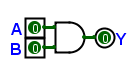
\includegraphics[width=\maxwidth{.95\linewidth}]{gfx/04_01}
	\caption{AND Gate}
	\label{fig:04_01}
\end{figure}

Notice that each input and output is named in order to make it easier to describe the circuit algebraically. In reality, \textsf{AND}  gates are not packaged or sold one at a time; rather, several would be placed on a single \gls{ic}, like the \emph{7408 Quad AND Gate}. The designer would design the circuit card to use whichever of the four gates are needed while leaving the unused gates unconnected. 

There are two common sets of symbols used to represent the various elements in logic diagrams, and whichever is used is of little consequence since the logic is the same. Shaped symbols, as used in Figure \ref{fig:04_01}, are more common in the United States; but the \gls{ieee} has its own symbols which are sometimes used, especially in Europe. Figure \ref{fig:04_02} illustrates the circuit in Figure \ref{fig:04_01} using \gls{ieee} symbols:

% Pull Quote - Marginal Note - Sidebar
\marginpar{In this book, only shaped symbols will be used.}

\begin{figure}[H]
	\centering
	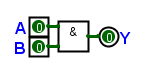
\includegraphics[width=\maxwidth{.95\linewidth}]{gfx/04_02}
	\caption{AND Gate Using IEEE Symbols}
	\label{fig:04_02}
\end{figure}

As an example of an \textsf{AND}  gate at work, consider an elevator: if the door is closed (logic $ 1 $) \textsf{AND} someone in the elevator car presses a floor button (logic $ 1 $), THEN the elevator will move (logic $ 1 $). If both sensors (door and button) are input to an \textsf{AND}  gate, then the elevator motor will only operate if the door is closed \textsf{AND}  someone presses a floor button. 

\subsection{OR}
\label{BF:subsec:or}

An \textsf{OR}  gate is a Boolean operation that will output a logical one, or \emph{True}, if any or all of the inputs are \emph{True}. As an example, consider this statement: ``If my dog needs a bath OR I am going swimming, then I will put on a bathing suit.'' In this statement, ``if my dog needs a bath'' is one input variable and ``I am going swimming'' is another input variable. If either of these is \emph{True}, then the output variable, ``I will put on a bathing suit,'' will also be \emph{True}. However, if both of the inputs are \emph{False}, then the output will also be \emph{False} (or, ``I will not put on a bathing suit''). If you think it odd that I would wear a bathing suit to bathe my dog then you have obviously never met my dog. 

When written in an equation, the Boolean \textsf{OR}  term is represented a number of different ways. One method is to use the logic \textsf{OR}  symbol, as found in Equation \ref{BF:eq:or_vee}.

\begin{align}
  \label{BF:eq:or_vee}
  A \vee B &= Y 
\end{align}

A more common method is to use the \emph{plus} sign that is used for addition in traditional algebra, as in Equation \ref{BF:eq:or_plus}.

\begin{align}
  \label{BF:eq:or_plus}
  A + B &= Y 
\end{align}

For simplicity, the mathematical \emph{plus} symbol is normally used to indicate \textsf{OR}  in printed material since it is easy to enter with a keyboard; however, if there is any chance for ambiguity, then the logic \textsf{OR}  symbol ($ \vee $) is used to differentiate between addition and logic \textsf{OR}.

Table \ref{BF:tab:truth_table_for_or} is the truth table for an \textsf{OR}  operation.

%******************************************************
% OR Truth Table
%******************************************************
\begin{table}[H]
  \sffamily
  \newcommand{\head}[1]{\textcolor{white}{\textbf{#1}}}    
  \begin{center}
    \rowcolors{2}{gray!10}{white} % Color every other line a light gray
    \begin{tabular}{ccc} 
      \rowcolor{black!75}
      \multicolumn{2}{c}{\head{Inputs}} & \head{Output} \\
      A & B & Y \\
      \hline
      0 & 0 & 0 \\
      0 & 1 & 1 \\
      1 & 0 & 1 \\
      1 & 1 & 1 
    \end{tabular}
  \end{center}
  \caption{Truth Table for OR}
  \label{BF:tab:truth_table_for_or}
\end{table}

Notice for the \textsf{OR} truth table that the output is \emph{True} ($ 1 $) whenever at least one input is \emph{True}. Therefore, it could be said that one \emph{True} input would activate an \textsf{OR} Gate. In the following diagram, the input variables $ A $ and $ B $ are wired to an \textsf{OR}  gate, and the output from that gate goes to $ Y $. 

\begin{figure}[H]
	\centering
	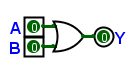
\includegraphics[width=\maxwidth{.95\linewidth}]{gfx/04_03}
	\caption{OR Gate}
	\label{fig:04_03}
\end{figure}

As an example of an \textsf{OR} gate at work, consider a traffic signal. Suppose an intersection is set up such that the light for the main road is normally green; however, if a car pulls up to the intersection from the crossroad, or if a pedestrian presses the ``cross'' button, then the main light is changed to red to stop traffic. This could be done with a simple \textsf{OR} gate. An automobile sensor on the crossroad would be one input and the pedestrian ``cross'' button would be the other input; the output of the \textsf{OR}  gate connecting these two inputs would change the light to red when either input is activated.

\subsection{NOT}
\label{BF:subsec:not}

\textsf{NOT} (or \emph{inverter}) is a Boolean operation that inverts the input. That is, if the input is \emph{True} then the output will be \emph{False} or if the input is \emph{False} then the output will be \emph{True}. When written in an equation, the Boolean \textsf{NOT}  operator is represented in many ways, though two are most popular. The older method is to overline (that is, a line above) a term, or group of terms, that are to be inverted, as in Equation \ref{BF:eq:not_bar}.\marginpar{Equation \ref{BF:eq:not_bar} is read \emph{A OR B NOT = Q} (notice that when spoken, the word \emph{not} follows the term that is inverted).}

\begin{align}
  \label{BF:eq:not_bar}
  A + \overline{B} &= Y 
\end{align}

Another method of indicating \textsf{NOT}  is to use the algebra \emph{prime} indicator, an apostrophe, as in Equation \ref{BF:eq:not_apostrophe}.

\begin{align}
  \label{BF:eq:not_apostrophe}
  A + B' &= Y 
\end{align}

The reason that \textsf{NOT} is most commonly indicated with an apostrophe is because that is easier to enter on a computer keyboard. There are many other ways authors use to represent \textsf{NOT}  in a formula, but none are considered standardized. For example, some authors use an exclamation point: $ A+!B=Q $, others use a broken line: $ A+ \neg B=Q $, others use a backslash: $ A+ \backslash B=Q $, and still others use a tilde: $ A+ \sim B =Q $. However, only the apostrophe and overline are consistently used to indicate \textsf{NOT}. Table \ref{BF:tab:truth_table_for_not} is the truth table for \textsf{NOT}:

%******************************************************
% NOT Truth Table
%******************************************************
\begin{table}[H]
  \sffamily
  \newcommand{\head}[1]{\textcolor{white}{\textbf{#1}}}    
  \begin{center}
    \rowcolors{2}{gray!10}{white} % Color every other line a light gray
    \begin{tabular}{ccc} 
      \rowcolor{black!75}
      \head{Input} & \head{Output} \\
      0 & 1 \\
      1 & 0 \\
    \end{tabular}
  \end{center}
  \caption{Truth Table for NOT}
  \label{BF:tab:truth_table_for_not}
\end{table}

In a logic diagram, \textsf{NOT}  is represented by a small triangle with a ``bubble'' on the output. In Figure \ref{fig:04_04}, the input variable $ A $ is inverted by a \textsf{NOT}  gate and then sent to output $ Y $. 

\begin{figure}[H]
	\centering
	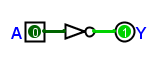
\includegraphics[width=\maxwidth{.95\linewidth}]{gfx/04_04}
	\caption{NOT Gate}
	\label{fig:04_04}
\end{figure}


%*********************************************************************
% NAND Gate
%*********************************************************************
\section{Secondary Logic Functions}
\label{BF:sec:secondary_logic_functions}
\subsection{NAND}
\label{BF:subsec:nand}

\textsf{NAND} is a Boolean operation that outputs the opposite of \textsf{AND}, that is, \textsf{NOT AND}; thus, it will output a logic \emph{False} only if all of the inputs are \emph{True}. The \textsf{NAND} operation is not often used in Boolean equations, but when necessary it is represented by a vertical line. Equation \ref{BF:eq:nand_symbol} shows a \textsf{NAND}  operation.

\begin{align}
  \label{BF:eq:nand_symbol}
  A | B &= Y 
\end{align}

Table \ref{BF:tab:truth_table_for_nand_gate} is the Truth Table for a \textsf{NAND}  gate.

%******************************************************
% NAND Truth Table
%******************************************************
\begin{table}[H]
  \sffamily
  \newcommand{\head}[1]{\textcolor{white}{\textbf{#1}}}    
  \begin{center}
    \rowcolors{2}{gray!10}{white} % Color every other line a light gray
    \begin{tabular}{ccc} 
      \rowcolor{black!75}
      \multicolumn{2}{c}{\head{Inputs}} & \head{Output} \\
      A & B & Y \\
      \hline
      0 & 0 & 1 \\
      0 & 1 & 1 \\
      1 & 0 & 1 \\
      1 & 1 & 0 
    \end{tabular}
  \end{center}
  \caption{Truth Table for \textsf{NAND}  Gate}
  \label{BF:tab:truth_table_for_nand_gate}
\end{table}

In Figure \ref{fig:04_05}, the input variables $ A $ and $ B $ are wired to a NAND gate, and the output from that gate goes to $ Y $.

\begin{figure}[H]
	\centering
	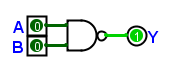
\includegraphics[width=\maxwidth{.95\linewidth}]{gfx/04_05}
	\caption{NAND Gate}
	\label{fig:04_05}
\end{figure}


\marginpar{Inverting bubbles are never found by themselves on a wire; they are always associated with either the inputs or output of a logic gate. To invert a signal on a wire, a \textsf{NOT} gate is used.}The logic diagram symbol for a \textsf{NAND}  gate looks like an \textsf{AND} gate, but with a small bubble on the output port. A bubble in a logic diagram always represents some sort of signal inversion, and it can appear at the inputs or outputs of nearly any logic gate. For example, the bubble on a \textsf{NAND}  gate could be interpreted as ``take whatever the output would be generated by an \textsf{AND} gate\textemdash then invert it.'' 

%*************************************************************
% NOR Gate
%*************************************************************
\subsection{NOR}
\label{BF:subsec:nor}

\textsf{NOR}  is a Boolean operation that is the opposite of OR, that is, \textsf{NOT OR}; thus, it will output a logic \emph{True} only if all of the inputs are \emph{False}. The \textsf{NOR} operation is not often used in Boolean equations, but when necessary it is represented by a downward-pointing arrow. Equation \ref{BF:eq:nor_symbol} shows a \textsf{NOR} operation.

\begin{align}
  \label{BF:eq:nor_symbol}
  A \downarrow B &= Y 
\end{align}

Table \ref{BF:tab:truth_table_for_nor} is the truth table for \textsf{NOR} . 

%******************************************************
% NOR Truth Table
%******************************************************
\begin{table}[H]
  \sffamily
  \newcommand{\head}[1]{\textcolor{white}{\textbf{#1}}}    
  \begin{center}
    \rowcolors{2}{gray!10}{white} % Color every other line a light gray
    \begin{tabular}{ccc} 
      \rowcolor{black!75}
      \multicolumn{2}{c}{\head{Inputs}} & \head{Output} \\
      A & B & Y \\
      \hline
      0 & 0 & 1 \\
      0 & 1 & 0 \\
      1 & 0 & 0 \\
      1 & 1 & 0 
    \end{tabular}
  \end{center}
  \caption{Truth Table for NOR}
  \label{BF:tab:truth_table_for_nor}
\end{table}

In Figure \ref{fig:04_06}, the input variables $ A $ and $ B $ are wired to a \textsf{NOR}  gate, and the output from that gate goes to $ Y $. 

\begin{figure}[H]
	\centering
	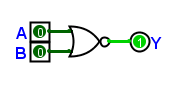
\includegraphics[width=\maxwidth{.95\linewidth}]{gfx/04_06}
	\caption{NOR Gate}
	\label{fig:04_06}
\end{figure}


\subsection{XOR}
\label{BF:subsec:xor}

\textsf{XOR} (\emph{Exclusive OR}) is a Boolean operation that outputs a logical one, or \emph{True}, only if the two inputs are different. This is useful for circuits that compare inputs; if they are different then the output is \emph{True}, otherwise it is \emph{False}. Because of this, an \textsf{XOR}  gate is sometimes referred to as a \emph{Difference Gate}. The \textsf{XOR} operation is not often used in Boolean equations, but when necessary it is represented by a plus sign (like the OR function) inside a circle. Equation \ref{BF:eq:xor_symbol} shows an \textsf{XOR}  operation.

% XOR in equation
\begin{align}
  \label{BF:eq:xor_symbol}
  A \oplus B &= Y
\end{align}

Table \ref{BF:tab:truth_table_for_xor} is the truth table for an \textsf{XOR}  gate.

%******************************************************
% XOR Truth Table
%******************************************************
\begin{table}[H]
  \sffamily
  \newcommand{\head}[1]{\textcolor{white}{\textbf{#1}}}    
  \begin{center}
    \rowcolors{2}{gray!10}{white} % Color every other line a light gray
    \begin{tabular}{ccc} 
      \rowcolor{black!75}
      \multicolumn{2}{c}{\head{Inputs}} & \head{Output} \\
      A & B & Y \\
      \hline
      0 & 0 & 0 \\
      0 & 1 & 1 \\
      1 & 0 & 1 \\
      1 & 1 & 0 
    \end{tabular}
  \end{center}
  \caption{Truth Table for XOR}
  \label{BF:tab:truth_table_for_xor}
\end{table}

In Figure \ref{fig:04_07}, the input variables $ A $ and $ B $ are wired to an \textsf{XOR}  gate, and the output from that gate goes to $ Y $. 

\begin{figure}[H]
	\centering
	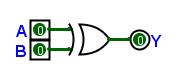
\includegraphics[width=\maxwidth{.95\linewidth}]{gfx/04_07}
	\caption{XOR Gate}
	\label{fig:04_07}
\end{figure}


There is some debate about the proper behavior of an \textsf{XOR}  gate that has more than two inputs. Some experts believe that an \textsf{XOR} gate should output a \emph{True} if one, and only one, input is \emph{True} regardless of the number of inputs. This would seem to be in keeping with the rules of digital logic developed by George Boole and other early logisticians and is the strict definition of \textsf{XOR} promulgated by the \gls{ieee}. This is also the behavior of the \textsf{XOR} gate found in \textit{Logisim-evolution}, the digital logic simulator used in the lab manual accompanying this text. Others believe, though, that an \textsf{XOR} gate should output a \emph{True} if an odd number of inputs is \emph{True}. in \Le this type of behavior is found in a device called a ``parity gate'' and is covered in more detail elsewhere in this book.

%**********************************************************
% XNOR Gate
%**********************************************************
\subsection{XNOR}
\label{BF:subsec:xnor}

\textsf{XNOR} is a Boolean operation that will output a logical one, or \emph{True}, only if the two inputs are the same; thus, an \textsf{XNOR} gate is often referred to as an \emph{Equivalence Gate}. The \textsf{XNOR} operation is not often used in Boolean equations, but when necessary it is represented by a dot inside a circle. Equation \ref{BF:eq:xnor_symbol} shows an \textsf{XNOR}  operation. 

% XNOR in equation
\begin{align}
  \label{BF:eq:xnor_symbol}
  A \odot B &= Y
\end{align}

Table \ref{BF:tab:truth_table_for_xnor} is the truth table for \textsf{XNOR} . 

%******************************************************
% XNOR Truth Table
%******************************************************
\begin{table}[H]
  \sffamily
  \newcommand{\head}[1]{\textcolor{white}{\textbf{#1}}}    
  \begin{center}
    \rowcolors{2}{gray!10}{white} % Color every other line a light gray
    \begin{tabular}{ccc} 
      \rowcolor{black!75}
      \multicolumn{2}{c}{\head{Inputs}} & \head{Output} \\
      A & B & Y \\
      \hline
      0 & 0 & 1 \\
      0 & 1 & 0 \\
      1 & 0 & 0 \\
      1 & 1 & 1 
    \end{tabular}
  \end{center}
  \caption{Truth Table for XNOR}
  \label{BF:tab:truth_table_for_xnor}
\end{table}

In Figure \ref{fig:04_08}, the input variables $ A $ and $ B $ are wired to an \textsf{XNOR}  gate, and the output from that gate goes to $ Y $. 

\begin{figure}[H]
	\centering
	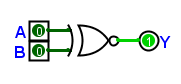
\includegraphics[width=\maxwidth{.95\linewidth}]{gfx/04_08}
	\caption{XNOR Gate}
	\label{fig:04_08}
\end{figure}


\subsection{Buffer}
\label{BF:subsec:buffer}

A buffer (sometimes called \emph{Transfer}) is a Boolean operation that transfers the input to the output without change. If the input is \emph{True}, then the output will be \emph{True} and if the input is \emph{False}, then the output will be \emph{False}. It may seem to be an odd function since this operation does not change anything, but it has an important use in a circuit. As logic circuits become more complex, the signal from input to output may become weak and no longer able to drive (or activate) additional gates. A buffer is used to boost (and stabilize) a logic level so it is more dependable. Another important function for a buffer is to clean up an input signal. As an example, when an electronic circuit interacts with the physical world (such as a user pushing a button), there is often a very brief period when the signal from that physical device waivers between high and low unpredictably. A buffer can smooth out that signal so it is a constant high or low without voltage spikes in between. 

Table \ref{BF:tab:truth_table_for_a_buffer} is the truth table for buffer.

%******************************************************
% Buffer Truth Table
%******************************************************
\begin{table}[H]
  \sffamily
  \newcommand{\head}[1]{\textcolor{white}{\textbf{#1}}}    
  \begin{center}
    \rowcolors{2}{gray!10}{white} % Color every other line a light gray
    \begin{tabular}{ccc} 
      \rowcolor{black!75}
      \head{Input} & \head{Output} \\
      0 & 0 \\
      1 & 1 
    \end{tabular}
  \end{center}
  \caption{Truth Table for a Buffer}
  \label{BF:tab:truth_table_for_a_buffer}
\end{table}

Buffers are rarely used in schematic diagrams since they do not actually change a signal; however, Figure \ref{fig:04_09}, illustrates a buffer. 

\begin{figure}[H]
	\centering
	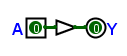
\includegraphics[width=\maxwidth{.95\linewidth}]{gfx/04_09}
	\caption{Buffer}
	\label{fig:04_09}
\end{figure}

\section{Univariate Boolean Algebra Properties}
\label{BF:sec:univariate_boolean_algebra_properties}
\subsection{Introduction}
\label{BF:subsec:introduction_to_univariate}

Boolean Algebra, like real number algebra, includes a number of properties. This unit introduces the univariate Boolean properties, or those properties that involve only one input variable. These properties permit Boolean expressions to be simplified, and circuit designers are interested in simplifying circuits to reduce construction expense, power consumption, heat loss (wasted energy), and troubleshooting time.  

\subsection{Identity}
\label{BF:subsec:identity}

In mathematics, an identity is an equality where the left and right members are the same regardless of the values of the variables present. As an example, Equation \ref{BF:eq:identity_example} is an identity since the two members are identical regardless of the value of $ \alpha $:

\begin{align}
  \label{BF:eq:identity_example}
  \frac{\alpha}{2} &= 0.5\alpha
\end{align}

An \emph{Identity Element} is a special member of a set such that when that element is used in a binary operation the other element in that operation is not changed. This is sometimes called the \emph{Neutral Element} since it has no effect on binary operations. As an example, in Equation \ref{BF:eq:identity_element_of_addition} the two members of the equation are always identical. Therefore, zero is the identity element for addition since anything added to zero remains unchanged.

\begin{align}
  \label{BF:eq:identity_element_of_addition}
  a + 0 &= a 
\end{align}

In a logic circuit, combining any logic input with a logic zero through an \textsf{OR}  gate yields the original input. Logic zero, then, is considered the \textsf{OR} identity element because it causes the input of the gate to be copied to the output unchanged. Because \textsf{OR}  is represented by a plus sign when written in a Boolean equation, and the identity element for \textsf{OR}  is zero, Equation \ref{BF:eq:or_identity} is \emph{True}.

\begin{align}
  \label{BF:eq:or_identity}
  A + 0 &= A 
\end{align}

The bottom input to the \textsf{OR} gate in \ref{fig:04_10} is a constant logic zero, or \emph{False}. The output for this circuit, $ Y $, will be the same as input $ A $; therefore, the identity element for \textsf{OR}  is zero.  

\begin{figure}[H]
	\centering
	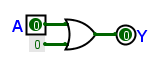
\includegraphics[width=\maxwidth{.95\linewidth}]{gfx/04_10}
	\caption{OR Identity Element}
	\label{fig:04_10}
\end{figure}

In the same way, combining any logic input with a logic one through an \textsf{AND}  gate yields the original input. Logic one, then, is considered the \textsf{AND}  identity element because it causes the input of the gate to be copied to the output unchanged. Because \textsf{AND}  is represented by a multiplication sign when written in a Boolean equation, and the identity element for \textsf{AND} is one, Equation \ref{BF:eq:and_identity} is \emph{True}.

\begin{align}
  \label{BF:eq:and_identity}
  A * 1 &= A 
\end{align}

The bottom input to the \textsf{AND} gate in \ref{fig:04_11} is a constant logic one, or \emph{True}. The output for this circuit, $ Y $, will be the same as input $ A $; therefore, the identity element for \textsf{AND}  is one.  

\begin{figure}[H]
	\centering
	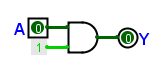
\includegraphics[width=\maxwidth{.95\linewidth}]{gfx/04_11}
	\caption{AND Identity Element}
	\label{fig:04_11}
\end{figure}

\subsection{Idempotence}
\label{BF:subsec:idempotence}

If the two inputs of either an \textsf{OR} or \textsf{AND} gate are tied together, then the same signal will be applied to both inputs. This results in the output of either of those gates being the same as the input; and this is called the idempotence property. An electronic gate wired in this manner performs the same function as a buffer. 

% Pull Quote - Marginal Note - Sidebar
\marginpar{Remember that in Boolean expressions a plus sign represents an \textsf{OR}  gate, not mathematical addition.}

\begin{align}
  \label{BF:eq:idempotence_for_or}
  A + A &= A 
\end{align}

\begin{figure}[H]
	\centering
	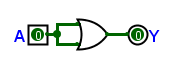
\includegraphics[width=\maxwidth{.95\linewidth}]{gfx/04_12}
	\caption{Idempotence Property for OR Gate}
	\label{fig:04_12}
\end{figure}

Figure \ref{fig:04_12} illustrates the idempotence property for an \textsf{AND} gate.

% Pull Quote - Marginal Note - Sidebar
\marginpar{Remember that in a Boolean expression a multiplication sign represents an AND gate, not mathematical multiplying.}

\begin{align}
  \label{BF:eq:idempotence_for_and}
  A * A &= A 
\end{align}

\begin{figure}[H]
	\centering
	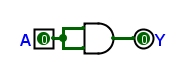
\includegraphics[width=\maxwidth{.95\linewidth}]{gfx/04_13}
	\caption{Idempotence Property for AND Gate}
	\label{fig:04_13}
\end{figure}

\subsection{Annihilator}
\label{BF:subsec:annihilator}

Combining any data and a logic one through an \textsf{OR} gate yields a constant output of one. This property is called the annihilator since the \textsf{OR} gate outputs a constant one; in other words, whatever other data were input are lost. Because \textsf{OR} is represented by a plus sign when written in a Boolean equation, and the annihilator for \textsf{OR} is one, the following is true:

\begin{align}
  \label{BF:eq:annihilator_or}
  A + 1 &= 1 
\end{align}

\begin{figure}[H]
	\centering
	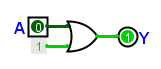
\includegraphics[width=\maxwidth{.95\linewidth}]{gfx/04_14}
	\caption{Annihilator For OR Gate}
	\label{fig:04_14}
\end{figure}

The bottom input for the \textsf{OR}  gate in Figure \ref{fig:04_14} is a constant logic one, or \emph{True}. The output for this circuit will be \emph{True} (or $ 1 $) no matter whether input $ A $ is \emph{True} or \emph{False} ($ 1 $ or $ 0 $).

Combining any data and a logic zero with an \textsf{AND} gate yields a constant output of zero. This property is called the annihilator since the \textsf{AND}  gate outputs a constant zero; in other words, whatever logic data were input are lost. Because \textsf{AND}  is represented by a multiplication sign when written in a Boolean equation, and the annihilator for \textsf{AND} is zero, the following is true:

\begin{align}
  \label{BF:eq:annihilator_and}
  A * 0 &= 0 
\end{align}

\begin{figure}[H]
	\centering
	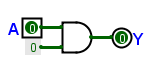
\includegraphics[width=\maxwidth{.95\linewidth}]{gfx/04_15}
	\caption{Annihilator For AND Gate}
	\label{fig:04_15}
\end{figure}

The bottom input for the \textsf{AND} gate in Figure \ref{fig:04_15} is a constant logic zero, or \emph{False}. The output for this circuit will be \emph{False} (or $ 0 $) no matter whether input $ A $ is \emph{True} or \emph{False} ($ 1 $ or $ 0 $).

\subsection{Complement}
\label{BF:subsec:complement}

In Boolean logic there are only two possible values for variables: $ 0 $ and $ 1 $. Since either a variable or its complement must be one, and since combining any data with one through an \textsf{OR} gate yields one (see the Annihilator in Equation \ref{BF:eq:annihilator_or}), then the following is true:

\begin{align}
  \label{BF:eq:complement_or}
  A + A' &= 1 
\end{align}

\begin{figure}[H]
	\centering
	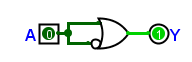
\includegraphics[width=\maxwidth{.95\linewidth}]{gfx/04_16}
	\caption{OR Complement}
	\label{fig:04_16}
\end{figure}

In Figure \ref{fig:04_16}, the output ($ Y $) will always equal one, regardless of the value of input $ A $. This leads to the general property that when a variable and its complement are combined through an \textsf{OR} gate the output will always be one. 

In the same way, since either a variable or its complement must be zero, and since combining any data with zero through an \textsf{AND} gate yields zero (see the Annihilator in Equation \ref{BF:eq:annihilator_and}), then the following is true: 

\begin{align}
  \label{BF:eq:complement_and}
  A * A' &= 0
\end{align}

\begin{figure}[H]
	\centering
	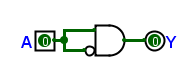
\includegraphics[width=\maxwidth{.95\linewidth}]{gfx/04_17}
	\caption{AND Complement}
	\label{fig:04_17}
\end{figure}

\subsection{Involution}
\label{BF:subsec:involution}

\marginpar{The Involution Property is sometimes called the ``Double Complement'' Property.}

Another law having to do with complementation is that of Involution. Complementing a Boolean variable two times (or any even number of times) results in the original Boolean value. 

\begin{align}
  \label{BF:eq:involuton}
  (A')' &= A
\end{align}

\begin{figure}[H]
	\centering
	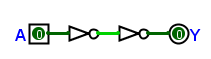
\includegraphics[width=\maxwidth{.95\linewidth}]{gfx/04_18}
	\caption{Involution Property}
	\label{fig:04_18}
\end{figure}

In the circuit illustrated in Figure \ref{fig:04_18}, the output ($ Y $) will always be the same as the input ($ A $). 

% Begin Sidebar Box
\begin{tcolorbox}[colback=blue!5!white,colframe=blue!75!black]
  % Upper half of box: my "title" area
  \textcolor{blue}{\textbf{Propagation Delay}}
  % Lower half of the box: the content
  \tcblower
  It takes the two \textsf{NOT} gates a short period of time to pass a signal from input to output, which is known as ``propagation delay.'' A designer occasionally needs to build an intentional signal delay into a circuit for some reason and two (or any even number of) consecutive \textsf{NOT} gates would be one option.
\end{tcolorbox}
% End Sidebar Box

\section{Multivariate Boolean Algebra Properties}
\label{BF:sec:multivariate_boolean_algebra_properties}
\subsection{Introduction}
\label{BF:subsec:introduction_to_multivariate}

Boolean Algebra, like real number algebra, includes a number of properties. This unit introduces the multivariate Boolean properties, or those properties that involve more than one input variable. These properties permit Boolean expressions to be simplified, and circuit designers are interested in simplifying circuits to reduce construction expense, power consumption, heat loss (wasted energy), and troubleshooting time.  

\subsection{Commutative}
\label{BF:subsec:commutative_property}

\marginpar{The examples here show only two variables, but this property is true for any number of variables.}

In essence, the commutative property indicates that the order of the input variables can be reversed in either \textsf{OR} or \textsf{AND} gates without changing the truth of the expression. Equation \ref{BF:eq:commutative} expresses this property algebraically.

\begin{align}
  \label{BF:eq:commutative}
  A + B &= B + A \\
  \nonumber
  A * B &= B * A
\end{align}

\begin{figure}[H]
	\centering
	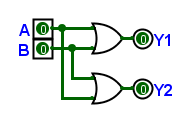
\includegraphics[width=\maxwidth{.95\linewidth}]{gfx/04_19}
	\caption{Commutative Property for OR}
	\label{fig:04_19}
\end{figure}

\marginpar{\textsf{XOR} and \textsf{XNOR} are also commutative; but for only two variables, not three or more.}

\begin{figure}[H]
	\centering
	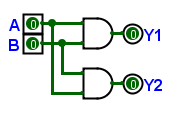
\includegraphics[width=\maxwidth{.95\linewidth}]{gfx/04_20}
	\caption{Commutative Property for AND}
	\label{fig:04_20}
\end{figure}

In Figures \ref{fig:04_19} and \ref{fig:04_20} the inputs are reversed for the two gates, but the outputs are the same. For example, $ A $ is entering the top input for the upper \textsf{OR} gate, but the bottom input for the lower gate; however, $ Y1 $ is always equal to $ Y2 $.

\subsection{Associative}
\label{BF:subsec:associative_property}

\marginpar{The examples here show only three variables, but this property is true for any number of variables.}

This property indicates that groups of variables in an \textsf{OR} or \textsf{AND} gate can be associated in various ways without altering the truth of the equations. Equation \ref{BF:eq:associative} expresses this property algebraically: 

\begin{align}
  \label{BF:eq:associative}
  ( A + B ) + C &= A + ( B + C ) \\
  \nonumber
  ( A * B ) * C &= A * ( B * C )
\end{align}

\marginpar{\textsf{XOR} and \textsf{XNOR} are also associative; but for only two variables, not three or more.}

In the circuits in Figure \ref{fig:04_21} and \ref{fig:04_22} , notice that $ A $ and $ B $ are associated together in the first gate, and then $ C $ is associated with the output of that gate. Then, in the lower half of the circuit, $ B $ and $ C $ are associated together in the first gate, and then $ A $ is associated with the output of that gate. Since $ Y1 $ is always equal to $ Y2 $ for any combination of inputs, it does not matter which of the two variables are associated together in a group of gates.  

\begin{figure}[H]
	\centering
	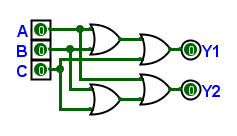
\includegraphics[width=\maxwidth{.95\linewidth}]{gfx/04_21}
	\caption{Associative Property for OR}
	\label{fig:04_21}
\end{figure}

\begin{figure}[H]
	\centering
	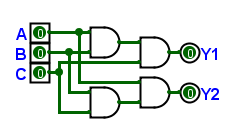
\includegraphics[width=\maxwidth{.95\linewidth}]{gfx/04_22}
	\caption{Associative Property for AND}
	\label{fig:04_22}
\end{figure}

\subsection{Distributive}
\label{BF:subsec:distributive_property}

The distributive property of real number algebra permits certain variables to be ``distributed'' to other variables. This operation is frequently used to create groups of variables that can be simplified; thus, simplifying the entire expression. Boolean algebra also includes a distributive property, and that can be used to combine \textsf{OR}  or \textsf{AND}  gates in various ways that make it easier to simplify the circuit. Equation \ref{BF:eq:distributive} expresses this property algebraically:

\begin{align}
  \label{BF:eq:distributive}
  A( B + C ) &= AB + AC \\
  \nonumber
  A + (BC) &= (A + B) (A + C)
\end{align}

In the circuits illustrated in Figures \ref{fig:04_23} and \ref{fig:04_24}, notice that input $ A $ in the top half of the circuit is distributed to inputs $ B $ and $ C $ in the bottom half. However, output $ Y1 $ is always equal to output $ Y2 $ regardless of how the inputs are set. These two circuits illustrate Distributive of \textsf{AND} over \textsf{OR}  and Distributive of \textsf{OR} over \textsf{AND} .
 
\begin{figure}[H]
	\centering
	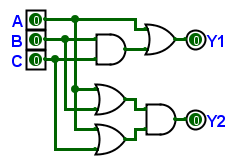
\includegraphics[width=\maxwidth{.95\linewidth}]{gfx/04_23}
	\caption{Distributive Property for AND over OR}
	\label{fig:04_23}
\end{figure}

\begin{figure}[H]
	\centering
	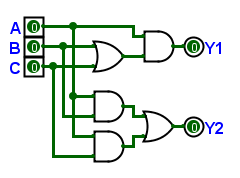
\includegraphics[width=\maxwidth{.95\linewidth}]{gfx/04_24}
	\caption{Distributive Property for OR over AND}
	\label{fig:04_24}
\end{figure}

\subsection{Absorption}
\label{BF:subsec:absorption_property}

The absorption property is used to remove logic gates from a circuit if those gates have no effect on the output. In essence, a gate is ``absorbed'' if it is not needed. There are two different absorption properties:

\begin{align}
  \label{BF:eq:absorption}
  A + (AB) &= A \\
  \nonumber
  A(A + B) &= A
\end{align}

The best way to think about why these properties are true is to imagine a circuit that contains them. The first circuit below illustrates the top equation. 

\begin{figure}[H]
	\centering
	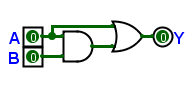
\includegraphics[width=\maxwidth{.95\linewidth}]{gfx/04_25}
	\caption{Absorption Property (Version 1)}
	\label{fig:04_25}
\end{figure}

Table \ref{BF:tab:truth_table_for_absorption_property_version_1} is the truth table for the circuit in Figure \ref{fig:04_25}.

%******************************************************
% Absorption (Version 1) Truth Table
%******************************************************
\begin{table}[H]
  \sffamily
  \newcommand{\head}[1]{\textcolor{white}{\textbf{#1}}}    
  \begin{center}
    \rowcolors{2}{gray!10}{white} % Color every other line a light gray
    \begin{tabular}{ccc} 
      \rowcolor{black!75}
      \multicolumn{2}{c}{\head{Inputs}} & \head{Output} \\
      A & B & Y \\
      \hline
      0 & 0 & 0 \\
      0 & 1 & 0 \\
      1 & 0 & 1 \\
      1 & 1 & 1 
    \end{tabular}
  \end{center}
  \caption{Truth Table for Absorption Property}
  \label{BF:tab:truth_table_for_absorption_property_version_1}
\end{table}

Notice that the output, $ Y $, is always the same as input $ A $. This means that input $ B $ has no bearing on the output of the circuit; therefore, the circuit could be replaced by a piece of wire from input $ A $ to output $ Y $. Another way to state that is to say that input $ B $ is absorbed by the circuit.

The circuit illustrated in Figure \ref{fig:04_26} is the second version of the Absorption Property. Like the first Absorption Property circuit, a truth table would demonstrate that input $ B $ is absorbed by the circuit. 

\begin{figure}[H]
	\centering
	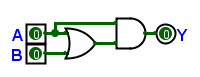
\includegraphics[width=\maxwidth{.95\linewidth}]{gfx/04_26}
	\caption{Absorption Property (Version 2)}
	\label{fig:04_26}
\end{figure}

\subsection{Adjacency}
\label{BF:subsec:adjacency_property}

The adjacency property simplifies a circuit by removing unnecessary gates.

\begin{align}
  \label{BF:eq:adjacency}
  AB + AB' &= A
\end{align}

This property can be proven by simple algebraic manipulation:

\begin{align}
  \label{BF:eq:adjacency_solved}
  AB + AB' && \text{Original Expression} \\
  \nonumber
  A ( B + B') && \text{Distributive Property} \\
  \nonumber
  A1 && \text{Complement Property} \\
  \nonumber
  A && \text{Identity Element}
\end{align}

The circuit in Figure \ref{fig:04_27} illustrates the adjacency property. If this circuit were constructed it would be seen that the output, $ Y $, is always the same as input $ A $; therefore, this entire circuit could be replaced by a single wire from input $ A $ to output $ Y $.

\begin{figure}[H]
	\centering
	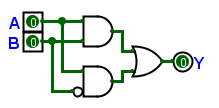
\includegraphics[width=\maxwidth{.95\linewidth}]{gfx/04_27}
	\caption{Adjacency Property}
	\label{fig:04_27}
\end{figure}

\section{DeMorgan's Theorem}
\label{BF:sec:demorgans_theorem}
\subsection{Introduction}
\label{BF:subsec:introduction_demorgans}

A mathematician named Augustus DeMorgan developed a pair of important theorems regarding the complementation of groups in Boolean algebra. DeMorgan found that an \textsf{OR} gate with all inputs inverted (a Negative-\textsf{OR} gate) behaves the same as a \textsf{NAND}  gate with non-inverted inputs; and an \textsf{AND} gate with all inputs inverted (a Negative-\textsf{AND} gate) behaves the same as a \textsf{NOR} gate with non-inverted inputs. DeMorgan's theorem states that inverting the output of any gate is the same as using the opposite type of gate with inverted inputs. Figure \ref{fig:04_28} illustrates this in circuit terms: the \textsf{NAND} gate with normal inputs and the \textsf{OR} gate with inverted inputs are functionally equivalent; that is, $ Y1 $ will always equal $ Y2 $, regardless of the values of input $ A $ or $ B $.  

\begin{figure}[H]
	\centering
	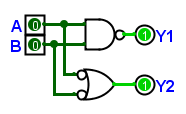
\includegraphics[width=\maxwidth{.95\linewidth}]{gfx/04_28}
	\caption{DeMorgan's Theorem Defined}
	\label{fig:04_28}
\end{figure}

The NOT function is commonly represented in an equation as an apostrophe because it is easy to enter with a keyboard, like: $ (AB)' $ for \emph{A AND B NOT}. However, it is easiest to work with DeMorgan's theorem if \textsf{NOT} is represented by an overline rather than an apostrophe, so it would be written as $ \overline{AB} $ rather than $ (AB)' $. Remember that an overline is a grouping symbol (like parenthesis) and it means that everything under that bar would first be combined (using an \textsf{AND} or \textsf{OR} gate) and then the output of the combination would be complemented.

\subsection{Applying DeMorgan's Theorem}
\label{BF:subsec:applying_demorgans_theorem}

Applying DeMorgan's theorem to a Boolean expression may be thought of in terms of \emph{breaking the bar}. When applying DeMorgan's theorem to a Boolean expression:

\begin{enumerate}
\item A complement bar is broken over a group of variables.
\item The operation (\textsf{AND}  or \textsf{OR} ) directly underneath the broken bar changes.
\item Pieces of the broken bar remain over the individual variables. 
\end{enumerate}

To illustrate:

\begin{align}
  \label{BF:eq:demorgan_nand}
  \overline{A*B} \leftrightarrow \overline{A}+\overline{B}
\end{align}

\begin{align}
  \label{BF:eq:demorgan_nor}
  \overline{A+B} \leftrightarrow \overline{A}*\overline{B}
\end{align}

Equation \ref{BF:eq:demorgan_nand} shows how a two-input \textsf{NAND} gate is ``broken'' to form an \textsf{OR} gate with two inverted inputs and equation \ref{BF:eq:demorgan_nor} shows how a two-input \textsf{NOR} gate is ``broken'' to form an \textsf{AND} gate with two complemented inputs.

\subsection{Simple Example}
\label{BF:subsec:simple_example_demorgan}

When multiple ``layers'' of bars exist in an expression, only one bar is broken at a time, and the longest, or uppermost, bar is broken first. As an example, consider the circuit in Figure \ref{fig:04_29}: 

\begin{figure}[H]
	\centering
	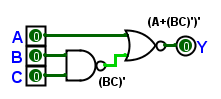
\includegraphics[width=\maxwidth{.95\linewidth}]{gfx/04_29}
	\caption{DeMorgan's Theorem Example 1}
	\label{fig:04_29}
\end{figure}

By writing the output at each gate (as illustrated in Figure \ref{fig:04_29}), it is easy to determine the Boolean expression for the circuit. Note: all circuit diagrams in this book are generated with \Le and the text tool in that software does not permit drawing overbars. Therefore, the circuit diagram will use the apostrophe method of indicating NOT but overbars will be used in the text.

\begin{align}
  \label{BF:eq:demorgan_simple_example}
  \overline{A+\overline{BC}}
\end{align}

To simplify the circuit, break the bar covering the entire expression (the ``longest bar''), and then simplify the resulting expression.

\begin{align}
  \label{BF:eq:demorgan_simple_solved}
  \overline{A+\overline{BC}} && \text{Original Expression} \\
  \nonumber
  \overline{A}\,\overline{\overline{BC}} && \text{''Break'' the longer bar} \\
  \nonumber
  \overline{A}BC && \text{Involution Property}
\end{align}

As a result, the original circuit is reduced to a three-input \textsf{AND} gate with one inverted input.

\subsection{Incorrect Application of DeMorgan's Theorem}
\label{BF:subsec:incorrect_application_of_demorgans_theorem}

More than one bar is never broken in a single step, as illustrated in Equation \ref{BF:eq:demorgan_incorrect_solution}: 

\begin{align}
  \label{BF:eq:demorgan_incorrect_solution}
  \overline{A+\overline{BC}} && \text{Original Expression} \\
  \nonumber
  \overline{A\overline{B}}+\overline{\overline{C}} && \text{Improperly Breaking Two Bars} \\
  \nonumber
  \overline{A}B+C && \text{Incorrect Solution}
\end{align}

Thus, as tempting as it may be to take a shortcut and break more than one bar at a time, it often leads to an incorrect result. Also, while it is possible to properly reduce an expression by breaking the short bar first; more steps are usually required and that process is not recommended.  

\subsection{About Grouping}
\label{BF:subsec:demorgans_about_grouping}

An important, but easily neglected, aspect of DeMorgan's theorem concerns grouping. Since a bar functions as a grouping symbol, the variables formerly grouped by a broken bar must remain grouped or else proper precedence (order of operation) will be lost. Therefore, after simplifying a large grouping of variables, it is a good practice to place them in parentheses in order to keep the order of operation the same.  

Consider the circuit in Figure \ref{fig:04_30}.

\begin{figure}[H]
	\centering
	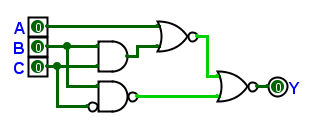
\includegraphics[width=\maxwidth{.95\linewidth}]{gfx/04_30}
	\caption{DeMorgan's Theorem Example 2}
	\label{fig:04_30}
\end{figure}

As always, the first step in simplifying this circuit is to generate the Boolean expression for the circuit, which is done by writing the sub-expression at the output of each gate. That results in Expression \ref{BF:eq:demorgan_grouping_solution}, which is then simplified. 

\begin{align}
  \label{BF:eq:demorgan_grouping_solution}
  \overline{ \overline{A+BC} + \overline{A \overline{B}}} && \text{Original Expression} \\
  \nonumber
  ( \overline{\overline{A+BC}} ) ( \overline{\overline{A\overline{B}}} ) && \text{Breaking the Longest Bar} \\
  \nonumber
  (A+BC)(A\overline{B}) && \text{Involution} \\
  \nonumber
  (AA\overline{B}) (BCA\overline{B}) && \text{Distribute $ A\overline{B} $ to $ (A+BC) $} \\
  \nonumber
  (A\overline{B})+(BCA\overline{B}) && \text{Idempotence: $ AA=A $} \\
  \nonumber
  (A\overline{B})+(0CA)) && \text{Complement: $ B\overline{B}=0 $} \\
  \nonumber
  (A\overline{B})+0 && \text{Annihilator: $ 0CA=0 $} \\
  \nonumber
  A\overline{B} && \text{Identity: $ A+0=A $}
\end{align}

The equivalent gate circuit for this much-simplified expression is as follows:

\begin{figure}[H]
	\centering
	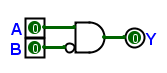
\includegraphics[width=\maxwidth{.95\linewidth}]{gfx/04_31}
	\caption{DeMorgan's Theorem Example 2 Simplified}
	\label{fig:04_31}
\end{figure}

\subsection{Summary}
\label{BF:subsec:demorgans_summary}

Here are the important points to remember about DeMorgan's Theorem: 

\begin{itemize}
  \item It describes the equivalence between gates with inverted inputs and gates with inverted outputs. 
  \item When "breaking" a complementation (or \textsf{NOT}) bar in a Boolean expression, the operation directly underneath the break (\textsf{AND} or \textsf{OR}) reverses and the broken bar pieces remain over the respective terms. 
  \item It is normally easiest to approach a problem by breaking the longest (uppermost) bar before breaking any bars under it. 
  \item Two complementation bars are never broken in one step. 
  \item Complementation bars function as grouping symbols. Therefore, when a bar is broken, the terms underneath it must remain grouped. Parentheses may be placed around these grouped terms as a help to avoid changing precedence.
\end{itemize}

\subsection{Example Problems}
\label{BF:subsec:demorgans_example_problems}

The following examples use DeMorgan's Theorem to simplify a Boolean expression.

%******************************************************
% DeMorgan's Problems
%******************************************************
\begin{table}[H]
  \newcommand{\head}[1]{\textcolor{white}{\textbf{#1}}}    
  \begin{center}
    \rowcolors{2}{gray!10}{white} % Color every other line a light gray
    \begin{tabular}{c|cc} 
      \rowcolor{black!75}
      & \head{Original Expression} & \head{Simplified} \\
      1 & $ (\overline{A+B})(\overline{ABC})(\overline{\overline{A}C}) $ 
        & $ \overline{A}\,\overline{B}\,\overline{C} $ \\
      2 & $ \overline{(AB+\overline{B}C)+(B\overline{C}+\overline{A}B)} $ 
        & $ \overline{B}\,\overline{C} $ \\
      3 & $ (AB+\overline{B}C)(AC+\overline{A}\,\overline{C}) $ 
        & $ \overline{A}+\overline{C} $ 
    \end{tabular}
  \end{center}
  \label{BF:tab:demorgans_example_problems}
  \sffamily
\end{table}

\section{Boolean Functions}
\label{BF:sec:boolean_functions}

Consider Figure \ref{fig:04_32}, which is a generic circuit with two inputs and one output.

\begin{figure}[H]
	\centering
	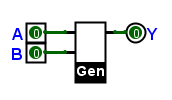
\includegraphics[width=\maxwidth{.95\linewidth}]{gfx/04_32}
	\caption{Generic Function}
	\label{fig:04_32}
\end{figure}

Without knowing anything about what is in the unlabeled box at the center of the circuit, there are a number of possible truth tables which could describe the circuit's output. Two possibilities are shown in Truth Table \ref{BF:tab:truth_table_for_generic_circuit_one} and Truth Table \ref{BF:tab:truth_table_for_generic_circuit_two}.

%******************************************************
% Generic Truth Table 1
%******************************************************
\begin{table}[H]
  \sffamily
  \newcommand{\head}[1]{\textcolor{white}{\textbf{#1}}}    
  \begin{center}
    \rowcolors{2}{gray!10}{white} % Color every other line a light gray
    \begin{tabular}{ccc} 
      \rowcolor{black!75}
      \multicolumn{2}{c}{\head{Inputs}} & \head{Output} \\
      A & B & Y \\
      \hline
      0 & 0 & 0 \\
      0 & 1 & 1 \\
      1 & 0 & 0 \\
      1 & 1 & 1 
    \end{tabular}
  \end{center}
  \caption{Truth Table for Generic Circuit One}
  \label{BF:tab:truth_table_for_generic_circuit_one}
\end{table}

%******************************************************
% Generic Truth Table 2
%******************************************************
\begin{table}[H]
  \sffamily
  \newcommand{\head}[1]{\textcolor{white}{\textbf{#1}}}    
  \begin{center}
    \rowcolors{2}{gray!10}{white} % Color every other line a light gray
    \begin{tabular}{ccc} 
      \rowcolor{black!75}
      \multicolumn{2}{c}{\head{Inputs}} & \head{Output} \\
      A & B & Y \\
      \hline
      0 & 0 & 0 \\
      0 & 1 & 1 \\
      1 & 0 & 1 \\
      1 & 1 & 0 
    \end{tabular}
  \end{center}
  \caption{Truth Table for Generic Circuit Two}
  \label{BF:tab:truth_table_for_generic_circuit_two}
\end{table}

In fact, there are $ 16 $ possible truth tables for this circuit. Each of those truth tables reflect a single potential function of the circuit by setting various combinations of input/output. Therefore, any two-input, one-output circuit has $ 16 $ possible functions. It is easiest to visualize all $ 16 $ combinations of inputs/outputs by using an odd-looking truth table. Consider only one of those $ 16 $ functions, the one for the generic circuit described by Truth Table \ref{BF:tab:truth_table_for_generic_circuit_two}. That function is also found in the Boolean Functions Table \ref{BF:tab:boolean_functions} and one row from that table is reproduced in Table \ref{BF:tab:boolean_function_six}.

\begin{table}[H]
  \sffamily
  \newcommand{\head}[1]{\textcolor{white}{\textbf{#1}}}    
  \begin{center}
    %\rowcolors{2}{gray!10}{white} % Color every other line a light gray
    \begin{tabular}{llllll}
      \textbf{A} & 0 & \cellcolor{gray!10}0 & 1 & 1 &  \\ 
      \textbf{B} & 0 & \cellcolor{gray!10}1 & 0 & 1 &  \\ \hline
      $ F_{6} $ & 0 & \cellcolor{gray!10}1 & 1 & 0 
      & Exclusive Or (XOR): $ A \oplus B $ \\ 
    \end{tabular} 
  \end{center}
  \caption{Boolean Function Six}
  \label{BF:tab:boolean_function_six}
\end{table}

The line shown in Table \ref{BF:tab:boolean_function_six} is for \emph{Function 6}, or $ F_6 $ (note that the pattern of the outputs is $ 0110 $, which is binary $ 6 $). Inputs $ A $ and $ B $ are listed at the top of the table. For example, the highlighted column of the table shows that when $ A $ is zero and $ B $ is one the output is one. Therefore, on the line that defines $ F_6 $, the output is \emph{True} when $ [ (A=0 $ \textsf{AND} $ B=1) $ \textsf{OR} $ (A=1 $ \textsf{AND} $ B=0) ] $ This is an \textsf{XOR} function, and the last column of the table verbally describes that function.   

Table \ref{BF:tab:boolean_functions} is the complete Boolean Function table.

\begin{table}[H]
  \sffamily
  \newcommand{\head}[1]{\textcolor{white}{\textbf{#1}}}    
  \begin{center}
    \rowcolors{2}{gray!10}{white} % Color every other line a light gray
    \begin{tabular}{llllll}
    \textbf{A} & 0 & 0 & 1 & 1 &  \\ 
    \textbf{B} & 0 & 1 & 0 & 1 &  \\ \hline
    $ F_{0} $ & 0 & 0 & 0 & 0 
      & Zero or Clear. Always zero (Annihilation) \\ 
    $ F_{1} $ & 0 & 0 & 0 & 1 
      & Logical AND: $ A * B $  \\ 
    $ F_{2} $ & 0 & 0 & 1 & 0 
      & Inhibition: $ AB' $ or $ A>B $ \\ 
    $ F_{3} $ & 0 & 0 & 1 & 1 
      & Transfer A to Output, Ignore B \\ 
    $ F_{4} $ & 0 & 1 & 0 & 0 
      & Inhibition: $ A'B $ or $ B>A $ \\ 
    $ F_{5} $ & 0 & 1 & 0 & 1 
      & Transfer B to Output, Ignore A \\ 
    $ F_{6} $ & 0 & 1 & 1 & 0 
      & Difference, XOR: $ A \oplus B $ \\ 
    $ F_{7} $ & 0 & 1 & 1 & 1 
      & Logical OR: $ A + B $ \\ 
    $ F_{8} $ & 1 & 0 & 0 & 0 
      & Logical NOR: $ (A + B)' $ \\ 
    $ F_{9} $ & 1 & 0 & 0 & 1 
      & Equivalence, XNOR: $ (A = B)' $ \\ 
    $ F_{10} $ & 1 & 0 & 1 & 0 
      & Not B and ignore A, B Complement \\ 
    $ F_{11} $ & 1 & 0 & 1 & 1 
      & Implication, $ A + B' $, $ B >= A $ \\ 
    $ F_{12} $ & 1 & 1 & 0 & 0 
      & Not A and ignore B, A Complement \\ 
    $ F_{13} $ & 1 & 1 & 0 & 1 
      & Implication, $ A' + B $, $ A >= B $ \\ 
    $ F_{14} $ & 1 & 1 & 1 & 0 
      & Logical NAND: $ (A*B)' $ \\ 
    $ F_{15} $ & 1 & 1 & 1 & 1 
      & One or Set. Always one (Identity) \\ 
    \end{tabular} 
  \end{center}
  \caption{Boolean Functions}
  \label{BF:tab:boolean_functions}
\end{table}

\section{Functional Completeness}
\label{BF:sec:functional_completeness}

A set of Boolean operations is said to be \emph{functionally complete} if every possible Boolean function can be derived from that set. The Primary Logic Operations (page \pageref{BF:sec:primary_logic_operations}) are functionally complete since the Secondary Logic Functions (page \pageref{BF:sec:secondary_logic_functions}) can be derived from them. As an example, Equation \ref{BF:eq:xor_from_and} and Figure \ref{fig:04_33} shows how an \textsf{XOR} function can be derived from only \textsf{AND}, \textsf{OR}, and \textsf{NOT} gates.

% XOR in equation
\begin{align}
  \label{BF:eq:xor_from_and}
  ( (A * B)' * ( A + B) )  &= A \oplus B
\end{align}

\begin{figure}[H]
	\centering
	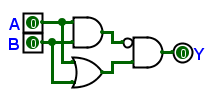
\includegraphics[width=\maxwidth{.95\linewidth}]{gfx/04_33}
	\caption{XOR Derived From AND/OR/NOT}
	\label{fig:04_33}
\end{figure}

While the Primary Operations are functionally complete, it is possible to define other functionally complete sets of operations. For example, using DeMorgan's Theorem, the set of \{\textsf{AND}, \textsf{NOT}\} is also functionally complete since the \textsf{OR}  operation can be defined as $ (A'B')' $. In fact, both \{\textsf{NAND}\} and \{NOR\} operations are functionally complete by themselves. As an example, the \textsf{NOT}  operation can be derived using only \textsf{NAND} gates: $ ( A | A ) $. Because all Boolean functions can be derived from either \textsf{NAND} or \textsf{NOR} operations, these are sometimes considered \emph{universal} operations and it is a common challenge for students to create some complex Boolean function using only one of these two types of operations.
\chapter{Boolean Expressions}\label{ch05}
\section{Introduction}

Electronic circuits that do not require any memory devices (like flip-flops or registers) are created using what is called ``Combinational Logic.'' These systems can be quite complex, but all outputs are determined solely by input signals that are processed through a series of logic gates. Combinational circuits can be reduced to a Boolean Algebra expression, though it may be quite complex; and that expression can be simplified using methods developed in this chapter and Chapter \ref{ch06}, \nameref{ch06}, page \pageref{ch06}, and Chapter \ref{ch07}, \nameref{ch07}, page \pageref{ch07}. Combinational circuits are covered in Chapter \ref{ch08}, \nameref{ch08}, page \pageref{ch08}.

In contrast, electronic circuits that require memory devices (like flip-flops or registers) use what is called ``Sequential Logic.'' Those circuits often include feedback loops, so the final output is determined by input signals plus the feedback loops that are processed through a series of logic gates. This makes sequential logic circuits much more complex than combinational and the simplification of those circuits is covered in Chapter \ref{ch09}, \nameref{ch09}, page \pageref{ch09}. 

Finally, most complex circuits include both combinational and sequential sub-circuits. In that case, the various sub-circuits would be independently simplified using appropriate methods. Several examples of these types of circuits are analyzed in Chapter \ref{ch10}, \nameref{ch10}, page \pageref{ch10}.

\section{Creating Boolean Expressions}

A circuit designer is often only given a written (or oral) description of a circuit and then asked to build that device. Too often, the designer may receive notes scribbled on the back of a dinner napkin, along with some verbal description of the desired output, and be expected to build a circuit to accomplish that task. Regardless of the form of the request, the process that the designer follows, in general, is: 

\begin{enumerate}
  \item \textsc{Write The Problem Statement}. The problem to be solved is written in a clear, concise statement. The better this statement is written the easier each of the following steps will be, so time spent polishing the problem statement is worthwhile. 
  
  \item \textsc{Construct A Truth Table}. Once the problem is clearly defined, the circuit designer constructs a truth table where all inputs/outputs are included. It is essential that all possible input combinations that lead to a \emph{True} output are identified. 
  
  \item \textsc{Write A Boolean Expression}. When the truth table is completed, it is easy to create a Boolean expression from that table as covered in Example \ref{05:subsec:example}. 
  
  \item \textsc{Simplify the Boolean Expression}. The expression should be simplified as much as possible, and that process is covered in this chapter, Chapter \ref{ch06}, \nameref{ch06}, page \pageref{ch06}, and Chapter \ref{ch07}, \nameref{ch07}, page \pageref{ch07}. 
  
  \item \textsc{Draw The Logic Diagram}. The logic diagram for a circuit is constructed from the simplified Boolean expression. 
  
  \item \textsc{Build The Circuit}. If desired, a physical circuit can be built using the logic diagram. 
\end{enumerate}

\subsection{Example}
\label{05:subsec:example}

A machine is to be programmed to help pack shipping boxes for the ABC Novelty Company. They are running a promotion so if a customer purchases any two of the following items, but not all three, a free poster will be added to the purchase: joy buzzer, fake blood, itching powder. Design the logic needed to add the poster to appropriate orders. 

\begin{enumerate}
  \item \textsc{Problem Statement}. The problem is already fairly well stated. A circuit is needed that will activate the ``drop poster'' machine when any two of three inputs (joy buzzer, fake blood, itching powder), but not all three, are \emph{True}. 

  \item \textsc{Truth Table}. Let $ J $ be the Joy Buzzer, $ B $ be the Fake Blood, and $ P $ be the Itching Powder; and let the truth table inputs be \emph{True} (or $ 1 $) when any of those items are present in the shipping box. Let the output $ D $ be for ``Drop Poster'' and when it is \emph{True} (or $ 1 $) then a poster will be dropped into the shipping box. The Truth table is illustrated in Table  \ref{05:tab:truth_table_for_example}.
  
  \begin{table}[H]
    \sffamily
    \newcommand{\head}[1]{\textcolor{white}{\textbf{#1}}}    
    \begin{center}
      \rowcolors{2}{gray!10}{white} % Color every other line a light gray
      \begin{tabular}{cccc} 
        \rowcolor{black!75}
        \multicolumn{3}{c}{\head{Inputs}} & \head{Output} \\
        J & B & P & D \\
        \hline
        0 & 0 & 0 & 0 \\
        0 & 0 & 1 & 0 \\
        0 & 1 & 0 & 0 \\
        0 & 1 & 1 & 1 \\
        1 & 0 & 0 & 0 \\
        1 & 0 & 1 & 1 \\
        1 & 1 & 0 & 1 \\
        1 & 1 & 1 & 0
      \end{tabular}
    \end{center}
    \caption{Truth Table for Example}
    \label{05:tab:truth_table_for_example}
  \end{table}
  
  \item \textsc{Write Boolean Expression}. According to the Truth Table, the poster will be dropped into the shipping box in only three cases (when output $ D $ is \emph{True}). Equation \ref{05:eq:example} was generated from the truth table. 
  
  \begin{align}
  \label{05:eq:example}
  BP + JP + JB &= D 
  \end{align}
  
  \item \textsc{Simplify Boolean Expression}. The Boolean expression for this problem is already as simple as possible so no further simplification is needed. 
  
  \item \textsc{Draw Logic Diagram}. Figure \ref{fig:05_01} was drawn from the switching equation.
  
	\begin{figure}[H]
		\centering
		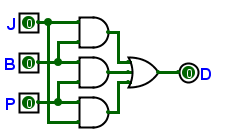
\includegraphics[width=\maxwidth{.95\linewidth}]{gfx/05_01}
		\caption{Logic Diagram From Switching Equation}
		\label{fig:05_01}
	\end{figure}
  
  \item \textsc{Build The Circuit}. This circuit could be built (or ``realized'') with three \textsf{AND}  gates and one 3-input \textsf{OR}  gate. 
  
\end{enumerate}

%***************************************************************************
% Section: Minterms and Maxterms
%***************************************************************************
\section{Minterms and Maxterms}
\label{05:sec:minterms_and_maxterms}

\subsection{Introduction}
\label{05:subsec:introduction_to_minterms_and_maxterms}

The solution to a Boolean equation is normally expressed in one of two formats: \ac{SOP} or \ac{POS}.

\subsection{Sum Of Products (SOP) Defined}
\label{05:subsec:sum_of_products_sop_defined}

Equation \ref{05:eq:sop_example} is an example of a \ac{SOP} expression. Notice that the expression describes four inputs ($ A $, $ B $, $ C $, $ D $) that are combined through two \textsf{AND} gates and then the output of those \textsf{AND} gates are combined through an \textsf{OR} gate. 

\begin{align}
  \label{05:eq:sop_example}
  (A'BC'D)+(AB'CD) &= Y
\end{align}

Each of the two terms in this expression is a \emph{minterm}. Minterms can be identified in a Boolean expression as a group of inputs joined by an \textsf{AND} gate and then two or more minterms are combined with an \textsf{OR} gate. \marginpar{Notice the inverting bubble on three of the AND gate inputs.}The circuit illustrated in Figure \ref{fig:05_02} would realize Equation \ref{05:eq:sop_example}.

\begin{figure}[H]
	\centering
	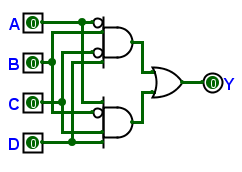
\includegraphics[width=\maxwidth{.95\linewidth}]{gfx/05_02}
	\caption{Logic Diagram For SOP Example}
	\label{fig:05_02}
\end{figure}

\subsection{Product of Sums (POS) Defined}
\label{05:subsec:product_of_sums_pos_defined}

Equation \ref{05:eq:pos_example} is an example of a \ac{POS} expression. Notice that the expression describes four inputs ($ A $, $ B $, $ C $, $ D $) that are combined through two \textsf{OR} gates and then the output of those \textsf{OR} gates are combined through an \textsf{AND} gate. 

\begin{align}
  \label{05:eq:pos_example}
  (A'+B+C+'D)(A+B'+C+D) &= Y
\end{align}

Each term in this expression is called a \emph{maxterm}. Maxterms can be identified in a Boolean expression as a group of inputs joined by an \textsf{OR} gate; and then two or more maxterms are combined with an \textsf{AND} gate. \marginpar{Notice the inverting bubble on three of the OR gate inputs.}The circuit illustrated in Figure \ref{fig:05_03} would realize Equation \ref{05:eq:pos_example}. 

\begin{figure}[H]
	\centering
	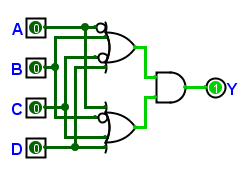
\includegraphics[width=\maxwidth{.95\linewidth}]{gfx/05_03}
	\caption{Logic Diagram For POS Example}
	\label{fig:05_03}
\end{figure}

\subsection{About Minterms}
\label{05:subsec:about_minterms}

A term that contains all of the input variables in one row of a truth table joined with an \textsf{AND} gate is called a minterm. Consider truth table \ref{05:tab:truth_table_for_first_minterm_example} which is for a circuit with three inputs ( $ A $,  $ B $, and  $ C $) and one output ( $ Q $).

\begin{table}[H]
  \sffamily
  \newcommand{\head}[1]{\textcolor{white}{\textbf{#1}}}    
  \begin{center}
    \rowcolors{2}{gray!10}{white} % Color every other line a light gray
    \begin{tabular}{ccc|cc} 
      \rowcolor{black!75}
      \multicolumn{3}{c}{\head{Inputs}} & \multicolumn{2}{c}{\head{Outputs}} \\
      A & B & C & Q & m\\
      \hline
      0 & 0 & 0 & 0 & 0 \\
      0 & 0 & 1 & 0 & 1 \\
      0 & 1 & 0 & 0 & 2 \\
      0 & 1 & 1 & 1 & 3 \\
      1 & 0 & 0 & 0 & 4 \\
      1 & 0 & 1 & 1 & 5 \\
      1 & 1 & 0 & 0 & 6 \\
      1 & 1 & 1 & 0 & 7 
    \end{tabular}
  \end{center}
  \caption{Truth Table for First Minterm Example}
  \label{05:tab:truth_table_for_first_minterm_example}
\end{table}

The circuit that is represented by this truth table would output a \emph{True} in only two cases, when the inputs are $ A'BC $ or $ AB'C $. Equation \ref{05:eq:first_minterm_example} describes this circuit.

\begin{align}
  \label{05:eq:first_minterm_example}
  (A'BC)+(AB'C) &= Q
\end{align}

The terms $ A'BC $ and $ AB'C $ are called \emph{minterms} and they contain every combination of input variables that outputs a \emph{True} when the three inputs are joined by an \textsf{AND} gate. Minterms are most often used to describe circuits that have fewer \emph{True} outputs than \emph{False} (that is, there are fewer $ 1 $'s than $ 0 $'s in the output column). In the example above, there are only two \emph{True} outputs with six \emph{False} outputs, so minterms describe the circuit most efficiently. 

Minterms are frequently abbreviated with a lower-case  $ m $ along with a subscript that indicates the decimal value of the variables. For example, $ A'BC $, the first of the \emph{True} outputs in the truth table above, has a binary value of $ 011 $, which is a decimal value of $ 3 $; thus, the minterm is $ m_3 $. The other minterm in this equation is $ m_5 $ since its binary value is $ 101 $, which equals decimal $ 5 $. It is possible to verbally describe the entire circuit as: $ m_3 $ \textsf{OR} $ m_5 $. For convenience, each of the minterm numbers are indicated in the last column of the truth table.

As another example, consider truth table \ref{05:tab:truth_table_for_second_minterm_example}.

\begin{table}[H]
  \sffamily
  \newcommand{\head}[1]{\textcolor{white}{\textbf{#1}}}    
  \begin{center}
    \rowcolors{2}{gray!10}{white} % Color every other line a light gray
    \begin{tabular}{cccc|cc} 
      \rowcolor{black!75}
      \multicolumn{4}{c}{\head{Inputs}} & \multicolumn{2}{c}{\head{Outputs}} \\
      A & B & C & D & Q & m \\
      \hline
      0 & 0 & 0 & 0 & 1 & 0 \\
      0 & 0 & 0 & 1 & 0 & 1 \\
      0 & 0 & 1 & 0 & 0 & 2 \\
      0 & 0 & 1 & 1 & 0 & 3 \\
      0 & 1 & 0 & 0 & 0 & 4 \\
      0 & 1 & 0 & 1 & 1 & 5 \\
      0 & 1 & 1 & 0 & 1 & 6 \\
      0 & 1 & 1 & 1 & 0 & 7 \\
      1 & 0 & 0 & 0 & 0 & 8 \\
      1 & 0 & 0 & 1 & 0 & 9 \\
      1 & 0 & 1 & 0 & 0 & 10 \\
      1 & 0 & 1 & 1 & 0 & 11 \\
      1 & 1 & 0 & 0 & 0 & 12 \\
      1 & 1 & 0 & 1 & 0 & 13 \\
      1 & 1 & 1 & 0 & 1 & 14 \\
      1 & 1 & 1 & 1 & 0 & 15 
    \end{tabular}
  \end{center}
  \caption{Truth Table for Second Minterm Example}
  \label{05:tab:truth_table_for_second_minterm_example}
\end{table}

Equation \ref{05:eq:second_minterm_example} describes this circuit because these are the rows where the output is \emph{True}.

\begin{align}
  \label{05:eq:second_minterm_example}
  (A'B'C'D')+(A'BC'D)+(A'BCD')+(ABCD') &= Q
\end{align}

These would be minterms $ m_0 $, $ m_5 $, $ m_6 $, and $ m_{14} $. Equation \ref{05:eq:sigma_notation_second_minterm_example} shows a commonly used, more compact way to express this result.

\begin{align}
  \label{05:eq:sigma_notation_second_minterm_example}
  \int(A,B,C,D) &= \sum(0,5,6,14)
\end{align}

Equation \ref{05:eq:sigma_notation_second_minterm_example} would read: ``For the function of inputs  $ A $,  $ B $,  $ C $, and  $ D $, the output is \emph{True} for minterms $ 0 $, $ 5 $, $ 6 $, and $ 14 $ when they are combined with an \textsf{OR}  gate.'' This format is called \emph{Sigma Notation}, and it is easy to derive the full Boolean equation from it by remembering that $ m_0 $ is $ 0000 $, or $ A'B'C'D' $; $ m_5 $ is $ 0101 $, or $ A'BC'D $; $ m_6 $ is $ 0110 $, or $ A'BCD' $; and $ m_{14} $ is $ 1110 $, or $ ABCD' $. Therefore, the Boolean equation can be quickly created from the Sigma Notation. 

A logic equation that is created using minterms is often called the \emph{Sum of Products} (or \emph{SOP}) since each term is composed of inputs \textsf{AND}ed together (``products'') and the terms are then joined by \textsf{OR} gates (``sums'').

\subsection{About Maxterms}
\label{05:subsec:about_maxterms}

A term that contains all of the input variables joined with an \textsf{OR} gate (``added together'') for a \emph{False} output is called a \emph{maxterm}. Consider Truth Table \ref{05:tab:truth_table_for_first_maxterm_example}, which has three inputs ( $ A $,  $ B $, and  $ C $) and one output ( $ Q $): 

\begin{table}[H]
  \sffamily
  \newcommand{\head}[1]{\textcolor{white}{\textbf{#1}}}    
  \begin{center}
    \rowcolors{2}{gray!10}{white} % Color every other line a light gray
    \begin{tabular}{ccc|cc} 
      \rowcolor{black!75}
      \multicolumn{3}{c}{\head{Inputs}} & \multicolumn{2}{c}{\head{Outputs}} \\
      A & B & C & Q & M \\
      \hline
      0 & 0 & 0 & 1 & 0 \\
      0 & 0 & 1 & 1 & 1 \\
      0 & 1 & 0 & 0 & 2 \\
      0 & 1 & 1 & 1 & 3 \\
      1 & 0 & 0 & 1 & 4 \\
      1 & 0 & 1 & 1 & 5 \\
      1 & 1 & 0 & 0 & 6 \\
      1 & 1 & 1 & 1 & 7 
    \end{tabular}
  \end{center}
  \caption{Truth Table for First Maxterm Example}
  \label{05:tab:truth_table_for_first_maxterm_example}
\end{table}

The circuit that is represented by this truth table would output a \emph{False} in only two cases. Since there are fewer \emph{False} outputs than \emph{True}, it is easier to create a Boolean equation that would generate the \emph{False} outputs. Because the equation describes the \emph{False} outputs, each term is built by \emph{complementing} the inputs for each of the \emph{False} output lines. After the output groups are defined, they are joined with an \textsf{AND} gate. Equation \ref{05:eq:first_maxterm_example} is the Boolean equation for Truth Table \ref{05:tab:truth_table_for_first_maxterm_example}.

\begin{align}
  \label{05:eq:first_maxterm_example}
  (A+B'+C)(A'+B'+C) &= Q
\end{align}

The terms $ A+B'+C $ and $ A'+B'+C $ are called $ maxterms $, and they contain the complement of the input variables for each of the \emph{False} output lines. Maxterms are most often used to describe circuits that have fewer \emph{False} outputs than \emph{True}. In Truth Table \ref{05:tab:truth_table_for_first_maxterm_example}, there are only two \emph{False} outputs with six \emph{True} outputs, so maxterms describe the circuit most efficiently.

Maxterms are frequently abbreviated with an upper-case  $ M $ along with a subscript that indicates the decimal value of the complements of the variables. For example, the complement of $ A+B'+C $, the first of the \emph{False} outputs in Truth Table \ref{05:tab:truth_table_for_first_maxterm_example}, is $ 010 $, which is a decimal value of 2; thus, the maxterm would be $ M_2 $. This can be confusing, but remember that the \emph{complements} of the inputs are used to form the expression. Thus, $ A+B'+C $ is $ 010 $, not $ 101 $. The other maxterm in this equation is $ M_6 $ since the binary value of its complement is $ 110 $, which equals decimal 6. It is possible to describe the entire circuit as a the product of two groups of maxterms: $ M_2 $ and $ M_6 $.

As another example, consider Truth Table \ref{05:tab:truth_table_for_second_maxterm_example}.

\begin{table}[H]
  \sffamily
  \newcommand{\head}[1]{\textcolor{white}{\textbf{#1}}}    
  \begin{center}
    \rowcolors{2}{gray!10}{white} % Color every other line a light gray
    \begin{tabular}{cccc|cc} 
      \rowcolor{black!75}
      \multicolumn{4}{c}{\head{Inputs}} & \multicolumn{2}{c}{\head{Outputs}} \\
      A & B & C & D & Q & M \\
      \hline
      0 & 0 & 0 & 0 & 1 & 0 \\
      0 & 0 & 0 & 1 & 1 & 1 \\
      0 & 0 & 1 & 0 & 1 & 2 \\
      0 & 0 & 1 & 1 & 0 & 3 \\
      0 & 1 & 0 & 0 & 1 & 4 \\
      0 & 1 & 0 & 1 & 1 & 5 \\
      0 & 1 & 1 & 0 & 1 & 6 \\
      0 & 1 & 1 & 1 & 1 & 7 \\
      1 & 0 & 0 & 0 & 1 & 8 \\
      1 & 0 & 0 & 1 & 0 & 9 \\
      1 & 0 & 1 & 0 & 1 & 10 \\
      1 & 0 & 1 & 1 & 1 & 11 \\
      1 & 1 & 0 & 0 & 0 & 12 \\
      1 & 1 & 0 & 1 & 1 & 13 \\
      1 & 1 & 1 & 0 & 1 & 14 \\
      1 & 1 & 1 & 1 & 1 & 15 
    \end{tabular}
  \end{center}
  \caption{Truth Table for Second Maxterm Example}
  \label{05:tab:truth_table_for_second_maxterm_example}
\end{table}

Equation \ref{05:eq:second_maxterm_example} describes this circuit.

\begin{align}
  \label{05:eq:second_maxterm_example}
  (A+B+C'+D')(A'+B+C+D')(A'+B'+C+D) &= Q
\end{align}

These would be maxterms $ M_3 $, $ M_9 $, and $ M_{12} $. Equation \ref{05:eq:pi_notation_second_maxterm_example} shows a commonly used, more compact way to express this result.

\begin{align}
  \label{05:eq:pi_notation_second_maxterm_example}
  \int(A,B,C,D) &= \prod(3,9,12)
\end{align}

Equation \ref{05:eq:pi_notation_second_maxterm_example} would read: ``For the function of  $ A $,  $ B $,  $ C $,  $ D $, the output is \emph{False} for maxterms $ 3 $, $ 9 $, and $ 12 $ when they are combined with an \textsf{AND}  gate.'' This format is called \emph{Pi Notation}, and it is easy to derive the Boolean equation from it. Remember that $ M_3 $ is $ 0011 $, or $ A+B+C'+D' $ (the complement of the inputs), $ M_9 $ is $ 1001 $, or $ A'+B+C+D' $, and $ M_{12} $ is $ 1100 $, or $ A'+B'+C+D $. The original equation can be quickly created from the Pi Notation. 

A logic equation that is created using maxterms is often called the \emph{Product of Sums} (or \emph{POS}) since each term is composed of inputs \textsf{OR} ed together (``sums'') and the terms are then joined by \textsf{AND}  gates (``products'').

\subsection{Minterm and Maxterm Relationships}
\label{05:subsec:minterm_and_maxterm_relationships}

The minterms and maxterms of a circuit have three interesting relationships: equivalence, duality, and inverse. To define and understand these terms, consider Truth Table \ref{05:tab:minterm_and_maxterm_relationships_truth_table} for some unspecified ``black box'' circuit: 

\begin{table}[H]
  \sffamily
  \newcommand{\head}[1]{\textcolor{white}{\textbf{#1}}}    
  \begin{center}
    \rowcolors{2}{gray!10}{white} % Color every other line a light gray
    \begin{tabular}{ccc|cc|cc} 
      \rowcolor{black!75}
      \multicolumn{3}{c}{\head{Inputs}} & \multicolumn{2}{c}{\head{Outputs}} & \multicolumn{2}{c}{\head{Terms}} \\
      A & B & C & Q & Q' & minterm & Maxterm \\
      \hline
      0 & 0 & 0 & 0 & 1 & $ A'B'C' $ ($ m_0 $) & $ A+B+C $    ($ M_0 $) \\
      0 & 0 & 1 & 1 & 0 & $ A'B'C $  ($ m_1 $) & $ A+B+C' $   ($ M_1 $) \\
      0 & 1 & 0 & 0 & 1 & $ A'BC' $  ($ m_2 $) & $ A+B'+C $   ($ M_2 $) \\
      0 & 1 & 1 & 0 & 1 & $ A'BC $   ($ m_3 $) & $ A+B'+C' $  ($ M_3 $) \\
      1 & 0 & 0 & 0 & 1 & $ AB'C' $  ($ m_4 $) & $ A'+B+C $   ($ M_4 $) \\
      1 & 0 & 1 & 1 & 0 & $ AB'C $   ($ m_5 $) & $ A'+B+C' $  ($ M_5 $) \\
      1 & 1 & 0 & 0 & 1 & $ ABC' $   ($ m_6 $) & $ A'+B'+C $  ($ M_6 $) \\
      1 & 1 & 1 & 1 & 0 & $ ABC $    ($ m_7 $) & $ A'+B'+C' $ ($ M_7 $) 
    \end{tabular}
  \end{center}
  \caption{Minterm and Maxterm Relationships}
  \label{05:tab:minterm_and_maxterm_relationships_truth_table}
\end{table}

\subsubsection{Equivalence}
\label{05:subsubsec:equivalence}

The minterms and the maxterms for a given circuit are considered equivalent ways to describe that circuit. For example, the circuit described by Truth Table \ref{05:tab:minterm_and_maxterm_relationships_truth_table} could be defined using minterms (Equation \ref{05:eq:sigma_notation_minterm_and_maxterm_equivalence}).

\begin{align}
  \label{05:eq:sigma_notation_minterm_and_maxterm_equivalence}
  \int(A,B,C) &= \sum(1,5,7)
\end{align}

However, that same circuit could also be defined using maxterms (Equation \ref{05:eq:pi_notation_minterm_and_maxterm_equivalence}).

\begin{align}
  \label{05:eq:pi_notation_minterm_and_maxterm_equivalence}
  \int(A,B,C) &= \prod(0,2,3,4,6)
\end{align}

These two functions describe the same circuit and are, consequently, equivalent. The \emph{Sigma Function} includes the terms $ 1 $, $ 5 $, and $ 7 $ while the \emph{Pi Function} includes all other terms in the truth table ($ 0 $, $ 2 $, $ 3 $, $ 4 $, and $ 6 $). To put it a slightly different way, the \emph{Sigma Function} describes the truth table rows where Q = $ 1 $ (minterms) while the \emph{Pi Function} describes the rows in the same truth table where Q =  $ 0 $ (maxterms). Therefore, Equation \ref{05:eq:minterm_and_maxterm_equivalence} can be derived.

\begin{align}
  \label{05:eq:minterm_and_maxterm_equivalence}
  \sum(1,5,7) &\equiv \prod(0,2,3,4,6)
\end{align}

\subsubsection{Duality}
\label{05:subsubsec:duality}

Each row in Truth Table \ref{05:tab:minterm_and_maxterm_relationships_truth_table} describes two terms that are considered duals. For example, minterm $ m_5 $ ($ AB'C $) and maxterm $ M_5 $ ($ A'+B+C' $) are duals. Terms that are duals are complements of each other ($ Q $ vs. $ Q' $) and the input variables are also complements of each other; moreover, the inputs for the three minterms are combined with an \textsf{AND}  while the maxterms are combined with an \textsf{OR}. The output of the circuit described by Truth Table \ref{05:tab:minterm_and_maxterm_relationships_truth_table} could be defined using minterms (Equation \ref{05:eq:q_output_dual}).

\begin{align}
  \label{05:eq:q_output_dual}
  Q &= \sum(1,5,7)
\end{align}

The dual of the circuit would be defined by using the maxterms for the same output rows. However, those rows are the \emph{complement} of the circuit (Equation \ref{05:eq:q_not_output_dual}).

\begin{align}
  \label{05:eq:q_not_output_dual}
  Q' &= \prod(1,5,7)
\end{align}

This leads to the conclusion that the complement of a \textit{Sigma Function} is the \textit{Pi Function} with the same inputs, as in Equation \ref{05:eq:dual} (the overline was used to emphasize the the fact that the \textit{PI Function} is complemented).

\begin{align}
  \label{05:eq:dual}
  \sum(1,5,7) &= \overline{\prod(1,5,7)}
\end{align}


\subsubsection{Inverse}
\label{05:subsubsec:inverse}

The complement of a function yields the opposite output. For example the following functions are inverses because one defines $ Q $ while the other defines $ Q' $ using only minterms of the same circuit (or truth table).

\begin{align}
  \label{05:eq:q_output_inverse}
  Q &= \sum(1,5,7)
\end{align}

\begin{align}
  \label{05:eq:q_not_output_inverse}
  Q' &= \sum(0,2,3,4,6)
\end{align}

\subsubsection{Summary}
\label{05:subsubsec:summary_minterm_and_maxterm_relationships}

These three relationships are summarized in the following table. Imagine a circuit with two or more inputs and an output of  $ Q $. Table \ref{05:tab:minterm_and_maxterm_relationships} summarizes the various relationships in the Truth Table for that circuit.

\begin{table}[H]
  \sffamily
  \begin{center}
    \begin{tabular}{|l|l|} 
      \hline
      Minterms where Q is 1 & Minterms where Q' is 1 \\
      \hline
      Maxterms where Q is 1 & Maxterms where Q' is 1 \\
      \hline
    \end{tabular}
  \end{center}
  \caption{Minterm-Maxterm Relationships}
  \label{05:tab:minterm_and_maxterm_relationships}
\end{table}

The adjacent items in a single column are equivalent (that is,  $ Q $ Minterms are equivalent to  $ Q $ Maxterms), items that are diagonal are duals ( $ Q $ Minterms and  $ Q' $ Maxterms are duals), and items that are adjacent in a single row are inverses ( $ Q $ Minterms and  $ Q' $ Minterms are inverses). 

\subsection{Sum of Products Example}
\label{05:subsubsec:sum_of_products_example}

\subsubsection{Given}
\label{05:subsubsec:given_sop_example}

A ``vote-counter'' machine is designed to turn on a light if any two or more of three inputs are \emph{True}. Create a circuit to realize this machine. 

\subsubsection{Truth Table}
\label{05:subsubsec:truth_table_sop_example}

When realizing a circuit from a verbal description, the best place to start is constructing a truth table. This will make the Boolean expression easy to write and then make the circuit easy to realize. For the ``vote-counter'' problem, start by defining variables for the truth table: Inputs  $ A $,  $ B $,  $ C $ and Output  $ Q $. 

Next, construct the truth table by identifying columns for each of the three input variables and then indicate the output for every possible input condition (Table \ref{05:tab:truth_table_for_sop_example}).

\begin{table}[H]
  \sffamily
  \newcommand{\head}[1]{\textcolor{white}{\textbf{#1}}}    
  \begin{center}
    \rowcolors{2}{gray!10}{white} % Color every other line a light gray
    \begin{tabular}{ccc|cc} 
      \rowcolor{black!75}
      \multicolumn{3}{c}{\head{Inputs}} & \multicolumn{2}{c}{\head{Outputs}} \\
      A & B & C & Q & m\\
      \hline
      0 & 0 & 0 & 0 & 0 \\
      0 & 0 & 1 & 0 & 1 \\
      0 & 1 & 0 & 0 & 2 \\
      0 & 1 & 1 & 1 & 3 \\
      1 & 0 & 0 & 0 & 4 \\
      1 & 0 & 1 & 1 & 5 \\
      1 & 1 & 0 & 1 & 6 \\
      1 & 1 & 1 & 1 & 7 
    \end{tabular}
  \end{center}
  \caption{Truth Table for SOP Example}
  \label{05:tab:truth_table_for_sop_example}
\end{table}

\subsubsection{Boolean Equation}
\label{05:subsubsec:boolean_equation_sop_example}

In a truth table, if there are fewer \emph{True} outputs than \emph{False}, then it is easiest to construct a Sum-of-Products equation. In that case, a Boolean expression can be derived by creating the minterms for all \emph{True} outputs and combining those minterms with \textsf{OR}  gates. Equation \ref{05:eq:sigma_notation_sop_example} is the \emph{Sigma Function} of this circuit.

\begin{align}
  \label{05:eq:sigma_notation_sop_example}
  \int(A,B,C) &= \sum(3,5,6,7)
\end{align}

% Pull Quote - Marginal Note - Sidebar
\marginpar{It may be possible to simplify the Boolean expression, but that process is covered elsewhere in this book.}

At this point, a circuit could be created with four 3-input \textsf{AND}  gates combined into one 4-input \textsf{OR}  gate.

\subsection{Product of Sums Example}
\label{05:subsubsec:product_of_sums_example}

\subsubsection{Given}
\label{05:subsubsec:given_pos_example}

A local supply company is designing a machine to sort packages for shipping. All packages go to the post office \emph{except} packages going to the local ZIP code containing chemicals (they are shipped by courier) and packages going to a distant ZIP code containing only perishables (they are shipped via air freight).

\subsubsection{Truth Table}
\label{05:subsubsec:truth_table_pos_example}

When realizing a circuit from a verbal description, the best place to start is constructing a truth table. This will make the Boolean expression easy to write and then make the circuit easy to realize. For the sorting machine problem, start by defining variables for the truth table: 

\begin{itemize}
  \item Ship via post office (the Output):  $ O $ is \emph{True} if ship by Post Office
  \item Zip Code:  $ Z $ is \emph{True} if the zip code is local
  \item Chemicals:  $ C $ is \emph{True} if the package contains chemicals
  \item Perishable:  $ P $ is \emph{True} if the package contains perishables
\end{itemize}

Next, construct the truth table by identifying columns for each of the three input variables and then indicate the output for every possible input condition (Table \ref{05:tab:truth_table_for_sop_example}).

\begin{table}[H]
  \sffamily
  \newcommand{\head}[1]{\textcolor{white}{\textbf{#1}}}    
  \begin{center}
    \rowcolors{2}{gray!10}{white} % Color every other line a light gray
    \begin{tabular}{ccc|cc} 
      \rowcolor{black!75}
      \multicolumn{3}{c}{\head{Inputs}} & \multicolumn{2}{c}{\head{Outputs}} \\
      Z & C & P & O & M \\
      \hline
      0 & 0 & 0 & 1 & 0 \\
      0 & 0 & 1 & 0 & 1 \\
      0 & 1 & 0 & 1 & 2 \\
      0 & 1 & 1 & 0 & 3 \\
      1 & 0 & 0 & 1 & 4 \\
      1 & 0 & 1 & 1 & 5 \\
      1 & 1 & 0 & 0 & 6 \\
      1 & 1 & 1 & 0 & 7 
    \end{tabular}
  \end{center}
  \caption{Truth Table for POS Example}
  \label{05:tab:truth_table_for_pos_example}
\end{table}

\subsubsection{Boolean Equation}
\label{05:subsubsec:boolean_equation_pos_example}

In the truth table, if there are fewer \emph{False} outputs than \emph{True} then it is easiest to construct a Products-of-Sums equation. In that case, a Boolean expression can be derived by creating the maxterms for all \emph{False} outputs and combining the complement those maxterms with \textsf{AND}  gates. Equation \ref{05:eq:pi_notation_pos_example} is the \emph{Pi Expression} of this circuit.

\begin{align}
  \label{05:eq:pi_notation_pos_example}
  \int(Z,C,P) &= \prod(1,3,6,7)
\end{align}

% Pull Quote - Marginal Note - Sidebar
\marginpar{It may be possible to simplify the Boolean expression, but that process is covered elsewhere in this book.}

At this point, a circuit could be created with four 3-input \textsf{OR}  gates combined into one 4-input \textsf{AND}  gate.

\subsection{Summary}
\label{05:subsubsec:summary_minterms_and_maxterms}

\ac{SOP} Boolean expressions may be generated from truth tables quite easily, by determining which rows of the table have an output of \emph{True}, writing one minterm for each of those rows, and then summing all of the minterms. The resulting expression will lend itself well to implementation as a set of \textsf{AND} gates (products) feeding into a single \textsf{OR} gate (sum). 

\ac{POS} Boolean expressions may be generated from truth tables quite easily, by determining which rows of the table have an output of \emph{False}, writing one maxterm for each of those rows, and then multiplying all of the maxterms. The resulting expression will lend itself well to implementation as a set of \textsf{OR} gates (sums) feeding into a single \textsf{AND} gate (product). 

%***************************************************************************
% Section: Canonical Form
%***************************************************************************
\section{Canonical Form}
\label{05:sec:canonical_form}

\subsection{Introduction}
\label{05:subsec:introduction_to_canonical_form}

The word ``canonical'' simply means ``standard'' and it is used throughout mathematics and science to denote some standard form for equations. In digital electronics, Boolean equations are considered to be in canonical form when each of the terms in the equation includes all of the possible inputs and those terms appear in the same order as in the truth table. Using the canonical form is important when simplifying a Boolean equation. For example, imagine the solution to a given problem generated table \ref{05:tab:canonical_example_truth_table}.

\begin{table}[H]
  \sffamily
  \newcommand{\head}[1]{\textcolor{white}{\textbf{#1}}}    
  \begin{center}
    \rowcolors{2}{gray!10}{white} % Color every other line a light gray
    \begin{tabular}{ccc|cc} 
      \rowcolor{black!75}
      \multicolumn{3}{c}{\head{Inputs}} & \multicolumn{2}{c}{\head{Outputs}} \\
      A & B & C & Q & m \\
      \hline
      0 & 0 & 0 & 0 & 0 \\
      0 & 0 & 1 & 1 & 1 \\
      0 & 1 & 0 & 0 & 2 \\
      0 & 1 & 1 & 1 & 3 \\
      1 & 0 & 0 & 0 & 4 \\
      1 & 0 & 1 & 0 & 5 \\
      1 & 1 & 0 & 0 & 6 \\
      1 & 1 & 1 & 1 & 7 
    \end{tabular}
  \end{center}
  \caption{Canonical Example Truth Table}
  \label{05:tab:canonical_example_truth_table}
\end{table}

Minterm equation \ref{05:eq:canonical_example} is derived from the truth table and is presented in canonical form. Notice that each term includes all possible inputs ( $ A $,  $ B $, and  $ C $), and that the terms are in the same order as they appear in the truth table. 

\begin{align}
  \label{05:eq:canonical_example}
  (A'B'C)+(A'BC)+(ABC) &= Q
\end{align}

Frequently, though, a Boolean equation is expressed in standard form, which is not the same as canonical form. Standard form means that some of the terms have been simplified and not all of the inputs will appear in all of the terms. For example, consider Equation \ref{05:eq:standard_form_example}, which is the solution for a 4-input circuit.

\begin{align}
  \label{05:eq:standard_form_example}
  (A'C)+(B'CD) &= Q
\end{align}

This equation is in standard form so the first term, $ A'C $, does not include inputs  $ B $ or  $ D $ and the second term, $ B'CD $, does not include input  $ A $. However, all inputs must be present in every term for an equation to be in canonical form.

Building a truth table for an equation in standard form raises an important question. Consider the truth table for Equation \ref{05:eq:standard_form_example}.

\begin{table}[H]
  \sffamily
  \newcommand{\head}[1]{\textcolor{white}{\textbf{#1}}}    
  \begin{center}
    \rowcolors{2}{gray!10}{white} % Color every other line a light gray
    \begin{tabular}{cccc|cc} 
      \rowcolor{black!75}
      \multicolumn{4}{c}{\head{Inputs}} & \multicolumn{2}{c}{\head{Outputs}} \\
      A & B & C & D & Q & m \\
      \hline
      0 & 0 & 0 & 0 & 0 & 0 \\
      0 & 0 & 0 & 1 & 0 & 1 \\
      0 & 0 & 1 & 0 & 0 & 2 \\
      0 & 0 & 1 & 1 & ? & 3 \\
      0 & 1 & 0 & 0 & 0 & 4 \\
      0 & 1 & 0 & 1 & 0 & 5 \\
      0 & 1 & 1 & 0 & 0 & 6 \\
      0 & 1 & 1 & 1 & 0 & 7 \\
      1 & 0 & 0 & 0 & 0 & 8 \\
      1 & 0 & 0 & 1 & 0 & 9 \\
      1 & 0 & 1 & 0 & 0 & 10 \\
      1 & 0 & 1 & 1 & ? & 11 \\
      1 & 1 & 0 & 0 & 0 & 12 \\
      1 & 1 & 0 & 1 & 0 & 13 \\
      1 & 1 & 1 & 0 & 0 & 14 \\
      1 & 1 & 1 & 1 & 0 & 15 
    \end{tabular}
  \end{center}
  \caption{Truth Table for Standard Form Equation}
  \label{05:tab:truth_table_for_standard_form_equation}
\end{table}

In what row would $ B'CD $, the second term in Equation \ref{05:eq:standard_form_example}, be placed? $ B'CD $ is $ 011 $ (in binary), but since the $ A $ term is missing would it be a $ 0 $ or $ 1 $; in other words, would $ B'CD $ generate an output of $ 1 $ for row $ 0011\;(m_3)$ or $ 1011\;(m_{11})$? (The output for these two rows are marked with a question mark in Table \ref{05:tab:truth_table_for_standard_form_equation}.) In fact, the output for \emph{both} of these rows must be considered \emph{True} in order to ensure that all possible combinations of input are covered. Thus, the final equation for this circuit must include at least these two terms: $ (A'B'CD) + (AB'CD) $. In the same way, the term $ A'C $ means that the output is \emph{True} for $ m_2 $, $ m_3 $, $ m_6 $, and $ m_7 $ since input $ A'C $ is \emph{True} and any minterm that contains those two value is also considered \emph{True}. Thus, the final equation for this circuit must include at least these four terms: $ (A'B'CD') + (A'B'CD) + (A'BCD') + (A'BCD) $.

\subsection{Converting Terms Missing One Variable}
\label{05:subsec:converting_terms_missing_one_variable}

To change a standard Boolean expression that is missing one input term into a canonical Boolean expression, insert both \emph{True} and \emph{False} for the missing term into the original standard expression. As an example, consider the term $ B'CD $. Since term $ A $ is missing, both $ A $ and $ A' $ must be included in the converted canonical expression. Equation \ref{05:eq:canonical_expanding_3-variable_term} proves that $ B'CD $ can be expanded to include both possible values for $ A $ by using the Adjacency Property (page \pageref{BF:subsec:adjacency_property}).

\begin{align}
  \label{05:eq:canonical_expanding_3-variable_term}
  (B'CD) \rightarrow (AB'CD)+(A'B'CD)
\end{align}

A term that is missing one input variable will expand into two terms that include all variables. For example, in a system with four input variables (as above), any standard term with only three variables will expand to a canonical expression containing two groups of four variables. 

Expanding a standard term that is missing one variable can also be done with a truth table. To do that, fill in an output of $ 1 $ for every line where the \emph{True} inputs are found while ignoring all missing variables. As an example, consider Truth Table \ref{05:tab:truth_table_for_standard_form_equation} where the outputs for $ m_3 $ and $ m_11 $ are marked with a question mark. However, the output for both of these lines should be marked as \emph{True} because  $ B'CD $ is \emph{True} (input $ A $ is ignored). Then, those two minterms lead to the Boolean expression $ AB'CD + A'B'CD $.

\subsection{Converting Terms Missing Two Variables}
\label{05:subsec:converting_terms_missing_two_variables}

It is easiest to expand a standard expression that is missing two terms by first inserting one of the missing variables and then inserting the other missing variable in two distinct steps. The process for inserting a single missing variable is found in Section \ref{05:subsec:converting_terms_missing_one_variable}. Consider the term $ A'C $ in a four-variable system. It is missing both the $ B $ and $ D $ variables. To expand that term to its canonical form, start by inserting either of the two missing variables. For example, Equation \ref{05:eq:canonical_expanding_2-variable_term_step_one} illustrates entering $ B $ and $ B' $ into the expression.

\begin{align}
  \label{05:eq:canonical_expanding_2-variable_term_step_one}
  (A'C) &\rightarrow (A'BC)+(A'B'C)
\end{align}

Then, Equation \ref{05:eq:canonical_expanding_2-variable_term_step_two} illustrates inserting $ D $ and $ D' $ into the expression.

\begin{align}
  \label{05:eq:canonical_expanding_2-variable_term_step_two}
  (A'BC) &\rightarrow (A'BCD)+(A'BCD') \\
  \nonumber
  (A'B'C) &\rightarrow (A'B'CD)+(A'B'CD')
\end{align}

In the end, $ A'C $ expands to Equation \ref{05:eq:canonical_expanding_2-variable_term_step_three}:

\begin{align}
  \label{05:eq:canonical_expanding_2-variable_term_step_three}
  (A'C) \rightarrow &(A'BCD) + (A'BCD') \\
  \nonumber
  &+ (A'B'CD) + (A'B'CD')
\end{align}

Thus, in a four-variable system, any standard term with only two variables will expand to a canonical expression with four groups of four variables.

Expanding a standard term that is missing two variables can also be done with a truth table. To do that, fill in an output of $ 1 $ for every line where the \emph{True} inputs are found while ignoring all missing variables. As an example, consider a Table \ref{05:tab:truth_table_for_expression_with_missing_variables}, where $ A'C $ is marked as \emph{True}:

\begin{table}[H]
  \sffamily
  \newcommand{\head}[1]{\textcolor{white}{\textbf{#1}}}    
  \begin{center}
    \rowcolors{2}{gray!10}{white} % Color every other line a light gray
    \begin{tabular}{cccc|cc} 
      \rowcolor{black!75}
      \multicolumn{4}{c}{\head{Inputs}} & \multicolumn{2}{c}{\head{Outputs}} \\
      A & B & C & D & Q & m \\
      \hline
      0 & 0 & 0 & 0 & 0 & 0 \\
      0 & 0 & 0 & 1 & 0 & 1 \\
      0 & 0 & 1 & 0 & 1 & 2 \\
      0 & 0 & 1 & 1 & 1 & 3 \\
      0 & 1 & 0 & 0 & 0 & 4 \\
      0 & 1 & 0 & 1 & 0 & 5 \\
      0 & 1 & 1 & 0 & 1 & 6 \\
      0 & 1 & 1 & 1 & 1 & 7 \\
      1 & 0 & 0 & 0 & 0 & 8 \\
      1 & 0 & 0 & 1 & 0 & 9 \\
      1 & 0 & 1 & 0 & 0 & 10 \\
      1 & 0 & 1 & 1 & 0 & 11 \\
      1 & 1 & 0 & 0 & 0 & 12 \\
      1 & 1 & 0 & 1 & 0 & 13 \\
      1 & 1 & 1 & 0 & 0 & 14 \\
      1 & 1 & 1 & 1 & 0 & 15 
    \end{tabular}
  \end{center}
  \caption{Truth Table for Standard Form Equation}
  \label{05:tab:truth_table_for_expression_with_missing_variables}
\end{table}

Notice that outputs for $ m_2 $, $ m_3 $, $ m_6 $, and $ m_7 $ are \emph{True} because for each of those minterms $ A'C $ is \emph{True} (inputs $ B $ and $ D $ are ignored). Then, those four minterms lead to the Boolean expression $ A'B'CD'+A'B'CD+A'BCD'+A'BCD $.

\subsection{Summary}
\label{05:subsec:summary_of_canonical_forms}

This discussion started with Equation \ref{05:eq:standard_form_example_repeated}, which is in standard form.

\begin{align}
  \label{05:eq:standard_form_example_repeated}
  (A'C)+(B'CD) &= Q
\end{align}

After expanding both terms, Equation \ref{05:eq:canonical_form_summary_equation_not_simplified} is generated.

\begin{align}
  \label{05:eq:canonical_form_summary_equation_not_simplified}
  &(A'BCD)+(A'BCD')+(A'B'CD) \\
  \nonumber
  +&(A'B'CD')+(AB'CD)+(A'B'CD) = Q
\end{align}

Notice, though, that the term $ A'B'CD $ appears two times, so one of those can be eliminated by the Idempotence property (page \pageref{BF:subsec:idempotence}), leaving Equation \ref{05:eq:canonical_form_summary_equation_simplified}.

\begin{align}
  \label{05:eq:canonical_form_summary_equation_simplified}
  &(A'BCD)+(A'BCD') \\
  \nonumber
  +&(A'B'CD')+(AB'CD)+(A'B'CD) = Q
\end{align}

To put the equation in canonical form, which is important for simplification; all that remains is to rearrange the terms so they are in the same order as they would appear in a truth table, which results in Equation \ref{05:eq:canonical_form_summary_equation_final}.

\begin{align}
  \label{05:eq:canonical_form_summary_equation_final}
  &(A'B'CD')+(A'B'CD) \\
  \nonumber
  +&(A'BCD')+(A'BCD)+(AB'CD) = Q
\end{align}

\subsection{Practice Problems}
\label{05:subsec:practice_with_canonical_forms}

\marginpar{Parenthesis were not used in order to save space; however, the variable groups are evident.}

\begin{table}[H]
  \sffamily
  \begin{center}
    \begin{tabular}{c c p{6cm} }
      \multirow{2}{*}{\textbf{1}} 
        & Standard (A,B,C) & $ A'B+C+AB' $ \\
        & \cellcolor{gray!10} Cannonical 
        & \cellcolor{gray!10} $ A'B'C+A'BC'+A'BC+AB'C'+AB'C+ABC $ \\
      \hline
      \multirow{2}{*}{\textbf{2}} 
      & Standard (A,B,C,D) & $ A'BC+B'D $ \\
      & \cellcolor{gray!10} Cannonical 
      & \cellcolor{gray!10} $ A'B'C'D'+A'B'CD'+A'BCD'+A'BCD+AB'C'D'+AB'CD' $ \\
      \hline
      \multirow{2}{*}{\textbf{3}} 
      & Standard (A,B,C,D) & $ A'+D $ \\
      & \cellcolor{gray!10} Cannonical 
      & \cellcolor{gray!10} $ A'B'C'D'+A'B'C'D+A'B'CD'+A'B'CD+A'BC'D'       +A'BC'D+A'BCD'+A'BCD+AB'C'D+AB'CD+ABC'D+ABCD $ \\
      \hline
      \multirow{2}{*}{\textbf{4}} 
      & Standard (A,B,C) & $ A(B'+C) $ \\
      & \cellcolor{gray!10} Cannonical 
      & \cellcolor{gray!10} $ AB'C'+AB'C+ABC $ \\
    \end{tabular}
  \end{center}
  \caption{Canonical Form Practice Problems}
  \label{05:tab:canonical_form_practice_problems}
\end{table}

%***************************************************************************
% Section: Simplification Using Algebraic Methods
%***************************************************************************
\section{Simplification Using Algebraic Methods}
\label{05:sec:simplification_using_algebraic_methods}

\subsection{Introduction}
\label{05:subsec:introduction_to_algebraic_methods}

One method of simplifying a Boolean equation is to use common algebraic processes. It is possible to reduce an equation step-by-step using the various properties of Boolean algebra in the same way that real-number equations can be simplified. 

\subsection{Starting From a Circuit}
\label{05:subsec:starting_from_a_circuit}

Occasionally, the circuit designer is faced with an existing circuit and must attempt to simplify it. In that case, the first step is to find the Boolean equation for the circuit and then simplify that equation. 

\subsubsection{Generate a Boolean Equation}
\label{05:subsubsec:generate_a_boolean_equation}

In the circuit illustrated in Figure \ref{fig:05_04}, the  $ A $,  $ B $, and  $ C $ input signals are assumed to be provided from switches, sensors, or perhaps other sub-circuits. Where these signals originate is of no concern in the task of gate reduction.

\begin{figure}[H]
	\centering
	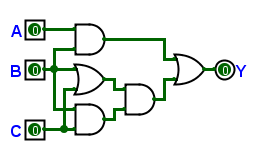
\includegraphics[width=\maxwidth{.95\linewidth}]{gfx/05_04}
	\caption{Example Circuit}
	\label{fig:05_04}
\end{figure}

To generate the Boolean equation for a circuit, write the output of each gate as determined by the input signals and type of gate, working from the inputs to the final output. Figure \ref{fig:05_05} illustrates the result of this process.

\begin{figure}[H]
	\centering
	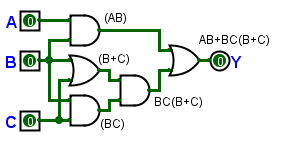
\includegraphics[width=\maxwidth{.95\linewidth}]{gfx/05_05}
	\caption{Example Circuit With Gate Outputs}
	\label{fig:05_05}
\end{figure}

This process leads to Equation \ref{05:eq:equation_from_circuit}.

\begin{align}
  \label{05:eq:equation_from_circuit}
  AB+BC(B+C) &= Y
\end{align}

\subsection{Starting From a Boolean Equation}
\label{05:subsec:starting_from_a_boolean_equation}

If a logic circuit's function is expressed as a Boolean equation, then algebraic methods can be applied to reduce the number of logic gates, resulting in a circuit that performs the same function with fewer components. As an example, Equation \ref{05:soln:equation_to_simplify_one_solution} simplifies the circuit found in Figure \ref{05:fig:circuit_with_boolean_expression}. 

\begin{align}
\label{05:soln:equation_to_simplify_one_solution}
  AB+BC(B+C) && \text{Original Expression} \\
  \nonumber
  AB+BBC+BCC && \text{Distribute BC} \\
  \nonumber
  AB+BC+BC && \text{Idempotence: BB=B and CC=C} \\
  \nonumber
  AB+BC && \text{Idempotence: BC+BC=BC} \\
  \nonumber
  B(A+C) && \text{Factor} 
\end{align}

The final expression, $ B(A + C) $, requires only two gates, and is much simpler than the original, yet performs the same function. Such component reduction results in higher operating speed (less gate propagation delay), less power consumption, less cost to manufacture, and greater reliability. 

As a second example, consider Equation \ref{05:eq:equation_to_simplify_two}.

\begin{align}
  \label{05:eq:equation_to_simplify_two}
  A+AB &= Y
\end{align}

This is simplified below.

\begin{align}
\label{05:soln:equation_to_simplify_two}
  A+AB && \text{Original Expression} \\
  \nonumber
  A(1+B) && \text{Factor} \\
  \nonumber
  A(1) && \text{Annihilation (1+B=1)} \\
  \nonumber
  A && \text{Identity A1=A}
\end{align}

The original expression, $ A+AB $ has been reduced to  $ A $ so the original circuit could be replaced by a wire directly from input  $ A $ to output  $ Y $. Equation \ref{05:eq:equation_to_simplify_three} looks similar to Equation \ref{05:eq:equation_to_simplify_two}, but is quite different and requires a more clever simplification.

\begin{align}
  \label{05:eq:equation_to_simplify_three}
  A+A'B &= Y
\end{align}

This is simplified below.

\begin{align}
  \label{05:soln:equation_to_simplify_three}
  A+A'B && \text{Original Expression} \\
  \nonumber
  A+AB+A'B && \text{Expand A to A+AB (Absorption)} \\
  \nonumber
  A+B(A+A') && \text{Factor B out of the last two terms} \\
  \nonumber
  A+B(1) && \text{Complement Property} \\
  \nonumber
  A+B && \text{Identityt: B(1)=B} 
\end{align}

Note how the Absorption Property ($ A + AB = A $) is used to ``un-simplify'' the first  $ A $ term, changing  $ A $ into $ A + AB $. While this may seem like a backward step, it ultimately helped to reduce the expression to something simpler. Sometimes ``backward'' steps must be taken to achieve the most elegant solution. Knowing when to take such a step is part of the art of algebra. 

As another example, simplify this \ac{POS} expression equation: 

\begin{align}
  \label{05:eq:equation_to_simplify_four}
  (A+B)(A+C) &= Y
\end{align}

This is simplified below.

\begin{align}
  \label{05:soln:equation_to_simplify_four}
  (A+B)(A+C) && \text{Original Expression} \\
  \nonumber
  AA+AC+AB+BC && \text{Distribute A+B} \\
  \nonumber
  A+AC+AB+BC && \text{Idempotence: AA=A} \\
  \nonumber
  A+AB+BC && \text{Absorption: A+AC=A} \\
  \nonumber
  A+BC && \text{Absorption: A+AB=A}
\end{align}

In each of the examples in this section, a Boolean expression was simplified using algebraic methods, which led to a reduction in the number of gates needed and made the final circuit more economical to construct and reliable to operate. 

\subsection{Practice Problems}
\label{05:subsec:practice_problems_for_simplifying_with_algebra}

Table \ref{05:tab:simplifying_boolean_expressions} shows a Boolean expression on the left and its simplified version on the right. This is provided for practice in simplifying expressions using algebraic methods. 

\begin{table}[H]
  \sffamily
  \newcommand{\head}[1]{\textcolor{white}{\textbf{#1}}}    
  \begin{center}
    \rowcolors{2}{gray!10}{white} % Color every other line a light gray
    \begin{tabular}{cc}
      \rowcolor{black!75}
      \head{Original Expression} & \head{Simplified} \\
      $ A(A'+B) $ & $ AB $ \\
      $ A+A'B $ & $ A+B $ \\
      $ (A+B)(A+B') $ & $ A $ \\
      $ AB+A'C+BC $ & $ AB+A'C $ \\
    \end{tabular}
  \end{center}
  \caption{Simplifying Boolean Expressions}
  \label{05:tab:simplifying_boolean_expressions}
\end{table}
% Chapter: Karnaugh maps
\chapter{Karnaugh maps}\label{ch06}

\begin{tcolorbox}[colback=blue!5!white,colframe=blue!75!black]
	% Upper half of box: my "title" area
	\textcolor{blue}{\textbf{What to Expect}}
	% Lower half of the box: the content
	\tcblower
	This chapter introduces a graphic tool that is used to simplify Boolean expressions: Karnaugh Maps. A Karnaugh Map plots a circuit's output on a matrix and then use a straightforward technique to combine those outputs to create a simplified circuit. This chapter includes the following topics.
	
	\begin{itemize}
		\item Drawing a Karnaugh map for two/three/four variables
		\item Simplifying groups of two/four/eight/sixteen
		\item Simplifying a Karnaugh Map that includes overlapping groups
		\item Wrapping groups ``around the edge'' of a Karnaugh Map
		\item Analyzing circuits that include ``Don't Care'' terms
		\item Applying Reed-Muller logic to a Karnaugh Map
	\end{itemize}
	
\end{tcolorbox}

\section{Introduction}

% Pull Quote - Marginal Note - Sidebar
\marginpar{Maurice Karnaugh developed this process at Bell Labs in 1953 while designing switching circuits for landline telephones.}

A Karnaugh map, like Boolean algebra, is a tool used to simplify a digital circuit. Keep in mind that ``simplify'' means reducing the number of gates and inputs for each gate and as components are eliminated, not only does the manufacturing cost go down, but the circuit becomes simpler, more stable, and more energy efficient. 

In general, using Boolean Algebra is the easiest way to simplify a circuit involving one to three input variables. For four input variables, Boolean algebra becomes tedious and Karnaugh maps are both faster and easier (and are less prone to error). However, Karnaugh maps become rather complex with five input variables and are generally too difficult to use above six variables (with more than four input variables, a Karnaugh map uses multiple dimensions that become very challenging to manipulate). For five or more input variables, circuit simplification should be done by Quine-McClusky methods  (page \pageref{ASM:sec:quine-mccluskey_simplification_method}) or the use of \gls{cat} (page \pageref{ASM:sec:automated_tools}).

In theory, any of the methods will work for any number of variables; however, as a practical matter, the guidelines presented in Table \ref{KM:tab:circuit_simplification_methods} work well. Normally, there is no need to resort to \gls{cat} to simplify a simple equation involving two or three variables since it is much quickly to use either Boolean Algebra or Karnaugh maps. However, for more complex input/output combinations, then \gls{cat} become essential to both speed the process and improve accuracy. 

\begin{table}[H]
  \sffamily
  \newcommand{\head}[1]{\textcolor{white}{\textbf{#1}}}    
  \begin{center}
    \rowcolors{2}{gray!10}{white} % Color every other line a light gray
    \begin{tabular}{ccccc} 
      \rowcolor{black!75}
      \head{Variables} & \head{Algebra} & \head{K-Map} & \head{Quine-McClusky} & \head{CAT} \\
      1-2 & X &   &   &   \\
      3   & X & X &   &   \\
      4   & X & X &   &   \\
      5-6 &   & X & X &   \\
      7-8 &   &   & X & X \\
      >8  &   &   &   & X
    \end{tabular}
  \end{center}
  \caption{Circuit Simplification Methods}
  \label{KM:tab:circuit_simplification_methods}
\end{table}

\section{Reading Karnaugh maps}
\label{KM:sec:reading_karnaugh_maps}

Following are four different ways to represent the same thing, a two-input digital logic function. 

\begin{figure}[H]
	\centering
	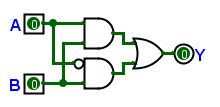
\includegraphics[width=\maxwidth{.95\linewidth}]{gfx/06_01}
	\caption{Simple Circuit For K-Map}
	\label{fig:06_01}
\end{figure}

\begin{align}
  \label{KM:eq:simple_circuit_for_karnaugh_map}
  AB+A'B &= Y
\end{align}

\begin{table}[H]
  \sffamily
  \newcommand{\head}[1]{\textcolor{white}{\textbf{#1}}}    
  \begin{center}
    \rowcolors{2}{gray!10}{white} % Color every other line a light gray
    \begin{tabular}{ccc} 
      \rowcolor{black!75}
      \multicolumn{2}{c}{\head{Inputs}} & \head{Output} \\
      A & B & Y \\
      \hline
      0 & 0 & 0 \\
      0 & 1 & 1 \\
      1 & 0 & 0 \\
      1 & 1 & 1 
    \end{tabular}
  \end{center}
  \caption{Truth Table for Simple Circuit}
  \label{KM:tab:truth_table_simple_circuit}
\end{table}

%****************************************************************
% Karnaugh map For Simple Circuit
%****************************************************************
\begin{figure}[H]
  \caption{Karnaugh map for Simple Circuit}
  \label{KM:tab:k-map_for_simple_circuit}
  \myfloatalign
  \begin{tikzpicture} [circuit logic US, scale=1.00]
  % make all path lines (the node shapes) a little thicker
  \tikzstyle{every path}=[line width=0.50mm]
  
  %********************************************************************
  % Adjust the settings below to display the 1's and rectangles
  %********************************************************************
  % Uncomment the appropriate lines below to insert ones where needed
    \node[] at (1.4,1.5) {\huge $ 0 $}; % 00
    \node[] at (1.4,0.5) {\huge $ 1 $}; % 01
    \node[] at (2.4,1.5) {\huge $ 0 $}; % 02
    \node[] at (2.4,0.5) {\huge $ 1 $}; % 03
  
  % The coords for each cell - this is used as the origin for the solution box
  \coordinate (cell00) at (1.0,3.0); \coordinate (cell01) at (1.0,2.0);
  \coordinate (cell02) at (1.0,0.0); \coordinate (cell03) at (1.0,1.0);
      
  %********************************************************************
  % Shouldn't need to adjust anything below this point - this is just
  % the grid and the minterms.
  %********************************************************************  
  % Text in top-Left cell
  \node[] at (0.35,2.22) { \footnotesize $ \mathsf{ B } $ }; % B
  \node[] at (0.70,2.75) { \footnotesize $ \mathsf{ A } $ }; % A
  
  % Populate the top row header
  % In the following, the foreach lists a location/text pair
  % The the draw line draws the text at each location
  \foreach \loc/\txt in {
    (1.5,2.5)/{0},(2.5,2.5)/{1}
  }
  \draw \loc node{\large $\txt$};
  
  % Populate the header in column one
  \foreach \loc/\txt in { 
    (0.5,1.5)/{0},(0.5,0.5)/{1}
  }
  \draw \loc node{\large $\txt$};
  
  % Populate the minterms
  \foreach \loc/\txt in { 
    (1.75,1.15)/{00} , (2.75,1.15)/{02} , (1.75,0.15)/{01} , (2.75,0.15)/{03} 
    }
  \draw \loc node{ \color{blue!90!black} \footnotesize { $\txt$ }};
  
  % Draw the lines
  \draw
  % Finish drawing the grid
  [step=1.0cm,black,thin] (0,0) grid (3.0,3.0) % The Grid
  (0.0,3.0) -- (1.0,2.0) % Diagonal in the top left cell
  (1.0,2.05) -- (3.0,2.05) % Double line under top header row
  (0.95,0.0) -- (0.95,2.0) % Double line on left of header column one
  ;    
  \end{tikzpicture}
\end{figure}

% Pull Quote - Marginal Note - Sidebar
\marginpar{Karnaugh maps frequently include the minterm numbers in each cell to aid in placing variables.}

First is a circuit diagram, followed by its Boolean equation, truth table, and, finally, Karnaugh map. Think of a Karnaugh map as simply a rearranged truth table; but simplifying a three or four input circuit using a Karnaugh map is much easier and more accurate than with either a truth table or Boolean equation. 

\section{Drawing Two-Variable Karnaugh maps}
\label{KM:sec:drawing_2_variable_karnaugh_maps}

Truth Table \ref{KM:tab:truth_table_with_greek_letters} and Karnaugh map \ref{KM:fig:k-map_with_greek_letters} illustrate the relationship between these two representations of the same circuit using Greek symbols. 

% Table
\begin{table}[H]
  \sffamily
  \newcommand{\head}[1]{\textcolor{white}{\textbf{#1}}}    
  \begin{center}
    \rowcolors{2}{gray!10}{white} % Color every other line a light gray
    \begin{tabular}{ccc} 
      \rowcolor{black!75}
      \multicolumn{2}{c}{\head{Inputs}} & \head{Output} \\
      A & B & Y \\
      \hline
      0 & 0 & $ \alpha $ \\
      0 & 1 & $ \beta $ \\
      1 & 0 & $ \gamma $ \\
      1 & 1 & $ \delta $ 
    \end{tabular}
  \end{center}
  \caption{Truth Table with Greek Letters}
  \label{KM:tab:truth_table_with_greek_letters}
\end{table}

%****************************************************************
% Karnaugh map For 2-Input Circuit With Greek Letters
%****************************************************************
\begin{figure}[H]
  \caption{Karnaugh map With Greek Letters}
  \label{KM:fig:k-map_with_greek_letters}
  \myfloatalign
  \begin{tikzpicture} [circuit logic US, scale=1.00]
  % make all path lines (the node shapes) a little thicker
  \tikzstyle{every path}=[line width=0.50mm]
  
  %********************************************************************
  % Adjust the settings below to display the 1's and rectangles
  %********************************************************************
  % Uncomment the appropriate lines below to insert ones where needed
  \node[] at (1.4,1.5) {\huge $ \alpha $}; % 00
  \node[] at (1.4,0.5) {\huge $ \beta $}; % 01
  \node[] at (2.4,1.5) {\huge $ \gamma $}; % 02
  \node[] at (2.4,0.5) {\huge $ \delta $}; % 03
  
  % The coords for each cell - this is used as the origin for the solution box
  \coordinate (cell00) at (1.0,1.0); \coordinate (cell01) at (1.0,0.0);
  \coordinate (cell02) at (2.0,1.0); \coordinate (cell03) at (2.0,0.0);
  
  %********************************************************************
  % Shouldn't need to adjust anything below this point - this is just
  % the grid and the minterms.
  %********************************************************************  
  % Text in top-Left cell
  \node[] at (0.35,2.22) { \footnotesize $ \mathsf{ B } $ }; % B
  \node[] at (0.70,2.75) { \footnotesize $ \mathsf{ A } $ }; % A
  
  % Populate the top row header
  % In the following, the foreach lists a location/text pair
  % The the draw line draws the text at each location
  \foreach \loc/\txt in {
    (1.5,2.5)/{0},(2.5,2.5)/{1}
  }
  \draw \loc node{\large $\txt$};
  
  % Populate the header in column one
  \foreach \loc/\txt in { 
    (0.5,1.5)/{0},(0.5,0.5)/{1}
  }
  \draw \loc node{\large $\txt$};
  
  % Populate the minterms
  \foreach \loc/\txt in { 
    (1.75,1.15)/{00} , (2.75,1.15)/{02} , (1.75,0.15)/{01} , (2.75,0.15)/{03} 
  }
  \draw \loc node{ \color{blue!90!black} \footnotesize { $\txt$ }};
  
  % Draw the lines
  \draw
  % Finish drawing the grid
  [step=1.0cm,black,thin] (0,0) grid (3.0,3.0) % The Grid
  (0.0,3.0) -- (1.0,2.0) % Diagonal in the top left cell
  (1.0,2.05) -- (3.0,2.05) % Double line under top header row
  (0.95,0.0) -- (0.95,2.0) % Double line on left of header column one
  ;    
  \end{tikzpicture}
\end{figure}

On the Karnaugh map, all of the possible values for input $ A $ are listed across the top of the map and values for input $ B $ are listed down the left side. Thus, to find the output for $ A=0 $; $ B=0 $, look for the cell where those two quantities intersect; which is output $ \alpha $ in the example. It should be clear how all four data squares on the Karnaugh map correspond to their equivalent rows (the minterms) in the Truth Table. 

Truth Table \ref{KM:tab:truth_table_for_2-input_circuit} and Karnaugh map \ref{KM:fig:k-map_for_2_input_circuit} illustrate another example of this relationship.

% Truth Table
\begin{table}[H]
  \sffamily
  \newcommand{\head}[1]{\textcolor{white}{\textbf{#1}}}    
  \begin{center}
    \rowcolors{2}{gray!10}{white} % Color every other line a light gray
    \begin{tabular}{ccc} 
      \rowcolor{black!75}
      \multicolumn{2}{c}{\head{Inputs}} & \head{Output} \\
      A & B & Y \\
      \hline
      0 & 0 & 1 \\
      0 & 1 & 1 \\
      1 & 0 & 0 \\
      1 & 1 & 1 
    \end{tabular}
  \end{center}
  \caption{Truth Table for Two-Input Circuit}
  \label{KM:tab:truth_table_for_2-input_circuit}
\end{table}

%****************************************************************
% Karnaugh map For 2-Input Circuit 
%****************************************************************
\begin{figure}[H]
  \caption{Karnaugh map For Two-Input Circuit}
  \label{KM:fig:k-map_for_2_input_circuit}
  \myfloatalign
  \begin{tikzpicture} [circuit logic US, scale=1.00]
  % make all path lines (the node shapes) a little thicker
  \tikzstyle{every path}=[line width=0.50mm]
  
  %********************************************************************
  % Adjust the settings below to display the 1's and rectangles
  %********************************************************************
  % Uncomment the appropriate lines below to insert ones where needed
  \node[] at (1.4,1.5) {\huge $ 1 $}; % 00
  \node[] at (1.4,0.5) {\huge $ 1 $}; % 01
%  \node[] at (2.4,1.5) {\huge $ 1 $}; % 02
  \node[] at (2.4,0.5) {\huge $ 1 $}; % 03
  
  % The coords for each cell - this is used as the origin for the solution box
  \coordinate (cell00) at (1.0,1.0); \coordinate (cell01) at (1.0,0.0);
  \coordinate (cell02) at (2.0,1.0); \coordinate (cell03) at (2.0,0.0);
  
  %********************************************************************
  % Shouldn't need to adjust anything below this point - this is just
  % the grid and the minterms.
  %********************************************************************  
  % Text in top-Left cell
  \node[] at (0.35,2.22) { \footnotesize $ \mathsf{ B } $ }; % B
  \node[] at (0.70,2.75) { \footnotesize $ \mathsf{ A } $ }; % A
  
  % Populate the top row header
  % In the following, the foreach lists a location/text pair
  % The the draw line draws the text at each location
  \foreach \loc/\txt in {
    (1.5,2.5)/{0},(2.5,2.5)/{1}
  }
  \draw \loc node{\large $\txt$};
  
  % Populate the header in column one
  \foreach \loc/\txt in { 
    (0.5,1.5)/{0},(0.5,0.5)/{1}
  }
  \draw \loc node{\large $\txt$};
  
  % Populate the minterms
  \foreach \loc/\txt in { 
    (1.75,1.15)/{00} , (2.75,1.15)/{02} , (1.75,0.15)/{01} , (2.75,0.15)/{03} 
  }
  \draw \loc node{ \color{blue!90!black} \footnotesize { $\txt$ }};
  
  % Draw the lines
  \draw
  % Finish drawing the grid
  [step=1.0cm,black,thin] (0,0) grid (3.0,3.0) % The Grid
  (0.0,3.0) -- (1.0,2.0) % Diagonal in the top left cell
  (1.0,2.05) -- (3.0,2.05) % Double line under top header row
  (0.95,0.0) -- (0.95,2.0) % Double line on left of header column one
  ;    
  \end{tikzpicture}
\end{figure}
\marginpar{Karnaugh maps usually do not include zeros to decrease the chance for error.}

\section{Drawing Three-Variable Karnaugh maps}
\label{KM:sec:drawing_3-variable_karnaugh_maps}

Consider Equation \ref{KM:eq:karnaugh_map_for_3_variables}.

\begin{align}
  \label{KM:eq:karnaugh_map_for_3_variables}
  ABC'+AB'C+A'B'C &= Y
\end{align}

Table \ref{KM:tab:truth_table_for_3-input_circuit} and Karnaugh map \ref{KM:fig:k-map_for_3-input_circuit} represent this equation.

% Truth Table
\begin{table}[H]
  \sffamily
  \newcommand{\head}[1]{\textcolor{white}{\textbf{#1}}}    
  \begin{center}
    \rowcolors{2}{gray!10}{white} % Color every other line a light gray
    \begin{tabular}{ccccc} 
      \rowcolor{black!75}
      \multicolumn{3}{c}{\head{Inputs}} & \multicolumn{2}{l}{\head{Output}} \\
      A & B & C & Y & minterm \\
      \hline
      0 & 0 & 0 & 0 & 0 \\
      0 & 0 & 1 & 1 & 1 \\
      0 & 1 & 0 & 0 & 2 \\
      0 & 1 & 1 & 0 & 3 \\ 
      1 & 0 & 0 & 0 & 4 \\
      1 & 0 & 1 & 1 & 5 \\
      1 & 1 & 0 & 1 & 6 \\
      1 & 1 & 1 & 0 & 7  
    \end{tabular}
  \end{center}
  \caption{Truth Table for Three-Input Circuit}
  \label{KM:tab:truth_table_for_3-input_circuit}
\end{table}

%****************************************************************
% Karnaugh map For 3-Input Circuit
%****************************************************************
\begin{figure}[H]
  \caption{Karnaugh map for Three-Input Circuit}
  \label{KM:fig:k-map_for_3-input_circuit}
  \myfloatalign
  \begin{tikzpicture} [circuit logic US, scale=1.00]
  % make all path lines (the node shapes) a little thicker
  \tikzstyle{every path}=[line width=0.50mm]
  
  %********************************************************************
  % Adjust the settings below to display the 1's and rectangles
  %********************************************************************
  % Uncomment the appropriate lines below to insert ones where needed
  %  \node[] at (1.4,1.5) {\huge $ 1 $}; % 00
    \node[] at (1.4,0.5) {\huge $ 1 $}; % 01
  %  \node[] at (2.4,1.5) {\huge $ 1 $}; % 02
  %  \node[] at (2.4,0.5) {\huge $ 1 $}; % 03
  %  \node[] at (4.4,1.5) {\huge $ 1 $}; % 04
    \node[] at (4.4,0.5) {\huge $ 1 $}; % 05
    \node[] at (3.4,1.5) {\huge $ 1 $}; % 06
  %  \node[] at (3.4,0.5) {\huge $ 1 $}; % 07
  
  % The coords for each cell - this is used as the origin for the solution box
  \coordinate (cell00) at (1.0,1.0); \coordinate (cell01) at (1.0,0.0);
  \coordinate (cell02) at (2.0,1.0); \coordinate (cell03) at (2.0,0.0);
  
  \coordinate (cell04) at (4.0,1.0); \coordinate (cell05) at (4.0,0.0);
  \coordinate (cell06) at (3.0,1.0); \coordinate (cell07) at (3.0,0.0);
    
  %********************************************************************
  % Shouldn't need to adjust anything below this point - this is just
  % the grid and the minterms.
  %********************************************************************  
  % Text in top-Left cell
  \node[] at (0.35,2.22) { \footnotesize $ \mathsf{ C } $ }; % C
  \node[] at (0.70,2.75) { \footnotesize $ \mathsf{ AB } $ }; % ab
  
  % Populate the top row header
  % In the following, the foreach lists a location/text pair
  % The the draw line draws the text at each location
  \foreach \loc/\txt in {
    (1.5,2.5)/{00},(2.5,2.5)/{01},(3.5,2.5)/{11},(4.5,2.5)/{10}
  }
  \draw \loc node{\large $\txt$};
  
  % Populate the header in column one
  \foreach \loc/\txt in { 
    (0.5,1.5)/{0},(0.5,0.5)/{1}
  }
  \draw \loc node{\large $\txt$};
  
  % Populate the minterms
  \foreach \loc/\txt in { 
    (1.75,1.15)/{00} , (2.75,1.15)/{02} , (3.75,1.15)/{06} , (4.75,1.15)/{04} ,
    (1.75,0.15)/{01} , (2.75,0.15)/{03} , (3.75,0.15)/{07} , (4.75,0.15)/{05} }
  \draw \loc node{ \color{blue!90!black} \footnotesize { $\txt$ }};
  
  % Draw the lines
  \draw
  % Finish drawing the grid
  [step=1.0cm,black,thin] (0,0) grid (5.0,3.0) % The Grid
  (0.0,3.0) -- (1.0,2.0) % Diagonal in the top left cell
  (1.0,2.05) -- (5.0,2.05) % Double line under top header row
  (0.95,0.0) -- (0.95,2.0) % Double line on left of header column one
  ;    
  \end{tikzpicture}
\end{figure}

In Karnaugh map \ref{KM:fig:k-map_for_3-input_circuit} all possible values for inputs $ A $ and $ B $ are listed across the top of the map while input $ C $ is listed down the left side. Therefore, minterm $ m_{05} $, in the lower right corner of the Karnaugh map, is for $ A=1 $; $ B=0 $; $ C=1 $, ($ AB'C $), one of the \emph{True} terms in the original equation. 

\subsection{The Gray Code}
\label{KM:subsec:the_gray_code_for_karnaugh_maps}

It should be noted that the values across the top of the Karnaugh map are not in binary order. Instead, those values are in ``Gray Code'' order. Gray code is essential for a Karnaugh map since the values for adjacent cells must change by only one bit. Constructing the Gray Code for three, four, and five variables is covered on page \pageref{MO:subsub:gray_code}; however, for the Karnaugh maps used in this chapter, it is enough to know the two-bit Gray code: $ 00 $, $ 01 $, $ 11 $, $ 10 $. 

\section{Drawing Four-Variable Karnaugh maps}
\label{KM:sec:drawing_4-variable_karnaugh_maps}

Consider Equation \ref{KM:eq:karnaugh_map_for_4_variables}.

\begin{align}
  \label{KM:eq:karnaugh_map_for_4_variables}
  ABCD'+AB'CD+A'B'CD &= Y
\end{align}

Table \ref{KM:tab:truth_table_for_4-input_circuit} and the Karnaugh map in Figure \ref{KM:fig:kmap_for_four_input_circuit} illustrate this equation.

% Truth Table
\begin{table}[H]
  \sffamily
  \newcommand{\head}[1]{\textcolor{white}{\textbf{#1}}}    
  \begin{center}
    \rowcolors{2}{gray!10}{white} % Color every other line a light gray
    \begin{tabular}{cccccc} 
      \rowcolor{black!75}
      \multicolumn{4}{c}{\head{Inputs}} & \multicolumn{2}{l}{\head{Output}} \\
      A & B & C & D & Y & minterm \\
      \hline
      0 & 0 & 0 & 0 & 0 & 0 \\
      0 & 0 & 0 & 1 & 0 & 1 \\
      0 & 0 & 1 & 0 & 0 & 2 \\
      0 & 0 & 1 & 1 & 1 & 3 \\ 
      0 & 1 & 0 & 0 & 0 & 4 \\
      0 & 1 & 0 & 1 & 0 & 5 \\
      0 & 1 & 1 & 0 & 0 & 6 \\
      1 & 1 & 1 & 1 & 0 & 7 \\
      1 & 0 & 0 & 0 & 0 & 8 \\
      1 & 0 & 0 & 1 & 0 & 9 \\
      1 & 0 & 1 & 0 & 0 & 10 \\
      1 & 0 & 1 & 1 & 1 & 11 \\ 
      1 & 1 & 0 & 0 & 0 & 12 \\
      1 & 1 & 0 & 1 & 0 & 13 \\
      1 & 1 & 1 & 0 & 1 & 14 \\
      1 & 1 & 1 & 1 & 0 & 15  
    \end{tabular}
  \end{center}
  \caption{Truth Table for Four-Input Circuit}
  \label{KM:tab:truth_table_for_4-input_circuit}
\end{table}

%****************************************************************
% Karnaugh map for 4-Input Circuit
%****************************************************************
\begin{figure}[H]
  \caption{K-Map For Four Input Circuit}
  \label{KM:fig:kmap_for_four_input_circuit}
  \myfloatalign
  \begin{tikzpicture} [circuit logic US, scale=1.00]
  % make all path lines (the node shapes) a little thicker
  \tikzstyle{every path}=[line width=0.50mm]
  
  %********************************************************************
  % Adjust the settings below to display the 1's and rectangles
  %********************************************************************
  % Uncomment the appropriate lines below to insert ones where needed
%  \node[] at (1.4,3.5) {\huge $ 1 $}; % 00
%  \node[] at (1.4,2.5) {\huge $ 1 $}; % 01
%  \node[] at (1.4,0.5) {\huge $ 1 $}; % 02
  \node[] at (1.4,1.5) {\huge $ 1 $}; % 03
%  \node[] at (2.4,3.5) {\huge $ 1 $}; % 04
%  \node[] at (2.4,2.5) {\huge $ 1 $}; % 05
%  \node[] at (2.4,0.5) {\huge $ 1 $}; % 06
%  \node[] at (2.4,1.5) {\huge $ 1 $}; % 07
%  \node[] at (4.4,3.5) {\huge $ 1 $}; % 08
%  \node[] at (4.4,2.5) {\huge $ 1 $}; % 09
%  \node[] at (4.4,0.5) {\huge $ 1 $}; % 10
  \node[] at (4.4,1.5) {\huge $ 1 $}; % 11
%  \node[] at (3.4,3.5) {\huge $ 1 $}; % 12
%  \node[] at (3.4,2.5) {\huge $ 1 $}; % 13
  \node[] at (3.4,0.5) {\huge $ 1 $}; % 14
%  \node[] at (3.4,1.5) {\huge $ 1 $}; % 15
  
  % The coords for each cell - this is used as the origin for the solution box
  \coordinate (cell00) at (1.0,3.0); \coordinate (cell01) at (1.0,2.0);
  \coordinate (cell02) at (1.0,0.0); \coordinate (cell03) at (1.0,1.0);

  \coordinate (cell04) at (2.0,3.0); \coordinate (cell05) at (2.0,2.0);
  \coordinate (cell06) at (2.0,0.0); \coordinate (cell07) at (2.0,1.0);

  \coordinate (cell12) at (3.0,3.0); \coordinate (cell13) at (3.0,2.0);
  \coordinate (cell14) at (3.0,0.0); \coordinate (cell15) at (3.0,1.0);

  \coordinate (cell08) at (4.0,3.0); \coordinate (cell09) at (4.0,2.0);
  \coordinate (cell10) at (4.0,0.0); \coordinate (cell11) at (4.0,1.0);
  
  % Horizontal Group
%  \node [draw,
%  color=red!70!black,
%  fill=red!20!white,
%  fill opacity=0.3,
%  minimum height=0.95cm,
%  minimum width=1.95cm, % Adjust to (number of cells) * 1 - 0.95
%  rounded corners,
%  anchor=south west] at (cell02) {}; % Enter left cell minterm
  
  % Vertical Group
%  \node [draw,
%  color=blue!70!black,
%  fill=blue!20!white,
%  fill opacity=0.3,
%  minimum height=1.95cm, % Adjust to (number of cells) * 1 - 0.95
%  minimum width=0.95cm,
%  rounded corners,
%  anchor=south west] at (cell07) {}; % Enter bottom cell minterm
  
  % Single Cell
%  \node [draw,
%  color=green!70!black,
%  fill=green!20!white,
%  fill opacity=0.3,
%  minimum height=0.95cm,
%  minimum width=0.95cm,
%  rounded corners,
%  anchor=south west] at (cell09) {}; % Enter cell minterm
  
  %********************************************************************
  % Shouldn't need to adjust anything below this point - this is just
  % the grid and the minterms.
  %********************************************************************  
  % Text in top-Left cell
  \node[] at (0.35,4.22) { \footnotesize $ \mathsf{ CD } $ }; % cd
  \node[] at (0.70,4.75) { \footnotesize $ \mathsf{ AB } $ }; % ab
  
  % Populate the top row header
  % In the following, the foreach lists a location/text pair
  % The the draw line draws the text at each location
  \foreach \loc/\txt in {
    (1.5,4.5)/{00},(2.5,4.5)/{01},(3.5,4.5)/{11},(4.5,4.5)/{10}
  }
  \draw \loc node{\large $\txt$};
  
  % Populate the header in column one
  \foreach \loc/\txt in { 
    (0.5,3.5)/{00},(0.5,2.5)/{01},(0.5,1.5)/{11},(0.5,0.5)/{10}
  }
  \draw \loc node{\large $\txt$};
  
  % Populate the minterms
  \foreach \loc/\txt in { 
    (1.75,3.15)/{00} , (2.75,3.15)/{04} , (3.75,3.15)/{12} , (4.75,3.15)/{08} ,
    (1.75,2.15)/{01} , (2.75,2.15)/{05} , (3.75,2.15)/{13} , (4.75,2.15)/{09} ,
    (1.75,1.15)/{03} , (2.75,1.15)/{07} , (3.75,1.15)/{15} , (4.75,1.15)/{11} ,
    (1.75,0.15)/{02} , (2.75,0.15)/{06} , (3.75,0.15)/{14} , (4.75,0.15)/{10} }
  \draw \loc node{ \color{blue!90!black} \footnotesize { $\txt$ }};
  
  % Draw the lines
  \draw
  % Finish drawing the grid
  [step=1.0cm,black,thin] (0,0) grid (5.0,5.0) % The Grid
  (0.0,5.0) -- (1.0,4.0) % Diagonal in the top left cell
  (1.0,4.05) -- (5.0,4.05) % Double line under top header row
  (0.95,0.0) -- (0.95,4.0) % Double line on left of header column one
  ;    
  \end{tikzpicture}
\end{figure}

This Karnaugh map is similar to those for two and three variables, but the top row is for the $ A $ and $ B $ inputs while the left column is for the $ C $ and $ D $ inputs. Notice that the values in both the top row and left column use Gray Code sequencing rather than binary counting.

It is easy to indicate the minterms that are \emph{True} on a Karnaugh map if Sigma Notation is available since the numbers following the Sigma sign are the minterms. As an example, Equation \ref{KM:eq:karnaugh_map_when_given_the_sigma_function} creates the Karnaugh map in Figure \ref{KM:fig:kmap_for_sigma_notation}. 

\begin{align}
  \label{KM:eq:karnaugh_map_when_given_the_sigma_function}
  \int{(A,B,C,D)} = \sum(0,1,2,4,5)
\end{align}

%****************************************************************
% Karnaugh map For a Sigma Function
%****************************************************************
\begin{figure}[H]
  \caption{K-Map For Sigma Notation}
  \label{KM:fig:kmap_for_sigma_notation}
  \myfloatalign
  \begin{tikzpicture} [circuit logic US, scale=1.00]
  % make all path lines (the node shapes) a little thicker
  \tikzstyle{every path}=[line width=0.50mm]
  
  %********************************************************************
  % Adjust the settings below to display the 1's and rectangles
  %********************************************************************
  % Uncomment the appropriate lines below to insert ones where needed
    \node[] at (1.4,3.5) {\huge $ 1 $}; % 00
    \node[] at (1.4,2.5) {\huge $ 1 $}; % 01
    \node[] at (1.4,0.5) {\huge $ 1 $}; % 02
  %  \node[] at (1.4,1.5) {\huge $ 1 $}; % 03
    \node[] at (2.4,3.5) {\huge $ 1 $}; % 04
    \node[] at (2.4,2.5) {\huge $ 1 $}; % 05
  %  \node[] at (2.4,0.5) {\huge $ 1 $}; % 06
  %  \node[] at (2.4,1.5) {\huge $ 1 $}; % 07
  %  \node[] at (4.4,3.5) {\huge $ 1 $}; % 08
  %  \node[] at (4.4,2.5) {\huge $ 1 $}; % 09
  %  \node[] at (4.4,0.5) {\huge $ 1 $}; % 10
  %  \node[] at (4.4,1.5) {\huge $ 1 $}; % 11
  %  \node[] at (3.4,3.5) {\huge $ 1 $}; % 12
  %  \node[] at (3.4,2.5) {\huge $ 1 $}; % 13
  %  \node[] at (3.4,0.5) {\huge $ 1 $}; % 14
  %  \node[] at (3.4,1.5) {\huge $ 1 $}; % 15
  
  % The coords for each cell - this is used as the origin for the solution box
  \coordinate (cell00) at (1.0,3.0); \coordinate (cell01) at (1.0,2.0);
  \coordinate (cell02) at (1.0,0.0); \coordinate (cell03) at (1.0,1.0);
  
  \coordinate (cell04) at (2.0,3.0); \coordinate (cell05) at (2.0,2.0);
  \coordinate (cell06) at (2.0,0.0); \coordinate (cell07) at (2.0,1.0);
  
  \coordinate (cell12) at (3.0,3.0); \coordinate (cell13) at (3.0,2.0);
  \coordinate (cell14) at (3.0,0.0); \coordinate (cell15) at (3.0,1.0);
  
  \coordinate (cell08) at (4.0,3.0); \coordinate (cell09) at (4.0,2.0);
  \coordinate (cell10) at (4.0,0.0); \coordinate (cell11) at (4.0,1.0);
  
  % Horizontal Group
  %  \node [draw,
  %  color=red!70!black,
  %  fill=red!20!white,
  %  fill opacity=0.3,
  %  minimum height=0.95cm,
  %  minimum width=1.95cm, % Adjust to (number of cells) * 1 - 0.95
  %  rounded corners,
  %  anchor=south west] at (cell02) {}; % Enter left cell minterm
  
  % Vertical Group
  %  \node [draw,
  %  color=blue!70!black,
  %  fill=blue!20!white,
  %  fill opacity=0.3,
  %  minimum height=1.95cm, % Adjust to (number of cells) * 1 - 0.95
  %  minimum width=0.95cm,
  %  rounded corners,
  %  anchor=south west] at (cell07) {}; % Enter bottom cell minterm
  
  % Single Cell
  %  \node [draw,
  %  color=green!70!black,
  %  fill=green!20!white,
  %  fill opacity=0.3,
  %  minimum height=0.95cm,
  %  minimum width=0.95cm,
  %  rounded corners,
  %  anchor=south west] at (cell09) {}; % Enter cell minterm
  
  %********************************************************************
  % Shouldn't need to adjust anything below this point - this is just
  % the grid and the minterms.
  %********************************************************************  
  % Text in top-Left cell
  \node[] at (0.35,4.22) { \footnotesize $ \mathsf{ CD } $ }; % cd
  \node[] at (0.70,4.75) { \footnotesize $ \mathsf{ AB } $ }; % ab
  
  % Populate the top row header
  % In the following, the foreach lists a location/text pair
  % The the draw line draws the text at each location
  \foreach \loc/\txt in {
    (1.5,4.5)/{00},(2.5,4.5)/{01},(3.5,4.5)/{11},(4.5,4.5)/{10}
  }
  \draw \loc node{\large $\txt$};
  
  % Populate the header in column one
  \foreach \loc/\txt in { 
    (0.5,3.5)/{00},(0.5,2.5)/{01},(0.5,1.5)/{11},(0.5,0.5)/{10}
  }
  \draw \loc node{\large $\txt$};
  
  % Populate the minterms
  \foreach \loc/\txt in { 
    (1.75,3.15)/{00} , (2.75,3.15)/{04} , (3.75,3.15)/{12} , (4.75,3.15)/{08} ,
    (1.75,2.15)/{01} , (2.75,2.15)/{05} , (3.75,2.15)/{13} , (4.75,2.15)/{09} ,
    (1.75,1.15)/{03} , (2.75,1.15)/{07} , (3.75,1.15)/{15} , (4.75,1.15)/{11} ,
    (1.75,0.15)/{02} , (2.75,0.15)/{06} , (3.75,0.15)/{14} , (4.75,0.15)/{10} }
  \draw \loc node{ \color{blue!90!black} \footnotesize { $\txt$ }};
  
  % Draw the lines
  \draw
  % Finish drawing the grid
  [step=1.0cm,black,thin] (0,0) grid (5.0,5.0) % The Grid
  (0.0,5.0) -- (1.0,4.0) % Diagonal in the top left cell
  (1.0,4.05) -- (5.0,4.05) % Double line under top header row
  (0.95,0.0) -- (0.95,4.0) % Double line on left of header column one
  ;    
  \end{tikzpicture}
\end{figure}

It is also possible to map values if the circuit is represented in Pi notation; but remember that maxterms indicate where zeros are placed on the Karnaugh map and the simplified circuit would actually be the inverse of the needed circuit. As an example, Equation \ref{KM:eq:karnaugh_map_when_given_the_pi_function} creates the Karnaugh map at Figure \ref{KM:fig:kmap_for_pi_notation}. 

\begin{align}
  \label{KM:eq:karnaugh_map_when_given_the_pi_function}
  \int{(A,B,C,D)} = \prod(8,9,12,13)
\end{align}

%****************************************************************
% Karnaugh map for a PI Function
%****************************************************************
\begin{figure}[H]
  \caption{K-Map For PI Notation}
  \label{KM:fig:kmap_for_pi_notation}
  \myfloatalign
  \begin{tikzpicture} [circuit logic US, scale=1.00]
  % make all path lines (the node shapes) a little thicker
  \tikzstyle{every path}=[line width=0.50mm]
  
  %********************************************************************
  % Adjust the settings below to display the 1's and rectangles
  %********************************************************************
  % Uncomment the appropriate lines below to insert ones where needed
  %  \node[] at (1.4,3.5) {\huge $ 0 $}; % 00
  %  \node[] at (1.4,2.5) {\huge $ 0 $}; % 01
  %  \node[] at (1.4,0.5) {\huge $ 0 $}; % 02
  %  \node[] at (1.4,1.5) {\huge $ 0 $}; % 03
  %  \node[] at (2.4,3.5) {\huge $ 0 $}; % 04
  %  \node[] at (2.4,2.5) {\huge $ 0 $}; % 05
  %  \node[] at (2.4,0.5) {\huge $ 0 $}; % 06
  %  \node[] at (2.4,1.5) {\huge $ 0 $}; % 07
    \node[] at (4.4,3.5) {\huge $ 0 $}; % 08
    \node[] at (4.4,2.5) {\huge $ 0 $}; % 09
  %  \node[] at (4.4,0.5) {\huge $ 0 $}; % 10
  %  \node[] at (4.4,1.5) {\huge $ 0 $}; % 11
    \node[] at (3.4,3.5) {\huge $ 0 $}; % 12
    \node[] at (3.4,2.5) {\huge $ 0 $}; % 13
  %  \node[] at (3.4,0.5) {\huge $ 0 $}; % 14
  %  \node[] at (3.4,1.5) {\huge $ 0 $}; % 15
  
  % The coords for each cell - this is used as the origin for the solution box
  \coordinate (cell00) at (1.0,3.0); \coordinate (cell01) at (1.0,2.0);
  \coordinate (cell02) at (1.0,0.0); \coordinate (cell03) at (1.0,1.0);
  
  \coordinate (cell04) at (2.0,3.0); \coordinate (cell05) at (2.0,2.0);
  \coordinate (cell06) at (2.0,0.0); \coordinate (cell07) at (2.0,1.0);
  
  \coordinate (cell12) at (3.0,3.0); \coordinate (cell13) at (3.0,2.0);
  \coordinate (cell14) at (3.0,0.0); \coordinate (cell15) at (3.0,1.0);
  
  \coordinate (cell08) at (4.0,3.0); \coordinate (cell09) at (4.0,2.0);
  \coordinate (cell10) at (4.0,0.0); \coordinate (cell11) at (4.0,1.0);
  
  % Horizontal Group
  %  \node [draw,
  %  color=red!70!black,
  %  fill=red!20!white,
  %  fill opacity=0.3,
  %  minimum height=0.95cm,
  %  minimum width=1.95cm, % Adjust to (number of cells) * 1 - 0.95
  %  rounded corners,
  %  anchor=south west] at (cell02) {}; % Enter left cell minterm
  
  % Vertical Group
  %  \node [draw,
  %  color=blue!70!black,
  %  fill=blue!20!white,
  %  fill opacity=0.3,
  %  minimum height=1.95cm, % Adjust to (number of cells) * 1 - 0.95
  %  minimum width=0.95cm,
  %  rounded corners,
  %  anchor=south west] at (cell07) {}; % Enter bottom cell minterm
  
  % Single Cell
  %  \node [draw,
  %  color=green!70!black,
  %  fill=green!20!white,
  %  fill opacity=0.3,
  %  minimum height=0.95cm,
  %  minimum width=0.95cm,
  %  rounded corners,
  %  anchor=south west] at (cell09) {}; % Enter cell minterm
  
  %********************************************************************
  % Shouldn't need to adjust anything below this point - this is just
  % the grid and the minterms.
  %********************************************************************  
  % Text in top-Left cell
  \node[] at (0.35,4.22) { \footnotesize $ \mathsf{ CD } $ }; % cd
  \node[] at (0.70,4.75) { \footnotesize $ \mathsf{ AB } $ }; % ab
  
  % Populate the top row header
  % In the following, the foreach lists a location/text pair
  % The the draw line draws the text at each location
  \foreach \loc/\txt in {
    (1.5,4.5)/{00},(2.5,4.5)/{01},(3.5,4.5)/{11},(4.5,4.5)/{10}
  }
  \draw \loc node{\large $\txt$};
  
  % Populate the header in column one
  \foreach \loc/\txt in { 
    (0.5,3.5)/{00},(0.5,2.5)/{01},(0.5,1.5)/{11},(0.5,0.5)/{10}
  }
  \draw \loc node{\large $\txt$};
  
  % Populate the minterms
  \foreach \loc/\txt in { 
    (1.75,3.15)/{00} , (2.75,3.15)/{04} , (3.75,3.15)/{12} , (4.75,3.15)/{08} ,
    (1.75,2.15)/{01} , (2.75,2.15)/{05} , (3.75,2.15)/{13} , (4.75,2.15)/{09} ,
    (1.75,1.15)/{03} , (2.75,1.15)/{07} , (3.75,1.15)/{15} , (4.75,1.15)/{11} ,
    (1.75,0.15)/{02} , (2.75,0.15)/{06} , (3.75,0.15)/{14} , (4.75,0.15)/{10} }
  \draw \loc node{ \color{blue!90!black} \footnotesize { $\txt$ }};
  
  % Draw the lines
  \draw
  % Finish drawing the grid
  [step=1.0cm,black,thin] (0,0) grid (5.0,5.0) % The Grid
  (0.0,5.0) -- (1.0,4.0) % Diagonal in the top left cell
  (1.0,4.05) -- (5.0,4.05) % Double line under top header row
  (0.95,0.0) -- (0.95,4.0) % Double line on left of header column one
  ;    
  \end{tikzpicture}
\end{figure}

To simplify this map, the designer could place ones in all of the empty cells and then simplify the ``ones'' circuit using the techniques explained below. Alternatively, the designer could also simplify the map by combining the zeros as if they were ones, and then finding the DeMorgan inverse (page  \pageref{BF:sec:demorgans_theorem}) of that simplification. As an example, the maxterm Karnaugh map above would simplify to $ \overline{AC'} $, and the DeMorgan equivalent for that is $ A'+C $, which is the minterm version of the simplified circuit.

\section{Simplifying Groups of Two}
\label{KM:sec:simplifying_groups_of_two}

To simplify a Boolean equation using a Karnaugh map, start by creating the Karnaugh map, indicating the input variable combinations that lead to a \emph{True} output for the circuit. Equations \ref{KM:eq:simplifying_4-input_equations_groups_of_two} and \ref{KM:eq:sigma_notation_solving_k-map_groups_of_two} are for the same circuit and the Karnaugh map in Figure \ref{KM:fig:k-map_for_groups_of_two_ex_1} was built from these equations. 

\begin{align}
  \label{KM:eq:simplifying_4-input_equations_groups_of_two}
  A'B'C'D'+A'BC'D'+A'BCD+AB'CD'+AB'CD
\end{align}

\begin{align}
  \label{KM:eq:sigma_notation_solving_k-map_groups_of_two}
  \int{(A,B,C,D)} = \sum(0,4,7,10,11)
\end{align}

%****************************************************************
% Karnaugh map For Groups of 2, Example 1
%****************************************************************
\begin{figure}[H]
  \caption{K-Map for Groups of Two: Ex 1}
  \label{KM:fig:k-map_for_groups_of_two_ex_1}
  \myfloatalign
  \begin{tikzpicture} [circuit logic US, scale=1.00]
  % make all path lines (the node shapes) a little thicker
  \tikzstyle{every path}=[line width=0.50mm]
  
  %********************************************************************
  % Adjust the settings below to display the 1's and rectangles
  %********************************************************************
  % Uncomment the appropriate lines below to insert ones where needed
    \node[] at (1.4,3.5) {\huge $ 1 $}; % 00
  %  \node[] at (1.4,2.5) {\huge $ 1 $}; % 01
  %  \node[] at (1.4,0.5) {\huge $ 1 $}; % 02
  %  \node[] at (1.4,1.5) {\huge $ 1 $}; % 03
    \node[] at (2.4,3.5) {\huge $ 1 $}; % 04
  %  \node[] at (2.4,2.5) {\huge $ 1 $}; % 05
  %  \node[] at (2.4,0.5) {\huge $ 1 $}; % 06
    \node[] at (2.4,1.5) {\huge $ 1 $}; % 07
  %  \node[] at (4.4,3.5) {\huge $ 1 $}; % 08
  %  \node[] at (4.4,2.5) {\huge $ 1 $}; % 09
    \node[] at (4.4,0.5) {\huge $ 1 $}; % 10
    \node[] at (4.4,1.5) {\huge $ 1 $}; % 11
  %  \node[] at (3.4,3.5) {\huge $ 1 $}; % 12
  %  \node[] at (3.4,2.5) {\huge $ 1 $}; % 13
  %  \node[] at (3.4,0.5) {\huge $ 1 $}; % 14
  %  \node[] at (3.4,1.5) {\huge $ 1 $}; % 15
  
  % The coords for each cell - this is used as the origin for the solution box
  \coordinate (cell00) at (1.0,3.0); \coordinate (cell01) at (1.0,2.0);
  \coordinate (cell02) at (1.0,0.0); \coordinate (cell03) at (1.0,1.0);
  
  \coordinate (cell04) at (2.0,3.0); \coordinate (cell05) at (2.0,2.0);
  \coordinate (cell06) at (2.0,0.0); \coordinate (cell07) at (2.0,1.0);
  
  \coordinate (cell12) at (3.0,3.0); \coordinate (cell13) at (3.0,2.0);
  \coordinate (cell14) at (3.0,0.0); \coordinate (cell15) at (3.0,1.0);
  
  \coordinate (cell08) at (4.0,3.0); \coordinate (cell09) at (4.0,2.0);
  \coordinate (cell10) at (4.0,0.0); \coordinate (cell11) at (4.0,1.0);
  
  % Horizontal Group
  %  \node [draw,
  %  color=red!70!black,
  %  fill=red!20!white,
  %  fill opacity=0.3,
  %  minimum height=0.95cm,
  %  minimum width=1.95cm, % Adjust to (number of cells) * 1 - 0.95
  %  rounded corners,
  %  anchor=south west] at (cell02) {}; % Enter left cell minterm
  
  % Vertical Group
  %  \node [draw,
  %  color=blue!70!black,
  %  fill=blue!20!white,
  %  fill opacity=0.3,
  %  minimum height=1.95cm, % Adjust to (number of cells) * 1 - 0.95
  %  minimum width=0.95cm,
  %  rounded corners,
  %  anchor=south west] at (cell07) {}; % Enter bottom cell minterm
  
  % Single Cell
  %  \node [draw,
  %  color=green!70!black,
  %  fill=green!20!white,
  %  fill opacity=0.3,
  %  minimum height=0.95cm,
  %  minimum width=0.95cm,
  %  rounded corners,
  %  anchor=south west] at (cell09) {}; % Enter cell minterm
  
  %********************************************************************
  % Shouldn't need to adjust anything below this point - this is just
  % the grid and the minterms.
  %********************************************************************  
  % Text in top-Left cell
  \node[] at (0.35,4.22) { \footnotesize $ \mathsf{ CD } $ }; % cd
  \node[] at (0.70,4.75) { \footnotesize $ \mathsf{ AB } $ }; % ab
  
  % Populate the top row header
  % In the following, the foreach lists a location/text pair
  % The the draw line draws the text at each location
  \foreach \loc/\txt in {
    (1.5,4.5)/{00},(2.5,4.5)/{01},(3.5,4.5)/{11},(4.5,4.5)/{10}
  }
  \draw \loc node{\large $\txt$};
  
  % Populate the header in column one
  \foreach \loc/\txt in { 
    (0.5,3.5)/{00},(0.5,2.5)/{01},(0.5,1.5)/{11},(0.5,0.5)/{10}
  }
  \draw \loc node{\large $\txt$};
  
  % Populate the minterms
  \foreach \loc/\txt in { 
    (1.75,3.15)/{00} , (2.75,3.15)/{04} , (3.75,3.15)/{12} , (4.75,3.15)/{08} ,
    (1.75,2.15)/{01} , (2.75,2.15)/{05} , (3.75,2.15)/{13} , (4.75,2.15)/{09} ,
    (1.75,1.15)/{03} , (2.75,1.15)/{07} , (3.75,1.15)/{15} , (4.75,1.15)/{11} ,
    (1.75,0.15)/{02} , (2.75,0.15)/{06} , (3.75,0.15)/{14} , (4.75,0.15)/{10} }
  \draw \loc node{ \color{blue!90!black} \footnotesize { $\txt$ }};
  
  % Draw the lines
  \draw
  % Finish drawing the grid
  [step=1.0cm,black,thin] (0,0) grid (5.0,5.0) % The Grid
  (0.0,5.0) -- (1.0,4.0) % Diagonal in the top left cell
  (1.0,4.05) -- (5.0,4.05) % Double line under top header row
  (0.95,0.0) -- (0.95,4.0) % Double line on left of header column one
  ;    
  \end{tikzpicture}
\end{figure}

Once the \emph{True} outputs are indicated on the Karnaugh map, mark any groups of ones that are adjacent to each other, either horizontally or vertically (but not diagonally). Also, mark any ones that are ``left over'' and are not adjacent to any other ones, as illustrated in the Karnaugh map in Figure \ref{KM:fig:kmap_solving_groups_of_two_ex_1}. 

%****************************************************************
% Karnaugh map For Groups of 2, Example 1, Simplified
%****************************************************************
\begin{figure}[H]
  \caption{K-Map for Groups of Two: Ex 1, Solved}
  \label{KM:fig:k-map_for_groups_of_two_ex_1_solved}
  \myfloatalign
  \begin{tikzpicture} [circuit logic US, scale=1.00]
  % make all path lines (the node shapes) a little thicker
  \tikzstyle{every path}=[line width=0.50mm]
  
  %********************************************************************
  % Adjust the settings below to display the 1's and rectangles
  %********************************************************************
  % Uncomment the appropriate lines below to insert ones where needed
  \node[] at (1.4,3.5) {\huge $ 1 $}; % 00
  %  \node[] at (1.4,2.5) {\huge $ 1 $}; % 01
  %  \node[] at (1.4,0.5) {\huge $ 1 $}; % 02
  %  \node[] at (1.4,1.5) {\huge $ 1 $}; % 03
  \node[] at (2.4,3.5) {\huge $ 1 $}; % 04
  %  \node[] at (2.4,2.5) {\huge $ 1 $}; % 05
  %  \node[] at (2.4,0.5) {\huge $ 1 $}; % 06
  \node[] at (2.4,1.5) {\huge $ 1 $}; % 07
  %  \node[] at (4.4,3.5) {\huge $ 1 $}; % 08
  %  \node[] at (4.4,2.5) {\huge $ 1 $}; % 09
  \node[] at (4.4,0.5) {\huge $ 1 $}; % 10
  \node[] at (4.4,1.5) {\huge $ 1 $}; % 11
  %  \node[] at (3.4,3.5) {\huge $ 1 $}; % 12
  %  \node[] at (3.4,2.5) {\huge $ 1 $}; % 13
  %  \node[] at (3.4,0.5) {\huge $ 1 $}; % 14
  %  \node[] at (3.4,1.5) {\huge $ 1 $}; % 15
  
  % The coords for each cell - this is used as the origin for the solution box
  \coordinate (cell00) at (1.0,3.0); \coordinate (cell01) at (1.0,2.0);
  \coordinate (cell02) at (1.0,0.0); \coordinate (cell03) at (1.0,1.0);
  
  \coordinate (cell04) at (2.0,3.0); \coordinate (cell05) at (2.0,2.0);
  \coordinate (cell06) at (2.0,0.0); \coordinate (cell07) at (2.0,1.0);
  
  \coordinate (cell12) at (3.0,3.0); \coordinate (cell13) at (3.0,2.0);
  \coordinate (cell14) at (3.0,0.0); \coordinate (cell15) at (3.0,1.0);
  
  \coordinate (cell08) at (4.0,3.0); \coordinate (cell09) at (4.0,2.0);
  \coordinate (cell10) at (4.0,0.0); \coordinate (cell11) at (4.0,1.0);
  
  % Horizontal Group
    \node [draw,
    color=red!70!black,
    fill=red!20!white,
    fill opacity=0.3,
    minimum height=0.95cm,
    minimum width=1.95cm, % Adjust to (number of cells) * 1 - 0.95
    rounded corners,
    anchor=south west] at (cell00) {}; % Enter left cell minterm
  
  % Vertical Group
    \node [draw,
    color=blue!70!black,
    fill=blue!20!white,
    fill opacity=0.3,
    minimum height=1.95cm, % Adjust to (number of cells) * 1 - 0.95
    minimum width=0.95cm,
    rounded corners,
    anchor=south west] at (cell10) {}; % Enter bottom cell minterm
  
  % Single Cell
    \node [draw,
    color=green!70!black,
    fill=green!20!white,
    fill opacity=0.3,
    minimum height=0.95cm,
    minimum width=0.95cm,
    rounded corners,
    anchor=south west] at (cell07) {}; % Enter cell minterm
  
  %********************************************************************
  % Shouldn't need to adjust anything below this point - this is just
  % the grid and the minterms.
  %********************************************************************  
  % Text in top-Left cell
  \node[] at (0.35,4.22) { \footnotesize $ \mathsf{ CD } $ }; % cd
  \node[] at (0.70,4.75) { \footnotesize $ \mathsf{ AB } $ }; % ab
  
  % Populate the top row header
  % In the following, the foreach lists a location/text pair
  % The the draw line draws the text at each location
  \foreach \loc/\txt in {
    (1.5,4.5)/{00},(2.5,4.5)/{01},(3.5,4.5)/{11},(4.5,4.5)/{10}
  }
  \draw \loc node{\large $\txt$};
  
  % Populate the header in column one
  \foreach \loc/\txt in { 
    (0.5,3.5)/{00},(0.5,2.5)/{01},(0.5,1.5)/{11},(0.5,0.5)/{10}
  }
  \draw \loc node{\large $\txt$};
  
  % Populate the minterms
  \foreach \loc/\txt in { 
    (1.75,3.15)/{00} , (2.75,3.15)/{04} , (3.75,3.15)/{12} , (4.75,3.15)/{08} ,
    (1.75,2.15)/{01} , (2.75,2.15)/{05} , (3.75,2.15)/{13} , (4.75,2.15)/{09} ,
    (1.75,1.15)/{03} , (2.75,1.15)/{07} , (3.75,1.15)/{15} , (4.75,1.15)/{11} ,
    (1.75,0.15)/{02} , (2.75,0.15)/{06} , (3.75,0.15)/{14} , (4.75,0.15)/{10} }
  \draw \loc node{ \color{blue!90!black} \footnotesize { $\txt$ }};
  
  % Draw the lines
  \draw
  % Finish drawing the grid
  [step=1.0cm,black,thin] (0,0) grid (5.0,5.0) % The Grid
  (0.0,5.0) -- (1.0,4.0) % Diagonal in the top left cell
  (1.0,4.05) -- (5.0,4.05) % Double line under top header row
  (0.95,0.0) -- (0.95,4.0) % Double line on left of header column one
  ;    
  \end{tikzpicture}
\end{figure}

Notice the group in the top-left corner (minterms $ 00 $ and $ 04 $). This group includes the following two input combinations: $ A'B'C'D' + A'BC'D' $. In this expression, the $ B $ and $ B' $ terms can be removed by the Complement Property (page \pageref{BF:subsec:complement}); so this group reduces to $ A'C'D' $. To simplify this expression by inspecting the Karnaugh map, notice that the variable $ A $ is zero for both of these minterms; therefore, $ A' $ must be part of the final expression. In the same way, variables $ C $ and $ D $ are zero for both terms; therefore, $ C'D' $ must be part of the final expression. Since variable $ B $ changes it can be ignored when forming the simplified expression.

The group in the lower-right corner (minterms $ 10 $ and $ 11 $) includes the following two input variable combinations: $ AB'CD + AB'CD' $. The $ D $ and $ D' $ terms can be removed by the Complement Property; so this group simplifies to $ AB'C $. Again, inspecting these two terms would reveal that the variables $ AB'C $ do not change between the two terms, so they must appear in the final expression. 

Minterm $ 07 $, the lone term indicated in column two, cannot be reduced since it is not adjacent to any other ones. Therefore, it must go into the simplified equation unchanged: $ A'BCD $. 

When finished, the original equation reduces to Equation \ref{KM:eq:sigma_notation_solving_k-map_groups_of_two_solution}.

\begin{align}
  \label{KM:eq:sigma_notation_solving_k-map_groups_of_two_solution}
  A'C'D'+AB'C+A'BCD
\end{align}

Using a Karnaugh map, the circuit was simplified from four four-input \textsf{AND} gates to two three-input \textsf{AND} gates and one four-input \textsf{AND} gate. 

The various ones on a Karnaugh map are called the \emph{Implicants} of the solution. These are the algebraic products that are necessary to ``imply'' (or bring about) the final simplification of the circuit. When an implicant cannot be grouped with any others, or when two or more implicants are grouped together, they are called \emph{Prime Implicants}. The three groups ($ A'C'D' $, $ AB'C $, and $ A'BCD $) found by analyzing the Karnaugh map above are the prime implicants for this equation. When prime implicants are a necessary part of the final simplified equation, and they are not subsumed by any other implicants, they are called \emph{Essential Prime Implicants}. For the simple example given above, all of the prime implicants are essential; however, more complex Karnaugh maps may have numerous prime implicants that are subsumed by other implicants; thus, are not essential. There are examples of these types of maps later in this chapter. 

A second example is illustrated in Equation \ref{KM:eq:simplifying_4-input_equations_groups_of_two_ex_2} and the Karnaugh map in Figure \ref{KM:fig:kmap_solving_groups_of_two_ex_2}.

\begin{align}
  \label{KM:eq:simplifying_4-input_equations_groups_of_two_ex_2}
  &A'B'C'D+A'B'CD+A'BCD'+ \\
  \nonumber
  &ABC'D+ABCD'+AB'C'D'=Y
\end{align}

\begin{align}
  \label{KM:eq:sigma_notation_solving_k-map_groups_of_two_ex_2}
  \int{(A,B,C,D)} = \sum(1,3,6,8,13,14)
\end{align}

%****************************************************************
% Karnaugh map For Groups of 2, Example 2
%****************************************************************
\begin{figure}[H]
  \caption{K-Map Solving Groups of Two: Example 2}
  \label{KM:fig:kmap_solving_groups_of_two_ex_2}
  \myfloatalign
  \begin{tikzpicture} [circuit logic US, scale=1.00]
  % make all path lines (the node shapes) a little thicker
  \tikzstyle{every path}=[line width=0.50mm]
  
  %********************************************************************
  % Adjust the settings below to display the 1's and rectangles
  %********************************************************************
  % Uncomment the appropriate lines below to insert ones where needed
  %  \node[] at (1.4,3.5) {\huge $ 1 $}; % 00
    \node[] at (1.4,2.5) {\huge $ 1 $}; % 01
  %  \node[] at (1.4,0.5) {\huge $ 1 $}; % 02
    \node[] at (1.4,1.5) {\huge $ 1 $}; % 03
  %  \node[] at (2.4,3.5) {\huge $ 1 $}; % 04
  %  \node[] at (2.4,2.5) {\huge $ 1 $}; % 05
    \node[] at (2.4,0.5) {\huge $ 1 $}; % 06
  %  \node[] at (2.4,1.5) {\huge $ 1 $}; % 07
    \node[] at (4.4,3.5) {\huge $ 1 $}; % 08
  %  \node[] at (4.4,2.5) {\huge $ 1 $}; % 09
  %  \node[] at (4.4,0.5) {\huge $ 1 $}; % 10
  %  \node[] at (4.4,1.5) {\huge $ 1 $}; % 11
  %  \node[] at (3.4,3.5) {\huge $ 1 $}; % 12
    \node[] at (3.4,2.5) {\huge $ 1 $}; % 13
    \node[] at (3.4,0.5) {\huge $ 1 $}; % 14
  %  \node[] at (3.4,1.5) {\huge $ 1 $}; % 15
  
  % The coords for each cell - this is used as the origin for the solution box
  \coordinate (cell00) at (1.0,3.0); \coordinate (cell01) at (1.0,2.0);
  \coordinate (cell02) at (1.0,0.0); \coordinate (cell03) at (1.0,1.0);
  
  \coordinate (cell04) at (2.0,3.0); \coordinate (cell05) at (2.0,2.0);
  \coordinate (cell06) at (2.0,0.0); \coordinate (cell07) at (2.0,1.0);
  
  \coordinate (cell12) at (3.0,3.0); \coordinate (cell13) at (3.0,2.0);
  \coordinate (cell14) at (3.0,0.0); \coordinate (cell15) at (3.0,1.0);
  
  \coordinate (cell08) at (4.0,3.0); \coordinate (cell09) at (4.0,2.0);
  \coordinate (cell10) at (4.0,0.0); \coordinate (cell11) at (4.0,1.0);
  
  % Horizontal Group
    \node [draw,
    color=red!70!black,
    fill=red!20!white,
    fill opacity=0.3,
    minimum height=0.95cm,
    minimum width=1.95cm, % Adjust to (number of cells) * 1 - 0.95
    rounded corners,
    anchor=south west] at (cell06) {}; % Enter left cell minterm
  
  % Vertical Group
    \node [draw,
    color=blue!70!black,
    fill=blue!20!white,
    fill opacity=0.3,
    minimum height=1.95cm, % Adjust to (number of cells) * 1 - 0.95
    minimum width=0.95cm,
  %  rounded corners,
    anchor=south west] at (cell03) {}; % Enter bottom cell minterm
  
  % Single Cell
    \node [draw,
    color=green!70!black,
    fill=green!20!white,
    fill opacity=0.3,
    minimum height=0.95cm,
    minimum width=0.95cm,
    rounded corners,
    anchor=south west] at (cell13) {}; % Enter cell minterm

  % Single Cell
    \node [draw,
    color=green!70!black,
    fill=green!20!white,
    fill opacity=0.3,
    minimum height=0.95cm,
    minimum width=0.95cm,
    rounded corners,
    anchor=south west] at (cell08) {}; % Enter cell minterm
  
  %********************************************************************
  % Shouldn't need to adjust anything below this point - this is just
  % the grid and the minterms.
  %********************************************************************  
  % Text in top-Left cell
  \node[] at (0.35,4.22) { \footnotesize $ \mathsf{ CD } $ }; % cd
  \node[] at (0.70,4.75) { \footnotesize $ \mathsf{ AB } $ }; % ab
  
  % Populate the top row header
  % In the following, the foreach lists a location/text pair
  % The the draw line draws the text at each location
  \foreach \loc/\txt in {
    (1.5,4.5)/{00},(2.5,4.5)/{01},(3.5,4.5)/{11},(4.5,4.5)/{10}
  }
  \draw \loc node{\large $\txt$};
  
  % Populate the header in column one
  \foreach \loc/\txt in { 
    (0.5,3.5)/{00},(0.5,2.5)/{01},(0.5,1.5)/{11},(0.5,0.5)/{10}
  }
  \draw \loc node{\large $\txt$};
  
  % Populate the minterms
  \foreach \loc/\txt in { 
    (1.75,3.15)/{00} , (2.75,3.15)/{04} , (3.75,3.15)/{12} , (4.75,3.15)/{08} ,
    (1.75,2.15)/{01} , (2.75,2.15)/{05} , (3.75,2.15)/{13} , (4.75,2.15)/{09} ,
    (1.75,1.15)/{03} , (2.75,1.15)/{07} , (3.75,1.15)/{15} , (4.75,1.15)/{11} ,
    (1.75,0.15)/{02} , (2.75,0.15)/{06} , (3.75,0.15)/{14} , (4.75,0.15)/{10} }
  \draw \loc node{ \color{blue!90!black} \footnotesize { $\txt$ }};
  
  % Draw the lines
  \draw
  % Finish drawing the grid
  [step=1.0cm,black,thin] (0,0) grid (5.0,5.0) % The Grid
  (0.0,5.0) -- (1.0,4.0) % Diagonal in the top left cell
  (1.0,4.05) -- (5.0,4.05) % Double line under top header row
  (0.95,0.0) -- (0.95,4.0) % Double line on left of header column one
  ;    
  \end{tikzpicture}
\end{figure}

All groups of adjacent ones have been marked, so this circuit can be simplified by looking for groups of two. Starting with minterms $ 01 $ and $ 03 $, $ A'B'C'D + A'B'CD $ simplifies to $ A'B'D $. Minterms $ 06 $ and $ 14 $ simplifies to $ BCD' $. The other two marked minterms are not adjacent to any others, so they cannot be simplified. Each of the marked terms are prime implicants; and since they are not subsumed by any other implicants, they are essential prime implicants. Equation \ref{KM:eq:simplifying_4-input_equations_groups_of_two_ex_2_solution} is the simplified solution.

\begin{align}
  \label{KM:eq:simplifying_4-input_equations_groups_of_two_ex_2_solution}
  &ABC'D+AB'C'D'+A'B'D+BCD' = Y
\end{align}

\section{Simplifying Larger Groups}
\label{KM:sec:simplifying_larger_groups}

When simplifying Karnaugh maps, it is most efficient to find groups of $ 16 $, $ 8 $, $ 4 $, and $ 2 $ adjacent ones, in that order. In general, the larger the group, the simpler the expression becomes; so one large group is preferable to two smaller groups. However, remember that any group can only use ones that are adjacent along a horizontal or vertical line, not diagonal. 

\subsection{Groups of 16}
\label{KM:subsec:groups_of_16}

Groups of $ 16 $ reduce to a constant output of one. This is because if a circuit is built such that every possible combination of four inputs yields a \emph{True} output, then the circuit is unnecessary and can be replaced by a wire. There is no example Karnaugh map posted here to illustrate a circuit like this because if every cell in a Karnaugh map contains a one, then the circuit is unnecessary. By the same token, any Karnaugh map that contains only zeros indicates that the circuit would never output a \emph{True} condition so the circuit is unnecessary.

\subsection{Groups of Eight}
\label{KM:subsec:groups_of_8}

Groups of eight simplifies to a single output variable. Consider the Karnaugh map in Figure \ref{KM:fig:kmap_solving_groups_of_8}. 

%****************************************************************
% Karnaugh map For Groups of 8
%****************************************************************
\begin{figure}[H]
  \caption{K-Map Solving Groups of 8}
  \label{KM:fig:kmap_solving_groups_of_8}
  \myfloatalign
  \begin{tikzpicture} [circuit logic US, scale=1.00]
  % make all path lines (the node shapes) a little thicker
  \tikzstyle{every path}=[line width=0.50mm]
  
  %********************************************************************
  % Adjust the settings below to display the 1's and rectangles
  %********************************************************************
  % Uncomment the appropriate lines below to insert ones where needed
  %  \node[] at (1.4,3.5) {\huge $ 1 $}; % 00
    \node[] at (1.4,2.5) {\huge $ 1 $}; % 01
  %  \node[] at (1.4,0.5) {\huge $ 1 $}; % 02
    \node[] at (1.4,1.5) {\huge $ 1 $}; % 03
  %  \node[] at (2.4,3.5) {\huge $ 1 $}; % 04
    \node[] at (2.4,2.5) {\huge $ 1 $}; % 05
  %  \node[] at (2.4,0.5) {\huge $ 1 $}; % 06
    \node[] at (2.4,1.5) {\huge $ 1 $}; % 07
  %  \node[] at (4.4,3.5) {\huge $ 1 $}; % 08
    \node[] at (4.4,2.5) {\huge $ 1 $}; % 09
  %  \node[] at (4.4,0.5) {\huge $ 1 $}; % 10
    \node[] at (4.4,1.5) {\huge $ 1 $}; % 11
  %  \node[] at (3.4,3.5) {\huge $ 1 $}; % 12
    \node[] at (3.4,2.5) {\huge $ 1 $}; % 13
  %  \node[] at (3.4,0.5) {\huge $ 1 $}; % 14
    \node[] at (3.4,1.5) {\huge $ 1 $}; % 15
  
  % The coords for each cell - this is used as the origin for the solution box
  \coordinate (cell00) at (1.0,3.0); \coordinate (cell01) at (1.0,2.0);
  \coordinate (cell02) at (1.0,0.0); \coordinate (cell03) at (1.0,1.0);
  
  \coordinate (cell04) at (2.0,3.0); \coordinate (cell05) at (2.0,2.0);
  \coordinate (cell06) at (2.0,0.0); \coordinate (cell07) at (2.0,1.0);
  
  \coordinate (cell12) at (3.0,3.0); \coordinate (cell13) at (3.0,2.0);
  \coordinate (cell14) at (3.0,0.0); \coordinate (cell15) at (3.0,1.0);
  
  \coordinate (cell08) at (4.0,3.0); \coordinate (cell09) at (4.0,2.0);
  \coordinate (cell10) at (4.0,0.0); \coordinate (cell11) at (4.0,1.0);
  
  % Horizontal Group
    \node [draw,
    color=red!70!black,
    fill=red!20!white,
    fill opacity=0.3,
    minimum height=1.95cm,
    minimum width=3.95cm, % Adjust to (number of cells) * 1 - 0.95
    rounded corners,
    anchor=south west] at (cell03) {}; % Enter left cell minterm
  
  % Vertical Group
  %  \node [draw,
  %  color=blue!70!black,
  %  fill=blue!20!white,
  %  fill opacity=0.3,
  %  minimum height=1.95cm, % Adjust to (number of cells) * 1 - 0.95
  %  minimum width=0.95cm,
  %  rounded corners,
  %  anchor=south west] at (cell07) {}; % Enter bottom cell minterm
  
  % Single Cell
  %  \node [draw,
  %  color=green!70!black,
  %  fill=green!20!white,
  %  fill opacity=0.3,
  %  minimum height=0.95cm,
  %  minimum width=0.95cm,
  %  rounded corners,
  %  anchor=south west] at (cell09) {}; % Enter cell minterm
  
  %********************************************************************
  % Shouldn't need to adjust anything below this point - this is just
  % the grid and the minterms.
  %********************************************************************  
  % Text in top-Left cell
  \node[] at (0.35,4.22) { \footnotesize $ \mathsf{ CD } $ }; % cd
  \node[] at (0.70,4.75) { \footnotesize $ \mathsf{ AB } $ }; % ab
  
  % Populate the top row header
  % In the following, the foreach lists a location/text pair
  % The the draw line draws the text at each location
  \foreach \loc/\txt in {
    (1.5,4.5)/{00},(2.5,4.5)/{01},(3.5,4.5)/{11},(4.5,4.5)/{10}
  }
  \draw \loc node{\large $\txt$};
  
  % Populate the header in column one
  \foreach \loc/\txt in { 
    (0.5,3.5)/{00},(0.5,2.5)/{01},(0.5,1.5)/{11},(0.5,0.5)/{10}
  }
  \draw \loc node{\large $\txt$};
  
  % Populate the minterms
  \foreach \loc/\txt in { 
    (1.75,3.15)/{00} , (2.75,3.15)/{04} , (3.75,3.15)/{12} , (4.75,3.15)/{08} ,
    (1.75,2.15)/{01} , (2.75,2.15)/{05} , (3.75,2.15)/{13} , (4.75,2.15)/{09} ,
    (1.75,1.15)/{03} , (2.75,1.15)/{07} , (3.75,1.15)/{15} , (4.75,1.15)/{11} ,
    (1.75,0.15)/{02} , (2.75,0.15)/{06} , (3.75,0.15)/{14} , (4.75,0.15)/{10} }
  \draw \loc node{ \color{blue!90!black} \footnotesize { $\txt$ }};
  
  % Draw the lines
  \draw
  % Finish drawing the grid
  [step=1.0cm,black,thin] (0,0) grid (5.0,5.0) % The Grid
  (0.0,5.0) -- (1.0,4.0) % Diagonal in the top left cell
  (1.0,4.05) -- (5.0,4.05) % Double line under top header row
  (0.95,0.0) -- (0.95,4.0) % Double line on left of header column one
  ;    
  \end{tikzpicture}
\end{figure}

The expression for row two is: $ A'B'C'D + A'BC'D + ABC'D + AB'C'D $. The term $ C'D $ is constant in this group, while $ A $ and $ B $ change, so this one line would simplify to $ C'D $. The expression for row three is: $ A'B'CD + A'BCD + ABCD + AB'CD $. The term $ CD $ is constant in this group, so this one line would simplify to $ CD $. Then, if the two rows are combined: $ C'D + CD $, $ C $ and $ C' $ are dropped by the complement property and the circuit simplifies to $ D $. To put this another way, since the only term in this group of eight that never changes is $ D $, then Equation \ref{KM:eq:simplifying_4-input_equations_groups_of_eight_solution} is the simplified solution.

\begin{align}
  \label{KM:eq:simplifying_4-input_equations_groups_of_eight_solution}
  D = Y
\end{align}

This Karnaugh map also provides a good example of prime implicants that are not essential. Consider row two of the map. Minterms $ 01 $ and $ 05 $ form a Prime Implicant for this circuit since it is a group of two; however, that group was subsumed by the group of eight that was formed with the next row. Since every cell in the group of two is also present in the group of eight, then the group of two is not essential to the final circuit simplification. While this may seem to be rather obvious, it is important to remember that frequently implicants are formed that are not essential and they can be ignored. This concept will come up again when using the Quine-McCluskey Simplification method on page \pageref{ASM:sec:quine-mccluskey_simplification_method}. 

\subsection{Groups of Four}
\label{KM:subsec:groups_of_4}

Groups of four can form as a single row, a single column, or a square. In any case, the four cells will simplify to a two-variable expression. Consider the Karnaugh map in Figure \ref{KM:fig:kmap_solving_groups_of_four_ex_1} 

%****************************************************************
% Karnaugh map For Groups of 4, Example 1
%****************************************************************
\begin{figure}[H]
  \caption{K-Map Solving Groups of Four, Example 1}
  \label{KM:fig:kmap_solving_groups_of_four_ex_1}
  \myfloatalign
  \begin{tikzpicture} [circuit logic US, scale=1.00]
  % make all path lines (the node shapes) a little thicker
  \tikzstyle{every path}=[line width=0.50mm]
  
  %********************************************************************
  % Adjust the settings below to display the 1's and rectangles
  %********************************************************************
  % Uncomment the appropriate lines below to insert ones where needed
  %  \node[] at (1.4,3.5) {\huge $ 1 $}; % 00
    \node[] at (1.4,2.5) {\huge $ 1 $}; % 01
  %  \node[] at (1.4,0.5) {\huge $ 1 $}; % 02
  %  \node[] at (1.4,1.5) {\huge $ 1 $}; % 03
  %  \node[] at (2.4,3.5) {\huge $ 1 $}; % 04
    \node[] at (2.4,2.5) {\huge $ 1 $}; % 05
  %  \node[] at (2.4,0.5) {\huge $ 1 $}; % 06
  %  \node[] at (2.4,1.5) {\huge $ 1 $}; % 07
  %  \node[] at (4.4,3.5) {\huge $ 1 $}; % 08
    \node[] at (4.4,2.5) {\huge $ 1 $}; % 09
  %  \node[] at (4.4,0.5) {\huge $ 1 $}; % 10
  %  \node[] at (4.4,1.5) {\huge $ 1 $}; % 11
  %  \node[] at (3.4,3.5) {\huge $ 1 $}; % 12
    \node[] at (3.4,2.5) {\huge $ 1 $}; % 13
  %  \node[] at (3.4,0.5) {\huge $ 1 $}; % 14
  %  \node[] at (3.4,1.5) {\huge $ 1 $}; % 15
  
  % The coords for each cell - this is used as the origin for the solution box
  \coordinate (cell00) at (1.0,3.0); \coordinate (cell01) at (1.0,2.0);
  \coordinate (cell02) at (1.0,0.0); \coordinate (cell03) at (1.0,1.0);
  
  \coordinate (cell04) at (2.0,3.0); \coordinate (cell05) at (2.0,2.0);
  \coordinate (cell06) at (2.0,0.0); \coordinate (cell07) at (2.0,1.0);
  
  \coordinate (cell12) at (3.0,3.0); \coordinate (cell13) at (3.0,2.0);
  \coordinate (cell14) at (3.0,0.0); \coordinate (cell15) at (3.0,1.0);
  
  \coordinate (cell08) at (4.0,3.0); \coordinate (cell09) at (4.0,2.0);
  \coordinate (cell10) at (4.0,0.0); \coordinate (cell11) at (4.0,1.0);
  
  % Horizontal Group
    \node [draw,
    color=red!70!black,
    fill=red!20!white,
    fill opacity=0.3,
    minimum height=0.95cm,
    minimum width=3.95cm, % Adjust to (number of cells) * 1 - 0.95
    rounded corners,
    anchor=south west] at (cell01) {}; % Enter left cell minterm
  
  % Vertical Group
  %  \node [draw,
  %  color=blue!70!black,
  %  fill=blue!20!white,
  %  fill opacity=0.3,
  %  minimum height=1.95cm, % Adjust to (number of cells) * 1 - 0.95
  %  minimum width=0.95cm,
  %  rounded corners,
  %  anchor=south west] at (cell07) {}; % Enter bottom cell minterm
  
  % Single Cell
  %  \node [draw,
  %  color=green!70!black,
  %  fill=green!20!white,
  %  fill opacity=0.3,
  %  minimum height=0.95cm,
  %  minimum width=0.95cm,
  %  rounded corners,
  %  anchor=south west] at (cell09) {}; % Enter cell minterm
  
  %********************************************************************
  % Shouldn't need to adjust anything below this point - this is just
  % the grid and the minterms.
  %********************************************************************  
  % Text in top-Left cell
  \node[] at (0.35,4.22) { \footnotesize $ \mathsf{ CD } $ }; % cd
  \node[] at (0.70,4.75) { \footnotesize $ \mathsf{ AB } $ }; % ab
  
  % Populate the top row header
  % In the following, the foreach lists a location/text pair
  % The the draw line draws the text at each location
  \foreach \loc/\txt in {
    (1.5,4.5)/{00},(2.5,4.5)/{01},(3.5,4.5)/{11},(4.5,4.5)/{10}
  }
  \draw \loc node{\large $\txt$};
  
  % Populate the header in column one
  \foreach \loc/\txt in { 
    (0.5,3.5)/{00},(0.5,2.5)/{01},(0.5,1.5)/{11},(0.5,0.5)/{10}
  }
  \draw \loc node{\large $\txt$};
  
  % Populate the minterms
  \foreach \loc/\txt in { 
    (1.75,3.15)/{00} , (2.75,3.15)/{04} , (3.75,3.15)/{12} , (4.75,3.15)/{08} ,
    (1.75,2.15)/{01} , (2.75,2.15)/{05} , (3.75,2.15)/{13} , (4.75,2.15)/{09} ,
    (1.75,1.15)/{03} , (2.75,1.15)/{07} , (3.75,1.15)/{15} , (4.75,1.15)/{11} ,
    (1.75,0.15)/{02} , (2.75,0.15)/{06} , (3.75,0.15)/{14} , (4.75,0.15)/{10} }
  \draw \loc node{ \color{blue!90!black} \footnotesize { $\txt$ }};
  
  % Draw the lines
  \draw
  % Finish drawing the grid
  [step=1.0cm,black,thin] (0,0) grid (5.0,5.0) % The Grid
  (0.0,5.0) -- (1.0,4.0) % Diagonal in the top left cell
  (1.0,4.05) -- (5.0,4.05) % Double line under top header row
  (0.95,0.0) -- (0.95,4.0) % Double line on left of header column one
  ;    
  \end{tikzpicture}
\end{figure}

Since the $ A $ and $ B $ variables can be removed due to the Complement Property, Equation \ref{KM:eq:solving_groups_of_four_ex_1} shows the simplified solution. 

\begin{align}
  \label{KM:eq:solving_groups_of_four_ex_1}
  C'D = Y
\end{align}

The Karnaugh map in Figure \ref{KM:fig:kmap_solving_groups_of_four_ex_2} is a second example.

%****************************************************************
% Karnaugh map For Groups of 4, Example 2
%****************************************************************
\begin{figure}[H]
  \caption{K-Map Solving Groups of Four, Example 2}
  \label{KM:fig:kmap_solving_groups_of_four_ex_2}
  \myfloatalign
  \begin{tikzpicture} [circuit logic US, scale=1.00]
  % make all path lines (the node shapes) a little thicker
  \tikzstyle{every path}=[line width=0.50mm]
  
  %********************************************************************
  % Adjust the settings below to display the 1's and rectangles
  %********************************************************************
  % Uncomment the appropriate lines below to insert ones where needed
  %  \node[] at (1.4,3.5) {\huge $ 1 $}; % 00
  %  \node[] at (1.4,2.5) {\huge $ 1 $}; % 01
  %  \node[] at (1.4,0.5) {\huge $ 1 $}; % 02
  %  \node[] at (1.4,1.5) {\huge $ 1 $}; % 03
  %  \node[] at (2.4,3.5) {\huge $ 1 $}; % 04
  %  \node[] at (2.4,2.5) {\huge $ 1 $}; % 05
  %  \node[] at (2.4,0.5) {\huge $ 1 $}; % 06
  %  \node[] at (2.4,1.5) {\huge $ 1 $}; % 07
  %  \node[] at (4.4,3.5) {\huge $ 1 $}; % 08
  %  \node[] at (4.4,2.5) {\huge $ 1 $}; % 09
  %  \node[] at (4.4,0.5) {\huge $ 1 $}; % 10
  %  \node[] at (4.4,1.5) {\huge $ 1 $}; % 11
    \node[] at (3.4,3.5) {\huge $ 1 $}; % 12
    \node[] at (3.4,2.5) {\huge $ 1 $}; % 13
    \node[] at (3.4,0.5) {\huge $ 1 $}; % 14
    \node[] at (3.4,1.5) {\huge $ 1 $}; % 15
  
  % The coords for each cell - this is used as the origin for the solution box
  \coordinate (cell00) at (1.0,3.0); \coordinate (cell01) at (1.0,2.0);
  \coordinate (cell02) at (1.0,0.0); \coordinate (cell03) at (1.0,1.0);
  
  \coordinate (cell04) at (2.0,3.0); \coordinate (cell05) at (2.0,2.0);
  \coordinate (cell06) at (2.0,0.0); \coordinate (cell07) at (2.0,1.0);
  
  \coordinate (cell12) at (3.0,3.0); \coordinate (cell13) at (3.0,2.0);
  \coordinate (cell14) at (3.0,0.0); \coordinate (cell15) at (3.0,1.0);
  
  \coordinate (cell08) at (4.0,3.0); \coordinate (cell09) at (4.0,2.0);
  \coordinate (cell10) at (4.0,0.0); \coordinate (cell11) at (4.0,1.0);
  
  % Horizontal Group
  %  \node [draw,
  %  color=red!70!black,
  %  fill=red!20!white,
  %  fill opacity=0.3,
  %  minimum height=0.95cm,
  %  minimum width=1.95cm, % Adjust to (number of cells) * 1 - 0.95
  %  rounded corners,
  %  anchor=south west] at (cell02) {}; % Enter left cell minterm
  
  % Vertical Group
    \node [draw,
    color=blue!70!black,
    fill=blue!20!white,
    fill opacity=0.3,
    minimum height=3.95cm, % Adjust to (number of cells) * 1 - 0.95
    minimum width=0.95cm,
    rounded corners,
    anchor=south west] at (cell14) {}; % Enter bottom cell minterm
  
  % Single Cell
  %  \node [draw,
  %  color=green!70!black,
  %  fill=green!20!white,
  %  fill opacity=0.3,
  %  minimum height=0.95cm,
  %  minimum width=0.95cm,
  %  rounded corners,
  %  anchor=south west] at (cell09) {}; % Enter cell minterm
  
  %********************************************************************
  % Shouldn't need to adjust anything below this point - this is just
  % the grid and the minterms.
  %********************************************************************  
  % Text in top-Left cell
  \node[] at (0.35,4.22) { \footnotesize $ \mathsf{ CD } $ }; % cd
  \node[] at (0.70,4.75) { \footnotesize $ \mathsf{ AB } $ }; % ab
  
  % Populate the top row header
  % In the following, the foreach lists a location/text pair
  % The the draw line draws the text at each location
  \foreach \loc/\txt in {
    (1.5,4.5)/{00},(2.5,4.5)/{01},(3.5,4.5)/{11},(4.5,4.5)/{10}
  }
  \draw \loc node{\large $\txt$};
  
  % Populate the header in column one
  \foreach \loc/\txt in { 
    (0.5,3.5)/{00},(0.5,2.5)/{01},(0.5,1.5)/{11},(0.5,0.5)/{10}
  }
  \draw \loc node{\large $\txt$};
  
  % Populate the minterms
  \foreach \loc/\txt in { 
    (1.75,3.15)/{00} , (2.75,3.15)/{04} , (3.75,3.15)/{12} , (4.75,3.15)/{08} ,
    (1.75,2.15)/{01} , (2.75,2.15)/{05} , (3.75,2.15)/{13} , (4.75,2.15)/{09} ,
    (1.75,1.15)/{03} , (2.75,1.15)/{07} , (3.75,1.15)/{15} , (4.75,1.15)/{11} ,
    (1.75,0.15)/{02} , (2.75,0.15)/{06} , (3.75,0.15)/{14} , (4.75,0.15)/{10} }
  \draw \loc node{ \color{blue!90!black} \footnotesize { $\txt$ }};
  
  % Draw the lines
  \draw
  % Finish drawing the grid
  [step=1.0cm,black,thin] (0,0) grid (5.0,5.0) % The Grid
  (0.0,5.0) -- (1.0,4.0) % Diagonal in the top left cell
  (1.0,4.05) -- (5.0,4.05) % Double line under top header row
  (0.95,0.0) -- (0.95,4.0) % Double line on left of header column one
  ;    
  \end{tikzpicture}
\end{figure}

Since the $ C $ and $ D $ variables can be removed due to the Complement Property, Equation \ref{KM:eq:simplifying_4-input_equations_groups_of_four_ex_2_solution} shows the simplified circuit. 

\begin{align}
  \label{KM:eq:simplifying_4-input_equations_groups_of_four_ex_2_solution}
  AB = Y
\end{align}

The Karnaugh map in Figure \ref{KM:fig:kmap_solving_groups_of_four_ex_3} is an example of a group of four that forms a square.

%****************************************************************
% Karnaugh map For Groups of 4, Example 3
%****************************************************************
\begin{figure}[H]
  \caption{K-Map Solving Groups of Four, Example 3}
  \label{KM:fig:kmap_solving_groups_of_four_ex_3}
  \myfloatalign
  \begin{tikzpicture} [circuit logic US, scale=1.00]
  % make all path lines (the node shapes) a little thicker
  \tikzstyle{every path}=[line width=0.50mm]
  
  %********************************************************************
  % Adjust the settings below to display the 1's and rectangles
  %********************************************************************
  % Uncomment the appropriate lines below to insert ones where needed
  %  \node[] at (1.4,3.5) {\huge $ 1 $}; % 00
    \node[] at (1.4,2.5) {\huge $ 1 $}; % 01
  %  \node[] at (1.4,0.5) {\huge $ 1 $}; % 02
    \node[] at (1.4,1.5) {\huge $ 1 $}; % 03
  %  \node[] at (2.4,3.5) {\huge $ 1 $}; % 04
    \node[] at (2.4,2.5) {\huge $ 1 $}; % 05
  %  \node[] at (2.4,0.5) {\huge $ 1 $}; % 06
    \node[] at (2.4,1.5) {\huge $ 1 $}; % 07
  %  \node[] at (4.4,3.5) {\huge $ 1 $}; % 08
  %  \node[] at (4.4,2.5) {\huge $ 1 $}; % 09
  %  \node[] at (4.4,0.5) {\huge $ 1 $}; % 10
  %  \node[] at (4.4,1.5) {\huge $ 1 $}; % 11
  %  \node[] at (3.4,3.5) {\huge $ 1 $}; % 12
  %  \node[] at (3.4,2.5) {\huge $ 1 $}; % 13
  %  \node[] at (3.4,0.5) {\huge $ 1 $}; % 14
  %  \node[] at (3.4,1.5) {\huge $ 1 $}; % 15
  
  % The coords for each cell - this is used as the origin for the solution box
  \coordinate (cell00) at (1.0,3.0); \coordinate (cell01) at (1.0,2.0);
  \coordinate (cell02) at (1.0,0.0); \coordinate (cell03) at (1.0,1.0);
  
  \coordinate (cell04) at (2.0,3.0); \coordinate (cell05) at (2.0,2.0);
  \coordinate (cell06) at (2.0,0.0); \coordinate (cell07) at (2.0,1.0);
  
  \coordinate (cell12) at (3.0,3.0); \coordinate (cell13) at (3.0,2.0);
  \coordinate (cell14) at (3.0,0.0); \coordinate (cell15) at (3.0,1.0);
  
  \coordinate (cell08) at (4.0,3.0); \coordinate (cell09) at (4.0,2.0);
  \coordinate (cell10) at (4.0,0.0); \coordinate (cell11) at (4.0,1.0);
  
  % Horizontal Group
  %  \node [draw,
  %  color=red!70!black,
  %  fill=red!20!white,
  %  fill opacity=0.3,
  %  minimum height=0.95cm,
  %  minimum width=1.95cm, % Adjust to (number of cells) * 1 - 0.95
  %  rounded corners,
  %  anchor=south west] at (cell02) {}; % Enter left cell minterm
  
  % Vertical Group
  %  \node [draw,
  %  color=blue!70!black,
  %  fill=blue!20!white,
  %  fill opacity=0.3,
  %  minimum height=1.95cm, % Adjust to (number of cells) * 1 - 0.95
  %  minimum width=0.95cm,
  %  rounded corners,
  %  anchor=south west] at (cell07) {}; % Enter bottom cell minterm
  
  % Single Cell
    \node [draw,
    color=green!70!black,
    fill=green!20!white,
    fill opacity=0.3,
    minimum height=1.95cm,
    minimum width=1.95cm,
    rounded corners,
    anchor=south west] at (cell03) {}; % Enter cell minterm
  
  %********************************************************************
  % Shouldn't need to adjust anything below this point - this is just
  % the grid and the minterms.
  %********************************************************************  
  % Text in top-Left cell
  \node[] at (0.35,4.22) { \footnotesize $ \mathsf{ CD } $ }; % cd
  \node[] at (0.70,4.75) { \footnotesize $ \mathsf{ AB } $ }; % ab
  
  % Populate the top row header
  % In the following, the foreach lists a location/text pair
  % The the draw line draws the text at each location
  \foreach \loc/\txt in {
    (1.5,4.5)/{00},(2.5,4.5)/{01},(3.5,4.5)/{11},(4.5,4.5)/{10}
  }
  \draw \loc node{\large $\txt$};
  
  % Populate the header in column one
  \foreach \loc/\txt in { 
    (0.5,3.5)/{00},(0.5,2.5)/{01},(0.5,1.5)/{11},(0.5,0.5)/{10}
  }
  \draw \loc node{\large $\txt$};
  
  % Populate the minterms
  \foreach \loc/\txt in { 
    (1.75,3.15)/{00} , (2.75,3.15)/{04} , (3.75,3.15)/{12} , (4.75,3.15)/{08} ,
    (1.75,2.15)/{01} , (2.75,2.15)/{05} , (3.75,2.15)/{13} , (4.75,2.15)/{09} ,
    (1.75,1.15)/{03} , (2.75,1.15)/{07} , (3.75,1.15)/{15} , (4.75,1.15)/{11} ,
    (1.75,0.15)/{02} , (2.75,0.15)/{06} , (3.75,0.15)/{14} , (4.75,0.15)/{10} }
  \draw \loc node{ \color{blue!90!black} \footnotesize { $\txt$ }};
  
  % Draw the lines
  \draw
  % Finish drawing the grid
  [step=1.0cm,black,thin] (0,0) grid (5.0,5.0) % The Grid
  (0.0,5.0) -- (1.0,4.0) % Diagonal in the top left cell
  (1.0,4.05) -- (5.0,4.05) % Double line under top header row
  (0.95,0.0) -- (0.95,4.0) % Double line on left of header column one
  ;    
  \end{tikzpicture}
\end{figure}

Since the $ B $ and $ C $ variables can be removed due to the Complement Property, Equation \ref{KM:eq:simplifying_4-input_equations_groups_of_four_ex_3_solution} shows the simplified circuit. 

\begin{align}
  \label{KM:eq:simplifying_4-input_equations_groups_of_four_ex_3_solution}
  A'D = Y
\end{align}

\subsection{Groups of Two}
\label{KM:subsec:groups_of_2}

Groups of two will simplify to a three-variable expression. The Karnaugh map in Figure \ref{KM:fig:kmap_solving_groups_of_two_ex_1} is one example of a group of two. 

%****************************************************************
% Karnaugh map For Groups of 2, Example 1
%****************************************************************
\begin{figure}[H]
  \caption{K-Map Solving Groups of Two, Example 1}
  \label{KM:fig:kmap_solving_groups_of_two_ex_1}
  \myfloatalign
  \begin{tikzpicture} [circuit logic US, scale=1.00]
  % make all path lines (the node shapes) a little thicker
  \tikzstyle{every path}=[line width=0.50mm]
  
  %********************************************************************
  % Adjust the settings below to display the 1's and rectangles
  %********************************************************************
  % Uncomment the appropriate lines below to insert ones where needed
  %  \node[] at (1.4,3.5) {\huge $ 1 $}; % 00
  %  \node[] at (1.4,2.5) {\huge $ 1 $}; % 01
  %  \node[] at (1.4,0.5) {\huge $ 1 $}; % 02
  %  \node[] at (1.4,1.5) {\huge $ 1 $}; % 03
  %  \node[] at (2.4,3.5) {\huge $ 1 $}; % 04
  %  \node[] at (2.4,2.5) {\huge $ 1 $}; % 05
  %  \node[] at (2.4,0.5) {\huge $ 1 $}; % 06
  %  \node[] at (2.4,1.5) {\huge $ 1 $}; % 07
  %  \node[] at (4.4,3.5) {\huge $ 1 $}; % 08
    \node[] at (4.4,2.5) {\huge $ 1 $}; % 09
  %  \node[] at (4.4,0.5) {\huge $ 1 $}; % 10
    \node[] at (4.4,1.5) {\huge $ 1 $}; % 11
  %  \node[] at (3.4,3.5) {\huge $ 1 $}; % 12
  %  \node[] at (3.4,2.5) {\huge $ 1 $}; % 13
  %  \node[] at (3.4,0.5) {\huge $ 1 $}; % 14
  %  \node[] at (3.4,1.5) {\huge $ 1 $}; % 15
  
  % The coords for each cell - this is used as the origin for the solution box
  \coordinate (cell00) at (1.0,3.0); \coordinate (cell01) at (1.0,2.0);
  \coordinate (cell02) at (1.0,0.0); \coordinate (cell03) at (1.0,1.0);
  
  \coordinate (cell04) at (2.0,3.0); \coordinate (cell05) at (2.0,2.0);
  \coordinate (cell06) at (2.0,0.0); \coordinate (cell07) at (2.0,1.0);
  
  \coordinate (cell12) at (3.0,3.0); \coordinate (cell13) at (3.0,2.0);
  \coordinate (cell14) at (3.0,0.0); \coordinate (cell15) at (3.0,1.0);
  
  \coordinate (cell08) at (4.0,3.0); \coordinate (cell09) at (4.0,2.0);
  \coordinate (cell10) at (4.0,0.0); \coordinate (cell11) at (4.0,1.0);
  
  % Horizontal Group
  %  \node [draw,
  %  color=red!70!black,
  %  fill=red!20!white,
  %  fill opacity=0.3,
  %  minimum height=0.95cm,
  %  minimum width=1.95cm, % Adjust to (number of cells) * 1 - 0.95
  %  rounded corners,
  %  anchor=south west] at (cell02) {}; % Enter left cell minterm
  
  % Vertical Group
    \node [draw,
    color=blue!70!black,
    fill=blue!20!white,
    fill opacity=0.3,
    minimum height=1.95cm, % Adjust to (number of cells) * 1 - 0.95
    minimum width=0.95cm,
    rounded corners,
    anchor=south west] at (cell11) {}; % Enter bottom cell minterm
  
  % Single Cell
  %  \node [draw,
  %  color=green!70!black,
  %  fill=green!20!white,
  %  fill opacity=0.3,
  %  minimum height=0.95cm,
  %  minimum width=0.95cm,
  %  rounded corners,
  %  anchor=south west] at (cell09) {}; % Enter cell minterm
  
  %********************************************************************
  % Shouldn't need to adjust anything below this point - this is just
  % the grid and the minterms.
  %********************************************************************  
  % Text in top-Left cell
  \node[] at (0.35,4.22) { \footnotesize $ \mathsf{ CD } $ }; % cd
  \node[] at (0.70,4.75) { \footnotesize $ \mathsf{ AB } $ }; % ab
  
  % Populate the top row header
  % In the following, the foreach lists a location/text pair
  % The the draw line draws the text at each location
  \foreach \loc/\txt in {
    (1.5,4.5)/{00},(2.5,4.5)/{01},(3.5,4.5)/{11},(4.5,4.5)/{10}
  }
  \draw \loc node{\large $\txt$};
  
  % Populate the header in column one
  \foreach \loc/\txt in { 
    (0.5,3.5)/{00},(0.5,2.5)/{01},(0.5,1.5)/{11},(0.5,0.5)/{10}
  }
  \draw \loc node{\large $\txt$};
  
  % Populate the minterms
  \foreach \loc/\txt in { 
    (1.75,3.15)/{00} , (2.75,3.15)/{04} , (3.75,3.15)/{12} , (4.75,3.15)/{08} ,
    (1.75,2.15)/{01} , (2.75,2.15)/{05} , (3.75,2.15)/{13} , (4.75,2.15)/{09} ,
    (1.75,1.15)/{03} , (2.75,1.15)/{07} , (3.75,1.15)/{15} , (4.75,1.15)/{11} ,
    (1.75,0.15)/{02} , (2.75,0.15)/{06} , (3.75,0.15)/{14} , (4.75,0.15)/{10} }
  \draw \loc node{ \color{blue!90!black} \footnotesize { $\txt$ }};
  
  % Draw the lines
  \draw
  % Finish drawing the grid
  [step=1.0cm,black,thin] (0,0) grid (5.0,5.0) % The Grid
  (0.0,5.0) -- (1.0,4.0) % Diagonal in the top left cell
  (1.0,4.05) -- (5.0,4.05) % Double line under top header row
  (0.95,0.0) -- (0.95,4.0) % Double line on left of header column one
  ;    
  \end{tikzpicture}
\end{figure}

Since $ C $ is the only variable that can be removed due to the Complement Property, the above circuit simplifies to Equation \ref{KM:eq:simplifying_4-input_equations_groups_of_two_ex_1_solution}.

\begin{align}
  \label{KM:eq:simplifying_4-input_equations_groups_of_two_ex_1_solution}
  AB'D = Y
\end{align}

As a second example, consider the Karnaugh map in Figure \ref{KM:fig:kmap_solving_groups_of_two_ex_2}.

%****************************************************************
% Karnaugh map For Groups of 2, Example 2
%****************************************************************
\begin{figure}[H]
  \caption{K-Map Solving Groups of Two, Example 2}
  \label{KM:fig:kmap_solving_groups_of_two_ex_2}
  \myfloatalign
  \begin{tikzpicture} [circuit logic US, scale=1.00]
  % make all path lines (the node shapes) a little thicker
  \tikzstyle{every path}=[line width=0.50mm]
  
  %********************************************************************
  % Adjust the settings below to display the 1's and rectangles
  %********************************************************************
  % Uncomment the appropriate lines below to insert ones where needed
  %  \node[] at (1.4,3.5) {\huge $ 1 $}; % 00
  %  \node[] at (1.4,2.5) {\huge $ 1 $}; % 01
  %  \node[] at (1.4,0.5) {\huge $ 1 $}; % 02
  %  \node[] at (1.4,1.5) {\huge $ 1 $}; % 03
  %  \node[] at (2.4,3.5) {\huge $ 1 $}; % 04
  %  \node[] at (2.4,2.5) {\huge $ 1 $}; % 05
  %  \node[] at (2.4,0.5) {\huge $ 1 $}; % 06
    \node[] at (2.4,1.5) {\huge $ 1 $}; % 07
  %  \node[] at (4.4,3.5) {\huge $ 1 $}; % 08
  %  \node[] at (4.4,2.5) {\huge $ 1 $}; % 09
  %  \node[] at (4.4,0.5) {\huge $ 1 $}; % 10
  %  \node[] at (4.4,1.5) {\huge $ 1 $}; % 11
  %  \node[] at (3.4,3.5) {\huge $ 1 $}; % 12
  %  \node[] at (3.4,2.5) {\huge $ 1 $}; % 13
  %  \node[] at (3.4,0.5) {\huge $ 1 $}; % 14
    \node[] at (3.4,1.5) {\huge $ 1 $}; % 15
  
  % The coords for each cell - this is used as the origin for the solution box
  \coordinate (cell00) at (1.0,3.0); \coordinate (cell01) at (1.0,2.0);
  \coordinate (cell02) at (1.0,0.0); \coordinate (cell03) at (1.0,1.0);
  
  \coordinate (cell04) at (2.0,3.0); \coordinate (cell05) at (2.0,2.0);
  \coordinate (cell06) at (2.0,0.0); \coordinate (cell07) at (2.0,1.0);
  
  \coordinate (cell12) at (3.0,3.0); \coordinate (cell13) at (3.0,2.0);
  \coordinate (cell14) at (3.0,0.0); \coordinate (cell15) at (3.0,1.0);
  
  \coordinate (cell08) at (4.0,3.0); \coordinate (cell09) at (4.0,2.0);
  \coordinate (cell10) at (4.0,0.0); \coordinate (cell11) at (4.0,1.0);
  
  % Horizontal Group
    \node [draw,
    color=red!70!black,
    fill=red!20!white,
    fill opacity=0.3,
    minimum height=0.95cm,
    minimum width=1.95cm, % Adjust to (number of cells) * 1 - 0.95
    rounded corners,
    anchor=south west] at (cell07) {}; % Enter left cell minterm
  
  % Vertical Group
  %  \node [draw,
  %  color=blue!70!black,
  %  fill=blue!20!white,
  %  fill opacity=0.3,
  %  minimum height=1.95cm, % Adjust to (number of cells) * 1 - 0.95
  %  minimum width=0.95cm,
  %  rounded corners,
  %  anchor=south west] at (cell07) {}; % Enter bottom cell minterm
  
  % Single Cell
  %  \node [draw,
  %  color=green!70!black,
  %  fill=green!20!white,
  %  fill opacity=0.3,
  %  minimum height=0.95cm,
  %  minimum width=0.95cm,
  %  rounded corners,
  %  anchor=south west] at (cell09) {}; % Enter cell minterm
  
  %********************************************************************
  % Shouldn't need to adjust anything below this point - this is just
  % the grid and the minterms.
  %********************************************************************  
  % Text in top-Left cell
  \node[] at (0.35,4.22) { \footnotesize $ \mathsf{ CD } $ }; % cd
  \node[] at (0.70,4.75) { \footnotesize $ \mathsf{ AB } $ }; % ab
  
  % Populate the top row header
  % In the following, the foreach lists a location/text pair
  % The the draw line draws the text at each location
  \foreach \loc/\txt in {
    (1.5,4.5)/{00},(2.5,4.5)/{01},(3.5,4.5)/{11},(4.5,4.5)/{10}
  }
  \draw \loc node{\large $\txt$};
  
  % Populate the header in column one
  \foreach \loc/\txt in { 
    (0.5,3.5)/{00},(0.5,2.5)/{01},(0.5,1.5)/{11},(0.5,0.5)/{10}
  }
  \draw \loc node{\large $\txt$};
  
  % Populate the minterms
  \foreach \loc/\txt in { 
    (1.75,3.15)/{00} , (2.75,3.15)/{04} , (3.75,3.15)/{12} , (4.75,3.15)/{08} ,
    (1.75,2.15)/{01} , (2.75,2.15)/{05} , (3.75,2.15)/{13} , (4.75,2.15)/{09} ,
    (1.75,1.15)/{03} , (2.75,1.15)/{07} , (3.75,1.15)/{15} , (4.75,1.15)/{11} ,
    (1.75,0.15)/{02} , (2.75,0.15)/{06} , (3.75,0.15)/{14} , (4.75,0.15)/{10} }
  \draw \loc node{ \color{blue!90!black} \footnotesize { $\txt$ }};
  
  % Draw the lines
  \draw
  % Finish drawing the grid
  [step=1.0cm,black,thin] (0,0) grid (5.0,5.0) % The Grid
  (0.0,5.0) -- (1.0,4.0) % Diagonal in the top left cell
  (1.0,4.05) -- (5.0,4.05) % Double line under top header row
  (0.95,0.0) -- (0.95,4.0) % Double line on left of header column one
  ;    
  \end{tikzpicture}
\end{figure}

Equation \ref{KM:eq:simplifying_4-input_equations_groups_of_two_ex_2_solution} is the simplified equation for the Karnaugh map in \ref{KM:fig:kmap_solving_groups_of_two_ex_2}. 

\begin{align}
  \label{KM:eq:simplifying_4-input_equations_groups_of_two_ex_2_solution}
  BCD = Y
\end{align}

\section{Overlapping Groups}
\label{KM:sec:overlapping_groups}

Frequently, groups overlap to create numerous patterns on the Karnaugh map. Consider the following two examples. 

%****************************************************************
% Karnaugh map For Overlapping Groups, Example 1
%****************************************************************
\begin{figure}[H]
  \caption{K-Map Overlapping Groups, Example 1}
  \label{KM:fig:kmap_overlapping_groups_ex_1}
  \myfloatalign
  \begin{tikzpicture} [circuit logic US, scale=1.00]
  % make all path lines (the node shapes) a little thicker
  \tikzstyle{every path}=[line width=0.50mm]
  
  %********************************************************************
  % Adjust the settings below to display the 1's and rectangles
  %********************************************************************
  % Uncomment the appropriate lines below to insert ones where needed
  %  \node[] at (1.4,3.5) {\huge $ 1 $}; % 00
  %  \node[] at (1.4,2.5) {\huge $ 1 $}; % 01
  %  \node[] at (1.4,0.5) {\huge $ 1 $}; % 02
  %  \node[] at (1.4,1.5) {\huge $ 1 $}; % 03
  %  \node[] at (2.4,3.5) {\huge $ 1 $}; % 04
    \node[] at (2.4,2.5) {\huge $ 1 $}; % 05
  %  \node[] at (2.4,0.5) {\huge $ 1 $}; % 06
    \node[] at (2.4,1.5) {\huge $ 1 $}; % 07
  %  \node[] at (4.4,3.5) {\huge $ 1 $}; % 08
  %  \node[] at (4.4,2.5) {\huge $ 1 $}; % 09
  %  \node[] at (4.4,0.5) {\huge $ 1 $}; % 10
  %  \node[] at (4.4,1.5) {\huge $ 1 $}; % 11
  %  \node[] at (3.4,3.5) {\huge $ 1 $}; % 12
  %  \node[] at (3.4,2.5) {\huge $ 1 $}; % 13
  %  \node[] at (3.4,0.5) {\huge $ 1 $}; % 14
    \node[] at (3.4,1.5) {\huge $ 1 $}; % 15
  
  % The coords for each cell - this is used as the origin for the solution box
  \coordinate (cell00) at (1.0,3.0); \coordinate (cell01) at (1.0,2.0);
  \coordinate (cell02) at (1.0,0.0); \coordinate (cell03) at (1.0,1.0);
  
  \coordinate (cell04) at (2.0,3.0); \coordinate (cell05) at (2.0,2.0);
  \coordinate (cell06) at (2.0,0.0); \coordinate (cell07) at (2.0,1.0);
  
  \coordinate (cell12) at (3.0,3.0); \coordinate (cell13) at (3.0,2.0);
  \coordinate (cell14) at (3.0,0.0); \coordinate (cell15) at (3.0,1.0);
  
  \coordinate (cell08) at (4.0,3.0); \coordinate (cell09) at (4.0,2.0);
  \coordinate (cell10) at (4.0,0.0); \coordinate (cell11) at (4.0,1.0);
  
  % Horizontal Group
    \node [draw,
    color=red!70!black,
    fill=red!20!white,
    fill opacity=0.3,
    minimum height=0.95cm,
    minimum width=1.95cm, % Adjust to (number of cells) * 1 - 0.95
    rounded corners,
    anchor=south west] at (cell07) {}; % Enter left cell minterm
  
  % Vertical Group
    \node [draw,
    color=blue!70!black,
    fill=blue!20!white,
    fill opacity=0.3,
    minimum height=1.95cm, % Adjust to (number of cells) * 1 - 0.95
    minimum width=0.95cm,
    rounded corners,
    anchor=south west] at (cell07) {}; % Enter bottom cell minterm
  
  % Single Cell
  %  \node [draw,
  %  color=green!70!black,
  %  fill=green!20!white,
  %  fill opacity=0.3,
  %  minimum height=0.95cm,
  %  minimum width=0.95cm,
  %  rounded corners,
  %  anchor=south west] at (cell09) {}; % Enter cell minterm
  
  %********************************************************************
  % Shouldn't need to adjust anything below this point - this is just
  % the grid and the minterms.
  %********************************************************************  
  % Text in top-Left cell
  \node[] at (0.35,4.22) { \footnotesize $ \mathsf{ CD } $ }; % cd
  \node[] at (0.70,4.75) { \footnotesize $ \mathsf{ AB } $ }; % ab
  
  % Populate the top row header
  % In the following, the foreach lists a location/text pair
  % The the draw line draws the text at each location
  \foreach \loc/\txt in {
    (1.5,4.5)/{00},(2.5,4.5)/{01},(3.5,4.5)/{11},(4.5,4.5)/{10}
  }
  \draw \loc node{\large $\txt$};
  
  % Populate the header in column one
  \foreach \loc/\txt in { 
    (0.5,3.5)/{00},(0.5,2.5)/{01},(0.5,1.5)/{11},(0.5,0.5)/{10}
  }
  \draw \loc node{\large $\txt$};
  
  % Populate the minterms
  \foreach \loc/\txt in { 
    (1.75,3.15)/{00} , (2.75,3.15)/{04} , (3.75,3.15)/{12} , (4.75,3.15)/{08} ,
    (1.75,2.15)/{01} , (2.75,2.15)/{05} , (3.75,2.15)/{13} , (4.75,2.15)/{09} ,
    (1.75,1.15)/{03} , (2.75,1.15)/{07} , (3.75,1.15)/{15} , (4.75,1.15)/{11} ,
    (1.75,0.15)/{02} , (2.75,0.15)/{06} , (3.75,0.15)/{14} , (4.75,0.15)/{10} }
  \draw \loc node{ \color{blue!90!black} \footnotesize { $\txt$ }};
  
  % Draw the lines
  \draw
  % Finish drawing the grid
  [step=1.0cm,black,thin] (0,0) grid (5.0,5.0) % The Grid
  (0.0,5.0) -- (1.0,4.0) % Diagonal in the top left cell
  (1.0,4.05) -- (5.0,4.05) % Double line under top header row
  (0.95,0.0) -- (0.95,4.0) % Double line on left of header column one
  ;    
  \end{tikzpicture}
\end{figure}

The one in cell $ A'BCD $ (minterm $ 07 $) can be grouped with either the horizontal or vertical group (or both). This creates the following three potential simplified circuits:

\begin{itemize}
  \item Group minterms $ 05 $-$ 07 $ with a separate minterm ($ 15 $): $ Q = A'BD + ABCD $ 
  \item Group minterms $ 07 $-$ 15 $ with a separate minterm ($ 05 $): $ Q = BCD + A'BC'D $ 
  \item Two groups of two minterms ($ 05 $-$ 07 $ and $ 07 $-$ 15 $): $ Q = A'BD + BCD $ 
\end{itemize} 

In general, it would be considered simpler to have two three-input \textsf{AND} gates rather than one three-input \textsf{AND} gate and one four-input \textsf{AND} gate, so the last grouping option would be chosen. The designer always chooses whatever grouping yields the smallest number of gates and the smallest number of inputs per gate. The equation for the simplified circuit is: 

\begin{align}
  \label{KM:eq:overlapping_groups_ex_1}
  A'BD+BCD=Y
\end{align}

Karnaugh map \ref{KM:fig:kmap_overlapping_groups_ex_2} is a more complex example.

%****************************************************************
% Karnaugh map For Overlapping Groups, Example 2
%****************************************************************
\begin{figure}[H]
  \caption{K-Map Overlapping Groups, Example 2}
  \label{KM:fig:kmap_overlapping_groups_ex_2}
  \myfloatalign
  \begin{tikzpicture} [circuit logic US, scale=1.00]
  % make all path lines (the node shapes) a little thicker
  \tikzstyle{every path}=[line width=0.50mm]
  
  %********************************************************************
  % Adjust the settings below to display the 1's and rectangles
  %********************************************************************
  % Uncomment the appropriate lines below to insert ones where needed
    \node[] at (1.4,3.5) {\huge $ 1 $}; % 00
    \node[] at (1.4,2.5) {\huge $ 1 $}; % 01
    \node[] at (1.4,0.5) {\huge $ 1 $}; % 02
  %  \node[] at (1.4,1.5) {\huge $ 1 $}; % 03
  %  \node[] at (2.4,3.5) {\huge $ 1 $}; % 04
  %  \node[] at (2.4,2.5) {\huge $ 1 $}; % 05
  %  \node[] at (2.4,0.5) {\huge $ 1 $}; % 06
    \node[] at (2.4,1.5) {\huge $ 1 $}; % 07
    \node[] at (4.4,3.5) {\huge $ 1 $}; % 08
    \node[] at (4.4,2.5) {\huge $ 1 $}; % 09
    \node[] at (4.4,0.5) {\huge $ 1 $}; % 10
    \node[] at (4.4,1.5) {\huge $ 1 $}; % 11
    \node[] at (3.4,3.5) {\huge $ 1 $}; % 12
    \node[] at (3.4,2.5) {\huge $ 1 $}; % 13
    \node[] at (3.4,0.5) {\huge $ 1 $}; % 14
    \node[] at (3.4,1.5) {\huge $ 1 $}; % 15
  
  % The coords for each cell - this is used as the origin for the solution box
  \coordinate (cell00) at (1.0,3.0); \coordinate (cell01) at (1.0,2.0);
  \coordinate (cell02) at (1.0,0.0); \coordinate (cell03) at (1.0,1.0);
  
  \coordinate (cell04) at (2.0,3.0); \coordinate (cell05) at (2.0,2.0);
  \coordinate (cell06) at (2.0,0.0); \coordinate (cell07) at (2.0,1.0);
  
  \coordinate (cell12) at (3.0,3.0); \coordinate (cell13) at (3.0,2.0);
  \coordinate (cell14) at (3.0,0.0); \coordinate (cell15) at (3.0,1.0);
  
  \coordinate (cell08) at (4.0,3.0); \coordinate (cell09) at (4.0,2.0);
  \coordinate (cell10) at (4.0,0.0); \coordinate (cell11) at (4.0,1.0);
  
  % Horizontal Group
    \node [draw,
    color=red!70!black,
    fill=red!20!white,
    fill opacity=0.3,
    minimum height=0.95cm,
    minimum width=1.95cm, % Adjust to (number of cells) * 1 - 0.95
    rounded corners,
    anchor=south west] at (cell07) {}; % Enter left cell minterm
  
  % Vertical Group
    \node [draw,
    color=blue!70!black,
    fill=blue!20!white,
    fill opacity=0.3,
    minimum height=1.95cm, % Adjust to (number of cells) * 1 - 0.95
    minimum width=0.95cm,
    rounded corners,
    anchor=south west] at (cell01) {}; % Enter bottom cell minterm
  
  % Single Cell
    \node [draw,
    color=green!70!black,
    fill=green!20!white,
    fill opacity=0.3,
    minimum height=0.95cm,
    minimum width=0.95cm,
    rounded corners,
    anchor=south west] at (cell02) {}; % Enter cell minterm

  % Group of 8
    \node [draw,
    color=yellow!70!black,
    fill=yellow!20!white,
    fill opacity=0.3,
    minimum height=3.95cm,
    minimum width=1.95cm,
    rounded corners,
    anchor=south west] at (cell14) {}; % Enter cell minterm
  
  %********************************************************************
  % Shouldn't need to adjust anything below this point - this is just
  % the grid and the minterms.
  %********************************************************************  
  % Text in top-Left cell
  \node[] at (0.35,4.22) { \footnotesize $ \mathsf{ CD } $ }; % cd
  \node[] at (0.70,4.75) { \footnotesize $ \mathsf{ AB } $ }; % ab
  
  % Populate the top row header
  % In the following, the foreach lists a location/text pair
  % The the draw line draws the text at each location
  \foreach \loc/\txt in {
    (1.5,4.5)/{00},(2.5,4.5)/{01},(3.5,4.5)/{11},(4.5,4.5)/{10}
  }
  \draw \loc node{\large $\txt$};
  
  % Populate the header in column one
  \foreach \loc/\txt in { 
    (0.5,3.5)/{00},(0.5,2.5)/{01},(0.5,1.5)/{11},(0.5,0.5)/{10}
  }
  \draw \loc node{\large $\txt$};
  
  % Populate the minterms
  \foreach \loc/\txt in { 
    (1.75,3.15)/{00} , (2.75,3.15)/{04} , (3.75,3.15)/{12} , (4.75,3.15)/{08} ,
    (1.75,2.15)/{01} , (2.75,2.15)/{05} , (3.75,2.15)/{13} , (4.75,2.15)/{09} ,
    (1.75,1.15)/{03} , (2.75,1.15)/{07} , (3.75,1.15)/{15} , (4.75,1.15)/{11} ,
    (1.75,0.15)/{02} , (2.75,0.15)/{06} , (3.75,0.15)/{14} , (4.75,0.15)/{10} }
  \draw \loc node{ \color{blue!90!black} \footnotesize { $\txt$ }};
  
  % Draw the lines
  \draw
  % Finish drawing the grid
  [step=1.0cm,black,thin] (0,0) grid (5.0,5.0) % The Grid
  (0.0,5.0) -- (1.0,4.0) % Diagonal in the top left cell
  (1.0,4.05) -- (5.0,4.05) % Double line under top header row
  (0.95,0.0) -- (0.95,4.0) % Double line on left of header column one
  ;    
  \end{tikzpicture}
\end{figure}

The circuit represented by this Karnaugh map \ref{KM:fig:kmap_overlapping_groups_ex_2} would simplify to:

\begin{align}
  \label{KM:eq:overlapping_groups_ex_2}
  A+A'B'C'+BCD+A'B'CD' = Y
\end{align}

\section{Wrapping Groups}
\label{KM:sec:wrapping_groups}

A Karnaugh map also ``wraps'' around the edges (top/bottom and left/right), so groups can be formed around the borders. It is almost like the Karnaugh map is on some sort of weird sphere where every edge touches the edge across from it (but not diagonal corners). The Karnaugh map in Figure \ref{KM:fig:kmap_wrapping_groups_ex_1} is an example. 

%****************************************************************
% Karnaugh map For Wrapping Groups, Example 1
%****************************************************************
\begin{figure}[H]
  \caption{K-Map Wrapping Groups Example 1}
  \label{KM:fig:kmap_wrapping_groups_ex_1}
  \myfloatalign
  \begin{tikzpicture} [circuit logic US, scale=1.00]
  % make all path lines (the node shapes) a little thicker
  \tikzstyle{every path}=[line width=0.50mm]
  
  %********************************************************************
  % Adjust the settings below to display the 1's and rectangles
  %********************************************************************
  % Uncomment the appropriate lines below to insert ones where needed
  %  \node[] at (1.4,3.5) {\huge $ 1 $}; % 00
    \node[] at (1.4,2.5) {\huge $ 1 $}; % 01
  %  \node[] at (1.4,0.5) {\huge $ 1 $}; % 02
  %  \node[] at (1.4,1.5) {\huge $ 1 $}; % 03
  %  \node[] at (2.4,3.5) {\huge $ 1 $}; % 04
  %  \node[] at (2.4,2.5) {\huge $ 1 $}; % 05
  %  \node[] at (2.4,0.5) {\huge $ 1 $}; % 06
  %  \node[] at (2.4,1.5) {\huge $ 1 $}; % 07
  %  \node[] at (4.4,3.5) {\huge $ 1 $}; % 08
    \node[] at (4.4,2.5) {\huge $ 1 $}; % 09
  %  \node[] at (4.4,0.5) {\huge $ 1 $}; % 10
  %  \node[] at (4.4,1.5) {\huge $ 1 $}; % 11
  %  \node[] at (3.4,3.5) {\huge $ 1 $}; % 12
  %  \node[] at (3.4,2.5) {\huge $ 1 $}; % 13
  %  \node[] at (3.4,0.5) {\huge $ 1 $}; % 14
  %  \node[] at (3.4,1.5) {\huge $ 1 $}; % 15
  
  % The coords for each cell - this is used as the origin for the solution box
  \coordinate (cell00) at (1.0,3.0); \coordinate (cell01) at (1.0,2.0);
  \coordinate (cell02) at (1.0,0.0); \coordinate (cell03) at (1.0,1.0);
  
  \coordinate (cell04) at (2.0,3.0); \coordinate (cell05) at (2.0,2.0);
  \coordinate (cell06) at (2.0,0.0); \coordinate (cell07) at (2.0,1.0);
  
  \coordinate (cell12) at (3.0,3.0); \coordinate (cell13) at (3.0,2.0);
  \coordinate (cell14) at (3.0,0.0); \coordinate (cell15) at (3.0,1.0);
  
  \coordinate (cell08) at (4.0,3.0); \coordinate (cell09) at (4.0,2.0);
  \coordinate (cell10) at (4.0,0.0); \coordinate (cell11) at (4.0,1.0);
  
  % Horizontal Group
  %  \node [draw,
  %  color=red!70!black,
  %  fill=red!20!white,
  %  fill opacity=0.3,
  %  minimum height=0.95cm,
  %  minimum width=1.95cm, % Adjust to (number of cells) * 1 - 0.95
  %  rounded corners,
  %  anchor=south west] at (cell02) {}; % Enter left cell minterm
  
  % Vertical Group
  %  \node [draw,
  %  color=blue!70!black,
  %  fill=blue!20!white,
  %  fill opacity=0.3,
  %  minimum height=1.95cm, % Adjust to (number of cells) * 1 - 0.95
  %  minimum width=0.95cm,
  %  rounded corners,
  %  anchor=south west] at (cell07) {}; % Enter bottom cell minterm
  
  % Single Cell
  %  \node [draw,
  %  color=green!70!black,
  %  fill=green!20!white,
  %  fill opacity=0.3,
  %  minimum height=0.95cm,
  %  minimum width=0.95cm,
  %  rounded corners,
  %  anchor=south west] at (cell09) {}; % Enter cell minterm
  
  %********************************************************************
  % Shouldn't need to adjust anything below this point - this is just
  % the grid and the minterms.
  %********************************************************************  
  % Text in top-Left cell
  \node[] at (0.35,4.22) { \footnotesize $ \mathsf{ CD } $ }; % cd
  \node[] at (0.70,4.75) { \footnotesize $ \mathsf{ AB } $ }; % ab
  
  % Populate the top row header
  % In the following, the foreach lists a location/text pair
  % The the draw line draws the text at each location
  \foreach \loc/\txt in {
    (1.5,4.5)/{00},(2.5,4.5)/{01},(3.5,4.5)/{11},(4.5,4.5)/{10}
  }
  \draw \loc node{\large $\txt$};
  
  % Populate the header in column one
  \foreach \loc/\txt in { 
    (0.5,3.5)/{00},(0.5,2.5)/{01},(0.5,1.5)/{11},(0.5,0.5)/{10}
  }
  \draw \loc node{\large $\txt$};
  
  % Populate the minterms
  \foreach \loc/\txt in { 
    (1.75,3.15)/{00} , (2.75,3.15)/{04} , (3.75,3.15)/{12} , (4.75,3.15)/{08} ,
    (1.75,2.15)/{01} , (2.75,2.15)/{05} , (3.75,2.15)/{13} , (4.75,2.15)/{09} ,
    (1.75,1.15)/{03} , (2.75,1.15)/{07} , (3.75,1.15)/{15} , (4.75,1.15)/{11} ,
    (1.75,0.15)/{02} , (2.75,0.15)/{06} , (3.75,0.15)/{14} , (4.75,0.15)/{10} }
  \draw \loc node{ \color{blue!90!black} \footnotesize { $\txt$ }};
  
  % Draw the lines
  \draw
  % Finish drawing the grid
  [step=1.0cm,black,thin] (0,0) grid (5.0,5.0) % The Grid
  (0.0,5.0) -- (1.0,4.0) % Diagonal in the top left cell
  (1.0,4.05) -- (5.0,4.05) % Double line under top header row
  (0.95,0.0) -- (0.95,4.0) % Double line on left of header column one
  ;    
  \end{tikzpicture}
\end{figure}

The two ones on this map can be grouped ``around the edge'' to form Equation \ref{KM:eq:k-map_wrapping_groups_ex_1}.

\begin{align}
  \label{KM:eq:k-map_wrapping_groups_ex_1}
  B'C'D &= Y
\end{align}

The Karnaugh map in Figure \ref{KM:fig:kmap_wrapping_groups_ex_2} is another example of wrapping.

%****************************************************************
% Karnaugh map For Wrapping Groups, Example 2
%****************************************************************
\begin{figure}[H]
  \caption{K-Map Wrapping Groups Example 2}
  \label{KM:fig:kmap_wrapping_groups_ex_2}
  \myfloatalign
  \begin{tikzpicture} [circuit logic US, scale=1.00]
  % make all path lines (the node shapes) a little thicker
  \tikzstyle{every path}=[line width=0.50mm]
  
  %********************************************************************
  % Adjust the settings below to display the 1's and rectangles
  %********************************************************************
  % Uncomment the appropriate lines below to insert ones where needed
    \node[] at (1.4,3.5) {\huge $ 1 $}; % 00
  %  \node[] at (1.4,2.5) {\huge $ 1 $}; % 01
    \node[] at (1.4,0.5) {\huge $ 1 $}; % 02
  %  \node[] at (1.4,1.5) {\huge $ 1 $}; % 03
  %  \node[] at (2.4,3.5) {\huge $ 1 $}; % 04
  %  \node[] at (2.4,2.5) {\huge $ 1 $}; % 05
  %  \node[] at (2.4,0.5) {\huge $ 1 $}; % 06
  %  \node[] at (2.4,1.5) {\huge $ 1 $}; % 07
    \node[] at (4.4,3.5) {\huge $ 1 $}; % 08
  %  \node[] at (4.4,2.5) {\huge $ 1 $}; % 09
    \node[] at (4.4,0.5) {\huge $ 1 $}; % 10
  %  \node[] at (4.4,1.5) {\huge $ 1 $}; % 11
  %  \node[] at (3.4,3.5) {\huge $ 1 $}; % 12
  %  \node[] at (3.4,2.5) {\huge $ 1 $}; % 13
  %  \node[] at (3.4,0.5) {\huge $ 1 $}; % 14
  %  \node[] at (3.4,1.5) {\huge $ 1 $}; % 15
  
  % The coords for each cell - this is used as the origin for the solution box
  \coordinate (cell00) at (1.0,3.0); \coordinate (cell01) at (1.0,2.0);
  \coordinate (cell02) at (1.0,0.0); \coordinate (cell03) at (1.0,1.0);
  
  \coordinate (cell04) at (2.0,3.0); \coordinate (cell05) at (2.0,2.0);
  \coordinate (cell06) at (2.0,0.0); \coordinate (cell07) at (2.0,1.0);
  
  \coordinate (cell12) at (3.0,3.0); \coordinate (cell13) at (3.0,2.0);
  \coordinate (cell14) at (3.0,0.0); \coordinate (cell15) at (3.0,1.0);
  
  \coordinate (cell08) at (4.0,3.0); \coordinate (cell09) at (4.0,2.0);
  \coordinate (cell10) at (4.0,0.0); \coordinate (cell11) at (4.0,1.0);
  
  % Horizontal Group
  %  \node [draw,
  %  color=red!70!black,
  %  fill=red!20!white,
  %  fill opacity=0.3,
  %  minimum height=0.95cm,
  %  minimum width=1.95cm, % Adjust to (number of cells) * 1 - 0.95
  %  rounded corners,
  %  anchor=south west] at (cell02) {}; % Enter left cell minterm
  
  % Vertical Group
  %  \node [draw,
  %  color=blue!70!black,
  %  fill=blue!20!white,
  %  fill opacity=0.3,
  %  minimum height=1.95cm, % Adjust to (number of cells) * 1 - 0.95
  %  minimum width=0.95cm,
  %  rounded corners,
  %  anchor=south west] at (cell07) {}; % Enter bottom cell minterm
  
  % Single Cell
  %  \node [draw,
  %  color=green!70!black,
  %  fill=green!20!white,
  %  fill opacity=0.3,
  %  minimum height=0.95cm,
  %  minimum width=0.95cm,
  %  rounded corners,
  %  anchor=south west] at (cell09) {}; % Enter cell minterm
  
  %********************************************************************
  % Shouldn't need to adjust anything below this point - this is just
  % the grid and the minterms.
  %********************************************************************  
  % Text in top-Left cell
  \node[] at (0.35,4.22) { \footnotesize $ \mathsf{ CD } $ }; % cd
  \node[] at (0.70,4.75) { \footnotesize $ \mathsf{ AB } $ }; % ab
  
  % Populate the top row header
  % In the following, the foreach lists a location/text pair
  % The the draw line draws the text at each location
  \foreach \loc/\txt in {
    (1.5,4.5)/{00},(2.5,4.5)/{01},(3.5,4.5)/{11},(4.5,4.5)/{10}
  }
  \draw \loc node{\large $\txt$};
  
  % Populate the header in column one
  \foreach \loc/\txt in { 
    (0.5,3.5)/{00},(0.5,2.5)/{01},(0.5,1.5)/{11},(0.5,0.5)/{10}
  }
  \draw \loc node{\large $\txt$};
  
  % Populate the minterms
  \foreach \loc/\txt in { 
    (1.75,3.15)/{00} , (2.75,3.15)/{04} , (3.75,3.15)/{12} , (4.75,3.15)/{08} ,
    (1.75,2.15)/{01} , (2.75,2.15)/{05} , (3.75,2.15)/{13} , (4.75,2.15)/{09} ,
    (1.75,1.15)/{03} , (2.75,1.15)/{07} , (3.75,1.15)/{15} , (4.75,1.15)/{11} ,
    (1.75,0.15)/{02} , (2.75,0.15)/{06} , (3.75,0.15)/{14} , (4.75,0.15)/{10} }
  \draw \loc node{ \color{blue!90!black} \footnotesize { $\txt$ }};
  
  % Draw the lines
  \draw
  % Finish drawing the grid
  [step=1.0cm,black,thin] (0,0) grid (5.0,5.0) % The Grid
  (0.0,5.0) -- (1.0,4.0) % Diagonal in the top left cell
  (1.0,4.05) -- (5.0,4.05) % Double line under top header row
  (0.95,0.0) -- (0.95,4.0) % Double line on left of header column one
  ;    
  \end{tikzpicture}
\end{figure}

The ones on the above map can be formed into a group of four and simplify into Equation \ref{KM:eq:k-map_wrapping_groups_ex_2}. 

\begin{align}
  \label{KM:eq:k-map_wrapping_groups_ex_2}
  B'D' &= Y
\end{align}

\section{Karnaugh maps for Five-Variable Inputs}
\label{KM:sec:karnaugh_maps_for_5-Variable_inputs}

It is possible to create a Karnaugh map for circuits with five input variables; however, the map must be simplified as a three-dimensional object so it is more complex than the maps described above. As an example, imagine a circuit that is defined by Equation \ref{KM:eq:k-map_five_variables}.

\begin{align}
  \label{KM:eq:k-map_five_variables}
  \int(A,B,C,D,E) &= \sum(0,9,13,16,25,29)
\end{align}

The Karnaugh map in Figure \ref{KM:fig:kmap_for_five_variables_ex_1} would be used to simplify that circuit.

%****************************************************************
% Karnaugh map, Five Variables, Ex 1
%****************************************************************
\begin{figure}[H]
  \caption{K-Map for Five Variables, Example 1}
  \label{KM:fig:kmap_for_five_variables_ex_1}
  \myfloatalign
  \begin{tikzpicture} [circuit logic US, scale=1.00]
  % make all path lines (the node shapes) a little thicker
  \tikzstyle{every path}=[line width=0.50mm]
  
  %********************************************************************
  % Adjust the settings below to display the 1's and rectangles
  %********************************************************************
  % Uncomment the appropriate lines below to insert ones where needed
    \node[] at (1.4,3.5) {\huge $ 1 $}; % 00
%    \node[] at (2.4,3.5) {\huge $ 1 $}; % 04
%    \node[] at (3.4,3.5) {\huge $ 1 $}; % 12
%    \node[] at (4.4,3.5) {\huge $ 1 $}; % 08

    \node[] at (5.4,3.5) {\huge $ 1 $}; % 16
%    \node[] at (6.4,3.5) {\huge $ 1 $}; % 20
%    \node[] at (7.4,3.5) {\huge $ 1 $}; % 28
%    \node[] at (8.4,3.5) {\huge $ 1 $}; % 24

%    \node[] at (1.4,2.5) {\huge $ 1 $}; % 01
%    \node[] at (2.4,2.5) {\huge $ 1 $}; % 05
    \node[] at (3.4,2.5) {\huge $ 1 $}; % 13
    \node[] at (4.4,2.5) {\huge $ 1 $}; % 09
    
%    \node[] at (5.4,2.5) {\huge $ 1 $}; % 17
%    \node[] at (6.4,2.5) {\huge $ 1 $}; % 21
    \node[] at (7.4,2.5) {\huge $ 1 $}; % 29
    \node[] at (8.4,2.5) {\huge $ 1 $}; % 25

%    \node[] at (1.4,1.5) {\huge $ 1 $}; % 03
%    \node[] at (2.4,1.5) {\huge $ 1 $}; % 07
%    \node[] at (3.4,1.5) {\huge $ 1 $}; % 15
%    \node[] at (4.4,1.5) {\huge $ 1 $}; % 11
    
%    \node[] at (5.4,1.5) {\huge $ 1 $}; % 19
%    \node[] at (6.4,1.5) {\huge $ 1 $}; % 23
%    \node[] at (7.4,1.5) {\huge $ 1 $}; % 31
%    \node[] at (8.4,1.5) {\huge $ 1 $}; % 27
    
%    \node[] at (1.4,0.5) {\huge $ 1 $}; % 02
%    \node[] at (2.4,0.5) {\huge $ 1 $}; % 06
%    \node[] at (3.4,0.5) {\huge $ 1 $}; % 14
%    \node[] at (4.4,0.5) {\huge $ 1 $}; % 10
    
%    \node[] at (5.4,0.5) {\huge $ 1 $}; % 18
%    \node[] at (6.4,0.5) {\huge $ 1 $}; % 22
%    \node[] at (7.4,0.5) {\huge $ 1 $}; % 30
%    \node[] at (8.4,0.5) {\huge $ 1 $}; % 26
  
  % The coords for each cell - this is used as the origin for the solution box
    \coordinate (cell00) at (1.0,3.0); \coordinate (cell04) at (2.0,3.0);
    \coordinate (cell12) at (3.0,3.0); \coordinate (cell08) at (4.0,3.0);
    \coordinate (cell16) at (5.0,3.0); \coordinate (cell20) at (6.0,3.0);
    \coordinate (cell28) at (7.0,3.0); \coordinate (cell24) at (8.0,3.0);

    \coordinate (cell01) at (1.0,2.0); \coordinate (cell05) at (2.0,2.0);
    \coordinate (cell13) at (3.0,2.0); \coordinate (cell09) at (4.0,2.0);
    \coordinate (cell17) at (5.0,2.0); \coordinate (cell21) at (6.0,2.0);
    \coordinate (cell29) at (7.0,2.0); \coordinate (cell25) at (8.0,2.0);
  
    \coordinate (cell03) at (1.0,1.0); \coordinate (cell07) at (2.0,1.0);
    \coordinate (cell15) at (3.0,1.0); \coordinate (cell11) at (4.0,1.0);
    \coordinate (cell19) at (5.0,1.0); \coordinate (cell23) at (6.0,1.0);
    \coordinate (cell31) at (7.0,1.0); \coordinate (cell27) at (8.0,1.0);

    \coordinate (cell02) at (1.0,0.0); \coordinate (cell06) at (2.0,0.0);
    \coordinate (cell14) at (3.0,0.0); \coordinate (cell10) at (4.0,0.0);
    \coordinate (cell18) at (5.0,0.0); \coordinate (cell22) at (6.0,0.0);
    \coordinate (cell30) at (7.0,0.0); \coordinate (cell26) at (8.0,0.0);
    
  % Single Cell
    \node [draw,
    color=green!70!black,
    fill=green!20!white,
    fill opacity=0.3,
    minimum height=0.95cm,
    minimum width=0.95cm,
    rounded corners,
    anchor=south west] at (cell16) {}; % Enter cell minterm

    % Single Cell
    \node [draw,
    color=green!70!black,
    fill=green!20!white,
    fill opacity=0.3,
    minimum height=0.95cm,
    minimum width=0.95cm,
    rounded corners,
    anchor=south west] at (cell00) {}; % Enter cell minterm

  % Horizontal Group
    \node [draw,
    color=red!70!black,
    fill=red!20!white,
    fill opacity=0.3,
    minimum height=0.95cm,
    minimum width=1.95cm, % Adjust to (number of cells) * 1.0 - 0.05
    rounded corners,
    anchor=south west] at (cell29) {}; % Enter left cell minterm
  
  % Horizontal Group
    \node [draw,
    color=red!70!black,
    fill=red!20!white,
    fill opacity=0.3,
    minimum height=0.95cm,
    minimum width=1.95cm, % Adjust to (number of cells) * 1.0 - 0.05
    rounded corners,
    anchor=south west] at (cell13) {}; % Enter left cell minterm

  % Vertical Group
  %  \node [draw,
  %  color=blue!70!black,
  %  fill=blue!20!white,
  %  fill opacity=0.3,
  %  minimum height=1.95cm, % Adjust to (number of cells) * 1.0 - 0.05
  %  minimum width=0.95cm, % Adjust to (number of cells) * 1.0 - 0.05
  %  rounded corners,
  %  anchor=south west] at (cell15) {}; % Enter bottom cell minterm  

  %********************************************************************
  % Shouldn't need to adjust anything below this point - this is just
  % the grid and the minterms.
  %********************************************************************  
  % Text in top-Left cell
  \node[] at (0.25,4.25) { \footnotesize $ \mathsf{ DE } $ }; % de
  \node[] at (0.65,4.75) { \footnotesize $ \mathsf{ ABC } $ }; % abc
  
  % Populate the top row header
  % In the following, the foreach lists a location/text pair
  % The the draw line draws the text at each location
  \foreach \loc/\txt in {
  (1.5,4.5)/{000} , (2.5,4.5)/{001} , (3.5,4.5)/{011} , (4.5,4.5)/{010} ,
  (5.5,4.5)/{100} , (6.5,4.5)/{101} , (7.5,4.5)/{111} , (8.5,4.5)/{110}
  }
  \draw \loc node{\large $\txt$};
  
  % Populate the header in column one
  \foreach \loc/\txt in {
  (0.5,3.5)/{00} , (0.5,2.5)/{01} , (0.5,1.5)/{11} , (0.5,0.5)/{10} }
  \draw \loc node{\large $\txt$};
  
  % Populate the minterms
  \foreach \loc/\txt in { 
    (1.70,3.15)/{00} , (2.70,3.15)/{04} , (3.70,3.15)/{12} , (4.70,3.15)/{08} ,
    (1.70,2.15)/{01} , (2.70,2.15)/{05} , (3.70,2.15)/{13} , (4.70,2.15)/{09} ,
    (1.70,1.15)/{03} , (2.70,1.15)/{07} , (3.70,1.15)/{15} , (4.70,1.15)/{11} ,
    (1.70,0.15)/{02} , (2.70,0.15)/{06} , (3.70,0.15)/{14} , (4.70,0.15)/{10} ,
    (5.70,3.15)/{16} , (6.70,3.15)/{20} , (7.70,3.15)/{28} , (8.70,3.15)/{24} ,
    (5.70,2.15)/{17} , (6.70,2.15)/{21} , (7.70,2.15)/{29} , (8.70,2.15)/{25} ,
    (5.70,1.15)/{19} , (6.70,1.15)/{23} , (7.70,1.15)/{31} , (8.70,1.15)/{27} ,
    (5.70,0.15)/{18} , (6.70,0.15)/{22} , (7.70,0.15)/{30} , (8.70,0.15)/{26} }
  \draw \loc node{ \color{blue!90!black} \footnotesize{ $\txt$ }};
  
  % Draw the lines
  \draw
  % Finish drawing the grid
  [step=1.0cm,black,thin] (0,0) grid (9.0,5.0) % The Grid
  (0.0,5.0) -- (1.0,4.0) % Diagonal in the top left cell
  (1.0,4.05) -- (9.0,4.05) % Double line under top header row
  (0.95,0.0) -- (0.95,4.0) % Double line on left of header column one
  ;
  \draw
  [ultra thick] (4.97,0.0) -- (4.97,5.0) % Thick line separating the two grids
  (5.02,0.0) -- (5.02,5.0) % Thick line separating the two grids
  ;    
  \end{tikzpicture}
\end{figure}

This map lists variables $ A $, $ B $, and $ C $ across the top row with $ D $ and $ E $ down the left column. Variables $ B $ and $ C $ are in Gray Code order, while variable $ A $ is zero on the left side of the map and one on the right. To simplify the circuit, the map must be imagined to be a three-dimensional item; so the map would be cut along the heavy line between minterms $ 08 $ and $ 16 $ (where variables $ ABC $ change from $ 010 $ to $ 100 $) and then the right half would slide under the left half in such a way that minterm $ 16 $ ends up directly under minterm $ 00 $. 

By arranging the map in three dimensions there is only one bit different between minterms $ 00 $ and $ 16 $: bit $ A $ changes from zero to one while the bits $ B $ and $ C $ remain at zero. Those two cells then form a group of two and would be $ A'B'C'D'E'+AB'C'D'E' $. Since variable $ A $ and $ A' $ are both present in this expression, and none of the other variables change, it can be simplified to: $ B'C'D'E' $. This process is exactly the same as for a two-dimension Karnaugh map, except that adjacent cells may include those above or below each other (though diagonals are still not simplified).

Next, consider the group formed by minterms $ 09 $, $ 13 $, $ 25 $, and $ 29 $. The expression for that group is $ (A'BC'D'E+A'BCD'E+ABC'D'E+ABCD'E) $. The variables $ A $ and $ C $ can be removed from the simplified expression by the Complement Property, leaving: $ BD'E $ for this group.

Equation \ref{KM:eq:k-map_five_variables_ex_1_simplified} is the final simplified expression for this circuit.

\begin{align}
  \label{KM:eq:k-map_five_variables_ex_1_simplified}
  (B'C'D'E')+(BD'E) &= Y
\end{align}

The Karnaugh map in Figure \ref{KM:fig:kmap_solving_for_five_variables_ex_2} is a more complex example.

%****************************************************************
% Karnaugh map, Five Variables, Ex 2
%****************************************************************
\begin{figure}[H]
  \caption{K-Map Solving for Five Variables, Example 2}
  \label{KM:fig:kmap_solving_for_five_variables_ex_2}
  \myfloatalign
  \begin{tikzpicture} [circuit logic US, scale=1.00]
  % make all path lines (the node shapes) a little thicker
  \tikzstyle{every path}=[line width=0.50mm]
  
  %********************************************************************
  % Adjust the settings below to display the 1's and rectangles
  %********************************************************************
  % Uncomment the appropriate lines below to insert ones where needed
    \node[] at (1.4,3.5) {\huge $ 1 $}; % 00
  %  \node[] at (2.4,3.5) {\huge $ 1 $}; % 04
  %  \node[] at (3.4,3.5) {\huge $ 1 $}; % 12
  %  \node[] at (4.4,3.5) {\huge $ 1 $}; % 08
  
  %  \node[] at (5.4,3.5) {\huge $ 1 $}; % 16
  %  \node[] at (6.4,3.5) {\huge $ 1 $}; % 20
  %  \node[] at (7.4,3.5) {\huge $ 1 $}; % 28
    \node[] at (8.4,3.5) {\huge $ 1 $}; % 24
  
  %  \node[] at (1.4,2.5) {\huge $ 1 $}; % 01
    \node[] at (2.4,2.5) {\huge $ 1 $}; % 05
    \node[] at (3.4,2.5) {\huge $ 1 $}; % 13
  %  \node[] at (4.4,2.5) {\huge $ 1 $}; % 09
  
  %  \node[] at (5.4,2.5) {\huge $ 1 $}; % 17
  %  \node[] at (6.4,2.5) {\huge $ 1 $}; % 21
    \node[] at (7.4,2.5) {\huge $ 1 $}; % 29
  %  \node[] at (8.4,2.5) {\huge $ 1 $}; % 25
  
  %  \node[] at (1.4,1.5) {\huge $ 1 $}; % 03
  %  \node[] at (2.4,1.5) {\huge $ 1 $}; % 07
    \node[] at (3.4,1.5) {\huge $ 1 $}; % 15
  %  \node[] at (4.4,1.5) {\huge $ 1 $}; % 11
  
  %  \node[] at (5.4,1.5) {\huge $ 1 $}; % 19
  %  \node[] at (6.4,1.5) {\huge $ 1 $}; % 23
    \node[] at (7.4,1.5) {\huge $ 1 $}; % 31
    \node[] at (8.4,1.5) {\huge $ 1 $}; % 27
  
    \node[] at (1.4,0.5) {\huge $ 1 $}; % 02
  %  \node[] at (2.4,0.5) {\huge $ 1 $}; % 06
  %  \node[] at (3.4,0.5) {\huge $ 1 $}; % 14
  %  \node[] at (4.4,0.5) {\huge $ 1 $}; % 10
  
  %  \node[] at (5.4,0.5) {\huge $ 1 $}; % 18
  %  \node[] at (6.4,0.5) {\huge $ 1 $}; % 22
  %  \node[] at (7.4,0.5) {\huge $ 1 $}; % 30
  %  \node[] at (8.4,0.5) {\huge $ 1 $}; % 26
  
  % The coords for each cell - this is used as the origin for the solution box
  \coordinate (cell00) at (1.0,3.0); \coordinate (cell04) at (2.0,3.0);
  \coordinate (cell12) at (3.0,3.0); \coordinate (cell08) at (4.0,3.0);
  \coordinate (cell16) at (5.0,3.0); \coordinate (cell20) at (6.0,3.0);
  \coordinate (cell28) at (7.0,3.0); \coordinate (cell24) at (8.0,3.0);
  
  \coordinate (cell01) at (1.0,2.0); \coordinate (cell05) at (2.0,2.0);
  \coordinate (cell13) at (3.0,2.0); \coordinate (cell09) at (4.0,2.0);
  \coordinate (cell17) at (5.0,2.0); \coordinate (cell21) at (6.0,2.0);
  \coordinate (cell29) at (7.0,2.0); \coordinate (cell25) at (8.0,2.0);
  
  \coordinate (cell03) at (1.0,1.0); \coordinate (cell07) at (2.0,1.0);
  \coordinate (cell15) at (3.0,1.0); \coordinate (cell11) at (4.0,1.0);
  \coordinate (cell19) at (5.0,1.0); \coordinate (cell23) at (6.0,1.0);
  \coordinate (cell31) at (7.0,1.0); \coordinate (cell27) at (8.0,1.0);
  
  \coordinate (cell02) at (1.0,0.0); \coordinate (cell06) at (2.0,0.0);
  \coordinate (cell14) at (3.0,0.0); \coordinate (cell10) at (4.0,0.0);
  \coordinate (cell18) at (5.0,0.0); \coordinate (cell22) at (6.0,0.0);
  \coordinate (cell30) at (7.0,0.0); \coordinate (cell26) at (8.0,0.0);
  
  % Single Cell
  %    \node [draw,
  %    color=green!70!black,
  %    fill=green!20!white,
  %    fill opacity=0.3,
  %    minimum height=0.95cm,
  %    minimum width=0.95cm,
  %    rounded corners,
  %    anchor=south west] at (cell26) {}; % Enter cell minterm
  
  % Horizontal Group
  %    \node [draw,
  %    color=red!70!black,
  %    fill=red!20!white,
  %    fill opacity=0.3,
  %    minimum height=0.95cm,
  %    minimum width=1.95cm, % Adjust to (number of cells) * 1.0 - 0.05
  %    rounded corners,
  %    anchor=south west] at (cell12) {}; % Enter left cell minterm
  
  % Vertical Group
  %  \node [draw,
  %  color=blue!70!black,
  %  fill=blue!20!white,
  %  fill opacity=0.3,
  %  minimum height=1.95cm, % Adjust to (number of cells) * 1.0 - 0.05
  %  minimum width=0.95cm, % Adjust to (number of cells) * 1.0 - 0.05
  %  rounded corners,
  %  anchor=south west] at (cell15) {}; % Enter bottom cell minterm  
  
  %********************************************************************
  % Shouldn't need to adjust anything below this point - this is just
  % the grid and the minterms.
  %********************************************************************  
  % Text in top-Left cell
  \node[] at (0.25,4.25) { \footnotesize $ \mathsf{ DE } $ }; % de
  \node[] at (0.65,4.75) { \footnotesize $ \mathsf{ ABC } $ }; % abC
  
  % Populate the top row header
  % In the following, the foreach lists a location/text pair
  % The the draw line draws the text at each location
  \foreach \loc/\txt in {
    (1.5,4.5)/{000} , (2.5,4.5)/{001} , (3.5,4.5)/{011} , (4.5,4.5)/{010} ,
    (5.5,4.5)/{100} , (6.5,4.5)/{101} , (7.5,4.5)/{111} , (8.5,4.5)/{110}
  }
  \draw \loc node{\large $\txt$};
  
  % Populate the header in column one
  \foreach \loc/\txt in {
    (0.5,3.5)/{00} , (0.5,2.5)/{01} , (0.5,1.5)/{11} , (0.5,0.5)/{10} }
  \draw \loc node{\large $\txt$};
  
  % Populate the minterms
  \foreach \loc/\txt in { 
    (1.70,3.15)/{00} , (2.70,3.15)/{04} , (3.70,3.15)/{12} , (4.70,3.15)/{08} ,
    (1.70,2.15)/{01} , (2.70,2.15)/{05} , (3.70,2.15)/{13} , (4.70,2.15)/{09} ,
    (1.70,1.15)/{03} , (2.70,1.15)/{07} , (3.70,1.15)/{15} , (4.70,1.15)/{11} ,
    (1.70,0.15)/{02} , (2.70,0.15)/{06} , (3.70,0.15)/{14} , (4.70,0.15)/{10} ,
    (5.70,3.15)/{16} , (6.70,3.15)/{20} , (7.70,3.15)/{28} , (8.70,3.15)/{24} ,
    (5.70,2.15)/{17} , (6.70,2.15)/{21} , (7.70,2.15)/{29} , (8.70,2.15)/{25} ,
    (5.70,1.15)/{19} , (6.70,1.15)/{23} , (7.70,1.15)/{31} , (8.70,1.15)/{27} ,
    (5.70,0.15)/{18} , (6.70,0.15)/{22} , (7.70,0.15)/{30} , (8.70,0.15)/{26} }
  \draw \loc node{ \color{blue!90!black} \footnotesize{ $\txt$ }};
  
  % Draw the lines
  \draw
  % Finish drawing the grid
  [step=1.0cm,black,thin] (0,0) grid (9.0,5.0) % The Grid
  (0.0,5.0) -- (1.0,4.0) % Diagonal in the top left cell
  (1.0,4.05) -- (9.0,4.05) % Double line under top header row
  (0.95,0.0) -- (0.95,4.0) % Double line on left of header column one
  ;
  \draw
  [ultra thick] (4.97,0.0) -- (4.97,5.0) % Thick line separating the two grids
  (5.02,0.0) -- (5.02,5.0) % Thick line separating the two grids
  ;    
  \end{tikzpicture}
\end{figure}

\marginpar{It is possible to simplify a six-input circuit with a Karnaugh map, but that becomes quite challenging since the map must be simplified in four dimensions.}

On the map in Figure \ref{KM:fig:kmap_solving_for_five_variables_ex_2}, the largest group would be minterms $ 13 $-$ 15 $-$ 29 $-$ 31 $, so they should be combined first. Minterms $ 05 $-$ 13 $, $ 27 $-$ 31 $, and $ 00 $-$ 02 $ would form groups of two. Finally, even though Karnaugh maps wrap around the edges, minterm $ 00 $ will not group with minterm $ 24 $ since they are on different layers (notice that two bits, $ A $ and $ B $, change between those two minterms, so they are not adjacent); therefore, minterms $ 00 $ and $ 24 $ will not group with any other minterms. Equation \ref{KM:eq:k-map_five_variables_ex_2_simplified} is the simplified expression for this circuit.

\begin{align}
  \label{KM:eq:k-map_five_variables_ex_2_simplified}
  (A'B'C'E')+(A'CD'E)+(BCD)+(ABDE)+(ABC'D'E') &= Y
\end{align}

\section{``Don't Care'' Terms}
\label{KM:sec:dont_care_terms}

Occasionally, a circuit designer will run across a situation where the output for a particular minterm makes no difference in the circuit; so that minterm is considered ``don't care;'' that is, it can be either one or zero without having any effect on the entire circuit. As an example, consider a circuit that it designed to work with \gls{bcd} (page \pageref{MO:subsub:binary_coded_decimal}) values. In that system, minterms $ 10 $-$ 15 $ do not exist, so they would be considered ``don't care.'' On a Karnaugh map, ``don't care'' terms are indicated using several different methods, but the two most common are a dash or an ``x''.  When simplifying a Karnaugh map that contains ``don't care'' values, the designer can choose to consider those values as either zero or one, whichever makes simplifying the map easier. Consider the following Karnaugh map:

%****************************************************************
% Karnaugh map With Don't Care Terms
%****************************************************************
\begin{figure}[H]
  \caption{K-Map With ``Don't Care'' Terms, Example 1}
  \label{KM:fig:kmap_with_dont_care_terms_ex_1}
  \myfloatalign
  \begin{tikzpicture} [circuit logic US, scale=1.00]
  % make all path lines (the node shapes) a little thicker
  \tikzstyle{every path}=[line width=0.50mm]
  
  %********************************************************************
  % Adjust the settings below to display the 1's and rectangles
  %********************************************************************
  % Uncomment the appropriate lines below to insert ones where needed
  %  \node[] at (1.4,3.5) {\huge $ 1 $}; % 00
  %  \node[] at (1.4,2.5) {\huge $ 1 $}; % 01
    \node[] at (1.4,0.5) {\huge $ X $}; % 02
  %  \node[] at (1.4,1.5) {\huge $ 1 $}; % 03
  %  \node[] at (2.4,3.5) {\huge $ 1 $}; % 04
  %  \node[] at (2.4,2.5) {\huge $ 1 $}; % 05
  %  \node[] at (2.4,0.5) {\huge $ 1 $}; % 06
  %  \node[] at (2.4,1.5) {\huge $ 1 $}; % 07
    \node[] at (4.4,3.5) {\huge $ 1 $}; % 08
    \node[] at (4.4,2.5) {\huge $ 1 $}; % 09
  %  \node[] at (4.4,0.5) {\huge $ 1 $}; % 10
  %  \node[] at (4.4,1.5) {\huge $ 1 $}; % 11
    \node[] at (3.4,3.5) {\huge $ 1 $}; % 12
    \node[] at (3.4,2.5) {\huge $ X $}; % 13
  %  \node[] at (3.4,0.5) {\huge $ 1 $}; % 14
  %  \node[] at (3.4,1.5) {\huge $ 1 $}; % 15
  
  % The coords for each cell - this is used as the origin for the solution box
  \coordinate (cell00) at (1.0,3.0); \coordinate (cell01) at (1.0,2.0);
  \coordinate (cell02) at (1.0,0.0); \coordinate (cell03) at (1.0,1.0);
  
  \coordinate (cell04) at (2.0,3.0); \coordinate (cell05) at (2.0,2.0);
  \coordinate (cell06) at (2.0,0.0); \coordinate (cell07) at (2.0,1.0);
  
  \coordinate (cell12) at (3.0,3.0); \coordinate (cell13) at (3.0,2.0);
  \coordinate (cell14) at (3.0,0.0); \coordinate (cell15) at (3.0,1.0);
  
  \coordinate (cell08) at (4.0,3.0); \coordinate (cell09) at (4.0,2.0);
  \coordinate (cell10) at (4.0,0.0); \coordinate (cell11) at (4.0,1.0);
  
  % Horizontal Group
  %  \node [draw,
  %  color=red!70!black,
  %  fill=red!20!white,
  %  fill opacity=0.3,
  %  minimum height=0.95cm,
  %  minimum width=1.95cm, % Adjust to (number of cells) * 1 - 0.95
  %  rounded corners,
  %  anchor=south west] at (cell02) {}; % Enter left cell minterm
  
  % Vertical Group
  %  \node [draw,
  %  color=blue!70!black,
  %  fill=blue!20!white,
  %  fill opacity=0.3,
  %  minimum height=1.95cm, % Adjust to (number of cells) * 1 - 0.95
  %  minimum width=0.95cm,
  %  rounded corners,
  %  anchor=south west] at (cell07) {}; % Enter bottom cell minterm
  
  % Single Cell
  %  \node [draw,
  %  color=green!70!black,
  %  fill=green!20!white,
  %  fill opacity=0.3,
  %  minimum height=0.95cm,
  %  minimum width=0.95cm,
  %  rounded corners,
  %  anchor=south west] at (cell09) {}; % Enter cell minterm
  
  %********************************************************************
  % Shouldn't need to adjust anything below this point - this is just
  % the grid and the minterms.
  %********************************************************************  
  % Text in top-Left cell
  \node[] at (0.35,4.22) { \footnotesize $ \mathsf{ CD } $ }; % cd
  \node[] at (0.70,4.75) { \footnotesize $ \mathsf{ AB } $ }; % ab
  
  % Populate the top row header
  % In the following, the foreach lists a location/text pair
  % The the draw line draws the text at each location
  \foreach \loc/\txt in {
    (1.5,4.5)/{00},(2.5,4.5)/{01},(3.5,4.5)/{11},(4.5,4.5)/{10}
  }
  \draw \loc node{\large $\txt$};
  
  % Populate the header in column one
  \foreach \loc/\txt in { 
    (0.5,3.5)/{00},(0.5,2.5)/{01},(0.5,1.5)/{11},(0.5,0.5)/{10}
  }
  \draw \loc node{\large $\txt$};
  
  % Populate the minterms
  \foreach \loc/\txt in { 
    (1.75,3.15)/{00} , (2.75,3.15)/{04} , (3.75,3.15)/{12} , (4.75,3.15)/{08} ,
    (1.75,2.15)/{01} , (2.75,2.15)/{05} , (3.75,2.15)/{13} , (4.75,2.15)/{09} ,
    (1.75,1.15)/{03} , (2.75,1.15)/{07} , (3.75,1.15)/{15} , (4.75,1.15)/{11} ,
    (1.75,0.15)/{02} , (2.75,0.15)/{06} , (3.75,0.15)/{14} , (4.75,0.15)/{10} }
  \draw \loc node{ \color{blue!90!black} \footnotesize { $\txt$ }};
  
  % Draw the lines
  \draw
  % Finish drawing the grid
  [step=1.0cm,black,thin] (0,0) grid (5.0,5.0) % The Grid
  (0.0,5.0) -- (1.0,4.0) % Diagonal in the top left cell
  (1.0,4.05) -- (5.0,4.05) % Double line under top header row
  (0.95,0.0) -- (0.95,4.0) % Double line on left of header column one
  ;    
  \end{tikzpicture}
\end{figure}

On this map, minterm $ 13 $ is ``don't care.'' Since it could form a group of four with minterms $ 08 $, $ 09 $, and $ 12 $, and since groups of four are preferable to two groups of two, then minterm $ 13 $ should be considered a one and grouped with the other three minterms. However, minterm $ 02 $ does not group with anything, so it should be considered a zero and it would then be removed from the simplified expression altogether. This Karnaugh map would simplify to $ AC' $.

The Karnaugh map in Figure \ref{KM:fig:kmap_with_dont_care_terms_ex_2} is another example circuit with ``don't care'' terms:

%****************************************************************
% Karnaugh map With Don't Care Terms - Example 2
%****************************************************************
\begin{figure}[H]
  \caption{K-Map With ``Don't Care'' Terms, Example 2}
  \label{KM:fig:kmap_with_dont_care_terms_ex_2}
  \myfloatalign
  \begin{tikzpicture} [circuit logic US, scale=1.00]
  % make all path lines (the node shapes) a little thicker
  \tikzstyle{every path}=[line width=0.50mm]
  
  %********************************************************************
  % Adjust the settings below to display the 1's and rectangles
  %********************************************************************
  % Uncomment the appropriate lines below to insert ones where needed
  %  \node[] at (1.4,3.5) {\huge $ 1 $}; % 00
  %  \node[] at (1.4,2.5) {\huge $ 1 $}; % 01
  %  \node[] at (1.4,0.5) {\huge $ 1 $}; % 02
    \node[] at (1.4,1.5) {\huge $ 1 $}; % 03
  %  \node[] at (2.4,3.5) {\huge $ 1 $}; % 04
    \node[] at (2.4,2.5) {\huge $ 1 $}; % 05
    \node[] at (2.4,0.5) {\huge $ 1 $}; % 06
    \node[] at (2.4,1.5) {\huge $ 1 $}; % 07
  %  \node[] at (4.4,3.5) {\huge $ 1 $}; % 08
  %  \node[] at (4.4,2.5) {\huge $ 1 $}; % 09
    \node[] at (4.4,0.5) {\huge $ 1 $}; % 10
  %  \node[] at (4.4,1.5) {\huge $ 1 $}; % 11
  %  \node[] at (3.4,3.5) {\huge $ 1 $}; % 12
  %  \node[] at (3.4,2.5) {\huge $ 1 $}; % 13
    \node[] at (3.4,0.5) {\huge $ X $}; % 14
    \node[] at (3.4,1.5) {\huge $ X $}; % 15
  
  % The coords for each cell - this is used as the origin for the solution box
  \coordinate (cell00) at (1.0,3.0); \coordinate (cell01) at (1.0,2.0);
  \coordinate (cell02) at (1.0,0.0); \coordinate (cell03) at (1.0,1.0);
  
  \coordinate (cell04) at (2.0,3.0); \coordinate (cell05) at (2.0,2.0);
  \coordinate (cell06) at (2.0,0.0); \coordinate (cell07) at (2.0,1.0);
  
  \coordinate (cell12) at (3.0,3.0); \coordinate (cell13) at (3.0,2.0);
  \coordinate (cell14) at (3.0,0.0); \coordinate (cell15) at (3.0,1.0);
  
  \coordinate (cell08) at (4.0,3.0); \coordinate (cell09) at (4.0,2.0);
  \coordinate (cell10) at (4.0,0.0); \coordinate (cell11) at (4.0,1.0);
  
  % Horizontal Group
  %  \node [draw,
  %  color=red!70!black,
  %  fill=red!20!white,
  %  fill opacity=0.3,
  %  minimum height=0.95cm,
  %  minimum width=1.95cm, % Adjust to (number of cells) * 1 - 0.95
  %  rounded corners,
  %  anchor=south west] at (cell02) {}; % Enter left cell minterm
  
  % Vertical Group
  %  \node [draw,
  %  color=blue!70!black,
  %  fill=blue!20!white,
  %  fill opacity=0.3,
  %  minimum height=1.95cm, % Adjust to (number of cells) * 1 - 0.95
  %  minimum width=0.95cm,
  %  rounded corners,
  %  anchor=south west] at (cell07) {}; % Enter bottom cell minterm
  
  % Single Cell
  %  \node [draw,
  %  color=green!70!black,
  %  fill=green!20!white,
  %  fill opacity=0.3,
  %  minimum height=0.95cm,
  %  minimum width=0.95cm,
  %  rounded corners,
  %  anchor=south west] at (cell09) {}; % Enter cell minterm
  
  %********************************************************************
  % Shouldn't need to adjust anything below this point - this is just
  % the grid and the minterms.
  %********************************************************************  
  % Text in top-Left cell
  \node[] at (0.35,4.22) { \footnotesize $ \mathsf{ CD } $ }; % cd
  \node[] at (0.70,4.75) { \footnotesize $ \mathsf{ AB } $ }; % ab
  
  % Populate the top row header
  % In the following, the foreach lists a location/text pair
  % The the draw line draws the text at each location
  \foreach \loc/\txt in {
    (1.5,4.5)/{00},(2.5,4.5)/{01},(3.5,4.5)/{11},(4.5,4.5)/{10}
  }
  \draw \loc node{\large $\txt$};
  
  % Populate the header in column one
  \foreach \loc/\txt in { 
    (0.5,3.5)/{00},(0.5,2.5)/{01},(0.5,1.5)/{11},(0.5,0.5)/{10}
  }
  \draw \loc node{\large $\txt$};
  
  % Populate the minterms
  \foreach \loc/\txt in { 
    (1.75,3.15)/{00} , (2.75,3.15)/{04} , (3.75,3.15)/{12} , (4.75,3.15)/{08} ,
    (1.75,2.15)/{01} , (2.75,2.15)/{05} , (3.75,2.15)/{13} , (4.75,2.15)/{09} ,
    (1.75,1.15)/{03} , (2.75,1.15)/{07} , (3.75,1.15)/{15} , (4.75,1.15)/{11} ,
    (1.75,0.15)/{02} , (2.75,0.15)/{06} , (3.75,0.15)/{14} , (4.75,0.15)/{10} }
  \draw \loc node{ \color{blue!90!black} \footnotesize { $\txt$ }};
  
  % Draw the lines
  \draw
  % Finish drawing the grid
  [step=1.0cm,black,thin] (0,0) grid (5.0,5.0) % The Grid
  (0.0,5.0) -- (1.0,4.0) % Diagonal in the top left cell
  (1.0,4.05) -- (5.0,4.05) % Double line under top header row
  (0.95,0.0) -- (0.95,4.0) % Double line on left of header column one
  ;    
  \end{tikzpicture}
\end{figure}

This circuit would simplify to Equation \ref{KM:eq:dont_care_terms_ex_2}.

\begin{align}
  \label{KM:eq:dont_care_terms_ex_2}
  ACD'+BC+A'BC+A'CD &= Y 
\end{align}

\section{Karnaugh map Simplification Summary}
\label{KM:sec:karnaugh_map_simplification_summary}

Here are the rules for simplifying a Boolean equation using a four-variable Karnaugh map: 

\begin{enumerate}
  \item Create the map and plot all ones from the truth table output. 
  \item Circle all groups of $ 16 $. These will reduce to a constant output of one and the entire circuit is unnecessary. 
  \item Circle all groups of eight. These will reduce to a one-variable expression. 
  \item Circle all groups of four. These will reduce to a two-variable expression. The ones can be either horizontal, vertical, or in a square. 
  \item Circle all groups of two. These will reduce to a three-variable expression. The ones can be either horizontal or vertical. 
  \item Circle all ones that are not in any other group. These do not reduce and will result in a four-variable expression. 
  \item All ones must be circled at least one time. 
  \item Groups can overlap. 
  \item If ones are in more than one group, they can be considered part of either, or both, groups. 
  \item Groups can wrap around the edges to the other edge of the map.
  \item ``Don't Care'' terms can be considered either one or zero, whichever makes the map simpler. 
\end{enumerate}

\section{Practice Problems}
\label{KM:sec:practice_problems_karnaugh_maps}

\begin{table}[H]
  \sffamily
  \begin{center}
    \begin{tabular}{c c p{6cm} }
      \multirow{2}{*}{\textbf{1}} 
      & Expression (A,B) & $ A'B+AB'+AB $ \\
      & \cellcolor{gray!10} Simplified 
      & \cellcolor{gray!10} $ A+B $ \\
      \hline
      \multirow{2}{*}{\textbf{2}} 
      & Exression (A,B,C) & $ A'BC+AB'C'+ABC'+ABC $ \\
      & \cellcolor{gray!10} Simplified 
      & \cellcolor{gray!10} $ BC+AC' $ \\
      \hline
      \multirow{2}{*}{\textbf{3}} 
      & Exression (A,B,C) & $ A'BC'D+AB'CD $ \\
      & \cellcolor{gray!10} Simplified 
      & \cellcolor{gray!10} $ C+A'B $ \\
      \hline
      \multirow{2}{*}{\textbf{4}} 
      & Exression (A,B,C,D) & $ A'B'C'+B'CD'+A'BCD'+AB'C' $ \\
      & \cellcolor{gray!10} Simplified 
      & \cellcolor{gray!10} $ B'D'+B'C'+A'CD' $ \\
      \hline
      \multirow{2}{*}{\textbf{5}} 
      & Exression & $ \int(A,B,C,D) = \sum(0,1,6,7,12,13) $ \\
      & \cellcolor{gray!10} Simplified 
      & \cellcolor{gray!10} $ A'B'C'+ABC'+A'BC $ \\
      \hline
      \multirow{2}{*}{\textbf{6}} 
      & Exression & $ \int(A,B,C,D) = \prod(0,2,4,10) $ \\
      & \cellcolor{gray!10} Simplified 
      & \cellcolor{gray!10} $ D+BC+AC' $ \\
    \end{tabular}
  \end{center}
  \caption{Karnaugh maps Practice Problems}
  \label{KM:tab:kmap_practice_problems}
\end{table}

%***************************************************************************
% Section: Reed-Muller Logic
%***************************************************************************
\clearpage\section{Reed-M\"{u}ller Logic}
\label{KM:sec:reed-muller_logic}

\section{Introduction}
\label{KM:sec:introduction_to_reed-muller_logic}

Irving Reed and D.E. M\"{u}ller are noted for inventing various codes that self-correct transmission errors in the field of digital communications. However, they also formulated ways of simplifying digital logic expressions that do not easily yield to traditional methods, such as a Karnaugh map where the ones form a checkerboard pattern.

Consider the Truth Table \ref{03:tab:truth_table_for_checkerboard_pattern}.

% Table
\begin{table}[H]
  \sffamily
  \newcommand{\head}[1]{\textcolor{white}{\textbf{#1}}}    
  \begin{center}
    \rowcolors{2}{gray!10}{white} % Color every other line a light gray
    \begin{tabular}{ccc} 
      \rowcolor{black!75}
      \multicolumn{2}{c}{\head{Inputs}} & \head{Output} \\
      A & B & Y \\
      \hline
      0 & 0 & 0 \\
      0 & 1 & 1 \\
      1 & 0 & 1 \\
      1 & 1 & 0 
    \end{tabular}
  \end{center}
  \caption{Truth Table for Checkerboard Pattern}
  \label{03:tab:truth_table_for_checkerboard_pattern}
\end{table}

This pattern is easy to recognize as an \textsf{XOR} gate. The Karnaugh map for Truth Table \ref{03:tab:truth_table_for_checkerboard_pattern} is in Figure \ref{KM:fig:reed-muller_2-variable_example} (the zeros have been omitted and the cells with ones have been shaded to emphasize the checkerboard pattern): 

%****************************************************************
% Karnaugh map For 2-Input Circuit Showing Checkerboard Pattern
%****************************************************************
\begin{figure}[H]
  \caption{Reed-M\"{u}ller Two-Variable Example}
  \label{KM:fig:reed-muller_2-variable_example}
  \myfloatalign
  \begin{tikzpicture} [circuit logic US, scale=1.00]
  % make all path lines (the node shapes) a little thicker
  \tikzstyle{every path}=[line width=0.50mm]
  
  %********************************************************************
  % Adjust the settings below to display the 1's and rectangles
  %********************************************************************
  % Uncomment the appropriate lines below to insert ones where needed
%  \node[] at (1.4,1.5) {\huge $ 1 $}; % 00
  \node[] at (1.4,0.5) {\huge $ 1 $}; % 01
  \node[] at (2.4,1.5) {\huge $ 1 $}; % 02
%  \node[] at (2.4,0.5) {\huge $ 1 $}; % 03
  
  % The coords for each cell - this is used as the origin for the cell color
  \coordinate (cell00) at (1.0,1.0); \coordinate (cell01) at (1.0,0.0);
  \coordinate (cell02) at (2.0,1.0); \coordinate (cell03) at (2.0,0.0);

  %********************************************************************
  % Draw the Shaded Cells
  %********************************************************************
  \foreach \loc in { 
    (cell01),(cell02) 
  }
  \node [draw,
  color=green!70!black,
  fill=green!20!white,
  fill opacity=0.3,
  minimum height=0.95cm,
  minimum width=0.95cm,
  anchor=south west] at \loc {};
    
  %********************************************************************
  % Shouldn't need to adjust anything below this point - this is just
  % the grid and the minterms.
  %********************************************************************  
  % Text in top-Left cell
  \node[] at (0.35,2.22) { \footnotesize $ \mathsf{ B } $ }; % B
  \node[] at (0.70,2.75) { \footnotesize $ \mathsf{ A } $ }; % A
  
  % Populate the top row header
  % In the following, the foreach lists a location/text pair
  % The the draw line draws the text at each location
  \foreach \loc/\txt in {
    (1.5,2.5)/{0},(2.5,2.5)/{1}
  }
  \draw \loc node{\large $\txt$};
  
  % Populate the header in column one
  \foreach \loc/\txt in { 
    (0.5,1.5)/{0},(0.5,0.5)/{1}
  }
  \draw \loc node{\large $\txt$};
  
  % Populate the minterms
  \foreach \loc/\txt in { 
    (1.75,1.15)/{00} , (2.75,1.15)/{02} , (1.75,0.15)/{01} , (2.75,0.15)/{03} 
  }
  \draw \loc node{ \color{blue!90!black} \footnotesize { $\txt$ }};
  
  % Draw the lines
  \draw
  % Finish drawing the grid
  [step=1.0cm,black,thin] (0,0) grid (3.0,3.0) % The Grid
  (0.0,3.0) -- (1.0,2.0) % Diagonal in the top left cell
  (1.0,2.05) -- (3.0,2.05) % Double line under top header row
  (0.95,0.0) -- (0.95,2.0) % Double line on left of header column one
  ;
  \end{tikzpicture}
\end{figure}

Equation \ref{KM:eq:reed-muller_ex_01} describes this circuit.

\begin{align}
  \label{KM:eq:reed-muller_ex_01}
  AB'+A'B &= Y 
\end{align}

This equation cannot be simplified using common Karnaugh map simplification techniques since none of the ones are adjacent vertically or horizontally. However, whenever a Karnaugh map displays a checkerboard pattern, the circuit can be simplified using \textsf{XOR} or \textsf{XNOR} gates. 

\section{Zero In First Cell}
\label{KM:sec:zero_in_first_cell}

Karnaugh maps with a zero in the first cell (that is, in a four-variable map, $ A'B'C'D' $ is \emph{False}) are simplified in a slightly different manner than those with a one in that cell. This section describes the technique used for maps with a zero in the first cell and Section \ref{KM:sec:one_in_first_cell} (page \pageref{KM:sec:one_in_first_cell}) describes the technique for maps with a one in the first cell. 

With a zero in the first cell, the equation for the Karnaugh map is generated by:

\begin{enumerate}
  \item Grouping the ones into horizontal, vertical, or square groups if possible 
  \item Identifying the variable in each group that is \emph{True} and does not change 
  \item Combining those groups with an \textsf{XOR} gate 
\end{enumerate}

\subsection{Two-Variable Circuit}
\label{KM:subsec:two_variable_circuit}

In Karnaugh map \ref{KM:fig:reed-muller_2-variable_example}, it is not possible to group the ones. Since both $ A $ and $ B $ are \emph{True} in at least one cell, the equation for that circuit is: 

\begin{align}
  \label{KM:eq:reed-muller_2_vars_ex_1}
  A \oplus B &= Y 
\end{align}

\subsection{Three-Variable Circuit}
\label{KM:subsec:three_variable_circuit}

The Karnaugh map in Figure \ref{KM:fig:reed-muller_3-variable_example_1} is for a circuit containing three inputs.

%****************************************************************
% Reed-Muller 3-Variable Example 1
%****************************************************************
\begin{figure}[H]
  \caption{Reed-M\"{u}ller Three-Variable Example 1}
  \label{KM:fig:reed-muller_3-variable_example_1}
  \myfloatalign
  \begin{tikzpicture} [circuit logic US, scale=1.00]
  % make all path lines (the node shapes) a little thicker
  \tikzstyle{every path}=[line width=0.50mm]
  
  %********************************************************************
  % Adjust the settings below to display the 1's and rectangles
  %********************************************************************
  % Uncomment the appropriate lines below to insert ones where needed
%  \node[] at (1.4,1.5) {\huge $ 1 $}; % 00
  \node[] at (1.4,0.5) {\huge $ 1 $}; % 01
  \node[] at (2.4,1.5) {\huge $ 1 $}; % 02
%  \node[] at (2.4,0.5) {\huge $ 1 $}; % 03
  \node[] at (4.4,1.5) {\huge $ 1 $}; % 04
%  \node[] at (4.4,0.5) {\huge $ 1 $}; % 05
%  \node[] at (3.4,1.5) {\huge $ 1 $}; % 06
  \node[] at (3.4,0.5) {\huge $ 1 $}; % 07
  
  % The coords for each cell - this is used as the origin for the solution box
  \coordinate (cell00) at (1.0,1.0); \coordinate (cell01) at (1.0,0.0);
  \coordinate (cell02) at (2.0,1.0); \coordinate (cell03) at (2.0,0.0);
  
  \coordinate (cell04) at (4.0,1.0); \coordinate (cell05) at (4.0,0.0);
  \coordinate (cell06) at (3.0,1.0); \coordinate (cell07) at (3.0,0.0);
  
  %********************************************************************
  % Draw the Shaded Cells
  %********************************************************************
  \foreach \loc in { 
    (cell01),(cell02),(cell07),(cell04) 
  }
  \node [draw,
  color=green!70!black,
  fill=green!20!white,
  fill opacity=0.3,
  minimum height=0.95cm,
  minimum width=0.95cm,
  anchor=south west] at \loc {};

  %********************************************************************
  % Shouldn't need to adjust anything below this point - this is just
  % the grid and the minterms.
  %********************************************************************  
  % Text in top-Left cell
  \node[] at (0.35,2.22) { \footnotesize $ \mathsf{ C } $ }; % C
  \node[] at (0.70,2.75) { \footnotesize $ \mathsf{ AB } $ }; % ab
  
  % Populate the top row header
  % In the following, the foreach lists a location/text pair
  % The the draw line draws the text at each location
  \foreach \loc/\txt in {
    (1.5,2.5)/{00},(2.5,2.5)/{01},(3.5,2.5)/{11},(4.5,2.5)/{10}
  }
  \draw \loc node{\large $\txt$};
  
  % Populate the header in column one
  \foreach \loc/\txt in { 
    (0.5,1.5)/{0},(0.5,0.5)/{1}
  }
  \draw \loc node{\large $\txt$};
  
  % Populate the minterms
  \foreach \loc/\txt in { 
    (1.75,1.15)/{00} , (2.75,1.15)/{02} , (3.75,1.15)/{06} , (4.75,1.15)/{04} ,
    (1.75,0.15)/{01} , (2.75,0.15)/{03} , (3.75,0.15)/{07} , (4.75,0.15)/{05} }
  \draw \loc node{ \color{blue!90!black} \footnotesize { $\txt$ }};
  
  % Draw the lines
  \draw
  % Finish drawing the grid
  [step=1.0cm,black,thin] (0,0) grid (5.0,3.0) % The Grid
  (0.0,3.0) -- (1.0,2.0) % Diagonal in the top left cell
  (1.0,2.05) -- (5.0,2.05) % Double line under top header row
  (0.95,0.0) -- (0.95,2.0) % Double line on left of header column one
  ;    
  \end{tikzpicture}
\end{figure}

In this Karnaugh map, it is not possible to group the ones. Since $ A $, $ B $, and $ C $ are all \emph{True} in at least one cell, the equation for the circuit is: 

\begin{align}
  \label{KM:eq:reed-muller_3_vars_ex_1}
  A \oplus B \oplus C &= Y 
\end{align}

The Karnaugh map in Figure \ref{KM:fig:reed-muller_3-variable_example_2} is more interesting.

%****************************************************************
% Reed-Muller 3-Variable Example 2
%****************************************************************
\begin{figure}[H]
  \caption{Reed-M\"{u}ller Three-Variable Example 2}
  \label{KM:fig:reed-muller_3-variable_example_2}
  \myfloatalign
  \begin{tikzpicture} [circuit logic US, scale=1.00]
  % make all path lines (the node shapes) a little thicker
  \tikzstyle{every path}=[line width=0.50mm]
  
  %********************************************************************
  % Adjust the settings below to display the 1's and rectangles
  %********************************************************************
  % Uncomment the appropriate lines below to insert ones where needed
%  \node[] at (1.4,1.5) {\huge $ 1 $}; % 00
  \node[] at (1.4,0.5) {\huge $ 1 $}; % 01
%  \node[] at (2.4,1.5) {\huge $ 1 $}; % 02
  \node[] at (2.4,0.5) {\huge $ 1 $}; % 03
  \node[] at (4.4,1.5) {\huge $ 1 $}; % 04
%  \node[] at (4.4,0.5) {\huge $ 1 $}; % 05
  \node[] at (3.4,1.5) {\huge $ 1 $}; % 06
%  \node[] at (3.4,0.5) {\huge $ 1 $}; % 07
  
  % The coords for each cell - this is used as the origin for the solution box
  \coordinate (cell00) at (1.0,1.0); \coordinate (cell01) at (1.0,0.0);
  \coordinate (cell02) at (2.0,1.0); \coordinate (cell03) at (2.0,0.0);
  
  \coordinate (cell04) at (4.0,1.0); \coordinate (cell05) at (4.0,0.0);
  \coordinate (cell06) at (3.0,1.0); \coordinate (cell07) at (3.0,0.0);
  
  %********************************************************************
  % Draw the Shaded Cells
  %********************************************************************
  \foreach \loc in { 
    (cell01),(cell03),(cell06),(cell04) 
  }
  \node [draw,
  color=green!70!black,
  fill=green!20!white,
  fill opacity=0.3,
  minimum height=0.95cm,
  minimum width=0.95cm,
  anchor=south west] at \loc {};
  
  %********************************************************************
  % Shouldn't need to adjust anything below this point - this is just
  % the grid and the minterms.
  %********************************************************************  
  % Text in top-Left cell
  \node[] at (0.35,2.22) { \footnotesize $ \mathsf{ C } $ }; % C
  \node[] at (0.70,2.75) { \footnotesize $ \mathsf{ AB } $ }; % ab
  
  % Populate the top row header
  % In the following, the foreach lists a location/text pair
  % The the draw line draws the text at each location
  \foreach \loc/\txt in {
    (1.5,2.5)/{00},(2.5,2.5)/{01},(3.5,2.5)/{11},(4.5,2.5)/{10}
  }
  \draw \loc node{\large $\txt$};
  
  % Populate the header in column one
  \foreach \loc/\txt in { 
    (0.5,1.5)/{0},(0.5,0.5)/{1}
  }
  \draw \loc node{\large $\txt$};
  
  % Populate the minterms
  \foreach \loc/\txt in { 
    (1.75,1.15)/{00} , (2.75,1.15)/{02} , (3.75,1.15)/{06} , (4.75,1.15)/{04} ,
    (1.75,0.15)/{01} , (2.75,0.15)/{03} , (3.75,0.15)/{07} , (4.75,0.15)/{05} }
  \draw \loc node{ \color{blue!90!black} \footnotesize { $\txt$ }};
  
  % Draw the lines
  \draw
  % Finish drawing the grid
  [step=1.0cm,black,thin] (0,0) grid (5.0,3.0) % The Grid
  (0.0,3.0) -- (1.0,2.0) % Diagonal in the top left cell
  (1.0,2.05) -- (5.0,2.05) % Double line under top header row
  (0.95,0.0) -- (0.95,2.0) % Double line on left of header column one
  ;    
  \end{tikzpicture}
\end{figure}

In this Karnaugh map, the ones form two groups in a checkerboard pattern. If this map were to be simplified using common techniques it would form Equation \ref{KM:eq:reed-muller_3_vars_ex_2_ver_1}.

\begin{align}
  \label{KM:eq:reed-muller_3_vars_ex_2_ver_1}
  AC'+A'C &= Y 
\end{align}

If realized, this circuit would contain two two-input \textsf{AND} gates joined by a two-input \textsf{OR} gate. However, this equation can be simplified using the Reed-M\"{u}ller technique. For the group in the upper right corner $ A $ is a constant one and for the group in the lower left corner $ C $ is a constant one. The equation simplifies to \ref{KM:eq:reed-muller_3_vars_ex_2_ver_2}. 

\begin{align}
  \label{KM:eq:reed-muller_3_vars_ex_2_ver_2}
  A \oplus C &= Y 
\end{align}

If realized, this circuit would contain nothing more than a two-input \textsf{XOR} gate and is much simpler than the first attempt.

\subsection{Four-Variable Circuit}
\label{KM:subsec:four_variable_circuit}

The Karnaugh map in Figure \ref{KM:fig:reed-muller_4-variable_example_1} is for a circuit containing four variable inputs.

%****************************************************************
% Reed-Muller 4-Variable Example 1
%****************************************************************
\begin{figure}[H]
  \caption{Reed-M\"{u}ller Four-Variable Example 1}
  \label{KM:fig:reed-muller_4-variable_example_1}
  \myfloatalign
  \begin{tikzpicture} [circuit logic US, scale=1.00]
  % make all path lines (the node shapes) a little thicker
  \tikzstyle{every path}=[line width=0.50mm]
  
  %********************************************************************
  % Adjust the settings below to display the 1's and rectangles
  %********************************************************************
  % Uncomment the appropriate lines below to insert ones where needed
%  \node[] at (1.4,3.5) {\huge $ 1 $}; % 00
  \node[] at (1.4,2.5) {\huge $ 1 $}; % 01
  \node[] at (1.4,0.5) {\huge $ 1 $}; % 02
%  \node[] at (1.4,1.5) {\huge $ 1 $}; % 03
  \node[] at (2.4,3.5) {\huge $ 1 $}; % 04
%  \node[] at (2.4,2.5) {\huge $ 1 $}; % 05
%  \node[] at (2.4,0.5) {\huge $ 1 $}; % 06
  \node[] at (2.4,1.5) {\huge $ 1 $}; % 07
  \node[] at (4.4,3.5) {\huge $ 1 $}; % 08
%  \node[] at (4.4,2.5) {\huge $ 1 $}; % 09
%  \node[] at (4.4,0.5) {\huge $ 1 $}; % 10
  \node[] at (4.4,1.5) {\huge $ 1 $}; % 11
%  \node[] at (3.4,3.5) {\huge $ 1 $}; % 12
  \node[] at (3.4,2.5) {\huge $ 1 $}; % 13
  \node[] at (3.4,0.5) {\huge $ 1 $}; % 14
%  \node[] at (3.4,1.5) {\huge $ 1 $}; % 15
  
  % The coords for each cell - this is used as the origin for the solution box
  \coordinate (cell00) at (1.0,3.0); \coordinate (cell01) at (1.0,2.0);
  \coordinate (cell02) at (1.0,0.0); \coordinate (cell03) at (1.0,1.0);
  
  \coordinate (cell04) at (2.0,3.0); \coordinate (cell05) at (2.0,2.0);
  \coordinate (cell06) at (2.0,0.0); \coordinate (cell07) at (2.0,1.0);
  
  \coordinate (cell12) at (3.0,3.0); \coordinate (cell13) at (3.0,2.0);
  \coordinate (cell14) at (3.0,0.0); \coordinate (cell15) at (3.0,1.0);
  
  \coordinate (cell08) at (4.0,3.0); \coordinate (cell09) at (4.0,2.0);
  \coordinate (cell10) at (4.0,0.0); \coordinate (cell11) at (4.0,1.0);

  %********************************************************************
  % Draw the Shaded Cells
  %********************************************************************
  \foreach \loc in { 
    (cell01),(cell02),(cell04),(cell07),(cell13),(cell14),(cell08),(cell11) 
  }
  \node [draw,
  color=green!70!black,
  fill=green!20!white,
  fill opacity=0.3,
  minimum height=0.95cm,
  minimum width=0.95cm,
  anchor=south west] at \loc {};
  
  %********************************************************************
  % Shouldn't need to adjust anything below this point - this is just
  % the grid and the minterms.
  %********************************************************************  
  % Text in top-Left cell
  \node[] at (0.35,4.22) { \footnotesize $ \mathsf{ CD } $ }; % cd
  \node[] at (0.70,4.75) { \footnotesize $ \mathsf{ AB } $ }; % ab
  
  % Populate the top row header
  % In the following, the foreach lists a location/text pair
  % The the draw line draws the text at each location
  \foreach \loc/\txt in {
    (1.5,4.5)/{00},(2.5,4.5)/{01},(3.5,4.5)/{11},(4.5,4.5)/{10}
  }
  \draw \loc node{\large $\txt$};
  
  % Populate the header in column one
  \foreach \loc/\txt in { 
    (0.5,3.5)/{00},(0.5,2.5)/{01},(0.5,1.5)/{11},(0.5,0.5)/{10}
  }
  \draw \loc node{\large $\txt$};
  
  % Populate the minterms
  \foreach \loc/\txt in { 
    (1.75,3.15)/{00} , (2.75,3.15)/{04} , (3.75,3.15)/{12} , (4.75,3.15)/{08} ,
    (1.75,2.15)/{01} , (2.75,2.15)/{05} , (3.75,2.15)/{13} , (4.75,2.15)/{09} ,
    (1.75,1.15)/{03} , (2.75,1.15)/{07} , (3.75,1.15)/{15} , (4.75,1.15)/{11} ,
    (1.75,0.15)/{02} , (2.75,0.15)/{06} , (3.75,0.15)/{14} , (4.75,0.15)/{10} }
  \draw \loc node{ \color{blue!90!black} \footnotesize { $\txt$ }};
  
  % Draw the lines
  \draw
  % Finish drawing the grid
  [step=1.0cm,black,thin] (0,0) grid (5.0,5.0) % The Grid
  (0.0,5.0) -- (1.0,4.0) % Diagonal in the top left cell
  (1.0,4.05) -- (5.0,4.05) % Double line under top header row
  (0.95,0.0) -- (0.95,4.0) % Double line on left of header column one
  ;    
  \end{tikzpicture}
\end{figure}

In this Karnaugh map, it is not possible to group the ones. Since $ A $, $ B $, $ C $, and $ D $ are all \emph{True} in at least one cell, Equation \ref{KM:eq:reed-muller_4_vars_ex_1} would describe the circuit.

\begin{align}
  \label{KM:eq:reed-muller_4_vars_ex_1}
  A \oplus B \oplus C \oplus D &= Y 
\end{align}

Following are more interesting four-variable Karnaugh maps with groups of ones:

%****************************************************************
% Reed-Muller 4-Variable Example 2
%****************************************************************
\begin{figure}[H]
  \caption{Reed-M\"{u}ller Four-Variable Example 2}
  \label{KM:fig:reed-muller_4-variable_example_2}
  \myfloatalign
  \begin{tikzpicture} [circuit logic US, scale=1.00]
  % make all path lines (the node shapes) a little thicker
  \tikzstyle{every path}=[line width=0.50mm]
  
  %********************************************************************
  % Adjust the settings below to display the 1's and rectangles
  %********************************************************************
  % Uncomment the appropriate lines below to insert ones where needed
%  \node[] at (1.4,3.5) {\huge $ 1 $}; % 00
%  \node[] at (1.4,2.5) {\huge $ 1 $}; % 01
  \node[] at (1.4,0.5) {\huge $ 1 $}; % 02
  \node[] at (1.4,1.5) {\huge $ 1 $}; % 03
%  \node[] at (2.4,3.5) {\huge $ 1 $}; % 04
%  \node[] at (2.4,2.5) {\huge $ 1 $}; % 05
  \node[] at (2.4,0.5) {\huge $ 1 $}; % 06
  \node[] at (2.4,1.5) {\huge $ 1 $}; % 07
  \node[] at (4.4,3.5) {\huge $ 1 $}; % 08
  \node[] at (4.4,2.5) {\huge $ 1 $}; % 09
%  \node[] at (4.4,0.5) {\huge $ 1 $}; % 10
%  \node[] at (4.4,1.5) {\huge $ 1 $}; % 11
  \node[] at (3.4,3.5) {\huge $ 1 $}; % 12
  \node[] at (3.4,2.5) {\huge $ 1 $}; % 13
%  \node[] at (3.4,0.5) {\huge $ 1 $}; % 14
%  \node[] at (3.4,1.5) {\huge $ 1 $}; % 15
  
  % The coords for each cell - this is used as the origin for the solution box
  \coordinate (cell00) at (1.0,3.0); \coordinate (cell01) at (1.0,2.0);
  \coordinate (cell02) at (1.0,0.0); \coordinate (cell03) at (1.0,1.0);
  
  \coordinate (cell04) at (2.0,3.0); \coordinate (cell05) at (2.0,2.0);
  \coordinate (cell06) at (2.0,0.0); \coordinate (cell07) at (2.0,1.0);
  
  \coordinate (cell12) at (3.0,3.0); \coordinate (cell13) at (3.0,2.0);
  \coordinate (cell14) at (3.0,0.0); \coordinate (cell15) at (3.0,1.0);
  
  \coordinate (cell08) at (4.0,3.0); \coordinate (cell09) at (4.0,2.0);
  \coordinate (cell10) at (4.0,0.0); \coordinate (cell11) at (4.0,1.0);
  
  %********************************************************************
  % Draw the Shaded Cells
  %********************************************************************
  \foreach \loc in { 
    (cell02),(cell03),(cell06),(cell07),(cell08),(cell09),(cell12),(cell13) 
  }
  \node [draw,
  color=green!70!black,
  fill=green!20!white,
  fill opacity=0.3,
  minimum height=0.95cm,
  minimum width=0.95cm,
  anchor=south west] at \loc {};
  
  %********************************************************************
  % Shouldn't need to adjust anything below this point - this is just
  % the grid and the minterms.
  %********************************************************************  
  % Text in top-Left cell
  \node[] at (0.35,4.22) { \footnotesize $ \mathsf{ CD } $ }; % cd
  \node[] at (0.70,4.75) { \footnotesize $ \mathsf{ AB } $ }; % ab
  
  % Populate the top row header
  % In the following, the foreach lists a location/text pair
  % The the draw line draws the text at each location
  \foreach \loc/\txt in {
    (1.5,4.5)/{00},(2.5,4.5)/{01},(3.5,4.5)/{11},(4.5,4.5)/{10}
  }
  \draw \loc node{\large $\txt$};
  
  % Populate the header in column one
  \foreach \loc/\txt in { 
    (0.5,3.5)/{00},(0.5,2.5)/{01},(0.5,1.5)/{11},(0.5,0.5)/{10}
  }
  \draw \loc node{\large $\txt$};
  
  % Populate the minterms
  \foreach \loc/\txt in { 
    (1.75,3.15)/{00} , (2.75,3.15)/{04} , (3.75,3.15)/{12} , (4.75,3.15)/{08} ,
    (1.75,2.15)/{01} , (2.75,2.15)/{05} , (3.75,2.15)/{13} , (4.75,2.15)/{09} ,
    (1.75,1.15)/{03} , (2.75,1.15)/{07} , (3.75,1.15)/{15} , (4.75,1.15)/{11} ,
    (1.75,0.15)/{02} , (2.75,0.15)/{06} , (3.75,0.15)/{14} , (4.75,0.15)/{10} }
  \draw \loc node{ \color{blue!90!black} \footnotesize { $\txt$ }};
  
  % Draw the lines
  \draw
  % Finish drawing the grid
  [step=1.0cm,black,thin] (0,0) grid (5.0,5.0) % The Grid
  (0.0,5.0) -- (1.0,4.0) % Diagonal in the top left cell
  (1.0,4.05) -- (5.0,4.05) % Double line under top header row
  (0.95,0.0) -- (0.95,4.0) % Double line on left of header column one
  ;    
  \end{tikzpicture}
\end{figure}

In the Karnaugh map in Figure \ref{KM:fig:reed-muller_4-variable_example_2}, the group of ones in the upper right corner has a constant one for $ A $ and the group in the lower left corner has a constant one for $ C $, so Equation \ref{KM:eq:reed-muller_4_vars_ex_2} would describe the circuit.

\begin{align}
  \label{KM:eq:reed-muller_4_vars_ex_2}
  A \oplus C &= Y 
\end{align}

%****************************************************************
% Reed-Muller 4-Variable Example 3
%****************************************************************
\begin{figure}[H]
  \caption{Reed-M\"{u}ller Four-Variable Example 3}
  \label{KM:fig:reed-muller_4-variable_example_3}
  \myfloatalign
  \begin{tikzpicture} [circuit logic US, scale=1.00]
  % make all path lines (the node shapes) a little thicker
  \tikzstyle{every path}=[line width=0.50mm]
  
  %********************************************************************
  % Adjust the settings below to display the 1's and rectangles
  %********************************************************************
  % Uncomment the appropriate lines below to insert ones where needed
%  \node[] at (1.4,3.5) {\huge $ 1 $}; % 00
%  \node[] at (1.4,2.5) {\huge $ 1 $}; % 01
%  \node[] at (1.4,0.5) {\huge $ 1 $}; % 02
%  \node[] at (1.4,1.5) {\huge $ 1 $}; % 03
  \node[] at (2.4,3.5) {\huge $ 1 $}; % 04
  \node[] at (2.4,2.5) {\huge $ 1 $}; % 05
  \node[] at (2.4,0.5) {\huge $ 1 $}; % 06
  \node[] at (2.4,1.5) {\huge $ 1 $}; % 07
  \node[] at (4.4,3.5) {\huge $ 1 $}; % 08
  \node[] at (4.4,2.5) {\huge $ 1 $}; % 09
  \node[] at (4.4,0.5) {\huge $ 1 $}; % 10
  \node[] at (4.4,1.5) {\huge $ 1 $}; % 11
%  \node[] at (3.4,3.5) {\huge $ 1 $}; % 12
%  \node[] at (3.4,2.5) {\huge $ 1 $}; % 13
%  \node[] at (3.4,0.5) {\huge $ 1 $}; % 14
%  \node[] at (3.4,1.5) {\huge $ 1 $}; % 15
  
  % The coords for each cell - this is used as the origin for the solution box
  \coordinate (cell00) at (1.0,3.0); \coordinate (cell01) at (1.0,2.0);
  \coordinate (cell02) at (1.0,0.0); \coordinate (cell03) at (1.0,1.0);
  
  \coordinate (cell04) at (2.0,3.0); \coordinate (cell05) at (2.0,2.0);
  \coordinate (cell06) at (2.0,0.0); \coordinate (cell07) at (2.0,1.0);
  
  \coordinate (cell12) at (3.0,3.0); \coordinate (cell13) at (3.0,2.0);
  \coordinate (cell14) at (3.0,0.0); \coordinate (cell15) at (3.0,1.0);
  
  \coordinate (cell08) at (4.0,3.0); \coordinate (cell09) at (4.0,2.0);
  \coordinate (cell10) at (4.0,0.0); \coordinate (cell11) at (4.0,1.0);
  
  %********************************************************************
  % Draw the Shaded Cells
  %********************************************************************
  \foreach \loc in { 
    (cell04),(cell05),(cell06),(cell07),(cell08),(cell09),(cell10),(cell11) 
  }
  \node [draw,
  color=green!70!black,
  fill=green!20!white,
  fill opacity=0.3,
  minimum height=0.95cm,
  minimum width=0.95cm,
  anchor=south west] at \loc {};
  
  %********************************************************************
  % Shouldn't need to adjust anything below this point - this is just
  % the grid and the minterms.
  %********************************************************************  
  % Text in top-Left cell
  \node[] at (0.35,4.22) { \footnotesize $ \mathsf{ CD } $ }; % cd
  \node[] at (0.70,4.75) { \footnotesize $ \mathsf{ AB } $ }; % ab
  
  % Populate the top row header
  % In the following, the foreach lists a location/text pair
  % The the draw line draws the text at each location
  \foreach \loc/\txt in {
    (1.5,4.5)/{00},(2.5,4.5)/{01},(3.5,4.5)/{11},(4.5,4.5)/{10}
  }
  \draw \loc node{\large $\txt$};
  
  % Populate the header in column one
  \foreach \loc/\txt in { 
    (0.5,3.5)/{00},(0.5,2.5)/{01},(0.5,1.5)/{11},(0.5,0.5)/{10}
  }
  \draw \loc node{\large $\txt$};
  
  % Populate the minterms
  \foreach \loc/\txt in { 
    (1.75,3.15)/{00} , (2.75,3.15)/{04} , (3.75,3.15)/{12} , (4.75,3.15)/{08} ,
    (1.75,2.15)/{01} , (2.75,2.15)/{05} , (3.75,2.15)/{13} , (4.75,2.15)/{09} ,
    (1.75,1.15)/{03} , (2.75,1.15)/{07} , (3.75,1.15)/{15} , (4.75,1.15)/{11} ,
    (1.75,0.15)/{02} , (2.75,0.15)/{06} , (3.75,0.15)/{14} , (4.75,0.15)/{10} }
  \draw \loc node{ \color{blue!90!black} \footnotesize { $\txt$ }};
  
  % Draw the lines
  \draw
  % Finish drawing the grid
  [step=1.0cm,black,thin] (0,0) grid (5.0,5.0) % The Grid
  (0.0,5.0) -- (1.0,4.0) % Diagonal in the top left cell
  (1.0,4.05) -- (5.0,4.05) % Double line under top header row
  (0.95,0.0) -- (0.95,4.0) % Double line on left of header column one
  ;    
  \end{tikzpicture}
\end{figure}

In the Karnaugh map in Figure \ref{KM:fig:reed-muller_4-variable_example_3}, the group of ones in the first shaded column has a constant one for $ B $ and in the second shaded column have a constant one for $ A $, so Equation \ref{KM:eq:reed-muller_4_vars_ex_3} describes this circuit.

\begin{align}
  \label{KM:eq:reed-muller_4_vars_ex_3}
  A \oplus B &= Y 
\end{align}

%****************************************************************
% Reed-Muller 4-Variable Example 4
%****************************************************************
\begin{figure}[H]
  \caption{Reed-M\"{u}ller Four-Variable Example 4}
  \label{KM:fig:reed-muller_4-variable_example_4}
  \myfloatalign
  \begin{tikzpicture} [circuit logic US, scale=1.00]
  % make all path lines (the node shapes) a little thicker
  \tikzstyle{every path}=[line width=0.50mm]
  
  %********************************************************************
  % Adjust the settings below to display the 1's and rectangles
  %********************************************************************
  % Uncomment the appropriate lines below to insert ones where needed
%  \node[] at (1.4,3.5) {\huge $ 1 $}; % 00
  \node[] at (1.4,2.5) {\huge $ 1 $}; % 01
%  \node[] at (1.4,0.5) {\huge $ 1 $}; % 02
  \node[] at (1.4,1.5) {\huge $ 1 $}; % 03
  \node[] at (2.4,3.5) {\huge $ 1 $}; % 04
%  \node[] at (2.4,2.5) {\huge $ 1 $}; % 05
  \node[] at (2.4,0.5) {\huge $ 1 $}; % 06
%  \node[] at (2.4,1.5) {\huge $ 1 $}; % 07
%  \node[] at (4.4,3.5) {\huge $ 1 $}; % 08
  \node[] at (4.4,2.5) {\huge $ 1 $}; % 09
%  \node[] at (4.4,0.5) {\huge $ 1 $}; % 10
  \node[] at (4.4,1.5) {\huge $ 1 $}; % 11
  \node[] at (3.4,3.5) {\huge $ 1 $}; % 12
%  \node[] at (3.4,2.5) {\huge $ 1 $}; % 13
  \node[] at (3.4,0.5) {\huge $ 1 $}; % 14
%  \node[] at (3.4,1.5) {\huge $ 1 $}; % 15
  
  % The coords for each cell - this is used as the origin for the solution box
  \coordinate (cell00) at (1.0,3.0); \coordinate (cell01) at (1.0,2.0);
  \coordinate (cell02) at (1.0,0.0); \coordinate (cell03) at (1.0,1.0);
  
  \coordinate (cell04) at (2.0,3.0); \coordinate (cell05) at (2.0,2.0);
  \coordinate (cell06) at (2.0,0.0); \coordinate (cell07) at (2.0,1.0);
  
  \coordinate (cell12) at (3.0,3.0); \coordinate (cell13) at (3.0,2.0);
  \coordinate (cell14) at (3.0,0.0); \coordinate (cell15) at (3.0,1.0);
  
  \coordinate (cell08) at (4.0,3.0); \coordinate (cell09) at (4.0,2.0);
  \coordinate (cell10) at (4.0,0.0); \coordinate (cell11) at (4.0,1.0);
  
  %********************************************************************
  % Draw the Shaded Cells
  %********************************************************************
  \foreach \loc in { 
    (cell01),(cell03),(cell04),(cell06),(cell09),(cell11),(cell12),(cell14) 
  }
  \node [draw,
  color=green!70!black,
  fill=green!20!white,
  fill opacity=0.3,
  minimum height=0.95cm,
  minimum width=0.95cm,
  anchor=south west] at \loc {};
  
  %********************************************************************
  % Shouldn't need to adjust anything below this point - this is just
  % the grid and the minterms.
  %********************************************************************  
  % Text in top-Left cell
  \node[] at (0.35,4.22) { \footnotesize $ \mathsf{ CD } $ }; % cd
  \node[] at (0.70,4.75) { \footnotesize $ \mathsf{ AB } $ }; % ab
  
  % Populate the top row header
  % In the following, the foreach lists a location/text pair
  % The the draw line draws the text at each location
  \foreach \loc/\txt in {
    (1.5,4.5)/{00},(2.5,4.5)/{01},(3.5,4.5)/{11},(4.5,4.5)/{10}
  }
  \draw \loc node{\large $\txt$};
  
  % Populate the header in column one
  \foreach \loc/\txt in { 
    (0.5,3.5)/{00},(0.5,2.5)/{01},(0.5,1.5)/{11},(0.5,0.5)/{10}
  }
  \draw \loc node{\large $\txt$};
  
  % Populate the minterms
  \foreach \loc/\txt in { 
    (1.75,3.15)/{00} , (2.75,3.15)/{04} , (3.75,3.15)/{12} , (4.75,3.15)/{08} ,
    (1.75,2.15)/{01} , (2.75,2.15)/{05} , (3.75,2.15)/{13} , (4.75,2.15)/{09} ,
    (1.75,1.15)/{03} , (2.75,1.15)/{07} , (3.75,1.15)/{15} , (4.75,1.15)/{11} ,
    (1.75,0.15)/{02} , (2.75,0.15)/{06} , (3.75,0.15)/{14} , (4.75,0.15)/{10} }
  \draw \loc node{ \color{blue!90!black} \footnotesize { $\txt$ }};
  
  % Draw the lines
  \draw
  % Finish drawing the grid
  [step=1.0cm,black,thin] (0,0) grid (5.0,5.0) % The Grid
  (0.0,5.0) -- (1.0,4.0) % Diagonal in the top left cell
  (1.0,4.05) -- (5.0,4.05) % Double line under top header row
  (0.95,0.0) -- (0.95,4.0) % Double line on left of header column one
  ;    
  \end{tikzpicture}
\end{figure}

Keep in mind that groups can wrap around the edges in a Karnaugh map. The group of ones in columns 1 and 4 combine and has a constant one for $ D $. The group of ones in rows 1 and 4 combine and has a constant one for $ B $, so Equation \ref{KM:eq:reed-muller_4_vars_ex_4} describes this circuit.

\begin{align}
  \label{KM:eq:reed-muller_4_vars_ex_4}
  B \oplus D &= Y 
\end{align}

It is interesting that all of the above examples used \textsf{XOR} gates to combine the constant \emph{True} variable found in groups of ones; however, it would yield the same result if \textsf{XOR} gates combined the constant \emph{False} variable found in groups of ones. The designer could choose either, but must be consistent. For example, consider the Karnaugh map in Figure \ref{KM:fig:reed-muller_4-variable_example_5}. 

%****************************************************************
% Reed-Muller 4-Variable Example 5
%****************************************************************
\begin{figure}[H]
  \caption{Reed-M\"{u}ller Four-Variable Example 5}
  \label{KM:fig:reed-muller_4-variable_example_5}
  \myfloatalign
  \begin{tikzpicture} [circuit logic US, scale=1.00]
  % make all path lines (the node shapes) a little thicker
  \tikzstyle{every path}=[line width=0.50mm]
  
  %********************************************************************
  % Adjust the settings below to display the 1's and rectangles
  %********************************************************************
  % Uncomment the appropriate lines below to insert ones where needed
  %  \node[] at (1.4,3.5) {\huge $ 1 $}; % 00
  %  \node[] at (1.4,2.5) {\huge $ 1 $}; % 01
  \node[] at (1.4,0.5) {\huge $ 1 $}; % 02
  \node[] at (1.4,1.5) {\huge $ 1 $}; % 03
  %  \node[] at (2.4,3.5) {\huge $ 1 $}; % 04
  %  \node[] at (2.4,2.5) {\huge $ 1 $}; % 05
  \node[] at (2.4,0.5) {\huge $ 1 $}; % 06
  \node[] at (2.4,1.5) {\huge $ 1 $}; % 07
  \node[] at (4.4,3.5) {\huge $ 1 $}; % 08
  \node[] at (4.4,2.5) {\huge $ 1 $}; % 09
  %  \node[] at (4.4,0.5) {\huge $ 1 $}; % 10
  %  \node[] at (4.4,1.5) {\huge $ 1 $}; % 11
  \node[] at (3.4,3.5) {\huge $ 1 $}; % 12
  \node[] at (3.4,2.5) {\huge $ 1 $}; % 13
  %  \node[] at (3.4,0.5) {\huge $ 1 $}; % 14
  %  \node[] at (3.4,1.5) {\huge $ 1 $}; % 15
  
  % The coords for each cell - this is used as the origin for the solution box
  \coordinate (cell00) at (1.0,3.0); \coordinate (cell01) at (1.0,2.0);
  \coordinate (cell02) at (1.0,0.0); \coordinate (cell03) at (1.0,1.0);
  
  \coordinate (cell04) at (2.0,3.0); \coordinate (cell05) at (2.0,2.0);
  \coordinate (cell06) at (2.0,0.0); \coordinate (cell07) at (2.0,1.0);
  
  \coordinate (cell12) at (3.0,3.0); \coordinate (cell13) at (3.0,2.0);
  \coordinate (cell14) at (3.0,0.0); \coordinate (cell15) at (3.0,1.0);
  
  \coordinate (cell08) at (4.0,3.0); \coordinate (cell09) at (4.0,2.0);
  \coordinate (cell10) at (4.0,0.0); \coordinate (cell11) at (4.0,1.0);
  
  %********************************************************************
  % Draw the Shaded Cells
  %********************************************************************
  \foreach \loc in { 
    (cell02),(cell03),(cell06),(cell07),(cell08),(cell09),(cell12),(cell13) 
  }
  \node [draw,
  color=green!70!black,
  fill=green!20!white,
  fill opacity=0.3,
  minimum height=0.95cm,
  minimum width=0.95cm,
  anchor=south west] at \loc {};
  
  %********************************************************************
  % Shouldn't need to adjust anything below this point - this is just
  % the grid and the minterms.
  %********************************************************************  
  % Text in top-Left cell
  \node[] at (0.35,4.22) { \footnotesize $ \mathsf{ CD } $ }; % cd
  \node[] at (0.70,4.75) { \footnotesize $ \mathsf{ AB } $ }; % ab
  
  % Populate the top row header
  % In the following, the foreach lists a location/text pair
  % The the draw line draws the text at each location
  \foreach \loc/\txt in {
    (1.5,4.5)/{00},(2.5,4.5)/{01},(3.5,4.5)/{11},(4.5,4.5)/{10}
  }
  \draw \loc node{\large $\txt$};
  
  % Populate the header in column one
  \foreach \loc/\txt in { 
    (0.5,3.5)/{00},(0.5,2.5)/{01},(0.5,1.5)/{11},(0.5,0.5)/{10}
  }
  \draw \loc node{\large $\txt$};
  
  % Populate the minterms
  \foreach \loc/\txt in { 
    (1.75,3.15)/{00} , (2.75,3.15)/{04} , (3.75,3.15)/{12} , (4.75,3.15)/{08} ,
    (1.75,2.15)/{01} , (2.75,2.15)/{05} , (3.75,2.15)/{13} , (4.75,2.15)/{09} ,
    (1.75,1.15)/{03} , (2.75,1.15)/{07} , (3.75,1.15)/{15} , (4.75,1.15)/{11} ,
    (1.75,0.15)/{02} , (2.75,0.15)/{06} , (3.75,0.15)/{14} , (4.75,0.15)/{10} }
  \draw \loc node{ \color{blue!90!black} \footnotesize { $\txt$ }};
  
  % Draw the lines
  \draw
  % Finish drawing the grid
  [step=1.0cm,black,thin] (0,0) grid (5.0,5.0) % The Grid
  (0.0,5.0) -- (1.0,4.0) % Diagonal in the top left cell
  (1.0,4.05) -- (5.0,4.05) % Double line under top header row
  (0.95,0.0) -- (0.95,4.0) % Double line on left of header column one
  ;    
  \end{tikzpicture}
\end{figure}

\marginpar{To avoid confusion when simplifying these maps it is probably best to always use the constant \emph{True} terms.}

When this Karnaugh map was simplified earlier (Figure \ref{KM:fig:reed-muller_4-variable_example_2}), the constant \emph{True} for the group in the upper right corner, $ A $, and lower left corner, $ C $, was used; however, the constant \emph{False} in the lower left corner, $ A $, and upper right corner, $ C $, would give the same result. Either way yields Equation \ref{KM:eq:reed-muller_4_vars_ex_5}.

\begin{align}
  \label{KM:eq:reed-muller_4_vars_ex_5}
  A \oplus C &= Y 
\end{align}

\section{One In First Cell}
\label{KM:sec:one_in_first_cell}

Karnaugh maps with a one in the first Cell (that is, in a four-variable map, $ A'B'C'D' $ is \emph{True}) are simplified in a slightly different manner than those with a zero in that cell. When a one is present in the first cell, two of the terms must be combined with an \textsf{XNOR} rather than an \textsf{XOR} gate (though it does not matter which two are combined). To simplify these circuits, use the same technique presented above; but then select any two of the terms and change the gate from \textsf{XOR} to \textsf{XNOR}. Following are some examples. 

%****************************************************************
% Reed-Muller 4-Variable Example 6
%****************************************************************
\begin{figure}[H]
  \caption{Reed-M\"{u}ller Four-Variable Example 6}
  \label{KM:fig:reed-muller_4-variable_example_6}
  \myfloatalign
  \begin{tikzpicture} [circuit logic US, scale=1.00]
  % make all path lines (the node shapes) a little thicker
  \tikzstyle{every path}=[line width=0.50mm]
  
  %********************************************************************
  % Adjust the settings below to display the 1's and rectangles
  %********************************************************************
  % Uncomment the appropriate lines below to insert ones where needed
  \node[] at (1.4,3.5) {\huge $ 1 $}; % 00
%  \node[] at (1.4,2.5) {\huge $ 1 $}; % 01
%  \node[] at (1.4,0.5) {\huge $ 1 $}; % 02
  \node[] at (1.4,1.5) {\huge $ 1 $}; % 03
%  \node[] at (2.4,3.5) {\huge $ 1 $}; % 04
  \node[] at (2.4,2.5) {\huge $ 1 $}; % 05
  \node[] at (2.4,0.5) {\huge $ 1 $}; % 06
%  \node[] at (2.4,1.5) {\huge $ 1 $}; % 07
%  \node[] at (4.4,3.5) {\huge $ 1 $}; % 08
  \node[] at (4.4,2.5) {\huge $ 1 $}; % 09
  \node[] at (4.4,0.5) {\huge $ 1 $}; % 10
%  \node[] at (4.4,1.5) {\huge $ 1 $}; % 11
  \node[] at (3.4,3.5) {\huge $ 1 $}; % 12
%  \node[] at (3.4,2.5) {\huge $ 1 $}; % 13
%  \node[] at (3.4,0.5) {\huge $ 1 $}; % 14
  \node[] at (3.4,1.5) {\huge $ 1 $}; % 15
  
  % The coords for each cell - this is used as the origin for the solution box
  \coordinate (cell00) at (1.0,3.0); \coordinate (cell01) at (1.0,2.0);
  \coordinate (cell02) at (1.0,0.0); \coordinate (cell03) at (1.0,1.0);
  
  \coordinate (cell04) at (2.0,3.0); \coordinate (cell05) at (2.0,2.0);
  \coordinate (cell06) at (2.0,0.0); \coordinate (cell07) at (2.0,1.0);
  
  \coordinate (cell12) at (3.0,3.0); \coordinate (cell13) at (3.0,2.0);
  \coordinate (cell14) at (3.0,0.0); \coordinate (cell15) at (3.0,1.0);
  
  \coordinate (cell08) at (4.0,3.0); \coordinate (cell09) at (4.0,2.0);
  \coordinate (cell10) at (4.0,0.0); \coordinate (cell11) at (4.0,1.0);
  
  %********************************************************************
  % Draw the Shaded Cells
  %********************************************************************
  \foreach \loc in { 
    (cell00),(cell03),(cell05),(cell06),(cell09),(cell10),(cell12),(cell15) 
  }
  \node [draw,
  color=green!70!black,
  fill=green!20!white,
  fill opacity=0.3,
  minimum height=0.95cm,
  minimum width=0.95cm,
  anchor=south west] at \loc {};
  
  %********************************************************************
  % Shouldn't need to adjust anything below this point - this is just
  % the grid and the minterms.
  %********************************************************************  
  % Text in top-Left cell
  \node[] at (0.35,4.22) { \footnotesize $ \mathsf{ CD } $ }; % cd
  \node[] at (0.70,4.75) { \footnotesize $ \mathsf{ AB } $ }; % ab
  
  % Populate the top row header
  % In the following, the foreach lists a location/text pair
  % The the draw line draws the text at each location
  \foreach \loc/\txt in {
    (1.5,4.5)/{00},(2.5,4.5)/{01},(3.5,4.5)/{11},(4.5,4.5)/{10}
  }
  \draw \loc node{\large $\txt$};
  
  % Populate the header in column one
  \foreach \loc/\txt in { 
    (0.5,3.5)/{00},(0.5,2.5)/{01},(0.5,1.5)/{11},(0.5,0.5)/{10}
  }
  \draw \loc node{\large $\txt$};
  
  % Populate the minterms
  \foreach \loc/\txt in { 
    (1.75,3.15)/{00} , (2.75,3.15)/{04} , (3.75,3.15)/{12} , (4.75,3.15)/{08} ,
    (1.75,2.15)/{01} , (2.75,2.15)/{05} , (3.75,2.15)/{13} , (4.75,2.15)/{09} ,
    (1.75,1.15)/{03} , (2.75,1.15)/{07} , (3.75,1.15)/{15} , (4.75,1.15)/{11} ,
    (1.75,0.15)/{02} , (2.75,0.15)/{06} , (3.75,0.15)/{14} , (4.75,0.15)/{10} }
  \draw \loc node{ \color{blue!90!black} \footnotesize { $\txt$ }};
  
  % Draw the lines
  \draw
  % Finish drawing the grid
  [step=1.0cm,black,thin] (0,0) grid (5.0,5.0) % The Grid
  (0.0,5.0) -- (1.0,4.0) % Diagonal in the top left cell
  (1.0,4.05) -- (5.0,4.05) % Double line under top header row
  (0.95,0.0) -- (0.95,4.0) % Double line on left of header column one
  ;    
  \end{tikzpicture}
\end{figure}

In the Karnaugh map in Figure \ref{KM:fig:reed-muller_4-variable_example_6} it is not possible to group the ones. Since $ A $, $ B $, $ C $, and $ D $ are all \emph{True} in at least one cell, they would all appear in the final equation; however, since there is a one in the first cell, then two of the terms must be combined with an \textsf{XNOR} gate. Here is one possible solution:

\begin{align}
  \label{KM:eq:reed-muller_4_vars_ex_6}
  A \odot B \oplus C \oplus D &= Y 
\end{align}

%****************************************************************
% Reed-Muller 4-Variable Example 7
%****************************************************************
\begin{figure}[H]
  \caption{Reed-M\"{u}ller Four-Variable Example 7}
  \label{KM:fig:reed-muller_4-variable_example_7}
  \myfloatalign
  \begin{tikzpicture} [circuit logic US, scale=1.00]
  % make all path lines (the node shapes) a little thicker
  \tikzstyle{every path}=[line width=0.50mm]
  
  %********************************************************************
  % Adjust the settings below to display the 1's and rectangles
  %********************************************************************
  % Uncomment the appropriate lines below to insert ones where needed
  \node[] at (1.4,3.5) {\huge $ 1 $}; % 00
%  \node[] at (1.4,2.5) {\huge $ 1 $}; % 01
%  \node[] at (1.4,0.5) {\huge $ 1 $}; % 02
  \node[] at (1.4,1.5) {\huge $ 1 $}; % 03
  \node[] at (2.4,3.5) {\huge $ 1 $}; % 04
%  \node[] at (2.4,2.5) {\huge $ 1 $}; % 05
%  \node[] at (2.4,0.5) {\huge $ 1 $}; % 06
  \node[] at (2.4,1.5) {\huge $ 1 $}; % 07
  \node[] at (4.4,3.5) {\huge $ 1 $}; % 08
%  \node[] at (4.4,2.5) {\huge $ 1 $}; % 09
%  \node[] at (4.4,0.5) {\huge $ 1 $}; % 10
  \node[] at (4.4,1.5) {\huge $ 1 $}; % 11
  \node[] at (3.4,3.5) {\huge $ 1 $}; % 12
%  \node[] at (3.4,2.5) {\huge $ 1 $}; % 13
%  \node[] at (3.4,0.5) {\huge $ 1 $}; % 14
  \node[] at (3.4,1.5) {\huge $ 1 $}; % 15
  
  % The coords for each cell - this is used as the origin for the solution box
  \coordinate (cell00) at (1.0,3.0); \coordinate (cell01) at (1.0,2.0);
  \coordinate (cell02) at (1.0,0.0); \coordinate (cell03) at (1.0,1.0);
  
  \coordinate (cell04) at (2.0,3.0); \coordinate (cell05) at (2.0,2.0);
  \coordinate (cell06) at (2.0,0.0); \coordinate (cell07) at (2.0,1.0);
  
  \coordinate (cell12) at (3.0,3.0); \coordinate (cell13) at (3.0,2.0);
  \coordinate (cell14) at (3.0,0.0); \coordinate (cell15) at (3.0,1.0);
  
  \coordinate (cell08) at (4.0,3.0); \coordinate (cell09) at (4.0,2.0);
  \coordinate (cell10) at (4.0,0.0); \coordinate (cell11) at (4.0,1.0);
  
  %********************************************************************
  % Draw the Shaded Cells
  %********************************************************************
  \foreach \loc in { 
    (cell00),(cell03),(cell04),(cell07),(cell08),(cell11),(cell12),(cell15) 
  }
  \node [draw,
  color=green!70!black,
  fill=green!20!white,
  fill opacity=0.3,
  minimum height=0.95cm,
  minimum width=0.95cm,
  anchor=south west] at \loc {};
  
  %********************************************************************
  % Shouldn't need to adjust anything below this point - this is just
  % the grid and the minterms.
  %********************************************************************  
  % Text in top-Left cell
  \node[] at (0.35,4.22) { \footnotesize $ \mathsf{ CD } $ }; % cd
  \node[] at (0.70,4.75) { \footnotesize $ \mathsf{ AB } $ }; % ab
  
  % Populate the top row header
  % In the following, the foreach lists a location/text pair
  % The the draw line draws the text at each location
  \foreach \loc/\txt in {
    (1.5,4.5)/{00},(2.5,4.5)/{01},(3.5,4.5)/{11},(4.5,4.5)/{10}
  }
  \draw \loc node{\large $\txt$};
  
  % Populate the header in column one
  \foreach \loc/\txt in { 
    (0.5,3.5)/{00},(0.5,2.5)/{01},(0.5,1.5)/{11},(0.5,0.5)/{10}
  }
  \draw \loc node{\large $\txt$};
  
  % Populate the minterms
  \foreach \loc/\txt in { 
    (1.75,3.15)/{00} , (2.75,3.15)/{04} , (3.75,3.15)/{12} , (4.75,3.15)/{08} ,
    (1.75,2.15)/{01} , (2.75,2.15)/{05} , (3.75,2.15)/{13} , (4.75,2.15)/{09} ,
    (1.75,1.15)/{03} , (2.75,1.15)/{07} , (3.75,1.15)/{15} , (4.75,1.15)/{11} ,
    (1.75,0.15)/{02} , (2.75,0.15)/{06} , (3.75,0.15)/{14} , (4.75,0.15)/{10} }
  \draw \loc node{ \color{blue!90!black} \footnotesize { $\txt$ }};
  
  % Draw the lines
  \draw
  % Finish drawing the grid
  [step=1.0cm,black,thin] (0,0) grid (5.0,5.0) % The Grid
  (0.0,5.0) -- (1.0,4.0) % Diagonal in the top left cell
  (1.0,4.05) -- (5.0,4.05) % Double line under top header row
  (0.95,0.0) -- (0.95,4.0) % Double line on left of header column one
  ;    
  \end{tikzpicture}
\end{figure}

Remember that it does not matter if constant zeros or ones are used to simplify any given group, and when there is a one in the top left square it is usually easiest to look for constant zeros for that group (since that square is for input $ 0000 $). Row one of this map has a constant zero for $ C $ and $ D $, and row three has a constant one for $ C $ and $ D $. Since there is a one in the first cell, then the two terms must be combined with an \textsf{XNOR} gate: 

\begin{align}
  \label{KM:eq:reed-muller_4_vars_ex_7}
  C \odot D &= Y 
\end{align}

%****************************************************************
% Reed-Muller 4-Variable Example 8
%****************************************************************
\begin{figure}[H]
  \caption{Reed-M\"{u}ller Four-Variable Example 8}
  \label{KM:fig:reed-muller_4-variable_example_8}
  \myfloatalign
  \begin{tikzpicture} [circuit logic US, scale=1.00]
  % make all path lines (the node shapes) a little thicker
  \tikzstyle{every path}=[line width=0.50mm]
  
  %********************************************************************
  % Adjust the settings below to display the 1's and rectangles
  %********************************************************************
  % Uncomment the appropriate lines below to insert ones where needed
  \node[] at (1.4,3.5) {\huge $ 1 $}; % 00
  \node[] at (1.4,2.5) {\huge $ 1 $}; % 01
%  \node[] at (1.4,0.5) {\huge $ 1 $}; % 02
%  \node[] at (1.4,1.5) {\huge $ 1 $}; % 03
  \node[] at (2.4,3.5) {\huge $ 1 $}; % 04
  \node[] at (2.4,2.5) {\huge $ 1 $}; % 05
%  \node[] at (2.4,0.5) {\huge $ 1 $}; % 06
%  \node[] at (2.4,1.5) {\huge $ 1 $}; % 07
%  \node[] at (4.4,3.5) {\huge $ 1 $}; % 08
%  \node[] at (4.4,2.5) {\huge $ 1 $}; % 09
  \node[] at (4.4,0.5) {\huge $ 1 $}; % 10
  \node[] at (4.4,1.5) {\huge $ 1 $}; % 11
%  \node[] at (3.4,3.5) {\huge $ 1 $}; % 12
%  \node[] at (3.4,2.5) {\huge $ 1 $}; % 13
  \node[] at (3.4,0.5) {\huge $ 1 $}; % 14
  \node[] at (3.4,1.5) {\huge $ 1 $}; % 15
  
  % The coords for each cell - this is used as the origin for the solution box
  \coordinate (cell00) at (1.0,3.0); \coordinate (cell01) at (1.0,2.0);
  \coordinate (cell02) at (1.0,0.0); \coordinate (cell03) at (1.0,1.0);
  
  \coordinate (cell04) at (2.0,3.0); \coordinate (cell05) at (2.0,2.0);
  \coordinate (cell06) at (2.0,0.0); \coordinate (cell07) at (2.0,1.0);
  
  \coordinate (cell12) at (3.0,3.0); \coordinate (cell13) at (3.0,2.0);
  \coordinate (cell14) at (3.0,0.0); \coordinate (cell15) at (3.0,1.0);
  
  \coordinate (cell08) at (4.0,3.0); \coordinate (cell09) at (4.0,2.0);
  \coordinate (cell10) at (4.0,0.0); \coordinate (cell11) at (4.0,1.0);
  
  %********************************************************************
  % Draw the Shaded Cells
  %********************************************************************
  \foreach \loc in { 
    (cell00),(cell01),(cell04),(cell05),(cell10),(cell11),(cell14),(cell15) 
  }
  \node [draw,
  color=green!70!black,
  fill=green!20!white,
  fill opacity=0.3,
  minimum height=0.95cm,
  minimum width=0.95cm,
  anchor=south west] at \loc {};
  
  %********************************************************************
  % Shouldn't need to adjust anything below this point - this is just
  % the grid and the minterms.
  %********************************************************************  
  % Text in top-Left cell
  \node[] at (0.35,4.22) { \footnotesize $ \mathsf{ CD } $ }; % cd
  \node[] at (0.70,4.75) { \footnotesize $ \mathsf{ AB } $ }; % ab
  
  % Populate the top row header
  % In the following, the foreach lists a location/text pair
  % The the draw line draws the text at each location
  \foreach \loc/\txt in {
    (1.5,4.5)/{00},(2.5,4.5)/{01},(3.5,4.5)/{11},(4.5,4.5)/{10}
  }
  \draw \loc node{\large $\txt$};
  
  % Populate the header in column one
  \foreach \loc/\txt in { 
    (0.5,3.5)/{00},(0.5,2.5)/{01},(0.5,1.5)/{11},(0.5,0.5)/{10}
  }
  \draw \loc node{\large $\txt$};
  
  % Populate the minterms
  \foreach \loc/\txt in { 
    (1.75,3.15)/{00} , (2.75,3.15)/{04} , (3.75,3.15)/{12} , (4.75,3.15)/{08} ,
    (1.75,2.15)/{01} , (2.75,2.15)/{05} , (3.75,2.15)/{13} , (4.75,2.15)/{09} ,
    (1.75,1.15)/{03} , (2.75,1.15)/{07} , (3.75,1.15)/{15} , (4.75,1.15)/{11} ,
    (1.75,0.15)/{02} , (2.75,0.15)/{06} , (3.75,0.15)/{14} , (4.75,0.15)/{10} }
  \draw \loc node{ \color{blue!90!black} \footnotesize { $\txt$ }};
  
  % Draw the lines
  \draw
  % Finish drawing the grid
  [step=1.0cm,black,thin] (0,0) grid (5.0,5.0) % The Grid
  (0.0,5.0) -- (1.0,4.0) % Diagonal in the top left cell
  (1.0,4.05) -- (5.0,4.05) % Double line under top header row
  (0.95,0.0) -- (0.95,4.0) % Double line on left of header column one
  ;    
  \end{tikzpicture}
\end{figure}

The upper left corner of this map has a constant zero for $ A $ and $ C $, and the lower right corner has a constant one for $ A $ and $ C $. Since there is a one in the first cell, then the two variables must be combined with an \textsf{XNOR} gate: 

\begin{align}
  \label{KM:eq:reed-muller_4_vars_ex_8}
  A \odot C &= Y 
\end{align}


\chapter{Advanced Simplifying Methods}\label{ch07}
\section{Quine-McCluskey Simplification Method}
\subsection{Introduction}

\marginpar{This method was developed by W.V. Quine and Edward J. McCluskey and is sometimes called the method of prime implicants.} When a Boolean equation involves five or more variables it becomes very difficult to solve using standard algebra techniques or Karnaugh maps; however, the Quine-McCluskey algorithm can be used to solve these types of Boolean equations.  

The Quine-McCluskey method is based upon a simple Boolean algebra principle: if two expressions differ by only a single variable and its complement then those two expressions can be combined: 

\begin{align}
	\label{ASM:eq:quine-mccluskey_combining_complements}
	ABC+ABC' &= AB 
\end{align}

The Quine-McCluskey method looks for expressions that differ by only a single variable and combines them. Then it looks at the combined expressions to find those that differ by a single variable and combines them. The process continues until there are no expressions remaining to be combined.

\subsection{Example One}
\label{ASM:subsec:quine-mccluskey_ex_1}

\subsubsection{Step 1: Create the Implicants}
\label{ASM:subsubsec:quine-mccluskey_ex_1_step_1}

Equation \ref{ASM:eq:qm_ex_1} is the Sigma representation of a Boolean equation.

\begin{align}
	\label{ASM:eq:qm_ex_1}
	\int(A,B,C,D)=\sum(0,1,2,5,6,7,9,10,11,14) 
\end{align}

Truth Table \ref{ASM:tab:qm_ex_1_minterm_table} shows the input variables for the \emph{True} minterm values.

\begin{table}[H]
	\sffamily
	\newcommand{\head}[1]{\textcolor{white}{\textbf{#1}}}		
	\begin{center}
		\rowcolors{2}{gray!10}{white} % Color every other line a light gray
		\begin{tabular}{ccccc} 
			\rowcolor{black!75}
			\head{Minterm} & \head{A} & \head{B} & \head{C} & \head{D} \\
			0 & 0 & 0 & 0 & 0 \\
			1 & 0 & 0 & 0 & 1 \\
			2 & 0 & 0 & 1 & 0 \\
			5 & 0 & 1 & 0 & 1 \\
			6 & 0 & 1 & 1 & 0 \\
			7 & 0 & 1 & 1 & 1 \\
			9 & 1 & 0 & 0 & 1 \\
			10 & 1 & 0 & 1 & 0 \\
			11 & 1 & 0 & 1 & 1 \\
			14 & 1 & 1 & 1 & 0 
		\end{tabular}
	\end{center}
	\caption{Quine-McCluskey Ex 1: Minterm Table}
  \label{ASM:tab:qm_ex_1_minterm_table}
\end{table}

To simplify this equation, the minterms that evaluate to \emph{True} (as listed above) are first placed in a minterm table so that they form sections that are easy to combine. Each section contains only the minterms that have the same number of ones. Thus, the first section contains all minterms with zero ones, the second section contains the minterms with one one, and so forth. Truth Table \ref{ASM:tab:qm_ex_1_rearranged_table} shows the minterms rearranged appropriately.

\begin{table}[H]
	\sffamily
	\newcommand{\head}[1]{\textcolor{white}{\textbf{#1}}}		
	\begin{center}
		% \rowcolors{2}{gray!10}{white} % Color every other line a light gray
		\begin{tabular}{ccc} 
			\rowcolor{black!75}
			\head{Number of 1's} & \head{Minterm} & \head{Binary} \\
			0 & 0 & 0000 \\
			\hline
			\multirow{2}{*}{1} & 1 & 0001 \\
							   & 2 & 0010 \\
			\hline
			\multirow{4}{*}{2} & 5  & 0101 \\
							   & 6  & 0110 \\		
							   & 9  & 1001 \\		
							   & 10 & 1010 \\
			\hline
			\multirow{3}{*}{3} & 7  & 0111 \\
							   & 11 & 1011 \\		
							   & 14 & 1110 \\
			\hline
		\end{tabular}
	\end{center}
	\caption{Quine-McCluskey Ex 1: Rearranged Table}
  \label{ASM:tab:qm_ex_1_rearranged_table}
\end{table}

Start combining minterms with other minterms to create Size Two Implicants (called that since each implicant combines two minterms), but only those terms that vary by a single binary digit can be combined. When two minterms are combined, the binary digit that is different between the minterms is replaced by a dash, indicating that the digit does not matter. For example, $ 0000 $ and $ 0001 $ can be combined to form $ 000- $. The table is modified to add a Size Two Implicant column that indicates all of the combined terms. Note that every minterm must be compared to every other minterm so all possible implicants are formed. This is easier than it sounds, though, since terms in section one must be compared only with section two, then those in section two are compared with section three, and so forth, since each section differs from the next by a single binary digit. The Size Two Implicant column contains the combined binary form along with the numbers of the minterms used to create that implicant. It is also important to mark all minterms that are used to create the Size Two Implicants since allowance must be made for any not combined. Therefore, in the following table, as a minterm is used it is also struck through. Table \ref{ASM:tab:quine-mccluskey_ex_1_size_2_implicants} shows the Size Two Implicants that were found.

\begin{table}[H]
	\sffamily
	\newcommand{\head}[1]{\textcolor{white}{\textbf{#1}}}		
	\begin{center}
		% \rowcolors{2}{gray!10}{white} % Color every other line a light gray
		\begin{tabular}{ccc|l} 
			\rowcolor{black!75}
			\head{1's} & \head{Mntrm} 
				& \head{Bin} & \head{Size 2} \\
			                 0 & \sout{0} & 0000 & 000- (0,1) \\
			\cline{1-3}
			\multirow{2}{*}{1} & \sout{1}  & 0001 & 00-0 (0,2) \\
			                   & \sout{2}  & 0010 & 0-01 (1,5) \\
			\cline{1-3}
			\multirow{4}{*}{2} & \sout{5}  & 0101 & -001 (1,9) \\
			                   & \sout{6}  & 0110 & 0-10 (2,6) \\		
			                   & \sout{9}  & 1001 & -010 (2,10) \\		
			                   & \sout{10} & 1010 & 01-1 (5,7) \\
			\cline{1-3}
			\multirow{3}{*}{3} & \sout{7}  & 0111 & 011- (6,7) \\
			                   & \sout{11} & 1011 & -110 (6,14) \\		
			                   & \sout{14} & 1110 & 10-1 (9,11) \\
			\cline{1-3}
			                   &    &      & 101- (10,11) \\
			                   &    &      & 1-10 (10,14) \\
			\hline
		\end{tabular}
	\end{center}
	\caption{Quine-McCluskey Ex 1: Size 2 Implicants}
  \label{ASM:tab:quine-mccluskey_ex_1_size_2_implicants}
\end{table}

All of the Size Two Implicants can now be combined to form Size Four Implicants (those that combine a total of four minterms). Again, it is essential to only combine those with only a single binary digit difference. For this step, the dash can be considered the same as a single binary digit, as long as it is in the same place for both implicants. Thus, $ -010 $ and $ -110 $ can be combined to $ --10 $, but $ -010 $ and $ 0-00 $ cannot be combined since the dash is in different places in those numbers. It helps to match up the dashes first and then look at the binary digits. Again, as the various size-two implicants are used they are marked; but notice that a single size-four implicant actually combines four size-two implicants. Table \ref{ASM:tab:quine-mccluskey_ex_1_size_4_implicants} shows the Size Four Implicants.

\begin{table}[H]
	\sffamily
	\newcommand{\head}[1]{\textcolor{white}{\textbf{#1}}}		
	\begin{center}
		% \rowcolors{2}{gray!10}{white} % Color every other line a light gray
		\begin{tabular}{ccc|l|l} 
			\rowcolor{black!75}
			\head{1's} & \head{Mntrm} 
			& \head{Bin} & \head{Size 2} & \head{Size 4} \\
			                 0 & \sout{0}  & 0000 & 000- (0,1)  & --10 (2,10,6,14) \\
			\cline{1-3}
			\multirow{2}{*}{1} & \sout{1}  & 0001 & 00-0 (0,2)  & \\
			                   & \sout{2}  & 0010 & 0-01 (1,5)  & \\
			\cline{1-3}
			\multirow{4}{*}{2} & \sout{5}  & 0101 & -001 (1,9)  & \\
                               & \sout{6}  & 0110 & \sout{0-10 (2,6)}  & \\		
			                   & \sout{9}  & 1001 & \sout{-010 (2,10)} & \\		
			                   & \sout{10} & 1010 & 01-1 (5,7)  & \\
			\cline{1-3}
			\multirow{3}{*}{3} & \sout{7}  & 0111 & 011- (6,7)  & \\
			                   & \sout{11} & 1011 & \sout{-110 (6,14)} & \\		
			                   & \sout{14} & 1110 & 10-1 (9,11) & \\
			\cline{1-3}
			                   &           &      & 101- (10,11) & \\
			                   &           &      & \sout{1-10 (10,14)} & \\
			\hline
		\end{tabular}
	\end{center}
	\caption{Quine-McCluskey Ex 1: Size 4 Implicants}
  \label{ASM:tab:quine-mccluskey_ex_1_size_4_implicants}
\end{table}

None of the terms can be combined any further. All of the minterms or implicants that are not marked are \emph{Prime Implicants}. In the table above, for example, the Size Two Implicant $ 000- $ is a Prime Implicant. The Prime Implicants will be placed in a chart and further processed in the next step. 

\subsubsection{Step 2: The Prime Implicant Table}
\label{ASM:subsubsec:quine-mccluskey_ex_1_step_2}

A \emph{Prime Implicant Table} can now be constructed, as in Table \ref{ASM:tab:qm_ex_1_prime_implicants}. The prime implicants are listed down the left side of the table, the decimal equivalent of the minterms goes across the top, and the Boolean representation of the prime implicants is listed down the right side of the table. 

\begin{table}[H]
	\sffamily
	\newcommand{\head}[1]{\textcolor{white}{\textbf{#1}}}		
	\begin{center}
		\rowcolors{2}{gray!10}{white} % Color every other line a light gray
		\begin{adjustbox}{max width=\textwidth}
		\begin{tabular}{lccccccccccc} 
			\rowcolor{black!75}
			& \head{0} & \head{1} & \head{2} & \head{5}
			& \head{6} & \head{7} & \head{9} & \head{10}
			& \head{11} & \head{14} & \\
							%      0   1   2   5   6   7   9  10  11  14  
			$ 000-\;(0,1) $       & X & X &   &   &   &   &   &   &   &   & $ A'B'C' $ \\
			$ 00-0\;(0,2) $       & X &   & X &   &   &   &   &   &   &   & $ A'B'D' $ \\
			$ 0-01\;(1,5) $       &   & X &   & X &   &   &   &   &   &   & $ A'C'D $ \\
			$ -001\;(1,9) $       &   & X &   &   &   &   & X &   &   &   & $ B'C'D $ \\
			$ 01-1\;(5,7) $       &   &   &   & X &   & X &   &   &   &   & $ A'BD $ \\
			$ 011-\;(6,7) $       &   &   &   &   & X & X &   &   &   &   & $ A'BC $ \\
			$ 10-1\;(9,11) $      &   &   &   &   &   &   & X &   & X &   & $ AB'D $ \\
			$ 101-\;(10,11) $     &   &   &   &   &   &   &   & X & X &   & $ AB'C $ \\
			$ --10\;(2,10,6,14) $ &   &   & X &   & X &   &   & X &   & X & $ CD' $ \\
			\hline
		\end{tabular}
		\end{adjustbox}
	\end{center}
	\caption{Quine-McCluskey Ex 1: Prime Implicants}
  \label{ASM:tab:qm_ex_1_prime_implicants}
\end{table}

An \emph{X} marks the intersection where each minterm (on the top row) is used to form one of the prime implicants (in the left column). Thus, minterm $ 0 $ (or $ 0000 $) is used to form the prime implicant $ 000- (0,1) $ in row one and $ 00-0 (0,2) $ in row two. 

The Essential Prime Implicants can be found by looking for columns that contain only one \emph{X}. The column for minterm $ 14 $ has only one \emph{X}, in the last row, $ --10 (2,10,6,14) $; thus, it is an Essential Prime Implicant. That means that the term in the right column for the last row, $ CD' $, must appear in the final simplified equation. However, that term also covers the columns for $ 2 $, $ 6 $, and $ 10 $; so they can be removed from the table. The Prime Implicant table is then simplified to \ref{ASM:tab:qm_ex_1_1st_iteration}.

\begin{table}[H]
	\sffamily
	\newcommand{\head}[1]{\textcolor{white}{\textbf{#1}}}		
	\begin{center}
		\rowcolors{2}{gray!10}{white} % Color every other line a light gray
		\begin{adjustbox}{max width=\textwidth}
			\begin{tabular}{lccccccc} 
				\rowcolor{black!75}
				& \head{0} & \head{1} & \head{5}
				& \head{7} & \head{9} & \head{11} & \\
				%                      0   1   5   7   9  11   
				$ 000-\;(0,1) $       & X & X &   &   &   &   & $ A'B'C' $ \\
				$ 00-0\;(0,2) $       & X &   &   &   &   &   & $ A'B'D' $ \\
				$ 0-01\;(1,5) $       &   & X & X &   &   &   & $ A'C'D $ \\
				$ -001\;(1,9) $       &   & X &   &   & X &   & $ B'C'D $ \\
				$ 01-1\;(5,7) $       &   &   & X & X &   &   & $ A'BD $ \\
				$ 011-\;(6,7) $       &   &   &   & X &   &   & $ A'BC $ \\
				$ 10-1\;(9,11) $      &   &   &   &   & X & X & $ AB'D $ \\
				$ 101-\;(10,11) $     &   &   &   &   &   & X & $ AB'C $ \\
				\hline
			\end{tabular}
		\end{adjustbox}
	\end{center}
	\caption{Quine-McCluskey Ex 1: 1st Iteration}
  \label{ASM:tab:qm_ex_1_1st_iteration}
\end{table}

The various rows can now be combined in any order the designer desires. For example, if row $ 10-1 (9,11) $, is selected as a required implicant in the solution, then minterms $ 9 $ and $ 11 $ are accounted for in the final equation, which means that all \emph{X} marked in those columns can be removed. When that is done, then, rows $ 101- (10,11) $ and $ 10-1 (9,11) $ no longer have any marks in the table, and they can be removed. Table \ref{ASM:tab:qm_ex_1_2nd_iteration} shows the last iteration of this solution. 

\begin{table}[H]
	\sffamily
	\newcommand{\head}[1]{\textcolor{white}{\textbf{#1}}}		
	\begin{center}
		\rowcolors{2}{gray!10}{white} % Color every other line a light gray
		\begin{adjustbox}{max width=\textwidth}
			\begin{tabular}{lccccccc} 
				\rowcolor{black!75}
				& \head{0} & \head{1} & \head{5}
				& \head{7} & \\
				%                      0   1   5   7      
				$ 000-\;(0,1) $       & X & X &   &   & $ A'B'C' $ \\
				$ 00-0\;(0,2) $       & X &   &   &   & $ A'B'D' $ \\
				$ 0-01\;(1,5) $       &   & X & X &   & $ A'C'D $ \\
				$ -001\;(1,9) $       &   & X &   &   & $ B'C'D $ \\
				$ 01-1\;(5,7) $       &   &   & X & X & $ A'BD $ \\
				$ 011-\;(6,7) $       &   &   &   & X & $ A'BC $ \\
				\hline
			\end{tabular}
		\end{adjustbox}
	\end{center}
	\caption{Quine-McCluskey Ex 1: 2nd Iteration}
  \label{ASM:tab:qm_ex_1_2nd_iteration}
\end{table}

The designer next decided to select $ 01-1 (5,7) $, $ A'BD $, as a required implicant. That will include minterms $ 5 $ and $ 7 $, and those columns may be removed along with rows $ 01-1 (5,7) $, $ A'BD $, and $ 011- (6,7) $, $ A'BC $, as shown in Table \ref{ASM:tab:qm_ex_1_3rd_iteration}.

\begin{table}[H]
	\sffamily
	\newcommand{\head}[1]{\textcolor{white}{\textbf{#1}}}		
	\begin{center}
		\rowcolors{2}{gray!10}{white} % Color every other line a light gray
		\begin{adjustbox}{max width=\textwidth}
			\begin{tabular}{lccccccc} 
				\rowcolor{black!75}
				& \head{0} & \head{1} & \\
				%                       0   1         
				$ 000-\;(0,1) $       & X & X & $ A'B'C' $ \\
				$ 00-0\;(0,2) $       & X &   & $ A'B'D' $ \\
				$ 0-01\;(1,5) $       &   & X & $ A'C'D $ \\
				$ -001\;(1,9) $       &   & X & $ B'C'D $ \\
				\hline
			\end{tabular}
		\end{adjustbox}
	\end{center}
	\caption{Quine-McCluskey Ex 1: 3rd Iteration}
  \label{ASM:tab:qm_ex_1_3rd_iteration}
\end{table}

The last two minterms ($ 0 $ and $ 1 $) can be covered by the implicant $ 000- (0,1) $, and that also eliminates the last three rows in the chart. 

The original Boolean expression, then, has been simplified from ten minterms to Equation \ref{ASM:eq:qm_ex_1_solution}.

\begin{align}
	\label{ASM:eq:qm_ex_1_solution}
	A'B'C'+A'BD+AB'D+CD' = Y 
\end{align}

\subsection{Example Two}
\label{ASM:subsec:quine-mccluskey_ex_2}

\subsubsection{Step 1: Create the Implicants}
\label{ASM:subsubsec:quine-mccluskey_ex_2_step_1}

Given Equation \ref{ASM:eq:qm_ex_2}, which is a Sigma representation of a Boolean equation.

\begin{align}
\label{ASM:eq:qm_ex_2}
\int(A,B,C,D,E,F)=\sum(0,1,8,9,12,13,14,15,32,33,37,39,48,56) 
\end{align}

Truth Table \ref{ASM:tab:qm_ex_2_minterm_table} shows the \emph{True} minterm values.

\begin{table}[H]
	\sffamily
	\newcommand{\head}[1]{\textcolor{white}{\textbf{#1}}}		
	\begin{center}
		\rowcolors{2}{gray!10}{white} % Color every other line a light gray
		\begin{tabular}{ccccccc} 
			\rowcolor{black!75}
			\head{Minterm} & \head{A} & \head{B} & \head{C} 
				& \head{D} & \head{E} & \head{F} \\
			0  & 0 & 0 & 0 & 0 & 0 & 0 \\
			1  & 0 & 0 & 0 & 0 & 0 & 1 \\
			8  & 0 & 0 & 1 & 0 & 0 & 0 \\
			9  & 0 & 0 & 1 & 0 & 0 & 1 \\
			12 & 0 & 0 & 1 & 1 & 0 & 0 \\
			13 & 0 & 0 & 1 & 1 & 0 & 1 \\
			14 & 0 & 0 & 1 & 1 & 1 & 0 \\
			15 & 0 & 0 & 1 & 1 & 1 & 1 \\
			32 & 1 & 0 & 0 & 0 & 0 & 0 \\
			33 & 1 & 0 & 0 & 0 & 0 & 1 \\
			37 & 1 & 0 & 0 & 1 & 0 & 1 \\
			39 & 1 & 0 & 0 & 1 & 1 & 1 \\
			48 & 1 & 1 & 0 & 0 & 0 & 0 \\
			56 & 1 & 1 & 1 & 0 & 0 & 0 \\
		\end{tabular}
	\end{center}
	\caption{Quine-McCluskey Ex 2: Minterm Table}
  \label{ASM:tab:qm_ex_2_minterm_table}
\end{table}

To simplify this equation, the minterms that evaluate to \emph{True} are placed in a minterm table so that they form sections that are easy to combine. Each section contains only the minterms that have the same number of ones. Thus, the first section contains all minterms with zero ones, the second section contains the minterms with one one, and so forth. Table \ref{ASM:tab:qm_ex_2_rearranged_table} shows the rearranged truth table.

\begin{table}[H]
	\sffamily
	\newcommand{\head}[1]{\textcolor{white}{\textbf{#1}}}		
	\begin{center}
		% \rowcolors{2}{gray!10}{white} % Color every other line a light gray
		\begin{tabular}{ccc} 
			\rowcolor{black!75}
			\head{Number of 1's} & \head{Minterm} & \head{Binary} \\
							 0 & 0  & 000000 \\
			\hline
			\multirow{3}{*}{1} & 1  & 000001 \\
                               & 8  & 001000 \\
                               & 32 & 100000 \\
 			\hline
			\multirow{4}{*}{2} & 9  & 001001 \\
                               & 12 & 001100 \\		
							   & 33 & 100001 \\		
							   & 48 & 110000 \\
			\hline
			\multirow{3}{*}{3} & 13 & 001101 \\
							   & 14 & 001110 \\		
							   & 37 & 100101 \\		
							   & 56 & 111000 \\
			\hline
			\multirow{2}{*}{4} & 15 & 001111 \\
							   & 39 & 100111 \\		
			\hline
		\end{tabular}
	\end{center}
	\caption{Quine-McCluskey Ex 2: Rearranged Table}
  \label{ASM:tab:qm_ex_2_rearranged_table}
\end{table}

Start combining minterms with other minterms to create Size Two Implicants, as in Table \ref{ASM:tab:qm_ex_2_size_2_implicants}.

\begin{table}[H]
	\sffamily
	\newcommand{\head}[1]{\textcolor{white}{\textbf{#1}}}		
	\begin{center}
		% \rowcolors{2}{gray!10}{white} % Color every other line a light gray
		\begin{tabular}{ccc|c} 
			\rowcolor{black!75}
			\head{1's} & \head{Mntrm} & \head{Bin} & \head{Size 2} \\
							 0 & \sout{0} & 000000 & 00000- (0,1) \\
			\cline{1-3}
			\multirow{3}{*}{1} & \sout{1}  & 000001 & -000000 (0,32) \\
							   & \sout{8}  & 001000 & 00-000 (0,8) \\
							   & \sout{32} & 100000 & -00001 (1,33) \\
			\cline{1-3}
			\multirow{4}{*}{2} & \sout{9}  & 001001 & 00-001 (1,9) \\
							   & \sout{12} & 001100 & 10000- (32,33) \\		
				  			   & \sout{33} & 100001 & 1-0000 (32,48) \\		
							   & \sout{48} & 110000 & 00100- (8,9) \\
			\cline{1-3}
			\multirow{3}{*}{3} & \sout{13} & 001101 & 001-00 (8,12) \\
							   & \sout{14} & 001110 & 100-01 (33,37) \\		
							   & \sout{37} & 100101 & 001-01 (9,13) \\		
						       & \sout{56} & 111000 & 00110- (12,13) \\
			\cline{1-3}
			\multirow{2}{*}{4} & \sout{15} & 001111 & 0011-0 (12,14) \\
							   & \sout{39} & 100111 & 11-000 (48,56) \\		
							   &    &        & 1001-1 (37,39) \\		
							   &    &        & 0011-1 (13,15) \\		
							   &    &        & 00111- (14,15) \\		
			\hline
		\end{tabular}
	\end{center}
	\caption{Quine-McCluskey Ex 2: Size Two Implicants}
  \label{ASM:tab:qm_ex_2_size_2_implicants}
\end{table}

All of the Size Two Implicants can now be combined to form Size Four Implicants, as in Table \ref{ASM:tab:qm_ex_2_size_4_implicants}.

\begin{table}[H]
	\sffamily
	\newcommand{\head}[1]{\textcolor{white}{\textbf{#1}}}		
	\begin{center}
		% \rowcolors{2}{gray!10}{white} % Color every other line a light gray
		\begin{tabular}{ccc|c|c} 
			\rowcolor{black!75}
			\head{1's} & \head{Mntrm} & \head{Bin} 
				& \head{Size 2} & \head{Size 4} \\
							  0 & \sout{0} & 000000 & \sout{00000- (0,1)}   & -0000- (0,1,32,33) \\
			\cline{1-3}
			\multirow{3}{*}{1} & \sout{1}  & 000001 & \sout{-000000 (0,32)} & 00-00- (0,1,8,9)\\
							   & \sout{8}  & 001000 & \sout{00-000 (0,8)}   & 001-0- (8,9,12,13)\\
						       & \sout{32} & 100000 & \sout{-00001 (1,33)}  & 0011-- (12,13,14,15)\\
			\cline{1-3}
			\multirow{4}{*}{2} & \sout{9}  & 001001 & \sout{00-001 (1,9)}   & \\
							   & \sout{12} & 001100 & \sout{10000- (32,33)} & \\		
							   & \sout{33} & 100001 & 1-0000 (32,48)        & \\		
							   & \sout{48} & 110000 & \sout{00100- (8,9)}   & \\
			\cline{1-3}
			\multirow{3}{*}{3} & \sout{13} & 001101 & \sout{001-00 (8,12)}  & \\
							   & \sout{14} & 001110 & 100-01 (33,37)        & \\		
							   & \sout{37} & 100101 & \sout{001-01 (9,13)}  & \\		
							   & \sout{56} & 111000 & \sout{00110- (12,13)} & \\
			\cline{1-3}
			\multirow{2}{*}{4} & \sout{15} & 001111 & \sout{0011-0 (12,14)} & \\
							   & \sout{39} & 100111 & 11-000 (48,56)        & \\		
							   &    &        & 1001-1 (37,39) 		        & \\		
							   &    &        & \sout{0011-1 (13,15)}	    & \\		
							   &    &        & \sout{00111- (14,15)} 	    & \\		
			\hline
		\end{tabular}
	\end{center}
	\caption{Quine-McCluskey Ex 2: Size 4 Implicants}
  \label{ASM:tab:qm_ex_2_size_4_implicants}
\end{table}

None of the terms can be combined any further. All of the minterms or implicants that are not struck through are \emph{Prime Implicants}. In the table above, for example, $ 1-0000 $ is a Prime Implicant. The Prime Implicants are next placed in a table and further processed. 

\subsubsection{Step 2: The Prime Implicant Table}
\label{ASM:subsubsec:quine-mccluskey_ex_2_step_2}

A \emph{Prime Implicant Table} can now be constructed, as in Table \ref{ASM:tab:qm_ex_2_prime_implicants}. The prime implicants are listed down the left side of the table, the decimal equivalent of the minterms goes across the top, and the Boolean representation of the prime implicants is listed down the right side of the table. 

\begin{table}[H]
	\sffamily
	\newcommand{\head}[1]{\textcolor{white}{\textbf{#1}}}		
	\begin{center}
		\rowcolors{2}{gray!10}{white} % Color every other line a light gray
		\begin{adjustbox}{max width=\textwidth}
			\begin{tabular}{lccccccccccccccc} 
				\rowcolor{black!75}
				& \head{0} & \head{1} & \head{8} & \head{9}
				& \head{12} & \head{13} & \head{14} & \head{15}
				& \head{32} & \head{33} & \head{37} & \head{39} 
				& \head{48} & \head{56} & \\
				%      			            0   1   8   9  12  13  14  15  32  33  37  39  48  56
				$ 11-000\;(48,56) $       &   &   &   &   &   &   &   &   &   &   &   &   & X & X & $ ABD'D'F' $ \\
				$ 00-00-\;(0,1,8,9) $     & X & X & X & X &   &   &   &   &   &   &   &   &   &   & $ A'B'D'E' $ \\
				$ 1001-1\;(37,39) $       &   &   &   &   &   &   &   &   &   &   & X & X &   &   & $ AB'C'DF $ \\
				$ 1-0000\;(32,48) $       &   &   &   &   &   &   &   &   & X &   &   &   & X &   & $ AC'D'E'F' $ \\
				$ 0011--\;(12,13,14,15) $ &   &   &   &   & X & X & X & X &   &   &   &   &   &   & $ A'B'CD $ \\
				$ -0000-\;(0,1,32,33) $   & X & X &   &   &   &   &   &   & X & X &   &   &   &   & $ B'C'D'E' $ \\
				$ 001-0-\;(8,9,12,13) $   &   &   & X & X & X & X &   &   &   &   &   &   &   &   & $ A'B'CE' $ \\
				$ 100-01\;(33,37) $       &   &   &   &   &   &   &   &   &   & X & X &   &   &   & $ AB'C'E'F $ \\
				\hline
			\end{tabular}
		\end{adjustbox}
	\end{center}
	\caption{Quine-McCluskey Ex 2: Prime Implicants}
  \label{ASM:tab:qm_ex_2_prime_implicants}
\end{table}

In the above table, there are four columns that contain only one \emph{X}: $ 14 $, $ 15 $, $ 39 $, and $ 56 $. The rows that intersect the columns at that mark are \emph{Essential Prime Inplicants}, and their Boolean Expressions must appear in the final equation. Therefore, the final equation will contain, at a minimum: $ A'B'CD $ (row $ 5 $, covers minterms $ 14 $ and $ 15 $), $ AB'C'DF $ (row $ 3 $, covers minterm $ 39 $), and $ ABD'E'F' $ (row $ 1 $, covers minterm $ 56 $). Since those expressions are in the final equation, the rows that contain those expressions can be removed from the chart in order to make further analysis less confusing. 

Also, because the rows with Essential Prime Implicants are contained in the final equation, other minterms marked by those rows are covered and need no further consideration. For example, minterm $ 48 $ is covered by row one (used for minterm $ 56 $), so column $ 48 $ can be removed from the table. In a similar fashion, columns $ 12 $, $ 13 $, and $ 37 $ are covered by other minterms, so they can be removed from the table. Table \ref{ASM:tab:qm_ex_2_1st_iteration} shows the next iteration of this process.

\begin{table}[H]
	\sffamily
	\newcommand{\head}[1]{\textcolor{white}{\textbf{#1}}}		
	\begin{center}
		\rowcolors{2}{gray!10}{white} % Color every other line a light gray
		\begin{adjustbox}{max width=\textwidth}
			\begin{tabular}{lccccccc} 
				\rowcolor{black!75}
				& \head{0} & \head{1} & \head{8} & \head{9}
				& \head{32} & \head{33} & \\
				%      			            0   1   8   9  32  33 
				$ 00-00-\;(0,1,8,9) $     & X & X & X & X &   &   & $ A'B'D'E' $ \\
				$ 1-0000\;(32,48) $       &   &   &   &   & X &   & $ AC'D'E'F' $ \\
				$ -0000-\;(0,1,32,33) $   & X & X &   &   & X & X & $ B'C'D'E' $ \\
				$ 001-0-\;(8,9,12,13) $   &   &   & X & X &   &   & $ A'B'CE' $ \\
				$ 100-01\;(33,37) $       &   &   &   &   &   & X & $ AB'C'E'F $ \\
				\hline
			\end{tabular}
		\end{adjustbox}
	\end{center}
	\caption{Quine-McCluskey Ex 2: 1st Iteration}
  \label{ASM:tab:qm_ex_2_1st_iteration}
\end{table}

The circuit designer can select the next term to include in the final equation from any of the five rows still remaining in the chart; however, the first term ($ 00-00- $, or $ A'B'D'E' $) would eliminate four columns, so that would be a logical next choice. When that term is selected for the final equation, then row one, $ 00-00- $, can be removed from the chart; and columns $ 0 $, $ 1 $, $ 8 $, and $ 9 $ can be removed since those minterms are covered. 

The minterms marked for row $ 001-0- (8,9,12,13) $ are also covered, so this row can be removed. Table \ref{ASM:tab:qm_ex_2_2nd_iteration} shows the next iteration.

\begin{table}[H]
	\sffamily
	\newcommand{\head}[1]{\textcolor{white}{\textbf{#1}}}		
	\begin{center}
		\rowcolors{2}{gray!10}{white} % Color every other line a light gray
		\begin{adjustbox}{max width=\textwidth}
			\begin{tabular}{lccc} 
				\rowcolor{black!75}
				& \head{32} & \head{33} & \\
				%      			           32  33 
				$ 1-0000\;(32,48) $       & X &   & $ AC'D'E'F' $ \\
				$ -0000-\;(0,1,32,33) $   & X & X & $ B'C'D'E' $ \\
				$ 100-01\;(33,37) $       &   & X & $ AB'C'E'F $ \\
				\hline
			\end{tabular}
		\end{adjustbox}
	\end{center}
	\caption{Quine-McCluskey Ex 2: 2nd Iteration}
  \label{ASM:tab:qm_ex_2_2nd_iteration}
\end{table}

For the next simplification, row $ -0000- $ is selected since that would also cover the minterms that are marked for all remaining rows. Thus, the expression $ B'C'D'E' $ will become part of the final equation. 

When the analysis is completed, the original equation (\ref{ASM:eq:qm_ex_2}), which contained $ 14 $ minterms, is simplified into Equation \ref{ASM:eq:qm_ex_2_solution}, which contains only five terms.

\begin{align}
	\label{ASM:eq:qm_ex_2_solution}
	ABD'E'F'+A'B'D'E'+AB'C'DF+A'B'CD+B'C'D'E' = Y 
\end{align}

\subsection{Summary}
\label{ASM:subsec:quine-mccluskey_summary}

While the Quine–McCluskey method is useful for large Boolean expressions containing multiple inputs, it is also tedious and prone to error when done by hand. Also, there are some Boolean expressions (called ``Cyclic'' and ``Semi-Cyclic'' Primes) that do not reduce using this method. Finally, both Karnaugh maps and Quine-McCluskey methods become very complex when more than one output is required of a circuit. Fortunately, many automated tools are available to simplify Boolean expressions using advanced mathematical techniques. 

\subsection{Practice Problems}
\label{ASM:subsec:quine-mccluskey_practice_problems}

The following problems are presented as practice for using the Quine-McClusky method to simplify a Boolean expression. Note: designers can select different Prime Implicants so the simplified expression could vary from what is presented below. 

\subsection{Practice Problems}
\label{ASM:subsec:practice_problems_karnaugh_maps}

\begin{table}[H]
	\sffamily
	\begin{center}
		\begin{tabular}{c c p{6cm} }
			\multirow{2}{*}{\textbf{1}} 
			& Expression & $ \int(A,B,C,D) = \sum(0,1,2,5,6,7,9,10,11,14) $ \\
			& \cellcolor{gray!10} Simplified 
			& \cellcolor{gray!10} $ A'B'C'+A'BD+AB'D+CD' $ \\
			\hline
			\multirow{2}{*}{\textbf{2}} 
			& Exression & $ \int(A,B,C,D) = \sum(0,1,2,3,6,7,8,9,14,15) $ \\
			& \cellcolor{gray!10} Simplified 
			& \cellcolor{gray!10} $ A'C+BC+B'C' $ \\
			\hline
			\multirow{2}{*}{\textbf{3}} 
			& Exression & $ \int(A,B,C,D) = \sum(1,5,7,8,9,10,11,13,15) $ \\
			& \cellcolor{gray!10} Simplified 
			& \cellcolor{gray!10} $ C'D+AB'+BD $ \\
			\hline
			\multirow{2}{*}{\textbf{3}} 
			& Exression & $ \int(A,B,C,D,E) = \sum(0,4,8,9,10,11,12,13,14,15,16,20,24,28) $ \\
			& \cellcolor{gray!10} Simplified 
			& \cellcolor{gray!10} $ A'B+D'E' $ \\
		\end{tabular}
	\end{center}
	\caption{Quine-McCluskey Practice Problems}
  \label{ASM:tab:quine-mccluskey_practice_problems}
\end{table}

%***************************************************************************
% Section: Automated Tools
%***************************************************************************
\clearpage\section{Automated Tools}
\label{ASM:sec:automated_tools}

\subsection{Introduction}
\label{ASM:subsec:introduction_to_automated_tools}

There are numerous automated tools available to aid in simplifying complex Boolean equations. Many of the tools are quite expensive and intended for professionals working full time in large companies; but others are inexpensive, or even free of charge, and are more than adequate for student use. This topic introduces one such free tool: \ac{KARMA}. 

One online site that I found: http://www.32x8.com/
































% ****************************************************************
% Start of Part 2: Practice
% ****************************************************************

\cleardoublepage
\ctparttext{Once the foundations of digital logic are mastered it is time to consider creating circuits that accomplish some practical task. This part of the book begins with the simplest of combinational logic circuits and progresses to sequential logic circuits and, finally, to complex circuits that combine both combinational and sequential elements.}
\part{Practice}
\chapter{Combinational Arithmetic Circuits}\label{ch08}
\section{Introduction}

Electronic circuits that do not require any memory devices (like flip-flops or registers) use what is called ``Combinational Logic.'' These systems can be quite complex, but all outputs are determined solely by the actions of a series of logic gates on a given set of inputs. Another characteristic of combinational circuits is the lack of feedback. An output state is determined almost instantly from the inputs with no feedback loops. Combinational circuits can be reduced to a Boolean Algebra expression, though one that may be quite complex. Combinational circuits include many useful applications, including adders, subtractors, multipliers, dividers, encoders, decoders, display drivers, and keyboard encoders.
 
This chapter develops combinational logic circuits.\footnote{All circuits found in this chapter are available as \Le files in the course materials.}

\section{Adders and Subtractors}
\label{CL:sec:adders_and_subtractors}

\subsection{Introduction}
\label{CL:subsec:introduction_to_adders_and_subtractors}

In the Binary Mathematics chapter, the concept of adding two binary numbers was developed and the process of adding binary numbers can be easily implemented in hardware. If two one-bit numbers are added, they will produce a sum and an optional carry-out bit and the circuit that performs this is called a ``half adder.'' If two one-bit numbers along with a carry-in bit from another stage are added they will produce a sum and an optional carry-out, and the circuit that performs this is function called a ``full adder.'' 

Subtractors are similar to adders but they must be able to signal a ``borrow'' bit rather than send a carry-out bit. Like adders, subtractors are developed from half-subtractor circuits. This unit develops both adders and subtractors.

\subsection{Half Adder}
\label{CL:subsec:half_adder}

Following is the truth table for a half adder.

\begin{table}[H]
  \sffamily
  \newcommand{\head}[1]{\textcolor{white}{\textbf{#1}}}    
  \begin{center}
    \rowcolors{2}{gray!10}{white} % Color every other line a light gray
    \begin{tabular}{cc|cc} 
      \rowcolor{black!75}
      \multicolumn{2}{c}{\head{Inputs}} & \multicolumn{2}{c}{\head{Output}} \\
      A & B & Sum & COut \\
      \hline
      0 & 0 & 0 & 0 \\
      0 & 1 & 1 & 0 \\
      1 & 0 & 1 & 0 \\
      1 & 1 & 0 & 1 
    \end{tabular}
  \end{center}
  \caption{Truth Table for Half-Adder}
  \label{CL:tab:truth_table_for_half_adder}
\end{table}

The \emph{Sum} column in this truth table is the same pattern as an \textsf{XOR}) so the easiest way to create a half adder is to use an \textsf{XOR} gate. However, if both input bits are high a half adder will also generate a carry out (\emph{COut}) bit, so the half adder circuit should be designed to provide that carry out. The circuit in Figure \ref{fig:08_05} meets those requirements. In this circuit, \emph{A} and \emph{B} are connected to \textsf{XOR} gate \textsf{U1} and that is connected to output \emph{Sum}. \emph{A} and \emph{B} are also connected to \textsf{AND} gate \textsf{U2} and that is connected to carry-out bit \emph{COut}.

\begin{figure}[H]
	\centering
	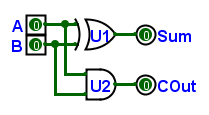
\includegraphics[width=\maxwidth{.95\linewidth}]{gfx/08_05}
	\caption{Half-Adder}
	\label{fig:08_05}
\end{figure}

\subsection{Full Adder}
\label{CL:subsec:full_adder}

A full adder sums two one-bit numbers along with a carry-in bit and produces a sum with a carry-out bit. Truth table \ref{CL:tab:truth_table_for_full_adder} defines a full adder. 

\begin{table}[H]
  \sffamily
  \newcommand{\head}[1]{\textcolor{white}{\textbf{#1}}}    
  \begin{center}
    \rowcolors{2}{gray!10}{white} % Color every other line a light gray
    \begin{tabular}{ccc|cc} 
      \rowcolor{black!75}
      \multicolumn{3}{c}{\head{Inputs}} & \multicolumn{2}{c}{\head{Output}} \\
      A & B & CIn & Sum & COut \\
      \hline
      0 & 0 & 0 & 0 & 0 \\
      0 & 0 & 1 & 1 & 0 \\
      0 & 1 & 0 & 1 & 0 \\
      0 & 1 & 1 & 0 & 1 \\
      1 & 0 & 0 & 1 & 0 \\
      1 & 0 & 1 & 0 & 1 \\
      1 & 1 & 0 & 0 & 1 \\
      1 & 1 & 1 & 1 & 1
    \end{tabular}
  \end{center}
  \caption{Truth Table for Full Adder}
  \label{CL:tab:truth_table_for_full_adder}
\end{table}

Following are Karnaugh Maps for both outputs.

%%%%%%%%%%%%%%%%%%%%%%%%%%%%%%%%%%%%%%%%%%%%%%%
%%% K-Map for Sum
%%%%%%%%%%%%%%%%%%%%%%%%%%%%%%%%%%%%%%%%%%%%%%%
\begin{figure}[H]
	\myfloatalign
	\begin{tikzpicture} [circuit logic US, scale=1.00]
	% make all path lines (the node shapes) a little thicker
	\tikzstyle{every path}=[line width=0.50mm]
	
	%********************************************************************
	% Adjust the settings below to display the 1's and rectangles
	%********************************************************************
	% Uncomment the appropriate lines below to insert ones where needed
	%   \node[] at (2.25,2.25) {\Huge $ 1 $}; % 00
	   \node[] at (2.25,0.75) {\Huge $ 1 $}; % 01
	   \node[] at (3.75,2.25) {\Huge $ 1 $}; % 02
	%   \node[] at (3.75,0.75) {\Huge $ 1 $}; % 03
	   \node[] at (6.75,2.25) {\Huge $ 1 $}; % 04
	%   \node[] at (6.75,0.75) {\Huge $ 1 $}; % 05
	%   \node[] at (5.25,2.25) {\Huge $ 1 $}; % 06
	   \node[] at (5.25,0.75) {\Huge $ 1 $}; % 07
	
	% The coords for each cell - this is used as the origin for the solution box
	\coordinate (cell00) at (1.5,1.5); \coordinate (cell01) at (1.5,0.0);
	\coordinate (cell02) at (3.0,1.5); \coordinate (cell03) at (3.0,0.0);
	
	\coordinate (cell04) at (6.0,1.5); \coordinate (cell05) at (6.0,0.0);
	\coordinate (cell06) at (4.5,1.5); \coordinate (cell07) at (4.5,0.0);
	
	% The colored boxes enclosing adjacent ones
	% Set the ``at'' to the lower-left cell of the rectangle using 
	% the 'cellxx' defined above
	% Set the minimum height/width to (number of cells) * 1.5. 
	% May have to decrease these by 0.1 to cut the rectangle 
	% just inside the cell.
	\node [draw,
	color=yellow!70!black,
	fill=yellow!20!white,
	fill opacity=0.3,
	minimum height=1.4cm,
	minimum width=1.4cm,
	double,
	rounded corners,
	anchor=south west] at (cell01) {};
	
	\node [draw,
	color=yellow!70!black,
	fill=yellow!20!white,
	fill opacity=0.3,
	minimum height=1.4cm,
	minimum width=1.4cm,
	double,
	rounded corners,
	anchor=south west] at (cell02) {};

	\node [draw,
	color=yellow!70!black,
	fill=yellow!20!white,
	fill opacity=0.3,
	minimum height=1.4cm,
	minimum width=1.4cm,
	double,
	rounded corners,
	anchor=south west] at (cell07) {};

	\node [draw,
	color=yellow!70!black,
	fill=yellow!20!white,
	fill opacity=0.3,
	minimum height=1.4cm,
	minimum width=1.4cm,
	double,
	rounded corners,
	anchor=south west] at (cell04) {};

	%********************************************************************
	% Shouldn't need to adjust anything below this point - this is just
	% the grid and the minterms.
	%********************************************************************  
	% Text in top-Left cell
	\node[] at (0.50,3.40) { $ \mathsf{ \mathbf{C} } $ }; % C
	\node[] at (1.10,4.05) { $ \mathsf{ \mathbf{AB} } $ }; % AB
	
	% Populate the top row header
	% In the following, the foreach lists a location/text pair
	% The the draw line draws the text at each location
	\foreach \loc/\txt in {
		(2.25,3.75)/{00}, (3.75,3.75)/{01},
		(5.25,3.75)/{11}, (6.75,3.75)/{10}
	}
	\draw \loc node{\Huge $\txt$};
	
	% Populate the header in column one
	\foreach \loc/\txt in { 
		(0.75,2.25)/{0},(0.75,0.75)/{1}
	}
	\draw \loc node{\Huge $\txt$};
	
	% Populate the minterms
	\foreach \loc/\txt in { 
		(2.75,1.75)/{00} , (4.25,1.75)/{02} , (5.75,1.75)/{06} , (7.25,1.75)/{04} ,
		(2.75,0.15)/{01} , (4.25,0.15)/{03} , (5.75,0.15)/{07} , (7.25,0.15)/{05} }
	\draw \loc node{ \color{blue!90!black} \small { $\txt$ }};
	
	% Draw the lines
	\draw
	% Finish drawing the grid
	[step=1.5cm,black,thin] (0,0) grid (7.5,4.5) % The Grid
	(0.0,4.5) -- (1.5,3.0) % Diagonal in the top left cell
	(1.5,3.10) -- (7.5,3.10) % Double line under top header row
	(1.40,0.0) -- (1.40,3.0) % Double line on left of header column one
	;    
	\end{tikzpicture}
	\caption{K-Map For The SUM Output}
	\label{kmap:08_01}
\end{figure}



%%%%%%%%%%%%%%%%%%%%%%%%%%%%%%%%%%%%%%%%%%%%%%%
%%% K-Map for COut
%%%%%%%%%%%%%%%%%%%%%%%%%%%%%%%%%%%%%%%%%%%%%%%
\begin{figure}[H]
	\myfloatalign
	\begin{tikzpicture} [circuit logic US, scale=1.00]
	% make all path lines (the node shapes) a little thicker
	\tikzstyle{every path}=[line width=0.50mm]
	
	%********************************************************************
	% Adjust the settings below to display the 1's and rectangles
	%********************************************************************
	% Uncomment the appropriate lines below to insert ones where needed
	%   \node[] at (2.25,2.25) {\Huge $ 1 $}; % 00
	%   \node[] at (2.25,0.75) {\Huge $ 1 $}; % 01
	%   \node[] at (3.75,2.25) {\Huge $ 1 $}; % 02
	   \node[] at (3.75,0.75) {\Huge $ 1 $}; % 03
	%   \node[] at (6.75,2.25) {\Huge $ 1 $}; % 04
	   \node[] at (6.75,0.75) {\Huge $ 1 $}; % 05
	   \node[] at (5.25,2.25) {\Huge $ 1 $}; % 06
	   \node[] at (5.25,0.75) {\Huge $ 1 $}; % 07
	
	% The coords for each cell - this is used as the origin for the solution box
	\coordinate (cell00) at (1.5,1.5); \coordinate (cell01) at (1.5,0.0);
	\coordinate (cell02) at (3.0,1.5); \coordinate (cell03) at (3.0,0.0);
	
	\coordinate (cell04) at (6.0,1.5); \coordinate (cell05) at (6.0,0.0);
	\coordinate (cell06) at (4.5,1.5); \coordinate (cell07) at (4.5,0.0);
	
	% The colored boxes enclosing adjacent ones
	% Set the ``at'' to the lower-left cell of the rectangle using 
	% the 'cellxx' defined above
	% Set the minimum height/width to (number of cells) * 1.5. 
	% May have to decrease these by 0.1 to cut the rectangle 
	% just inside the cell.
	\node [draw,
	color=red!70!black,
	fill=red!20!white,
	fill opacity=0.3,
	minimum height=1.4cm,
	minimum width=2.9cm,
	double,
	rounded corners,
	anchor=south west] at (cell03) {};

	\node [draw,
	color=green!70!black,
	fill=green!20!white,
	fill opacity=0.3,
	minimum height=1.4cm,
	minimum width=2.9cm,
	double,
	rounded corners,
	anchor=south west] at (cell07) {};
	
	\node [draw,
	color=blue!70!black,
	fill=blue!20!white,
	fill opacity=0.3,
	minimum height=2.9cm,
	minimum width=1.5cm,
	double,
	rounded corners,
	anchor=south west] at (cell07) {};
	
	%********************************************************************
	% Shouldn't need to adjust anything below this point - this is just
	% the grid and the minterms.
	%********************************************************************  
	% Text in top-Left cell
	\node[] at (0.50,3.40) { $ \mathsf{ \mathbf{C} } $ }; % C
	\node[] at (1.10,4.05) { $ \mathsf{ \mathbf{AB} } $ }; % AB
	
	% Populate the top row header
	% In the following, the foreach lists a location/text pair
	% The the draw line draws the text at each location
	\foreach \loc/\txt in {
		(2.25,3.75)/{00}, (3.75,3.75)/{01},
		(5.25,3.75)/{11}, (6.75,3.75)/{10}
	}
	\draw \loc node{\Huge $\txt$};
	
	% Populate the header in column one
	\foreach \loc/\txt in { 
		(0.75,2.25)/{0},(0.75,0.75)/{1}
	}
	\draw \loc node{\Huge $\txt$};
	
	% Populate the minterms
	\foreach \loc/\txt in { 
		(2.75,1.75)/{00} , (4.25,1.75)/{02} , (5.75,1.75)/{06} , (7.25,1.75)/{04} ,
		(2.75,0.15)/{01} , (4.25,0.15)/{03} , (5.75,0.15)/{07} , (7.25,0.15)/{05} }
	\draw \loc node{ \color{blue!90!black} \small { $\txt$ }};
	
	% Draw the lines
	\draw
	% Finish drawing the grid
	[step=1.5cm,black,thin] (0,0) grid (7.5,4.5) % The Grid
	(0.0,4.5) -- (1.5,3.0) % Diagonal in the top left cell
	(1.5,3.10) -- (7.5,3.10) % Double line under top header row
	(1.40,0.0) -- (1.40,3.0) % Double line on left of header column one
	;    
	\end{tikzpicture}
	\caption{K-Map For The COut Output}
	\label{kmap:08_02}
\end{figure}

Karnaugh map \ref{kmap:08_01} is a Reed-Muller pattern that is typical of an \textsf{XOR} gate. Karnaugh map \ref{kmap:08_02} can be reduced to three Boolean expressions. The full adder circuit is, therefore, defined by the following Boolean equations. 

\begin{align}
  \label{CL:eq:full_adder}
  A \oplus B \oplus CIn &= Sum \\
  \nonumber
  (A * B) + (A * CIn) + (B * CIn) &= COut
\end{align}

Figure \ref{fig:08_06} is a full adder. In essence, this circuit combines two half-adders such that \textsf{U1} and \textsf{U2} are one half-adder that sums \emph{A} and \emph{B} while \textsf{U3} and \textsf{U4} are the other half-adder that sums the output of the first half-adder and \emph{CIn}.

\begin{figure}[H]
	\centering
	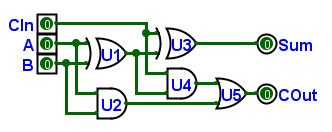
\includegraphics[width=\maxwidth{.95\linewidth}]{gfx/08_06}
	\caption{Full Adder}
	\label{fig:08_06}
\end{figure}

\subsection{Cascading Adders}
\label{CL:subsec:cascading_adders}

The full adder developed above will only add two one-bit numbers along with an optional carry-in bit; however, those adders can be cascaded such that an adder of any bit width can be easily created. Figure \ref{fig:08_07} shows a four-bit adder created by cascading four one-bit adders. 

\begin{figure}[H]
	\centering
	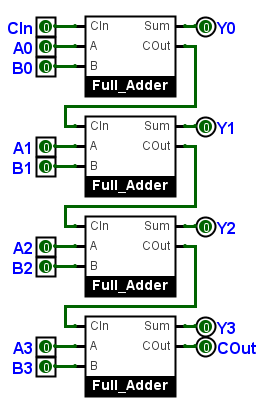
\includegraphics[width=\maxwidth{.95\linewidth}]{gfx/08_07}
	\caption{4-Bit Adder}
	\label{fig:08_07}
\end{figure}

This circuit would add two four-bit inputs, \emph{A} and \emph{B}. Stage zero, at the top of the stack, adds bit zero from both inputs and then outputs bit zero of the sum, \emph{Y0}, along with a carry-out bit. The carry-out bit from stage zero is wired directly into the stage one's carry-in port. That adder then adds bit one from both inputs along with the carry-in bit to create bit one of the sum, \emph{Y1}, along with a carry-out bit. This process continues until all for bits have been added. In the end, outputs \emph{Y0} - \emph{Y3} are combined to create a four-bit sum. If there is a carry-out bit from the last stage it could be used as the carry-in bit for another device or could be used to signal an overflow error.

\subsection{Half Subtractor}
\label{CL:subsec:half_subtractor}

To understand a binary subtraction circuit, it is helpful begin with subtraction in a base-10 system.  

\begin{binDisp}[commandchars=~\[\]]
     83
    -~underline[65]
     18
\end{binDisp}

Since $ 5 $ cannot be subtracted from $ 3 $ (the least significant digits), $ 10 $ must be borrowed from $ 8 $. This is simple elementary-school arithmetic but the principle is important for base-2 subtraction. There are only four possible one-bit subtraction problems.

\begin{binDisp}[commandchars=~\[\]]
     0     1     1     10
    -~underline[0]    -~underline[0]    -~underline[1]     -~underline[1]
     0     1     0      1
\end{binDisp}

The first three examples above need no explanation, but the fourth only makes sense when it is understood that it is impossible to subtract $ 1 $ from $ 0 $ so $ 10_{2} $ was borrowed from the next most significant bit position. The problems above were used to generate the following half-subtractor truth table.

\begin{table}[H]
	\sffamily
	\newcommand{\head}[1]{\textcolor{white}{\textbf{#1}}}    
	\begin{center}
		\rowcolors{2}{gray!10}{white} % Color every other line a light gray
		\begin{tabular}{ccc|cc} 
			\rowcolor{black!75}
			\multicolumn{2}{c}{\head{Inputs}} & \multicolumn{2}{c}{\head{Outputs}} \\
			A & B & Diff & BOut \\
			\hline
			0 & 0 & 0 & 0 \\
			0 & 1 & 1 & 1 \\
			1 & 0 & 1 & 0 \\
			1 & 1 & 0 & 0
		\end{tabular}
	\end{center}
	\caption{Truth Table for Half-Subtractor}
	\label{CL:tab:truth_table_for_half_subtractor}
\end{table}

\emph{Diff} is the difference of \emph{A} minus \emph{B}. \emph{BOut} (``Borrow Out'') is a signal that a borrow is necessary from the next most significant bit position when \emph{B} is greater than \emph{A}. The following Boolean equations define the calculations needed for a half-subtractor.

\begin{align}
\label{CL:eq:half_subtractor}
	A \oplus B &= Diff \\
	\nonumber
	A' * B &= BOut
\end{align}

The pattern for \emph{Diff} is the same as an \textsf{XOR} gate so using an \textsf{XOR} gate is the easiest way to generate the difference. \emph{BOut} is only high when \emph{A} is low and \emph{B} is high so a simple \textsf{AND} gate with one inverted input can be used to generate \emph{BOut}. The circuit in figure \ref{fig:08_08} realizes a half-subtractor.

\begin{figure}[H]
	\centering
	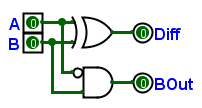
\includegraphics[width=\maxwidth{.95\linewidth}]{gfx/08_08}
	\caption{Half-Subtractor}
	\label{fig:08_08}
\end{figure}

\subsection{Full Subtractor}
\label{CL:subsec:full_subtractor}

A full subtractor produces a difference and borrow-out signal, just like a half-subtractor, but also includes a borrow-in signal so they can be cascaded to create a subtractor of any desired bit width.

Truth table \ref{CL:tab:truth_table_for_subtractor} is for a full subtractor. 

\begin{table}[H]
	\sffamily
	\newcommand{\head}[1]{\textcolor{white}{\textbf{#1}}}    
	\begin{center}
		\rowcolors{2}{gray!10}{white} % Color every other line a light gray
		\begin{tabular}{ccc|cc} 
			\rowcolor{black!75}
			\multicolumn{3}{c}{\head{Inputs}} & \multicolumn{2}{c}{\head{Output}} \\
			A & B & BIn & Diff & BOut \\
			\hline
			0 & 0 & 0 & 0 & 0 \\
			0 & 0 & 1 & 1 & 1 \\
			0 & 1 & 0 & 1 & 1 \\
			0 & 1 & 1 & 0 & 1 \\
			1 & 0 & 0 & 1 & 0 \\
			1 & 0 & 1 & 0 & 0 \\
			1 & 1 & 0 & 0 & 0 \\
			1 & 1 & 1 & 1 & 1
		\end{tabular}
	\end{center}
	\caption{Truth Table for Subtractor}
	\label{CL:tab:truth_table_for_subtractor}
\end{table}

\emph{Diff} is the difference of \emph{A} minus \emph{B} minus \emph{BIn}. \emph{BOut} (``Borrow Out'') is a signal that a borrow is necessary from the next most significant bit position when \emph{A} is less than \emph{B} plus \emph{BIn}. 

Following are Karnaugh Maps for both outputs.

%%%%%%%%%%%%%%%%%%%%%%%%%%%%%%%%%%%%%%%%%%%%%%%
%%% K-Map for Difference
%%%%%%%%%%%%%%%%%%%%%%%%%%%%%%%%%%%%%%%%%%%%%%%
\begin{figure}[H]
	\myfloatalign
	\begin{tikzpicture} [circuit logic US, scale=1.00]
	% make all path lines (the node shapes) a little thicker
	\tikzstyle{every path}=[line width=0.50mm]
	
	%********************************************************************
	% Adjust the settings below to display the 1's and rectangles
	%********************************************************************
	% Uncomment the appropriate lines below to insert ones where needed
	%   \node[] at (2.25,2.25) {\Huge $ 1 $}; % 00
	\node[] at (2.25,0.75) {\Huge $ 1 $}; % 01
	\node[] at (3.75,2.25) {\Huge $ 1 $}; % 02
	%   \node[] at (3.75,0.75) {\Huge $ 1 $}; % 03
	\node[] at (6.75,2.25) {\Huge $ 1 $}; % 04
	%   \node[] at (6.75,0.75) {\Huge $ 1 $}; % 05
	%   \node[] at (5.25,2.25) {\Huge $ 1 $}; % 06
	\node[] at (5.25,0.75) {\Huge $ 1 $}; % 07
	
	% The coords for each cell - this is used as the origin for the solution box
	\coordinate (cell00) at (1.5,1.5); \coordinate (cell01) at (1.5,0.0);
	\coordinate (cell02) at (3.0,1.5); \coordinate (cell03) at (3.0,0.0);
	
	\coordinate (cell04) at (6.0,1.5); \coordinate (cell05) at (6.0,0.0);
	\coordinate (cell06) at (4.5,1.5); \coordinate (cell07) at (4.5,0.0);
	
	% The colored boxes enclosing adjacent ones
	% Set the ``at'' to the lower-left cell of the rectangle using 
	% the 'cellxx' defined above
	% Set the minimum height/width to (number of cells) * 1.5. 
	% May have to decrease these by 0.1 to cut the rectangle 
	% just inside the cell.
	\node [draw,
	color=yellow!70!black,
	fill=yellow!20!white,
	fill opacity=0.3,
	minimum height=1.4cm,
	minimum width=1.4cm,
	double,
	rounded corners,
	anchor=south west] at (cell01) {};
	
	\node [draw,
	color=yellow!70!black,
	fill=yellow!20!white,
	fill opacity=0.3,
	minimum height=1.4cm,
	minimum width=1.4cm,
	double,
	rounded corners,
	anchor=south west] at (cell02) {};
	
	\node [draw,
	color=yellow!70!black,
	fill=yellow!20!white,
	fill opacity=0.3,
	minimum height=1.4cm,
	minimum width=1.4cm,
	double,
	rounded corners,
	anchor=south west] at (cell07) {};
	
	\node [draw,
	color=yellow!70!black,
	fill=yellow!20!white,
	fill opacity=0.3,
	minimum height=1.4cm,
	minimum width=1.4cm,
	double,
	rounded corners,
	anchor=south west] at (cell04) {};
	
	%********************************************************************
	% Shouldn't need to adjust anything below this point - this is just
	% the grid and the minterms.
	%********************************************************************  
	% Text in top-Left cell
	\node[] at (0.50,3.40) { $ \mathsf{ \mathbf{C} } $ }; % C
	\node[] at (1.10,4.05) { $ \mathsf{ \mathbf{AB} } $ }; % AB
	
	% Populate the top row header
	% In the following, the foreach lists a location/text pair
	% The the draw line draws the text at each location
	\foreach \loc/\txt in {
		(2.25,3.75)/{00}, (3.75,3.75)/{01},
		(5.25,3.75)/{11}, (6.75,3.75)/{10}
	}
	\draw \loc node{\Huge $\txt$};
	
	% Populate the header in column one
	\foreach \loc/\txt in { 
		(0.75,2.25)/{0},(0.75,0.75)/{1}
	}
	\draw \loc node{\Huge $\txt$};
	
	% Populate the minterms
	\foreach \loc/\txt in { 
		(2.75,1.75)/{00} , (4.25,1.75)/{02} , (5.75,1.75)/{06} , (7.25,1.75)/{04} ,
		(2.75,0.15)/{01} , (4.25,0.15)/{03} , (5.75,0.15)/{07} , (7.25,0.15)/{05} }
	\draw \loc node{ \color{blue!90!black} \small { $\txt$ }};
	
	% Draw the lines
	\draw
	% Finish drawing the grid
	[step=1.5cm,black,thin] (0,0) grid (7.5,4.5) % The Grid
	(0.0,4.5) -- (1.5,3.0) % Diagonal in the top left cell
	(1.5,3.10) -- (7.5,3.10) % Double line under top header row
	(1.40,0.0) -- (1.40,3.0) % Double line on left of header column one
	;    
	\end{tikzpicture}
	\caption{K-Map For The Difference Output}
	\label{kmap:08_03}
\end{figure}



%%%%%%%%%%%%%%%%%%%%%%%%%%%%%%%%%%%%%%%%%%%%%%%
%%% K-Map for BOut
%%%%%%%%%%%%%%%%%%%%%%%%%%%%%%%%%%%%%%%%%%%%%%%
\begin{figure}[H]
	\myfloatalign
	\begin{tikzpicture} [circuit logic US, scale=1.00]
	% make all path lines (the node shapes) a little thicker
	\tikzstyle{every path}=[line width=0.50mm]
	
	%********************************************************************
	% Adjust the settings below to display the 1's and rectangles
	%********************************************************************
	% Uncomment the appropriate lines below to insert ones where needed
	%   \node[] at (2.25,2.25) {\Huge $ 1 $}; % 00
	   \node[] at (2.25,0.75) {\Huge $ 1 $}; % 01
	   \node[] at (3.75,2.25) {\Huge $ 1 $}; % 02
	   \node[] at (3.75,0.75) {\Huge $ 1 $}; % 03
	%   \node[] at (6.75,2.25) {\Huge $ 1 $}; % 04
	%   \node[] at (6.75,0.75) {\Huge $ 1 $}; % 05
	%   \node[] at (5.25,2.25) {\Huge $ 1 $}; % 06
	   \node[] at (5.25,0.75) {\Huge $ 1 $}; % 07
	
	% The coords for each cell - this is used as the origin for the solution box
	\coordinate (cell00) at (1.5,1.5); \coordinate (cell01) at (1.5,0.0);
	\coordinate (cell02) at (3.0,1.5); \coordinate (cell03) at (3.0,0.0);
	
	\coordinate (cell04) at (6.0,1.5); \coordinate (cell05) at (6.0,0.0);
	\coordinate (cell06) at (4.5,1.5); \coordinate (cell07) at (4.5,0.0);
	
	% The colored boxes enclosing adjacent ones
	% Set the ``at'' to the lower-left cell of the rectangle using 
	% the 'cellxx' defined above
	% Set the minimum height/width to (number of cells) * 1.5. 
	% May have to decrease these by 0.1 to cut the rectangle 
	% just inside the cell.
	\node [draw,
	color=red!70!black,
	fill=red!20!white,
	fill opacity=0.3,
	minimum height=1.4cm,
	minimum width=2.9cm,
	double,
	rounded corners,
	anchor=south west] at (cell01) {};
	
	\node [draw,
	color=green!70!black,
	fill=green!20!white,
	fill opacity=0.3,
	minimum height=1.4cm,
	minimum width=2.9cm,
	double,
	rounded corners,
	anchor=south west] at (cell03) {};
	
	\node [draw,
	color=blue!70!black,
	fill=blue!20!white,
	fill opacity=0.3,
	minimum height=2.9cm,
	minimum width=1.5cm,
	double,
	rounded corners,
	anchor=south west] at (cell03) {};
	
	%********************************************************************
	% Shouldn't need to adjust anything below this point - this is just
	% the grid and the minterms.
	%********************************************************************  
	% Text in top-Left cell
	\node[] at (0.50,3.40) { $ \mathsf{ \mathbf{C} } $ }; % C
	\node[] at (1.10,4.05) { $ \mathsf{ \mathbf{AB} } $ }; % AB
	
	% Populate the top row header
	% In the following, the foreach lists a location/text pair
	% The the draw line draws the text at each location
	\foreach \loc/\txt in {
		(2.25,3.75)/{00}, (3.75,3.75)/{01},
		(5.25,3.75)/{11}, (6.75,3.75)/{10}
	}
	\draw \loc node{\Huge $\txt$};
	
	% Populate the header in column one
	\foreach \loc/\txt in { 
		(0.75,2.25)/{0},(0.75,0.75)/{1}
	}
	\draw \loc node{\Huge $\txt$};
	
	% Populate the minterms
	\foreach \loc/\txt in { 
		(2.75,1.75)/{00} , (4.25,1.75)/{02} , (5.75,1.75)/{06} , (7.25,1.75)/{04} ,
		(2.75,0.15)/{01} , (4.25,0.15)/{03} , (5.75,0.15)/{07} , (7.25,0.15)/{05} }
	\draw \loc node{ \color{blue!90!black} \small { $\txt$ }};
	
	% Draw the lines
	\draw
	% Finish drawing the grid
	[step=1.5cm,black,thin] (0,0) grid (7.5,4.5) % The Grid
	(0.0,4.5) -- (1.5,3.0) % Diagonal in the top left cell
	(1.5,3.10) -- (7.5,3.10) % Double line under top header row
	(1.40,0.0) -- (1.40,3.0) % Double line on left of header column one
	;    
	\end{tikzpicture}
	\caption{K-Map For The BOut Output}
	\label{kmap:08_04}
\end{figure}

Karnaugh map \ref{kmap:08_03} is a Reed-Muller pattern that is typical of an \textsf{XOR} gate. Karnaugh map \ref{kmap:08_04} can be reduced to three Boolean expressions. The full subtactor circuit is, therefore, defined by the following Boolean equations. 

\begin{align}
	\label{CL:eq:subtractor}
	A \oplus B \oplus BIn &= Diff \\
	\nonumber
	A'B + (A' * BIn) + (B * BIn) &= BOut
\end{align}

The circuit in figure \ref{fig:08_09} realizes a subtractor.

\begin{figure}[H]
	\centering
	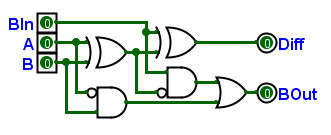
\includegraphics[width=\maxwidth{.95\linewidth}]{gfx/08_09}
	\caption{Subtractor}
	\label{fig:08_09}
\end{figure}

\subsection{Cascading Subtractors}
\label{CL:subsec:cascading_subtractors}

The full subtractor developed above will only subtract two one-bit numbers along with an optional borrow bit; however, those subtractors can be cascaded such that a subtractor of any bit width can be easily created. Figure \ref{fig:08_10} shows a four-bit subtractor created by cascading four one-bit subtractors.

\begin{figure}[H]
	\centering
	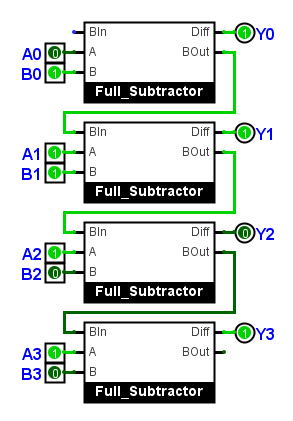
\includegraphics[width=\maxwidth{.95\linewidth}]{gfx/08_10}
	\caption{4-Bit Subtractor}
	\label{fig:08_10}
\end{figure}

This circuit would subtract a four bit number \emph{B} from \emph{A}. The subtractor is set up to solve $ 1110_2 - 0011_2 = 1011_2 $. Stage zero, at the top of the stack, subtracts bit zero of input \emph{B} from bit zero of input \emph{A} and then outputs bit zero of the difference, \emph{Y0}, along with a borrow-out bit. The borrow-out bit from stage zero is wired directly into the stage one's borrow-in port. That stage then subtracts bit one of input \emph{B} from bit one of input \emph{A} along with the borrow-in bit to create bit one of the sum, \emph{Y1}, along with a borrow-out bit. This process continues until all for bits have been subtracted. In the end, outputs \emph{Y0} - \emph{Y3} are combined to create a four-bit difference. The borrow-out bit of the last stage is not connected to anything but it could be used as the borrow-in bit for another device.

\subsection{Adder-Subtractor Circuit}
\label{CL:subsec:adder_subtractor_circuit}

It is remarkably easy to create a device that both adds and subtracts based on a single-bit control signal. Figure \ref{fig:08_11} is a 4-bit adder that was modified to become both an adder and subtractor. The circuit has been set up with this problem: $ 0101_2 - 0011_2 = 0010_2 $. 

\begin{figure}[H]
	\centering
	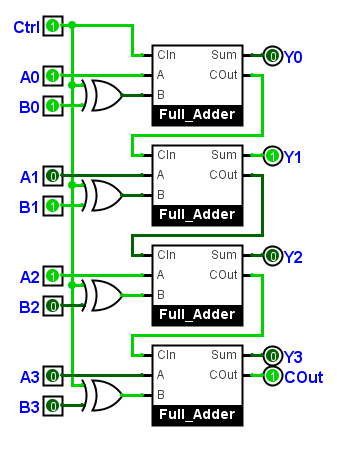
\includegraphics[width=\maxwidth{.95\linewidth}]{gfx/08_11}
	\caption{4-Bit Adder-Subtractor}
	\label{fig:08_11}
\end{figure}

To change an adder to an adder-subtractor makes use of the binary mathematics concept of subtracting by adding the twos complement (see Section \ref{MO:subsub:binary_subtraction_with_radix_complement} on page \pageref{MO:subsub:binary_subtraction_with_radix_complement}). The ``trick'' is to use the \textsf{XOR} gates on input \emph{B} to convert that input to its complement then the adder will subtract \emph{B} from \emph{A} instead of add. 

To create the twos complement of a binary number each of the bits are complemented and then one is added to the result (again, this process is described in Section \ref{MO:subsub:binary_subtraction_with_radix_complement}). Each of the \emph{B} input bits are wired through one input of an \textsf{XOR} gate. The other input of that gate is a \emph{Ctrl} (``Control'') bit. When \emph{Ctrl} is low then each of the \emph{B} inputs are transmitted through an \textsf{XOR} gate without change and the adder works as an adder. When \emph{Ctrl} is high then each of the \emph{B} inputs are complemented by an \textsf{XOR} gate such that the ones complement is created. However, \emph{Ctrl} is also wired to the \emph{CIn} input of the first stage which has the effect of adding one to the result and turn input \emph{B} into a twos complement number. Now the adder will subtract input \emph{B} from input \emph{A}.

In the end, the designer only needs to set \emph{Ctrl} to zero to make the circuit add or one to make the circuit subtract.

\subsection{Integrated Circuits}
\label{CL:subsec:adder_integrated_circuits}

In practice, circuit designers rarely build adders or subtractors. There are many different types of manufactured low-cost adders, subtractors, and adder/subtractor combinations available and designers usually find it easiest to use one of those circuits rather than re-invent the proverbial wheel. A quick look at Wikipedia\footnote{\url{https://www.wikipedia.com/en/List_of_7400_series_integrated_circuits}} found this list of adders:

\begin{itemize}
	\item $ 7480 $, gated full adder
	\item $ 7482 $, two-bit binary full adder
	\item $ 7483 $, four-bit binary full adder
	\item $ 74183 $, dual carry-save full adder
	\item $ 74283 $, four-bit binary full adder
	\item $ 74385 $, quad four-bit adder/subtractor
	\item $ 74456 $, BCD adder
\end{itemize}

In addition to adder circuits, designers can also opt to use an \gls{alu} \gls{ic}.

\section{Arithmetic Logic Units}
\label{CL:sec:arithmetic_and_logic_units}

An \gls{alu} is a specialized \gls{ic} that performs all arithmetic and logic functions needed in a device. Most \glspl{alu} will carry out dozens of different functions like the following few examples from a $ 74181 $ \gls{alu} (assume that the ALU has two inputs, $ A $ and $ B $, and one output, $ F $):

\begin{itemize}
  \item \lstinline[columns=fixed]|F = NOT A|
  \item \lstinline[columns=fixed]|F = A NAND B|
  \item \lstinline[columns=fixed]|F = (NOT A) OR B|
  \item \lstinline[columns=fixed]|F = B|
  \item \lstinline[columns=fixed]|F = (NOT A) AND B|
  \item \lstinline[columns=fixed]|F = A - 1|
  \item \lstinline[columns=fixed]|F = A - B|
  \item \lstinline[columns=fixed]|F = AB - 1|
  \item \lstinline[columns=fixed]|F = -1|
\end{itemize}

\glspl{alu} are very important in many devices, in fact, they are at the core of a \gls{cpu}. Because they are readily available at low cost, most designers will use a commercially-produced \gls{alu} in a project rather than try to create their own.

A quick look at Wikipedia\footnote{\url{https://www.wikipedia.com/en/List_of_7400_series_integrated_circuits}} found this list of \glspl{alu}:

\begin{itemize}
  \item $ 74181 $, four-bit arithmetic logic unit and function generator
  \item $ 74381 $, four-bit arithmetic logic unit/function generator with generate and propagate outputs
  \item $ 74382 $, four-bit arithmetic logic unit/function generator with ripple carry and overflow outputs
  \item $ 74881 $, Arithmetic logic unit
\end{itemize}

\section{Comparators}
\label{CL:sec:comparators}

A comparator compares two binary numbers, \emph{A} and \emph{B}. One of three outputs is generated by the comparison: \lstinline[]|A = B, A > B, A < B|. A one-bit comparator uses a combination of \textsf{AND} gates, \textsf{NOT} gates, and an \textsf{XNOR} gate to generate a \emph{True} output for each of the three comparisons: 

\begin{table}[H]
	\sffamily
	\newcommand{\head}[1]{\textcolor{white}{\textbf{#1}}}    
	\begin{center}
		\rowcolors{1}{gray!10}{white} % Color every other line a light gray
		\begin{tabular}{cc} 
			$ A=B $ & $ (A \odot B)' $ \\
			$ A > B $ & $ AB' $ \\
			$ A < B $ & $ A'B $
		\end{tabular}
	\end{center}
	\caption{One-Bit Comparator Functions}
	\label{CL:tab:one-bit_comparator_functions}
\end{table}

Figure \ref{fig:08_12} is the logic diagram for a one-bit comparator.  

\begin{figure}[H]
	\centering
	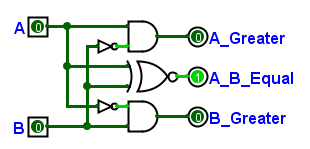
\includegraphics[width=\maxwidth{.95\linewidth}]{gfx/08_12}
	\caption{One-Bit Comparator}
	\label{fig:08_12}
\end{figure}

To compare numbers larger than one bit requires a more involved analysis of the problem. First, a truth table is developed for every possible combination of two 2-bit numbers, \emph{A} and \emph{B}.

\begin{table}[H]
	\sffamily
	\newcommand{\head}[1]{\textcolor{white}{\textbf{#1}}}		
	\begin{center}
		\rowcolors{2}{gray!10}{white} % Color every other line a light gray
		\begin{tabular}{cccc|ccc} 
			\rowcolor{black!75}
			\multicolumn{4}{c}{\head{Inputs}} & \multicolumn{3}{c}{\head{Outputs}} \\
			$A1$ & $A0$ & $B1$ & $B0$ & $A<B$ & $A=B$ & $A>B$ \\
			\hline
			0 & 0 & 0 & 0 & 0 & 1 & 0 \\
			0 & 0 & 0 & 1 & 1 & 0 & 0 \\
			0 & 0 & 1 & 0 & 1 & 0 & 0 \\
			0 & 0 & 1 & 1 & 1 & 0 & 0 \\
			0 & 1 & 0 & 0 & 0 & 0 & 1 \\
			0 & 1 & 0 & 1 & 0 & 1 & 0 \\
			0 & 1 & 1 & 0 & 1 & 0 & 0 \\
			0 & 1 & 1 & 1 & 1 & 0 & 0 \\
			1 & 0 & 0 & 0 & 0 & 0 & 1 \\
			1 & 0 & 0 & 1 & 0 & 0 & 1 \\
			1 & 0 & 1 & 0 & 0 & 1 & 0 \\
			1 & 0 & 1 & 1 & 1 & 0 & 0 \\
			1 & 1 & 0 & 0 & 0 & 0 & 1 \\
			1 & 1 & 0 & 1 & 0 & 0 & 1 \\
			1 & 1 & 1 & 0 & 0 & 0 & 1 \\
			1 & 1 & 1 & 1 & 0 & 1 & 0 
		\end{tabular}
	\end{center}
	\caption{Truth Table for Two-Bit Comparator}
	\label{08:tab:two_bit_comparator}
\end{table}

Next, Karnaugh Maps are developed for each of the three outputs.

%%%%%%%%%%%%%%%%%%%%%%%%%%%%%%%%%%%%%%%%%%%%%%%%%%%%%%%%%%%%%%
% K-Map #1 A>B
%%%%%%%%%%%%%%%%%%%%%%%%%%%%%%%%%%%%%%%%%%%%%%%%%%%%%%%%%%%%%%

\begin{figure}[H]
	\myfloatalign
	\begin{tikzpicture} [circuit logic US, scale=1.00]
	% make all path lines (the node shapes) a little thicker
	\tikzstyle{every path}=[line width=0.50mm]
	
	%********************************************************************
	% Adjust the settings below to display the 1's and rectangles
	%********************************************************************
	% Uncomment the appropriate lines below to insert ones where needed
	% Data Row 1
	% \node[] at (2.25,5.25) {\Huge $ 1 $}; % 00
	% \node[] at (3.75,5.25) {\Huge $ 1 $}; % 04
	% \node[] at (5.25,5.25) {\Huge $ 1 $}; % 12
	% \node[] at (6.75,5.25) {\Huge $ 1 $}; % 08
	% Data Row 2
	\node[] at (2.25,3.75) {\Huge $ 1 $}; % 01
	% \node[] at (3.75,3.75) {\Huge $ 1 $}; % 05
	% \node[] at (5.25,3.75) {\Huge $ 1 $}; % 13
	% \node[] at (6.75,3.75) {\Huge $ 1 $}; % 09
	% Data Row 3
	\node[] at (2.25,2.25) {\Huge $ 1 $}; % 03
	\node[] at (3.75,2.25) {\Huge $ 1 $}; % 07
	% \node[] at (5.25,2.25) {\Huge $ 1 $}; % 15
	\node[] at (6.75,2.25) {\Huge $ 1 $}; % 11
	% Data Row 4
	\node[] at (2.25,0.75) {\Huge $ 1 $}; % 02
	\node[] at (3.75,0.75) {\Huge $ 1 $}; % 06
	% \node[] at (5.25,0.75) {\Huge $ 1 $}; % 14
	% \node[] at (6.75,0.75) {\Huge $ 1 $}; % 10
	
	% The coords for each cell - this is used to start the rectangle box
	\coordinate (cell00) at (1.50,4.50); \coordinate (cell01) at (1.50,3.00);
	\coordinate (cell02) at (1.50,0.00); \coordinate (cell03) at (1.50,1.50);
	\coordinate (cell04) at (3.00,4.50); \coordinate (cell05) at (3.00,3.00);
	\coordinate (cell06) at (3.00,0.00); \coordinate (cell07) at (3.00,1.50);
	\coordinate (cell08) at (6.00,4.50); \coordinate (cell09) at (6.00,3.00);
	\coordinate (cell10) at (6.00,0.00); \coordinate (cell11) at (6.00,1.50);
	\coordinate (cell12) at (4.50,4.50); \coordinate (cell13) at (4.50,3.00);
	\coordinate (cell14) at (4.50,0.00); \coordinate (cell15) at (4.50,1.50);
	
	% Set the ``at'' to the lower-left cell of the rectangle using the coords defined above
	% Set the minimum height/width to (number of cells) * 1.5. May have to decrease 
	% these by 0.1 to cut the rectangle just inside the cell.
	\node [draw,
	color=red!70!black,
	fill=red!20!white,
	fill opacity=0.3,
	minimum height=2.9cm,
	minimum width=3.0cm,
	double,
	rounded corners,
	anchor=south west] at (cell02) {};
	
	\node [draw,
	color=blue!70!black,
	fill=blue!20!white,
	fill opacity=0.3,
	minimum height=2.9cm,
	minimum width=1.5cm,
	double,
	rounded corners,
	anchor=south west] at (cell03) {};
	
	\node [draw,
	color=green!70!black,
	fill=green!20!white,
	fill opacity=0.3,
	minimum height=1.4cm,
	minimum width=1.5cm,
	double,
	rounded corners,
	anchor=south west] at (cell11) {};
	
	\node [draw,
	color=green!70!black,
	fill=green!20!white,
	fill opacity=0.3,
	minimum height=1.4cm,
	minimum width=1.5cm,
	double,
	rounded corners,
	anchor=south west] at (cell03) {};
	
	%********************************************************************
	% Shouldn't need to adjust anything below this point - this is just
	% the grid and the minterms.
	%********************************************************************	
	% Text in top-Left cell
	\node[] at (0.55,6.35) { $ \mathsf{ \mathbf{A1A0} } $ }; % CD
	\node[] at (1.05,7.05) { $ \mathsf{ \mathbf{B1B0} } $ }; % AB
	
	% Populate the top row header
	% In the following, the foreach lists a location/text pair
	% The the draw line draws the text at each location
	\foreach \loc/\txt in {(2.25,6.75)/{00},(3.75,6.75)/{01},(5.25,6.75)/{11},(6.75,6.75)/{10}}
	\draw \loc node{\Huge $\txt$};
	
	% Populate the header in column one
	\foreach \loc/\txt in {(0.75,5.25)/{00},(0.75,3.75)/{01},(0.75,2.25)/{11},(0.75,0.75)/{10}}
	\draw \loc node{\Huge $\txt$};
	
	% Populate the minterms
	\foreach \loc/\txt in { (2.75,4.75)/{00} , (4.25,4.75)/{04} , (5.75,4.75)/{12} , (7.25,4.75)/{08} ,
		(2.75,3.25)/{01} , (4.25,3.25)/{05} , (5.75,3.25)/{13} , (7.25,3.25)/{09} ,
		(2.75,1.75)/{03} , (4.25,1.75)/{07} , (5.75,1.75)/{15} , (7.25,1.75)/{11} ,
		(2.75,0.25)/{02} , (4.25,0.25)/{06} , (5.75,0.25)/{14} , (7.25,0.25)/{10} }
	\draw \loc node{ \color{blue!90!black} \small{ $\txt$ }};
	
	% Draw the lines
	\draw
	% Finish drawing the grid
	[step=1.5cm,black,thin] (0,0) grid (7.5,7.5) % The Grid
	(0.0,7.5) -- (1.5,6.0) % Diagonal in the top left cell
	(1.5,6.10) -- (7.50,6.10) % Double line under top header row
	(1.40,0.0) -- (1.40,6.0) % Double line on left of header column one
	;
	\end{tikzpicture}
	\caption{K-Map For $A>B$}
	\label{kmap:08_05}
\end{figure}

%%%%%%%%%%%%%%%%%%%%%%%%%%%%%%%%%%%%%%%%%%%%%%%%%%%%%%%%%%%%%%
% K-Map #2 A=B
%%%%%%%%%%%%%%%%%%%%%%%%%%%%%%%%%%%%%%%%%%%%%%%%%%%%%%%%%%%%%%

\begin{figure}[H]
	\myfloatalign
	\begin{tikzpicture} [circuit logic US, scale=1.00]
	% make all path lines (the node shapes) a little thicker
	\tikzstyle{every path}=[line width=0.50mm]
	
	%********************************************************************
	% Adjust the settings below to display the 1's and rectangles
	%********************************************************************
	% Uncomment the appropriate lines below to insert ones where needed
	% Data Row 1
	\node[] at (2.25,5.25) {\Huge $ 1 $}; % 00
	% \node[] at (3.75,5.25) {\Huge $ 1 $}; % 04
	% \node[] at (5.25,5.25) {\Huge $ 1 $}; % 12
	% \node[] at (6.75,5.25) {\Huge $ 1 $}; % 08
	% Data Row 2
	% \node[] at (2.25,3.75) {\Huge $ 1 $}; % 01
	\node[] at (3.75,3.75) {\Huge $ 1 $}; % 05
	% \node[] at (5.25,3.75) {\Huge $ 1 $}; % 13
	% \node[] at (6.75,3.75) {\Huge $ 1 $}; % 09
	% Data Row 3
	% \node[] at (2.25,2.25) {\Huge $ 1 $}; % 03
	% \node[] at (3.75,2.25) {\Huge $ 1 $}; % 07
	\node[] at (5.25,2.25) {\Huge $ 1 $}; % 15
	% \node[] at (6.75,2.25) {\Huge $ 1 $}; % 11
	% Data Row 4
	% \node[] at (2.25,0.75) {\Huge $ 1 $}; % 02
	% \node[] at (3.75,0.75) {\Huge $ 1 $}; % 06
	% \node[] at (5.25,0.75) {\Huge $ 1 $}; % 14
	\node[] at (6.75,0.75) {\Huge $ 1 $}; % 10
	
	% The coords for each cell - this is used to start the rectangle box
	\coordinate (cell00) at (1.50,4.50); \coordinate (cell01) at (1.50,3.00);
	\coordinate (cell02) at (1.50,0.00); \coordinate (cell03) at (1.50,1.50);
	\coordinate (cell04) at (3.00,4.50); \coordinate (cell05) at (3.00,3.00);
	\coordinate (cell06) at (3.00,0.00); \coordinate (cell07) at (3.00,1.50);
	\coordinate (cell08) at (6.00,4.50); \coordinate (cell09) at (6.00,3.00);
	\coordinate (cell10) at (6.00,0.00); \coordinate (cell11) at (6.00,1.50);
	\coordinate (cell12) at (4.50,4.50); \coordinate (cell13) at (4.50,3.00);
	\coordinate (cell14) at (4.50,0.00); \coordinate (cell15) at (4.50,1.50);
	
	% Set the ``at'' to the lower-left cell of the rectangle using the coords defined above
	% Set the minimum height/width to (number of cells) * 1.5. May have to decrease 
	% these by 0.1 to cut the rectangle just inside the cell.
	\node [draw,
	color=red!70!black,
	fill=red!20!white,
	fill opacity=0.3,
	minimum height=1.4cm,
	minimum width=1.5cm,
	double,
	rounded corners,
	anchor=south west] at (cell00) {};
	
	\node [draw,
	color=blue!70!black,
	fill=blue!20!white,
	fill opacity=0.3,
	minimum height=1.4cm,
	minimum width=1.5cm,
	double,
	rounded corners,
	anchor=south west] at (cell05) {};
	
	\node [draw,
	color=yellow!70!black,
	fill=yellow!20!white,
	fill opacity=0.3,
	minimum height=1.4cm,
	minimum width=1.5cm,
	double,
	rounded corners,
	anchor=south west] at (cell15) {};
	
	\node [draw,
	color=green!70!black,
	fill=green!20!white,
	fill opacity=0.3,
	minimum height=1.4cm,
	minimum width=1.5cm,
	double,
	rounded corners,
	anchor=south west] at (cell10) {};
	
	%********************************************************************
	% Shouldn't need to adjust anything below this point - this is just
	% the grid and the minterms.
	%********************************************************************	
	% Text in top-Left cell
	\node[] at (0.55,6.35) { $ \mathsf{ \mathbf{A1A0} } $ }; % CD
	\node[] at (1.05,7.05) { $ \mathsf{ \mathbf{B1B0} } $ }; % AB
	
	% Populate the top row header
	% In the following, the foreach lists a location/text pair
	% The the draw line draws the text at each location
	\foreach \loc/\txt in {(2.25,6.75)/{00},(3.75,6.75)/{01},(5.25,6.75)/{11},(6.75,6.75)/{10}}
	\draw \loc node{\Huge $\txt$};
	
	% Populate the header in column one
	\foreach \loc/\txt in {(0.75,5.25)/{00},(0.75,3.75)/{01},(0.75,2.25)/{11},(0.75,0.75)/{10}}
	\draw \loc node{\Huge $\txt$};
	
	% Populate the minterms
	\foreach \loc/\txt in { (2.75,4.75)/{00} , (4.25,4.75)/{04} , (5.75,4.75)/{12} , (7.25,4.75)/{08} ,
		(2.75,3.25)/{01} , (4.25,3.25)/{05} , (5.75,3.25)/{13} , (7.25,3.25)/{09} ,
		(2.75,1.75)/{03} , (4.25,1.75)/{07} , (5.75,1.75)/{15} , (7.25,1.75)/{11} ,
		(2.75,0.25)/{02} , (4.25,0.25)/{06} , (5.75,0.25)/{14} , (7.25,0.25)/{10} }
	\draw \loc node{ \color{blue!90!black} \small{ $\txt$ }};
	
	% Draw the lines
	\draw
	% Finish drawing the grid
	[step=1.5cm,black,thin] (0,0) grid (7.5,7.5) % The Grid
	(0.0,7.5) -- (1.5,6.0) % Diagonal in the top left cell
	(1.5,6.10) -- (7.50,6.10) % Double line under top header row
	(1.40,0.0) -- (1.40,6.0) % Double line on left of header column one
	;
	\end{tikzpicture}
	\caption{K-Map For $A=B$}
	\label{kmap:08_06}
\end{figure}

%%%%%%%%%%%%%%%%%%%%%%%%%%%%%%%%%%%%%%%%%%%%%%%%%%%%%%%%%%%%%%
% K-Map #3 A<B
%%%%%%%%%%%%%%%%%%%%%%%%%%%%%%%%%%%%%%%%%%%%%%%%%%%%%%%%%%%%%%

\begin{figure}[H]
	\myfloatalign
	\begin{tikzpicture} [circuit logic US, scale=1.00]
	% make all path lines (the node shapes) a little thicker
	\tikzstyle{every path}=[line width=0.50mm]
	
	%********************************************************************
	% Adjust the settings below to display the 1's and rectangles
	%********************************************************************
	% Uncomment the appropriate lines below to insert ones where needed
	% Data Row 1
	% \node[] at (2.25,5.25) {\Huge $ 1 $}; % 00
	\node[] at (3.75,5.25) {\Huge $ 1 $}; % 04
	\node[] at (5.25,5.25) {\Huge $ 1 $}; % 12
	\node[] at (6.75,5.25) {\Huge $ 1 $}; % 08
	% Data Row 2
	% \node[] at (2.25,3.75) {\Huge $ 1 $}; % 01
	% \node[] at (3.75,3.75) {\Huge $ 1 $}; % 05
	\node[] at (5.25,3.75) {\Huge $ 1 $}; % 13
	\node[] at (6.75,3.75) {\Huge $ 1 $}; % 09
	% Data Row 3
	% \node[] at (2.25,2.25) {\Huge $ 1 $}; % 03
	% \node[] at (3.75,2.25) {\Huge $ 1 $}; % 07
	% \node[] at (5.25,2.25) {\Huge $ 1 $}; % 15
	% \node[] at (6.75,2.25) {\Huge $ 1 $}; % 11
	% Data Row 4
	% \node[] at (2.25,0.75) {\Huge $ 1 $}; % 02
	% \node[] at (3.75,0.75) {\Huge $ 1 $}; % 06
	\node[] at (5.25,0.75) {\Huge $ 1 $}; % 14
	% \node[] at (6.75,0.75) {\Huge $ 1 $}; % 10
	
	% The coords for each cell - this is used to start the rectangle box
	\coordinate (cell00) at (1.50,4.50); \coordinate (cell01) at (1.50,3.00);
	\coordinate (cell02) at (1.50,0.00); \coordinate (cell03) at (1.50,1.50);
	\coordinate (cell04) at (3.00,4.50); \coordinate (cell05) at (3.00,3.00);
	\coordinate (cell06) at (3.00,0.00); \coordinate (cell07) at (3.00,1.50);
	\coordinate (cell08) at (6.00,4.50); \coordinate (cell09) at (6.00,3.00);
	\coordinate (cell10) at (6.00,0.00); \coordinate (cell11) at (6.00,1.50);
	\coordinate (cell12) at (4.50,4.50); \coordinate (cell13) at (4.50,3.00);
	\coordinate (cell14) at (4.50,0.00); \coordinate (cell15) at (4.50,1.50);
	
	% Set the ``at'' to the lower-left cell of the rectangle using the coords defined above
	% Set the minimum height/width to (number of cells) * 1.5. May have to decrease 
	% these by 0.1 to cut the rectangle just inside the cell.
	\node [draw,
	color=red!70!black,
	fill=red!20!white,
	fill opacity=0.3,
	minimum height=2.9cm,
	minimum width=3.0cm,
	double,
	rounded corners,
	anchor=south west] at (cell13) {};
	
	\node [draw,
	color=blue!70!black,
	fill=blue!20!white,
	fill opacity=0.3,
	minimum height=1.4cm,
	minimum width=3.0cm,
	double,
	rounded corners,
	anchor=south west] at (cell04) {};
	
	\node [draw,
	color=green!70!black,
	fill=green!20!white,
	fill opacity=0.3,
	minimum height=1.4cm,
	minimum width=1.5cm,
	double,
	rounded corners,
	anchor=south west] at (cell14) {};
	
	\node [draw,
	color=green!70!black,
	fill=green!20!white,
	fill opacity=0.3,
	minimum height=1.4cm,
	minimum width=1.5cm,
	double,
	rounded corners,
	anchor=south west] at (cell12) {};
	
	%********************************************************************
	% Shouldn't need to adjust anything below this point - this is just
	% the grid and the minterms.
	%********************************************************************	
	% Text in top-Left cell
	\node[] at (0.55,6.35) { $ \mathsf{ \mathbf{A1A0} } $ }; % CD
	\node[] at (1.05,7.05) { $ \mathsf{ \mathbf{B1B0} } $ }; % AB
	
	% Populate the top row header
	% In the following, the foreach lists a location/text pair
	% The the draw line draws the text at each location
	\foreach \loc/\txt in {(2.25,6.75)/{00},(3.75,6.75)/{01},(5.25,6.75)/{11},(6.75,6.75)/{10}}
	\draw \loc node{\Huge $\txt$};
	
	% Populate the header in column one
	\foreach \loc/\txt in {(0.75,5.25)/{00},(0.75,3.75)/{01},(0.75,2.25)/{11},(0.75,0.75)/{10}}
	\draw \loc node{\Huge $\txt$};
	
	% Populate the minterms
	\foreach \loc/\txt in { (2.75,4.75)/{00} , (4.25,4.75)/{04} , (5.75,4.75)/{12} , (7.25,4.75)/{08} ,
		(2.75,3.25)/{01} , (4.25,3.25)/{05} , (5.75,3.25)/{13} , (7.25,3.25)/{09} ,
		(2.75,1.75)/{03} , (4.25,1.75)/{07} , (5.75,1.75)/{15} , (7.25,1.75)/{11} ,
		(2.75,0.25)/{02} , (4.25,0.25)/{06} , (5.75,0.25)/{14} , (7.25,0.25)/{10} }
	\draw \loc node{ \color{blue!90!black} \small{ $\txt$ }};
	
	% Draw the lines
	\draw
	% Finish drawing the grid
	[step=1.5cm,black,thin] (0,0) grid (7.5,7.5) % The Grid
	(0.0,7.5) -- (1.5,6.0) % Diagonal in the top left cell
	(1.5,6.10) -- (7.50,6.10) % Double line under top header row
	(1.40,0.0) -- (1.40,6.0) % Double line on left of header column one
	;
	\end{tikzpicture}
	\caption{K-Map For $A=B$}
	\label{kmap:08_07}
\end{figure}

Given the above K-Maps, the following Boolean Equations can be derived.
\begin{align}
\label{08:eq:comparator}
A<B &: A1'B1 + A0'B1B0 + A1'A0'B0 \\
\nonumber
A=B &: (A0 \odot B0) (A1 \odot B1) \\
\nonumber
A>B &: A1B1' + A0B1'B0' + A1A0B0'
\end{align}

The above Boolean expressions can be used to create the circuit in Figure \ref{fig:08_13}.

\begin{figure}[H]
	\centering
	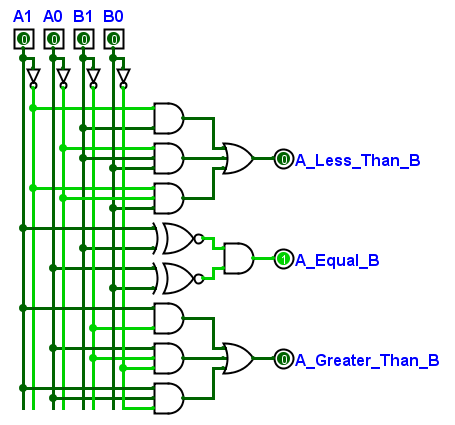
\includegraphics[width=\maxwidth{.95\linewidth}]{gfx/08_13}
	\caption{Two-Bit Comparator}
	\label{fig:08_13}
\end{figure}


\chapter{Combinational Encoder Circuits}\label{ch09}
\section{Introduction}

Electronic circuits that do not require any memory devices (like flip-flops or registers) use what is called ``Combinational Logic.'' These systems can be quite complex, but all outputs are determined solely by the actions of a series of logic gates on a given set of inputs. Another characteristic of combinational circuits is the lack of feedback. An output state is determined almost instantly from the inputs with no feedback loops. Combinational circuits can be reduced to a Boolean Algebra expression, though one that may be quite complex. Combinational circuits include many useful applications, including adders, subtractors, multipliers, dividers, encoders, decoders, display drivers, and keyboard encoders.
 
This chapter develops combinational logic circuits.\footnote{All circuits found in this chapter are available as \Le files in the course materials.}

\section{Multiplexers/Demultiplexers}
\label{CL:sec:multiplexers_demultiplexers}

\subsection{Multiplexer}
\label{CL:subsec:multiplexer}

\marginpar{A multiplexer is usually called a ``mux'' and a demultiplexer is called a ``dmux.''}

A multiplexer is used to connect one of several input lines to a single output line. Thus, it selects which input to pass to the output. This function is similar to a rotary switch where several potential inputs to the switch can be sent to a single output. A demultiplexer is a multiplexer in reverse, so a single input can be routed to any of several outputs. While mux/dmux circuits were originally built for transmission systems (like using a single copper wire to carry several different telephone calls simultaneously), today they are used as ``decision-makers'' in virtually every digital logic system and are, therefore, one of the most important devices for circuit designers. 

To help clarify this concept, Figure \ref{CL:fig:multiplexer_using_rotary_switches} is a simple schematic diagram that shows two rotary switches set up as a mux/dmux pair. As the switches are set in the diagram, a signal would travel from \textsf{INPUT B} to \textsf{OUTPUT 2} through a connecting wire. 

\begin{figure}[H]
  \caption{Multiplexer Using Rotary Switches}
  \label{CL:fig:multiplexer_using_rotary_switches}  
  \myfloatalign
  \begin{tikzpicture} [circuit logic US, scale=1.00]
  % make all path lines (the node shapes) a little thicker
  \tikzstyle{every path}=[line width=0.50mm]  
  
  % Input nodes
  \node[circ,label={135:A}] (nA) at (0.40,2.50) {};
  \node[circ,label={180:B}] (nB) at (0.15,2.35) {};
  \node[circ,label={180:C}] (nC) at (0.0,2.00) {};
  \node[circ,label={180:D}] (nD) at (0.15,1.65) {};
  \node[circ,label={225:E}] (nE) at (0.40,1.50) {};
  % Connector Nodes
  \node[circ] (c01) at (0.5,2.00) {};
  \node[circ] (c02) at (2.0,2.00) {};  
  % Output nodes
  \node[circ,label={45:1}] (o1)  at (2.1,2.50) {};
  \node[circ,label={0:2}]  (o2)  at (2.35,2.35) {};
  \node[circ,label={0:3}]  (o3)  at (2.5,2.00) {};
  \node[circ,label={0:4}]  (o4)  at (2.35,1.65) {};
  \node[circ,label={315:5}] (o5) at (2.1,1.50) {};
  
  % Draw the lines
  \pgfsetarrowsend{latex};
  \draw (c01) -- (nB);
  \draw (c02) -- (o2);

  \pgfsetarrowsend{};
  \draw (c02) -- (c01) ;    
  \end{tikzpicture}
\end{figure}

Imagine that the switches could somehow be synchronized so they rotated among the setting together; that is, \textsf{INPUT A}  would always connect to \textsf{OUTPUT 1} and so forth. That would mean a single wire could carry five different signals. For example, imagine that the inputs were connected to five different intrusion sensors in a building and the five outputs were connected to lamps on a guard's console in a remote building. If something triggered sensor $ A $ then as soon as the mux/dmux pair rotated to that position it would light lamp one on the console. Carrying all of these signals on a single wire saves a lot of expense. Of course, a true alarm system would be more complex than this, but this example is only designed to illustrate how a mux/dmux pair works in a transmission system.

\footnote{In this book, input data ports are labeled with a single letter from the beginning of the alphabet, output data ports are labeled with a single letter from the end of the alphabet, and other signals use descriptive labels.}Figure \ref{fig:08_01} is the logic diagram for a simple one-bit two-to-one multiplexer. In this circuit, an input is applied to input ports \emph{A} and \emph{B}. Port \emph{Sel} is the selector and if that signal is zero then Port \emph{A} will be routed to output \emph{Y}; if, though, \emph{Sel} is one then Port \emph{B} will be routed to \emph{Y}.

\begin{figure}[H]
	\centering
	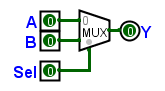
\includegraphics[width=\maxwidth{.95\linewidth}]{gfx/08_01}
	\caption{Simple Mux}
	\label{fig:08_01}
\end{figure}

Truth Table \ref{tab:08_01}, below, is for a multiplexer:

\begin{table}[H]
  \sffamily
  \newcommand{\head}[1]{\textcolor{white}{\textbf{#1}}}    
  \begin{center}
    \rowcolors{2}{gray!10}{white} % Color every other line a light gray
    \begin{tabular}{cc|cc} 
      \rowcolor{black!75}
      \multicolumn{3}{c}{\head{Inputs}} & \head{Output} \\
      A & B & Sel & Y \\
      \hline
      0 & 0 & 0 & 0 \\
      0 & 0 & 1 & 0 \\
      0 & 1 & 0 & 0 \\
      0 & 1 & 1 & 1 \\
      1 & 0 & 0 & 1 \\
      1 & 0 & 1 & 0 \\
      1 & 1 & 0 & 1 \\
      1 & 1 & 1 & 1 
    \end{tabular}
  \end{center}
  \caption{Truth Table for a Multiplexer}
  \label{tab:08_01}
\end{table}

In this multiplexer, the data input ports are only a single bit wide; however, in a normal circuit those ports could be a full $ 32 $-bit or $ 64 $-bit word and the selected word would be passed to the output port. Moreover, a multiplexer can have more than two input ports so a very versatile switch can be built to handle switching full words from one of eight or even sixteen different inputs. Because of its ability to channel a selected data stream to a single bus line from many different sub-circuits, the multiplexer is one of the workhorses for digital logic circuits and is frequently found in complex devices like \acp{CPU}.
 
\subsection{Demultiplexer}
\label{CL:subsec:demultiplexer}

A demultiplexer is the functional opposite of a multiplexer: a single input is routed to one of several potential outputs. Figure \ref{fig:08_02} is the logic diagram for a one-bit one-to-two demultiplexer. In this circuit, an input is applied to input port \emph{A}. Port \emph{Sel} is a control signal and if that signal is zero then input \emph{A} will be routed to output \emph{Y}, but if the control signal is one then input \emph{A} will be routed to output \emph{Z}.

\begin{figure}[H]
	\centering
	\includegraphics[width=\maxwidth{.95\linewidth}]{gfx/08_02}
	\caption{Simple Dmux}
	\label{fig:08_02}
\end{figure}

Truth Table \ref{tab:08_02}, below, is for a demultiplexer.

\begin{table}[H]
  \sffamily
  \newcommand{\head}[1]{\textcolor{white}{\textbf{#1}}}    
  \begin{center}
    \rowcolors{2}{gray!10}{white} % Color every other line a light gray
    \begin{tabular}{cc|cc} 
      \rowcolor{black!75}
      \multicolumn{2}{c}{\head{Inputs}} & \multicolumn{2}{c}{\head{Outputs}} \\
      A & Sel & Y & Z \\
      \hline
      0 & 0 & 0 & 0 \\
      0 & 1 & 0 & 0 \\
      1 & 0 & 0 & 1 \\
      1 & 1 & 1 & 0 
    \end{tabular}
  \end{center}
  \caption{Truth Table for a Demultiplexer}
  \label{tab:08_02}
\end{table}

In this demultiplexer the data input port is only a single bit wide; however, in a normal circuit that port could be a full $ 32 $-bit or $ 64 $-bit word and that entire word would be passed to the selected output port. Moreover, a demultiplexer can have more than two outputs so a very versatile switch can be built to handle switching full words to one of eight or even sixteen different outputs. Because of its ability to switch a data stream to different sub-circuits, the demultiplexer is one of the workhorses for digital logic circuits and is frequently found in complex devices like \acp{CPU}.

\subsection{Minterm Generators}
\label{CL:subsec:minterm_generators}

Demultiplexers can be combined with an \textsf{OR} gate and be used as a minterm generator. Consider the circuit for this two-variable equation.

\begin{align}
  \label{CL:eq:2_var_minterm_gen}
  \int(A,B) &= \sum(1,2)
\end{align}

Since there are two input variables, \emph{A} and \emph{B}, the dmux needs to have two select bits, one for each variable, and that would generate four potential dmux outputs \emph{W}, \emph{X}, \emph{Y}, and \emph{Z}. This circuit could be constructed using a four-output dmux with a two-bit control signal.

\begin{figure}[H]
	\centering
	\includegraphics[width=\maxwidth{.95\linewidth}]{gfx/08_03}
	\caption{1-to-4 Dmux}
	\label{fig:08_03}
\end{figure}

In Figure \ref{fig:08_03}, a four-bit input (\emph{A}) is routed to one of four output ports: \emph{W}, \emph{X}, \emph{Y}, or \emph{Z}, depending on the setting of the select, \emph{Sel}. Figure \ref{fig:08_03} shows the data input of $ 1010 $ being routed to \emph{Y} by a select of $ 10 $.

However, the equation specifies that the only outputs that would be used are when \emph{Sel} is $ 01 $ or $ 10 $. Thus, output ports \emph{X} and \emph{Y} must be sent to an \textsf{OR} gate and the other two outputs ignored. The output of the \textsf{OR} gate would only activate when \emph{Sel} is set to $ 01 $ or $ 10 $, as shown in Figure \ref{fig:08_04}. 

\begin{figure}[H]
	\centering
	\includegraphics[width=\maxwidth{.95\linewidth}]{gfx/08_04}
	\caption{1-to-4 Dmux As Minterm Generator}
	\label{fig:08_04}
\end{figure}


\section{Encoders/Decoders}
\label{CL:sec:encoders_decoders}

\subsection{Introduction}
\label{CL:subsec:introduction_to_encoders_decoders}

Encoders and decoders are used to convert some sort of coded data into a different code. For example, it may be necessary to convert the code created by a keyboard into \ac{ASCII} for use in a word processor. By definition, the difference between an encoder and a decoder is the number of inputs and outputs: Encoders have more inputs than outputs, while decoders have more outputs than inputs. 

As an introduction to encoders, consider Figure \ref{fig:08_14}, which is designed to encode three single line inputs (maybe three different push buttons on a control panel) into a binary number for further processing by the computer. In this circuit, the junction between the two \textsf{OR} gates and the output ($ Y $) is a \emph{joiner} that combines two bit streams into a single bus. Physically, two wires (one from \emph{U1} and one from \emph{U2}) would be spliced together into a single cable (a \emph{bus}) that contains two strands. The figure shows that when input \emph{C} is active the output of the encoder is $ 11 $.

\begin{figure}[H]
	\centering
	\includegraphics[width=\maxwidth{.95\linewidth}]{gfx/08_14}
	\caption{Three-line to 2-Bit Encoder}
	\label{fig:08_14}
\end{figure}
 
As an introduction to decoders, consider Figure \ref{fig:08_15}, which is designed to decode a two-bit binary input and drive a single output line high. A circuit like this may be used to light an \ac{LED} used as a warning on a console if a particular binary code is generated elsewhere in a circuit. In this circuit, the input is a two-bit number ($ 10 $ in the illustration), but those two bits are separated through a splitter and each is applied to one of the inputs of a series of four \textsf{AND} gates. Imagine that the \ac{MSB} was placed on the wire on the left of the grid and wired to the bottom input of each of the \textsf{AND} gates. If $ A=10 $, then \textsf{AND} gate three would activate and output \emph{X} would go high.

\begin{figure}[H]
	\centering
	\includegraphics[width=\maxwidth{.95\linewidth}]{gfx/08_15}
	\caption{Four-Bit to 4-Line Decoder}
	\label{fig:08_15}
\end{figure}

Both encoders and decoders are quite common and are used in many electronic devices. However, it is not very common to build these circuits out of discrete components (like in the circuits above). Rather, inexpensive integrated circuits are available for most encoder/decoder operations and these are much easier, and more reliable, to use. 

\subsection{Ten-Line Priority}
\label{CL:subsec:10_line_priority}

\marginpar{This encoder is sometimes called Ten-Line to Four-Line.}

Consider a ten-key keypad containing the numbers zero through nine, like a keypad that could be used for numeric input from some hand-held device. In order to be useful, a key press would need to be encoded to a binary number for further processing by a logic circuit. 

The keypad outputs a nine-bit number such that a single bit goes high to indicate which key was. For example, when key number two is pressed, $ 0\_0000\_0010 $ is output from the device. A priority encoder would accept that nine-bit number and output a binary number that could be used in computer circuits. Truth Table \ref{CL:tab:truth_table_for_priority_encoder} is for the Priority Encoder that meets the specification. The device is called a ``priority'' encoder since it will respond to only the highest value key press. For example, if someone pressed the three and five keys simultaneously the encoder would ignore the three key press and transmit $ 0101 $, or binary five.\marginpar{Dashes are normally used to indicate ``don't care'' on a Truth Table.}

\begin{table}[H]
  \sffamily
  \newcommand{\head}[1]{\textcolor{white}{\textbf{#1}}}    
  \begin{center}
    \rowcolors{2}{gray!10}{white} % Color every other line a light gray
    \begin{tabular}{ccccccccc|cccc} 
      \rowcolor{black!75}
      \multicolumn{9}{c}{\head{Inputs}} & \multicolumn{4}{c}{\head{Outputs}} \\
      9 & 8 & 7 & 6 & 5 & 4 & 3 & 2 & 1 & Y1 & Y2 & Y3 & Y4 \\
      \hline
      0 & 0 & 0 & 0 & 0 & 0 & 0 & 0 & 1 & 0 & 0 & 0 & 1 \\
      0 & 0 & 0 & 0 & 0 & 0 & 0 & 1 & - & 0 & 0 & 1 & 0 \\
      0 & 0 & 0 & 0 & 0 & 0 & 1 & - & - & 0 & 0 & 1 & 1 \\
      0 & 0 & 0 & 0 & 0 & 1 & - & - & - & 0 & 1 & 0 & 0 \\
      0 & 0 & 0 & 0 & 1 & - & - & - & - & 0 & 1 & 0 & 1 \\
      0 & 0 & 0 & 1 & - & - & - & - & - & 0 & 1 & 1 & 0 \\
      0 & 0 & 1 & - & - & - & - & - & - & 0 & 1 & 1 & 1 \\
      0 & 1 & - & - & - & - & - & - & - & 1 & 0 & 0 & 0 \\
      1 & - & - & - & - & - & - & - & - & 1 & 0 & 0 & 1
    \end{tabular}
  \end{center}
  \caption{Truth Table for Priority Encoder}
  \label{CL:tab:truth_table_for_priority_encoder}
\end{table}

This circuit can be realized by using a grid input and routing the various lines to an appropriate \emph{AND} gate. This is one of the circuits built in the lab manual that accompanies this text.

\subsection{Seven-Segment Display}
\label{CL:subsec:7_segment_display}

A seven-segment display is commonly used in calculators and other devices to show hexadecimal numbers. To create the numeric shapes, various segments are activated while others remain off, so binary numbers must be decoded to turn on the various segments for any given combination of inputs. A seven-segment display has eight input ports and, when high, each of those ports will activate one segment of the display. 

\begin{figure}[H]
  \caption{Seven-Segment Display}
  \label{CL:fig:seven_segment_display}  
  \myfloatalign
  \begin{tikzpicture} [circuit logic US, scale=1.00]
    \SSGLeg[3em]{};
    \SSGNb[3em]{}{2};
  \end{tikzpicture}
\end{figure}
 
\marginpar{Usually an eighth ``segment'' is available \textemdash a decimal point in the lower right corner.}

In Figure \ref{CL:fig:seven_segment_display} the seven segments are labeled and it shows that the number ``$ 2 $'' for example, is made by activating segments \textsf{a}, \textsf{b}, \textsf{g}, \textsf{e}, and \textsf{d}. Table \ref{CL:tab:truth_table_for_seven_segment_display} shows the various segments that must be activated for each of the $ 16 $ possible input values.

\begin{table}[H]
  \sffamily
  \newcommand{\head}[1]{\textcolor{white}{\textbf{#1}}}    
  \begin{center}
    \rowcolors{2}{gray!10}{white} % Color every other line a light gray
    \begin{tabular}{cccccccccccccc} 
      \rowcolor{black!75}
      \head{Hex} & \head{|} & \multicolumn{4}{c}{\head{Binary}} & \head{|} & \multicolumn{7}{c}{\head{Display}} \\
        &|& \textbf{3} & \textbf{2} & \textbf{1} & \textbf{0} &|& \textbf{a} & \textbf{b} & \textbf{c} & \textbf{d} & \textbf{e} & \textbf{f} & \textbf{g} \\
%      0 &|& 0 & 0 & 0 & 0 &|& a & b & c & d & e & f & g \\
      0 &|& 0 & 0 & 0 & 0 &|& 1 & 1 & 1 & 1 & 1 & 1 & 0 \\
      1 &|& 0 & 0 & 0 & 1 &|& 0 & 1 & 1 & 0 & 0 & 0 & 0 \\
      \textbf{2} &|& \textbf{0} & \textbf{0} & \textbf{1} & 
        \textbf{0} &|& \textbf{1} & \textbf{1} & \textbf{0} & 
        \textbf{1} & \textbf{1} & \textbf{0} & \textbf{1} \\
      3 &|& 0 & 0 & 1 & 1 &|& 1 & 1 & 1 & 1 & 0 & 0 & 1 \\
      4 &|& 0 & 1 & 0 & 0 &|& 0 & 1 & 1 & 0 & 0 & 1 & 1 \\
      5 &|& 0 & 1 & 0 & 1 &|& 1 & 0 & 1 & 1 & 0 & 1 & 1 \\
      6 &|& 0 & 1 & 1 & 0 &|& 1 & 0 & 1 & 1 & 1 & 1 & 1 \\
      7 &|& 0 & 1 & 1 & 1 &|& 1 & 1 & 1 & 0 & 0 & 0 & 0 \\
      8 &|& 1 & 0 & 0 & 0 &|& 1 & 1 & 1 & 1 & 1 & 1 & 1 \\
      9 &|& 1 & 0 & 0 & 1 &|& 1 & 1 & 1 & 1 & 0 & 1 & 1 \\
      A &|& 1 & 0 & 1 & 0 &|& 1 & 1 & 1 & 0 & 1 & 1 & 1 \\
      B &|& 1 & 0 & 1 & 1 &|& 0 & 0 & 1 & 1 & 1 & 1 & 1 \\
      C &|& 1 & 1 & 0 & 0 &|& 1 & 0 & 0 & 1 & 1 & 1 & 0 \\
      D &|& 1 & 1 & 0 & 1 &|& 0 & 1 & 1 & 1 & 1 & 0 & 1 \\
      E &|& 1 & 1 & 1 & 0 &|& 1 & 0 & 0 & 1 & 1 & 1 & 1 \\
      F &|& 1 & 1 & 1 & 1 &|& 1 & 0 & 0 & 0 & 1 & 1 & 1 
    \end{tabular}
  \end{center}
  \caption{Truth Table for Seven-Segment Display}
  \label{CL:tab:truth_table_for_seven_segment_display}
\end{table}

Notice that to display the number ``$ 2 $'' (in bold font), segments \textsf{a}, \textsf{b}, \textsf{d}, \textsf{e}, and \textsf{g} must be activated. 

A decoder circuit, as in Figure \ref{fig:08_16}, uses a demultiplexer to activate a one-bit line based on the value of the binary input. Note: to save space, two parallel decoders are used in this circuit.

\begin{figure}[H]
	\centering
	\includegraphics[width=\maxwidth{.95\linewidth}]{gfx/08_16}
	\caption{7-Segment Decoder}
	\label{fig:08_16}
\end{figure}

Figure \ref{fig:08_16} shows an input of $ 1111_2 $ so the last line on each demultiplexer is activated. Those lines are used to activate the necessary inputs on the seven-segment display to create an output of ``F''. 

A Hex Digit Display has a single port that accepts a four-bit binary number and that number is decoded into a digital display. Figure \ref{fig:08_17} shows a hex digit display. 

\begin{figure}[H]
	\centering
	\includegraphics[width=\maxwidth{.95\linewidth}]{gfx/08_17}
	\caption{Hex Decoder}
	\label{fig:08_17}
\end{figure}

The \Le simulator used in this class includes both a \emph{7-Segment Display} and a \emph{Hex Digit Display}. One of the strengths of using a seven-segment display rather than a hex digit display is that the circuit designer has total control over which segments are displayed. It is common, for example, to activate each of the outer segments in a rapid sequence to give the illusion of a rotating circle. As opposed to a seven-segment display, a hex digit display is very simple to wire and use, as Figures \ref{fig:08_16} and \ref{fig:08_17} make clear. Both of these two types of displays are available on the market and a designer would chose whichever type meets the needs. 

\subsection{Function Generators}
\label{CL:subsec:function_generators}

Decoders provide an easy way to create a circuit when given a minterm function. Imagine that a circuit is needed for the function defined in Equation \ref{CL:eq:decoder_as_minterm_gen}.

\begin{align}
  \label{CL:eq:decoder_as_minterm_gen}
  \int(A,B,C) &= \sum(0,2,7)
\end{align}

Whatever this circuit is designed to do, it should activate an output only when the input is zero, two, or seven. The circuit in Figure \ref{fig:08_18} illustrates a simple minterm generator using a demultiplexer and an \textsf{OR} gate. When input \emph{A} is zero, two, or seven then output \emph{Y} will go high, otherwise it is low.

\begin{figure}[H]
	\centering
	\includegraphics[width=\maxwidth{.95\linewidth}]{gfx/08_18}
	\caption{Minterm Generator}
	\label{fig:08_18}
\end{figure}

\section{Error Detection}
\label{CL:sec:error_detection}

\subsection{Introduction}
\label{CL:subsec:introduction_to_error_detection}

Whenever a byte (or any other group of bits) is transmitted or stored, there is always the possibility that one or more bits will be accidentally complemented. Consider these two binary numbers:

\begin{verbatim}
     0110 1010 0011 1010
     0110 1010 0111 1010
\end{verbatim} 

They differ by only one bit (notice Group Three). If the top number is what is supposed to be in a memory location but the bottom number is what is actually there then this would, obviously, create a problem. There could be any number of reasons why a bit would be wrong, but the most common is some sort of error that creeps in while the byte is being transmitted between two stores, like between a \ac{USB} drive and memory or between two computers sharing a network. It is desirable to be able to detect that a byte contains a bad bit and, ideally, even know which bit is wrong so it can be corrected. 

Parity is a common method used to check data for errors and it can be used to check data that has been transmitted, held in memory, or stored on a hard drive. The concept of parity is fairly simple: A bit (called the \emph{parity bit}) is added to each data byte and that extra bit is either set to zero or one in order to make the bit-count of that byte contain an even or odd number of ones. For example, consider this binary number: 

\begin{verbatim}
     1101
\end{verbatim}

There are three ones in this number, which is an odd number. If odd parity is being used in this circuit, then the parity bit would be zero so there would be an odd number of ones in the number. However, if the circuit is using even parity, then the parity bit would be set to one in order to have four ones in the number, which is an even number. Following is the above number with both even and odd parity bits (those parity bits are in the least significant position and are separated from the original number by a space for clarity): 

\begin{verbatim}
     1101 0 (Odd Parity)
     1101 1 (Even Parity)
\end{verbatim}

Table \ref{CL:tab:even_parity_examples} shows several examples that may help to clarify this concept. In each case, a parity bit is used to make the data byte even parity (spaces were left in the data byte for clarity). 

\begin{table}[H]
  \sffamily
  \newcommand{\head}[1]{\textcolor{white}{\textbf{#1}}}    
  \begin{center}
    \rowcolors{2}{gray!10}{white} % Color every other line a light gray
    \begin{tabular}{cc} 
      \rowcolor{black!75}
      \head{Data Byte} & \head{Parity Bit} \\
      0000 0000 & 0 \\
      0000 0001 & 1 \\
      0000 0011 & 0 \\
      0000 0100 & 1 \\
      1111 1110 & 1 \\
      1111 1111 & 0
    \end{tabular}
  \end{center}
  \caption{Even Parity Examples}
  \label{CL:tab:even_parity_examples}
\end{table}

Generating a parity bit can be done with a series of cascading \emph{XOR} gates but \Le had two parity gates, one that outputs high when the inputs have an odd number of ones and the other when there are an even number of ones. Figure \ref{fig:08_19} illustrates using an odd parity gate (labeled ``2K+1''). In this circuit, if input \emph{A} has an odd number of ones, as illustrated, then the parity generator will output a one to indicate input \emph{A} has an odd number of ones. That parity bit is added as the most significant bit to output \emph{Y}. Since output \emph{Y} will always have an even number of bits this is an even parity circuit.

\begin{figure}[H]
	\centering
	\includegraphics[width=\maxwidth{.95\linewidth}]{gfx/08_19}
	\caption{Parity Generator}
	\label{fig:08_19}
\end{figure}

Parity is a simple concept and is the foundation for one of the most basic methods of error checking. As an example, if some byte is transmitted using even parity but the data arrives with an odd number of ones then one of the bits was changed during transmission. 

\subsection{Iterative Parity Checking}
\label{CL:subsec:iterative_parity_checking}

One of the problems with using parity for error detection is that while it may be known that \emph{something} is wrong, there is no way to know which of the bits is wrong. For example, imagine an eight-bit system is using even parity and receives this data and parity bit:

\begin{verbatim}
     1001 1110 PARITY: 0
\end{verbatim} 

There is something wrong with the byte. It is indicating even parity but has an odd number of ones in the byte. It is impossible to know which bit changed during transmission. In fact, it may be that the byte is correct but the parity bit itself changed (a \emph{false error}). It would be nice if the parity error detector would not only indicate that there was an error, but could also determine which bit changed so it could be corrected. 

One method of error correction is what is known as \emph{Iterative Parity Checking}. Imagine that a series of eight-bit bytes were being transmitted. Each byte would have a parity bit attached; however, there would also be a parity byte that contains a parity bit for each bit in the preceding five bytes. It is easiest to understand this by using a table (even parity is being used):

\begin{table}[H]
  \sffamily
  \newcommand{\head}[1]{\textcolor{white}{\textbf{#1}}}    
  \begin{center}
    \rowcolors{2}{gray!10}{white} % Color every other line a light gray
    \begin{tabular}{cccccccccc} 
      \rowcolor{black!75}
      \head{Byte} & \multicolumn{8}{c}{\head{Data}} & \head{Parity} \\
      1 & 0 & 0 & 0 & 0 & 0 & 0 & 0 & 0 & 0 \\
      2 & 1 & 0 & 1 & 1 & 0 & 0 & 0 & 0 & 1 \\
      3 & 1 & 0 & 1 & 1 & 0 & 0 & 1 & 1 & 1 \\
      4 & 1 & 1 & 1 & 0 & 1 & 0 & 1 & 0 & 1 \\
      5 & 0 & 1 & 0 & 0 & 0 & 0 & 0 & 0 & 1 \\
      P & 1 & 0 & 1 & 0 & 1 & 0 & 0 & 1 & 0
    \end{tabular}
  \end{center}
  \caption{Iterative Parity}
  \label{CL:tab:iterative_parity}
\end{table}
 
In Table \ref{CL:tab:iterative_parity}, Byte one is $ 0000\;0000 $. Since the system is set for even parity, and it is assumed that a byte with all zeros is even, then the parity bit is zero. Each of the five bytes has a parity bit that is properly set such that each byte (with the parity bit) includes an even number of bits. Then, after a group of five bytes a \emph{parity byte} is inserted into the data stream so that each column of five bits also has a parity check; and that parity bit is found in row $ P $ on the table. Thus, the parity bit at the bottom of the first column is one since that column has three other ones. As a final check, the parity byte itself also has a parity bit added. 

Table \ref{CL:tab:iterative_parity_with_error} is the same as Table \ref{CL:tab:iterative_parity}, but Bit Zero, the least significant bit, in Byte One has been changed from a zero to a one (that number is highlighted).

\begin{table}[H]
  \sffamily
  \newcommand{\head}[1]{\textcolor{white}{\textbf{#1}}}    
  \begin{center}
    \rowcolors{2}{gray!10}{white} % Color every other line a light gray
    \begin{tabular}{cccccccccc} 
      \rowcolor{black!75}
      \head{Byte} & \multicolumn{8}{c}{\head{Data}} & \head{Parity} \\
      1 & 0 & 0 & 0 & 0 & 0 & 0 & 0 & \cellcolor{yellow!70!white}1 & 0 \\
      2 & 1 & 0 & 1 & 1 & 0 & 0 & 0 & 0 & 1 \\
      3 & 1 & 0 & 1 & 1 & 0 & 0 & 1 & 1 & 1 \\
      4 & 1 & 1 & 1 & 0 & 1 & 0 & 1 & 0 & 1 \\
      5 & 0 & 1 & 0 & 0 & 0 & 0 & 0 & 0 & 1 \\
      P & 1 & 0 & 1 & 0 & 1 & 0 & 0 & 1 & 0
    \end{tabular}
  \end{center}
  \caption{Iterative Parity With Error}
  \label{CL:tab:iterative_parity_with_error}
\end{table}

In Table \ref{CL:tab:iterative_parity_with_error} the parity for Byte One is wrong, and the parity for Bit Zero in the parity byte is wrong; therefore, Bit Zero in Byte One needs to be changed. If the parity bit for a row is wrong, but no column parity bits are wrong, or a column is wrong but no rows are wrong, then the parity bit itself is incorrect. This is one simple way to not only detect data errors, but correct those errors. 

There are two weaknesses with iterative parity checking. First, it is restricted to only single-bit errors. If more than one bit is changed in a group then the system fails. This, though, is a general weakness for most parity checking schemes. The second weakness is that a parity byte must be generated and transmitted for every few data bytes (five in the example). This increases the transmission time dramatically and normally makes the system unacceptably slow.

\subsection{Hamming Code}
\label{CL:subsec:hamming_code}

\subsubsection{Introduction}
\label{CL:subsubsec:introduction_to_hamming_code}

Richard Hamming worked at Bell labs in the $ 1940 $s and he devised a way to not only detect that a transmitted byte had changed, but exactly which bit had changed by interspersing parity bits within the data itself. Hamming first defined the ``distance'' between any two binary words as the number of bits that were different between them. As an example, the two binary numbers $ 1010 $ and $ 1010 $ has a distance of zero between them since there are no different bits, but $ 1010 $ and $ 1011 $ has a distance of one since one bit is different. This concept is called the \emph{Hamming Distance} in honor of his work.

The circuit illustrated in Figure \ref{fig:08_20} calculates the Hamming distance between two four-bit numbers. In the illustration, $ 0100 $ and $ 1101 $ are compared and two bits difference in those two numbers is reported.

\begin{figure}[H]
	\centering
	\includegraphics[width=\maxwidth{.95\linewidth}]{gfx/08_20}
	\caption{Hamming Distance}
	\label{fig:08_20}
\end{figure}

The four bits for input \emph{A} and input \emph{B} are wired to four \textsf{XOR} gates then the output of those gates is wired to a \emph{Bit Adder} device. The \textsf{XOR} gates will output a one if the two input bits are different then the bit adder will total how many ones are present at its input. The output of the bit adder is a three-bit number but to make it easier to read that number it is wired to a hex digit display. Since that display needs a four-bit input a constant zero is wired to the most significant bit of the input of the hex digit display.

\subsubsection{Generating Hamming Code}
\label{CL:subsubsec:generating_hamming_code}

Hamming parity is designed so a parity bit is generated for various combinations of bits within a byte in such a way that every data bit is linked to at least three different parity bits. This system can then determine not only that the parity is wrong but which bit is wrong. The cost of a Hamming system is that it adds five parity bits to an eight-bit byte to create a $ 13 $-bit word. Consider the bits for the $ 13 $-bit word in Table \ref{cl:tab:hamming_parity_bits}.

\begin{table}[H]
  \sffamily
  \newcommand{\head}[1]{\textcolor{white}{\textbf{#1}}}		
  \begin{center}
    \rowcolors{2}{gray!10}{white} % Color every other line a light gray
    \begin{tabular}{ccccccccccccc} 
      \rowcolor{black!75}
      \head{$ P_4 $} & \head{$ d_7 $} & \head{$ d_6 $} &
      \head{$ d_5 $} & \head{$ d_4 $} & \head{$ P_3 $} &
      \head{$ d_3 $} & \head{$ d_2 $} & \head{$ d_1 $} &
      \head{$ P_2 $} & \head{$ d_0 $} & \head{$ P_1 $} &
      \head{$ P_0 $} \\
      $ 0 $ & $ 0 $ & $ 0 $ &
      $ 0 $ & $ 0 $ & $ 0 $ &
      $ 0 $ & $ 0 $ & $ 0 $ &
      $ 0 $ & $ 0 $ & $ 0 $ &
      $ 0 $ 
    \end{tabular}
  \end{center}
  \caption{Hamming Parity Bits}
  \label{cl:tab:hamming_parity_bits}
\end{table}

The bits numbered $ P_0 $ to $ P_4 $ are Hamming parity bits and the bits numbered $ d_0 $ to $ d_7 $ are the data bits. The Hamming parity bits are interspersed with the data but they occur in positions zero, one, three, and seven (counting right to left). The following chart shows the data bits that are used to create each parity bit: 

\begin{table}[H]
  \sffamily
  \newcommand{\head}[1]{\textcolor{white}{\textbf{#1}}}		
  \begin{center}
    \rowcolors{2}{gray!10}{white} % Color every other line a light gray
    \begin{tabular}{ccccccccccccc} 
      \rowcolor{black!75}
      \head{$ P_4 $} & \head{$ d_7 $} & \head{$ d_6 $} &
      \head{$ d_5 $} & \head{$ d_4 $} & \head{$ P_3 $} &
      \head{$ d_3 $} & \head{$ d_2 $} & \head{$ d_1 $} &
      \head{$ P_2 $} & \head{$ d_0 $} & \head{$ P_1 $} &
      \head{$ P_0 $} \\
      % Line P0
      \color{gray}{$ 0 $} & \color{gray}{$ 0 $} & $ X $ &
      \color{gray}{$ 0 $} & $ X $ & \color{gray}{$ 0 $} &
      $ X $ & \color{gray}{$ 0 $} & $ X $ &
      \color{gray}{$ 0 $} & $ X $ & \color{gray}{$ 0 $} &
      \color{red}{$ P $} \\
      % Line P1
      \color{gray}{$ 0 $} & \color{gray}{$ 0 $} & $ X $ &
      $ X $ & \color{gray}{$ 0 $} & \color{gray}{$ 0 $} &
      $ X $ & $ X $ & \color{gray}{$ 0 $} &
      \color{gray}{$ 0 $} & $ X $ & \color{red}{$ P $} &
      \color{gray}{$ 0 $} \\
      % Line P2
      \color{gray}{$ 0 $} & $ X $ & \color{gray}{$ 0 $} &
      \color{gray}{$ 0 $} & \color{gray}{$ 0 $} & \color{gray}{$ 0 $} &
      $ X $ & $ X $ & $ X $ &
      \color{red}{$ P $} & \color{gray}{$ 0 $} & \color{gray}{$ 0 $} &
      \color{gray}{$ 0 $} \\
      % Line P3
      \color{gray}{$ 0 $} & $ X $ & $ X $ &
      $ X $ & $ X $ & \color{red}{$ P $} &
      \color{gray}{$ 0 $} & \color{gray}{$ 0 $} & \color{gray}{$ 0 $} &
      \color{gray}{$ 0 $} & \color{gray}{$ 0 $} & \color{gray}{$ 0 $} &
      \color{gray}{$ 0 $} \\
      % Line P4
      \color{red}{$ P $} & $ X $ & \color{gray}{$ 0 $} &
      $ X $ & $ X $ & \color{gray}{$ 0 $} &
      \color{gray}{$ 0 $} & $ X $ & $ X $ &
      \color{gray}{$ 0 $} & $ X $ & \color{gray}{$ 0 $} &
      \color{gray}{$ 0 $} 
    \end{tabular}
  \end{center}
  \caption{Hamming Parity Cover Table}
  \label{cl:tab:hamming_parity_cover_table}
\end{table}

From Table \ref{cl:tab:hamming_parity_cover_table}, line one shows the data bits that are used to set parity bit zero ($ P_{0} $). If data bits $ d0 $, $ d1 $, $ d3 $, $ d4 $, and $ d6 $ are all one then $ P_{0} $ would be one (even parity is assumed). The data bits needed to create the Hamming parity bit are marked in all five lines. A note is necessary about parity bit $ P_4 $. In order to detect transmission errors that are two bits large (that is, two bits were flipped), each data bit needs to be covered by three parity bits. Parity bit $ P_4 $ is designed to provide the third parity bit for any data bits that have only two others. For example, look down the column containing data bit $ d_0 $ and notice that it has only two parity bits ($ P_0 $ and $ P_1 $) before $ P_4 $. By adding $ P_4 $ to the circuit that data bit gets a third parity bit.

As an example of a Hamming code, imagine that this byte needed to be transmitted: $ 0110 \; 1001 $. This number could be placed in the data bit positions of the Hamming table. 

\begin{table}[H]
  \sffamily
  \newcommand{\head}[1]{\textcolor{white}{\textbf{#1}}}		
  \begin{center}
    \rowcolors{2}{gray!10}{white} % Color every other line a light gray
    \begin{tabular}{ccccccccccccc} 
      \rowcolor{black!75}
      \head{$ P_4 $} & \head{$ d_7 $} & \head{$ d_6 $} &
      \head{$ d_5 $} & \head{$ d_4 $} & \head{$ P_3 $} &
      \head{$ d_3 $} & \head{$ d_2 $} & \head{$ d_1 $} &
      \head{$ P_2 $} & \head{$ d_0 $} & \head{$ P_1 $} &
      \head{$ P_0 $} \\
      \color{gray}{$ 0 $} & $ 0 $ & $ 1 $ &
      $ 1 $ & $ 0 $ & \color{gray}{$ 0 $} &
      $ 1 $ & $ 0 $ & $ 0 $ &
      \color{gray}{$ 0 $} & $ 1 $ & \color{gray}{$ 0 $} &
      \color{gray}{$ 0 $}
    \end{tabular}
  \end{center}
  \caption{Hamming Example - Iteration 1}
  \label{cl:tab:hamming_example_iteration_1}
\end{table}

Bit zero, $ P0 $, is designed to generate even parity for data bits $ d_0 $, $ d_1 $, $ d_3 $, $ d_4 $, and $ d_6 $. Since there are three ones in that group, then $ P_0 $ must be one. That has been filled in below (for convenience, the Hamming parity bit pattern for $ P_0 $ is included in the last row of the table). 

\begin{table}[H]
  \sffamily
  \newcommand{\head}[1]{\textcolor{white}{\textbf{#1}}}		
  \begin{center}
    \rowcolors{2}{gray!10}{white} % Color every other line a light gray
    \begin{tabular}{ccccccccccccc} 
      \rowcolor{black!75}
      \head{$ P_4 $} & \head{$ d_7 $} & \head{$ d_6 $} &
      \head{$ d_5 $} & \head{$ d_4 $} & \head{$ P_3 $} &
      \head{$ d_3 $} & \head{$ d_2 $} & \head{$ d_1 $} &
      \head{$ P_2 $} & \head{$ d_0 $} & \head{$ P_1 $} &
      \head{$ P_0 $} \\
      \color{gray}{$ 0 $} & $ 0 $ & $ 1 $ &
      $ 1 $ & $ 0 $ & \color{gray}{$ 0 $} &
      $ 1 $ & $ 0 $ & $ 0 $ &
      \color{gray}{$ 0 $} & $ 1 $ & \color{gray}{$ 0 $} &
      \color{red}{$ 1 $} \\
      % Line P0
      \color{gray}{$ 0 $} & \color{gray}{$ 0 $} & $ X $ &
      \color{gray}{$ 0 $} & $ X $ & \color{gray}{$ 0 $} &
      $ X $ & \color{gray}{$ 0 $} & $ X $ &
      \color{gray}{$ 0 $} & $ X $ & \color{gray}{$ 0 $} &
      \color{red}{$ P $} \\      
    \end{tabular}
  \end{center}
  \caption{Hamming Example - Iteration 2}
  \label{cl:tab:hamming_example_iteration_2}
\end{table}

Bit one, $ P_1 $, is designed to generate even parity for data bits $ d_0 $, $ d_2 $, $ d_3 $, $ d_5 $, and $ d_6 $. Since there are four ones in that group, then $ P_1 $ must be zero. That has been filled in below. 

\begin{table}[H]
  \sffamily
  \newcommand{\head}[1]{\textcolor{white}{\textbf{#1}}}		
  \begin{center}
    \rowcolors{2}{gray!10}{white} % Color every other line a light gray
    \begin{tabular}{ccccccccccccc} 
      \rowcolor{black!75}
      \head{$ P_4 $} & \head{$ d_7 $} & \head{$ d_6 $} &
      \head{$ d_5 $} & \head{$ d_4 $} & \head{$ P_3 $} &
      \head{$ d_3 $} & \head{$ d_2 $} & \head{$ d_1 $} &
      \head{$ P_2 $} & \head{$ d_0 $} & \head{$ P_1 $} &
      \head{$ P_0 $} \\
      \color{gray}{$ 0 $} & $ 0 $ & $ 1 $ &
      $ 1 $ & $ 0 $ & \color{gray}{$ 0 $} &
      $ 1 $ & $ 0 $ & $ 0 $ &
      \color{gray}{$ 0 $} & $ 1 $ & \color{red}{$ 0 $} &
      $ 1 $ \\
      % Line P1
      \color{gray}{$ 0 $} & \color{gray}{$ 0 $} & $ X $ &
      $ X $ & \color{gray}{$ 0 $} & \color{gray}{$ 0 $} &
      $ X $ & $ X $ & \color{gray}{$ 0 $} &
      \color{gray}{$ 0 $} & $ X $ & \color{red}{$ P $} &
      \color{gray}{$ 0 $} \\
    \end{tabular}
  \end{center}
  \caption{Hamming Example - Iteration 3}
  \label{cl:tab:hamming_example_iteration_3}
\end{table}

Bit three, $ P_2 $, is designed to generate even parity for data bits $ d_1 $, $ d_2 $, $ d_3 $, and $ d_7 $. Since there is one one in that group, then $ P_2 $ must be one. That has been filled in below. 

\begin{table}[H]
  \sffamily
  \newcommand{\head}[1]{\textcolor{white}{\textbf{#1}}}		
  \begin{center}
    \rowcolors{2}{gray!10}{white} % Color every other line a light gray
    \begin{tabular}{ccccccccccccc} 
      \rowcolor{black!75}
      \head{$ P_4 $} & \head{$ d_7 $} & \head{$ d_6 $} &
      \head{$ d_5 $} & \head{$ d_4 $} & \head{$ P_3 $} &
      \head{$ d_3 $} & \head{$ d_2 $} & \head{$ d_1 $} &
      \head{$ P_2 $} & \head{$ d_0 $} & \head{$ P_1 $} &
      \head{$ P_0 $} \\
      \color{gray}{$ 0 $} & $ 0 $ & $ 1 $ &
      $ 1 $ & $ 0 $ & \color{gray}{$ 0 $} &
      $ 1 $ & $ 0 $ & $ 0 $ &
      \color{red}{$ 1 $} & $ 1 $ & $ 0 $ &
      $ 1 $ \\
      % Line P2
      \color{gray}{$ 0 $} & $ X $ & \color{gray}{$ 0 $} &
      \color{gray}{$ 0 $} & \color{gray}{$ 0 $} & \color{gray}{$ 0 $} &
      $ X $ & $ X $ & $ X $ &
      \color{red}{$ P $} & \color{gray}{$ 0 $} & \color{gray}{$ 0 $} &
      \color{gray}{$ 0 $} \\
    \end{tabular}
  \end{center}
  \caption{Hamming Example - Iteration 4}
  \label{cl:tab:hamming_example_iteration_4}
\end{table}

Bit seven, $ P_3 $, is designed to generate even parity for data bits $ d_4 $, $ d_5 $, $ d_6 $, and $ d_7 $. Since there are two ones in that group, then $ P_3 $ must be zero. That has been filled in below. 

\begin{table}[H]
  \sffamily
  \newcommand{\head}[1]{\textcolor{white}{\textbf{#1}}}		
  \begin{center}
    \rowcolors{2}{gray!10}{white} % Color every other line a light gray
    \begin{tabular}{ccccccccccccc} 
      \rowcolor{black!75}
      \head{$ P_4 $} & \head{$ d_7 $} & \head{$ d_6 $} &
      \head{$ d_5 $} & \head{$ d_4 $} & \head{$ P_3 $} &
      \head{$ d_3 $} & \head{$ d_2 $} & \head{$ d_1 $} &
      \head{$ P_2 $} & \head{$ d_0 $} & \head{$ P_1 $} &
      \head{$ P_0 $} \\
      \color{gray}{$ 0 $} & $ 0 $ & $ 1 $ &
      $ 1 $ & $ 0 $ & \color{red}{$ 0 $} &
      $ 1 $ & $ 0 $ & $ 0 $ &
      $ 1 $ & $ 1 $ & $ 0 $ &
      $ 1 $ \\
      % Line P3
      \color{gray}{$ 0 $} & $ X $ & $ X $ &
      $ X $ & $ X $ & \color{red}{$ P $} &
      \color{gray}{$ 0 $} & \color{gray}{$ 0 $} & \color{gray}{$ 0 $} &
      \color{gray}{$ 0 $} & \color{gray}{$ 0 $} & \color{gray}{$ 0 $} &
      \color{gray}{$ 0 $} \\
    \end{tabular}
  \end{center}
  \caption{Hamming Example - Iteration 5}
  \label{cl:tab:hamming_example_iteration_5}
\end{table}

Bit eight, $ P_4 $, is designed to generate even parity for data bits $ d_0 $, $ d_1 $, $ d_2 $, $ d_4 $, $ d_5 $, and $ d_7 $. Since there are two ones in that group, then $ P_4 $ must be zero. That has been filled in below. 

\begin{table}[H]
  \sffamily
  \newcommand{\head}[1]{\textcolor{white}{\textbf{#1}}}		
  \begin{center}
    \rowcolors{2}{gray!10}{white} % Color every other line a light gray
    \begin{tabular}{ccccccccccccc} 
      \rowcolor{black!75}
      \head{$ P_4 $} & \head{$ d_7 $} & \head{$ d_6 $} &
      \head{$ d_5 $} & \head{$ d_4 $} & \head{$ P_3 $} &
      \head{$ d_3 $} & \head{$ d_2 $} & \head{$ d_1 $} &
      \head{$ P_2 $} & \head{$ d_0 $} & \head{$ P_1 $} &
      \head{$ P_0 $} \\
      \color{red}{$ 0 $} & $ 0 $ & $ 1 $ &
      $ 1 $ & $ 0 $ & $ 0 $ &
      $ 1 $ & $ 0 $ & $ 0 $ &
      $ 1 $ & $ 1 $ & $ 0 $ &
      $ 1 $ \\
      % Line P4
      \color{red}{$ P $} & $ X $ & \color{gray}{$ 0 $} &
      $ X $ & $ X $ & \color{gray}{$ 0 $} &
      \color{gray}{$ 0 $} & $ X $ & $ X $ &
      \color{gray}{$ 0 $} & $ X $ & \color{gray}{$ 0 $} &
      \color{gray}{$ 0 $} 
    \end{tabular}
  \end{center}
  \caption{Hamming Example - Iteration 6}
  \label{cl:tab:hamming_example_iteration_6}
\end{table}

When including Hamming parity, the byte $ 0110 \; 1001 $ is converted to: $ 0 \; 0110 \; 0100 \; 1101 $.

In Figure \ref{fig:08_21}, a 11-bit input, \emph{A}, is used to create a 16-bit word that includes Hamming parity bits. In the illustration, input $ 010 \; 0111 \; 0111 $ is converted to $ 1010 \; 0100 \; 1110 \; 1111 $.  

\begin{figure}[H]
	\centering
	\includegraphics[width=\maxwidth{.95\linewidth}]{gfx/08_21}
	\caption{Generating Hamming Parity}
	\label{fig:08_21}
\end{figure}

The process used by the circuit in Figure \ref{fig:08_21} is to wire each of the input bits to various parity generators and then combine the outputs of those parity generators, along with the original bits, into a single 16-bit word. While the circuit has a lot of wired connections the concept is fairly simple. \textsf{P0} calculates the parity for input bits $ 0, 1, 3, 4, 6, 8, 10 $. That is then wired to the least significant bit of output \emph{Y}.

\subsubsection{Checking Hamming Code}
\label{CL:subsubsec:checking_hamming_code}

To check the accuracy of the data bits in a word that contains Hamming parity bits the following general process is used:

\begin{enumerate}
  \item Calculate the Hamming Parity Bit for each of the bit groups exactly like when the parity was first calculated.
  \item Compare the calculated Hamming Parity bits with the parity bits found in the original binary word.
  \item If the parity bits match then there is no error. If the parity bits do not match then the bad bit can be corrected by using the pattern of parity bits that do not match.
\end{enumerate}

As an example, imagine that bit eight (last bit in the first group of four) in the Hamming code created above was changed from zero to one: $ 0 \; 011\underline{1} \; 0100 \; 1101 $ (this is bit $ d_4 $).  Table \ref{cl:tab:hamming_parity_cover_table_reproduced} shows that Hamming Bits $ P_0 $, $ P_3 $, and $ P_4 $ would now be incorrect since $ d_4 $ is used to create those parity bits.

\begin{table}[H]
  \sffamily
  \newcommand{\head}[1]{\textcolor{white}{\textbf{#1}}}		
  \begin{center}
    \rowcolors{2}{gray!10}{white} % Color every other line a light gray
    \begin{tabular}{ccccccccccccc} 
      \rowcolor{black!75}
      \head{$ P_4 $} & \head{$ d_7 $} & \head{$ d_6 $} &
      \head{$ d_5 $} & \head{$ d_4 $} & \head{$ P_3 $} &
      \head{$ d_3 $} & \head{$ d_2 $} & \head{$ d_1 $} &
      \head{$ P_2 $} & \head{$ d_0 $} & \head{$ P_1 $} &
      \head{$ P_0 $} \\
      % Line P0
      \color{gray}{$ 0 $} & \color{gray}{$ 0 $} & $ X $ &
      \color{gray}{$ 0 $} & \cellcolor{yellow!70!white}$ X $ & \color{gray}{$ 0 $} &
      $ X $ & \color{gray}{$ 0 $} & $ X $ &
      \color{gray}{$ 0 $} & $ X $ & \color{gray}{$ 0 $} &
      \color{red}{$ P $} \\
      % Line P1
      \color{gray}{$ 0 $} & \color{gray}{$ 0 $} & $ X $ &
      $ X $ & \color{gray}{$ 0 $} & \color{gray}{$ 0 $} &
      $ X $ & $ X $ & \color{gray}{$ 0 $} &
      \color{gray}{$ 0 $} & $ X $ & \color{red}{$ P $} &
      \color{gray}{$ 0 $} \\
      % Line P2
      \color{gray}{$ 0 $} & $ X $ & \color{gray}{$ 0 $} &
      \color{gray}{$ 0 $} & \color{gray}{$ 0 $} & \color{gray}{$ 0 $} &
      $ X $ & $ X $ & $ X $ &
      \color{red}{$ P $} & \color{gray}{$ 0 $} & \color{gray}{$ 0 $} &
      \color{gray}{$ 0 $} \\
      % Line P3
      \color{gray}{$ 0 $} & $ X $ & $ X $ &
      $ X $ & \cellcolor{yellow!70!white}$ X $ & \color{red}{$ P $} &
      \color{gray}{$ 0 $} & \color{gray}{$ 0 $} & \color{gray}{$ 0 $} &
      \color{gray}{$ 0 $} & \color{gray}{$ 0 $} & \color{gray}{$ 0 $} &
      \color{gray}{$ 0 $} \\
      % Line P4
      \color{red}{$ P $} & $ X $ & \color{gray}{$ 0 $} &
      $ X $ & \cellcolor{yellow!70!white}$ X $ & \color{gray}{$ 0 $} &
      \color{gray}{$ 0 $} & $ X $ & $ X $ &
      \color{gray}{$ 0 $} & $ X $ & \color{gray}{$ 0 $} &
      \color{gray}{$ 0 $} 
    \end{tabular}
  \end{center}
  \caption{Hamming Parity Cover Table Reproduced}
  \label{cl:tab:hamming_parity_cover_table_reproduced}
\end{table}

Since the only data bit that uses these three parity bits is $ d_4 $ then that one bit can be inverted to correct the data in the eight-bit byte.

The circuit illusted in Figure \ref{fig:08_22} realizes a Hamming parity check. Notice that the input is the same 16-bit word generated in the circuit in Figure \ref{fig:08_21} except bit eight (the last bit on the top row of the input) has been complemented. The circuit reports that bit eight is in err so it would not only alert an operator that something is wrong with this data but it would also be able to automatically correct the wrong bit.

\begin{figure}[H]
	\centering
	\includegraphics[width=\maxwidth{.95\linewidth}]{gfx/08_22}
	\caption{Checking Hamming Parity}
	\label{fig:08_22}
\end{figure}


\subsection{Hamming Code Notes}
\label{CL:subsec:hamming_code_notes}

\begin{itemize}
  \item When a binary word that includes Hamming parity is checked to verify the accuracy of the data bits using three overlapping parity bits, as developed in this book, one-bit errors can be corrected and two-bit errors can be detected. This type of system is often called \ac{SECDED} and is commonly used in computer memories to ensure data integrity.

  \item While it seems wasteful to add five Hamming bits to an eight-bit byte (a 62.5\% increase in length), the number of bits needed for longer words does not continue to increase at that rate. Hamming bits are added to a binary word in multiples of powers of two. For example, to cover a 32-bit word only seven Hamming bits are needed, an increase of only about 22.\%; and to cover a 256-bit word only $ 10 $ Hamming bits are needed, an increase of just under 4\%.

  \item This lesson counts bits from right-to-left and considers the first position as bit zero, which matches with the bit counting pattern used throughout the book. However, many authors and online resources count Hamming bits from left-to-right and consider the left-most position as bit one because that is a natural way to count.
\end{itemize}

\subsection{Sample Problems}
\label{CL:subsec:sample_problems_error_detection}

The following problems are provided for practice. 

\begin{table}[H]
  \sffamily
  \newcommand{\head}[1]{\textcolor{white}{\textbf{#1}}}    
  \begin{center}
    \rowcolors{2}{gray!10}{white} % Color every other line a light gray
    \begin{tabular}{cc} 
      \rowcolor{black!75}
      \head{8-Bit Byte} & \head{With Hamming} \\
      $ 11001010 $ & $ 1110011011001 $ \\
      $ 10001111 $ & $ 1100001110111 $ \\
      $ 01101101 $ & $ 0011011100111 $ \\
      $ 11100010 $ & $ 0111000010000 $ \\
      $ 10011011 $ & $ 1100111011100 $ \\
    \end{tabular}
  \end{center}
  \caption{Hamming Parity Examples}
  \label{CL:tab:hamming_parity_examples}
\end{table}

\begin{table}[H]
  \sffamily
  \newcommand{\head}[1]{\textcolor{white}{\textbf{#1}}}    
  \begin{center}
    \rowcolors{2}{gray!10}{white} % Color every other line a light gray
    \begin{tabular}{cc} 
      \rowcolor{black!75}
      \head{Hamming With Error} & \head{Error Bit} \\
      $ 0110101011001 $ & 1 \\
      $ 1100000100110 $ & 3 \\
      $ 0000100001100 $ & 5 \\
      $ 1110111011010 $ & 9 \\
      $ 1110010100110 $ & 12 \\
    \end{tabular}
  \end{center}
  \caption{Hamming Parity Errors}
  \label{CL:tab:hamming_parity_errors}
\end{table}

\chapter{Register Circuits}\label{ch10}
\section{Introduction}

\begin{tcolorbox}[colback=blue!5!white,colframe=blue!75!black]
	% Upper half of box: my "title" area
	\textcolor{blue}{\textbf{What to Expect}}
	% Lower half of the box: the content
	\tcblower
	Flip-flops are the smallest possible memory available for a digital device. A flip-flop can store a single bit of data and ``remembers'' if that bit is on or off. Flip-flops are combined in groups of eight or more to create a register, which is a memory device for a byte or word of data in a system. The following topics are included in this chapter.
	
	\begin{itemize}
		\item Analyzing a sequential circuit using a timing diagram
		\item Developing and using an SR latch
		\item Developing and using D, JK, Toggle, and Master-Slave flip-flops
		\item Designing memory components with registers
		\item Converting data between serial and parallel formats using registers
	\end{itemize}

\end{tcolorbox}

\section{Timing Diagrams}
\label{SL:sec:timing_diagrams}

Unlike combinational logic circuits, timing is essential in sequential circuits. Normally, a device will include a \emph{clock} \gls{ic} that generates a square wave that is used to control the sequencing of various activities throughout the device. In order to design and troubleshoot these types of circuits, a timing diagram is developed that shows the relationship between the various input, intermediate, and output signals. Figure \ref{tmg:09_01} is an example timing diagram.

\begin{figure}[H]
  \centering
  \begin{tikztimingtable}[
        timing/slope=0,         % no slope
        timing/coldist=2pt,     % column distance
        xscale=2.0,yscale=1.0,  % scale diagrams
        semithick,               % set line width
    ]
    \footnotesize \# & U     R 8{2Q} 2U     \\
    \footnotesize Clk & 17{C} \\
    %                      P 01 02 03 04 05 06 07 08
    \footnotesize In & [] {L HH LH HL LL LH LL HL HL} \\
    \footnotesize Out & []{L HH LL HH LL LL LL HH HH} \\
    \extracode % Optional
    % \fulltablegrid[]
    % \vertlines[]{}
    \tablerules[]
  \end{tikztimingtable}
  \caption{Example Timing Diagram} 
  \label{tmg:09_01}
\end{figure}

Figure \ref{tmg:09_01} is a timing diagram for a device that has three signals, a clock, an Input, and an Output. 

\begin{itemize}
  \marginpar{Signals in a timing diagram can be described as low//high, $ 0 $//$ 1 $, on//off, or any other number of ways.}

  \item \textsc{\#}: The first line of the timing diagram is only a counter that indicates the number of times the system clock has cycled from Low to High and back again. For example, the first time the clock changes from Low to High is the beginning of the first cycle. This counter is only used to facilitate a discussion about the circuit timing. 

  \item \textsc{Clk}: A clock signal regularly varies between Low and High in a predictable pattern, normally such that the amount of Low time is the same as the High time. In a circuit, a clock pulse is frequently generated by applying voltage to a crystal since the oscillation cycle of a crystal is well known and extremely stable. In Figure \ref{tmg:09_01} the clock cycle is said have a $ 50 $\% duty cycle, that is, half-low and half-high. The exact length of a single cycle would be measured in micro- or nano-seconds but for the purposes of this book all that matters is the relationship between the various signals, not the specific length of a clock cycle.
  
  \item \textsc{In}: The input is Low until Cycle \#$ 1 $, then goes High for one cycle. It then toggles between High and Low at irregular intervals.
  
  \item \textsc{Out}: The output goes High at the beginning of cycle \#$ 1 $. It then follows the input, but only at the start of a clock cycle. Notice that the input goes high halfway through cycle \#$ 2 $ but the output does not go high until the start of cycle \#$ 3 $. Most devices are manufactured to be \emph{edge triggered} and will only change their output at either the positive or negative edge of the clock cycle (this example is positive edge triggered). Thus, notice that no matter when the input toggles the output only changes when the clock transitions from Low to High.

\end{itemize}

Given the timing diagram in Figure \ref{tmg:09_01} it would be relatively easy to build a circuit to match the timing requirements. It would have a single input and output port and the output would match the input on the positive edge of a clock cycle.

Whenever the input for any device changes it takes a tiny, but measurable, amount of time for the output to change since the various transistors, capacitors, and other electronic elements must reach saturation and begin to conduct current. This lag in response is known as \emph{propagation delay} and that is important for an engineer to consider when building a circuit. \marginpar{Ideal circuits with no propagation delay are assumed in this book in order to focus on digital logic rather than engineering.} It is possible to have a circuit that is so complex that the output has still not changed from a previous input signal before a new input signal arrives and starts the process over. In Figure \ref{tmg:09_02} notice that the output goes High when the input goes Low, but only after a tiny propagation delay. 

\begin{figure}[H]
  \centering
  \begin{tikztimingtable}[
    timing/slope=0,         % no slope
    timing/coldist=2pt,     % column distance
    xscale=2.0,yscale=1.0,  % scale diagrams
    semithick,               % set line width
    ]
    \footnotesize \# & U     R 8{2Q} 2U     \\
    \footnotesize Clk & 17{C} \\
    %                      P 01 02 03 04 05 06 07 08
    \footnotesize In & [] {L 2L 1H 2L 1H 2L 1H 2L 1H 2L 1H 1L} \\
    \footnotesize Out & []{L 3.25L 0.75H 2.25L 0.75H 
                            2.25L 0.75H 2.25L 0.75H 2.25L .75H} \\
    \extracode % Optional
    % \fulltablegrid[]
    % \vertlines[]{}
    \tablerules[]
  \end{tikztimingtable}
  \caption{Example Propagation Delay} 
  \label{tmg:09_02}
\end{figure}

It is also true that a square wave is not exactly square. Due to the presence of capacitors and inductors in circuits, a square wave will actually build up and decay over time rather than instantly change. Figure \ref{drw:09_01} shows a typical charge/discharge cycle for a capacitance circuit and the resulting deformation of a square wave. It should be kept in mind, though, that the times involved for capacitance charge/discharge are quite small (measured in nanoseconds or smaller); so for all but the most sensitive of applications, square waves are assumed to be truly square.

\begin{figure}[H]
  \myfloatalign
  \begin{tikzpicture} [circuit logic US, scale=0.50]
  % make all path lines (the node shapes) a little thicker
  \tikzstyle{every path}=[line width=0.50mm]  
  
  % Draw the lines
  \draw[gray,thin] (0,0) grid [step=4] (20,4);
  \draw 
    (0,4) .. controls ( 0.05,0.50) and ( 0.50,0.05) .. (4,0)
          .. controls ( 4.05,3.50) and ( 4.55,3.95) .. (8,4)
          .. controls ( 8.05,0.50) and ( 8.50,0.05) .. (12,0)
          .. controls (12.05,3.50) and (12.55,3.95) .. (16,4)
          .. controls (16.05,0.50) and (16.50,0.05) .. (20,0)
  ;
  \end{tikzpicture}
  \caption{Capacitor Charge and Discharge}
	\label{drw:09_01}  
\end{figure}

All devices are manufactured with certain tolerance levels built-in such that when the voltage gets ``close'' to the required level then the device will react, thus mitigating the effect of the deformed square wave. Also, for applications where speed is critical, such as space exploration or medical, high-speed devices are available that both sharpen the edges of the square wave and reduce propagation delay significantly. 

%***************************************************************************
% Section: Flip-Flops
%***************************************************************************
\section{Flip-Flops}
\label{SL:sec:flip-flops}

\subsection{Introduction}
\label{SL:subsec:intro_to_flip-flops}

Flip-flops are digital circuits that can maintain an electronic state even after the initial signal is removed. They are, then, the simplest of memory devices. Flip-flops are often called \emph{latches} since they are able to ``latch'' and hold some electronic state. In general, devices are called flip-flops when sequential logic is used and the output only changes on a clock pulse and they are called latches when combinational logic is used and the output constantly reacts to the input. Commonly, flip-flops are used for clocked devices, like counters, while latches are used for storage. However, these terms are often considered synonymous and are used interchangeably.

\subsection{SR Latch}
\label{SL:subsec:sr_latch}

One of the simplest of the flip-flops is the SR (for \emph{Set-Reset}) latch. \marginpar{This latch is often also called an \emph{RS Latch}.} Figure \ref{fig:09_01} illustrates a logic diagram for an \emph{SR latch} built with \textsf{NAND} gates.

\begin{figure}[H]
	\centering
	\includegraphics[width=\maxwidth{.95\linewidth}]{gfx/09_01}
	\caption{SR Latch Using NAND Gates}
	\label{fig:09_01}
\end{figure}

Table \ref{tab:09_01} is the truth table for an \emph{SR Latch}. Notice that unlike truth tables used earlier in this book, some of the outputs are listed as ``Last Q'' since they do not change from the previous state.

\begin{table}[H]
  \sffamily
  \newcommand{\head}[1]{\textcolor{white}{\textbf{#1}}}    
  \begin{center}
    \rowcolors{2}{gray!10}{white} % Color every other line a light gray
    \begin{tabular}{ccccc} 
      \rowcolor{black!75}
      \multicolumn{3}{c}{\head{Inputs}} & \multicolumn{2}{c}{\head{Outputs}} \\
      E & S & R & Q & Q' \\
      \hline
      0 & 0 & 0 & Last Q & Last Q' \\
      0 & 0 & 1 & Last Q & Last Q' \\
      0 & 1 & 0 & Last Q & Last Q' \\
      0 & 1 & 1 & Last Q & Last Q' \\
      1 & 0 & 0 & Last Q & Last Q' \\
      1 & 0 & 1 & 0 & 1 \\
      1 & 1 & 0 & 1 & 0 \\
      1 & 1 & 1 & Not Allowed & Not Allowed \\
    \end{tabular}
  \end{center}
  \caption{Truth Table for SR Latch}
  \label{tab:09_01}
\end{table}

In Figure \ref{fig:09_01}, input \emph{E} is an enable and must be high for the latch to work; when it is low then the output state remains constant regardless of how inputs \emph{S} or \emph{R} change. When the latch is enabled, if $ S=R=0 $ then the values of \emph{Q} and \emph{Q'} remain fixed at their last value; or, the circuit is ``remembering'' how they were previously set. When input \emph{S} goes high, then \emph{Q} goes high (the latch's output, \emph{Q}, is ``set''). When input \emph{R} goes high, then \emph{Q'} goes high (the latch's output, \emph{Q}, is ``reset''). Finally, it is important that in this latch inputs \emph{R} and \emph{S} cannot both be high when the latch is enabled or the circuit becomes unstable and output \emph{Q} will oscillate between high and low as fast as the \textsf{NAND} gates can change; thus, input $ 111_2 $ must be avoided. Normally, there is an additional bit of circuit prior to the inputs to ensure \emph{S} and \emph{R} will always be different (an \textsf{XOR} gate could do that job).

An SR Latch may or may not include a clock input; if not, then the outputs change immediately when any of the inputs change, like in a combinational circuit. If the designer needs a clocked type of memory device, which is routine, then the typical choice would be a \emph{JK Flip-Flop}, covered later. Figure \ref{tmg:09_03} is a timing diagram for the SR Latch in Listing \ref{fig:09_01}.

\begin{figure}[H]
  \centering
  \begin{tikztimingtable}[
    timing/slope=0,         % no slope
    timing/coldist=2pt,     % column distance
    xscale=2.0,yscale=1.0,  % scale diagrams
    semithick,               % set line width
    ]
    \footnotesize \# & U     R 8{2Q} 2U     \\
%    \footnotesize Clk & 17{C} \\
    %                        P 01 02 03 04 05 06 07 08
    \footnotesize Ena  & [] {L LL LL HH HH HH HH HH HH} \\
    \footnotesize S    & [] {H HH LL HH LL LL HH HH HH} \\
    \footnotesize R    & [] {L LL HH LL LL HH HH LL LL} \\
    \footnotesize Q    & [] {H HH HH HH HH LL LL HH HH} \\
    \footnotesize Qn   & [] {L LL LL LL LL HH LL LL LL} \\
    \extracode % Optional
    % \fulltablegrid[]
    % \vertlines[]{}
    \tablerules[]
  \end{tikztimingtable}
  \caption{SR Latch Timing Diagram} 
  \label{tmg:09_03}
\end{figure}

At the start of Figure \ref{tmg:09_03} \emph{Enable} is low and there is no change in $ Q $ and $ Q' $ until frame 3, when \emph{Enable} goes high. At that point, $ S $ is high and $ R $ is low so $ Q $ is high and $ Q' $ is low. At frame $ 4 $ both $ S $ and $ R $ are low so there is no change in $ Q $ or $ Q' $. At frame 5 $ R $ goes high so $ Q $ goes low and $ Q' $ goes high. In frame $ 6 $ both $ S $ and $ R $ are high so both $ Q $ and $ Q' $ go low. Finally, in frame $ 7 $ $ S $ stays high and $ R $ goes low so $ Q $ goes high and $ Q' $ stays low.

\Le includes an \emph{S-R Flip-Flop} device, as illustrated in Figure \ref{fig:09_02}. 

\begin{figure}[H]
	\centering
	\includegraphics[width=\maxwidth{.95\linewidth}]{gfx/09_02}
	\caption{SR Latch}
	\label{fig:09_02}
\end{figure}

The \emph{S-R Flip-Flop} has \emph{S} and \emph{R} input ports and \emph{Q} and \emph{Q'} output ports. Also notice that there is no \emph{Enable} input but there is a \emph{Clock} input.\marginpar{On a logic diagram a clock input is indicated with a triangle symbol.} Because this is a clocked device the output would only change on the edge of a clock pulse and that makes the device a flip-flop rather than a latch. As shown, \emph{S} is high and the clock has pulsed so \emph{Q} is high, or the flip-flop is ``set.'' Also notice that on the top and bottom of the device there is an \emph{S} and \emph{R} input port that are not connected. These are ``preset'' inputs that let the designer hard-set output \emph{Q} at either one or zero, which is useful during a power-up routine. Since this device has no \emph{Enable} input it is possible to use the \emph{R} preset port as a type of enable. If a high is present on the \emph{R} preset then output \emph{Q} will go low and stay there until the \emph{R} preset returns to a low state.

\subsection{Data (D) Flip-Flop}
\label{SL:subsec:data_latch}

A Data Flip-Flop (or \emph{D Flip-Flop}) is formed when the inputs for an \emph{SR Flip-Flop} are tied together through an inverter (which also means that \emph{S} and \emph{R} cannot be high at the same time, which corrects the potential problem with two high inputs in an \emph{SR Flip-Flop}). Figure \ref{fig:09_03} illustrates an \emph{SR Flip-Flop} being used as a \emph{D Flip-Flop} in \Le. 

\begin{figure}[H]
	\centering
	\includegraphics[width=\maxwidth{.95\linewidth}]{gfx/09_03}
	\caption{D Flip-Flop Using SR Flip-Flop}
	\label{fig:09_03}
\end{figure}

In Figure \ref{fig:09_03}, the \emph{D} input (for ``Data'') is latched and held on each clock cycle. Even though Figure \ref{fig:09_03} shows the inverter external to the latch circuit, in reality, a \emph{D Flip-Flop} device bundles everything into a single package with only \emph{D} and clock inputs and \emph{Q} and \emph{Q'} outputs, as in Figure \ref{fig:09_04}. Like the \emph{RS Flip-Flop}, \emph{D Flip-Flops} also have ``preset'' inputs on the top and bottom that lets the designer hard-set output \emph{Q} at either one or zero, which is useful during a power-up routine.

\begin{figure}[H]
	\centering
	\includegraphics[width=\maxwidth{.95\linewidth}]{gfx/09_04}
	\caption{D Flip-Flop}
	\label{fig:09_04}
\end{figure}

Figure \ref{tmg:09_04} is the timing diagram for a Data Flip-Flop.

\begin{figure}[H]
  \centering
  \begin{tikztimingtable}[
    timing/slope=0,         % no slope
    timing/coldist=2pt,     % column distance
    xscale=2.0,yscale=1.0,  % scale diagrams
    semithick,               % set line width
    ]
    \footnotesize \# & U     R 8{2Q} 2U     \\
%    \footnotesize Clk & 17{C} \\
    %                     P 01 02 03 04 05 06 07 08
    \footnotesize Clk & [] {L HL HL HL HL HL HL HL HL} \\
    \footnotesize D & []   {H HH LL HH LL HL HH LH HH} \\
    \footnotesize Q & []   {H HH LL HH LL HH HH LL HH} \\
    \extracode % Optional
    % \fulltablegrid[]
    % \vertlines[]{}
    \tablerules[]
  \end{tikztimingtable}
  \caption{D Latch Timing Diagram} 
  \label{tmg:09_04}
\end{figure}

In Figure \ref{tmg:09_04} it is evident that output \emph{Q} follows input \emph{D} but only on a positive clock edge. The latch ``remembers'' the value of \emph{D} until the next clock pulse no matter how it changes between pulses. 

\subsection{JK Flip-Flop}
\label{SL:subsec:jk_flip-flop}

The \emph{JK flip-flop} is the ``workhorse'' of the flip-flop family. Figure \ref{fig:09_05} is the logic diagram for a \emph{JK flip-flop}.

\begin{figure}[H]
	\centering
	\includegraphics[width=\maxwidth{.95\linewidth}]{gfx/09_05}
	\caption{JK Flip-Flop}
	\label{fig:09_05}
\end{figure}

Internally, a \emph{JK flip-flop} is similar to an \emph{RS Latch}. However, the outputs to the circuit (\emph{Q} and \emph{Q'}) are connected to the inputs (\emph{J} and \emph{K}) in such a way that the unstable input condition (both \emph{R} and \emph{S} high) of the \emph{RS Latch} is corrected. If both inputs, \emph{J} and \emph{K}, are high then the outputs are toggled (they are ``flip-flopped'') on the next clock pulse. This toggle feature makes the \emph{JK flip-flop} extremely useful in many logic circuits.

Figure \ref{tmg:09_05} is the timing diagram for a \emph{JK flip-flop}.

\begin{figure}[H]
  \centering
  \begin{tikztimingtable}[
    timing/slope=0,         % no slope
    timing/coldist=2pt,     % column distance
    xscale=2.0,yscale=1.0,  % scale diagrams
    semithick,               % set line width
    ]
    \footnotesize \# & U     R 8{2Q} 2U     \\
    \footnotesize Clk & 17{C} \\
    %                      P 01 02 03 04 05 06 07 08
    \footnotesize J  & [] {H HH LL LL LL HL LL LL LL} \\
    \footnotesize K  & [] {L LL HH HH LL HL LL HH LL} \\
    \footnotesize Q  & [] {H HH LL LL LL HH HH LL LL} \\
    \footnotesize Q' & [] {L LL HH HH HH LL LL HH HH} \\
    \extracode % Optional
    % \fulltablegrid[]
    % \vertlines[]{}
    \tablerules[]
  \end{tikztimingtable}
  \caption{JK Flip-Flop Timing Diagram} 
  \label{tmg:09_05}
\end{figure}

Table \ref{tab:09_01} summarizes timing diagram \ref{tmg:09_05}. Notice that on clock pulse five both \emph{J} and \emph{K} are high so \emph{Q} toggles. Also notice that \emph{Q'} is not indicated in the table since it is always just the complement of \emph{Q}.

\begin{table}[H]
	\sffamily
	\newcommand{\head}[1]{\textcolor{white}{\textbf{#1}}}		
	\begin{center}
		\rowcolors{2}{gray!10}{white} % Color every other line a light gray
		\begin{tabular}{cccc} 
			\rowcolor{black!75}
			\head{Clock Pulse} & \head{J} & \head{K} & \head{Q} \\
			1 & H & L & H \\
			2 & L & H & L \\
			3 & L & H & L \\
			4 & L & L & L \\
			5 & H & H & H \\
			6 & L & L & H \\
			7 & L & H & L \\
			8 & L & L & L 
		\end{tabular}
	\end{center}
	\caption{JK Flip-Flop Timing Table}
	\label{tab:09_01}
\end{table}

\subsection{Toggle (T) Flip-Flop}
\label{SL:subsec:toggle_flip-flop}

If the J and K inputs to a \emph{JK Flip-Flop} are tied together, then when the input is high the output will toggle on every clock pulse but when the input is Low then the output remains in the previous state. This is often referred to as a \emph{Toggle Flip-Flop} (or \emph{T Flip-Flop}). \emph{T Flip-Flops} are not usually found in circuits as separate \glspl{ic} since they are so easily created by soldering together the inputs of a standard \emph{JK Flip-Flop}. Figure \ref{fig:09_06} is a \emph{T Flip-Flop} in \Le.

\begin{figure}[H]
	\centering
	\includegraphics[width=\maxwidth{.95\linewidth}]{gfx/09_06}
	\caption{T Flip-Flop}
	\label{fig:09_06}
\end{figure}

Figure \ref{tmg:09_06} is the timing diagram for a \emph{T flip-flop}.

\begin{figure}[H]
  \centering
  \begin{tikztimingtable}[
    timing/slope=0,         % no slope
    timing/coldist=2pt,     % column distance
    xscale=2.0,yscale=1.0,  % scale diagrams
    semithick,               % set line width
    ]
    \footnotesize \# & U     R 8{2Q} 2U     \\
    \footnotesize Clk & 17{C} \\
    %                      P 01 02 03 04 05 06 07 08
    \footnotesize D  & [] {H HH HL LL LH HH HL LH HH} \\
    \footnotesize Q  & [] {H LL HH HH HH LL HH HH LL} \\
    \footnotesize Q' & [] {L HH LL LL LL HH LL LL HH} \\
    \extracode % Optional
    % \fulltablegrid[]
    % \vertlines[]{}
    \tablerules[]
  \end{tikztimingtable}
  \caption{Toggle Flip-Flop Timing Diagram} 
  \label{tmg:09_06}
\end{figure}

In Figure \ref{tmg:09_06} when \emph{D}, the data input, is high then \emph{Q} toggles on the positive edge of every clock cycle.

\subsection{Master-Slave Flip-Flops}
\label{SL:subsec:master-slave_flip-flops}

Master-Slave Flip-Flops are two flip-flops connected in a cascade and operating from the same clock pulse. These flip-flops tend to stabilize an input circuit and are used where the inputs may have voltage glitches (such as from a push button). Figure \ref{fig:09_07} is the logic diagram for two \emph{JK flip-flops} set up as a Master-Slave Flip-Flop.

\begin{figure}[H]
	\centering
	\includegraphics[width=\maxwidth{.95\linewidth}]{gfx/09_07}
	\caption{Master-Slave Flip-Flop}
	\label{fig:09_07}
\end{figure}

Because of the \textsf{NOT} gate on the clock signal these two flip-flops will activate on opposite clock pulses, which means the flip-flop one will enable first and read the JK inputs, then flip-flop two will enable and read the output of flip-flop one. The result is that any glitches on the input signals will tend to be eliminated.

Often, only one physical \gls{ic} is needed to provide the two flip-flops for a master-slave circuit because dual \emph{JK flip-flops} are frequently found on a single \gls{ic}. Thus, the output pins for one flip-flop could be connected directly to the input pins for the second flip-flop on the same \gls{ic}. By combining two flip-flops into a single \gls{ic} package, circuit design can be simplified and fewer components need to be purchased and mounted on a circuit board. 

%***************************************************************************
% Section: Registers
%***************************************************************************
\section{Registers}
\label{SL:sec:registers}

\subsection{Introduction}
\label{SL:subsec:intro_to_registers}

A register is a simple memory device that is composed of a series of flip-flops wired together such that they share a common clock pulse. Registers come in various sizes and types and are often used as ``scratch pads'' for devices. For example, a register can hold a number entered on a keypad until the calculation circuit is ready do something with that number or a register can hold a byte of data coming from a hard drive until the \gls{cpu} is ready to move that data someplace else. 

\subsection{Registers As Memory}
\label{SL:subsec:registers_as_memory}

Internally, a register is constructed from \emph{D Flip-Flops} as illustrated in Figure \ref{fig:09_08}.

\begin{figure}[H]
	\centering
	\includegraphics[width=\maxwidth{.95\linewidth}]{gfx/09_08}
	\caption{4-Bit Register}
	\label{fig:09_08}
\end{figure}

Data are moved from the input port, in the upper left corner, into the register; one bit goes into each of the four \emph{D Flip-Flops}. Because each latch constantly outputs whatever it contains, the output port, in the lower right corner, combines the four data bits and displays the contents of the register. Thus, a four-bit register can ``remember'' some number until it is needed, it is a four-bit memory device.

\subsubsection{74x273 Eight-Bit Register}
\label{SL:subsubsec:74x273_8-bit_register}

In reality, designers do not build memory from independent flip-flops, as shown in Figure \ref{fig:09_08}. Instead, they use a memory \gls{ic} that contains the amount of memory needed. In general, purchasing a memory \gls{ic} is cheaper and more reliable than attempting to build a memory device.

One such memory device is a $ 74x273 $ eight-bit register. This device is designed to load and store a single eight-bit number, but other memory devices are much larger, including \gls{ram} that can store and retrieve millions of eight-bit bytes.

\subsection{Shift Registers}
\label{SL:subsec:shift_registers}

Registers have an important function in changing a stream of data from serial to parallel or parallel to serial; a function that is called ``shifting'' data. For example, data entering a computer from a network or \gls{usb} port is in serial form; that is, one bit at a time is streamed into or out of the computer. However, data inside the computer are always moved in parallel; that is, all of the bits in a word are placed on a bus and moved through the system simultaneously. Changing data from serial to parallel or vice-verse is an essential function and enables a computer to communicate over a serial device.

Figure \ref{fig:09_09} illustrates a four-bit parallel-in/serial-out shift register. The four-bit data into the register is placed on \emph{D0}-\emph{D3}, the \emph{Shift\_Write} bit is set to $ 1 $ and the clock is pulsed to write the data into the register. Then the \emph{Shift\_Write} bit is set to $ 0 $ and on each clock pulse the four bits are shifted right to the \emph{SOUT} (for ``serial out'') port.

\begin{figure}[H]
	\centering
	\includegraphics[width=\maxwidth{.95\linewidth}]{gfx/09_09}
	\caption{Shift Register}
	\label{fig:09_09}
\end{figure}

It is possible to also build other shift register configurations: serial-in/serial-out, parallel-in/parallel-out, and serial-in/parallel-out. However, universal shift registers are commonly used since they can be easily configured to work with data in either serial or parallel formats.


\chapter{Sequential Counters}\label{ch11}
\section{Introduction}

Electronic circuits that require memory devices (like flip-flops or registers) and feedback loops are designed using is called ``Sequential Logic.'' The final output of the circuit is determined by both the inputs and internal circuit feedback loops; and the states of the various logic gates may change rapidly as the output from one stage is fed back to various input points. This makes sequential logic circuits much more dynamic, and complex, than combinational circuits, and their analysis normally requires tools like timing diagrams and state maps. Because sequential circuits are able to latch and hold output states, useful applications like flip-flops, registers, counters, and memory are possible.

%***************************************************************************
% Section: Counters
%***************************************************************************
\section{Counters}
\label{SL:sec:counters}

\subsection{Introduction}
\label{SL:subsec:intro_to_counters}

Counters are a type of sequential circuit designed to count input pulses (normally from a clock) and then activate some output when a specific count is reached. Counters are commonly used as timers; thus, all digital clocks, microwave ovens, and other digital timing displays use some sort of counting circuit. However, counters can be used in many diverse applications. For example, a speed gauge is a counter. By attaching some sort of sensor to a rotating shaft and counting the number of revolutions for $ 60 $ seconds the \ac{RPM} is determined. Counters are also commonly used as frequency dividers. If a high frequency is applied to the input of a counter, but only the ``tens'' count is output, then the input frequency will be divided by ten. As one final example, counters can also be used to control sequential circuits or processes; each count can either activate or deactivate some part of a circuit that controls one of the sequential processes. 

\subsection{Asynchronous Counters}
\label{SL:subsec:asynchronous_counters}

One of the simplest counters possible is an asynchronous two-bit counter. This can be built with a two \emph{JK flip-flops} in sequence, as shown in Figure \ref{fig:09_10}.

\begin{figure}[H]
	\centering
	\includegraphics[width=\maxwidth{.95\linewidth}]{gfx/09_10}
	\caption{Asynchronous 2-Bit Counter}
	\label{fig:09_10}
\end{figure}

The J-K inputs on both flip-flops are tied high and the clock is wired into \emph{FF00}. On every positive-going clock pulse the \emph{Q} output for \emph{FF00} toggles and that is wired to the clock input of \emph{FF01}, toggling that output. This type of circuit is frequently called a ``ripple'' counter since the clock pulse must ripple through all of the flip-flops.

In Figure \ref{fig:09_10}, assume both flip-flops start with the output low (or $ 00 $ out). On the first clock pulse, \emph{Q\_FF00} will go high, and that will send a high signal to the clock input of \emph{FF01} which activates \emph{Q\_FF01}. At this point, the \emph{Q} outputs for both flip-flops are high (or $ 11 $ out). On the next clock pulse, \emph{Q\_FF00} will go low, but \emph{Q\_FF01} will not change since it only toggles when the clock goes from low to high. At this point, the output is $ 01 $. On the next clock pulse, \emph{Q\_FF00} will go high and \emph{Q\_FF01} will toggle low: $ 10 $. The next clock pulse toggles \emph{Q\_FF00} to low but \emph{Q\_FF01} does not change: $ 00 $. Then the cycle repeats. This simple circuit counts: $ 00 $, $ 11 $, $ 10 $, $ 01 $. (Note, \emph{Q\_FF00} is the low-order bit.) This counter is counting backwards, but it is a trivial exercise to add the functionality needed to reverse that count.

An asynchronous three-bit counter looks much like the asynchronous two-bit counter, except that a third stage is added.

\begin{figure}[H]
	\centering
	\includegraphics[width=\maxwidth{.95\linewidth}]{gfx/09_11}
	\caption{Asynchronous 3-Bit Counter}
	\label{fig:09_11}
\end{figure}

In Figure \ref{fig:09_11}, the ripple of the clock pulse from one flip-flop to the next is more evident than in the two-bit counter. However, the overall operation of this counter is very similar to the two-bit counter.

More stages can be added so to any desired number of outputs. Asynchronous (or ripple) counters are very easy to build and require very few parts. Unfortunately, they suffer from two rather important flaws:

\begin{itemize}
  \item \textsc{Propagation Delay}. As the clock pulse ripples through the various flip-flops, it is slightly delayed by each due to the simple physical switching of the circuitry within the flip-flop. Propagation delay cannot be prevented and as the number of stages increases the delay becomes more pronounced. At some point, one clock pulse will still be winding its way through all of the flip-flops when the next clock pulse hits the first stage and this makes the counter unstable. 

  \item \textsc{Glitches}. If a three-bit counter is needed, there will be a very brief moment while the clock pulse ripples through the flip-flops that the output will be wrong. For example, the circuit should go from $ 111 $ to $ 000 $, but it will actually go from $ 111 $ to $ 110 $ then $ 100 $ then $ 000 $ as the ``low'' ripples through the flip-flops. These glitches are very short, but they may be enough to introduce errors into a circuit.
\end{itemize}

Figure \ref{fig:09_12} is a four-bit asynchronous counter.

\begin{figure}[H]
	\centering
	\includegraphics[width=\maxwidth{.95\linewidth}]{gfx/09_12}
	\caption{Asynchronous 4-Bit Counter}
	\label{fig:09_12}
\end{figure}

Figure \ref{tmg:09_07} is the timing diagram obtained when the counter in Figure \ref{fig:09_12} is executing.

\begin{figure}[H]
  \centering
  \begin{tikztimingtable}[
    timing/slope=0,         % no slope
    timing/coldist=2pt,     % column distance
    xscale=1.0,yscale=1.0,  % scale diagrams
    semithick,               % set line width
    ]
    \footnotesize \# & U     R 18{2Q} 2U     \\
    \footnotesize Clk & 36{C} \\
    %                      P 01 02 03 04 05 06 07 08 09 10 11 12 13 14 15 16 17 18
    \footnotesize Y0 & [] {L HH LL HH LL HH LL HH LL HH LL HH LL HH LL HH LL HH LL} \\
    \footnotesize Y1 & [] {L HH HH LL LL HH HH LL LL HH HH LL LL HH HH LL LL HH HH} \\
    \footnotesize Y2 & [] {L HH HH HH HH LL LL LL LL HH HH HH HH LL LL LL LL HH HH} \\
    \footnotesize Y3 & [] {L HH HH HH HH HH HH HH HH LL LL LL LL LL LL LL LL HH HH} \\
    \extracode % Optional
    % \fulltablegrid[]
    % \vertlines[]{}
    \tablerules[]
  \end{tikztimingtable}
  \caption{4-Bit Asynchronous Counter Timing Diagram} 
  \label{tmg:09_07}
\end{figure}

Notice that \emph{Y0} counts at half the frequency of the clock and then \emph{Y1} counts at half that frequency and so forth. Each stage that is added will count at half the frequency of the previous stage.

\subsection{Synchronous Counters}
\label{SL:subsec:synchronous_counters}

Both problems with ripple counters can be corrected with a synchronous counter, where the same clock pulse is applied to every flip-flop at one time. Here is the logic diagram for a synchronous two-bit counter: 

\begin{figure}[H]
	\centering
	\includegraphics[width=\maxwidth{.95\linewidth}]{gfx/09_13}
	\caption{Synchronous 2-Bit Counter}
	\label{fig:09_13}
\end{figure}

Notice in this circuit, the clock is applied to both flip-flops and control is exercised by applying the output of one stage to both $ J $ and $ K $ inputs of the next stage, which effectively enables/disables that stage. When Q\_FF00 is high, for example, then the next clock pulse will make FF01 change states. 

\begin{figure}[H]
	\centering
	\includegraphics[width=\maxwidth{.95\linewidth}]{gfx/09_14}
	\caption{Synchronous 3-Bit Counter}
	\label{fig:09_14}
\end{figure}

A three-bit synchronous counter applies the clock pulse to each flip-flop. Notice, though, that the output from the first two stages must routed through an \textsf{AND} gate so \emph{FF03} will only change when \emph{Q\_FF00} and \emph{Q\_FF01} are high. This circuit would then count properly from $ 000 $ to $ 111 $. 

In general, synchronous counters become more complex as the number of stages increases since it must include logic for every stage to determine when that stage should activate. This complexity results in greater power usage (every additional gate requires power) and heat generation; however, synchronous counters do not have the propagation delay problems found in asynchronous counters. 

\begin{figure}[H]
	\centering
	\includegraphics[width=\maxwidth{.95\linewidth}]{gfx/09_15}
	\caption{Synchronous 4-Bit Up Counter}
	\label{fig:09_15}
\end{figure}

Figure \ref{tmg:09_08} is the timing diagram for the circuit illustrated in Figure \ref{fig:09_15}.

\begin{figure}[H]
  \centering
  \begin{tikztimingtable}[
    timing/slope=0,         % no slope
    timing/coldist=2pt,     % column distance
    xscale=1.0,yscale=1.0,  % scale diagrams
    semithick,               % set line width
    ]
    \footnotesize \# & U     R 18{2Q} 2U     \\
    \footnotesize Clk & 36{C} \\
    %                      P 01 02 03 04 05 06 07 08 09 10 11 12 13 14 15 16
   %17 18
    \footnotesize Y0 & [] {L HH LL HH LL HH LL HH LL HH LL HH LL HH LL HH LL HH LL} \\
    \footnotesize Y1 & [] {L LL HH HH LL LL HH HH LL LL HH HH LL LL HH HH LL LL HH} \\
    \footnotesize Y2 & [] {L LL LL LL HH HH HH HH LL LL LL LL HH HH HH HH LL LL LL.} \\
    \footnotesize Y3 & [] {L LL LL LL LL LL LL LL HH HH HH HH HH HH HH HH LL LL LL} \\
    \extracode % Optional
    % \fulltablegrid[]
    % \vertlines[]{}
    \tablerules[]
  \end{tikztimingtable}
  \caption{4-Bit Synchronous Counter Timing Diagram} 
  \label{tmg:09_08}
\end{figure}

The timing diagram for the asynchronous counter in Figure \ref{tmg:09_07} is the same as that for an synchronous counter in Figure \ref{tmg:09_08} since the output of the two counters are identical. The only difference in the counters is in how the count is obtained, and designers would normally opt for a synchronous \ac{IC} since that is a more efficient circuit.

\subsubsection{Synchronous Down Counters}
\label{SL:subsubsec:synchronous_down_counters}

It is possible to create a counter that counts down rather than up by using the \emph{Q'} outputs of the flip-flops to trigger the next stage. Figure \ref{fig:09_16} illustrates a four-bit down counter.

\begin{figure}[H]
	\centering
	\includegraphics[width=\maxwidth{.95\linewidth}]{gfx/09_16}
	\caption{Synchronous 4-Bit Down Counter}
	\label{fig:09_16}
\end{figure}

Figure \ref{tmg:09_09} is the timing diagram for the circuit illustrated in Figure \ref{fig:09_16}.

\begin{figure}[H]
	\centering
	\begin{tikztimingtable}[
		timing/slope=0,         % no slope
		timing/coldist=2pt,     % column distance
		xscale=1.0,yscale=1.0,  % scale diagrams
		semithick,               % set line width
		]
		\footnotesize \# & U     R 18{2Q} 2U     \\
		\footnotesize Clk & 36{C} \\
		%                      P 01 02 03 04 05 06 07 08 09 10 11 12 13 14 15 16
	 %17 18
		\footnotesize Y0 & [] {L HH LL HH LL HH LL HH LL HH LL HH LL HH LL HH LL HH LL} \\
		\footnotesize Y1 & [] {L HH HH LL LL HH HH LL LL HH HH LL LL HH HH LL LL HH HH} \\
		\footnotesize Y2 & [] {L HH HH HH HH LL LL LL LL HH HH HH HH LL LL LL LL HH HH} \\
		\footnotesize Y3 & [] {L HH HH HH HH HH HH HH HH LL LL LL LL LL LL LL LL HH HH} \\
		\extracode % Optional
		% \fulltablegrid[]
		% \vertlines[]{}
		\tablerules[]
	\end{tikztimingtable}
	\caption{4-Bit Synchronous Down Counter Timing Diagram} 
	\label{tmg:09_09}
\end{figure}


\subsection{Ring Counters}
\label{SL:subsec:ring_counters}

A ring counter is a special kind of counter where only one output is active at a time. As an example, a four-bit ring counter may output this type of pattern:

\medskip
\texttt{ $ 1000 - 0100 - 0010 - 0001 $ }
\medskip

Notice the high output cycles through each of the bit positions and then recycles. Ring counters are useful as controllers for processes where one process must follow another in a sequential manner. Each of the bits from the ring counter can be used to activate a different part of the overall process; thus ensuring the process runs in proper sequence. The circuit illustrated in Figure \ref{fig:09_17} is a 4-bit ring counter.

\begin{figure}[H]
	\centering
	\includegraphics[width=\maxwidth{.95\linewidth}]{gfx/09_17}
	\caption{4-Bit Ring Counter}
	\label{fig:09_17}
\end{figure}

When the circuit is initialized none of the flip-flops are active. Because \emph{Q'} is high for all flip-flops, \textsf{AND} gate \emph{U2} is active and that sends a high through \emph{U1} and into the data port of \emph{FF0}. The purpose of \emph{U2} is to initialize \emph{FF0} for the first count and then \emph{U2} is never activated again. On each clock pulse the next flip-flop in sequence is activated. When \emph{FF3} is active that output is fed back through \emph{U1} to \emph{FF0}, completing the ring and re-starting the process.

Figure \ref{tmg:09_10} is the timing diagram for the ring counter illustrated in Figure \ref{fig:09_17}.

\begin{figure}[H]
  \centering
  \begin{tikztimingtable}[
    timing/slope=0,         % no slope
    timing/coldist=2pt,     % column distance
    xscale=2.0,yscale=1.0,  % scale diagrams
    semithick,               % set line width
    ]
    \footnotesize \# & U     R 8{2Q} 2U     \\
    \footnotesize Clk & 17{C} \\
    %                        P 01 02 03 04 05 06 07 08
    \footnotesize Y0 & [] {L HH LL LL LL HH LL LL LL} \\
    \footnotesize Y1 & [] {L LL HH LL LL LL HH LL LL} \\
    \footnotesize Y2 & [] {L LL LL HH LL LL LL HH LL} \\
    \footnotesize Y3 & [] {L LL LL LL HH LL LL LL HH} \\
    \extracode % Optional
    % \fulltablegrid[]
    % \vertlines[]{}
    \tablerules[]
  \end{tikztimingtable}
  \caption{4-Bit Ring Counter Timing Diagram} 
  \label{tmg:09_10}
\end{figure}

On each clock pulse a different bit is toggled high, proceeding around the four-bit nibble in a ring pattern.

\subsubsection{Johnson Counters}
\label{SL:subsubsec:johnson_counters}

One common modification of a ring counter is called a Johnson, or ``Twisted Tail,'' ring counter. In this case, the counter outputs this type of pattern.

\medskip
\texttt{ $ 1000 - 1100 - 1110 - 1111 - 0111 - 0011 - 0001 - 0000 $ }
\medskip

The circuit illustrated in Figure \ref{fig:09_18} is a 4-bit Johnson counter.

\begin{figure}[H]
	\centering
	\includegraphics[width=\maxwidth{.95\linewidth}]{gfx/09_18}
	\caption{4-Bit Johnson Counter}
	\label{fig:09_18}
\end{figure}

This is very similar to the ring counter except the feedback loop is from \emph{Q'} rather than \emph{Q} of \emph{FF3} and because of that, the \textsf{AND} gate initialization is no longer needed. 

Figure \ref{tmg:09_11} is the timing diagram for the Johnson counter illustrated in Figure \ref{fig:09_18}.

\begin{figure}[H]
	\centering
	\begin{tikztimingtable}[
		timing/slope=0,         % no slope
		timing/coldist=2pt,     % column distance
		xscale=1.0,yscale=1.0,  % scale diagrams
		semithick,               % set line width
		]
		
    \footnotesize \# & U     R 18{2Q} 2U     \\
\footnotesize Clk & 36{C} \\
%                          P 01 02 03 04 05 06 07 08 09 10 11 12 13 14 15 16
%   17 18		
		\footnotesize Y0 & [] {L HH HH HH HH LL LL LL LL HH HH HH HH LL LL LL LL  HH H} \\
		\footnotesize Y1 & [] {L LL HH HH HH HH LL LL LL LL HH HH HH HH LL LL LL LL H} \\
		\footnotesize Y2 & [] {L LL LL HH HH HH HH LL LL LL LL HH HH HH HH LL LL LL L} \\
		\footnotesize Y3 & [] {L LL LL LL HH HH HH HH LL LL LL LL HH HH HH HH LL LL L} \\
		\extracode % Optional
		% \fulltablegrid[]
		% \vertlines[]{}
		\tablerules[]
	\end{tikztimingtable}
	\caption{4-Bit Johnson Counter Timing Diagram} 
	\label{tmg:09_11}
\end{figure}

\subsection{Modulus Counters}
\label{SL:subsec:modulus_counters}

Each of the counters created so far have had one significant flaw, they only count up to a number that is a power of two. A two-bit counter counts from zero to three, a three-bit counter counts from zero to seven, a four-bit counter counts from zero to $ 15 $, and so forth. With a bit more work a counter can be created that stops at some other number. These types of counters are called ``modulus counters'' and an example of one of the most common modulus counters is a decade counter that counts from zero to nine. The circuit illusted in Figure \ref{fig:09_19} is a decade counter.

\begin{figure}[H]
	\centering
	\includegraphics[width=\maxwidth{.95\linewidth}]{gfx/09_19}
	\caption{Decade Counter}
	\label{fig:09_19}
\end{figure}

This is only a four-bit counter (found in Figure \ref{fig:09_15}) but with an additional \textsf{AND} gate (\emph{U3}). The inputs for that \textsf{AND} gate are set such that when \emph{Y0}-\emph{Y3} are $ 1010 $ then the gate will activate and reset all four flip-flops.

Figure \ref{tmg:09_12} is the timing diagram obtained from the decade counter illustrated in Figure \ref{fig:09_19}.

\begin{figure}[H]
	\centering
	\begin{tikztimingtable}[
		timing/slope=0,         % no slope
		timing/coldist=2pt,     % column distance
		xscale=1.0,yscale=1.0,  % scale diagrams
		semithick,               % set line width
		]
		\footnotesize \# & U     R 18{2Q} 2U     \\
		\footnotesize Clk & 36{C} \\
		%                      P 01 02 03 04 05 06 07 08 09 10 11 12 13 14 15 16
	 %17 18
		\footnotesize Y0 & [] {L HH LL HH LL HH LL HH LL HH LL HH LL HH LL HH LL HH LL} \\
		\footnotesize Y1 & [] {L LL HH HH LL LL HH HH LL LL LL HH HH LL LL HH HH LL LL} \\
		\footnotesize Y2 & [] {L LL LL LL HH HH HH HH LL LL LL LL LL HH HH HH HH LL LL} \\
		\footnotesize Y3 & [] {L LL LL LL LL LL LL LL HH HH LL LL LL LL LL LL LL HH HH} \\
		\extracode % Optional
		% \fulltablegrid[]
		\vertlines[]{19}
		\tablerules[]
	\end{tikztimingtable}
	\caption{4-Bit Decade Counter Timing Diagram} 
	\label{tmg:09_12}
\end{figure}

The timing diagram shows the count increasing with each clock pulse (for example, at $ 8 $ the outputs are $ 1000 $) until pulse number ten, when the bits reset to $ 0000 $ and the count starts over. A vertical line was added at count ten for reference.

\subsection{Up-Down Counters}
\label{SL:subsec:up_down_counters}

In this chapter both up and down counters have been considered; however counters can also be designed to count both up and down. These counters are, of course, more complex than the simple counters encountered so far and Figure \ref{fig:09_20} illustrates an up-down counter circuit.

\begin{figure}[H]
	\centering
	\includegraphics[width=\maxwidth{.95\linewidth}]{gfx/09_20}
	\caption{Up-Down Counter}
	\label{fig:09_20}
\end{figure}

When the \emph{Up\_Dn} bit is high the counter counts up but when that bit is low then the counter counts down. This counter is little more than a merging of the up counter in Figure \ref{fig:09_15} and the down counter in Figure \ref{fig:09_16}. \emph{U1}-\emph{U3} transmit the \emph{Q} outputs from each flip-flop to the next stage while \emph{U7}-\emph{U9} transmit the \emph{Q'} outputs from each flip-flop to the next stage. The E bit activates one of those two banks of \textsf{AND} gates.

No timing diagram is provided for this circuit since that diagram would be the same as for the up counter (Figure \ref{tmg:09_08} or the down counter (Figure \ref{tmg:09_09}), depending on the setting of the \emph{Up\_Dn} bit.

\subsection{Frequency Divider}
\label{SL:subsec:frequency_divider}

Often, a designer creates a system that may need various clock frequencies throughout its subsystems. In this case, it is desirable to have only one main pulse generator, but divide the frequency from that generator so other frequencies are available where they are needed. Also, by using a common clock source all of the frequencies are easier to synchronize when needed.

The circuit illustrated in Figure \ref{fig:09_21} is the same synchronous two-bit counter first considered in Figure \ref{fig:09_13}.

\begin{figure}[H]
	\centering
	\includegraphics[width=\maxwidth{.95\linewidth}]{gfx/09_21}
	\caption{Synchronous 2-Bit Counter}
	\label{fig:09_21}
\end{figure}

The circuit in Figure \ref{fig:09_21} produces the timing diagram seen in Figure \ref{tmg:09_13}
 
\begin{figure}[H]
  \centering
  \begin{tikztimingtable}[
    timing/slope=0,         % no slope
    timing/coldist=2pt,     % column distance
    xscale=2.0,yscale=1.0,  % scale diagrams
    semithick,               % set line width
    ]
    \footnotesize \# & U     R 8{2Q} 2U     \\
    \footnotesize Clk & 17{C} \\
    %                 P 01 02 03 04 05 06 07 08
    \footnotesize Y0 & [] {L HH LL HH LL HH LL HH LL} \\
    \footnotesize Y1 & [] {L HH HH LL LL HH HH LL LL} \\
    \extracode % Optional
    % \fulltablegrid[]
    % \vertlines[]{}
    \tablerules[]
  \end{tikztimingtable}
  \caption{Frequency Divider} 
  \label{tmg:09_13}
\end{figure}

Notice that \emph{Y0} is half of the clock's frequency and \emph{Y1} is one-quarter of the clock's frequency. If the circuit designer used Y1 as a timer for some subcircuit then that circuit would operate at one-quarter of the main clock frequency. It is possible to use only one output port from a modulus counter, like the decade counter found in Figure \ref{fig:09_19}, and get any sort of division of the main clock desired.

\subsection{Counter Integrated Circuits (IC)}
\label{SL:subsec:counter_integrated_circuits}

In practice, most designers do not build counter circuits since there are so many types already commercially available. When a counter is needed, a designer can select an appropriate counter from those available on the market. Here are just a few as examples of what is available: 

\begin{table}[H]
  \sffamily
  \newcommand{\head}[1]{\textcolor{white}{\textbf{#1}}}    
  \begin{center}
    \rowcolors{2}{gray!10}{white} % Color every other line a light gray
    \begin{tabular}{ll} 
      \rowcolor{black!75}
      \head{IC} & \head{Function} \\
      74x68 & dual four-bit decade counter \\
      74x69 & dual four-bit binary counter \\
      74x90 & decade counter (divide by $ 2 $ and divide by $ 5 $ sections) \\
      74x143 & decade counter/latch/decoder/seven-segment driver \\
      74x163 & synchronous four-bit binary counter \\
      74x168 & synchronous four-bit up/down decade counter \\
      74x177 & presettable binary counter/latch \\
      74x291 & four-bit universal shift register and up/down counter
    \end{tabular}
  \end{center}
  \caption{Counter IC's}
  \label{sl:tab:counter_ics}
\end{table}

\section{Memory}
\label{SL:sec:memory}

\subsection{Read-Only Memory}
\label{SL:subsec:read-only_memory}

\acf{ROM} is an \ac{IC} that contains tens-of-millions of registers (memory locations) to store information. Typically, \ac{ROM} stores microcode (like bootup routines) and computer settings that do not change. There are several types of \ac{ROM}: mask, programmable, and erasable. 

\begin{itemize}
  \item \textsc{Mask} \acp{ROM} are manufactured such that memory locations already filled with data and that cannot be altered by the end user. They are called ``mask'' \acp{ROM} since the manufacturing process includes applying a mask to the circuit as it is being created. 
  \item \textsc{\acp{PROM}} are a type of \ac{ROM} that can be programmed by the end user, but it cannot be altered after that initial programming. This permits a designer to distribute some sort of program on a chip that is designed to be installed in some device and then never changed.
  \item \textsc{Erasable \acp{PROM}} can be programmed by the end user and then be later altered. An example of where an erasable \ac{PROM} would be used is in a computer's \ac{BIOS} (the operating system that boots up a computer), where the user can alter certain ``persistent'' computer specifications, like the device boot order. 
\end{itemize}

Two major differences between \ac{ROM} and \ac{RAM} are 1) \ac{ROM}'s ability to hold data when the computer is powered off and 2) altering the data in \ac{RAM} is much faster than in an erasable \ac{PROM}.

\subsection{Random Access Memory}
\label{SL:subsec:random_access_memory}

\acf{RAM} is an integrated circuit that contains tens-of-millions of registers (memory locations) to store information. The \ac{RAM} \ac{IC} is designed to quickly store data found at its input port and then look-up and return stored data requested by the circuit. In a computer operation, \ac{RAM} contains both program code and user input (for example, the \emph{LibreOffice Writer} program along with whatever document the user is working on). There are two types of \ac{RAM}: dynamic and static. \ac{DRAM} stores bits in such a way that it must be ``refreshed'' (or ``strobed'') every few milliseconds. \ac{SRAM} uses flip-flops to store data so it does not need to be refreshed. One enhancement to \acp{DRAM} was to package several in a single \ac{IC} and then synchronize them so they act like a single larger memory; these are called \acp{SDRAM} and they are very popular for camera and cell phone memory.

Both \ac{ROM} and \ac{RAM} circuits use registers, flip-flops, and other components already considered in this chapter, but by the millions rather than just four or so at a time. There are no example circuits or timing diagrams for these devices in this book; however, the lab manual that accompanies this book includes activities for both \ac{ROM} and \ac{RAM} devices.


















\chapter{Simulation}\label{ch10}
\section{Introduction}

One of the important benefits of using a simulator like \Le is that a circuit designer can simulate digital systems to determine logic flaws or weaknesses that must be addressed before a physical \ac{IC} is manufactured. This chapter introduces the concept of simulation and includes several examples of simulated systems.

%***************************************************************************
% Section: Finite State Machines
%***************************************************************************
\section{Finite State Machines}
\label{SIM:sec:finite_state_machines}

\subsection{Introduction}
\label{SIM:subsec:intro_to_finite_state_machines}

Sequential logic circuits are dynamic and the combined inputs and outputs of the circuit at any given stable moment is called a \emph{state}. Over time, a circuit changes states as triggering events take place. As an example, a traffic signal may be green at some point but change to red because a pedestrian presses the  ``cross'' button. The current state of the system would be ``green'' but the triggering event (the ``cross'' button) changes the state to ``red.'' 

The mathematical model of a sequential circuit is called a \ac{FSM}. A \acl{FSM} is an abstract model of a sequential circuit where each state of the circuit is indicated by circles and various triggering events are used to sequence a process from one state to the next. The behavior of many devices can be represented by a \acl{FSM} model, including traffic signals, elevators, vending machines, and robotic devices. \aclp{FSM} are an analysis tool that can help to simplify sequential circuits. 

There are two fundamental \ac{FSM} models: Moore and Mealy. These two models are generalizations of a state machine and differ only in the way that the outputs are generated. A Moore machine generates an output as a function of only the current state while a Mealy machine generates an output as a function of the current state plus the inputs into that state. Moore machines tend to be safer since they are only activated on a clock pulse and are less likely to create unwanted feedback when two different modules are interconnected; however, Mealy machines tend to be simpler and have fewer states than a Moore machine. Despite the strengths and weaknesses for each of these two \acp{FSM}, in reality, they are so similar that either can be effectively used to model any given circuit and the actual \ac{FSM} chosen by the designer is often little more than personal preference. 

\subsection{Moore Finite State Machine}
\label{SIM:subsec:moore_finite_state_machine}

The Moore \ac{FSM} is named after Edward F. Moore, who presented the concept in a $ 1956 $ paper, \emph{Gedanken-experiments on Sequential Machines}. The output of a Moore \ac{FSM} depends only on its current state. The Moore \ac{FSM} is typically simpler than a Mealy \ac{FSM} so modeling hardware systems is usually best done using a Moore \ac{FSM}. 

As an example of a Moore \ac{FSM} imagine a simple candy vending machine that accepts either five cents or ten cents at a time and vends a handful of product when $ 15 $ cents has been deposited (no change is returned). Figure \ref{SIM:fig:moore_vending_machine_fsm} is a Moore \ac{FSM} diagram for this vending machine.

\begin{figure}[H]
  \caption{Moore Vending Machine FSM}
  \label{SIM:fig:moore_vending_machine_fsm}
  \myfloatalign
  \begin{tikzpicture} [scale=1.00]
  \usepgflibrary{shapes.multipart} % for the multipart nodes
  % make all path lines (the node shapes) a little thicker
  \tikzstyle{every path}=[line width=0.50mm]  
  
  % Draw the lines
  \node [circle split,draw] (00) at (2.00, 4) {$ 0.00 $ \nodepart{lower} $ 0 $};
  \node [circle split,draw] (05) at (4.50, 4) {$ 0.05 $ \nodepart{lower} $ 0 $};
  \node [circle split,draw] (10) at (7.00, 4) {$ 0.10 $ \nodepart{lower} $ 0 $};
  \node [circle split,draw] (15) at (9.50, 4) {$ 0.15 $ \nodepart{lower} $ 1 $};
  
  % ``N'' Arrows
  \draw[->] (00.east) .. controls (3.25,4)  .. node[above] {N} (05.west);
  \draw[->] (05.east) .. controls (5.75,4)  .. node[above] {N} (10.west);
  \draw[->] (10.east) .. controls (8.25,4)  .. node[above] {N-D} (15.west);
  
  % ``D'' Arrows
  \draw[->] (00.north east) .. controls (4.50,5.25)  .. node[above] {D} (10.north west);
  \draw[->] (05.north east) .. controls (7.00,5.25)  .. node[above] {D} (15.north west);
  
  % ``Vend'' Arrow
  \draw[->] (15.south) .. controls (7.00,2.25) and (4.50,2.25)  .. node[below] {} (00.south);  
  ;
  \end{tikzpicture}
\end{figure}

In Figure \ref{SIM:fig:moore_vending_machine_fsm}, imagine that five cents is deposited between each state circle (that action is indicated by the arrows labeled with an $ N $, for Nickel). The output at each state is zero (printed at the bottom of each circle) until the state reaches $ 0.15 $ in the last circle, then the output changes to one (the product is vended). After that state is reached the system resets to state $ 0.00 $ and the entire process starts over. If a user deposits ten cents, a Dime, then one of the nickel states is skipped.

\subsection{Mealy Finite State Machine}
\label{SIM:subsec:mealy_finite_state_machines}

The Mealy machine is named after George H. Mealy, who presented the concept in a $ 1955 $ paper, \emph{A Method for Synthesizing Sequential Circuits}. The Mealy \ac{FSM} output depends on both its current state and the inputs. Typically a Mealy machine will have fewer states than a Moore machine, but the logic to move from state to state is more complex. 

As an example of a Mealy \ac{FSM}, the simple candy vending machine introduced in Figure \ref{SIM:fig:moore_vending_machine_fsm} can be redesigned. Recall that the machine accepts either five cents or ten cents at a time and vends a handful of product when $ 15 $ cents has been deposited (no change is returned). Figure \ref{SIM:fig:mealy_vending_machine_fsm} is a Mealy \ac{FSM} diagram for this vending machine.

\begin{figure}[H]
  \caption{Mealy Vending Machine FSM}
  \label{SIM:fig:mealy_vending_machine_fsm}
  \myfloatalign
  \begin{tikzpicture} [scale=1.00]
  \usepgflibrary{shapes.multipart} % for the multipart nodes
  % make all path lines (the node shapes) a little thicker
  \tikzstyle{every path}=[line width=0.50mm]  
  
  % Draw the lines
  \node [circle,draw] (00) at (2.00, 4) {$ 0.00 $};
  \node [circle,draw] (05) at (5.00, 4) {$ 0.05 $};
  \node [circle,draw] (10) at (8.00, 4) {$ 0.10 $};
  %  \node [circle,draw] (15) at (9.50, 4) {$ 0.15 $};
  
  % ``N'' Arrows
  \draw[->] (00.east) .. controls (3.50,4)  .. node[above] {N/$0$} (05.west);
  \draw[->] (05.east) .. controls (6.50,4)  .. node[above] {N/$0$} (10.west);
  
  % ``D'' Arrows
  \draw[->] (00.north east) .. controls (4.00,5.25) and (6.00,5.25)  .. node[above] {D/$0$} (10.north west);
  \draw[->] (05.south west) .. controls (3.50,3.60)  .. node[below] {D/$1$} (00.south east);
  
  % ``Vend'' Arrow
  \draw[->] (10.south west) .. controls (6.00,2.50) and (3.00,2.50)  .. node[below] {N-D/$1$} (00.south);  
  ;
  \end{tikzpicture}
\end{figure}

In Figure \ref{SIM:fig:mealy_vending_machine_fsm} the states are identified by the amount of money that has been deposited, so the first state on the left ($ 0.00 $) is when no money has been deposited. Following the path directly to the right of the first state, if five cents (indicated by ``N'' for a nickel) is deposited, then the output is zero (no candy is dispensed) and the state is changed to $ 0.05 $. If another five cents is deposited, the output remains zero and the state changes to $ 0.10 $. At that point, if either five or ten cents (``N'' or ``D'') is deposited, then the output changes to $ 1 $ (candy is dispensed) and the state resets to $ 0.00 $. By following the transition arrows various combinations of inputs and their resulting output can be traced.

Because the Mealy \ac{FSM} reacts immediately to any input it requires one less state than the Moore machine (compare Figures \ref{SIM:fig:moore_vending_machine_fsm} and \ref{SIM:fig:mealy_vending_machine_fsm}). However, since Moore machines only change states on a clock pulse they tend to be more predictable (and safer) when integrated into other modules. Finally, Mealy machines tend to react faster than Moore machines since they do not need to wait for a clock pulse and, generally, are implemented with fewer gates. In the end, whether to design with a Mealy or a Moore machine is left to the designer's discretion and, practically speaking, most designers tend to favor one type of \ac{FSM} over the other. The simulations in this book use Moore machines because they tend to be easier to understand and more stable in operation.

\subsection{Finite State Machine Tables}
\label{SIM:subsec:finite_state_machine_tables}

Many designers enjoy using Moore and Mealy \ac{FSM} diagrams as presented in Figures \ref{SIM:fig:moore_vending_machine_fsm} and \ref{SIM:fig:mealy_vending_machine_fsm}; however, others prefer to design with a finite state machine table that lists all states, inputs, and outputs. As an example, imagine a pedestrian crosswalk in the middle of a downtown block. The crosswalk has a traffic signal to stop traffic and a \emph{Cross / Don't Cross} light for pedestrians. It also has a button that pedestrians can press to make the light change so it is safe to cross.

This system has several states which can be represented in a \emph{State Table}. The traffic signal can be Red, Yellow, or Green and the pedestrian signal can be Walk or Don't Walk. Each of these signals can be either zero (for \emph{Off}) or one (for \emph{On}). Also, there are two triggers for the circuit; a push button (the \emph{Cross} button that a pedestrian presses) and a timer (so the walk light will eventually change to don't walk). If the button is assumed to be one when it is pressed and zero when not pressed, and the timer is assumed to be one when a certain time interval has expired but zero otherwise, then State Table \ref{SIM:tab:crosswalk_state_table} can be created.

\begin{table}[H]
  \sffamily
  \newcommand{\head}[1]{\textcolor{white}{\textbf{#1}}}    
  \begin{center}
    \rowcolors{2}{gray!10}{white} % Color every other line a light gray
    \begin{tabular}{ccccccccccccc} 
      \rowcolor{black!75}
      & \multicolumn{5}{c}{\head{Current State}} & \multicolumn{2}{c}{\head{Trigger}} & \multicolumn{5}{c}{\head{Next State}} \\
      & R & Y & G & W & D & Btn & Tmr & R & Y & G & W & D \\
      \hline
      1 & 0 & 0 & 1 & 0 & 1 & 0 & 0 & 0 & 0 & 1 & 0 & 1 \\
      2 & 0 & 0 & 1 & 0 & 1 & 1 & 0 & 0 & 1 & 0 & 0 & 1 \\
      3 & 0 & 1 & 0 & 0 & 1 & X & 0 & 1 & 0 & 0 & 1 & 0 \\
      4 & 1 & 0 & 0 & 1 & 0 & X & 1 & 0 & 0 & 1 & 0 & 1
    \end{tabular}
  \end{center}
  \caption{Crosswalk State Table}
  \label{SIM:tab:crosswalk_state_table}
\end{table}

The various states are $ R $ (for \emph{Red}), $ Y $ (for \emph{Yellow}), and $ G $ (for \emph{Green}) traffic lights, and $ W $ (for \emph{Walk}) and $ D $ (for \emph{Don't Walk}) pedestrian lights. The \emph{Btn} (for \emph{Cross Button}) and \emph{Tmr} (for \emph{Timer}) triggers can, potentially, change the state of the system. 

Row One on this table shows that the traffic light is Green and the pedestrian light is Don't Walk. If the button is not pressed (it is zero) and the timer is not active (it is zero), then the next state is still a Green traffic light and Don't Walk pedestrian light; in other words, the system is quiescent. In Row Two, the button was pressed (\emph{Btn} is one); notice that the traffic light changes state to Yellow, but the pedestrian light is still Don't Walk. In Row Three, the current state is a Yellow traffic light with Don't Walk pedestrian light (in other words, the \emph{Next State} from Row Two), the $ X $ for the button means it does not matter if it is pressed or not, and the next state is a Red traffic light and Walk pedestrian light. In Row Four, the timer expires (it changes to one at the end of the timing cycle), and the traffic light changes back to Green while the pedestrian light changes to Don't Walk. 

While Table \ref{SIM:tab:crosswalk_state_table} represents a simplified traffic light system, it could be extended to cover all possible states. Since Red, Yellow, and Green can never all be one at one time, nor could Walk and Don't Walk, the designer must specifically define all of the states rather than use a simple binary count from $ 00000 $ to $ 11111 $. Also, the designer must be certain that some combinations never happen, like a Green traffic light and a Walk pedestrian light at the same time, so those must be carefully avoided. 

State tables can be used with either Mealy or Moore machines and a designer could create a circuit that would meet all of the requirements from the state table and then realize that circuit to actually build a traffic light system. 


%\chapter{Simulation}\label{ch13}
\section{Introduction}

One of the important benefits of using a simulator like \Le is that a circuit designer can simulate digital systems to determine logic flaws or weaknesses that must be addressed before a physical \gls{ic} is manufactured. This chapter introduces the concept of simulation and includes several examples of simulated systems. \textit{(Note: this chapter is still under development and only contains one simulated system.)}

%***************************************************************************
% Section: Elevator
%***************************************************************************
\section{Elevator}
\label{SIM:sec:elevator}

As a simple example of a \gls{ic}, imagine an elevator control circuit. For simplicity, this elevator is in a five story building and buttons like ``door open'' will be ignored. There are two ways the elevator can be called to a given floor: someone could push the floor button in the elevator car to ride to that floor or someone could push the call button beside the elevator door on a floor.

 Figure \ref{SIM:fig:elevator} is the Moore \gls{fsm} for this circuit:

\begin{figure}[H]
  \caption{Elevator}
  \label{SIM:fig:elevator}
  \myfloatalign
  \begin{tikzpicture} [scale=1.00]
  \usepgflibrary{shapes.multipart} % for the multipart nodes
  % make all path lines (the node shapes) a little thicker
  \tikzstyle{every path}=[line width=0.50mm]  
  
  % Draw the lines
  \node [circle split,draw] (S1) at (4.00, 5.00) {$ S1 $ \nodepart{lower} $ 1 $};
  \node [circle split,draw] (S2) at (5.80, 3.75) {$ S2 $ \nodepart{lower} $ 2 $};
  \node [circle split,draw] (S3) at (4.90, 2.00) {$ S3 $ \nodepart{lower} $ 3 $};
  \node [circle split,draw] (S4) at (3.10, 2.00) {$ S4 $ \nodepart{lower} $ 4 $};
  \node [circle split,draw] (S5) at (2.20, 3.75) {$ S5 $ \nodepart{lower} $ 5 $};
  
  % edge connectors
  \draw (S1.south) -- (S2.west);
  \draw (S2.west)  -- (S3.north);
  \draw (S3.north) -- (S4.north);
  \draw (S4.north) -- (S5.east);
  \draw (S5.east)  -- (S1.south);
  % cross connectors
  \draw (S1.south) -- (S3.north);
  \draw (S1.south) -- (S4.north);
  \draw (S2.west)  -- (S5.east);
  \draw (S2.west)  -- (S4.north);
  \draw (S3.north) -- (S5.east);

  % Loops
  \draw (S1) edge [in=0,out=30,loop] node[above] {1} ();
  \draw (S2) edge [in=15,out=345,loop] node[above] {2} ();
  \draw (S3) edge [in=0,out=330,loop] node[above] {3} ();
  \draw (S4) edge [in=180,out=210,loop] node[above] {4} ();
  \draw (S5) edge [in=165,out=195,loop] node[above] {5} ();
  
  % Reset input
  \draw[->] (2.50,5.50) .. controls (3.00,5.75) .. node[below] {Rst}  (S1.north west);
    

  \end{tikzpicture}
\end{figure}

In Figure \ref{SIM:fig:elevator} the various floors are represented by the five states (S1-S5). While the elevator is at a floor then the output from the circuit is the floor number. The elevator is quiescent while in any one state and if a user pushes the button for that same floor then nothing will happen, which is illustrated by the loops starting and coming back to the same state. The star pattern in the middle of the \gls{fsm} illustrates that the elevator can move directly from one state to any other state. Finally, a Reset signal will automatically move the elevator to state S1.



\chapter{Central Processing Units}\label{ch14}
\section{Introduction}

One of the important benefits of using a simulator like \Le is that a circuit designer can simulate digital systems to determine logic flaws or weaknesses that must be addressed before a physical \gls{ic} is manufactured. This chapter introduces the concept of simulation and includes several examples of simulated systems.

%***************************************************************************
% Section: CPU
%***************************************************************************
\section{Central Processing Unit}
\label{SIM:sec:cpu}

\subsection{Introduction}
\label{SIM:subsec:intro_to_cpu}

The \gls{cpu} is the core of any computer, tablet, phone, or other computer-like device. While many definitions of \gls{cpu} have been offered, many quite poetic (like the ``heart'' or ``brain'' of a computer); probably the best definition is that the \gls{cpu} is the intersection of software and hardware. The \gls{cpu} contains circuitry that converts the ones and zeros that are stored in memory (a ``program'') into controlling signals for hardware devices. The \gls{cpu} retrieves and analyzes bytes that are contained in a program, turns on or off multiplexers and control buffers so data are moved to or from various devices in the computer, and permits humans to use a computer for intellectual work. In its simplest form, a \gls{cpu} does nothing more than fetch a list of instructions from memory and then execute those instructions one at a time. This chapter explores \glspl{cpu} from a theoretical perspective.

\subsubsection{Concepts}

A \gls{cpu} processes a string of ones and zeros and uses the information in that binary code to enable/disable circuits or hardware devices in a computer system. For example, a \gls{cpu} may execute a binary code and create electronic signals that first place data on the computer's data bus and then spins up the hard drive to store that data. As another example, perhaps the \gls{cpu} detects a key press on a keyboard, transfers that key's code to memory and also sends a code to the monitor where specific pixels are activated to display the letter pressed.

Figure \ref{sim:fig:simple_data_flow_control_circuit} illustrates a very simple circuit used to control the flow of data on a data bus.

\begin{figure}[H]
  \caption{Simple Data Flow Control Circuit}
  \label{sim:fig:simple_data_flow_control_circuit}  
  \myfloatalign
  \begin{tikzpicture} [circuit logic US, scale=1.00]
  % make all path lines (the node shapes) a little thicker
  \tikzstyle{every path}=[line width=0.50mm]
  
  % Keyboard
  \node[minimum width=2.0cm,draw] (g01) at (5.00,4.00) {Keyboard};
  \node[] (kbd) at (4.15,4.00) {};

  % Monitor
  \node[minimum width=2.0cm,draw] (g02) at (5.00,3.00) {Monitor};
  \node[] (mon) at (4.15,3.00) {};
  
  % Memory
  \node[minimum size=2.0cm,draw] (g03) at (5.00,1.00) {Memory};
  \node[] (min) at (4.15,1.50) {};
  \node[] (mot) at (4.15,0.50) {};
  
  % Buffers
  \node[buffer,inputs={n},scale=0.5,rotate=180] (buf_01) at (3.50,4.0) {};
  \node[buffer,inputs={n},scale=0.5]            (buf_02) at (3.50,3.0) {};
  \node[buffer,inputs={n},scale=0.5]            (buf_03) at (3.50,1.5) {};
  \node[buffer,inputs={n},scale=0.5,rotate=180] (buf_04) at (3.50,0.5) {};

  % Demux
  \node[trapezium,rotate=90,minimum size=1.0cm,draw] (g04) at (1.00,1.00) {};
  \node[label={[label distance=-0.55cm]0:$1$}] (1in) at (0.0,1.00) {};
  \node[label={[font=\scriptsize,label distance=-0.35cm]0:Din}] (n1) at (0.65,1.00) {};
  \node[label={[font=\scriptsize,label distance=-0.35cm]180:A}] (oA) at (1.35,1.35) {};
  \node[label={[font=\scriptsize,label distance=-0.35cm]180:B}] (oB) at (1.35,0.65) {};
  \node[label={[font=\scriptsize,label distance=-0.50cm]270:S}] (S) at (0.80,0.50) {};
  
  % Labels
  \node[circle,pin=135:Data] at (2.75,4) {};
  \node[circle,pin=135:A] at (1.85,3.55) {};
  \node[circle,pin=225:B] at (2.25,0.00) {};
  
  % Draw the lines
  \draw
  
  (1in) -- (n1)
  (0.8,0.0) -- (S)
  
  % Data Bus
  (2.75,0.5) -- (2.75,4)
  (2.75,4.0) -- (buf_01.out)
  (2.75,3.0) -- (buf_02.in)
  (2.75,1.5) -- (buf_03.in)
  (2.75,0.5) -- (buf_04.out)
  
  % Connect buffers to devices
  (kbd) -- (buf_01.in)
  (mon) -- (buf_02.out)
  (min) -- (buf_03.out)
  (mot) -- (buf_04.in)

  % Dmux A to Kbd+mem
  (oA) -- (1.85,1.35)
  (1.85,1.35) -- (1.85,3.55) -- (3.50,3.55)
  (1.85,1.35) -- (1.85,0.95) -- (3.50,0.95)
  (3.50,3.85) -- (3.50,3.55) % Ctrl out of Buf 1
  (3.50,1.30) -- (3.50,0.95) % Ctrl out of Buf 3

  % Dmux B to Mon+mem
  (oB) -- (2.25,0.65)
  (2.25,0.65) -- (2.25,2.45) -- (3.50,2.45)
  (2.25,0.65) -- (2.25,0.00) -- (3.50,0.00)
  (3.50,2.80) -- (3.50,2.45) % Ctrl out of Buf 2
  (3.50,0.30) -- (3.50,0.00) % Ctrl out of Buf 4

  ;
  \end{tikzpicture}
\end{figure}

In Figure \ref{sim:fig:simple_data_flow_control_circuit}, the demultiplexer at the bottom left corner of the circuit controls four control buffers that, in turn, control access to the data bus. When output $ A $ is active then input from the Keyboard is stored in Memory; but when output $ B $ is active then output from memory is sent to the monitor. By setting the select bit in the demultiplexer the circuit's function can be changed from reading the keyboard to writing to the monitor using a single data bus.

In a true \gls{cpu}, of course, there are many more peripheral devices, along with an \gls{alu}, registers, and other internal resources to control. Figure \ref{sim:fig:simplified_cpu_block_diagram} is a block diagram for a simplified \gls{cpu}.

\begin{figure}[H]
  \caption{Simplified CPU Block Diagram}
  \label{sim:fig:simplified_cpu_block_diagram}
  \myfloatalign
  \begin{tikzpicture} [circuit logic US, scale=1.00]
  % make all path lines (the node shapes) a little thicker
  \tikzstyle{every path}=[line width=0.50mm]
  
  % Blocks
  \node[minimum width=3.5cm,draw] (blk01) at (4.00,6.00) {Control};
  \node[minimum width=3.5cm,draw] (blk02) at (4.00,5.00) {ALU};
  \node[minimum width=3.5cm,draw] (blk03) at (4.00,4.00) {General Regs};
  \node[minimum width=3.5cm,draw] (blk04) at (4.00,3.00) {Program Counter};
  \node[minimum width=3.5cm,draw] (blk05) at (4.00,2.00) {Address Reg};
  \node[minimum width=3.5cm,draw] (blk06) at (4.00,0.75) {RAM};
  \node[minimum width=3.5cm,draw] (blk07) at (9.00,3.50) {Peripherals};

  % The block nodes 
  \node[] (blk01e) at (2.42,6.00) {};
  \node[] (blk02e) at (2.42,5.00) {};
  \node[] (blk03e) at (2.42,4.00) {};
  \node[] (blk04e) at (2.42,3.00) {};
  \node[] (blk05e) at (2.42,2.00) {};
  \node[] (blk06e) at (2.42,0.75) {};

  \node[] (blk01w) at (5.58,6.00) {};
  \node[] (blk02w) at (5.58,5.00) {};
  \node[] (blk03w) at (5.58,4.00) {};
  \node[] (blk04w) at (5.58,3.00) {};
  \node[] (blk05w) at (5.58,2.00) {};
  \node[] (blk06w) at (5.58,0.75) {};
  
  \node[] (blk05s) at (4.00,1.80) {};
  \node[] (blk06n) at (4.00,0.85) {};
    
  % Labels
  \node[circle,pin=135:Control] at (1.5,4) {};
  \node[circle,pin=45:Data]     at (6.5,4) {};
  \node[circle,pin=180:Address] at (4.00,1.35) {};
  
  % Draw the lines
  \draw
  (6.5,0.75) -- (6.5,6.0) % Data Bus Line
  (1.5,0.75) -- (1.5,6.0) % Control Bus Line
  ;

  % Arrows to Data Bus
  \draw[<->](blk01w) -- (6.5,6.0);
  \draw[<->](blk02w) -- (6.5,5.0);
  \draw[<->](blk03w) -- (6.5,4.0);
  \draw[<->](blk04w) -- (6.5,3.0);
  \draw[<-] (blk05w) -- (6.5,2.0);
  \draw[<->](blk06w) -- (6.5,0.75);

  % Arrows to Control Bus
  \draw[->](blk01e)   -- (1.5,6.0);
  \draw[->](1.5,5.0)  -- (blk02e);
  \draw[->](1.5,4.0)  -- (blk03e);
  \draw[->](1.5,3.0)  -- (blk04e);
  \draw[->](1.5,2.0)  -- (blk05e);
  \draw[->](1.5,0.75) -- (blk06e);

  \draw[<->](6.5,3.5) -- (7.25,3.5); % Arrow to peripherals block


  \draw[->](blk05s) -- (blk06n); % Arrow between addr and RAM blocks
  ;
  \end{tikzpicture}
\end{figure}

The \gls{cpu} in Figure \ref{sim:fig:simplified_cpu_block_diagram} has three bus lines: 

\begin{itemize}
  \item \textsc{Control}. This bus contains all of the signals needed to activate control buffers, multiplexers, and demultiplexers in order to move data.
  \item \textsc{Data}. This contains the data being manipulated by the \gls{cpu}.
  \item \textsc{Address}. This is the address for the next instruction to fetch from \gls{ram}.
\end{itemize}

There are several blocks in the \gls{cpu} in Figure \ref{sim:fig:simplified_cpu_block_diagram}:

\begin{itemize}
  \item \textsc{Control}. This block contains the circuitry necessary to decode an instruction that was fetched from \gls{ram} and then activate the various devices needed to control the flow of data within the \gls{cpu}.
  \item \textsc{\gls{alu}}. This is an \gls{alu} designed for the application that is using this \gls{cpu}.
  \item \textsc{General Registers}. Most \glspl{cpu} include a number of general registers that temporarily hold binary numbers or instructions.
  \item \textsc{Program Counter}. This is a register that contains the address of the next instruction to fetch from \gls{ram}.
  \item \textsc{Address Register}. This contains the address for the current \gls{ram} operation.
  \item \textsc{\gls{ram}}. While most computers and other devices have a large amount of \gls{ram} outside the \gls{cpu}, many \glspl{cpu} are constructed with a small amount of internal \gls{ram} for increased operational efficiency. This type of high-speed \gls{ram} is usually called cache (pronounced ``cash'').
\end{itemize}

In operation, the \gls{cpu} moves the value of the Program Counter to the Address Register and then fetches the instruction contained at that \gls{ram} address. That instruction is then sent to the Control circuit where it is decoded. The Control circuit activates the appropriate control devices to execute the instruction. This process is repeated millions of times every second while the \gls{cpu} executes a program.

\subsubsection{History}

\glspl{cpu} from the early days of computing (circa $ 1950 $) were custom made for the computer on which they were found. Computers in those early days were rather rare and there was no need for a general-purpose \gls{cpu} that could function on multiple platforms. By the $ 1960 $s \emph{IBM} designed a family of computers based on the design of the \emph{System/$ 360 $}, or \emph{S/$ 360 $}. The goal was to have a number of computers use the same \gls{cpu} so programs written for one computer could be executed on another in the same family. By doing this, \emph{IBM} hoped to increase their customer loyalty.

\glspl{cpu} today can be divided into two broad groups: \gls{cisc} (pronounced like ``sisk'') and \gls{risc}. Early computers, like the IBM S/$ 360 $ had a large, and constantly growing, set of instructions, and these types of \glspl{cpu} were referred to as \gls{cisc}. However, building the circuits needed to execute all of those instructions became ever more challenging until, in the late $ 1980 $s, computer scientists began to design \gls{risc} \glspl{cpu} with fewer instructions. Because there were fewer \gls{cpu} instructions circuits could be smaller and faster, but the trade off was that occasionally a desired instruction had to be simulated by combining two or more other instructions, and that creates longer, more complex computer programs. Nearly all computers, cell phones, tablets, and other computing devices in use today use a \gls{risc} architecture.

More recent developments in \glspl{cpu} include ``pipelining'' where the \gls{cpu} can execute two or more instructions simultaneously by overlapping them, that is, fetching and starting an instruction while concurrently finishing the previous instruction. Another innovation changed compilers such that they can create efficient \gls{vliw} codes that combine several instructions into a single step. Multi-threading \glspl{cpu} permit multiple programs to execute simultaneously and multi-core \glspl{cpu} use multiple \gls{cpu} cores on the same substrate so programs can execute in parallel. 

\glspl{cpu}, indeed, all hardware devices, are normally designed using an \gls{hdl} like Verilog to speed development and ensure high quality by using peer review before an \gls{ic} is manufactured. It is possible to find Open Source Verilog scripts for many devices, including \gls{cpu} cores\footnote{\url{http://www.opencores.org}}, so designers can begin with mature, working code and then ``tweak'' it as necessary to match their particular project.

\subsubsection{CPU Design Principles}

\gls{cpu} design commonly follows these steps:

\paragraph{Analysis of Intended Use} Designing a \gls{cpu} starts with an analysis of its intended use since that will determine the type of \gls{cpu} that must be built. A simple four-bit \gls{cpu} --- that is, all instructions are only four-bits wide --- is more than adequate for a simple device like a microwave oven, but for a cell phone or other more complex device, a 16-bit, or larger, \gls{cpu} is needed. 

\paragraph{The Instruction Set} After the purpose of the \gls{cpu} is defined then an instruction set is created. \gls{cpu} instructions control the physical flow of bits through the \gls{cpu} and various components of a computer. While an instruction set looks something like a programming language, it is important to keep in mind that an instruction set is very different from the more familiar higher-level programming languages like \emph{Java} and \emph{C++}.

\gls{cpu} instructions are 16-bit (or larger) words that are conceptually divided into two sections: the operational code (\emph{opcode}) and data. There are several classes of instructions, but three are the most common: 

\begin{itemize}
  \item \textsc{R (Register)}. These instructions involve some sort of register activity. The quintessential R-Type instruction is \lstinline[columns=fixed]|ADD|, where the contents of two registers are added together and the sum is placed in another register.
  \item \textsc{I (Immediate)}. These instructions include data as part of the instruction word and something happens immediately with that data. As an example, the \lstinline[columns=fixed]|LDI| instruction immediately loads a number contained in the instruction word into a specified register.
  \item \textsc{J (Jump)}. These instructions cause the program flow to jump to a different location. In older procedural programming languages (like \emph{C} and \emph{Basic}) these were often called \lstinline[columns=fixed]|GOTO| statements.
\end{itemize}

\paragraph{Assembly Language} A computer program is nothing more than a series of ones and zeros organized into words the bit-width of the instruction set,  commonly $ 32 $-bit or $ 64 $-bit. Each word is a single instruction and a series of instructions forms a program in \emph{machine code} that looks something like this:

\begin{align}
  \label{SIM:eq:sample_machine_code}
  0000 0000 0000 0000\\
  \nonumber
  1001 0001 0000 1010\\
  \nonumber
  1001 0010 0000 1001\\
  \nonumber
  0111 0011 0001 1000\\
  \nonumber
  0110 0000 0010 0011
\end{align}

A \gls{cpu} fetches and executes one $ 16 $-bit word of the machine code at a time. If a programmer could write machine code directly then the \gls{cpu} could execute it without needing to compile it first. Of course, as it is easy to imagine, no one actually writes machine code due to its complexity. 

The next level higher than machine code is called \emph{Assembly}, which uses easy-to-remember abbreviations (called ``mnemonics'') to represent the available  instructions. Following is the assembly language program for the machine code listed above:

\begin{verbatim}
  Label Mnemonic Operands    Comment
  START NOP      0 0 0       No Operation
        LDI      1 0 a       R1  <- 0ah
        LDI      2 0 9       R2  <- 09h
        SHL      3 1 4       R3  <- R1 << 8
        XOR      0 2 3       Acc <- R2 XOR R3
\end{verbatim}

Each line of assembly has four parts. First is an optional \emph{Label} that can be used to indicate various sections of the program and facilitates ``jumps'' around the program; second is the mnemonic for the code being executed; third are one or more operands; and fourth is an optional comment field.

\marginpar{Machine code is \gls{cpu} specific so code written for one type of computer could not be used on any other type of computer.} 

Once the program has been written in Assembly, it must be ``assembled'' into machine code before it can be executed. An assembler is a fairly simply program that does little more than convert a file containing assembly code into instructions that can be executed by the \gls{cpu}. The assembly program presented above would be assembled into Machine Code \ref{SIM:eq:sample_machine_code}.

\paragraph{Programming Languages}

Many high level programming languages have been developed, for example \emph{Java} and \emph{C++}. These languages tend to be easy to learn and can enable a programmer to quickly create very complex programs without digging into the complexity of machine code.

Programs written in any of these high-level languages must be either interpreted or compiled before they can be executed. Interpreters are only available for ``scripting'' languages like \emph{PERL} and \emph{Python} and they execute the source code one line at a time. In general, interpreters cannot optimize the code so they are not efficient; but they enable a programmer to quickly ``try out'' some bit of code without having to compile it. A compiler, on the other hand, converts the entire program to machine code (normally referred to as ``object'' code by a compiler) and then creates an executable file. A compiler also optimizes the code so it executes as efficiently as possible.

In the end, there are dozens of different programming languages, but they all eventually reduce programming instructions to a series of ones and zeros which the \gls{cpu} can execute.

\subsubsection{State Machine}

Because a \gls{cpu} is little more than a complex \gls{fsm}, the next step in the design process is to define the various states and the operations that take place within each state. In general, an operating \gls{cpu} cycles endlessly through three primary states:

\begin{itemize}
  \item \textsc{Fetch} an instruction from memory. Instructions take the form of 16-bit numbers similar in appearance to $ 1001 0001 0000 1010 $.
  \item \textsc{Decode} the instruction. The instruction fetched from memory must be decoded into something like ``Add the contents of Register $ 2 $ to Register $ 3 $ and save the results in Register 1.''
  \item \textsc{Execute} the instruction.
\end{itemize}

In general, the way that a \gls{cpu} functions is to fetch a single instruction from gls{ram} and then decode and execute that instruction. As an example, consider the Assembly example introduced above:

\begin{Verbatim}[commandchars=~\[\], samepage=true, fontfamily=courier]
Label Mnemonic Operands    Comment
START NOP      0 0 0       No Operation
      LDI      1 0 a       R1  <- 0ah
      LDI      2 0 9       R2  <- 09h
      SHL      3 1 4       R3  <- R1 << 8
      XOR      0 2 3       Acc <- R2 XOR R3
\end{Verbatim}

Each line is an instruction and the \gls{cpu} would fetch and execute each instruction from \gls{ram} in order. The purpose of this short code snip is to load a $ 16 $-bit register with a number when only $ 8 $ bits are available in the opcode. The eight high order bits are loaded into Register one and the eight low order bits are loaded into Register two. The high order bits are shifted to the left eight places and then the two registers are \lstinline[columns=fixed]|XOR|'d together:

\begin{enumerate}
  \item \lstinline[columns=fixed]|NOP|: This is a ``no operation'' instruction so the \gls{cpu} does nothing.
  \item \lstinline[columns=fixed]|LDI|: The number $ 0A_{16} $ is loaded into register one. This is the value of the high-order bits desired in the $ 16 $-bit number.
  \item \lstinline[columns=fixed]|LDI|: The number $ 09_{16} $ is loaded into register two.  This is the value of the low-order bits desired in the $ 16 $-bit number.
  \item \lstinline[columns=fixed]|SHL|: Register three is loaded with the value of register one shifted left eight places.
  \item \lstinline[columns=fixed]|XOR|: The Accumulator is loaded with the value of register two \lstinline[columns=fixed]|XOR|'d with 4egister three. This leaves the accumulator with a \lstinline[columns=fixed]|16|-bit number, $ 0A09_{16} $ that was loaded eight bits at a time.
\end{enumerate}

\subsection{CPU States}
\label{SIM:subsec:cpu_states}

The first task that a \gls{cpu} must accomplish is to fetch and decode an instruction held in memory. Figure \ref{SIM:fig:cpu_state_diagram} is a simplified state diagram that shows the first two \gls{cpu} states as \emph{Fetch} and \emph{Decode}. After that, all of the different instructions would create their own state (for simplicity, only three instructions are shown in the Figure \ref{SIM:fig:cpu_state_diagram}).

\begin{figure}[H]
  \caption{CPU State Diagram}
  \label{SIM:fig:cpu_state_diagram}
  \myfloatalign
  \begin{tikzpicture} [scale=1.00]
  \usepgflibrary{shapes.multipart}
  \usetikzlibrary{trees} 
  % make all path lines (the node shapes) a little thicker
  \tikzstyle{every path}=[line width=0.50mm]  
  
  \node(F0) {Fetch}
    child {node {Decode}
      child {node {NOP}}
      child {node {ADD}}
      child {node {ADI}}
      child {node {...}}
    };
  ;
  \end{tikzpicture}
\end{figure}

The \gls{cpu} designer would continue to design states for all instructions and end each state with a loop back to Fetch in order to get the next instruction out of \gls{ram}.

Designing a \gls{cpu} is no insignificant task and is well beyond the scope of this book. However, one of the labs in the accompanying lab manual design a very simple processor that demonstrates how bits are moved around a circuit based upon control codes.

% ****************************************************************
% Backmatter
% ****************************************************************
\setcounter{chapter}{0}
\renewcommand{\thechapter}{\alph{chapter}}
\cleardoublepage
\part{Appendix}
%********************************************************************
% Appendix
%*******************************************************
% If problems with the headers: get headings in appendix etc. right
%\markboth{\spacedlowsmallcaps{Appendix}}{\spacedlowsmallcaps{Appendix}}

%********************************************************************
% Summary of the various Boolean properties and functions (from Chapter 3)
%*******************************************************
\chapter{Boolean Properties and Functions}
\label{ap:ch:boolean_properties_and_functions}

\begin{tabular}{ccc}

	% AND Truth Table
	\begin{tabular}{ccc} 
		\multicolumn{3}{c}{\emph{AND Truth Table}} \\
		\multicolumn{2}{c}{Inputs} & {Output} \\
		A & B & Y \\
		\hline
		0 & 0 & 0 \\
		0 & 1 & 0 \\
		1 & 0 & 0 \\
		1 & 1 & 1 
	\end{tabular}
&
	% OR Truth Table
	\begin{tabular}{ccc} 
		\multicolumn{3}{c}{\emph{OR Truth Table}} \\
		\multicolumn{2}{c}{Inputs} & {Output} \\
		A & B & Y \\
		\hline
		0 & 0 & 0 \\
		0 & 1 & 1 \\
		1 & 0 & 1 \\
		1 & 1 & 1 
	\end{tabular}
&
	% XOR Truth Table
	\begin{tabular}{ccc} 
		\multicolumn{3}{c}{\emph{XOR Truth Table}} \\
		\multicolumn{2}{c}{Inputs} & {Output} \\
		A & B & Y \\
		\hline
		0 & 0 & 0 \\
		0 & 1 & 1 \\
		1 & 0 & 1 \\
		1 & 1 & 0 
	\end{tabular}
\\
\\
	% NAND Truth Table
	\begin{tabular}{ccc} 
		\multicolumn{3}{c}{\emph{NAND Truth Table}} \\
		\multicolumn{2}{c}{Inputs} & {Output} \\
		A & B & Y \\
		\hline
		0 & 0 & 1 \\
		0 & 1 & 1 \\
		1 & 0 & 1 \\
		1 & 1 & 0 
	\end{tabular}
&
	% NOR Truth Table
	\begin{tabular}{ccc} 
		\multicolumn{3}{c}{\emph{NOR Truth Table}} \\
		\multicolumn{2}{c}{Inputs} & {Output} \\
		A & B & Y \\
		\hline
		0 & 0 & 1 \\
		0 & 1 & 0 \\
		1 & 0 & 0 \\
		1 & 1 & 0 
	\end{tabular}
&
	% XNOR Truth Table
	\begin{tabular}{ccc} 
		\multicolumn{3}{c}{\emph{XNOR Truth Table}} \\
		\multicolumn{2}{c}{Inputs} & {Output} \\
		A & B & Y \\
		\hline
		0 & 0 & 1 \\
		0 & 1 & 0 \\
		1 & 0 & 0 \\
		1 & 1 & 1 
	\end{tabular}
\\
\\
	% NOT Truth Table
	\begin{tabular}{ccc} 
		\multicolumn{3}{c}{\emph{NOT Truth Table}} \\
		Input & Output \\
		\hline
		0 & 1 \\
		1 & 0 \\
	\end{tabular}
&
	% Buffer Truth Table
	\begin{tabular}{ccc} 
		\multicolumn{3}{c}{\emph{Buffer Truth Table}} \\
		{Input} & {Output} \\
		\hline
		0 & 0 \\
		1 & 1 
	\end{tabular}
&
\end{tabular}

\hrulefill

%******************************************************
% Univariate Properties
%******************************************************
\begin{table}[ht]
	\caption{Univariate Properties}
	\label{ap:tab:univeriate_properties}
	\sffamily
	\newcommand{\head}[1]{\textcolor{white}{\textbf{#1}}}		
	\begin{center}
		\rowcolors{2}{gray!10}{white} % Color every other line a light gray
		\begin{tabular}{ccc} 
			\rowcolor{black!75}
			{\head{Property}} & \head{OR} & \head{AND} \\
			Identity & $ A + 0 = A $ & $ 1A = A $ \\
			Idempotence & $ A + A = A $ & $ AA = A $ \\
			Annihilator & $ A + 1 = 1 $ & $ 0A = 0 $ \\
			Complement & $ A + A' = 1 $ & $ AA' = 0 $ \\
			Involution & \multicolumn{2}{c}{$ (A')' = A $} 
		\end{tabular}
	\end{center}
\end{table}

%******************************************************
% Multivariate Properties
%******************************************************
\begin{table}[ht]
	\caption{Multivariate Properties}
	\label{ap:tab:multivariate_properties}
	\sffamily
	\newcommand{\head}[1]{\textcolor{white}{\textbf{#1}}}		
	\begin{center}
		\rowcolors{2}{gray!10}{white} % Color every other line a light gray
		\begin{tabular}{ccc} 
			\rowcolor{black!75}
			{\head{Property}} & \head{OR} & \head{AND} \\
			Commutative & $ A + B = B + A $ & $ AB = BA $ \\
			Associative & $ (A + B) + C = A + (B + C) $ & $ (AB)C = A(BC) $ \\
			Distributive & $ A + (BC) = (A+B)(A+C) $ & $ A(B+C) = AB + AC $ \\
			Absorption & $ A + AB = A $ & $ A(A+B) = A $ \\
			DeMorgan & $ \overline{A+B}=\overline{A}\,\overline{B} $ 
				& $ \overline{AB}=\overline{A}+\overline{B} $ \\
			Adjacency & \multicolumn{2}{c}{$ AB + AB' = A $} 
		\end{tabular}
	\end{center}
\end{table}

\begin{table}[ht]
	\caption{Boolean Functions}
	\label{ap:tab:boolean_functions}
	\sffamily
	\newcommand{\head}[1]{\textcolor{white}{\textbf{#1}}}		
	\begin{center}
		\rowcolors{2}{gray!10}{white} % Color every other line a light gray
		\begin{tabular}{llllll}
			\textbf{A} & 0 & 0 & 1 & 1 &  \\ 
			\textbf{B} & 0 & 1 & 0 & 1 &  \\ \hline
			$ F_{0} $ & 0 & 0 & 0 & 0 
			& Zero or Clear. Always zero (Annihilation) \\ 
			$ F_{1} $ & 0 & 0 & 0 & 1 
			& Logical AND: $ A * B $  \\ 
			$ F_{2} $ & 0 & 0 & 1 & 0 
			& Inhibition: $ AB' $ or $ A>B $ \\ 
			$ F_{3} $ & 0 & 0 & 1 & 1 
			& Transfer A to Output, Ignore B \\ 
			$ F_{4} $ & 0 & 1 & 0 & 0 
			& Inhibition: $ A'B $ or $ B>A $ \\ 
			$ F_{5} $ & 0 & 1 & 0 & 1 
			& Transfer B to Output, Ignore A \\ 
			$ F_{6} $ & 0 & 1 & 1 & 0 
			& Exclusive Or (XOR): $ A \oplus B $ \\ 
			$ F_{7} $ & 0 & 1 & 1 & 1 
			& Logical OR: $ A + B $ \\ 
			$ F_{8} $ & 1 & 0 & 0 & 0 
			& Logical NOR: $ (A + B)' $ \\ 
			$ F_{9} $ & 1 & 0 & 0 & 1 
			& Equivalence: $ (A = B)' $ \\ 
			$ F_{10} $ & 1 & 0 & 1 & 0 
			& Not B and ignore A, B Complement \\ 
			$ F_{11} $ & 1 & 0 & 1 & 1 
			& Implication, $ A + B' $, $ B >= A $ \\ 
			$ F_{12} $ & 1 & 1 & 0 & 0 
			& Not A and ignore B, A Complement \\ 
			$ F_{13} $ & 1 & 1 & 0 & 1 
			& Implication, $ A' + B $, $ A >= B $ \\ 
			$ F_{14} $ & 1 & 1 & 1 & 0 
			& Logical NAND: $ (A*B)' $ \\ 
			$ F_{15} $ & 1 & 1 & 1 & 1 
			& One or Set. Always one (Identity) \\ 
		\end{tabular} 
	\end{center}
\end{table}

%*******************************************************
% Resources
%*******************************************************
\chapter{Resources}
\label{ap:ch:resources}

The following materials were used as resources for this book.

\section{Digital Logic}
\subsection{Books}

\begin{enumerate}
  \item Gregg, John, 1998, Ones and zeros. New York : IEEE Press.
  \item Holdsworth, B and Woods, R. C, 2002, Digital logic design. Oxford : Newnes.
  \item Langholz, Gideon, Kandel, Abraham and Mott, Joe L, 1998, Foundations of digital logic design. Singapore : World Scientific.
  \item M.Rafiquzzaman., 2005, Fundamentals of Digital Logic and Microcomputer Design, 5th Edition. John Wiley \& Sons.
  \item Mano, M. Morris and Ciletti, Michael D, 2013, Digital design. Upper Saddle River, NJ : Pearson Prentice Hall.
  \item Maxfield, Clive Max, Maxfield, Clive Max and Maxfield, Clive Max, 1998, Designus Maximus unleashed!. Boston : Newnes.
  \item Maxfield, Clive, 2003, Bebop to the Boolean boogie. Amsterdam : Newnes.
  \item Nisan, Noam and Schocken, Shimon, [no date], The elements of computing systems.
  \item Petzold, Charles, 1999, Code. Redmond, Wash. : Microsoft Press.
  \item Predko, Michael, 2005, Digital electronics demystified. New York : McGraw-Hill.
  \item Saha, A and Manna, N, 2007, Digital principles and logic design. Hingham, Mass. : Infinity Science Press.
  \item Tokheim, Roger L, 1999, Digital electronics. New York : Glencoe/McGraw-Hill.
  \item Yarbrough, John M, 1997, Digital logic. Minneapolis/St. Paul : West Pub. Co.
\end{enumerate}

\subsection{Found Online}

\begin{enumerate}
  \item Cummings, Clifford, 2002, The Fundamentals of Efficient Synthesizable Finite State Machine Design using NC-Verilog and BuildGates [online]. 1. Sunburst Design, Inc. [Accessed 12  April  2016]. Available from: \url{http://www.sunburst-design.com/papers/CummingsICU2002\_FSMFundamentals.pdf}
  \item de Pablo, S., Cebrian, J. A., Herrero, L.C. and Rey, A.B., 2016, A very simple 8-bit RISC processor for FPGA [online]. 1. [Accessed 12  April  2016]. Available from: \url{http://www.dte.eis.uva.es/Datos/Congresos/FPGAworld2006a.pdf}
  \item Digital Circuits - Wikibooks, open books for an open world, 2016. En.wikibooks.org [online]
  \item Gray, Jan, 2000, Designing a Simple FPGA-Optimized RISC CPU and System-on-a-Chip [online]. 1. Gray Research, LLC. [Accessed 12  April  2016]. Available from: \url{http://www.fpgacpu.org/papers/soc-gr0040-paper.pdf}
  \item Kaur, Ramandeep, 2016, 8 Bit RISC Processor Using Verilog HDL [online]. 1. Anuj el al Int. Journal of Engineering Research and Applications. [Accessed 12  April  2016]. Available from: \url{http://www.ijera.com/papers/Vol4\_issue3/Version\%201/BV4301417422.pdf}
  \item Liu, Jianming, Zhang, Yunjie, Xu, Lili and Liu, Pengtao, 2013, [online]. 1. 2nd International Conference on Computer Science and Electronics Engineering. [Accessed 12  April  2016]. Available from: \url{http://www.atlantis-press.com/php/pub.php?publication=iccsee-13\&frame=http\%3A//www.atlantis-press.com/php/paper-details.php\%3Fid\%3D4893}
  \item Nyasulu, Peter and Knight, J., 2003, Introduction to Verilog [online]. 1. Carleton University. [Accessed 12  April  2016]. Available from: \url{http://www.doe.carleton.ca/~jknight/97.478/97.478\_02F/PetervrlQ.pdf}
  \item Phelps, Andrew, 2006, Constructing an Error Correcting Code [online]. 1. Madison : University of Wisconsin. [Accessed 12  April  2016]. Available from: \url{http://pages.cs.wisc.edu/~markhill/cs552/Fall2006/handouts/ConstructingECC.pdf}
  \item Programmable Logic - Wikibooks, open books for an open world, 2016. En.wikibooks.org [online]
  \item User Guide, 2016. Icarus Verilog [online]
  \item Verilog Tutorial -Table of Contents: ElectroSofts.com, 2016. Electrosofts.com [online]
  \item Welcome To Verilog Page, 2016. Asic-world.com [online]
\end{enumerate}


%*******************************************************
% New Appendix Here
%*******************************************************
%\chapter{New Appendix Here}
%\label{ap:ch:new_appendix_here}


% ****************************************************************
% Other Stuff in the Back
% ****************************************************************
\cleardoublepage%********************************************************************
% Glossary
%*******************************************************
% work-around to have small caps also here in the headline
\manualmark
\markboth{\spacedlowsmallcaps{\glossname}}{\spacedlowsmallcaps{\glossname}} % work-around to have small caps also
\phantomsection 
\refstepcounter{dummy}
\addtocontents{toc}{\protect\vspace{\beforebibskip}} % to have the glossary a bit from the rest in the toc
\addcontentsline{toc}{chapter}{\tocEntry{\glossname}}
\label{glossary}

\printglossaries
\cleardoublepage%********************************************************************
% Bibliography
%*******************************************************
% work-around to have small caps also here in the headline
\manualmark
\markboth{\spacedlowsmallcaps{\bibname}}{\spacedlowsmallcaps{\bibname}} 
%\phantomsection 
\refstepcounter{dummy}
\addtocontents{toc}{\protect\vspace{\beforebibskip}} % bib separated from the toc
\addcontentsline{toc}{chapter}{\tocEntry{\bibname}}
\label{app:bibliography}
\nocite{*} % Print all bibliography entries whether they were mentioned in the text or not.
\printbibliography

\cleardoublepage\pagestyle{empty}

\hfill

\vfill


\pdfbookmark[0]{Colophon}{colophon}
\section*{Colophon}

The logic diagrams in this book are screen captures of \Le circuits.

This book was typeset using the typographical look-and-feel \texttt{classicthesis} developed by Andr\'e Miede. 
The style was inspired by Robert Bringhurst's seminal book on typography ``\emph{The Elements of Typographic Style}''. 
\texttt{classicthesis} is available for both \LaTeX\ and \mLyX: 
\begin{center}
\url{https://bitbucket.org/amiede/classicthesis/}
\end{center}
Happy users of \texttt{classicthesis} usually send a real postcard to the author, a collection of postcards received so far is featured here: 
\begin{center}
\url{http://postcards.miede.de/}
\end{center}
 
\bigskip

\noindent\finalVersionString

Hermann Zapf's \emph{Palatino} and \emph{Euler} type faces (Type~1 PostScript fonts \emph{URW
Palladio L} and \emph{FPL}) are used. The ``typewriter'' text is typeset in \emph{Bera Mono}, 
originally developed by Bitstream, Inc. as ``Bitstream Vera''. (Type~1 PostScript fonts were made 
available by Malte Rosenau and
Ulrich Dirr.)

%\paragraph{note:} The custom size of the textblock was calculated
%using the directions given by Mr. Bringhurst (pages 26--29 and
%175/176). 10~pt Palatino needs  133.21~pt for the string
%``abcdefghijklmnopqrstuvwxyz''. This yields a good line length between
%24--26~pc (288--312~pt). Using a ``\emph{double square textblock}''
%with a 1:2 ratio this results in a textblock of 312:624~pt (which
%includes the headline in this design). A good alternative would be the
%``\emph{golden section textblock}'' with a ratio of 1:1.62, here
%312:505.44~pt. For comparison, \texttt{DIV9} of the \texttt{typearea}
%package results in a line length of 389~pt (32.4~pc), which is by far
%too long. However, this information will only be of interest for
%hardcore pseudo-typographers like me.%
%
%To make your own calculations, use the following commands and look up
%the corresponding lengths in the book:
%\begin{verbatim}
%    \settowidth{\abcd}{abcdefghijklmnopqrstuvwxyz}
%    \the\abcd\ % prints the value of the length
%\end{verbatim}
%Please see the file \texttt{classicthesis.sty} for some precalculated 
%values for Palatino and Minion.
%
%    \settowidth{\abcd}{abcdefghijklmnopqrstuvwxyz}
%    \the\abcd\ % prints the value of the length




 %\cleardoublepage%*******************************************************
% Declaration
%*******************************************************
\refstepcounter{dummy}
\pdfbookmark[0]{Style Guide}{styleguide}
\chapter*{Style Guide}
\thispagestyle{empty}

\begin{itemize}

  \item \textsc{Numbers}. 
  
  \begin{itemize}
    \item All numbers must be enclosed in a math block.
    \item Spell out numbers up to ten; thus, not ``1s,'' but ones.
    \item Larger numbers with a suffix, like ``s,'' do not use an apostrophe: not ten's, but tens.
  \end{itemize}

  \item \textsc{Variables}. 
  
  \begin{itemize}
    \item \textsc{Single-Digit}. Single digit variable names, like ``Q,'' are enclosed in a math block.
    \item \textsc{Long}. Long variable names, like \emph{i\_clk}, are enclosed in an \textbackslash emph\{\} block.
  \end{itemize}

  \item \textsc{Figures and Tables}.
  
  \begin{itemize}
    \item Figures and Tables use an [H] specification
    \item Captions go at the end of the table block so it is printed under the table to match figures and listings. (Figures and Listings place the caption under by default)
  \end{itemize}
  
  \item \textsc{Inline Expressions}. Use \lstinline[columns=fixed]|\lstinline[columns=fixed]|foo|| for in-line Boolean expressions, equations, and Verilog commands.

  \item \textsc{Verilog Commands}. Use all caps and  \lstinline[columns=fixed]|\lstinline[columns=fixed]|foo|| for Verilog commands (like CASE).

  \item \textsc{Lists}. Items in a list should have an introductory phrase using title capitalization and set in small caps. If a long variable name or Verilog command starts a list item then use the formatting appropriate for that type of item rather than a list item.
  
  \item \textsc{Gates}. Use San Seriff font and ALL CAPS for gates (like \textsf{AND} or \textsf{OR})
  
  \item \textsc{True/False}. The words \emph{True} and \emph{False} are capitalized and in an \lstinline[columns=fixed]|\emph{}| block.

\end{itemize}




% ****************************************************************
% This was used to create quiz questions that include things like
% math and graphics. Those can then be copy/pasted into Respondus.
% This would only need to be included for generating that one PDF file.
% ****************************************************************
%% Note: This file contains quiz question graphics (circuit diagrams, K-Maps, etc). It is 
% used to generate a PDF file with graphic elements that can be screen captured and 
% inserted into quiz questions.

\section{Section 5.5: Simplification Using Algebra}
\subsection{Circuit Number 1}
\begin{figure}[H]
  \caption{Circuit No.1}
  \label{}	
  \myfloatalign
  \begin{tikzpicture} [circuit logic US, scale=1.00]
  % make all path lines (the node shapes) a little thicker
  \tikzstyle{every path}=[line width=0.50mm]	
  
  % Logic Gates
  \node[and  gate,inputs={nn},anchor=east] (g01) at (2.00,2.00) {};
  \node[nand gate,inputs={ni},anchor=east] (g02) at (2.00,1.00) {};
  \node[nor  gate,inputs={nn},anchor=east] (g03) at (3.50,2.50) {};
  \node[or   gate,inputs={nn},anchor=east] (g04) at (5.00,1.50) {};
  % Input nodes
  \node[circ,label={180:A}] (nA) at (0.0,2.60) {};
  \node[circ,label={180:B}] (nB) at (0.0,2.10) {};
  \node[circ,label={210:C}] (nC) at (0.0,1.90) {};
  % Connector Nodes
  \node[circ] (c01) at (0.5,2.10) {};
  \node[circ] (c02) at (0.3,1.90) {};	
  % Output nodes
  \node[circ,label={0:Y}] (y01) at (5.50,1.50) {};
  
  % Draw the lines
  \draw
  (nA) -- (g03.input 1)
  (nB) -- (c01) -- (g01.input 1)
  (c01) |- (g02.input 1)
  (nC) -- (c02) -- (g01.input 2)
  (c02) |- (g02.input 2)
  (g01.output) -- (2.25,2.00) |- (g03.input 2)
  (g03.output) -- (3.75,2.50) |- (g04.input 1)
  (g02.output) -- (3.75,1.00) |- (g04.input 2)
  (g04.output) -- (y01)
  ;		
  \end{tikzpicture}
\end{figure}

Circuit No.1 Solution:
\begin{align}
\label{}
\nonumber
(((BC)+A)'+(BC')') = Y
\end{align}

\subsection{Circuit Number 2}
\begin{figure}[H]
  \caption{Circuit No.2}
  \label{}	
  \myfloatalign
  \begin{tikzpicture} [circuit logic US, scale=1.00]
  % make all path lines (the node shapes) a little thicker
  \tikzstyle{every path}=[line width=0.50mm]	
  
  % Logic Gates
  \node[and   gate,inputs={in},anchor=east] (g01) at (2.00,2.00) {};
  \node[nor   gate,inputs={nn},anchor=east] (g02) at (2.00,1.00) {};
  \node[nand  gate,inputs={nn},anchor=east] (g03) at (3.50,1.50) {};
  \node[or    gate,inputs={nn},anchor=east] (g04) at (5.00,1.60) {};
  % Input nodes
  \node[circ,label={180:A}] (nA) at (0.0,2.50) {};
  \node[circ,label={180:B}] (nB) at (0.0,1.50) {};
  \node[circ,label={210:C}] (nC) at (0.0,0.90) {};
  % Connector Nodes
  \node[circ] (c01) at (0.5,2.50) {};
  \node[circ] (c02) at (0.5,1.50) {};	
  % Output nodes
  \node[circ,label={0:Y}] (y01) at (5.50,1.60) {};
  
  % Draw the lines
  \draw
  (nA)  -- (c01)       |- (g01.input 1)
  (c01) -- (3.75,2.50) |- (g04.input 1)
  
  (nB) -- (c02) |- (g01.input 2)
  (c02)         |- (g02.input 1)
  (nC) -- (g02.input 2)
  (g01.output) -- (2.25,2.00) |- (g03.input 1)
  (g03.output) -- (g04.input 2)
  (g02.output) -- (2.25,1.00) |- (g03.input 2)
  (g04.output) -- (y01)
  ;		
  \end{tikzpicture}
\end{figure}

Circuit No.2 Solution:
\begin{align}
\label{}
\nonumber
((A'B)(B+C)')'+ A = Y
\end{align}

\subsection{Circuit Number 3}
\begin{figure}[H]
  \caption{Circuit No.3}
  \label{}	
  \myfloatalign
  \begin{tikzpicture} [circuit logic US, scale=1.00]
  % make all path lines (the node shapes) a little thicker
  \tikzstyle{every path}=[line width=0.50mm]	
  
  % Logic Gates
  \node[or   gate,inputs={nn},anchor=east] (g01) at (2.00,3.00) {};
  \node[nand gate,inputs={nn},anchor=east] (g02) at (2.00,2.00) {};
  \node[and  gate,inputs={nn},anchor=east] (g03) at (2.00,1.00) {};
  \node[or   gate,inputs={nn},anchor=east] (g04) at (3.50,2.50) {};
  \node[or   gate,inputs={nn},anchor=east] (g05) at (3.50,1.50) {};
  \node[nand gate,inputs={nn},anchor=east] (g06) at (5.00,2.00) {};
  % Input nodes
  \node[circ,label={180:A}] (nA) at (0.0,3.10) {};
  \node[circ,label={180:B}] (nB) at (0.0,2.50) {};
  \node[circ,label={180:C}] (nC) at (0.0,1.50) {};
  \node[circ,label={180:D}] (nD) at (0.0,0.90) {};
  % Connector Nodes
  \node[circ] (c01) at (0.50,2.50) {};
  \node[circ] (c02) at (0.50,1.50) {};	
  \node[circ] (c03) at (2.30,2.00) {};	
  % Output nodes
  \node[circ,label={0:Y}] (y01) at (5.50,2.00) {};
  
  % Draw the lines
  \draw
  (nA)  -- (g01.input 1)
  (nB) -- (c01) |- (g01.input 2)
  (c01)         |- (g02.input 1)
  (nC) -- (c02) |- (g02.input 2)
  (c02)         |- (g03.input 1)
  (nD)  -- (g03.input 2)
  (g01.output) -- (2.25,3.00) |- (g04.input 1)
  (g02.output) -- (c03)       |- (g04.input 2)
  (c03) |- (g05.input 1)
  (g03.output) -- (2.25,1.00) |- (g05.input 2)
  (g04.output) -- (3.75,2.50) |- (g06.input 1)
  (g05.output) -- (3.75,1.50) |- (g06.input 2)
  (g06.output) -- (y01)
  ;		
  \end{tikzpicture}
\end{figure}

Circuit No.3 Solution:
\begin{align}
\label{}
\nonumber
(((A+B)+(BC)')((BC)'+(CD)))'
\end{align}

\subsection{Circuit Number 4}
\begin{figure}[H]
  \caption{Circuit No.4}
  \label{}	
  \myfloatalign
  \begin{tikzpicture} [circuit logic US, scale=1.00]
  % make all path lines (the node shapes) a little thicker
  \tikzstyle{every path}=[line width=0.50mm]	
  
  % Logic Gates
  \node[and  gate,inputs={nn},anchor=east] (g01) at (2.00,3.00) {};
  \node[nand gate,inputs={nn},anchor=east] (g02) at (2.00,2.00) {};
  \node[or   gate,inputs={nn},anchor=east] (g03) at (2.00,1.00) {};
  \node[or   gate,inputs={in},anchor=east] (g04) at (3.50,2.50) {};
  \node[nor  gate,inputs={nn},anchor=east] (g05) at (3.50,1.50) {};
  \node[and  gate,inputs={in},anchor=east] (g06) at (5.00,2.00) {};
  % Input nodes
  \node[circ,label={180:A}] (nA) at (0.0,3.10) {};
  \node[circ,label={180:B}] (nB) at (0.0,2.00) {};
  \node[circ,label={180:C}] (nC) at (0.0,0.90) {};
  % Connector Nodes
  \node[circ] (c01) at (0.75,3.10) {};
  \node[circ] (c02) at (0.35,2.00) {};	
  \node[circ] (c03) at (0.75,0.90) {};	
  \node[circ] (c04) at (2.30,2.00) {};	
  % Output nodes
  \node[circ,label={0:Y}] (y01) at (5.50,2.00) {};
  
  % Draw the lines
  \draw
  (nA) -- (c01) -- (g01.input 1)
  (c01)         |- (g02.input 1)
  (nB) -- (c02) |- (g01.input 2)
  (c02)         |- (g03.input 1)
  (nC) -- (c03) |- (g03.input 2)
  (c03)         |- (g02.input 2)
  (g01.output)  -- (2.25,3.00) |- (g04.input 1)
  (g02.output)  -- (c04)       |- (g04.input 2)
  (c04) |- (g05.input 1)
  (g03.output) -- (2.25,1.00) |- (g05.input 2)
  (g04.output) -- (3.75,2.50) |- (g06.input 1)
  (g05.output) -- (3.75,1.50) |- (g06.input 2)
  (g06.output) -- (y01)
  ;		
  \end{tikzpicture}
\end{figure}

Circuit No.4 Solution:
\begin{align}
\label{}
\nonumber
((AB)'+(AC)')'((AC)'+(B+C))'
\end{align}

\subsection{Circuit Number 5}
\begin{figure}[H]
  \caption{Circuit No.5}
  \label{}	
  \myfloatalign
  \begin{tikzpicture} [circuit logic US, scale=1.00]
  % make all path lines (the node shapes) a little thicker
  \tikzstyle{every path}=[line width=0.50mm]	
  
  % Logic Gates
  \node[or   gate,inputs={in},anchor=east] (g01) at (2.00,3.00) {};
  \node[nand gate,inputs={nn},anchor=east] (g02) at (2.00,2.00) {};
  \node[nor  gate,inputs={nn},anchor=east] (g03) at (2.00,1.00) {};
  \node[and  gate,inputs={in},anchor=east] (g04) at (3.50,2.50) {};
  \node[or   gate,inputs={nn},anchor=east] (g05) at (3.50,1.50) {};
  \node[or   gate,inputs={in},anchor=east] (g06) at (5.00,2.00) {};
  % Input nodes
  \node[circ,label={180:A}] (nA) at (0.0,3.10) {};
  \node[circ,label={180:B}] (nB) at (0.0,1.90) {};
  \node[circ,label={180:C}] (nC) at (0.0,0.90) {};
  % Connector Nodes
  \node[circ] (c01) at (0.35,3.10) {};
  \node[circ] (c02) at (0.35,1.90) {};	
  \node[circ] (c03) at (0.75,0.90) {};	
  \node[circ] (c04) at (2.30,2.00) {};	
  % Output nodes
  \node[circ,label={0:Y}] (y01) at (5.50,2.00) {};
  
  % Draw the lines
  \draw
  (nA) -- (c01) -- (g01.input 1)
  (c01)         |- (g02.input 1)
  (nB) -- (c02) |- (g02.input 2)
  (c02)         |- (g03.input 1)
  (nC) -- (c03) |- (g03.input 2)
  (c03)         |- (g01.input 2)
  (g01.output)  -- (2.25,3.00) |- (g04.input 1)
  (g02.output)  -- (c04)       |- (g04.input 2)
  (c04) |- (g05.input 1)
  (g03.output) -- (2.25,1.00) |- (g05.input 2)
  (g04.output) -- (3.75,2.50) |- (g06.input 1)
  (g05.output) -- (3.75,1.50) |- (g06.input 2)
  (g06.output) -- (y01)
  ;		
  \end{tikzpicture}
\end{figure}

Circuit No.5 Solution:
\begin{align}
\label{}
\nonumber
((A'+C)(AB'))'+((AB)'+(B+C)')
\end{align}




\section{Section 6: K-Maps}

\subsection{K-Map Number 1}
\begin{figure}[H]
  \myfloatalign
  \begin{tikzpicture} [circuit logic US, scale=1.00]
  % make all path lines (the node shapes) a little thicker
  \tikzstyle{every path}=[line width=0.50mm]

  %********************************************************************
  % Adjust the settings below to display the 1's and rectangles
  %********************************************************************
  % Uncomment the appropriate lines below to insert ones where needed
  % Data Row 1
   \node[] at (2.25,5.25) {\Huge $ 1 $}; % 00
   \node[] at (3.75,5.25) {\Huge $ 1 $}; % 04
  % \node[] at (5.25,5.25) {\Huge $ 1 $}; % 12
  % \node[] at (6.75,5.25) {\Huge $ 1 $}; % 08
  % Data Row 2
   \node[] at (2.25,3.75) {\Huge $ 1 $}; % 01
   \node[] at (3.75,3.75) {\Huge $ 1 $}; % 05
  % \node[] at (5.25,3.75) {\Huge $ 1 $}; % 13
  % \node[] at (6.75,3.75) {\Huge $ 1 $}; % 09
  % Data Row 3
  % \node[] at (2.25,2.25) {\Huge $ 1 $}; % 03
  % \node[] at (3.75,2.25) {\Huge $ 1 $}; % 07
  % \node[] at (5.25,2.25) {\Huge $ 1 $}; % 15
   \node[] at (6.75,2.25) {\Huge $ 1 $}; % 11
  % Data Row 4
  % \node[] at (2.25,0.75) {\Huge $ 1 $}; % 02
  % \node[] at (3.75,0.75) {\Huge $ 1 $}; % 06
  % \node[] at (5.25,0.75) {\Huge $ 1 $}; % 14
   \node[] at (6.75,0.75) {\Huge $ 1 $}; % 10
  
  % The coords for each cell - this is used to start the rectangle box
  \coordinate (cell00) at (1.50,4.50); \coordinate (cell01) at (1.50,3.00);
  \coordinate (cell02) at (1.50,0.00); \coordinate (cell03) at (1.50,1.50);
  \coordinate (cell04) at (3.00,4.50); \coordinate (cell05) at (3.00,3.00);
  \coordinate (cell06) at (3.00,0.00); \coordinate (cell07) at (3.00,1.50);
  \coordinate (cell08) at (6.00,4.50); \coordinate (cell09) at (6.00,3.00);
  \coordinate (cell10) at (6.00,0.00); \coordinate (cell11) at (6.00,1.50);
  \coordinate (cell12) at (4.50,4.50); \coordinate (cell13) at (4.50,3.00);
  \coordinate (cell14) at (4.50,0.00); \coordinate (cell15) at (4.50,1.50);
  
  % Set the ``at'' to the lower-left cell of the rectangle using the coords defined above
  % Set the minimum height/width to (number of cells) * 1.5. May have to decrease 
  % these by 0.1 to cut the rectangle just inside the cell.
%  \node [draw,
%  color=red!70!black,
%    fill=red!20!white,
%    fill opacity=0.3,
%    minimum height=1.4cm,
%    minimum width=3.0cm,
%    double,
%    rounded corners,
%    anchor=south west] at (cell15) {};
%  \node [draw,
%    color=blue!70!black,
%    fill=blue!20!white,
%    fill opacity=0.3,
%    minimum height=2.9cm,
%    minimum width=1.5cm,
%    double,
%    rounded corners,
%    anchor=south west] at (cell15) {};

  %********************************************************************
  % Shouldn't need to adjust anything below this point - this is just
  % the grid and the minterms.
  %********************************************************************	
  % Text in top-Left cell
  \node[] at (0.55,6.35) { $ \mathsf{ \mathbf{CD} } $ }; % CD
  \node[] at (1.05,7.05) { $ \mathsf{ \mathbf{AB} } $ }; % AB

  % Populate the top row header
  % In the following, the foreach lists a location/text pair
  % The the draw line draws the text at each location
  \foreach \loc/\txt in {(2.25,6.75)/{00},(3.75,6.75)/{01},(5.25,6.75)/{11},(6.75,6.75)/{10}}
    \draw \loc node{\Huge $\txt$};

  % Populate the header in column one
  \foreach \loc/\txt in {(0.75,5.25)/{00},(0.75,3.75)/{01},(0.75,2.25)/{11},(0.75,0.75)/{10}}
    \draw \loc node{\Huge $\txt$};

  % Populate the minterms
  \foreach \loc/\txt in { (2.75,4.75)/{00} , (4.25,4.75)/{04} , (5.75,4.75)/{12} , (7.25,4.75)/{08} ,
                        (2.75,3.25)/{01} , (4.25,3.25)/{05} , (5.75,3.25)/{13} , (7.25,3.25)/{09} ,
                        (2.75,1.75)/{03} , (4.25,1.75)/{07} , (5.75,1.75)/{15} , (7.25,1.75)/{11} ,
                        (2.75,0.25)/{02} , (4.25,0.25)/{06} , (5.75,0.25)/{14} , (7.25,0.25)/{10} }
    \draw \loc node{ \color{blue!90!black} \small{ $\txt$ }};

  % Draw the lines
  \draw
    % Finish drawing the grid
    [step=1.5cm,black,thin] (0,0) grid (7.5,7.5) % The Grid
    (0.0,7.5) -- (1.5,6.0) % Diagonal in the top left cell
    (1.5,6.10) -- (7.50,6.10) % Double line under top header row
    (1.40,0.0) -- (1.40,6.0) % Double line on left of header column one
  ;
  \end{tikzpicture}
  \caption{K-Map No.1}
  \label{}
\end{figure}

K-Map No.1 Minterm Expression:
\begin{align}
\label{}
\nonumber
&(A'B'C'D')+(A'B'C'D)+(A'BC'D')+(A'BC'D)+(AB'CD')+(AB'CD) \\
\nonumber
&\int(A,B,C,D) = \sum(0,1,4,5,10,11)
\end{align}

K-Map No.1 Simplification:
\begin{align}
\label{}
\nonumber
(A'C')+(AB'C)
\end{align}

\subsection{K-Map Number 2}
\begin{figure}[H]
  \myfloatalign
  \begin{tikzpicture} [circuit logic US, scale=1.00]
  % make all path lines (the node shapes) a little thicker
  \tikzstyle{every path}=[line width=0.50mm]
  
  %********************************************************************
  % Adjust the settings below to display the 1's and rectangles
  %********************************************************************
  % Uncomment the appropriate lines below to insert ones where needed
  % Data Row 1
  % \node[] at (2.25,5.25) {\Huge $ 1 $}; % 00
  % \node[] at (3.75,5.25) {\Huge $ 1 $}; % 04
   \node[] at (5.25,5.25) {\Huge $ 1 $}; % 12
  % \node[] at (6.75,5.25) {\Huge $ 1 $}; % 08
  % Data Row 2
   \node[] at (2.25,3.75) {\Huge $ 1 $}; % 01
  % \node[] at (3.75,3.75) {\Huge $ 1 $}; % 05
  % \node[] at (5.25,3.75) {\Huge $ 1 $}; % 13
   \node[] at (6.75,3.75) {\Huge $ 1 $}; % 09
  % Data Row 3
  % \node[] at (2.25,2.25) {\Huge $ 1 $}; % 03
  % \node[] at (3.75,2.25) {\Huge $ 1 $}; % 07
  % \node[] at (5.25,2.25) {\Huge $ 1 $}; % 15
  % \node[] at (6.75,2.25) {\Huge $ 1 $}; % 11
  % Data Row 4
  % \node[] at (2.25,0.75) {\Huge $ 1 $}; % 02
  % \node[] at (3.75,0.75) {\Huge $ 1 $}; % 06
   \node[] at (5.25,0.75) {\Huge $ 1 $}; % 14
  % \node[] at (6.75,0.75) {\Huge $ 1 $}; % 10
  
  % The coords for each cell - this is used to start the rectangle box
  \coordinate (cell00) at (1.50,4.50); \coordinate (cell01) at (1.50,3.00);
  \coordinate (cell02) at (1.50,0.00); \coordinate (cell03) at (1.50,1.50);
  \coordinate (cell04) at (3.00,4.50); \coordinate (cell05) at (3.00,3.00);
  \coordinate (cell06) at (3.00,0.00); \coordinate (cell07) at (3.00,1.50);
  \coordinate (cell08) at (6.00,4.50); \coordinate (cell09) at (6.00,3.00);
  \coordinate (cell10) at (6.00,0.00); \coordinate (cell11) at (6.00,1.50);
  \coordinate (cell12) at (4.50,4.50); \coordinate (cell13) at (4.50,3.00);
  \coordinate (cell14) at (4.50,0.00); \coordinate (cell15) at (4.50,1.50);
  
  % Set the ``at'' to the lower-left cell of the rectangle using the coords defined above
  % Set the minimum height/width to (number of cells) * 1.5. May have to decrease 
  % these by 0.1 to cut the rectangle just inside the cell.
  %  \node [draw,
  %  color=red!70!black,
  %    fill=red!20!white,
  %    fill opacity=0.3,
  %    minimum height=1.4cm,
  %    minimum width=3.0cm,
  %    double,
  %    rounded corners,
  %    anchor=south west] at (cell15) {};
  %  \node [draw,
  %    color=blue!70!black,
  %    fill=blue!20!white,
  %    fill opacity=0.3,
  %    minimum height=2.9cm,
  %    minimum width=1.5cm,
  %    double,
  %    rounded corners,
  %    anchor=south west] at (cell15) {};
  
  %********************************************************************
  % Shouldn't need to adjust anything below this point - this is just
  % the grid and the minterms.
  %********************************************************************	
  % Text in top-Left cell
  \node[] at (0.55,6.35) { $ \mathsf{ \mathbf{CD} } $ }; % CD
  \node[] at (1.05,7.05) { $ \mathsf{ \mathbf{AB} } $ }; % AB
  
  % Populate the top row header
  % In the following, the foreach lists a location/text pair
  % The the draw line draws the text at each location
  \foreach \loc/\txt in {(2.25,6.75)/{00},(3.75,6.75)/{01},(5.25,6.75)/{11},(6.75,6.75)/{10}}
  \draw \loc node{\Huge $\txt$};
  
  % Populate the header in column one
  \foreach \loc/\txt in {(0.75,5.25)/{00},(0.75,3.75)/{01},(0.75,2.25)/{11},(0.75,0.75)/{10}}
  \draw \loc node{\Huge $\txt$};
  
  % Populate the minterms
  \foreach \loc/\txt in { (2.75,4.75)/{00} , (4.25,4.75)/{04} , (5.75,4.75)/{12} , (7.25,4.75)/{08} ,
    (2.75,3.25)/{01} , (4.25,3.25)/{05} , (5.75,3.25)/{13} , (7.25,3.25)/{09} ,
    (2.75,1.75)/{03} , (4.25,1.75)/{07} , (5.75,1.75)/{15} , (7.25,1.75)/{11} ,
    (2.75,0.25)/{02} , (4.25,0.25)/{06} , (5.75,0.25)/{14} , (7.25,0.25)/{10} }
  \draw \loc node{ \color{blue!90!black} \small{ $\txt$ }};
  
  % Draw the lines
  \draw
  % Finish drawing the grid
  [step=1.5cm,black,thin] (0,0) grid (7.5,7.5) % The Grid
  (0.0,7.5) -- (1.5,6.0) % Diagonal in the top left cell
  (1.5,6.10) -- (7.50,6.10) % Double line under top header row
  (1.40,0.0) -- (1.40,6.0) % Double line on left of header column one
  ;
  \end{tikzpicture}
  \caption{K-Map No.2}
  \label{}
\end{figure}

K-Map No.2 Minterm Expression:
\begin{align}
\label{}
\nonumber
&(A'B'C'D)+(AB'C'D)+(ABC'D')+(ABCD') \\
\nonumber
&\int(A,B,C,D) = \sum(1,9,12,14)
\end{align}

K-Map No.2 Simplified:
\begin{align}
\label{}
\nonumber
(ABD)+(B'C'D)
\end{align}

\subsection{K-Map Number 3}
\begin{figure}[H]
  \myfloatalign
  \begin{tikzpicture} [circuit logic US, scale=1.00]
  % make all path lines (the node shapes) a little thicker
  \tikzstyle{every path}=[line width=0.50mm]
  
  %********************************************************************
  % Adjust the settings below to display the 1's and rectangles
  %********************************************************************
  % Uncomment the appropriate lines below to insert ones where needed
  % Data Row 1
  % \node[] at (2.25,5.25) {\Huge $ 1 $}; % 00
  % \node[] at (3.75,5.25) {\Huge $ 1 $}; % 04
  % \node[] at (5.25,5.25) {\Huge $ 1 $}; % 12
  % \node[] at (6.75,5.25) {\Huge $ 1 $}; % 08
  % Data Row 2
   \node[] at (2.25,3.75) {\Huge $ 1 $}; % 01
   \node[] at (3.75,3.75) {\Huge $ 1 $}; % 05
   \node[] at (5.25,3.75) {\Huge $ 1 $}; % 13
   \node[] at (6.75,3.75) {\Huge $ 1 $}; % 09
  % Data Row 3
  % \node[] at (2.25,2.25) {\Huge $ 1 $}; % 03
  % \node[] at (3.75,2.25) {\Huge $ 1 $}; % 07
  % \node[] at (5.25,2.25) {\Huge $ 1 $}; % 15
  % \node[] at (6.75,2.25) {\Huge $ 1 $}; % 11
  % Data Row 4
   \node[] at (2.25,0.75) {\Huge $ 1 $}; % 02
   \node[] at (3.75,0.75) {\Huge $ 1 $}; % 06
   \node[] at (5.25,0.75) {\Huge $ 1 $}; % 14
   \node[] at (6.75,0.75) {\Huge $ 1 $}; % 10
  
  % The coords for each cell - this is used to start the rectangle box
  \coordinate (cell00) at (1.50,4.50); \coordinate (cell01) at (1.50,3.00);
  \coordinate (cell02) at (1.50,0.00); \coordinate (cell03) at (1.50,1.50);
  \coordinate (cell04) at (3.00,4.50); \coordinate (cell05) at (3.00,3.00);
  \coordinate (cell06) at (3.00,0.00); \coordinate (cell07) at (3.00,1.50);
  \coordinate (cell08) at (6.00,4.50); \coordinate (cell09) at (6.00,3.00);
  \coordinate (cell10) at (6.00,0.00); \coordinate (cell11) at (6.00,1.50);
  \coordinate (cell12) at (4.50,4.50); \coordinate (cell13) at (4.50,3.00);
  \coordinate (cell14) at (4.50,0.00); \coordinate (cell15) at (4.50,1.50);
  
  % Set the ``at'' to the lower-left cell of the rectangle using the coords defined above
  % Set the minimum height/width to (number of cells) * 1.5. May have to decrease 
  % these by 0.1 to cut the rectangle just inside the cell.
  %  \node [draw,
  %  color=red!70!black,
  %    fill=red!20!white,
  %    fill opacity=0.3,
  %    minimum height=1.4cm,
  %    minimum width=3.0cm,
  %    double,
  %    rounded corners,
  %    anchor=south west] at (cell15) {};
  %  \node [draw,
  %    color=blue!70!black,
  %    fill=blue!20!white,
  %    fill opacity=0.3,
  %    minimum height=2.9cm,
  %    minimum width=1.5cm,
  %    double,
  %    rounded corners,
  %    anchor=south west] at (cell15) {};
  
  %********************************************************************
  % Shouldn't need to adjust anything below this point - this is just
  % the grid and the minterms.
  %********************************************************************	
  % Text in top-Left cell
  \node[] at (0.55,6.35) { $ \mathsf{ \mathbf{CD} } $ }; % CD
  \node[] at (1.05,7.05) { $ \mathsf{ \mathbf{AB} } $ }; % AB
  
  % Populate the top row header
  % In the following, the foreach lists a location/text pair
  % The the draw line draws the text at each location
  \foreach \loc/\txt in {(2.25,6.75)/{00},(3.75,6.75)/{01},(5.25,6.75)/{11},(6.75,6.75)/{10}}
  \draw \loc node{\Huge $\txt$};
  
  % Populate the header in column one
  \foreach \loc/\txt in {(0.75,5.25)/{00},(0.75,3.75)/{01},(0.75,2.25)/{11},(0.75,0.75)/{10}}
  \draw \loc node{\Huge $\txt$};
  
  % Populate the minterms
  \foreach \loc/\txt in { (2.75,4.75)/{00} , (4.25,4.75)/{04} , (5.75,4.75)/{12} , (7.25,4.75)/{08} ,
    (2.75,3.25)/{01} , (4.25,3.25)/{05} , (5.75,3.25)/{13} , (7.25,3.25)/{09} ,
    (2.75,1.75)/{03} , (4.25,1.75)/{07} , (5.75,1.75)/{15} , (7.25,1.75)/{11} ,
    (2.75,0.25)/{02} , (4.25,0.25)/{06} , (5.75,0.25)/{14} , (7.25,0.25)/{10} }
  \draw \loc node{ \color{blue!90!black} \small{ $\txt$ }};
  
  % Draw the lines
  \draw
  % Finish drawing the grid
  [step=1.5cm,black,thin] (0,0) grid (7.5,7.5) % The Grid
  (0.0,7.5) -- (1.5,6.0) % Diagonal in the top left cell
  (1.5,6.10) -- (7.50,6.10) % Double line under top header row
  (1.40,0.0) -- (1.40,6.0) % Double line on left of header column one
  ;
  \end{tikzpicture}
  \caption{K-Map No.3}
  \label{}
\end{figure}

K-Map No.3 Minterm Expression:
\begin{align}
\label{}
\nonumber
&(A'B'C'D)+(A'B'CD')+(A'BC'D)+(A'BCD')+(AB'C'D)+(AB'CD')+(ABC'D)+(ABCD') \\
\nonumber
&\int(A,B,C,D) = \sum(1,2,5,6,9,10,13,14)
\end{align}

K-Map No.3 Simplification:
\begin{align}
\nonumber
C \oplus D
\end{align}

\subsection{K-Map Number 4}
\begin{figure}[H]
  \myfloatalign
  \begin{tikzpicture} [circuit logic US, scale=1.00]
  % make all path lines (the node shapes) a little thicker
  \tikzstyle{every path}=[line width=0.50mm]
  
  %********************************************************************
  % Adjust the settings below to display the 1's and rectangles
  %********************************************************************
  % Uncomment the appropriate lines below to insert ones where needed
  % Data Row 1
   \node[] at (2.25,5.25) {\Huge $ 1 $}; % 00
  % \node[] at (3.75,5.25) {\Huge $ 1 $}; % 04
   \node[] at (5.25,5.25) {\Huge $ 1 $}; % 12
  % \node[] at (6.75,5.25) {\Huge $ 1 $}; % 08
  % Data Row 2
   \node[] at (2.25,3.75) {\Huge $ 1 $}; % 01
  % \node[] at (3.75,3.75) {\Huge $ 1 $}; % 05
   \node[] at (5.25,3.75) {\Huge $ 1 $}; % 13
  % \node[] at (6.75,3.75) {\Huge $ 1 $}; % 09
  % Data Row 3
   \node[] at (2.25,2.25) {\Huge $ 1 $}; % 03
  % \node[] at (3.75,2.25) {\Huge $ 1 $}; % 07
   \node[] at (5.25,2.25) {\Huge $ 1 $}; % 15
  % \node[] at (6.75,2.25) {\Huge $ 1 $}; % 11
  % Data Row 4
   \node[] at (2.25,0.75) {\Huge $ 1 $}; % 02
  % \node[] at (3.75,0.75) {\Huge $ 1 $}; % 06
   \node[] at (5.25,0.75) {\Huge $ 1 $}; % 14
  % \node[] at (6.75,0.75) {\Huge $ 1 $}; % 10
  
  % The coords for each cell - this is used to start the rectangle box
  \coordinate (cell00) at (1.50,4.50); \coordinate (cell01) at (1.50,3.00);
  \coordinate (cell02) at (1.50,0.00); \coordinate (cell03) at (1.50,1.50);
  \coordinate (cell04) at (3.00,4.50); \coordinate (cell05) at (3.00,3.00);
  \coordinate (cell06) at (3.00,0.00); \coordinate (cell07) at (3.00,1.50);
  \coordinate (cell08) at (6.00,4.50); \coordinate (cell09) at (6.00,3.00);
  \coordinate (cell10) at (6.00,0.00); \coordinate (cell11) at (6.00,1.50);
  \coordinate (cell12) at (4.50,4.50); \coordinate (cell13) at (4.50,3.00);
  \coordinate (cell14) at (4.50,0.00); \coordinate (cell15) at (4.50,1.50);
  
  % Set the ``at'' to the lower-left cell of the rectangle using the coords defined above
  % Set the minimum height/width to (number of cells) * 1.5. May have to decrease 
  % these by 0.1 to cut the rectangle just inside the cell.
  %  \node [draw,
  %  color=red!70!black,
  %    fill=red!20!white,
  %    fill opacity=0.3,
  %    minimum height=1.4cm,
  %    minimum width=3.0cm,
  %    double,
  %    rounded corners,
  %    anchor=south west] at (cell15) {};
  %  \node [draw,
  %    color=blue!70!black,
  %    fill=blue!20!white,
  %    fill opacity=0.3,
  %    minimum height=2.9cm,
  %    minimum width=1.5cm,
  %    double,
  %    rounded corners,
  %    anchor=south west] at (cell15) {};
  
  %********************************************************************
  % Shouldn't need to adjust anything below this point - this is just
  % the grid and the minterms.
  %********************************************************************	
  % Text in top-Left cell
  \node[] at (0.55,6.35) { $ \mathsf{ \mathbf{CD} } $ }; % CD
  \node[] at (1.05,7.05) { $ \mathsf{ \mathbf{AB} } $ }; % AB
  
  % Populate the top row header
  % In the following, the foreach lists a location/text pair
  % The the draw line draws the text at each location
  \foreach \loc/\txt in {(2.25,6.75)/{00},(3.75,6.75)/{01},(5.25,6.75)/{11},(6.75,6.75)/{10}}
  \draw \loc node{\Huge $\txt$};
  
  % Populate the header in column one
  \foreach \loc/\txt in {(0.75,5.25)/{00},(0.75,3.75)/{01},(0.75,2.25)/{11},(0.75,0.75)/{10}}
  \draw \loc node{\Huge $\txt$};
  
  % Populate the minterms
  \foreach \loc/\txt in { (2.75,4.75)/{00} , (4.25,4.75)/{04} , (5.75,4.75)/{12} , (7.25,4.75)/{08} ,
    (2.75,3.25)/{01} , (4.25,3.25)/{05} , (5.75,3.25)/{13} , (7.25,3.25)/{09} ,
    (2.75,1.75)/{03} , (4.25,1.75)/{07} , (5.75,1.75)/{15} , (7.25,1.75)/{11} ,
    (2.75,0.25)/{02} , (4.25,0.25)/{06} , (5.75,0.25)/{14} , (7.25,0.25)/{10} }
  \draw \loc node{ \color{blue!90!black} \small{ $\txt$ }};
  
  % Draw the lines
  \draw
  % Finish drawing the grid
  [step=1.5cm,black,thin] (0,0) grid (7.5,7.5) % The Grid
  (0.0,7.5) -- (1.5,6.0) % Diagonal in the top left cell
  (1.5,6.10) -- (7.50,6.10) % Double line under top header row
  (1.40,0.0) -- (1.40,6.0) % Double line on left of header column one
  ;
  \end{tikzpicture}
  \caption{K-Map No.4}
  \label{}
\end{figure}

K-Map No.4 Minterm Expression:
\begin{align}
\label{}
\nonumber
&(A'B'C'D')+(A'B'C'D)+(A'B'C'D)+(A'B'CD)+(ABC'D')+(ABC'D)+(ABCD')+(ABCD) \\
\nonumber
&\int(A,B,C,D) = \sum(0,1,2,3,12,13,14,15)
\end{align}

K-Map No.4 Simplification:
\begin{align}
\label{}
\nonumber
A \odot B
\end{align}

\subsection{K-Map Number 5}
\begin{figure}[H]
  \myfloatalign
  \begin{tikzpicture} [circuit logic US, scale=1.00]
  % make all path lines (the node shapes) a little thicker
  \tikzstyle{every path}=[line width=0.50mm]
  
  %********************************************************************
  % Adjust the settings below to display the 1's and rectangles
  %********************************************************************
  % Uncomment the appropriate lines below to insert ones where needed
  % Data Row 1
  % \node[] at (2.25,5.25) {\Huge $ 1 $}; % 00
   \node[] at (3.75,5.25) {\Huge $ 1 $}; % 04
  % \node[] at (5.25,5.25) {\Huge $ 1 $}; % 12
  % \node[] at (6.75,5.25) {\Huge $ 1 $}; % 08
  % Data Row 2
  % \node[] at (2.25,3.75) {\Huge $ 1 $}; % 01
   \node[] at (3.75,3.75) {\Huge $ 1 $}; % 05
   \node[] at (5.25,3.75) {\Huge $ 1 $}; % 13
   \node[] at (6.75,3.75) {\Huge $ 1 $}; % 09
  % Data Row 3
  % \node[] at (2.25,2.25) {\Huge $ 1 $}; % 03
  % \node[] at (3.75,2.25) {\Huge $ 1 $}; % 07
  % \node[] at (5.25,2.25) {\Huge $ 1 $}; % 15
  % \node[] at (6.75,2.25) {\Huge $ 1 $}; % 11
  % Data Row 4
   \node[] at (2.25,0.75) {\Huge $ 1 $}; % 02
  % \node[] at (3.75,0.75) {\Huge $ 1 $}; % 06
  % \node[] at (5.25,0.75) {\Huge $ 1 $}; % 14
  % \node[] at (6.75,0.75) {\Huge $ 1 $}; % 10
  
  % The coords for each cell - this is used to start the rectangle box
  \coordinate (cell00) at (1.50,4.50); \coordinate (cell01) at (1.50,3.00);
  \coordinate (cell02) at (1.50,0.00); \coordinate (cell03) at (1.50,1.50);
  \coordinate (cell04) at (3.00,4.50); \coordinate (cell05) at (3.00,3.00);
  \coordinate (cell06) at (3.00,0.00); \coordinate (cell07) at (3.00,1.50);
  \coordinate (cell08) at (6.00,4.50); \coordinate (cell09) at (6.00,3.00);
  \coordinate (cell10) at (6.00,0.00); \coordinate (cell11) at (6.00,1.50);
  \coordinate (cell12) at (4.50,4.50); \coordinate (cell13) at (4.50,3.00);
  \coordinate (cell14) at (4.50,0.00); \coordinate (cell15) at (4.50,1.50);
  
  % Set the ``at'' to the lower-left cell of the rectangle using the coords defined above
  % Set the minimum height/width to (number of cells) * 1.5. May have to decrease 
  % these by 0.1 to cut the rectangle just inside the cell.
  %  \node [draw,
  %  color=red!70!black,
  %    fill=red!20!white,
  %    fill opacity=0.3,
  %    minimum height=1.4cm,
  %    minimum width=3.0cm,
  %    double,
  %    rounded corners,
  %    anchor=south west] at (cell15) {};
  %  \node [draw,
  %    color=blue!70!black,
  %    fill=blue!20!white,
  %    fill opacity=0.3,
  %    minimum height=2.9cm,
  %    minimum width=1.5cm,
  %    double,
  %    rounded corners,
  %    anchor=south west] at (cell15) {};
  
  %********************************************************************
  % Shouldn't need to adjust anything below this point - this is just
  % the grid and the minterms.
  %********************************************************************	
  % Text in top-Left cell
  \node[] at (0.55,6.35) { $ \mathsf{ \mathbf{CD} } $ }; % CD
  \node[] at (1.05,7.05) { $ \mathsf{ \mathbf{AB} } $ }; % AB
  
  % Populate the top row header
  % In the following, the foreach lists a location/text pair
  % The the draw line draws the text at each location
  \foreach \loc/\txt in {(2.25,6.75)/{00},(3.75,6.75)/{01},(5.25,6.75)/{11},(6.75,6.75)/{10}}
  \draw \loc node{\Huge $\txt$};
  
  % Populate the header in column one
  \foreach \loc/\txt in {(0.75,5.25)/{00},(0.75,3.75)/{01},(0.75,2.25)/{11},(0.75,0.75)/{10}}
  \draw \loc node{\Huge $\txt$};
  
  % Populate the minterms
  \foreach \loc/\txt in { (2.75,4.75)/{00} , (4.25,4.75)/{04} , (5.75,4.75)/{12} , (7.25,4.75)/{08} ,
    (2.75,3.25)/{01} , (4.25,3.25)/{05} , (5.75,3.25)/{13} , (7.25,3.25)/{09} ,
    (2.75,1.75)/{03} , (4.25,1.75)/{07} , (5.75,1.75)/{15} , (7.25,1.75)/{11} ,
    (2.75,0.25)/{02} , (4.25,0.25)/{06} , (5.75,0.25)/{14} , (7.25,0.25)/{10} }
  \draw \loc node{ \color{blue!90!black} \small{ $\txt$ }};
  
  % Draw the lines
  \draw
  % Finish drawing the grid
  [step=1.5cm,black,thin] (0,0) grid (7.5,7.5) % The Grid
  (0.0,7.5) -- (1.5,6.0) % Diagonal in the top left cell
  (1.5,6.10) -- (7.50,6.10) % Double line under top header row
  (1.40,0.0) -- (1.40,6.0) % Double line on left of header column one
  ;
  \end{tikzpicture}
  \caption{K-Map No.5}
  \label{}
\end{figure}

K-Map No.5 Minterm Expression:
\begin{align}
\label{}
\nonumber
&(A'B'CD')+(A'BC'D')+(A'BC'D)+(ABC'D)+(AB'C'D) \\
\nonumber
&\int(A,B,C,D) = \sum(2,4,5,9,13)
\end{align}

K-Map No.5 Simplification:
\begin{align}
\label{}
\nonumber
(A'BC')+(AC'D)+(A'B'CD')
\end{align}

\subsection{K-Map Number 6}
\begin{figure}[H]
  \myfloatalign
  \begin{tikzpicture} [circuit logic US, scale=1.00]
  % make all path lines (the node shapes) a little thicker
  \tikzstyle{every path}=[line width=0.50mm]
  
  %********************************************************************
  % Adjust the settings below to display the 1's and rectangles
  %********************************************************************
  % Uncomment the appropriate lines below to insert ones where needed
  % Data Row 1
  % \node[] at (2.25,5.25) {\Huge $ 1 $}; % 00
  % \node[] at (3.75,5.25) {\Huge $ 1 $}; % 04
  % \node[] at (5.25,5.25) {\Huge $ 1 $}; % 12
   \node[] at (6.75,5.25) {\Huge $ 1 $}; % 08
  % Data Row 2
  % \node[] at (2.25,3.75) {\Huge $ 1 $}; % 01
   \node[] at (3.75,3.75) {\Huge $ 1 $}; % 05
   \node[] at (5.25,3.75) {\Huge $ 1 $}; % 13
   \node[] at (6.75,3.75) {\Huge $ 1 $}; % 09
  % Data Row 3
  % \node[] at (2.25,2.25) {\Huge $ 1 $}; % 03
  % \node[] at (3.75,2.25) {\Huge $ 1 $}; % 07
  % \node[] at (5.25,2.25) {\Huge $ 1 $}; % 15
  % \node[] at (6.75,2.25) {\Huge $ 1 $}; % 11
  % Data Row 4
  % \node[] at (2.25,0.75) {\Huge $ 1 $}; % 02
  % \node[] at (3.75,0.75) {\Huge $ 1 $}; % 06
  % \node[] at (5.25,0.75) {\Huge $ 1 $}; % 14
   \node[] at (6.75,0.75) {\Huge $ 1 $}; % 10
  
  % The coords for each cell - this is used to start the rectangle box
  \coordinate (cell00) at (1.50,4.50); \coordinate (cell01) at (1.50,3.00);
  \coordinate (cell02) at (1.50,0.00); \coordinate (cell03) at (1.50,1.50);
  \coordinate (cell04) at (3.00,4.50); \coordinate (cell05) at (3.00,3.00);
  \coordinate (cell06) at (3.00,0.00); \coordinate (cell07) at (3.00,1.50);
  \coordinate (cell08) at (6.00,4.50); \coordinate (cell09) at (6.00,3.00);
  \coordinate (cell10) at (6.00,0.00); \coordinate (cell11) at (6.00,1.50);
  \coordinate (cell12) at (4.50,4.50); \coordinate (cell13) at (4.50,3.00);
  \coordinate (cell14) at (4.50,0.00); \coordinate (cell15) at (4.50,1.50);
  
  % Set the ``at'' to the lower-left cell of the rectangle using the coords defined above
  % Set the minimum height/width to (number of cells) * 1.5. May have to decrease 
  % these by 0.1 to cut the rectangle just inside the cell.
  %  \node [draw,
  %  color=red!70!black,
  %    fill=red!20!white,
  %    fill opacity=0.3,
  %    minimum height=1.4cm,
  %    minimum width=3.0cm,
  %    double,
  %    rounded corners,
  %    anchor=south west] at (cell15) {};
  %  \node [draw,
  %    color=blue!70!black,
  %    fill=blue!20!white,
  %    fill opacity=0.3,
  %    minimum height=2.9cm,
  %    minimum width=1.5cm,
  %    double,
  %    rounded corners,
  %    anchor=south west] at (cell15) {};
  
  %********************************************************************
  % Shouldn't need to adjust anything below this point - this is just
  % the grid and the minterms.
  %********************************************************************	
  % Text in top-Left cell
  \node[] at (0.55,6.35) { $ \mathsf{ \mathbf{CD} } $ }; % CD
  \node[] at (1.05,7.05) { $ \mathsf{ \mathbf{AB} } $ }; % AB
  
  % Populate the top row header
  % In the following, the foreach lists a location/text pair
  % The the draw line draws the text at each location
  \foreach \loc/\txt in {(2.25,6.75)/{00},(3.75,6.75)/{01},(5.25,6.75)/{11},(6.75,6.75)/{10}}
  \draw \loc node{\Huge $\txt$};
  
  % Populate the header in column one
  \foreach \loc/\txt in {(0.75,5.25)/{00},(0.75,3.75)/{01},(0.75,2.25)/{11},(0.75,0.75)/{10}}
  \draw \loc node{\Huge $\txt$};
  
  % Populate the minterms
  \foreach \loc/\txt in { (2.75,4.75)/{00} , (4.25,4.75)/{04} , (5.75,4.75)/{12} , (7.25,4.75)/{08} ,
    (2.75,3.25)/{01} , (4.25,3.25)/{05} , (5.75,3.25)/{13} , (7.25,3.25)/{09} ,
    (2.75,1.75)/{03} , (4.25,1.75)/{07} , (5.75,1.75)/{15} , (7.25,1.75)/{11} ,
    (2.75,0.25)/{02} , (4.25,0.25)/{06} , (5.75,0.25)/{14} , (7.25,0.25)/{10} }
  \draw \loc node{ \color{blue!90!black} \small{ $\txt$ }};
  
  % Draw the lines
  \draw
  % Finish drawing the grid
  [step=1.5cm,black,thin] (0,0) grid (7.5,7.5) % The Grid
  (0.0,7.5) -- (1.5,6.0) % Diagonal in the top left cell
  (1.5,6.10) -- (7.50,6.10) % Double line under top header row
  (1.40,0.0) -- (1.40,6.0) % Double line on left of header column one
  ;
  \end{tikzpicture}
  \caption{K-Map No.6}
  \label{}
\end{figure}

K-Map No.6 Minterm Expression:
\begin{align}
\label{}
\nonumber
&(A'BC'D)+(AB'C'D')+(AB'C'D)+(AB'CD')+(ABC'D)\\
\nonumber
&\int(A,B,C,D) = \sum(5,8,9,10,13)
\end{align}

K-Map No.6 Simplification:
\begin{align}
\nonumber
(BC'D)+(AB'C')+(AB'CD')
\end{align}

\subsection{K-Map Number 7}
\begin{figure}[H]
  \myfloatalign
  \begin{tikzpicture} [circuit logic US, scale=1.00]
  % make all path lines (the node shapes) a little thicker
  \tikzstyle{every path}=[line width=0.50mm]
  
  %********************************************************************
  % Adjust the settings below to display the 1's and rectangles
  %********************************************************************
  % Uncomment the appropriate lines below to insert ones where needed
  % Data Row 1
   \node[] at (2.25,5.25) {\Huge $ 1 $}; % 00
   \node[] at (3.75,5.25) {\Huge $ 1 $}; % 04
   \node[] at (5.25,5.25) {\Huge $ 1 $}; % 12
   \node[] at (6.75,5.25) {\Huge $ 1 $}; % 08
  % Data Row 2
   \node[] at (2.25,3.75) {\Huge $ 1 $}; % 01
   \node[] at (3.75,3.75) {\Huge $ 1 $}; % 05
   \node[] at (5.25,3.75) {\Huge $ 1 $}; % 13
   \node[] at (6.75,3.75) {\Huge $ 1 $}; % 09
  % Data Row 3
  % \node[] at (2.25,2.25) {\Huge $ 1 $}; % 03
  % \node[] at (3.75,2.25) {\Huge $ 1 $}; % 07
  % \node[] at (5.25,2.25) {\Huge $ 1 $}; % 15
  % \node[] at (6.75,2.25) {\Huge $ 1 $}; % 11
  % Data Row 4
  % \node[] at (2.25,0.75) {\Huge $ 1 $}; % 02
   \node[] at (3.75,0.75) {\Huge $ 1 $}; % 06
  % \node[] at (5.25,0.75) {\Huge $ 1 $}; % 14
  % \node[] at (6.75,0.75) {\Huge $ 1 $}; % 10
  
  % The coords for each cell - this is used to start the rectangle box
  \coordinate (cell00) at (1.50,4.50); \coordinate (cell01) at (1.50,3.00);
  \coordinate (cell02) at (1.50,0.00); \coordinate (cell03) at (1.50,1.50);
  \coordinate (cell04) at (3.00,4.50); \coordinate (cell05) at (3.00,3.00);
  \coordinate (cell06) at (3.00,0.00); \coordinate (cell07) at (3.00,1.50);
  \coordinate (cell08) at (6.00,4.50); \coordinate (cell09) at (6.00,3.00);
  \coordinate (cell10) at (6.00,0.00); \coordinate (cell11) at (6.00,1.50);
  \coordinate (cell12) at (4.50,4.50); \coordinate (cell13) at (4.50,3.00);
  \coordinate (cell14) at (4.50,0.00); \coordinate (cell15) at (4.50,1.50);
  
  % Set the ``at'' to the lower-left cell of the rectangle using the coords defined above
  % Set the minimum height/width to (number of cells) * 1.5. May have to decrease 
  % these by 0.1 to cut the rectangle just inside the cell.
  %  \node [draw,
  %  color=red!70!black,
  %    fill=red!20!white,
  %    fill opacity=0.3,
  %    minimum height=1.4cm,
  %    minimum width=3.0cm,
  %    double,
  %    rounded corners,
  %    anchor=south west] at (cell15) {};
  %  \node [draw,
  %    color=blue!70!black,
  %    fill=blue!20!white,
  %    fill opacity=0.3,
  %    minimum height=2.9cm,
  %    minimum width=1.5cm,
  %    double,
  %    rounded corners,
  %    anchor=south west] at (cell15) {};
  
  %********************************************************************
  % Shouldn't need to adjust anything below this point - this is just
  % the grid and the minterms.
  %********************************************************************	
  % Text in top-Left cell
  \node[] at (0.55,6.35) { $ \mathsf{ \mathbf{CD} } $ }; % CD
  \node[] at (1.05,7.05) { $ \mathsf{ \mathbf{AB} } $ }; % AB
  
  % Populate the top row header
  % In the following, the foreach lists a location/text pair
  % The the draw line draws the text at each location
  \foreach \loc/\txt in {(2.25,6.75)/{00},(3.75,6.75)/{01},(5.25,6.75)/{11},(6.75,6.75)/{10}}
  \draw \loc node{\Huge $\txt$};
  
  % Populate the header in column one
  \foreach \loc/\txt in {(0.75,5.25)/{00},(0.75,3.75)/{01},(0.75,2.25)/{11},(0.75,0.75)/{10}}
  \draw \loc node{\Huge $\txt$};
  
  % Populate the minterms
  \foreach \loc/\txt in { (2.75,4.75)/{00} , (4.25,4.75)/{04} , (5.75,4.75)/{12} , (7.25,4.75)/{08} ,
    (2.75,3.25)/{01} , (4.25,3.25)/{05} , (5.75,3.25)/{13} , (7.25,3.25)/{09} ,
    (2.75,1.75)/{03} , (4.25,1.75)/{07} , (5.75,1.75)/{15} , (7.25,1.75)/{11} ,
    (2.75,0.25)/{02} , (4.25,0.25)/{06} , (5.75,0.25)/{14} , (7.25,0.25)/{10} }
  \draw \loc node{ \color{blue!90!black} \small{ $\txt$ }};
  
  % Draw the lines
  \draw
  % Finish drawing the grid
  [step=1.5cm,black,thin] (0,0) grid (7.5,7.5) % The Grid
  (0.0,7.5) -- (1.5,6.0) % Diagonal in the top left cell
  (1.5,6.10) -- (7.50,6.10) % Double line under top header row
  (1.40,0.0) -- (1.40,6.0) % Double line on left of header column one
  ;
  \end{tikzpicture}
  \caption{K-Map No.7}
  \label{}
\end{figure}

K-Map No.7 Minterm Expression:
\begin{align}
\nonumber
&(A'B'C'D')+(A'B'C'D)+(A'BC'D')+(A'BC'D)(A'BCD')+(ABC'D')+(ABC'D)+(AB'C'D')+(AB'C'D)\\
\nonumber
&\int(A,B,C,D) = \sum(0,1,4,5,6,8,9,12,13)
\end{align}

K-Map No.7 Simplification:
\begin{align}
\nonumber
A'+(A'BCD')
\end{align}

\subsection{K-Map Number 8}
\begin{figure}[H]
  \myfloatalign
  \begin{tikzpicture} [circuit logic US, scale=1.00]
  % make all path lines (the node shapes) a little thicker
  \tikzstyle{every path}=[line width=0.50mm]
  
  %********************************************************************
  % Adjust the settings below to display the 1's and rectangles
  %********************************************************************
  % Uncomment the appropriate lines below to insert ones where needed
  % Data Row 1
  % \node[] at (2.25,5.25) {\Huge $ 1 $}; % 00
  % \node[] at (3.75,5.25) {\Huge $ 1 $}; % 04
  % \node[] at (5.25,5.25) {\Huge $ 1 $}; % 12
  % \node[] at (6.75,5.25) {\Huge $ 1 $}; % 08
  % Data Row 2
  % \node[] at (2.25,3.75) {\Huge $ 1 $}; % 01
  % \node[] at (3.75,3.75) {\Huge $ 1 $}; % 05
  % \node[] at (5.25,3.75) {\Huge $ 1 $}; % 13
   \node[] at (6.75,3.75) {\Huge $ 1 $}; % 09
  % Data Row 3
   \node[] at (2.25,2.25) {\Huge $ 1 $}; % 03
  % \node[] at (3.75,2.25) {\Huge $ 1 $}; % 07
  % \node[] at (5.25,2.25) {\Huge $ 1 $}; % 15
   \node[] at (6.75,2.25) {\Huge $ 1 $}; % 11
  % Data Row 4
  % \node[] at (2.25,0.75) {\Huge $ 1 $}; % 02
  % \node[] at (3.75,0.75) {\Huge $ 1 $}; % 06
  % \node[] at (5.25,0.75) {\Huge $ 1 $}; % 14
   \node[] at (6.75,0.75) {\Huge $ 1 $}; % 10
  
  % The coords for each cell - this is used to start the rectangle box
  \coordinate (cell00) at (1.50,4.50); \coordinate (cell01) at (1.50,3.00);
  \coordinate (cell02) at (1.50,0.00); \coordinate (cell03) at (1.50,1.50);
  \coordinate (cell04) at (3.00,4.50); \coordinate (cell05) at (3.00,3.00);
  \coordinate (cell06) at (3.00,0.00); \coordinate (cell07) at (3.00,1.50);
  \coordinate (cell08) at (6.00,4.50); \coordinate (cell09) at (6.00,3.00);
  \coordinate (cell10) at (6.00,0.00); \coordinate (cell11) at (6.00,1.50);
  \coordinate (cell12) at (4.50,4.50); \coordinate (cell13) at (4.50,3.00);
  \coordinate (cell14) at (4.50,0.00); \coordinate (cell15) at (4.50,1.50);
  
  % Set the ``at'' to the lower-left cell of the rectangle using the coords defined above
  % Set the minimum height/width to (number of cells) * 1.5. May have to decrease 
  % these by 0.1 to cut the rectangle just inside the cell.
  %  \node [draw,
  %  color=red!70!black,
  %    fill=red!20!white,
  %    fill opacity=0.3,
  %    minimum height=1.4cm,
  %    minimum width=3.0cm,
  %    double,
  %    rounded corners,
  %    anchor=south west] at (cell15) {};
  %  \node [draw,
  %    color=blue!70!black,
  %    fill=blue!20!white,
  %    fill opacity=0.3,
  %    minimum height=2.9cm,
  %    minimum width=1.5cm,
  %    double,
  %    rounded corners,
  %    anchor=south west] at (cell15) {};
  
  %********************************************************************
  % Shouldn't need to adjust anything below this point - this is just
  % the grid and the minterms.
  %********************************************************************	
  % Text in top-Left cell
  \node[] at (0.55,6.35) { $ \mathsf{ \mathbf{CD} } $ }; % CD
  \node[] at (1.05,7.05) { $ \mathsf{ \mathbf{AB} } $ }; % AB
  
  % Populate the top row header
  % In the following, the foreach lists a location/text pair
  % The the draw line draws the text at each location
  \foreach \loc/\txt in {(2.25,6.75)/{00},(3.75,6.75)/{01},(5.25,6.75)/{11},(6.75,6.75)/{10}}
  \draw \loc node{\Huge $\txt$};
  
  % Populate the header in column one
  \foreach \loc/\txt in {(0.75,5.25)/{00},(0.75,3.75)/{01},(0.75,2.25)/{11},(0.75,0.75)/{10}}
  \draw \loc node{\Huge $\txt$};
  
  % Populate the minterms
  \foreach \loc/\txt in { (2.75,4.75)/{00} , (4.25,4.75)/{04} , (5.75,4.75)/{12} , (7.25,4.75)/{08} ,
    (2.75,3.25)/{01} , (4.25,3.25)/{05} , (5.75,3.25)/{13} , (7.25,3.25)/{09} ,
    (2.75,1.75)/{03} , (4.25,1.75)/{07} , (5.75,1.75)/{15} , (7.25,1.75)/{11} ,
    (2.75,0.25)/{02} , (4.25,0.25)/{06} , (5.75,0.25)/{14} , (7.25,0.25)/{10} }
  \draw \loc node{ \color{blue!90!black} \small{ $\txt$ }};
  
  % Draw the lines
  \draw
  % Finish drawing the grid
  [step=1.5cm,black,thin] (0,0) grid (7.5,7.5) % The Grid
  (0.0,7.5) -- (1.5,6.0) % Diagonal in the top left cell
  (1.5,6.10) -- (7.50,6.10) % Double line under top header row
  (1.40,0.0) -- (1.40,6.0) % Double line on left of header column one
  ;
  \end{tikzpicture}
  \caption{K-Map No.8}
  \label{}
\end{figure}

K-Map No.8 Minterm Expression:
\begin{align}
\nonumber
&(A'B'CD)+(AB'C'D)+(AB'CD')+(AB'CD)\\
\nonumber
&\int(A,B,C,D) = \sum(3,9,10,11)
\end{align}

K-Map No.8 Simplification:
\begin{align}
\nonumber
(B'CD)+(AB'D)+(AB'C)
\end{align}

\subsection{K-Map Number 9}
\begin{figure}[H]
  \myfloatalign
  \begin{tikzpicture} [circuit logic US, scale=1.00]
  % make all path lines (the node shapes) a little thicker
  \tikzstyle{every path}=[line width=0.50mm]
  
  %********************************************************************
  % Adjust the settings below to display the 1's and rectangles
  %********************************************************************
  % Uncomment the appropriate lines below to insert ones where needed
  % Data Row 1
  % \node[] at (2.25,5.25) {\Huge $ 1 $}; % 00
  % \node[] at (3.75,5.25) {\Huge $ 1 $}; % 04
   \node[] at (5.25,5.25) {\Huge $ 1 $}; % 12
   \node[] at (6.75,5.25) {\Huge $ 1 $}; % 08
  % Data Row 2
  % \node[] at (2.25,3.75) {\Huge $ 1 $}; % 01
  % \node[] at (3.75,3.75) {\Huge $ 1 $}; % 05
   \node[] at (5.25,3.75) {\Huge $ 1 $}; % 13
   \node[] at (6.75,3.75) {\Huge $ 1 $}; % 09
  % Data Row 3
  % \node[] at (2.25,2.25) {\Huge $ 1 $}; % 03
  % \node[] at (3.75,2.25) {\Huge $ 1 $}; % 07
   \node[] at (5.25,2.25) {\Huge $ 1 $}; % 15
  % \node[] at (6.75,2.25) {\Huge $ 1 $}; % 11
  % Data Row 4
  % \node[] at (2.25,0.75) {\Huge $ 1 $}; % 02
  % \node[] at (3.75,0.75) {\Huge $ 1 $}; % 06
  % \node[] at (5.25,0.75) {\Huge $ 1 $}; % 14
  % \node[] at (6.75,0.75) {\Huge $ 1 $}; % 10
  
  % The coords for each cell - this is used to start the rectangle box
  \coordinate (cell00) at (1.50,4.50); \coordinate (cell01) at (1.50,3.00);
  \coordinate (cell02) at (1.50,0.00); \coordinate (cell03) at (1.50,1.50);
  \coordinate (cell04) at (3.00,4.50); \coordinate (cell05) at (3.00,3.00);
  \coordinate (cell06) at (3.00,0.00); \coordinate (cell07) at (3.00,1.50);
  \coordinate (cell08) at (6.00,4.50); \coordinate (cell09) at (6.00,3.00);
  \coordinate (cell10) at (6.00,0.00); \coordinate (cell11) at (6.00,1.50);
  \coordinate (cell12) at (4.50,4.50); \coordinate (cell13) at (4.50,3.00);
  \coordinate (cell14) at (4.50,0.00); \coordinate (cell15) at (4.50,1.50);
  
  % Set the ``at'' to the lower-left cell of the rectangle using the coords defined above
  % Set the minimum height/width to (number of cells) * 1.5. May have to decrease 
  % these by 0.1 to cut the rectangle just inside the cell.
  %  \node [draw,
  %  color=red!70!black,
  %    fill=red!20!white,
  %    fill opacity=0.3,
  %    minimum height=1.4cm,
  %    minimum width=3.0cm,
  %    double,
  %    rounded corners,
  %    anchor=south west] at (cell15) {};
  %  \node [draw,
  %    color=blue!70!black,
  %    fill=blue!20!white,
  %    fill opacity=0.3,
  %    minimum height=2.9cm,
  %    minimum width=1.5cm,
  %    double,
  %    rounded corners,
  %    anchor=south west] at (cell15) {};
  
  %********************************************************************
  % Shouldn't need to adjust anything below this point - this is just
  % the grid and the minterms.
  %********************************************************************	
  % Text in top-Left cell
  \node[] at (0.55,6.35) { $ \mathsf{ \mathbf{CD} } $ }; % CD
  \node[] at (1.05,7.05) { $ \mathsf{ \mathbf{AB} } $ }; % AB
  
  % Populate the top row header
  % In the following, the foreach lists a location/text pair
  % The the draw line draws the text at each location
  \foreach \loc/\txt in {(2.25,6.75)/{00},(3.75,6.75)/{01},(5.25,6.75)/{11},(6.75,6.75)/{10}}
  \draw \loc node{\Huge $\txt$};
  
  % Populate the header in column one
  \foreach \loc/\txt in {(0.75,5.25)/{00},(0.75,3.75)/{01},(0.75,2.25)/{11},(0.75,0.75)/{10}}
  \draw \loc node{\Huge $\txt$};
  
  % Populate the minterms
  \foreach \loc/\txt in { (2.75,4.75)/{00} , (4.25,4.75)/{04} , (5.75,4.75)/{12} , (7.25,4.75)/{08} ,
    (2.75,3.25)/{01} , (4.25,3.25)/{05} , (5.75,3.25)/{13} , (7.25,3.25)/{09} ,
    (2.75,1.75)/{03} , (4.25,1.75)/{07} , (5.75,1.75)/{15} , (7.25,1.75)/{11} ,
    (2.75,0.25)/{02} , (4.25,0.25)/{06} , (5.75,0.25)/{14} , (7.25,0.25)/{10} }
  \draw \loc node{ \color{blue!90!black} \small{ $\txt$ }};
  
  % Draw the lines
  \draw
  % Finish drawing the grid
  [step=1.5cm,black,thin] (0,0) grid (7.5,7.5) % The Grid
  (0.0,7.5) -- (1.5,6.0) % Diagonal in the top left cell
  (1.5,6.10) -- (7.50,6.10) % Double line under top header row
  (1.40,0.0) -- (1.40,6.0) % Double line on left of header column one
  ;
  \end{tikzpicture}
  \caption{K-Map No.9}
  \label{}
\end{figure}

K-Map No.9 Minterm Expression:
\begin{align}
\nonumber
&(AB'C'D')+(AB'C'D)+(ABC'D')+(ABC'D)+(ABCD)\\
\nonumber
&\int(A,B,C,D) = \sum(8,9,12,13,15)
\end{align}

K-Map No.9 Simplification:
\begin{align}
\nonumber
(AC')+(ABD)
\end{align}

\subsection{K-Map Number 10}
\begin{figure}[H]
  \myfloatalign
  \begin{tikzpicture} [circuit logic US, scale=1.00]
  % make all path lines (the node shapes) a little thicker
  \tikzstyle{every path}=[line width=0.50mm]
  
  %********************************************************************
  % Adjust the settings below to display the 1's and rectangles
  %********************************************************************
  % Uncomment the appropriate lines below to insert ones where needed
  % Data Row 1
  % \node[] at (2.25,5.25) {\Huge $ 1 $}; % 00
  % \node[] at (3.75,5.25) {\Huge $ 1 $}; % 04
   \node[] at (5.25,5.25) {\Huge $ 1 $}; % 12
  % \node[] at (6.75,5.25) {\Huge $ 1 $}; % 08
  % Data Row 2
  % \node[] at (2.25,3.75) {\Huge $ 1 $}; % 01
  % \node[] at (3.75,3.75) {\Huge $ 1 $}; % 05
  % \node[] at (5.25,3.75) {\Huge $ 1 $}; % 13
  % \node[] at (6.75,3.75) {\Huge $ 1 $}; % 09
  % Data Row 3
   \node[] at (2.25,2.25) {\Huge $ 1 $}; % 03
  % \node[] at (3.75,2.25) {\Huge $ 1 $}; % 07
   \node[] at (5.25,2.25) {\Huge $ 1 $}; % 15
   \node[] at (6.75,2.25) {\Huge $ 1 $}; % 11
  % Data Row 4
  % \node[] at (2.25,0.75) {\Huge $ 1 $}; % 02
  % \node[] at (3.75,0.75) {\Huge $ 1 $}; % 06
   \node[] at (5.25,0.75) {\Huge $ 1 $}; % 14
  % \node[] at (6.75,0.75) {\Huge $ 1 $}; % 10
  
  % The coords for each cell - this is used to start the rectangle box
  \coordinate (cell00) at (1.50,4.50); \coordinate (cell01) at (1.50,3.00);
  \coordinate (cell02) at (1.50,0.00); \coordinate (cell03) at (1.50,1.50);
  \coordinate (cell04) at (3.00,4.50); \coordinate (cell05) at (3.00,3.00);
  \coordinate (cell06) at (3.00,0.00); \coordinate (cell07) at (3.00,1.50);
  \coordinate (cell08) at (6.00,4.50); \coordinate (cell09) at (6.00,3.00);
  \coordinate (cell10) at (6.00,0.00); \coordinate (cell11) at (6.00,1.50);
  \coordinate (cell12) at (4.50,4.50); \coordinate (cell13) at (4.50,3.00);
  \coordinate (cell14) at (4.50,0.00); \coordinate (cell15) at (4.50,1.50);
  
  % Set the ``at'' to the lower-left cell of the rectangle using the coords defined above
  % Set the minimum height/width to (number of cells) * 1.5. May have to decrease 
  % these by 0.1 to cut the rectangle just inside the cell.
  %  \node [draw,
  %  color=red!70!black,
  %    fill=red!20!white,
  %    fill opacity=0.3,
  %    minimum height=1.4cm,
  %    minimum width=3.0cm,
  %    double,
  %    rounded corners,
  %    anchor=south west] at (cell15) {};
  %  \node [draw,
  %    color=blue!70!black,
  %    fill=blue!20!white,
  %    fill opacity=0.3,
  %    minimum height=2.9cm,
  %    minimum width=1.5cm,
  %    double,
  %    rounded corners,
  %    anchor=south west] at (cell15) {};
  
  %********************************************************************
  % Shouldn't need to adjust anything below this point - this is just
  % the grid and the minterms.
  %********************************************************************	
  % Text in top-Left cell
  \node[] at (0.55,6.35) { $ \mathsf{ \mathbf{CD} } $ }; % CD
  \node[] at (1.05,7.05) { $ \mathsf{ \mathbf{AB} } $ }; % AB
  
  % Populate the top row header
  % In the following, the foreach lists a location/text pair
  % The the draw line draws the text at each location
  \foreach \loc/\txt in {(2.25,6.75)/{00},(3.75,6.75)/{01},(5.25,6.75)/{11},(6.75,6.75)/{10}}
  \draw \loc node{\Huge $\txt$};
  
  % Populate the header in column one
  \foreach \loc/\txt in {(0.75,5.25)/{00},(0.75,3.75)/{01},(0.75,2.25)/{11},(0.75,0.75)/{10}}
  \draw \loc node{\Huge $\txt$};
  
  % Populate the minterms
  \foreach \loc/\txt in { (2.75,4.75)/{00} , (4.25,4.75)/{04} , (5.75,4.75)/{12} , (7.25,4.75)/{08} ,
    (2.75,3.25)/{01} , (4.25,3.25)/{05} , (5.75,3.25)/{13} , (7.25,3.25)/{09} ,
    (2.75,1.75)/{03} , (4.25,1.75)/{07} , (5.75,1.75)/{15} , (7.25,1.75)/{11} ,
    (2.75,0.25)/{02} , (4.25,0.25)/{06} , (5.75,0.25)/{14} , (7.25,0.25)/{10} }
  \draw \loc node{ \color{blue!90!black} \small{ $\txt$ }};
  
  % Draw the lines
  \draw
  % Finish drawing the grid
  [step=1.5cm,black,thin] (0,0) grid (7.5,7.5) % The Grid
  (0.0,7.5) -- (1.5,6.0) % Diagonal in the top left cell
  (1.5,6.10) -- (7.50,6.10) % Double line under top header row
  (1.40,0.0) -- (1.40,6.0) % Double line on left of header column one
  ;
  \end{tikzpicture}
  \caption{K-Map No.10}
  \label{}
\end{figure}

K-Map No.10 Minterm Expression:
\begin{align}
\nonumber
&(A'B'CD)+(AB'CD)+(ABC'D')+(ABCD')+(ABCD)\\
\nonumber
&\int(A,B,C,D) = \sum(3,11,12,14,15)
\end{align}

K-Map No.10 Simplification:
\begin{align}
\nonumber
(B'CD)+(ABD')+(ABC)
\end{align}


\section{Karma}

\subsection{Problem Number 1}
\begin{align}
\nonumber
&\int(A,B,C,D,E) = \sum(0,4,12,16,20,28) \\
\nonumber
&simplified = (B'D'E')+(CD'E')
\end{align}

\subsection{Problem Number 2}
\begin{align}
\nonumber
&\int(A,B,C,D,E) = \sum(5,7,13,15,18,19,25) \\
\nonumber
&simplified = (A'CE)+(AB'C'D)+(ABC'D'E)
\end{align}

\subsection{Problem Number 3}
\begin{align}
\nonumber
&\int(A,B,C,D,E) = \sum(1,3,19,23,28,31) \\
\nonumber
&simplified = (AB'DE)+(ACDE)+(ABCD'E')+(A'B'C'E)
\end{align}

\subsection{Problem Number 4}
\begin{align}
\nonumber
&\int(A,B,C,D,E) = \sum(11,13,15,16,17,19,31) \\
\nonumber
&simplified = (AB'C'E)+(AB'C'D')+(A'BCE)+(A'BDE)+(BCDE)
\end{align}

\subsection{Problem Number 5}
\begin{align}
\nonumber
&\int(A,B,C,D,E) = \sum(0,2,4,10,15,19,28,29,31) \\
\nonumber
&simplified = (A'B'D'E')+(AB'C'DE)+(ABCD')+(BCDE)+(A'C'DE')
\end{align}

\subsection{Problem Number 6}
\begin{align}
\nonumber
&\int(A,B,C,D,E) = \sum(10,11,14,15,26,27,30,31) \\
\nonumber
&simplified = (BD)
\end{align}

\subsection{Problem Number 7}
\begin{align}
\nonumber
&\int(A,B,C,D,E) = \sum(5,6,7,20,21) \\
\nonumber
&simplified = (A'B'CE) + (AB'CD') + (A'B'CD)
\end{align}

\subsection{Problem Number 8}
\begin{align}
\nonumber
&\int(A,B,C,D,E) = \sum(5,9,17,29) \\
\nonumber
&simplified = (ABCD'E) + (AB'C'D'E) + (A'BC'D'E) + (A'B'CD'E)
\end{align}

\subsection{Problem Number 9}
\begin{align}
\nonumber
&\int(A,B,C,D,E) = \sum(5,7,8,10,21,23,24,26) \\
\nonumber
&simplified = (B'CE) + (BC'E')
\end{align}

\subsection{Problem Number 10}
\begin{align}
\nonumber
&\int(A,B,C,D,E) = \sum(9,13,15,21,29,31) \\
\nonumber
&simplified = (ACD'E) + (A'BD'E) + (BCE)
\end{align}

\subsection{Problem Number 11}
\begin{align}
\nonumber
&\int(A,B,C,D,E) = \sum(4,6,7,12,20,21,23) \\
\nonumber
&simplified = (A'CD'E') + (B'CDE) + (A'B'CE') + (AB'CD')
\end{align}

\subsection{Problem Number 12}
\begin{align}
\nonumber
&\int(A,B,C,D,E) = \sum(1,3,5,25,27,29) \\
\nonumber
&simplified = (A'B'D'E) + (ABD'E) + (A'B'C'E) + (ABC'E)
\end{align}

\subsection{Problem Number 13}
\begin{align}
\nonumber
&\int(A,B,C,D,E) = \sum(0,2,8,10,16,18,24,26) \\
\nonumber
&simplified = (C'E')
\end{align}

\subsection{Problem Number 14}
\begin{align}
\nonumber
&\int(A,B,C,D,E) = \sum(8,9,10,11,12,13,14,15,24,25,26,27,28,29,30,31) \\
\nonumber
&simplified = (B)
\end{align}

\subsection{Problem Number 15}
\begin{align}
\nonumber
&\int(A,B,C,D,E) = \sum(4,12,13,15,21,23,29,31) \\
\nonumber
&simplified = (A'CD'E') + (ACE) + (BCE)
\end{align}



\section{End}













\blankpage
\blankpage
\blankpage
\blankpage

\end{document}
